%%%%%%%%%%%%%%%%%%%%%%%%%%%%%%%%%%%%%%%%%
% Classicthesis Typographic Thesis
% LaTeX Template
% Version 1.4 (1/1/16)
%
% This template has been downloaded from:
% http://www.LaTeXTemplates.com
%
% Original author:
% André Miede (http://www.miede.de) with commenting modifications by:
% Vel (vel@LaTeXTemplates.com)
%
% License:
% GNU General Public License (v2)
%
% General Tips:
% 1) Make sure to edit the classicthesis-config.file
% 2) New enumeration (A., B., C., etc in small caps): \begin{aenumerate} \end{aenumerate}
% 3) For margin notes: \marginpar or \graffito{}
% 4) Do not use bold fonts in this style, it is designed around them
% 5) Use tables as in the examples
% 6) See classicthesis-preamble.sty for useful commands
%
%%%%%%%%%%%%%%%%%%%%%%%%%%%%%%%%%%%%%%%%%

%----------------------------------------------------------------------------------------
%	PACKAGES AND OTHER DOCUMENT CONFIGURATIONS
%----------------------------------------------------------------------------------------

\documentclass[
		twoside,openright,titlepage,numbers=noenddot,headinclude,%1headlines,
	 	footinclude=true,cleardoublepage=empty,
		dottedtoc, % Make page numbers in the table of contents flushed right with dots leading to them
		BCOR=5mm,paper=a4,fontsize=11pt, % Binding correction, paper type and font size
		french,american, % Languages, change this to your language(s)
		]{scrreprt} 
                
% Includes the file which contains all the document configurations and packages - make sure to edit this file
\input{classicthesis-config}

%%%%%%%%%
% biblio
\addbibresource{/Users/Juste/Documents/ComplexSystems/CityNetwork/Biblio/Bibtex/CityNetwork.bib} % The file housing your bibliography
%\addbibresource[label=ownpubs]{Self_Publications.bib} % Uncomment for optional self-publications
\addbibresource{/Users/Juste/Documents/ComplexSystems/CityNetwork/Biblio/Bibtex/selfcit.bib}
\addbibresource{Biblio/transportationEquilibrium.bib}
\addbibresource{Biblio/robustnessDiscrepancy.bib}
\addbibresource{Biblio/syntheticData.bib}
\addbibresource{Biblio/causalityRegimes.bib}
\addbibresource{Biblio/energyPrice.bib}
\addbibresource{Biblio/knowledgeFramework.bib}
\addbibresource{Biblio/spaceMatters.bib}
\addbibresource{Biblio/patentsMining.bib}
\addbibresource{Biblio/indirectBibliometrics.bib}
\addbibresource{Biblio/morphogenesis.bib}


%%%%%
%% Language 0 for english ; 1 for french
%\def \thelanguage {0}
\def \thelanguage {1}

%%%%%
% variable to include comments or not in the compilation ; set to 1 to include
\def \draft {1}
%\def \draft {0}



% customized header
%% Commands

\newcommand{\noun}[1]{\textsc{#1}}

% command fort head of chapter citation
\newcommand{\headercit}[3]{
\begin{multicols}{2}
\phantom{}
\columnbreak
\textit{#1}

 - \noun{#2}~#3
\end{multicols}
}



%% Math

% Operators
\DeclareMathOperator{\Cov}{Cov}
\DeclareMathOperator{\Var}{Var}
\DeclareMathOperator{\E}{\mathbb{E}}
\DeclareMathOperator{\Proba}{\mathbb{P}}

\newcommand{\Covb}[2]{\ensuremath{\Cov\!\left[#1,#2\right]}}
\newcommand{\Eb}[1]{\ensuremath{\E\!\left[#1\right]}}
\newcommand{\Pb}[1]{\ensuremath{\Proba\!\left[#1\right]}}
\newcommand{\Varb}[1]{\ensuremath{\Var\!\left[#1\right]}}

% norm
\newcommand{\norm}[1]{\| #1 \|}

% independent
\newcommand{\indep}{\rotatebox[origin=c]{90}{$\models$}}


% amsthm environments
\newtheorem{definition}{Definition}
\newtheorem{proposition}{Proposition}
\newtheorem{assumption}{Assumption}
\newtheorem{lemma}{Lemma}

\newenvironment{proof}[1][Proof]{\begin{trivlist}
\item[\hskip \labelsep {\bfseries #1}]}{\end{trivlist}}




\newcommand{\qed}{\nobreak \ifvmode \relax \else
      \ifdim\lastskip<1.5em \hskip-\lastskip
      \hskip1.5em plus0em minus0.5em \fi \nobreak
      \vrule height0.75em width0.5em depth0.25em\fi}



%%%%%%%%%%%%%%%%%%%
%%  Additional packages
%%%%%%%%%%%%%%%%%%%

%\usepackage{subcaption}

\usepackage{amssymb}

\usepackage{multicol}

\usepackage{bbm}


%%%

\renewcommand{\PrelimText}{%
  \footnotesize[\,\today\ at \thistime\ -- \texttt{Thesis}~\myVersion\,]}


%%%%%%%%
% bilingual version
\usepackage{ifthen}

\newcommand{\bpar}[2]{
\ifthenelse{\thelanguage=0}{#1}{}
\ifthenelse{\thelanguage=1}{#2}{}
}

% note : using these commands make section disappear from ide outline, not really practical -> better use classical commands wrapped around \bpar

%\newcommand{\bchapter}[2]{\chapter{\bpar{#1}{#2}}}
%\newcommand{\bsection}[2]{\section{\bpar{#1}{#2}}}
%\newcommand{\bsubsection}[2]{\subsection{\bpar{#1}{#2}}}
%\newcommand{\bsubsubsection}[2]{\subsubsection{\bpar{#1}{#2}}}
%\newcommand{\bchapters}[2]{\chapter*{\bpar{#1}{#2}}}
%\newcommand{\bsections}[2]{\section*{\bpar{#1}{#2}}}
%\newcommand{\bsubsections}[2]{\subsection*{\bpar{#1}{#2}}}
%\newcommand{\bsubsubsections}[2]{\subsubsection*{\bpar{#1}{#2}}}

%\newcommand{\bcaption}[2]{\caption{\bpar{#1}{#2}}}


% only one optional arg with renewcomand : trick using bpar in the optionnal arg (should check other packages)
%\renewcommand{\section}[3][]{
%\ifthenelse{\equal{#1}{}}{
%\section{\bpar{#1}{#2}}
%}{
%\section[#1]{\bpar{#2}{#3}}
%}
%}
% -> RECURSIVE PB : WHY ?

%\renewcommand{\section}[2]{\section{\bpar{#1}{#2}}}
% http://tex.stackexchange.com/questions/22576/redefining-sectioning-commands



%%%%%%%%%%
%  Drafting

% writing utilities

% comments	 and responses
%  -> use this comment to ask questions on what other wrote/answer questions with optional arguments (up to 4 answers)
\usepackage{xparse}
\usepackage{ifthen}
\DeclareDocumentCommand{\comment}{m o o o o}
{\ifthenelse{\draft=1}{
    \textcolor{red}{\textbf{C : }#1}
    \IfValueT{#2}{\textcolor{blue}{\textbf{A1 : }#2}}
    \IfValueT{#3}{\textcolor{ForestGreen}{\textbf{A2 : }#3}}
    \IfValueT{#4}{\textcolor{red!50!blue}{\textbf{A3 : }#4}}
    \IfValueT{#5}{\textcolor{Aquamarine}{\textbf{A4 : }#5}}
 }{}
}


% todo
\newcommand{\todo}[1]{
\ifthenelse{\draft=1}{\textcolor{red!50!blue}{\textbf{TODO : \textit{#1}}}}{}
}



% provisory part, removed if not draft

\newcommand{\provisory}[1]{
\ifthenelse{\draft=1}{#1}{}
}













% BUG FIX for biblio (biblatex)
% see http://tex.stackexchange.com/questions/311426/bibliography-error-use-of-blxbblverbaddi-doesnt-match-its-definition-ve
\makeatletter
\def\blx@maxline{77}
\makeatother





%\hyphenation{Put special hyphenation here}

\begin{document}

\frenchspacing % Reduces space after periods to make text more compact

\raggedbottom % Makes all pages the height of the text on that page

\ifthenelse{\thelanguage=0}{\selectlanguage{american}}{\selectlanguage{french}}
% Select your default language - e.g. american or ngerman

%\renewcommand*{\bibname}{new name} % Uncomment to change the name of the bibliography
%\setbibpreamble{} % Uncomment to include a preamble to the bibliography - some text before the reference list starts

\pagenumbering{roman} % Roman page numbering prior to the start of the thesis content (i, ii, iii, etc)

\pagestyle{plain} % Suppress headers for the pre-content pages


%----------------------------------------------------------------------------------------
%	PRE-CONTENT THESIS PAGES
%----------------------------------------------------------------------------------------

% Title Page

\begin{titlepage}

\begin{addmargin}[-1cm]{-3cm}
\begin{center}
\large

\hfill
\vfill

\begingroup
\spacedallcaps{Thèse de Doctorat}\\
pour obtenir le grade de\\
Docteur de l'Université Paris VII - Denis Diderot\\
en Géographie\\\vspace{1cm}
\endgroup

\vfill

\begingroup
\color{Maroon}\spacedallcaps{\myTitle} \\ \bigskip % Thesis title
\endgroup

\vfill

\includegraphics[width=\textwidth]{Figures/Cover/cover} \\ \vspace{0.5cm} % Picture

Présentée par\\
\spacedlowsmallcaps{\myName}\\ % Your name
\bigskip


%\mySubtitle \\ \medskip % Thesis subtitle
%Under the supervision of \myProf and \myOtherProf \\ \medskip
Sous la direction de \myProf et \myOtherProf \\ \medskip
%\myDegree \\
\myDepartment \\  \medskip
%\myFaculty \\  \bigskip
%\myUni \\ \bigskip

\bigskip

\myTime\ -- \myVersion % Time and version

\bigskip

Composition du Jury :

\noun{Arnaud Banos}, Directeur de Recherche, CNRS (Directeur)\\
\noun{Florent Le Néchet}, Maître de Conférence, Université Paris-Est (Directeur)\\

\vfill

\end{center}
\end{addmargin}

\end{titlepage} % Main title page

\include{FrontBackMatter/Titleback} % Back of the title page

\cleardoublepage% Dedication

\thispagestyle{empty}
\refstepcounter{dummy}

\pdfbookmark[1]{Dedication}{Dedication} % Bookmark name visible in a PDF viewer

\vspace*{3cm}



\bpar{
Our relation to our environment and people change at time scales we generally expect larger. Social relations are neither stationary nor in any kind of equilibrium at any time. They are chaos and complexity, as one's mind. As a witness, we include this preliminary dedication, for comparison purposes with the final version.
}{

}


%\begin{center}
%\emph{Ohana} means family. \\
%Family means nobody gets left behind, or forgotten. \\ \medskip
%--- Lilo \& Stitch    
%\end{center}
%
%\medskip
%
%\begin{center}
%Dedicated to the loving memory of Rudolf Miede. \\ \smallskip
%1939\,--\,2005
%\end{center} % Dedication page

\cleardoublepage% Abstract

%\renewcommand{\abstractname}{Abstract} % Uncomment to change the name of the abstract

\pdfbookmark[1]{Abstract}{Abstract} % Bookmark name visible in a PDF viewer

\begingroup
\let\clearpage\relax
\let\cleardoublepage\relax
\let\cleardoublepage\relax

\chapter*{Abstract}
%Short summary of the contents\dots a great guide by 
%Kent Beck how to write good abstracts can be found here:  
%\begin{center}
%\url{https://plg.uwaterloo.ca/~migod/research/beckOOPSLA.html}
%\end{center}


Territorial systems exhibit complexity at any levels and for most of their aspects. Related disciplines generally embrace complex systems science approaches to tackle their understanding and the associated dramatic social and environmental issues. Choosing a specific angle of lecture of territories, it appears, following territorial theories of networks, that real networks play a crucial role in system dynamics, and in particular transportation networks. Taking furthermore a modeling paradigm, we ask to what extent a modeling approach to territorial systems as networked human territories can help disentangling complexly involved processes. We propose to build an associated theory, relying on a vision of human territories as networked, combined with the evolutive urban theory and insights from morphogenesis and co-evolution, that we call a \emph{theory of co-evolutive networked territorial systems}. It is then embedded into a more general epistemological framework insisting on the notions of emergence and modularity. Quantitative epistemological analysis confirm the manual literature review and guide research towards co-evolutive models of networks and territories. We search for stylized facts in empirical datasets to also guide model construction. Methodological developments allow to expect information on dynamical processes from static correlations between urban morphology and network shape. The first modeling experiments include a calibrated spatial model of urban growth, giving an insight into theoretical assumption of network necessity. This model is then weakly coupled with a network generation heuristic to explore the space of feasible correlations. It paves the road for both comparison with real correlations and a strongly coupled calibrated model. We also explore novel paradigms such as the role of governance processes in network growth, through a game-theoretic agent-based model. These preliminary results provide the roadmap towards a family of comprehensive operational models of co-evolution between networks and territories that aim to disentangle their circular causalities.






\endgroup			

\vfill % Abstract page



\cleardoublepage
% Abstract

%\renewcommand{\abstractname}{Abstract} % Uncomment to change the name of the abstract

%\pdfbookmark[1]{Reading Notes}{Reading Notes} % Bookmark name visible in a PDF viewer
\pdfbookmark[1]{Notes de Lecture}{Notes de Lecture}

\begingroup
\let\clearpage\relax
\let\cleardoublepage\relax
\let\cleardoublepage\relax

%\chapter*{Reading Notes}{Notes de Lecture}

\bpar{
\chapter*{Reading Notes}
}{
\chapter*{Notes de Lecture}
}



\bpar{
This thesis was initially intended to be written in English. A first third and most of papers were, to be then adapted and translated into French, in order to fulfill an administrative constraint from an other age. It has also been thought as a ``Paper Thesis'', but the strong recommendations of CNU have rapidly swept this ambition. Therefore, the current version has gone through several transformations and ``smoothing'', in order to give it a ``classical'' form, background and identity. We apologize in advance to the reader if translation or articulation issues remain and disturb the fluidity of the reading, since this English version was moreover fully translated again back from French. 
}{
Cette thèse devait initialement être rédigée en anglais. Un premier tiers et la majorité des articles l'ont été, pour être repris et traduits par la suite, afin de répondre à une contrainte administrative d'un autre âge. Elle avait également été conçue comme une ``thèse à articles'', mais les fortes recommandations du CNU ont vite eu vent de cette ambition. Ainsi, la version courante est passée par maintes transformations et ``lissages'', afin de lui donner une forme, un fond et une identité ``classiques''. Nous nous excusons préalablement auprès du lecteur si des écueils de traduction ou d'articulation subsistent et perturbent la fluidité de la lecture.
}


\bpar{
The layout is designed to be narrow in order to allow the reader to write notes on the manuscript where he wants, on the digital or paper version: maybe the dream of all manuscript is to become interactive.
}{
La mise en page est voulue étroite pour permettre au lecteur d'annoter à loisir ce manuscrit, de manière informatique ou papier : peut être que le rêve de tout manuscrit est de devenir interactif.
}


\bpar{
All the figures in main text are produced by the author, at the exception of Fig.~\ref{fig:computation:xkcd} (source xkcd \url{https://xkcd.com/}) and two illustrations in the Frame~\ref{frame:interdiscmorphogenesis:examples}. A large majority of figures are \emph{directly} reproducible, i.e. can be obtained by executing the scripts. All source code, from models to the interpretation of results and to this proper writing, is available openly with all its atomic history (\emph{commits}) on the repository of the project\footnote{at \url{https://github.com/JusteRaimbault/CityNetwork}}. All the datasets produced in that frame are open, and all data used are open or made open (in an aggregated way corresponding to the level of use by models in the case of a third-party closed database).  
}{
L'ensemble des figures du texte principal est produit par l'auteur, sauf la Fig.~\ref{fig:computation:xkcd} (source xkcd \url{https://xkcd.com/}) et deux illustrations dans l'Encadré~\ref{frame:interdiscmorphogenesis:examples}. La grande majorité des figures est \emph{directement} reproductible, c'est-à-dire pouvant être obtenue par exécution des scripts. L'ensemble des codes sources, des modèles à l'interprétation des résultats et à cette propre rédaction, est disponible de manière ouverte avec l'ensemble de son historique atomique (\emph{commits}) sur le dépôt du projet\footnote{à \url{https://github.com/JusteRaimbault/CityNetwork}}. L'ensemble des jeux de données produits dans ce cadre est ouvert, et l'ensemble des données utilisées sont ouvertes ou rendues ouvertes (de manière agrégée correspondant au niveau d'utilisation par les modèles dans le cas d'une base tierce fermée).
}


\bpar{
This memoir in itself has been proofread by the following readers (in alphabetical order): Arnaud Banos (AB), Clémentine Cottineau (CC), Florent Le Néchet (FL), Cinzia Losavio (CL), Sébastien Rey (SR), Hélène Serra (HS) in the spirit of an open review. By following the successive commits at \url{https://github.com/JusteRaimbault/ThesisMemoire}, the use of specific commands for the review remarks allows to track the full review process.
}{
Ce mémoire en lui-même a été relu par les lecteurs suivants (ordre alphabétique) : Arnaud Banos (AB), Clémentine Cottineau (CC), Florent Le Néchet (FL), Cinzia Losavio (CL), Sébastien Rey (SR), Hélène Serra (HS) dans l'esprit d'une revue ouverte. En suivant les commits successifs à \url{https://github.com/JusteRaimbault/ThesisMemoire}, l'utilisation de commandes spécifiques pour les retours de relecture permet de retracer l'ensemble du processus de revue.
}


\bpar{
Names in Mandarin (cities, places, people, etc.) are transcribed using the \emph{pinyin} system. 
}{
Les noms en Mandarin (villes, lieux, personnes, etc.) sont transcrits en système \emph{pinyin}.
}




\endgroup			

\vfill







%\textit{Cette thèse est un voyage, tout d'abord géographique au travers des territoires très divers que nous visiterons tout autour du monde et dans des mondes qui n'existent pas. Un voyage entre des disciplines qui n'ont pas forcément l'habitude de se parler. Un voyage au delà des illusions et des idéaux naïfs sur une recherche qui serait surhumaine, un voyage initiatique dans la médiocrité quotidienne et l'étroitesse d'esprit, particulièrement dans ses relations à l'enseignement. Un trip sous drogues diverses qui aura cherché un sens jusqu'au bout pour comprendre que le sens du sens lui-même n'en avait pas. Une exploration préliminaire effleurant l'immensité des voyages qui nous attendent plus tard.}


 % Uncomment and create a Foreword.tex to include a foreword



\cleardoublepage% Publications - a page listing research articles written using content in the thesis

\pdfbookmark[1]{Publications}{Publications} % Bookmark name visible in a PDF viewer


% similar fr/en
\chapter*{Publications} % Publications page text

%Some ideas and figures have appeared previously in the following publications:\\

%\noindent Put your publications from the thesis here. The packages \texttt{multibib} or \texttt{bibtopic} etc. can be used to handle multiple different bibliographies in your document.

%\begin{refsection}[ownpubs]
%    \small
%    \nocite{*} % is local to to the enclosing refsection
%    \printbibliography[heading=none]
%\end{refsection}

%\emph{Attention}: This requires a separate run of \texttt{bibtex} for your \texttt{refsection}, \eg, \texttt{ClassicThesis1-blx} for this file. You might also use \texttt{biber} as the backend for \texttt{biblatex}. See also \url{http://tex.stackexchange.com/questions/128196/problem-with-refsection}.

\bpar{
The following publications and communications contain most content of this thesis. Sources are precisely mentioned at the beginning of each chapter. Translations are ensured by the author when they are needed.
}{
Les publications et communications suivantes contiennent la majorité du contenu de cette thèse. Les sources sont précisément mentionnées en introduction de chaque chapitre. Les traductions sont assurées par l'auteur le cas échéant.
}

% NOTE : on self-plagiarism, be careful to precise when extract from a published paper : 
%  - http://academia.stackexchange.com/questions/12342/self-plagiarism-in-phd-thesis
%  - http://academia.stackexchange.com/questions/2029/can-i-use-the-work-in-my-journal-conference-publications-as-chapters-in-my-disse
%  - http://academia.stackexchange.com/questions/149/what-is-a-sandwich-thesis


\section*{Publications}{Publications}


\noindent Raimbault, J. (2018). Indirect evidence of network effects in a system of cities. \textit{Environment and Planning B: Urban Analytics and City Science, 2399808318774335.}

\bigskip


\noindent Raimbault, J. (2018). Calibration of a density-based model of urban morphogenesis. \textit{PloSONE, in revision.}

\bigskip

\noindent Raimbault, J. (2018). An urban morphogenesis model capturing interactions between networks and territories, \textit{forthcoming in Mathematics of Urban Morphology. D'Acci L., ed. Springer Nature - Birkhäuser Mathematics.}

\bigskip

\noindent Raimbault, J. (2018). Models for the co-evolution of cities and networks, \textit{forthcoming in Handbook on Cities and Networks, Rozenblat C., Neal Z., eds.} arXiv preprint arXiv:1804.09430

\bigskip

\noindent Raimbault, J. (2018). Complexity, complexities and complex knowledge, \textit{forthcoming in Theories and models of urbanization. Pumain D., ed. Springer Lecture Notes in Morphogenesis.}

\bigskip

\noindent Raimbault, J. (2018). Unveiling co-evolutionary patterns in systems of cities : systematic exploration of the SimpopNet model, \textit{forthcoming in Theories and models of urbanization. Pumain D., ed. Springer Lecture Notes in Morphogenesis.}

\bigskip

\noindent Raimbault, J. (2018).Mutations of transportation networks in China, \textit{forthcoming in Medium Project e-book. Aveline N., ed.}

\bigskip

\noindent Raimbault, J. (2017). An applied knowledge framework to study complex systems, \textit{Complex Systems Design \& Management} (pp.31-45).
%\textit{Proceedings of the 8th International Conference on Complex Systems Design \& Management.}
% A. Chapoutout, D. Krob, A. Roussel, F. Stephan, eds. 

\bigskip

\noindent Raimbault, J. (2017). Identification de causalités dans des données spatio-temporelles, \textit{Spatial Analysis and GEOmatics 2017.}



\bigskip

\noindent Bergeaud, A., Potiron, Y., \& Raimbault, J. (2017). Classifying patents based on their semantic content. \textit{PloS one, 12}(4), e0176310.

\bigskip

\noindent Raimbault, J. (2017). A discrepancy-based framework to compare robustness between multi-attribute evaluations, \textit{Complex Systems Design \& Management} (pp. 141-154). Springer International Publishing. 
%\cite{raimbault2017discrepancy}

\bigskip

\noindent Raimbault, J. (2017). Investigating the empirical existence of static user equilibrium. \textit{Transportation Research Procedia}, 22, 450-458. 
%\cite{raimbault2017investigating}


\bigskip

\noindent Raimbault, J. (2017). Models coupling urban growth and transportation network growth: An algorithmic systematic review approach. \textit{Plurimondi}, (17).


\bigskip


\noindent Raimbault, J. (2016). Generation of correlated synthetic data, \textit{Actes des Journ{\'e}es de Rochebrune 2016.}






\section*{Working papers}{Documents de travail}


\noindent Raimbault, J. (2018). Co-evolution and morphogenetic systems. \textit{Rejected for Artificial Life 2018.} arXiv preprint arxiv:1803.11457.


\bigskip

\noindent Raimbault, J. \& Bergeaud, A. (2018). A large scale analysis of fuel prices spatial variability. \textit{Under review for Transportation Research Part A.} arXiv preprint arxiv:1706.07467.


\bigskip

\noindent Banos A., Chasset P.-O., Commenges A. Cottineau C., Pumain D. \& Raimbault J. (2018). Where do you mean? A spatialised bibliometrics approach of a scientific journal production. \textit{Under review for Scientometrics; desk rejected from Big Data and Society, Journal of Informetrics, Science Communication.}


\bigskip

\noindent Raimbault, J. (2017). Exploration of an interdisciplinary scientific landscape. \textit{Under review for Scientometrics.} arXiv preprint arXiv:1712.00805.

\bigskip

\noindent Raimbault J., Cottineau C., Le Texier M., Le Nechet F. \& Reuillon R.
 (2017). Space Matters: extending sensitivity analysis to initial spatial conditions in geosimulation models. \textit{Under review for Computer, Environment and Urban Systems; rejected from Environment and Planning B.}

\bigskip

\noindent Antelope, C., Hubatsch, L., Raimbault, J., and Serna, J. M. (2016). An interdisciplinary approach to morphogenesis. \textit{Working Paper, Santa Fe Institute CSSS 2016.}





\section*{Communications}{Communications}


\noindent Multi-modeling the morphogenesis of transportation networks, \textit{extended abstract forthcoming in Proceedings of ALife 2018, Tokyo, July 2018.}


\bigskip



\noindent Modeling Urban Morphogenesis: towards an integration of territories and networks, \textit{GoPro 2017, Lyon, Dec. 2017.}


\bigskip


\noindent Modeling the Co-evolution of Urban Form and Transportation Networks, \textit{Conference on Complex Systems 2017, Cancun, Sept. 2017.}

\bigskip

\noindent Raimbault J. \& Baffi S. (2017). Structural Segregation: Assessing the impact of South African Apartheid on Underlying Dynamics of Interactions between Networks and Territories, \textit{ECTQG 2017, York, Sept. 2017.}


\bigskip


\noindent Invisible Bridges ? Scientific landscapes around similar objects studied from Economics and Geography perspectives, \textit{ECTQG 2017, York, Sept. 2017.}


\bigskip


\noindent Raimbault, J. \& Bergeaud, A. (2017). The Cost of Transportation: Spatial Analysis of Fuel Prices in the US, \textit{EWGT 2017, Budapest, Sept. 2017.}

\bigskip


\noindent Cottineau C., Raimbault J., Le Texier M., Le N{\'e}chet F. \& Reuillon R. (2017). Initial spatial conditions in simulation models: the missing leg of sensitivity analyses?, \textit{Geocomputation 2017, Leeds, Sept. 2017}

\bigskip


\noindent A macro-scale model of co-evolution for cities and transportation networks, \textit{Medium International Conference, Guangzhou, June 2017.}


\bigskip

\noindent Losavio C. \& Raimbault J. (2017). Agent-based Modeling of Migrant Workers Residential Dynamics within a Mega-city Region: the Case of Pearl River Delta, China, \textit{Urban China Development International Conference, London, May 2017.}


\bigskip

\noindent Co-construire Modèles, Etudes Empiriques et Théories en Géographie Théorique et Quantitative: le cas des Interactions entre Réseaux et Territoires, \textit{Treizièmes Rencontres de ThéoQuant, Besançon, May 2017.}


\bigskip

\noindent Un Cadre de Connaissances pour une Géographie Intégrée,  \textit{Journée des jeunes chercheurs de l'Institut de Géographie de Paris, Paris, April 2017.}


\bigskip


\noindent Towards a Theory of Co-evolutive Networked Territorial Systems: Insights from Transportation Governance Modeling in Pearl River Delta, China, \textit{MEDIUM Seminar : Sustainable Development in Zhuhai, Guangzhou, Dec 2016.}


\bigskip


\noindent Models of growth for system of cities : Back to the simple, \textit{Conference on Complex Systems 2016, Amsterdam, Sept. 2016.}


\bigskip

\noindent Raimbault J., Bergeaud A. and Potiron Y. (2016). Investigating Patterns of Technological Innovation. \textit{Conference on Complex Systems 2016, Amsterdam, Sep 2016.}


\bigskip

\noindent For a Cautious Use of Big Data and Computation. \textit{Royal Geographical Society - Annual Conference 2016 - Session : Geocomputation, the Next 20 Years (1), London, Aug 2016.}


\bigskip

\noindent Indirect Bibliometrics by Complex Network Analysis. \textit{20e Anniversaire de Cybergeo, Paris, May 2016.}


\bigskip

\noindent Raimbault, J. \& Serra, H. (2016). Game-based Tools as Media to Transmit Freshwater Ecology Concepts, \textit{poster corner at SETAC 2016 (Nantes, May 2016).}


\bigskip

\noindent Le Néchet, F. \& Raimbault, J. (2015). Modeling the emergence of metropolitan transport authority in a polycentric urban region, \textit{ECTQG 2015, Bari, Sept. 2015).}


\bigskip

\noindent Hybrid Modeling of a Bike-Sharing Transportation System, \textit{poster presented at ICCSS 2015, Helsinki, June 2015.}

\bigskip

\noindent Raimbault, J. \& Gonzales, J. (2015). Application de la Morphog{\'e}n{\`e}se de R{\'e}seaux Biologiques {\`a} la Conception Optimale d'Infrastructures de Transport, \textit{poster presented at Rencontres du Labex Dynamite, Paris, May 2015.}


 % Publications from the thesis page

\cleardoublepage% Acknowledgements

%\pdfbookmark[1]{Acknowledgements}{Acknowledgements} % Bookmark name visible in a PDF viewer
\pdfbookmark[1]{Remerciements}{Remerciements}

%\begin{flushright}{\slshape    
%We have seen that computer programming is an art, \\ 
%because it applies accumulated knowledge to the world, \\ 
%because it requires skill and ingenuity, and especially \\
%because it produces objects of beauty.} \\ \medskip
%--- \defcitealias{knuth:1974}{Donald E. Knuth}\citetalias{knuth:1974} \citep{knuth:1974}
%\end{flushright}

%\bigskip

%----------------------------------------------------------------------------------------

\begingroup

\let\clearpage\relax
\let\cleardoublepage\relax
\let\cleardoublepage\relax

%\chapter*{Acknowledgements}
\chapter*{Remerciements}


% \textit{La forme et la fonction se produisent mutuellement de manière complexe. Les remerciements ne feraient-ils finalement pas partie du fond scientifique ? }

% grille

Une grande partie des résultats obtenus dans cette thèse ont été calculés sur l'organisation virtuelle vo.complex-system.eu de l'European Grid Infrastructure (http://www.egi.eu). Nous remercions l'European Grid Infrastructure et ses National Grid Initiatives (France-Grilles en particulier) pour fournir le support technique et l'infrastructure. \\

% medium

Ce travail de recherche a été mené dans le cadre du project MEDIUM (New pathways for sustainable urban development in China’s MEDIUM sized-cities). Nous souhaitons remercier le Centre National de la Recherche Scientifique (CNRS) et l’UMR 8504 Géographie-cités pour leurs soutiens ainsi que les partenaires de MEDIUM, en particulier la Sun-Yat-Sen University. Le projet MEDIUM a été cofinancé par l’Union européenne au titre de l’Action Extérieure de l’UE – Contrat de subvention ICI+/2014/348-005.



% jury




% directeurs

% Ma profonde reconnaissance va naturellement en très grande partie à mes directeurs, qui ont rendu cette aventure possible et ont permis sa forme finale, par un pilotage subtil du système complexe que formait mes objets, mes modèles, mes idées. J'ai rencontré pour la première fois Arnaud Banos en octobre 2012 à l'ISC qu'il dirigeait, alors toujours rue Lhomond. C'était dans le cadre d'une supervision des \emph{Open Problems} du PA Systèmes Complexes, et nous nous étions immergés avec mon collègue Jorge dans le monde du multi-échelle, de l'optimisation multi-objectif, des réseaux biologiques auto-organisés (projet dont l'implémentation originale a d'ailleurs été reprise ici). Ou plutôt jetés inconsciemment à l'eau au risque de se noyer, merci à Arnaud de nous avoir repêchés. Je garde un certain nombre de paradigmes fondamentaux qu'il nous avait transmis dès le premier contact avec la recherche. Cette bifurcation coïncide étrangement avec une autre plus personnelle, peut être ironiquement pour rappeler la place du sujet dont l'objectivité de la recherche ne fait aucun sens.

%Ma première rencontre avec Florent Le Néchet a eu lieu en mars 2014, à la cafétéria des Ponts, pour discuter de ce projet de thèse. Naïvement, je lui présentais mon modèle RBD ainsi que des idées floues sur les ruptures de potentiel. Il a alors immédiatement donné de la profondeur au projet, en évoquant les Mega-city Regions, les nouveaux régimes urbains, la Chine : vision finalement prémonitoire (ou prophétie auto-réalisatrice ?). La richesse de ses idées n'a cessé d'irriguer ce travail mais aussi mes reflexions de manière plus générale. Sans lui, cette thèse n'aurait de géographie que le nom, et je lui suis fortement reconnaissant d'avoir été patient devant mes difficultés à appréhender les Sciences Humaines et Sociales.


% master systemes complexes

% Je tiens également à remercier Paul Bourgine et Kashayar Pakdaman


% formation des ponts



% X / graduate school X



% sficsss

% Je remercie l'ensemble de l'équipe pédagogique et des participants de la SFI Complex Systems Summer School 2016









%%%%%%%%%%%
%% Invitation soutenance

% -> positionnement scientifique / impact potentiel

% personnalités scientifiques
% - A. Bonnafous
% - F. Laurent
% - N. Aveline
% - C. Rozenblat
% - L. D'Acci
% - D. Chavalarias
% - F. Varenne
% - F. Pfaender
% - D. Badariotti
% - L. Sanders
% - M. Barthelemy
% - J.P. Marchand
% - F. Durand-Dastès
% - P. Frankhauser
% - N. Coulombel
% - C. Gallez


% SFICSS
% - European circ eco crew : Joris, Marius, Mario.
% - Matteo
% - Jelena

% LVMT
% -> annonce interne

% Geocités
% -> annonce interne

% ISC
% -> annonce interne

% EMCSS
% - Kashayar Pakdaman, René Doursat
% - anciens du master cs (via Mme Taki ?)
% - Carantino
% - Jorge

% CSSS2013
% - Claire, Nico


% X
% - Heliou(s), Buisson


% Ponts
% - Camille

% Medium
% - collègues Medium si en Europe
% - Elfie, Medhi

% Coauteurs
% (rq : // diagramme Clem : overlap avec potes etc)
% - Marion, Romain, Clem
% - Solène

% eleves
% ?


% potes
% - Anto, Yo (si en fr), Max, Arnaud
% - SFR, Nihal
% - Axel
% - Hélène (et parents)
% - Cinzia
% - Solène, Charline


% autres
% - Hervé












\endgroup % Acknowledgements page

\pagestyle{scrheadings} % Show chapter titles as headings

\cleardoublepage% Table of Contents - List of Tables/Figures/Listings and Acronyms

\refstepcounter{dummy}

\pdfbookmark[1]{\contentsname}{tableofcontents} % Bookmark name visible in a PDF viewer

\setcounter{tocdepth}{1} % Depth of sections to include in the table of contents - currently up to subsections

\setcounter{secnumdepth}{2} % Depth of sections to number in the text itself - currently up to subsubsections

\manualmark
\markboth{\spacedlowsmallcaps{\contentsname}}{\spacedlowsmallcaps{\contentsname}}
\tableofcontents 
\automark[section]{chapter}
\renewcommand{\chaptermark}[1]{\markboth{\spacedlowsmallcaps{#1}}{\spacedlowsmallcaps{#1}}}
\renewcommand{\sectionmark}[1]{\markright{\thesection\enspace\spacedlowsmallcaps{#1}}}

\clearpage

\begingroup 
\let\clearpage\relax
\let\cleardoublepage\relax
\let\cleardoublepage\relax

%----------------------------------------------------------------------------------------
%	List of Figures
%----------------------------------------------------------------------------------------

\refstepcounter{dummy}
%\addcontentsline{toc}{chapter}{\listfigurename} % Uncomment if you would like the list of figures to appear in the table of contents
\pdfbookmark[1]{\listfigurename}{lof} % Bookmark name visible in a PDF viewer

\listoffigures

\vspace{8ex}
\newpage

%----------------------------------------------------------------------------------------
%	List of Tables
%----------------------------------------------------------------------------------------

\refstepcounter{dummy}
%\addcontentsline{toc}{chapter}{\listtablename} % Uncomment if you would like the list of tables to appear in the table of contents
\pdfbookmark[1]{\listtablename}{lot} % Bookmark name visible in a PDF viewer

%\chapter*{List of Tables}

\listoftables
        
\vspace{8ex}
\newpage
    
%----------------------------------------------------------------------------------------
%	List of Listings
%---------------------------------------------------------------------------------------- 

%\refstepcounter{dummy}
%\addcontentsline{toc}{chapter}{\lstlistlistingname} % Uncomment if you would like the list of listings to appear in the table of contents
%\pdfbookmark[1]{\lstlistlistingname}{lol} % Bookmark name visible in a PDF viewer

%\lstlistoflistings 

%\vspace{8ex}
%\newpage
       
%----------------------------------------------------------------------------------------
%	Acronyms
%----------------------------------------------------------------------------------------

%\refstepcounter{dummy}
%\addcontentsline{toc}{chapter}{Acronyms} % Uncomment if you would like the acronyms to appear in the table of contents
%\pdfbookmark[1]{Acronyms}{acronyms} % Bookmark name visible in a PDF viewer

%\markboth{\spacedlowsmallcaps{Acronyms}}{\spacedlowsmallcaps{Acronyms}}

%\chapter*{Acronyms}

%\begin{acronym}[ABM]
%\acro{ABM}{Agent-based Modeling}
%\acro{API}{Application Programming Interface}
%\acro{UML}{Unified Modeling Language}
%\end{acronym}  
             
             

%\begin{acronym}[SOC]
%\acro{ABM}{Self-organized Criticality}
%\end{acronym} 
             
             
             
                   
\endgroup % Contents, list of figures/tables/listings and acronyms

\cleardoublepage

\pagenumbering{arabic} % Arabic page numbering for thesis content (1, 2, 3, etc)
%\setcounter{page}{90} % Uncomment to manually start the page counter at an arbitrary value (for example if you wish to count the pre-content pages in the page count)

\cleardoublepage % Avoids problems with pdfbookmark

%----------------------------------------------------------------------------------------
%	THESIS CONTENT - CHAPTERS
%----------------------------------------------------------------------------------------






%%%%%%%%%%%%%%%%%%%%
%% Organisation and general points


%%%%%%%%%%%%%%%%%%%%
% TODO - include notes

% -> notes.md




%%%%%%%%%%%%%%%%%%%%
% TODO - Reading Records




%%%%%%%%%%%%%%%%%%%%
% TODO random ideas

% - cours : la ville est la combinaison de forces opposées, souvent contradictoire. (cours analyse spatiale). far-from-equilibrium of course.





%----------------------------------------------------------------------------------------



%%%%%%%%%%%%%%%%%%%%%%%%%%%%%
% Introduction
%
\ctparttext{}
%
\part*{Introduction}
%


%%% Test of translation to estimate translation speed %%%



\chapter*{Introduction}

% to have header for non-numbered introduction
\markboth{Introduction}{Introduction}

%\headercit{We need to find Banos' tenth modeling law}{Ren{\'e} Doursat}{}
\headercit{C'est quand on donne un coup de pied dans la fourmilière qu'on se rend compte de toute sa complexité.}{Arnaud Banos}{}

\bigskip

``En conséquence d'un problème technique, le trafic est interrompu sur la ligne B du RER pour une durée indéterminée. Plus d'information seront fournies dès que possible''. Il y a des fortes chances pour que quiconque ayant vécu ou passé un peu de temps en région parisienne ait déjà entendu cette annonce glaçante et en ait subi les conséquences pour le reste de la journée. Mais il ne se doute sûrement pas des ramifications des cascades causales induites par cet évènement presque banal. Les systèmes territoriaux, quelles que soient les aspects considérés pour leur définition, seront toujours extrêmement complexes, les interrelations à de nombreuses échelles spatiales et temporelles participant à la production des comportements émergents observés à tout niveau du système. Martin est un étudiant qui fait l'aller-retour journalier entre Paris et Palaiseau and manquera un examen crucial, ce qui aura un impact profond sur sa vie professionnelle : implications à une longue échelle de temps, une petite échelle spatiale et à la granularité de l'agent. Yuangsi était en train de relier les aéroports d'Orly et Roissy dans son voyage de Londres à Pékin et va manquer son avion ainsi que le mariage de sa soeur : grande échelle spatiale, petite échelle de temps, granularité de l'agent. Une pétition collective émerge des voyageurs, conduisant à la création d'une organisation qui mettra la pression sur les autorités pour qu'elles augmentent le niveau de service : échelle temporelle et spatiales mesoscopique, granularité de l'aggregation d'agents. La recherche de cause possible à l'incident conduira à des processus intriqués à diverses échelles, parmi lesquels aucun ne semble être une meilleure explication ; le développement historique du réseau ferroviaire en région parisienne a conditionné les écolutions futures et le RER B a suivi l'ancienne Ligne de Sceaux, le plan de \noun{Delouvrier} pour le développement régional et son execution partielle, sont également des éléments d'explication des faiblesses structurelles du réseau parisien de transports en commun~\cite{gleyze2005vulnerabilite} ; le motifs pendulaires dus à l'organisation territoriale induisent une surcharge de certaines ligne et ainsi nécessairement une augmentation des incidents d'exploitation. La liste pourrait être ainsi continuée un certain temps, chaque approche apportant sa vision mature correspondant à un corpus de connaissances scientifiques dans des disciplines diverses comme la géographie, l'économie urbains, les transports. Cette anecdote amusante est suffisante pour faire ressentir la complexité des systèmes territoriaux. Notre but ici est de se plonger dans cette complexité, et en particulier donner un point de vue original sur l'étude des relations entre réseaux et territoires. Le choix de cette position sera largement discuté dans une partie thématique, nous nous concentrons à présent sur l'originalité du point de vue que nous allons prendre.



%-------------------------------------------------

\section*{Contexte Scientifique : Paradigmes de la Complexité}

Pour une meilleure introduction du sujet, il est nécessaire d'insister sur le cadre scientifique dans lequel nous nous positionnons. Ce contexte est crucial à la fois pour comprendre les concepts épistémologiques implicites dans nos questions de recherche, et aussi pour être conscient de la variété de méthodes et outils utilisés. La science contemporaine prend progressivement le tournant de la complexité dans de nombreux champs, ce qui implique une mutation épistémologique pour abandonner le réductionnisme strict qui a échoué dans la majorité de ses tentatives de synthèse~\cite{anderson1972more}. Arthur a rappelé récemment~\cite{arthur2015complexity} qu'une mutation des méthodes et paradigmes en était également un enjeu, de par la place grandissante prise par les approches computationnelles qui remplacent les résolutions purement analytiques généralement limité en possibilités de modélisation et de résolution. La capture des \emph{propriétés émergentes} par des modèles de systèmes complexes est une des façons d'interpréter la philosophie de ces approaches.

Ces considérations sont bien connus des Sciences Humaines (qualitatives et quantitatives) pour lesquelles la complexité des agents et systèmes étudiés est une des justifications de leur existence : si les humains étaient des particules, la majorité des disciplines les prenant comme objet d'étude n'auraient jamais émergé puisque la thermodynamique aurait alors résolu la majorité des problèmes sociaux\footnote{bien que cette affirmation soit elle-même discutable, les sciences physiques classiques ayant également échoué à prendre en compte l'irréversibilité et l'évolution de Systèmes Complexes Adaptatifs comme le souligne \noun{Prigogine} dans \cite{prigogine1997end}.}. Elles sont au contraire moins connues et acceptées en sciences ``dures'' comme la physique : \noun{Laughlin} développe dans~\cite{laughlin2006different} une vision de la discipline à la même position de ``frontière des connaissances'' que d'autre champs pouvant paraître moins matures. La plupart des connaissances actuelles concerne des structures classiques simples, alors qu'un grand nombre de système présentent des propriétés \emph{d'auto-organisation}, au sense ou les lois macroscopiques ne sont pas suffisantes pour inférer les propriétés macroscopiques du systèmes à moins que son évolution soit entièrement simulée (plus précisément cette vision peut être prise comme une définition de l'émergence sur laquelle nous reviendrons par la suite, or des propriétés auto-organisées sont par nature émergentes). Cela correspond au premier cauchemar du Démon de Laplace développé dans~\cite{deffuant2015visions}. 
 

A la croisée de positionnements épistémologiques, de méthodes et de champs d'application, les \emph{Sciences de la complexité} se concentrent sur l'importance de l'émergence et de l'auto-organisation dans la plupart des phénomènes réel, ce qui les place plus proche de la frontière des connaissances que ce que l'on peut penser pour des disciplines classiques (\noun{Laughlin}, op. cit.). Ces concepts ne sont pas récents et avaient déjà été mis en valeur par \noun{Anderson}~\cite{anderson1972more}. On peut aussi interpréter la Cybernétique comme un précurseur des Sciences de la Complexité en la lisant comme un pont entre technologie et sciences cognitives~\cite{wiener1948cybernetics}. Plus tard, la Synergétique~\cite{haken1980synergetics} a posé les bases d'approches théoriques des phénomènes collectifs en physique. 


 Reasons for the recent growth of works claiming a CS approach may be various. The explosion of computing power is surely one because of the central role of numerical simulations~\cite{varenne2010simulations}. They could also be the related epistemological progresses : apparition of the notion of perspectivism~\cite{giere2010scientific}, finer reflexions around the notion of model~\cite{varenne2013modeliser}\footnote{In that frame scientific and epistemological progress can not be dissociated and can be seen as coevolving}. The theoretical and empirical potentialities of such approaches play surely a role in their success\footnote{
Although the adoption of new scientific practices may be strongly biased by imitation and lack of originality~\cite{dirk1999measure}, or more ambivalent, by marketing strategies as the fight for funds is becoming a huge obstacle for research~\cite{bollen2014funding}.}, as confirmed in various domains of application (see~\cite{newman2011complex} for a general survey), as for example Network Science~\cite{barabasi2002linked} ; Neuroscience~\cite{koch1999complexity}; Social Sciences ; Geography~\cite{manson2001simplifying}\cite{pumain1997pour} ; Finance with the rising importance of econophysics~\cite{stanley1999econophysics} ; Ecology~\cite{grimm2005pattern}. The Complex Systems Roadmap~\cite{2009arXiv0907.2221B} proposed a double lecture of studies on Complex Systems : an horizontal approach connecting fields of study with transversal questions on theoretical foundations of complexity and empirical common stylized facts, and a vertical conceptions of disciplines, with the aim to construct integrated disciplines and corresponding multi-scale heterogeneous models. Interdisciplinarity is thus central in our scientific background.





\section*{Interdisciplinarity}



We must further insist on the role of interdisciplinarity in the positions taken here. This is not a thesis in Geography nor in Complex Adaptive Systems Modeling, but in \emph{Complex Systems Science} that we claim as a proper discipline following \noun{Paul Bourgine}. It will naturally be seen with defiance by scholars of various concerned disciplines, as recent examples of misunderstandings and conflicts have illustrated~\cite{dupuy2015sciences}. The positioning of \noun{Batty} proposing \textit{A new Science of Cities}~\cite{batty2013new} (that he subtly presents as \textit{The} new science of cities) is directed towards an integration of disciplines and methods into a science defined by its object of study, cities. Its theoretical and epistemological weaknesses (no theoretical constructions of studied geographical objects on the one hand, approximative contextualization of complexity) combined with an overall impression of \emph{pot-pourri} of forgotten works (space syntax, land-use models), unfortunately avoid us to use it as we will use geographical theories (e.g. evolutive urban theory) in an appropriated epistemological complexity context. Yet our reading of this work may be the result of a misunderstanding due to different cultural backgrounds.



The scientific evolution of complexity that some see as a revolution~\cite{colander2003complexity}, or even as \emph{a new kind of science}~\cite{wolfram2002new}, could indeed face intrinsic difficulties due to behaviors and a-priori of researchers as human beings. More precisely, the need of interdisciplinarity that makes the strength of Complexity Science may be one of its greatest weaknesses, since the highly partitioned structure of science organization has sometimes negative impacts on works involving different disciplines. We do not tackle the issue of over-publication, competition, indexes, which is more linked to a question of open science and its ethics, also of high importance but of an other nature. That barrier we are dealing with and we might struggle to triumph of, is the impact of certains \emph{cultural disciplinary differences} and out-coming conflicts on views and approaches. 
The drama of scientific misunderstandings is that they can indeed annihilate progresses by interpreting as a falsification some work that answers to a totally different question. The example of a recent work on top-income inequalities given in~\cite{aghion2015innovation}, which conclusions are presented as opposed from the one obtained by Piketty~\cite{piketty2013capital}, follows such a scheme. Whereas Piketty focused on constructing long-time clean databases for income data and showed empirically a recent acceleration of income inequalities, his simple model aiming to link this stylized fact with the accumulation of capital has been criticized as oversimplified. On the other hand, Bergeaud \textit{et al.} prove by a model of innovation economics that \emph{under certain assumptions} income gaps may be beneficial to innovation and consequently a general utility. Thus diverging conclusions about the role of personal capitals in the economy. But diverging \emph{views} or \emph{interpretations} does not mean a scientific incompatibility, and one could imagine try to gather both approaches in an unified framework and model, yielding possibly similar or different interpretations. This integrated approach has chances to contain more information (depending on how coupling is done) and to be a further advance in Science. We shall now briefly develop other examples to give an overview how conflicts between disciplines can be damaging.


\paragraph{Physics reinvents geography.}

As already mentioned, \noun{Dupuy} and \noun{Benguigui} points out in \cite{dupuy2015sciences} the fact that urban sciences have recently known open conflicts between old tenants of the disciplines and new arrivants, especially physicists. The availability of large datasets of new type of data (social networks, ICT data) have drawn their attention towards the study of objects traditionally studied by human science, as analytical and computational methods of statistical physics became applicable. Although these studies are generally presented as the construction of a scientific approach to cities, implying that existing knowledge was not scientific because of their more qualitative aspect, they have not unveil specifically novel knowledge on urban systems : to give some examples, \cite{barthelemy2013self} concludes that Paris has followed a transition during Haussman period and that the evolution of a city is the combination of local transformations and global planning operations, what are facts known for a long time in urban history and urban geography. \cite{chen2009urban} rediscovers that the gravity model can be improved by adding lags in interactions and theoretically derives the expression of the force of interaction between cities, without any thematic theoretical background. Examples could be multiplied, confirming the current discomfort in communication between physicists and urban geographers. Significant benefices could results from a wise integration of disciplines~\cite{o2015physicists} but the road seems still long.

\paragraph{Economic Geography or Geographical Economics ?}

Similar conflict occurred in economics : as \cite{marchionni2004geographical} describes, the discipline of economic geography, traditionally close from geography, heavily criticized a new stream of thought named \emph{geographical economics}, which purposes is spatialization of mainstream economic techniques. Both do not have the same purposes and aims, and the conflict appears as a total misunderstanding for an external observer.


\paragraph{Agent-based Modeling in Economy}

Disciplinary conflicts may also manifest themselves as the reject of novel methods by mainstream currents. Following \cite{farmer2009economy}, the operational failure of most classic economic approaches could be compensated by a broader use of agent-based modeling and simulation practices. The lack of analytical framework that is natural in the study of complex adaptive systems seems to be rebutting for most of economists.


\paragraph{Finance}

In Quantitative Finance coexist various stream of research with a very few interactions. Let consider two examples. On the one hand, Statistics are highly advanced in theoretical mathematics, using stochastic calculus and probabilities to obtain very refined estimators of parameters for a given model (see e.g. \cite{barndorff2011multivariate}). On the other hand, Econophysics aims to study empirical stylized facts and infer empirical laws to explain complexity-related phenomena in financial systems~\cite{stanley1999econophysics}, such as e.g. cascades leading to market crashes, fractal properties of asset signals, complex structure of correlation networks. Both have their advantages in a particular context and each would benefit from increased interactions between the fields.


\bigskip

These diverse examples illustrate how interdisciplinarity is both crucial and difficult to achieve. We will try to follow that narrow path in our work, borrowing ideas, theories and methods from various disciplines, aiming for the construction of an integrated knowledge. Indeed, coupling heterogeneous approaches at different levels and scales will be a cornerstone of our thesis, skeleton of the underlying philosophy and building brick of the theory we will propose.







%-------------------------------------------------

\section*{Complexity in Geography}


Coming back to our introducing anecdote, we will focus on our thematic object of study that are territorial systems. More generally, we propose an overview of the role of complexity in geography. Geographers are familiar with complexity for a long time, as the study of spatial interactions is one of its purposes. The variety of fields in geography (geomorphology, physical geography, environmental geography, human geography, health geography to give a few) has certainly been important in the subtlety of the geographical thinking, that considers heterogeneous and multi-scalar processes.

\noun{Pumain} recalls in~\cite{pumain2003approche} a subjective history of the emergence of complexity paradigms in geography. Cybernetics yielded system theories as the one developed by Forrester. Later the shift to self-organized criticality and self-organisation concepts in physics conducted to corresponding developments in geography, as \cite{sanders1992systeme} witnesses the application of the concepts of synergetics for the dynamics of an urban system. Finally, Complex Systems paradigms as we currently know them appeared from various points of view. For example, the fractal nature of urban shape was introduced in~\cite{batty1994fractal} and had numerous application including more recent developments~\cite{keersmaecker2003using}. \noun{Batty} also introduced cellular automata in urban modeling and proposed a joint synthesis with agent-based modeling and fractals in~\cite{batty2007cities}. An other incursion of complexity in geography was for the case of urban systems through the evolutive urban theory of \noun{Pumain}. In close relation with modeling from the beginning (the first Simpop model described in~\cite{sanders1997simpop} enters the theoretical framework of \cite{pumain1997pour}), this theory aims to understand system of cities as systems of co-evolving adaptive agents, interacting in many ways, with particular features emphasized such as the diffusion of innovation. The series of Simpop models~\cite{pumain2012multi} focused in testing various assumptions of the theory. For example, different underlying mechanisms were revealed for european city systems and city system of the united states~\cite{bretagnolle2010comparer}. At other time scales and in other contexts, the SimpopLocal model~\cite{schmitt2014modelisation} aimed to investigate the conditions for the emergence of hierarchical urban systems from disparate settlements. A minimal model (in the sense of sufficient and necessary parameter) has been isolated thanks to the use of intensive computation with the model exploration software OpenMole~\cite{schmitt2014half}, what was a result analytically not derivable for this kind of complex model. The technical progresses of OpenMole~\cite{reuillon2013openmole} were done simultaneously with theoretical and empirical advancements. Epistemological advances were also essential to this framework, as \noun{Rey} develops in~\cite{rey2015plateforme}, and novel concepts such as incremental modeling~\cite{cottineau2015incremental} were found, with powerful concrete applications : \cite{cottineau2014evolution} implemented it on the soviet city system and isolated dominating socio-economic processes, by systematic testing of thematic assumptions and implementation functions. Directions for the development of such Modeling and Simulation practices in quantitative geography were recently introduced by \noun{Banos} in~\cite{banos2013pour}. He concludes with nine principles\footnote{I remember \noun{Ren{\'e} Doursat} insisting on the search of the last commandement of Banos}, from which we can cite the importance of intensive exploration of computational models and the importance of heterogeneous model coupling, that are among other principles such as reproducibility at the center of the study of complex geographical systems from the point of view described just before. Positioning in the legacy of this line of research, we will conjointly work in the theoretical, empirical, epistemological and modeling domains.




\section*{Research Question}


Research question and precise objects are deliberately fuzzy for now, as we postulate that the construction of a problematic can not be dissociated from the production of a corresponding theory. Reciprocally, it makes no sense to ask questions out of the blue, on objects that have been only partially or rapidly defined. Our preliminary question to enter the subject, that we can obtain from concrete cases such as our introducing anecdote or from preliminary literature review, is the following :

\bigskip

\textit{Is it possible to produce a definition of territorial systems, and corresponding scales and ontologies, that would yield a natural, consistent and informational view on processes ?}

\bigskip

Indeed, a necessary characteristic of territorial systems is their spatio-temporal nature, that is contained in spatio-temporal dynamics. The notion of \emph{process} in the sense of \cite{hypergeo} captures furthermore causal relationships in these dynamics, and is thus an interesting approach for an understanding of such systems. \emph{Scale} must be understood here in the operational sense (physical characteristic ) and \emph{ontology} as real-world studied objects\footnote{this use of ontology here naturally biaises our research towards modeling paradigms as it is close from the notion of ontology used in~\cite{livet2010}, but we take the position (largely developed further) to understand any scientific construction as \emph{models}, making the frontier between theory and modeling less relevant than in standard views. Any theory has to make choices on described objects, relations and processes, and therefore contains an ontology in that sense.}. Our question may be roughly viewed as a search for theories and models that would unveil some processes involved in complex systems containing at least human settlements, the last requirement being crucial for a convergent problematic construction rather than ending in non-realistic and non-constructive propositions to understand everything between the brain (that can be seen as one building brick of territorial systems as they emerge from human social constructions) and the ecosphere that includes territorial systems.  




%-------------------------------------------------

\section*{Contents}


This provisory Memoire is organized the following way. A first part with four chapters sets the thematic, theoretical and methodological background. The study of geographical systems implies, because of their complexity, a subtle combination of Theoretical constructions and Empirical Analysis, either in an inductive reasoning or in a didactic constitution of knowledge. The first part aims to approach our subject from the theoretical and methodological point of view, and rather as a \textit{necessary foundation} shall be understood as a body of knowledge \emph{coevolving} with Empirical and Modeling Parts. A linear reading is not necessarily the best way to deeply perceive the implications of theory on empirical and modeling experiments and reciprocally. Some methodological developments are necessary but explicit reference will be done when it will be the case. A first chapter starts from the provisory research question given above and frames from a thematic point of view geographical objects and processes to be studied, resulting in precise research questions. The scene is set up for the construction of our theoretical background in a second chapter, that consists in a geographical theory for territorial systems on the one hand and in an epistemological theory of socio-technical systems modeling that frames our approach at a meta-level. We then develop methodological considerations on diverse questions implied by theory and required for modeling. Finally, a chapter of quantitative epistemology finishes to pave the way for modeling directions, unveiling literature gaps precisely linked to our question. A second part develops results obtained from empirical analysis and modeling experiments, along with on-going and planned projects in these fields. It first present empirical analysis aimed at identifying stylized facts. Toy-models of urban growth are then proposed, followed by an example and propositions for more complex models. The third part constructs our research objective for the remaining part of our project and sets a corresponding roadmap. Appendices contain non-digest important parts of our work such as models implementation architecture and details and specific tools developed for a reproducible research workflow.


















%%%%%%%%%%%%%%%%%%%%%%%%%%%%%



%----------------------------------------------------------------------------------------


%%%%%%%%%%%%%%%%%%%%%%%%%%%%%
% Part I : Thematic subject construction and positioning
%
\ctparttext{This part set up foundations, constructing our research precise subject and questions from a thematic point of view, completed with a theoretical construction for framing at thematic and epistemological levels. We also provide methodological digressions, and a quantitative epistemological analysis completing the manual state of the art. \comment{(Arnaud) ça s'appelle lire}}
%
\part{Foundations}
%
% Introduction of part I


%\chapter*{Part I Introduction}{Introduction de la Partie I}
\chapter*{Introduction de la Partie I}


% to have header for non-numbered introduction
%\markboth{Introduction}{Introduction}


%\headercit{}{}{}


%---------------------------------------------------------------------------


















%---------------------------------------------------------------------------


\chapter*{Définitions prélimimaires}


\subsection*{System}{Système}


\subsection*{Models}{Modèles et Ontologies}



\subsection*{Cities, System of Cities, Territories}{Villes, Systèmes de Villes, Territoires}




\subsection*{Causality}{Causalité}



\subsection*{Model Coupling}{Couplage de Modèles, Modèles Intégratifs}












%%%%%%%%%%%%%%%



%%%%%%%%%%%%%%%%%%%%%%%%%%%%%
% Chapter 1 : Thematic


% Chapter 




\chapter{Interactions between Networks and Territories} % Chapter title

\label{ch:thematic} % For referencing the chapter elsewhere, use \autoref{ch:name} 


%%  Thematic chapter framing geographically the subject.
%%   and reviewing state of the art
%%   and why modeling : evolutive theory of urban systems etc ; multimodeling simfamily etc
%%  
%%   Q  : example to introduce theory ?
%
%   Modelography.  (non-exhaustive) : classification according to purpose, theme, scale, etc.
%   Why dynamic models of ``co-evolution''  ?
%   definition of terms, contextualisation, etc.  (le what/where d'Arnaud ; ontology de Anne)



%----------------------------------------------------------------------------------------

%\headercit{If you are embarrassed by the precedence of the chicken by the egg or of the egg by the chicken, it is because you are assuming that animals have always be the way they are}{Denis Diderot}{\cite{diderot1965entretien}}

\headercit{Si la question de la priorit{\'e} de l'\oe{}uf sur la poule ou de la poule sur l'\oe{}uf vous embarrasse, c'est que vous supposez que les animaux ont {\'e}t{\'e} originairement ce qu'ils sont {\`a} pr{\'e}sent.}{Denis Diderot}{\cite{diderot1965entretien}}

\bigskip


This analogy is ideal to evoke the questions of causality and processes in territorial systems. When trying to tackle naively our preliminary question, some observers have qualified the identification of causalities in complex systems as ``chicken and egg'' problems : if one effect appears to cause another and reciprocally, how can one disentangle effective processes ? This vision is often present in reductionist approaches that do not postulate an intrinsic complexity in studied systems. The idea that Diderot suggests is the notion of \emph{co-evolution} that is a central phenomenon in evolutive dynamics of Complex Adaptive Systems as \noun{Holland} develops in~\cite{holland2012signals}. He links the notion of emergence (that is ignored in a reductionist vision), in particular the emergence of structures at an upper scales from the interactions between agents at a given scale, materialized generally by boundaries, that become crucial in the coevolution of agents at any scales : the emergence of one structure will be simultaneous with one other, each exploiting their interrelations and generated environments conditioned by their boundaries. We shall explore these ideas in the case of territorial systems in the following.


This introductive chapter aims to set up the thematic scene, the geographical context in which further developments will root. It is not supposed to be understood as an exhaustive literature review nor the fundamental theoretical basement of our work (the first will be an object of chapter~\ref{ch:quantepistemo} whereas the second will be earlier tackled in chapter~\ref{ch:theory}), but more as narration aimed to introduce typical objects and views and construct naturally research questions.



%-------------------------------

\newpage

\section[Territories and Networks]{Territories and Networks}


\subsection{Territories and Networks : There and Back Again}

\paragraph{Human Territories}

The notion of territory can be taken as a basis to explore the scope of geographical objects we will study. In Ecology, a territory corresponds to a spatial extent occupied by a group of agents or more generally an ecosystem. \emph{Human Territories} are far more complex in the sense of semiotic representations of these that are a central part in the emergence of societies. For \noun{Raffestin} in~\cite{raffestin1988reperes}, the so-called \emph{Human Territoriality} is the ``conjonction of a territorial process with an informational process'', what means that physical occupation and exploitation of space by human societies is not dissociable from the representations (cognitive and material) of these territorial processes, driving in return its further evolutions. In other words, as soon as social constructions are assumed in the constitution of human settlements, concrete and abstract social structures will play a role in the evolution of the territorial system, through e.g. propagation of information and representations, political processes, conjonction or disjonction between lived and perceived territory. Although this approach does not explicitly give the condition for the emergence of a seminal system of aggregated settlements (i.e. the emergence of cities), it insists on the role of these that become places of power and of creation of wealth through exchange. But the city has no existence without its hinterland and the territorial system can not be summarized by its cities as a system of cities. There is however compatibility on this subsystem between \noun{Raffestin} approach to territories and \noun{Pumain}'s evolutive theory of urban systems~\cite{pumain2010theorie}, in which cities are viewed as an auto-organized complex dynamical systems, and act as mediators of social changes : for example, cycles of innovation occur within cities and propagate between them. Cities are thus competitive agents that co-evolve (in the sense given before). The territorial system can be understood as a spatially organized social structure, including its concrete and abstract artifacts. A imaginary free-of-man spatial extent with potential ressources will not be a territory if not inhabited, imagined, lived, and exploited, even if the same ressources would be part of the corresponding habited territorial system. Indeed, what is considered as a ressource (natural or artificial) will depend on the corresponding society (e.g. of its practices and technological potentialities). A crucial aspect of human settlements that were studied in geography for a long time, and that relate with the previous notion of territory, are \emph{networks}. Let see how we can switch from one to the other and how their definition may be indissociable.


\paragraph{A Territorial Theory of Networks}

We paraphrase \noun{Dupuy} in~\cite{dupuy1987vers} when he proposes elements for ``a territorial theory of networks'' based on the concrete case of Urban Transportation Networks. This theory sees \emph{real networks} (i.e. concrete networks, including transportation networks) as the materialization of \emph{virtual networks}. More precisely, a territory is characterized by strong spatio-temporal discontinuities induced by the non-uniform distribution of agents and ressources. These discontinuities naturally induce a network of ``transactional projects'' that can be understood as potential interactions between elements of the territorial system (agents and/or ressources). For example today, people need to access the ressource of employments, economic exchanges operate between specialized production territories. At any time period, potential interactions existed\footnote{even when nomadism was still the rule, spatially dynamic networks of potential interactions necessarily existed, but should have less chance to materialize into concrete routes.% bib on that ?
}. The potential interaction network is concretized as offer adapts to demand, and results of the combination of economic and geographical constraints with demand patterns, in a non-linear way through agents designed as \emph{operators}. This process is not immediate, leading to strong non-stationarity and path-dependance effects : the extension of an existing network will depend on previous configuration, and depending on involved time scales, the logic and even the nature of operators may have evolved. \noun{Raffestin} points out in his preface of~\cite{offner1996reseaux} that a geographical theory articulating space, network and territories had never been consistently formulated. It appears to still be the case today, but the theory developed just before is a good candidate, even if it stays at a conceptual level. The presence of a human territory necessarily imply the presence of abstract interaction networks and concrete networks used for transportation of people and ressources (including communication networks as information is a crucial ressource). Depending on regime in which the considered system is, the respective role of different networks may be radically different. Following \noun{Duranton} in \cite{duranton1999distance}, pre-industrial cities were limited in growth because of limitations of transportation networks. Technological progresses have lead to the end of these limitations and the preponderance of land markets in shaping cities (and thus a role of transportation network as shaping prices through accessibility), and recently to the rising importance of telecommunication networks that induce a ``tyranny of proximity'' as physical presence is not replaceable by virtual communication. This territorial approach to networks seems natural in geography, since networks are studied conjointly with geographical objects with an underlying theory, in opposition to network science that studies brutally spatial networks with few thematic background~\cite{ducruet2014spatial}.


\paragraph{Networks shaping territories}

% how do network shape territories : boundaries, scales, etc.
% example : \cite{l2012ville} bahn-ville, volontary coevol ? // idem villes nouvelles





\paragraph{Territorial Systems}

This detour from territories, to networks and back again, allows us to give a preliminary definition of a territorial system 



\subsection{Transportation Networks}


\paragraph{Deconstructing Accessibility}

% critic of accessibility as a planning tool : danger of not taking into account socio-eco dynamics and coupled dynamics (coevol) - cit Hadri mobility as a constructed notion.


\paragraph{Scales and Hierarchies}




%----------------------------------------------------------------------------------------

\section{Modeling Interactions}


\subsection{Modeling in Quantitative Geography}

% brief reference to the history of TQG ; history of modeling.
%  note : history of future of TQG, London september 2016




\subsection{Modeling Territories and Networks}

% here overview of different approaches
% TODO Q : do it here, not during quant epistemo part ?

\subsubsection{Land-Use Transportation Interaction Models}

A subsequent bunch of literature in modeling interaction between networks and territories can be found in the field of planning, with the so-called \emph{Land-use Transportation Interaction Models}. These works are difficult to be precisely bounded as they may be influenced by various disciplines. For example, from the point of view of Urban Economics, propositions for synthesizing models have existed for a relatively long term~\cite{putman1975urban}. The variety of possible models has lead to operational comparisons~\cite{paulley1991overview,wegener1991one}. More recently, the respective advantages of static and dynamic was investigated in~\cite{kryvobokov2013comparison}.

\cite{chang2006models}

\cite{delons:hal-00319087}

\cite{iacono2008models}

\cite{wegener2004land}


\subsubsection{Urban Systems Modeling}

% differentiate to other hybrid models : SimpopNet and others ? (if exist ?)


\subsubsection{Network Growth}



\subsubsection{Hybrid Modeling}

Models of simulation implementing a coupled dynamic between urban growth and transportation network growth are relatively rare, and always rather poor from a theoretical and thematic point of view. A generalization of the geometrical local optimization model described before was developed in~\cite{barthelemy2009co}. % pb of scales, def of coevol, thematic meaning of assumptions, etc.



\cite{levinson2007co} : economic model of coevolution. % TODO check timescales if are consistent.



\subsection{Sketch of a \emph{Modelography}}





%-------------------------

\newpage

\section{Research Question}








%
% 1.1 Network and Territories



\newpage


%-------------------------------


\section{Territories and Networks}{Territoires et Réseaux}

\label{sec:networkterritories}


%-------------------------------



\subsection{Territories and Networks : There and Back Again}{Territoires et Réseaux : \emph{There and Back Again}}


\paragraph{Territories}{Territoires}


\bpar{
The notion of territory can be taken as a basis to explore the scope of geographical objects we will study. In Ecology, a territory corresponds to a spatial extent occupied by a group of agents or more generally an ecosystem. \emph{Human Territories} are far more complex in the sense of semiotic representations of these that are a central part in the emergence of societies. For \noun{Raffestin} in~\cite{raffestin1988reperes}, the so-called \emph{Human Territoriality} is the ``conjonction of a territorial process with an informational process'', what means that physical occupation and exploitation of space by human societies is not dissociable from the representations (cognitive and material) of these territorial processes, driving in return its further evolutions. In other words, as soon as social constructions are assumed in the constitution of human settlements, concrete and abstract social structures will play a role in the evolution of the territorial system, through e.g. propagation of information and representations, political processes, conjonction or disjonction between lived and perceived territory.
}{
Le concept\footnote{Nous utiliserons le terme \emph{concept} pour des connaissances construites, plutôt que celui de \emph{notion}, qui suivant~\cite{raffestin1978construits} est plus proche d'une information empirique. Cette distinction peut être mise en perspective avec les domaines de connaissance théorique et empirique de~\cite{livet2010}, que nous approfondissons en~\ref{sec:knowledgeframework}.} de \emph{Territoire}, que nous avons introduit précédemment par ceux de Ville et de Système de Ville, sera central à nos raisonnements et nécessite d'être approfondi et enrichi. En Ecologie Spatiale, un groupe d'agents ou plus généralement un écosystème occupe une certaine étendue spatiale~\cite{tilman1997spatial}, qu'on peut identifier comme notion de territoire. Les \emph{Territoires Humains} impliquent des dimensions supplémentaires, par exemple par l'importance de leur représentations sémiotiques. Celles-ci jouent un rôle significatif dans l'émergence des constructions sociétales, dont la genèse est profondément liée à celle des systèmes urbains. Selon~\cite{raffestin1988reperes}, la \emph{Territorialité Humaine} est ``la conjonction d'un processus territorial avec un processus informationnel'', ce qui implique que l'occupation physique et l'exploitation de l'espace par les sociétés humaines sont complémentaires des représentations (cognitives et matérielles) de ces processus territoriaux, qui influent en retour sur leur évolution. En d'autres termes, à partir de l'instant où les constructions sociales déterminent la constitution des établissements humains, les structures sociales abstraites et concrètes joueront un rôle dans l'évolution des territoires, et ces deux objets seront intimement liés. Des exemples de tels liens se retrouvent à travers la propagation d'informations et de représentations, par des processus politiques, ou encore par la correspondance plus ou moins effective entre territoire vécu et territoire perçu. Une illustration concrète est donnée par une vision simplifiée de la construction de la Métropole du Grand Paris, qui témoigne des ajustements successifs des territoires administratifs (émergence d'un nouveau niveau de gouvernance), des territoires fonctionnels (partiellement par l'évolution des possibilités d'accessibilité), des territoires perçus (dépassement de l'opposition Paris-banlieue), des territoires vécus (nouvelles pratiques de mobilité ou de mobilité résidentielle potentiellement induites par les dynamiques territoriales et du nouveau réseau de transport), l'ensemble de ces processus étant liés de manière complexe et ceux-ci étant loin d'être systématiques.
}



% complementarité du point de vue de la theorie evolutive : boucler la boucle ?

\bpar{
Although this approach does not explicitly give the condition for the emergence of a seminal system of aggregated settlements (i.e. the emergence of cities), it insists on the role of these that become places of power and of creation of wealth through exchange. But the city has no existence without its hinterland and the territorial system can not be summarized by its cities as a system of cities. There is however compatibility on this subsystem between \noun{Raffestin} approach to territories and \noun{Pumain}'s evolutive theory of urban systems~\cite{pumain2010theorie}, in which cities are viewed as an auto-organized complex dynamical systems, and act as mediators of social changes : for example, cycles of innovation occur within cities and propagate between them. Cities are thus competitive agents that co-evolve (in the sense given before). The territorial system can be understood as a spatially organized social structure, including its concrete and abstract artifacts. A imaginary free-of-man spatial extent with potential ressources will not be a territory if not inhabited, imagined, lived, and exploited, even if the same ressources would be part of the corresponding habited territorial system. Indeed, what is considered as a ressource (natural or artificial) will depend on the corresponding society (e.g. of its practices and technological potentialities).
}{
Bien que cette approche ne donne pas de conditions explicites pour l'émergence d'un système séminal d'établissements agrégés (c'est à dire l'émergence des villes, qui est une question centrale pour des théories crédibles des systèmes urbains), elle insiste sur leur rôle comme lieu de pouvoir et de création de richesse au travers des échanges.\comment[FL]{tous ces termes doivent etre definis} Mais la ville n'a pas d'existence sans son hinterland et le système territorial peut difficilement être résumé par ses villes, comme un système de villes.\comment[FL]{question sous-jacente : quel est le territoire d'une ville ? merite un developpement specifique} En se restreignant à ce sous-système, il y a toutefois compatibilité entre la théorie des territoires de \noun{Raffestin} et la théorie évolutive des villes de \noun{Pumain}~\cite{pumain2010theorie},\comment[FL]{dans cette section on ne sait pas pourquoi tu parles de cela} qui interprète les villes comme des systèmes complexes dynamiques auto-organisés, qui agissent comme des médiateurs du changement social : par exemple, les cycles d'innovation s'initialisent au sein des villes et se propagent entre elles\comment[FL]{je ne vois pas ce que cela apporte : va moins vite} (voir~\ref{app:sec:patentmining} pour une entrée sur la notion d'innovation). Les villes sont ainsi des agents compétitifs qui co-évoluent (au sens donné précédemment).\comment[FL]{trop affirmatif c'est une grille de lecture possible} Le système territorial peut ainsi être compris comme une structure sociale organisée dans l'espace, qui comprend ses artefacts concrets et abstraits. Une étendue spatiale imaginaire avec des ressources potentielles qui n'aurait jamais connu de contact avec l'humain ne pourra pas être un territoire si elle n'est pas habitée, imaginée, vécue, exploitée, même si ces ressources pourraient être potentiellement exploitée le cas échéant.\comment[FL]{tu as deja defini territoire $\rightarrow$ ne pas y revenir} En effet, ce qui est considéré comme une ressource (naturelle ou artificielle) dépendra de la société (par exemple de ses pratiques et de ses capacité technologiques).
}



% approche historique et point de vue complementaires

\bpar{

}{
Ces visions complémentaires du territoire peuvent enrichies par une perspective historique. \cite{di1998espace} procède à une analyse historique des différentes conceptions de l'espace (qui aboutissent entre autre à l'espace vécu, l'espace social et l'espace classique de la géographie) et montre comment leur combinaison forme ce que \noun{Raffestin} décrit comme territoires. \cite{giraut2008conceptualiser} rappelle les différents usages récents qui ont été faits de la notion de territoire, de la géographie culturelle où il a plus été utilisé par effet de mode, à la géopolitique où c'est un terme bien spécifique lié aux structures de gouvernance, en passant par des utilisations où il sert plus de concept, et dégage l'avantage d'un objet interdisciplinaire capturant une certaine complexité des systèmes étudiés, ce qui confirme la pertinence de la notion dans notre cas.
}




% transition

\bpar{
A crucial aspect of human settlements that were studied in geography for a long time, and that relate with the previous notion of territory, are \emph{networks}. Let see how we can switch from one to the other and how their definition may be indissociable.
}{
Un aspect central des établissements humains qui a une longue tradition d'étude en géographie, et qui est directement relié au concept de territoire, est celui des \emph{réseaux}. Nous allons préciser leur définition et voir comment le passage de l'un à l'autre est inévitable.
}



\paragraph{Networks}{Réseaux}


% definition des réseaux de manière generale


Un \emph{réseau} doit être compris au sens très large de motifs de connectivité entre entités d'un système, qui peuvent être vus comment relations, liens, interactions. \cite{haggett1970network} postule que l'existence d'un réseau est nécessairement liée à celle de flux, et rappelle la représentation topologique sous forme de graphe de tout système géographique dans lequel circulent des flux entre des entités ou des lieux qui sont abstraits sous la forme de noeuds, reliés par des liens. L'analyse topologique révèle déjà un certain nombre de propriétés du système, mais \cite{haggett1970network} précise l'importance de la spatialisation du réseau, incluse dans les propriétés de ses noeuds (localisation) et de ses liens (localisation, impédance), pour la compréhension des dynamiques dans le réseau (flux) ou du réseau lui-même (croissance du réseau). Cette spécificité a été rappelée par~\cite{barthelemy2011spatial} qui met en perspective les domaines empiriques concernés par les réseaux spatiaux, certains modèles de croissance de réseau, et certains modèles de processus dans les réseaux (par exemple de diffusion).


% Les territoires impliquent des réseaux potentiels, selon Dupuy


\bpar{
We paraphrase \noun{Dupuy} in~\cite{dupuy1987vers} when he proposes elements for ``a territorial theory of networks'' based on the concrete case of Urban Transportation Networks. This theory sees \emph{real networks} (i.e. concrete networks, including transportation networks) as the materialization of \emph{virtual networks}. More precisely, a territory is characterized by strong spatio-temporal discontinuities induced by the non-uniform distribution of agents and ressources. These discontinuities naturally induce a network of ``transactional projects'' that can be understood as potential interactions between elements of the territorial system (agents and/or ressources). For example today, people need to access the ressource of employments, economic exchanges operate between specialized production territories.
}{
Pour approfondir le concept de réseau en appuyant sur sa forte interdépendance avec celui de Territoire, nous reprenons~\cite{dupuy1987vers} qui propose des éléments pour une ``théorie territoriale des réseaux'' s'inspirant du cas concret d'un réseau de transport urbain. Cette théorie distingue les \emph{réseaux réels} (auxquels appartiennent les réseaux concrets, incluant les réseaux matériels et donc les réseaux de transport, les réseaux sociaux étant également des réseaux réels sur lesquels nous ne nous attarderons pas) et les \emph{réseaux virtuels}, eux-même induits entre autre par la configuration territoriale. Les réseaux réels sont la matérialisation de réseaux virtuels. Plus précisément, un territoire est caractérisé par de fortes discontinuités spatio-temporelles induites par la distribution non-uniforme des agents et des ressources. Ces discontinuités induisent naturellement un réseau d'interactions\footnote{} potentielles entre les éléments du système territorial, notamment des agents et des ressources. \cite{dupuy1987vers} désigne ces interactions potentielles comme \emph{projets transactionnels}. Cela justifie de manière thématique l'utilisation de modèles de potentiels\comment[FL]{de quoi parles tu ? c'est enigmatique} pour capturer les interactions entre agents\comment[FL]{c'est la premiere fois que tu parles d'interaction, c'est dommage que cela arrive comme cela}, que ce soit à l'échelle des villes ou au sein de celles-ci. Par exemple, de nos jours les actifs se doivent d'accéder à la ressource qu'est l'emploi, et des échanges économiques s'effectuent entre les différents territoires spécialisés dans les productions de différents types. Une distribution spatiale d'agents suffit à introduire des interactions potentielles.
}



% Les réseaux potentiels se transforment en réseaux réels sous certaines conditions.
%. -> effet des territoires sur les réseaux

\bpar{
The potential interaction network is concretized as offer adapts to demand, and results of the combination of economic and geographical constraints with demand patterns, in a non-linear way through agents designed as \emph{operators}. This process is not immediate, leading to strong non-stationarity and path-dependance effects : the extension of an existing network will depend on previous configuration, and depending on involved time scales, the logic and even the nature of operators may have evolved. \noun{Raffestin} points out in his preface of~\cite{offner1996reseaux} that a geographical theory articulating space, network and territories had never been consistently formulated. It appears to still be the case today, but the theory developed just before is a good candidate, even if it stays at a conceptual level. The presence of a human territory necessarily imply the presence of abstract interaction networks and concrete networks used for transportation of people and ressources (including communication networks as information is a crucial ressource). Depending on regime in which the considered system is, the respective role of different networks may be radically different. Following \noun{Duranton} in \cite{duranton1999distance}, pre-industrial cities were limited in growth because of limitations of transportation networks. Technological progresses have lead to the end of these limitations and the preponderance of land markets in shaping cities (and thus a role of transportation network as shaping prices through accessibility), and recently to the rising importance of telecommunication networks that induce a ``tyranny of proximity'' as physical presence is not replaceable by virtual communication.
}{
 Le réseau d'interaction potentiel est concrétisé quand l'offre s'adapte à la demande\comment[AB]{me semble une generalite trop grande}, et résulte en la combinaison de contraintes économiques et géographiques avec les motifs de demande, de manière non-linéaire via des agents qu'on peut désigner comme \emph{opérateurs}\comment[FL]{c'est theorique a ce stade $\rightarrow$ pourquoi ce vocabulaire ?}. Un tel processus est loin d'être immédiat, et conduit à de forts effets de non-stationnarité et de dépendance au chemin\comment[AB]{definir les 2 concepts} : l'extension d'un réseau existant \comment[FL]{la tu es deja dans le raisonnement de ta these mais le lecteur ne le sait pas} dépendra de la configuration précédente, et selon les échelles de temps impliquées, la logique et même la nature des opérateurs peut avoir évolué. Les exemples de trajectoires concrètes peuvent être très variées : \cite{kasraian2015development} montre par exemple dans le cas de la Randstad sur le temps long, un premier régime d'adaptation\comment[FL]{sens ?} du réseau ferré au développement urbain suivi par des effets inverses plus récemment. A une échelle urbaine sur le temps long, la dépendance au chemin \comment[FL]{sens ?} est montrée pour Boston par~\cite{block2012hysteresis} puisque l'environnement bâti et la distribution de la population sont montrés fortement dépendants des lignes de tramway passé même lorsqu'elles n'existent plus. \noun{Raffestin} souligne dans sa préface de~\cite{offner1996reseaux} qu'une théorie géographique articulant espaces, réseaux et territoires n'a jamais été formulée de manière cohérente\comment[FL]{plutot dans la conclusion generale}, chaque approche ayant une vision réduite à certaines composantes seulement et ne visant pas à construire une théorie globalement cohérente. Il semble que c'est toujours le cas aujourd'hui, même si la théorie évoquée ci-dessus semble être un bon candidat bien qu'elle reste à un niveau conceptuel. La présence d'un territoire humain implique nécessairement \comment[FL]{non pas d'accord mais surtout : pourquoi est-ce important ?} la présence de réseaux d'interactions abstraites et de réseaux concrets utilisés pour transporter les individus et les ressources (incluant les réseaux de communication puisque l'information est une ressource essentielle). 
}





% le contexte socio-eco/techno conditionne fortement la facon dont les réseaux agissent sur les territoires.

\bpar{
}{
Le statut du réseau par rapport au territoire est fortement conditionné par le contexte socio-économique et technologique. Selon \noun{Duranton}~\cite{duranton1999distance}, un facteur influençant la forme des villes pré-industrielles était la performance des réseaux de transport. Les progrès technologiques ont induit un changement de régime, ce qui a mené à une prépondérance du marché foncier dans la formation des villes (et par conséquent un rôle des réseaux de transport qui déterminent les prix par l'accessibilité), et plus récemment à une importance croissante des réseaux de télécommunication ce qui a induit une ``tyrannie de la proximité'' puisque la présence physique n'est pas remplaçable par une communication virtuelle. On s'attendra ainsi à l'existence de multiples processus d'interaction, potentiellement superposables de manière complexe.
}



% Transition

\bpar{
This territorial approach to networks seems natural in geography, since networks are studied conjointly with geographical objects with an underlying theory, in opposition to network science that studies brutally spatial networks with few thematic background~\cite{ducruet2014spatial}.
}{
Cette approche territoriale des réseaux semble naturelle en géographie, puisque les réseaux sont étudiés conjointement avec des objets géographiques qu'ils connectent, en opposition à la science des réseaux qui étudie les réseaux spatiaux de manière relativement déconnectée de leur fond thématique~\cite{ducruet2014spatial}. \comment[AB]{pas d'accord $\rightarrow$ vrai pour sa composante \emph{statistique} mais pas dans ses applications en sociologie, archi, histoire ou geo par exemple $\implies$ pas une question de ``science des reseaux'' donc}
}





\paragraph{Networks shaping territories ?}{Des réseaux qui façonnent les territoires ?}

% Effets des réseaux sur les territoires ? -> approfondir le debat des effets structurants


\bpar{
However networks are not only a material manifestation of territorial processes, but play their part in these processes as they evolution may shape territories in return. In the case of \emph{technical networks}, an other designation of real networks given in~\cite{offner1996reseaux}, many examples of such feedbacks can be found : the interconnectivity of transportation networks allows multi-scalar mobility patterns, thus shaping the lived territory. At a smaller scale, changes in accessibility may result in an adaptation of a functional urban space. Here emerges again an intrinsic difficulty : it is far from evident to attribute territorial mutations to some network evolutions and reciprocally materialization of a network to precise territorial dynamics. Coming back to Diderot should help, in the sense that one must not consider network nor territories as independent systems that would have causal relationships but as strongly coupled components of a larger system. The confusion on possible simple causal relationships has fed a scientific debate that is still active. Methodologies to identify so-called \emph{structural effects} of transportation networks were proposed by planners in the seventies~\cite{bonnafous1974detection,bonnafous1974methodologies}. It took some time for a critical positioning on unreasoned and decontextualized use of these methods by planners and politics generally to technocratically justify transportation projects, that was first done by \noun{Offner} in~\cite{offner1993effets}. Recently the special issue~\cite{espacegeo2014effets} on that debate recalled that on the one hand misconceptions and misuses were still greatly present in operational and planning milieus as~\cite{crozet:halshs-01094554} confirmed, and on the other hand that a lot of scientific progresses still need to be made to understand relations between networks and territories as \noun{Pumain} highlights that recent works gave evidence of systematic effects on very long time scales (as e.g. the work of \noun{Bretagnolle} on railway evolution, that shows a kind of structural effect in the necessity of connectivity to the network for cities to ``stay in the game'', but that is not fully causal as not sufficient).
}{
Cependant les réseaux ne sont pas seulement une manifestation matérielle de processus territoriaux, mais jouent également leur rôle dans ces processus comme leur évolution peut influencer l'évolution des territoires en retour.\comment[FL]{B - en parler avant pour fixer les idees} Dans le cas des \emph{réseaux techniques}, une autre désignation des réseaux réels\comment[AB]{bof} donnée dans~\cite{offner1996reseaux}, de nombreux exemples de tels retroactions peuvent être mis en évidence : une accessibilité accrue peut être un facteur favorisant la croissance urbaine, ou bien l'interconnexion des réseaux de transport permet des motifs de mobilité multi-échelles formant ainsi le territoire vécu. A une plus petite échelle, des changements de l'accessibilité peuvent induire l'adaptation d'un espace fonctionnel urbain. Il emerge alors une difficulté intrinsèque : il n'est pas évident d'attribuer des mutations territoriales à une évolution du réseau et réciproquement la matérialisation d'un réseau à des dynamiques territoriales précises.\comment[FL]{c'est le coeur de ta these : mieux mettre en valeur} Revenir à la citation de Diderot\comment[FL]{laquelle ?} devrait aider à ce point, au sens où il ne faut pas considérer le réseau ni les territoires comme des systèmes indépendants qui s'influenceraient mutuellement par des relations causales\comment[FL]{sens ?}, mais comme des composantes fortement couplées\comment[FL]{sens ?} d'un système plus large. La confusion autour de possibles relations causales simples a nourri un débat scientifique encore actif aujourd'hui. Les méthodologies pour identifier ce qui est nommé \emph{effets structurants} des réseaux de transport ont été proposées par les planificateurs dans les années 1970~\cite{bonnafous1974detection,bonnafous1974methodologies}. Il aura fallu un certain temps pour un positionnement critique sur l'usage non raisonné et hors contexte de ces méthodes par les planificateurs et les politiques qui les mobilisaient généralement pour justifier des projets de transports de manière technocratique.\comment[FL]{c'est elliptique. je crois voir ce que tu veux dire mais il faut ancrer davantage ton propos} Cela a été fait en premier par \noun{Offner} dans~\cite{offner1993effets}. Une édition spéciale relativement récente de l'Espace Géographique sur ce débat~\cite{espacegeo2014effets} a rappelé d'une part que les mauvaises interprétations et les mauvais usages\comment[FL]{la encore : il faut du concret} étaient encore largement présents aujourd'hui dans les milieux opérationnels de la planification comme confirmé par~\cite{crozet:halshs-01094554}, et d'autre part qu'il faudrait encore une certaine quantité de progrès\comment[FL]{formulation curieuse} scientifiques pour comprendre en profondeur les relations entre réseaux et territoires. Les débats récents en juillet 2017 relatifs à l'ouverture des LGV Bretagne et Sud-Ouest ont montré toute l'ambiguïté des positions, des conceptions, des imaginaires à la fois des politiques mais aussi du public : spéculation dans les quartiers de gare, questionnements des pratiques de mobilité quotidienne mais aussi sociale\footnote{voir par exemple \url{http://www.liberation.fr/futurs/2017/07/02/immobilier-plus-de-parisiens-comment-les-bordelais-voient-l-arrivee-de-la-lgv_1580776}, ou \url{http://www.lemonde.fr/big-browser/article/2017/10/24/a-bordeaux-une-fronde-anti-parisiens-depuis-l-ouverture-de-la-ligne-a-grande-vitesse_5205282_4832693.html} pour une réaction ``à chaud'' de divers acteurs locaux, témoignant d'un impact au minimum sur les représentations.}. La complexité et la portée des sujets montrent bien la difficulté d'une compréhension systématique d'effets du transport sur les territoires. \noun{Pumain} souligne que des travaux récents ont révélé des effets systématiques\comment[FL]{def} sur de très longues échelles temporelles, comme par exemple le travail de \noun{Bretagnolle} sur l'évolution des chemins de fer, qui montre une sorte d'effet structurel\comment[FL]{est ce different des effets structurants} sur la nécessité de connexion au réseau des villes, afin de rester actives, mais qui n'est ni suffisant ni totalement causal. Certaines trajectoires de villes correspondent à un renforcement de la hiérarchie par une accessibilité accrue, tandis que des villes non connectées seront a priori hors-jeu pour une période considérable\comment[FL]{c'est caricatural : etre pedagogique ce n'est pas etre emphatique}, avec de grandes fluctuations pouvant conduire à une relative indépendance du taux de croissance\comment[FL]{de quoi ?} et de l'augmentation d'accessibilité pour certains cas.}





\bpar{
At a macroscopic level typical patterns of interaction emerge, but microscopic trajectories of the system are essentially chaotic : the understanding of coupled dynamics strongly depends on the scale considered. At a small scale it seems indeed impossible to show systematic behavior, as \noun{Offner} pointed out. For example, on comparable French mountain territories, \cite{berne2008ouverture} shows that reactions to a same context of evolution of the transportation network can lead to very different reactions of territories, some finding a huge benefit in the new connectivity, whereas others become more closed. These potential retroactions of networks on territories does not necessarily act on concrete components : \noun{Claval} shows in~\cite{claval1987reseaux} that transportation and communication networks contribute to the collective representation of territories by acting on territorial belonging feeling.

}{
 A un niveau macroscopique\comment[AB]{pas clair // petite echelle} des motifs typiques d'interaction émergent, mais les trajectoires microscopiques du systèmes sont essentiellement chaotiques\comment[AB]{meilleur terme ?} : la compréhension des dynamiques couplées dépend fortement de l'échelle considérée. A une petite échelle il est difficile de s'attendre à identifier facilement des comportements systématiques\comment[FL]{sens ?}, comme le rappelle \noun{Offner}. Par exemple, sur des territoires de montagne français comparables, \cite{berne2008ouverture} montre que les réactions à un même contexte d'évolution du réseau de transport peuvent mener à des dynamiques territoriales très diverses, certains trouvant de forts bénéfices par la nouvelle connectivité\comment[FL]{sens}, d'autres au contraire devenant plus fermés. Ces potentiels processus antagonistes sont examinés plus en détails par~\cite{bernier2007dynamiques} toujours dans le cadre des territoires de montagne\comment[FL]{tu en parles deux fois : organiser differement}, pour lesquels il propose un typologie basée sur le potentiel d'ouverture à la fois des dynamiques territoriales et des dynamiques des réseaux : par exemple, un territoire peut avoir un fort potentiel touristique, et donc d'ouverture, mais avoir une faible accessibilité. Au contraire, des contraintes douanières\comment[FL]{tu prends des exemples trop variés, au risque d'etre imprecis sur la plupart} par exemple peuvent freiner le potentiel d'ouverture d'une infrastructure performante. Ces retroactions potentielles des réseaux sur les territoires n'agissent pas nécessairement sur des composantes concretes : \noun{Claval} montre dans~\cite{claval1987reseaux} que les réseaux de transport et de communication contribuent à la représentation collective d'un territoire en agissant sur un sentiment d'appartenance, qui peut alors jouer un rôle crucial dans l'émergence d'une dynamique régionale fortement cohérente. A l'échelle mesoscopique, on peut montrer des effets forts de la présence d'infrastructures pour des types particuliers d'usage du sol : \cite{nilsson2016measuring} l'illustre par exemple pour les fast food dans deux villes aux Etats-Unis.\comment[FL]{en montrant quoi ?}
}

\comment[AB]{je pense que la lecture Peter Hagget et de Peter Gould te fera pas de mal $\rightarrow$ j'essaye de les retrouver :)}



\paragraph{Territorial Systems}{Systèmes Territoriaux}


\bpar{
This detour from territories, to networks and back again, allows us to give a preliminary definition of a territorial system that will be the basis of our following theoretical considerations. As we emphasized the role of networks, the definition takes it into account.
\textbf{Preliminary Definition.} \textit{A territorial system is a human territory to which both interaction and real networks can be associated. Real 
 networks are a component of the system, involved in evolution processes, through multiples feedbacks with other components at various spatial and temporal scales.}
 This reading of territorial systems is conditional to the existence of networks and may discard some human territories, but it is a deliberate choice that we justify by previous considerations, and that drives our subject towards the study of interactions between networks and territories.
}{
Cet aperçu introductif, des territoires aux réseaux, nous permet de clarifier notre approche des systèmes territoriaux qui sera sous-jacente dans l'ensemble de la suite. Comme nous avons mis en exergue le rôle des réseaux dans de nombreux aspects des dynamiques territoriales, nous proposons une définition des systèmes territoriaux les incluant explicitement. Nous considérons un Système Territorial comme un territoire humain auquel peuvent être associés\comment[FL]{ok mais il faut etre plus constructif} à la fois des réseaux d'interactions et des réseaux réels\comment[AB]{mieux definir. reels $\rightarrow$ concret}. Les réseaux réels, et plus particulièrement les réseaux concrets, sont une composante à part entière du système, jouant dans les processus d'évolution, au travers de multiples retroactions avec les autres composantes à plusieurs échelles spatiales et temporelles. Cette lecture des systèmes territoriaux est conditionnée à l'existence des réseaux et pourrait écarter certains territoires humains, mais il s'agit d'un choix délibéré justifié par les considérations précédentes, et qui précise notre sujet vers l'étude des interactions entre réseaux et territoires. Le réseau n'est pas une composante en tant que telle du territoire, mais bien du système territorial en notre sens.\comment[FL]{pourquoi opposer ? on peut dire que nw $\in$ territoires et aussi $\in$ systeme territorial. plus largement, je ne vois pas encore en quoi cette distinction va t'etre utile.} Il faut aussi garder à l'esprit que le transport en lui-même est différent des réseaux de transport\comment[FL]{en quoi estce un argument ?}, puisqu'il correspond à l'utilisation de ceux-ci par les agents territoriaux. Dans une grande partie des approches que nous décrirons par la suite, et typiquement les approches appliquée en planification urbaine, la modélisation du transport s'axe sur des question de demande, d'offre, de congestion, c'est à dire à des échelles relatives à la mobilité, et est liée au réseau mais ne se concentre pas directement sur celui-ci\comment[FL]{ce n'est pas clair $\rightarrow$ la croissane du reseau ?, l'usage du reseau ? la croissance de l'usage du reseau ?} comme notre positionnement propose\comment[AB]{$\simeq$}.
}


\subsection{Transportation Networks}{Réseaux de Transport}


\paragraph{The particularity of transportation networks}{La particularité des réseaux de transport}



\bpar{
Already evoked in relation to the question of structural effects of networks, transportation networks play a determining role in the evolution of territories. Although other types of networks are also strongly involved in the evolution of territorial systems (see e.g. the discussions of impacts of communication networks on economic activities), transportation networks shape many other networks (logistics, commercial exchanges, social concrete interactions to give a few) and are prominent in territorial evolution patterns, especially in our recent societies that has become dependent of transportation networks~\cite{bavoux2005geographie}. The development of French High Speed Rail network is a good illustration of the impact of transportation networks on territorial development policies. Presented as a new era of railway transportation, a top-down planning of totally novel lines was introduced as central for developments~\cite{zembri1997fondements}. The lack of integration of these new networks with existing ones and with local territories is now observed as a structural weakness and negative impacts on some territories have been shown~\cite{zembri2008contribution}. A review done in~\cite{bazin2011grande} confirms that no general conclusions on local effects of High Speed lines connection can be drawn although it keeps a strong place in imaginaries. These are examples of how transportation networks have both direct and indirect impacts on territorial dynamics. Integrated planning, in the sense of a joint planning of transportation infrastructures and urban development, considers the network as a determining component of the territorial system. Parisian \emph{Villes Nouvelles} are such a case, that witnesses of the complexity of such planning actions that generally do not lead to the desired effect~\cite{es119}. Recent projects as~\cite{l2012ville} have try to implement similar ideas but we have now not enough temporal scope to judge their success in effectively producing an integrated territory. Transportation networks are anyway at the center of these approaches of urban territories. We will focus in our work on transportation networks for the various reasons given here.
}{
Déjà évoqués dans le cas des effets structurants des réseaux, les réseaux de transports jouent un rôle central dans l'évolution des territoires, mais il n'est évidemment pas question de leur attribuer des effets causaux déterministes. Même si d'autres types de réseaux sont également fortement impliqués dans l'évolution des systèmes territoriaux (voir e.g. les débats sur l'impact des réseaux de communication sur la localisation des activités économiques), les réseaux de transport conditionnent d'autres types de réseaux (logistique, échanges commerciaux, interactions sociales concrètes pour donner quelques exemples) et semblent dominer\comment[FL]{question tres controversée} dans les motifs d'évolution territoriale, en particulier dans nos sociétés contemporaines pour lesquelles les réseaux de transport jouent un rôle privilégié~\cite{bavoux2005geographie}. Le développement du réseau français à grande vitesse est une illustration de l'impact des réseaux de transport sur les politiques de développement territorial. Présenté comme une nouvelle ère de transport sur rail, une planification par le haut\comment[FL]{sens?} de lignes totalement nouvelles et indépendantes\comment[FL]{non elles ne le sont pas vraiment} de par leur vitesse deux fois plus élevée, a été défendu par les acteurs politiques entre autres comme central pour le développement~\cite{zembri1997fondements}. Le manque d'intégration\comment[FL]{sens} de ces nouveaux réseaux avec l'existant et avec les territoires locaux est à présent observé comme une faiblesse structurelle\comment[FL]{sens} et des impacts négatifs sur certains territoires\comment[FL]{de quel type ? etre plus explicite} ont été prouvés~\cite{zembri2008contribution}. Une revue faite dans~\cite{bazin2011grande} confirme qu'aucune conclusion générale sur des effets locaux d'une connection à une ligne à grande vitesse ne peut être tirée, bien que ce sésame garde une place conséquente dans les imaginaires des élus. Ces exemples illustrent la manière dont les réseaux de transport peuvent avoir des effets à la fois directs et indirects sur les dynamiques territoriales. Le développement des différentes Lignes à Grande Vitesse s'inscrit dans des contextes territoriaux très différents, et il est dans tous les cas délicat de penser pouvoir interpréter des processus hors de ceux-ci\comment[FL]{mal tourne mais oui c'est une remarque importante} : par exemple, les lignes LGV Nord et LGV Est s'inscrivent dans des échelles européennes plus vastes que la LGV Bretagne ouverte en juillet 2017. Les effets de l'ouverture d'une ligne peuvent s'étendre au delà des seuls territoires directement concernés : \cite{l2014contribution} montre par l'utilisation d'indicateurs issus de la \emph{Time Geography} (mesurant une quantité de temps de travail disponible dans le cadre d'un aller-retour journalier) que la ligne Tours-Bordeaux a des répercussions potentielles dans le Nord et l'Est de la France. La planification intégrée, au sens d'une planification coordonnée entre les infrastructures de transport et le développement urbain, considère le réseau comme une composante déterminante du système territorial. Les Villes Nouvelles parisiennes sont un tel cas qui témoigne de la complexité de ces actions de planification qui le plus souvent ne mènent pas au effets initialement désirés~\cite{es119}. Des projets récents comme~\cite{l2012ville} ont tenté d'implémenter des idées similaires, mais le recul manque encore pour juger de leur succès à produire un territoire effectivement intégré. On sait que sur des échelles de temps relativement courtes allant de l'année à la dizaine d'année, les effets observés sur les mobilités quotidiennes et mobilité résidentielles peuvent être significatifs.\comment[FL]{c'est ce genre de choses qu'il faut creuser} Les réseaux de transports sont dans tous les cas au centre de ces approches des territoires urbains. Nous nous concentrerons par la suite sur les réseaux de transport de manière générale pour toutes ces raisons évoquées ici.
}



\paragraph{Transportation and Accessibility}{Transports et Accessibilité}


% lien entre transports et accessibilite ; potentielle implication de l'accessibilite dans les transformations territoriales.

\bpar{
Reformulate positioning. \cite{miller1999measuring} on three different way to approach accessibility : time-geography and constraints, user utility based measures, and transportation time. It derives measures for each in perspective of \noun{Weibull}'s axiomatic frameworks and reconcile the three in a way.
The notion of accessibility comes rapidly when considering transportation networks. Based on the possibility to access a place through a transportation network (including transportation speed, difficulty of travel), it is generally described as a potential of spatial interaction\footnote{and often generalized as \emph{functional accessibility}, for example employments accessible for actives at a location. Spatial interaction potentials ruling gravity law can also been understood this way.}~\cite{bavoux2005geographie}. This object is often used as a planning tool or as an explicative variable of agents localisation for example. One has to be however careful on its unconditional use. More precisely, it may be a construction that misses a consistent part of territorial dynamics. The mystification of the notion of \emph{mobility} was shown by \noun{Commenges} in~\cite{commenges:tel-00923682}, which proved than most of debates on modeling mobility and corresponding notions were mostly made-of by transportation administrators of \emph{Corps des Ponts} who roughly imported ideas from the United States without adaptation and reflexion fit to the totally different French context. Accessibility may be such a social construct and have no theoretical root since it is mostly a modeling and planning tool. Recent debates on the planification of \emph{Grand Paris Express}~\cite{confMangin}, a totally novel metropolitan transportation infrastructure planned to be built in the next twenty years, have revealed the opposition between a vision of accessibility as a right for disadvantaged territories against accessibility as a driver of economic development for already dynamic areas, both being difficultly compatible since corresponding to very different transportation corridors. Such operational issues confirm the complexity of the role of transportation networks in the dynamics of territorial systems, and we shall give in our work elements of response to a definition of accessibility that would integrate intrinsic territorial dynamics.
}{
La notion d'accessibilité émerge naturellement\comment[AB]{rapidement ?} lorsqu'on s'intéresse aux réseaux de transport.\comment[FL]{phrase toute faite} Basée sur la possibilité d'accéder un lieu par un réseau de transport (pouvant prendre en compte la vitesse, la difficulté de se déplacer), elle est généralement définie comme un potentiel d'interaction spatiale\footnote{et souvent généralisée comme une \emph{accessibilité fonctionnelle}, par exemple les emplois accessibles aux actifs d'un lieu. Les potentiels d'interaction spatiaux\comment[AB]{spatial/spatiaux} s'exprimant dans les lois de gravité\comment[AB]{gravitaires ?} peuvent aussi être compris de cette façon.}~\cite{bavoux2005geographie}. Une approche axiomatique\comment[FL]{sens} a été proposée par~\cite{miller1999measuring}, en mettant en valeur trois façons de comprendre l'accessibilité, basées sur la \emph{Time Geography} et les contraintes, les mesures d'utilité basée sur l'utilisateur, et le temps de transport\comment[AB]{(...)}, les mesures correspondantes étant dérivées dans un cadre mathématique unifié\comment[FL]{et alors ?}. Ce concept est souvent utilisé comme un outil de planification ou comme une variable explicative de localisation des agents par exemple, puisqu'il s'agit par exemple d'un bon indicateur pour la quantité de personnes impactées par un projet de transport. Il faut cependant rester prudent sur son usage inconditionnel. Plus précisément, il peut s'agir d'une construction qui ignore une partie conséquente des dynamiques territoriales. La co-construction de la notion de \emph{mobilité}\comment[FL]{def} et des solutions techniques impliquant les solutions de modélisation mais aussi la production de l'infrastructure, a été montrée par \noun{Commenges} dans~\cite{commenges:tel-00923682} pour le contexte français\comment[FL]{trop rapide}. Il révèle qu'une partie des débats sur la modélisation de la mobilité et les notions correspondantes étaient majoritairement construites de manière ad-hoc par les administrateurs de transports issus du \emph{Corps des Ponts} qui importaient les outils et méthodes des Etats-Unis sans mener de reflexion approfondie pour leur adaptation au contexte français\comment[FL]{exagere}. L'accessibilité pourrait\comment[AB]{conditionnel ambigu : preciser} de même être une construction sociale\comment[FL]{1) gratuit 2) ce n'est pas la meme chose} et n'avoir que peu de fondement théorique, puisqu'il s'agit en grande partie d'un outil de modélisation et de planning.\comment[FL]{a reprendre ; non} Les débats récents sur la planification du \emph{Grand Paris Express}~\cite{confMangin}, cette nouvelle infrastructure de transport métropolitaine planifiée pour les vingts prochaines années, a révélé l'opposition entre une vision de l'accessibilité comme un droit\comment[FL]{?} pour les territoires désavantagés, contre l'accessibilité comme un moteur du développement économique pour des zones déjà dynamiques, les deux étant difficilement compatibles\comment[FL]{pourquoi ? a preciser} car correspondent à des corridors de transport très différents : l'un initialement porté par l'Etat dans la perspective des pôles de compétitivité, l'autre par la région dans une perspective d'équité territoriale. De tels problèmes opérationnels confirment la complexité du rôle des réseaux de transports dans les\comment[FL]{formulation causale implicitement} dynamiques des systèmes territoriaux, et nous devrons donner dans notre travail des éléments de réponse pour une définition de l'accessibilité qui intégrerait les dynamiques territoriales intrinsèques.
}

\paragraph{Scales and Hierarchies}{Echelles et Hierarchies}\comment[FL]{titre $\simeq$}

\bpar{
An incontournable aspect of transportation networks that we will need to take into account in further developments is hierarchy. Transportation networks are by essence hierarchical, depending on scales they are embedded in. \cite{10.1371/journal.pone.0102007} showed empirical scaling properties for public transportation networks for a consequent number of metropolitan areas across the world, and scaling laws reveal the presence of hierarchy within a system, as for size hierarchy for system of cities expressed by Zipf's law~\cite{nitsch2005zipf} or other urban scaling laws~\cite{2013arXiv1301.1674A,2015arXiv151000902B}. Transportation network topology has been shown to exhibit such scaling also for the distribution of its local measures such as centrality~\cite{samaniego2008cities}. Hierarchy seems to play a particular role on interaction processes, as \noun{Bretagnolle}~\cite{bretagnolle:tel-00459720} highlighted an increasing correlation in time between urban hierarchy and network hierarchy for French railway network, marker of positive feedbacks between urban rank and network centralities. Different regimes in space and times were identified: for French railway network evolution e.g., a first phase of adaptation of the network to the existing urban configuration was followed by a phase of co-evolution i.e. in the sense that causal relations became difficult to identify. The impact of space-time contraction by the network on patterns of growth potential had already been shown for Europe with an exploratory analysis in~\cite{bretagnolle1998space}. Railway evolution in the United States followed a different pattern, without hierarchical diffusion, shaping locally urban growth. It emphasizes the presence of path-dependance for trajectories of urban systems: the presence in France of a previous city system and network (postal roads) strongly shaped railway development, whereas its absence in the US lead to a completely different story. An open question is if generic processes underlie both evolutions, each being different realizations with different initial conditions and different meta-parameters (different \emph{regimes} in the sense of settlement systems transitions introduced in the current ANR Research project TransMonDyn, as a transition can be understood as a change of stationarity for meta-parameters of a general dynamic). In terms of dynamical systems formulation, it is equivalent to ask if dynamics of attractors (long time scale components) obey similar equations as the position and nature of attractors for a stochastic dynamical system that give its current regime, in particular if it is in a divergent state (positive local Liapounov exponent) or is converging towards stable mechanisms~\cite{sanders1992systeme}. To answer this question together with a disentangling of co-evolution processes for that regime, \cite{bretagnolle:tel-00459720} proposes modeling as a constructive element of answer. We will see in next section how modeling can bring knowledge about territorial processes.
}{
Un aspect des réseaux de transport qu'il est important de considérer est la notion de hiérarchie\comment[FL]{pourquoi ?}. Les réseaux de transport sont par essence hiérarchiques, cette propriété dépendant des échelles dans lesquelles ils sont intégrés. \cite{10.1371/journal.pone.0102007}\comment[FL]{il y a des travaux plus anciens, reprendre} montre empiriquement des propriétés de loi d'échelle pour un nombre conséquent d'aires métropolitaines à travers la planète, et les lois d'échelle révèlent la présence de hiérarchies dans un système\comment[FL]{$\simeq$}, comme pour la hiérarchie de tailles dans les systèmes de villes exprimée par la loi de Zipf~\cite{nitsch2005zipf} ou d'autres lois d'échelle urbaines~\cite{2013arXiv1301.1674A,2015arXiv151000902B}. La topologie du réseau de transport suit de telles lois pour la distribution de ses mesures locales comme la centralité~\cite{samaniego2008cities}, celles-ci étant directement liées au motifs d'accessibilité à différentes échelles : cette notion est donc nécessaire pour les comprendre, mais induit aussi des choix d'échelles pour préciser la définition de ceux-ci. De plus, la topologie du réseau fait partie des facteurs induisant la hiérarchie d'usage, se retrouvant dans les externalités négatives de congestion, en relation avec la distribution spatiale de l'usage du sol~\cite{Tsekeris20131}. La hiérarchie joue un rôle particulier dans les processus d'interaction. \cite{bretagnolle:tel-00459720} souligne ainsi une corrélation croissante dans le temps entre la hiérarchie urbaine et la hiérarchie de l'accessibilité temporelle pour le réseau ferroviaire français (a priori plus claire pour cette mesure que pour les mesures intégrées d'accessibilité soumises à l'auto-corrélation comme nous le verrons en~\ref{sec:causalityregimes}).\comment[FL]{c'est une discussion un peu faible ce n'est pas parce que les hierarchient coevoluent que la notion de ``hierarchie'' jour un role} Celle-ci est un marqueur de rétroactions positives entre le rang urbain et la centralité de réseau. Différents régimes dans le temps et l'espace ont été identifiés : pour l'évolution du réseau ferroviaire français, une première phase d'adaptation du réseau à la configuration urbaine existante a été suivie par une phase de co-évolution, au sens où les relations causales sont devenues difficiles à identifier. L'impact de la contraction de l'espace-temps par les réseaux sur le potentiel de croissance des villes avait déjà été montré pour l'Europe par des analyses exploratoires dans~\cite{bretagnolle1998space}. L'evolution du réseau ferroviaire aux Etats-unis a suivi une dynamique bien différente, sans diffusion hiérarchique, donnant forme localement à la croissance urbaine dans certains cas sans effet systématique toujours\comment[AB]{reformuler} : ce contexte particulier de conquête d'un espace vierge d'infrastructures implique un régime particulier au système territorial comme le montrent les paramétrisations différentes du modèle Simpop2 résumées dans~\cite{bretagnolle2010comparer}. Cela met l'emphase sur la présence de dépendances au chemin pour les trajectoires des systèmes urbains, que nous retrouverons régulièrement par la suite : la présence en France d'un système préalable de villes et de réseau (routes postales) a fortement influencé le développement du réseau ferré, tandis que son absence aux Etats-Unis a conduit à une histoire complètement différente\comment[FL]{tu en as deja parle (routes postales)}. La question reste ouverte si \comment[FL]{reformuler} des processus génériques sont implicites aux deux évolutions, chacun correspondant à des réalisations différentes avec des conditions initiales et des méta-paramètres différents\comment[FL]{def ?}, c'est à des \emph{régimes} différents au sens des transitions des systèmes de peuplement\comment[FL]{concept non connu}, puisqu'une transition entre deux régimes peut être comprise comme un changement de stationnarité des méta-paramètres d'une dynamique plus générale. En termes de systèmes dynamiques, cela revient à se demander si les dynamiques des ensembles de catastrophes (composantes à plus grandes échelles temporelles) obéissent à des équations similaires à la position et nature des attracteurs pour un système dynamique stochastique qui donne son régime courant, en particulier si le système est dans un état local divergent (exposant de Liapounov local positif\comment[FL]{ce n'est pas comprehensible}) ou en train de converger vers des mécanismes stables\comment[FL]{c'est flou}~\cite{sanders1992systeme}. Pour répondre à cette question en même temps que l'isolation des processus\comment[FL]{pourquoi se fixer de tels objectifs ?} de co-évolution pour ce régime, \cite{bretagnolle:tel-00459720} propose la modélisation comme élément de réponse constructif. Nous verrons dans le chapitre suivant comme la modélisation peut être source de connaissance sur les processus territoriaux. 
}

\comment[AB]{AERER}


\paragraph{Transportation and Mobility}{Transports et Mobilité}


\bpar{}{
La notion de mobilité et l'ensemble des approches associées, peuvent capturer nos questionnements à échelle fine : les motifs d'utilisation des réseaux de transport sont le produit des dynamiques de mobilité quotidiennes, et ceux-ci s'y adaptent, tout en induisant des relocalisations des actifs et emplois : il existe une co-évolution entre transports et composantes territoriales aux échelles microscopiques et mesoscopiques, qui sont un objet d'étude à part entière. \cite{fusco2004mobilite} révèle par exemple une relation causale de la mobilité sur la structure urbaine, l'offre d'infrastructure et ses propriétés ayant cependant des effets joints\comment[FL]{def ?} à la fois sur la mobilité et sur la structure urbaine. Dans le cas des réseaux autoroutiers, \cite{faivr2003} rappelle la nécessité de construire un cadre d'analyse dépassant la logique des effets structurants sur le temps long, et montre également des interactions à petite échelle propres à la mobilité\comment[FL]{sens ?} sur lesquelles des conclusions plus systématiques peuvent être établies, comme une évolution des pratiques de mobilité impliquant une utilisation différente du réseau de transport.\comment[FL]{ce sont des points importants : ne pas etre aussi elliptique}
}


%%%%%%%%%%%%%%%%%%%
\subsection{Interactions between transportation networks and territory}{Interactions entre Réseaux et Territoires}


\bpar{
At this state of progress, we have naturally identified a research subject that seems to take a significant place in the complexity of territorial systems, that is the study of interactions between transportation networks and territories. In the frame of our preliminary definition of a territorial system, this question can be reformulated as the study of networked territorial systems with an emphasize on the role of transportation networks in system evolution processes.
}{
A ce stade, nous avons identifié que les processus d'interaction\comment[FL]{on en a toujours pas une vision exhaustive} entre réseaux de transport et territoires jouent un rôle significatif dans la complexité des systèmes territoriaux. Dans le cadre de l'approche d'un système territorial par la définition donnée ci-dessus\comment[FL]{dans quelle section}, cette question peut être reformulée comme l'étude de systèmes territoriaux réticulaires, avec une emphase sur le rôle des systèmes de transports. On a vu que l'étendue des échelles spatiales et temporelles va de celle de la mobilité quotidienne (micro-micro)\comment[FL]{ces parenthese sont tres rapides $\rightarrow$ pourquoi mob que micro-micro ; etc} à des processus sur le temps long dans les systèmes de villes (macro-macro), avec la possibilité de combinaisons intermédiaires. La précision des échelles particulièrement pertinentes fera l'objet de la majorité des préliminaires (Partie 1) et des fondations (Partie 2), jusqu'au Chapitre~\ref{ch:morphogenesis} qui conclura les fondations. Donnons à présent des exemples concrets clarifiant la complexité des interactions et la nécessité de considérer une co-évolution.
}



\paragraph{Diversity of interactions}{Diversité des interactions}

\bpar{}{
\cite{heddebaut:hal-01355621} montre pour l'impact des infrastructures sur le long terme, dans le cas du tunnel sous la Manche\comment[FL]{c'est quoi ?}, que les effets effectivement constatés pour la région Nord-Pas-de-Calais comme un gain de centralité et de visibilité au niveau Européen, sont en fort décalage avec les discours justifiant le projet, et que les retombées économiques directes locales se sont rapidement estompées \comment[FL]{un peu rapide : comment est faite la ``preuve'' ? on ne peut pas critiquer si on ne sait rien}: on rejoint l'idée défendue par \noun{Bretagnolle} dans \cite{espacegeo2014effets}\comment[AB]{cit ?} selon laquelle des ``effets de structure'' effectivement existent mais que ceux-ci se manifestent sur le temps long en termes de dynamiques systémiques pour lesquelles une vision locale courte n'a que peu de sens. Le possible jeu de mot par le titre ambigu sur l'existence du ``Tunnel effect''\comment[FL]{existe aussi en francais}[(JR) jeu de mot sur le titre du papier] rappelle l'effet tunnel, qui réside en la non-interaction d'une infrastructure sur un territoire le traversant sans s'y arrêter. A l'échelle intra-urbaine, \cite{fritsch2007infrastructures} prend l'exemple du Tramway de Nantes pour montrer que les dynamiques de densification urbaine sont bien en dessous des anticipations\comment[FL]{phrase floue} des élus et planificateurs. \cite{doi:10.1080/01441647.2016.1168887} procède à une revue systématique des études empiriques des impacts à moyen terme des infrastructures de transport, et montre qu'une densification urbaine à proximité des nouvelles infrastructures est relativement systématique\comment[FL]{mal dit}, résidentielle dans le cas d'une infrastructure ferroviaire et pour les emplois et l'activité industrielle et commerciale pour le réseau routier. Pour reprendre l'exemple bien particulier des villes de montagne, \cite{torricelli2002traversees} montre comment dans ce contexte il est possible de faire un lien entre nature des flux de transport et développement local du système urbain : les villes de montagne ont d'abord émergé comme point de passage sur les chemins de col, puis ont perdu de leur importance avec l'avènement des routes. L'arrivée du chemin de fer a pu les re-dynamiser, par le tourisme et l'industrie, et enfin l'autoroute a encore plus récemment induit une déstructuration par des effets de périurbanisation par exemple. Les effets sont naturellement différents selon l'échelle d'observation, comme \cite{RIETVELD1994329} le montre dans une revue des approches économiques des interactions\comment[FL]{plutot : mettre clairement en evidence la diversite des approches disciplinaires sur cette question}, notamment l'importance de différencier l'intra-urbain et l'intra-régional. Les effets des territoires sur les infrastructures sont plus complexes. L'exemple de l'échec de planification de l'aéroport de Ciudad Real en Espagne montre que la réponse d'une infrastructure planifiée n'est absolument pas systématique. \cite{otamendi2008selection} prédisait avant l'ouverture de l'aéroport une gestion complexe due à la dimension des flux attendus et propose un modèle approprié, or les ordres de grandeurs de flux effectifs étaient plus proches des milliers que des millions planifiés et l'aéroport a rapidement fermé. Il est difficile de savoir la raison de l'échec, s'il s'agit de l'optimisme quand au polycentrisme régional (l'aéroport est à mi-chemin de Madrid et Séville), la non-réalisation de la gare sur la ligne à grande vitesse, ou des facteurs purement économiques. Il s'agit très probablement d'une combinaison complexe de multiples facteurs, difficiles à séparer.\comment[FL]{cest dommage de raconter cet exemple pertinent comme cela : un lecteur exterieur n'attendra pas la derniere phrase qui permet de comprendre tout le debut : il passera au paragraphe suivant. [FORME]}
}

\comment[AB]{Aerer}



\paragraph{Planning and Governance}{Gouvernance et Planification}

\bpar{}{
Certains aspects de la gouvernance territoriale peuvent avoir un impact déterminant sur le développement des infrastructures de transport : \cite{deng2007potential} montre dans le cas des villes Chinoises que les nouvelles directives en terme de logement peuvent fortement détériorer la performance des infrastructures, et que des dispositions spécifiques en termes de \emph{Transit Oriented Development} (TOD) doivent être prises pour anticiper ces externalités négatives. Le TOD est une approche particulière de l'aménagement urbain visant à articuler développement de l'offre de transport en commun et développement urbain. Il s'agit en quelque sorte d'une co-évolution volontaire\comment[FL]{de la part de qui ?}, dans laquelle l'articulation est pensée et planifiée. Ces concepts ne sont pas nouveaux, puisqu'ils étaient implicites par exemple dans l'aménagement des villes nouvelles, sous une forme différente puisque celles-ci étaient également fortement zonées\comment[FL]{sens ?} et dépendantes de l'automobile pour certains quartiers. \cite{l2012ville} est un exemple de projet européen ayant exploré des mises en pratiques de paradigmes du TOD : des détails d'aménagement comme un réseau de qualité pour les modes actifs à courte portée sont cruciaux pour une concrétisation des principes. Par exemple, \cite{lhostis:hal-01179934}\comment[AB]{L'Hostis $\subset$ Jury ?} utilise une analyse multi-critères\comment[FL]{sens ?} pour comprendre les facteurs déterminants dans la sélection des stations de la ville planifiée, incluant densité urbaine et temps d'accès aux stations. \cite{LIU2014120} montre que si certaines politiques de planification, en particulier en France, ne se réclament pas directement de cette approche, leurs caractéristiques sont très similaires comme le révèle le cas de Lille. L'articulation entre transport et aménagement doit être opérée de façon fortement couplée, d'autant plus que le projet est spécialisé : \cite{larroque2002paris} rappelle l'anecdote du metro SK de Noisy-le-Grand montre un cas de dépendance complète de la fonctionnalité du transport à l'aménagement local. Pour desservir un projet de complexe de bureau, une ligne spécifique avec une matériel roulant léger est construite pour faire le lien avec la gare RER de Mont-d'Est. Le projet immobilier avortera alors que la ligne est inaugurée en 1993, celle-ci sera d'abord entretenue régulièrement puis laissée a l'abandon sans jamais avoir été ouverte au public.
}




\paragraph{Co-evolution of networks and territories}{Co-évolution des réseaux et des territoires}


\bpar{}{
La complexité des interactions entre réseaux et territoires nécessite de se placer dans une ontologie\comment[FL]{def ontologie ?} particulière, celle d'une \emph{co-évolution}.\comment[FL]{c'est central donc cela doit etre beaucoup plus tot} \cite{levinson2011coevolution} souligne la difficulté de la compréhension de la co-évolution entre transport et usage du sol en termes de causalités circulaires, en partie à cause des différentes échelles de temps impliquées, mais aussi par l'hétérogénéité des composantes. \cite{offner1993effets} parle de congruence, qu'on peut comprendre comme une dynamique systémique impliquant des corrélations fortuites ou non, à lier avec la vision systémique de l'époque, ce qui serait une vision préliminaire de la co-évolution. La nécessité de dépasser les approches réductrices des effets structurants, tout en capturant la complexité des interactions entre réseaux et territoires par leur co-évolution, est confirmée par le cas des effets économiques des trains à grande vitesse : \cite{Blanquart2017} procède à une revue à la fois théorique et empirique, incluant la littérature grise, des études de ce cas spécifiques, et conclut, au delà des retombées directes liées à la construction sur lesquelles il y a consensus, à des effets en apparence aléatoires si les sujets sont considérés hors contexte, témoignant de situation locales bien plus complexes, un grand nombre d'aspect conjoncturels entrant en jeu dans la production d'effets, qu'on ne peut alors pas attribuer seulement au transport : il y a bien co-évolution entre les différentes composantes du système. Cette revue confirme le décalage entre les discours politiques et techniques prévalant aux projets de transports et les analyses effectives a posteriori révélée par~\cite{bazin:hal-00615196}. \cite{bazin2007evolution} avait d'autre part procédé à une étude ciblée du marché immobilier à Reims en anticipation de l'arrivée du TGV Est, et avait conclu que seul des opérations très localisées pouvaient être directement reliées au TGV, l'ensemble du marché répondant à une dynamique globale indépendante.\comment[FL]{interessant. meme si la aussi developper le node d'administration de la preuve serait pertinent} Ainsi, cette notion de co-évolution que nous préciserons par la suite est une bonne candidate pour capturer la complexité de relations circulaires causales.\comment[FL]{1) ce n'est pas clair en quoi cette phrase conclut cette question ; 2) tu dois absolument definir bien en amont ce terme de coevolution}
}



\stars





% 
% 1.2 Case studies



%-------------------------

\newpage

\section[From Paris to Zhuhai][De Paris à Zhuhai]{From Paris to Zhuhai}{De Paris à Zhuhai}

\label{sec:casestudies}

%-------------------------


Nous approfondissons dans cette section des cas d'étude géographique à l'échelle métropolitaine, que nous choisissons très différents pour montrer la diversité des situations possibles mais aussi les motifs récurrents généraux qui pourraient se dégager. Il s'agit de la métropole du Grand Paris, et de la mega-région urbaine du Delta de la Rivière des Perles dans le sud de la Chine.


%-------------------------

%%%%%%%%%%%%%%%%%%%%%%%%
\subsection[Greater Paris][Grand Paris]{Greater Paris: History and current Issues}{Le Grand Paris : histoire et enjeux}


La région parisienne est une bonne illustration de la complexité des interactions entre réseaux de transports et territoires, au cours du temps et à l'échelle intermédiaire d'une région métropolitaine globalement monocentrique. \cite{gilli2005bassin} rappelle l'importance de l'hinterland du Bassin Parisien et l'importance de ne pas considérer l'hypercentre de manière isolée. Si la moyenne couronne possède un certain niveau de polycentricité, notamment grâce à l'effet des villes nouvelles qui sont d'importants pôles d'emplois locaux~\cite{berroir2005contribution} qui même s'il a rapidement divergé des intentions planificatrices~\cite{es119}, est bien réel, le Bassin Parisien étendu peut être également lu ayant un certains nombre de centres importants à une heure de Paris : Chartres, Orléans, Rouen, Reims et Lille grâce à la grande vitesse.


\cite{Padeiro2012}, \cite{PADEIRO201344}


\paragraph{Grand Paris Transportation Network}{Réseau de Transport du Grand Paris}

L'histoire du développement du réseau de transport de la métropole francilienne est rappelée dans~\cite{beauguitte:halshs-01068589}.

\paragraph{Governance}{Gouvernance}

\cite{gilli2009paris} propose en 2009 un diagnostic de la situation institutionnelle de la région parisienne, et des pistes pour une approche couplée entre gouvernance et aménagement. La préfiguration de ``l'instauration d'un acteur collectif métropolitain'' correspond à la métropole du Grand Paris qui sera inaugurée 7 ans plus tard, puisque le conseil métropolitain est mis en place fin 2016. Son effectivité concrète reste quasi-nulle au moment de l'écriture, confirmant une certaines inertie des structures de gouvernance, qui a nécessairement un impact sur celle des réseaux de transport. La mise en place de ce nouveau niveau de gouvernance a été disséquée plus récemment toujours par \noun{Gilli} dans~\cite{gilli2014gouverner}, où il la situe dans un contexte plus large socio-économique et urbain, en quelque sorte un diagnostic territorial qui explique certains aspects de ce besoin de mutation. En perte de vitesse sur le plan de l'aménagement, mais aussi sur le plan social au vu d'inégalités socio-économiques locales très fortes, la métropole a besoin de se réinventer, et se nouveau souffle se cristallise naturellement dans le Grand Paris, c'est à dire ``l'avenir de Paris est sa banlieue''. Cette initiative se concrétise par la convergence d'une auto-organisation des élus locaux, et d'une redéfinition du rôle de l'état, voulue centralisatrice jusqu'en 2012 puis laissant la place libre à la gouvernance métropolitaine avec le nouveau gouvernement, même si les projets lancés et les financements restent les mêmes dans les grandes lignes : le projet du Grand Paris Express est un compromis entre la solution voulue par l'état et celle poussée par la région.











%-------------------------


%%%%%%%%%%%%%%%%%%%%%%%%
\subsection[Pearl River Delta][Le Delta de la Rivière des Perles]{Pearl River Delta: new urban regimes and mega-city regions}{Le Delta de la Rivière des Perles : nouveaux régimes urbains et Mega-City Regions}



Si la notion de megalopolis peut être tracée jusqu'à \noun{Gottmann}~\cite{gottmann1964megalopolis}, et qu'elle est à l'origine de celle de Mega-city Region consacrée par \noun{Hall}~\cite{hall2006polycentric}, il est clair que cette dernière est toujours plus d'actualité avec l'apparition récente de nouveaux régimes, notamment par l'urbanisation croissante dans des pays à forte croissance et en mutation très rapide comme la Chine~\cite{swerts2015megacities}.


Parler du pont et des bifurcations induites (cf intro chap 5)





%-------------------------


%%%%%%%%%%%%%%%%%%%%%%%%
\subsection{Comparability of case studies}{Comparabilité des études de cas}


La possibilité de transfert des modèles urbains est délicate, et la particularité Est-asiatique a déjà été montrée pour la structure économique, et comment celle-ci ne peut être interprétée de manière simple par une séparation des processus microscopiques et macroscopiques comme certaines lectures rapides et idéologiquement orientée ont pu le faire, comme la vision de la Banque Mondiale~\cite{amsden1994isn}. La comparabilité de systèmes urbains est une question ouverte au centre des enjeux de la Théorie Evolutive Urbaine, et est par exemple liée au caractère ergodique de ces systèmes : si la trajectoire d'une ville dans le temps capture l'ensemble des états urbains possibles, alors les différentes villes sont différentes manifestations du même processus stochastique à différentes périodes, et un ensemble de villes permettrait d'avoir une idée des trajectoires temporelles. Intuitivement ce n'est pas le cas, et la Théorie Evolutive postule en effet la non-egodicité~\cite{pumain2012urban}, que nous étudierons plus en détail en~\ref{}







\stars





%
% 1.3 Qualitative Research


%-------------------------

\newpage


\section{Fieldwork elements}{Elements de terrain}




%-------------------------



%%%%%%%%%%%%%%%
\subsection[Floating Observation][Observation Flottante]{An Experiment in Floating Observation}{Une Experience en Observation Flottante}


\bpar{The devil is in the details, and transportation systems are in particular the materialization of this image. What some will see as detail contains the majority of information for others. Logically trapped in a scientific information bubble, despite all}{
Si le diable est dans les détails, les systèmes de transport entre autres sont l'allégorie de cette adage. Ce que certains appellent détail contient la majorité de l'information pour d'autres. Logiquement enfermés dans une bulle scientifique, malgré toutes les volontés développées en introduction, on tâchera de rester conscient de la nature et la portée de la connaissance produite ici. Ce que nous pourrions appeler détail, lors de l'étude de l'accessibilité d'un réseau de transport par exemple, tel des impressions ressenties par les usagers ou les relations sociales induites par les situations découlant des dynamiques du systèmes, seront le centre du questionnement pour un anthropologue ou sociologue. Une telle connaissance, qui trouverait certainement une place dans nos problématiques, est hors de notre portée de par l'absence de \emph{terrain} de longue durée. Nous proposons toutefois ici d'ébaucher une entrée qualitative d'un certain type, pour suggérer une façon de compléter nos connaissances.
}


\bpar{}{
L'entrée prise suit la méthode \emph{d'observation flottante}, introduite à l'interface de l'anthropologie et la sociologie par~\cite{petonnet1982observation}, avec l'ambition de fonder une anthropologie urbaine. Il ne s'agit pas exactement de la même idée que l'anthropologie de l'espace de \emph{Choay} % TODO cite, why ?
Répondant à un besoin de mouvement que le sédentaire éprouve facilement, le chercheur se place au centre du processus de production de connaissances, nous citons, en ``rest[ant] en toute circonstance vacant et disponible, à ne pas mobiliser l'attention sur un objet précis, mais à la laisser flotter afin que les informations la pénètrent sans filtre, sans a priori, jusqu'à ce que des points de repère, des convergences, apparaissent et que l'on parvienne alors à découvrir des règles sous-jacentes''. Sans s'y méprendre et considérer la méthode comme une négligence méthodologique, nous y voyons une opportunité d'un accès rapide et à faible coût dans le monde du qualitatif, tout en restant conscient de sa portée très limitée. La disposition d'esprit peut être rapprochée de la philosophie % todo zen ? pshychédélique ici ?
La méthode peut servir d'étude préliminaire pour fixer des protocoles et grilles précises d'entretien : elle est par exemple utilisée justement au sujet du transport par~\cite{de2012deplacements}.
}



\bpar{}{
Les mouvements pendulaires à échelle moyenne sont nécessairement vécus d'une façon particulière en comparaison à d'autres lieux géographiques et à d'autres échelles sur le même lieu. Et si une façon d'appréhender des faits stylisés particuliers était alors d'effectuer l'analogue d'une étude de perturbation sur le système, mais en prenant comme référentiel l'observateur lui-même ? Il s'agirait de faire porter un choc sur une situation ``d'équilibre'', puis de se laisser flotter au gré du courant pour appréhender la réaction et certains mécanismes qu'il aurait été difficile de considérer en suivant sa routine. Une expérience naturelle causée par une perturbation des transports (qui en région francilienne est bien courante) est un événement déclencheur de ``naufrages'' de l'observation, au sens où le chercheur peut capturer des situations et réactions individuelles particulières.
}

% décrire méthodo : errance transports ; prendre au vol situations, les écrires -> mentionner git comme support méthodo, on peut y voir stratifications successives et genèse des idées.
% synthèse "semi-artistique" -> pourquoi ? besoin 

\paragraph{Beyond charlatanism: a systematization of the floating method}{Au-delà du charlatanisme : systématiser la méthode flottante}

\bpar{

}{
Notre méthodologie est relativement simple : se laisser errer dans les transports en commun, avec ou sans but et de manière ou non aléatoire, mais en essayant sur chaque trajet de maximiser les opportunités de mise en situation ou de capture d'évènement. La répétition de l'expérience visera également à maximiser la couverture spatiale, temporelle, de situation. Une production traçable est nécessaire à chaque itération, qu'il s'agisse de description factuelle, de description perçue, de semi-synthèse
}



\bigskip

\begin{figure}[h!]
\begin{mdframed}
Le ciel est gris et les visages fermés, Oxmo avait tristement raison, ce Soleil du Nord n'avait de lumière que le nom. L'initié ne saura s'y tromper et ressentira au fond de lui-même cette banale routine d'un aller-retour quotidien en RER. Il ne cherchera ni à maudire les planifications successives dont les stratifications temporelles ont laissé décanter cette organisation territoriale incongrue, ni à se prendre à rêver d'une trajectoire de vie alternative puisque choisir c'est un peu mourir et qu'il ne se sent pas une âme de Phoenix aujourd'hui. Peut être que la beauté de la ville est finalement dans ces tensions qui la façonnent à tous les niveaux et dans tous les domaines, ces paradoxes qui deviennent cadre de vie au point d'asséner quotidiennement une vérité. Cette philosophie de couloir de métro, le francilien en fait son cheval de bataille car après tout s'il vit en ville il doit bien la connaître. Encore un rail cassé sur le A, ``tout cela est mal géré, et ce réseau est mal conçu'' vocifère un utilisateur journalier, s'improvisant expert en planification ; d'autres plus patients prennent leur mal en patience mais se présentent tout aussi connaisseurs d'une illusoire vision d'ensemble d'un territoire aux multiples visages. Ces usagers \emph{sont} pourtant le système, de manière concrète à leur échelle d'espace et de temps, par induction et émergence aux échelles supérieures. La fourmi est supposée ne pas avoir conscience de l'intelligence collective dont elle est une des composantes fondamentales. Ils n'ont de la même manière que peu de perception de l'auto-désorganisation dont ils sont la source, peut-être la cause, et qui très sûrement subissent les désagréments de ses dynamiques. Se laisser flotter dans les transports franciliens est une expérience intemporelle. Presque thérapeutique parfois, quand l'un commence à perdre son optimisme quant à l'intérêt d'une vie urbaine, une excursion aléatoire en métro rappelle rapidement la richesse et la diversité qui sont un des plus grand succès des villes. C'est cette variété apparente de profils que le chercheur retiendra principalement de ces errements dont la méthodologie est de ne pas avoir de méthodologie, et il gardera à l'esprit qu'il n'existe pas d'échelle où un traitement spécifique de chaque objet géographiques n'est pas nécessaire : en quelque stations sur la ligne 4 le profil des quartiers et donc des usagers change profondément et souvent sans transition au moins trois fois, comme sur la ligne 13 nord où les motifs horaires soulignent d'autant plus de dures réalités socio-économiques qui sont en fait géographiques dans cet \emph{espace produit} de la métropole. Lorsqu'il s'agit de modéliser, prendre en compte les limites de toute tentative de généralisation est d'autant plus cruciale comme chaque modèle est un équilibre fragile entre spécificité et généricité.

\medskip

\noun{Encadré : } \textit{Une expérience en observation flottante en région parisienne}
\end{mdframed}
\end{figure}


\bigskip


\begin{figure}[h!]
\begin{mdframed}
%Le trajet sera long. La perturbation choisie est la simulation de l'événement malencontreux, ``我的护照丢了,我得去法国的领事馆在广州。''. 


\noun{Encadré : } \textit{Une expérience en observation flottante, Guangdong, Zhuhai}
\end{mdframed}
\end{figure}



%%%%%%%%%%%%%%%%%%%%%
\subsection{Interviews}{Entretiens}







%%%%%%%%%%%%%%%%%%%%%
\subsection{Urbanism analysis}{Analyse Urbanistique}

% maps, perception de l'espace etc. par exemple alentours de gares








%
% Conclusion





%----------------------------------------------------------------------------------------

\newpage


\section*{Chapter Conclusion}{Conclusion du Chapitre}





%-------------------------


% no role here, or put that elsewhere

%\section{Research Question}{Question de Recherche}

%To close this thematic touring introducing chapter, we can state a general research question that frames our further theoretical constructions and first modeling attempts. It is roughly the same as the problematic given at the end of previous section, but adding the insight of modeling as the approach to understand these complex systems.

%networked territorial systems with an emphasize on the role of transportation networks in system evolution processes.

%\medskip

%\textbf{General research Question.} \textit{To what extent a modeling approach to territorial systems as networked human territories can help disentangling complexly involved processes ?}

%\comment{(Florent) à mieux détailler et à réduire d'abord }

%\medskip

%This question will be refined by theoretical developments in the next chapter and experiments in the followings.




%%%%%%%%%%%%%%%%%%%%%%%%%%%%%


%%%%%%%%%%%%%%%%%%%%%%%%%%%%%
% Chapter 2 : Modeling the Interactions


\chapter{Modeling Interactions between Networks and Territories}{Modéliser les Interactions entre Réseaux et Territoires} % Chapter title

\label{ch:modelinginteractions} % For referencing the chapter elsewhere, use \autoref{ch:name} 

%----------------------------------------------------------------------------------------


%%%%%%%%%%%%%%%%%
% State of the Art




%----------------------------------------------------------------------------------------

\newpage

\section{Modeling Interactions}{Modéliser les Interactions}
\label{sec:modelingsa}


%----------------------------------------------------------------------------------------




\subsection{Modeling in Quantitative Geography}{Modélisation en Géographie Quantitative}


\subsubsection{History}{Histoire}

\bpar{
Modeling in Theoretical and Quantitative Geography (TQG), and more generally in Social Science, has a long history on which we can not go further than a general context. \noun{Cuyala} does in~\cite{cuyala2014analyse} an analysis of the spatio-temporal development of French speaking TQG movement and underlines the emergence of the discipline as the combination between quantitative analysis (e.g. spatial analysis or modeling and simulation practices) and theoretical constructions, an integration of both allowing the construction of theories from empirical stylized facts that yield theoretical hypothesis to be tested on empirical data. These approach were born under the influence of the \emph{new geography} in Anglo-saxon countries and Sweden.
}{
La modélisation joue en Géographie Théorique et Quantitative (TQG) un rôle fondamental. \cite{cuyala2014analyse} procède à une analyse spatio-temporelle du mouvement de la Géographie Théorique et Quantitative en langue française et souligne l'émergence de la discipline comme une combinaison d'analyses quantitatives (e.g. analyse spatiale et pratiques de modélisation et de simulation) et de construction théoriques. Cette dynamique est datée à la fin des années 70, et est intimement liée à l'utilisation et l'appropriation des outils mathématiques~\cite{pumain2002role}. L'intégration de ces deux composantes permet la construction de théories à partir de faits stylisés empiriques, qui produisent à leur tour des hypothèses théoriques pouvant être testées sur les données empiriques. Cette approche est née sous l'influence de la \emph{New Geography} dans les pays Anglo-saxons et en Suède. Concernant la modélisation urbaine en elle-même, d'autre champs que la géographie ont proposé des modèles de simulation à peu près à la même période. Par exemple, le modèle de \noun{Lowry}, développé par~\cite{lowry1964model} dans un but appliqué immédiat à la région métropolitaine de Pittsburg, suppose un système d'équations pour la localisation des actifs et des emplois dans différente zones. Des modèles relativement similaires sont toujours utilisés aujourd'hui.
}


%\comment[FL]{manque peut etre quelques phrases avec des modeles ``landmark'' anciens (Lowry 1964 par exemple) mais encore utilises, de plus ne pas perdre le fil du champ applicatif auquel tu te destines}

% Lowry : https://www.rand.org/content/dam/rand/pubs/research_memoranda/2006/RM4035.pdf
% Alonso : http://onlinelibrary.wiley.com/doi/10.1111/j.1435-5597.1967.tb01370.x/epdf
% http://www.sciencedirect.com/science/article/pii/S009411909792074X prefatt-diff ?


\subsubsection{Simulation of models and intensive computation}{Simulation de modèle et calcul intensif}


\bpar{
A broad history of the genesis of models of simulation in geography is done by \noun{Rey} in~\cite{rey2015plateforme} with a particular emphasis on the notion of validation of models. The use of computation for simulation of models is anterior to the introduction of paradigms of complexity, coming back to \noun{H{\"a}gerstrand} and \noun{Forrester}, pioneers of spatial economic models inspired by Cybernetics. With the increase of computational possibilities epistemological transformations have also occurred, with the apparition of explicative models as experimental tools. \noun{Rey} compares the dynamism of seventies when computation centers were opened to geographers to the democratization of High Performance Computing (transparent grid computing, see~\cite{schmitt2014half} for an exemple of the possibilities offered in terms of model validation and calibration, decreasing the computational time from 30 years to one week), that is also accompanied by an evolution of modeling practices~\cite{banos2013pour} and techniques~\cite{10.1371/journal.pone.0138212}.
}{
Une histoire étendue de la genèse des modèles de simulation en géographie est faite par \noun{Rey} dans~\cite{rey2015plateforme} avec une attention particulière pour la notion de validation de modèles (nous reviendrons sur la place de ces aspects dans notre travail en~\ref{ch:positioning}). L'utilisation de ressources de calcul pour la simulation de modèles est antérieure à l'introduction des paradigmes de la complexité actuels, remontant par exemple à \noun{Forrester}, informaticien qui a été pionnier des modèles d'économie spatiale inspirés par la cybernétique\footnote{Celle-ci, ainsi que le courant systémique, sont comme nous l'avons déjà développé précurseurs des paradigmes actuels de la complexité.}. Avec l'augmentation des potentialités de calcul, des transformations épistémologiques ont également suivi, avec l'apparition de models explicatifs comme outils expérimentaux. \noun{Rey} compare le dynamisme des années soixante-dix quand les centres de calcul furent ouverts aux géographes à la démocratisation actuelle du Calcul Haute Performance. Aujourd'hui, cette facilité d'accès consiste entre autres à du calcul sur grille dont l'utilisation est rendue transparente, c'est à dire sans besoin de compétences techniques pointues liées au mécanismes de la distribution des calculs.. Ainsi~\cite{schmitt2014half} donnent un exemple des possibilités offertes en termes de calibration et de validation de modèle, réduisant le temps de calcul nécessaire de 30 ans à une semaine - ces techniques jouent un rôle clé pour les résultats que nous obtiendrons par la suite. Cette évolution est également accompagnée par une évolution des pratiques~\cite{banos2013pour} et techniques~\cite{10.1371/journal.pone.0138212} de modélisation.
}


\bpar{
Modeling (in particular computational models of simulation) is seen by many as a fundamental building brick of knowledge : \cite{livet2010} recalls the combination of empirical, conceptual (theoretical) and modeling domains with constructive feedbacks between each. A model can be an exploration tool to test assumptions, an empirical tool to validate a theory against datasets, an explicative tool to reveal causalities (and thus internal processes of a system), a constructive tool to iteratively build a theory with an iterative construction of an associated model. These are example among others : \noun{Varenne} proposes in~\cite{varenne2010simulations} a refined classifications of diverse functions of a model. We will consider modeling as a fundamental instrument of knowledge on processes within complex adaptive systems, as already evoked, and restraining again our question, will focus on \emph{models involving interactions between transportation networks and territories}.
}{
La modélisation, et en particulier les modèles de simulation, est vue par beaucoup comme une brique fondamentale de la connaissance : \cite{livet2010} rappelle la combinaison des domaines empirique, conceptuel (théorique) et de la modélisation, avec des retroactions constructives entre chaque. Un modèle peut être un outil d'exploration pour tester des hypothèses, un outil empirique pour valider une théorie sur des jeux de données, un outil explicatif pour révéler des causalités et ainsi des processus internes au système, un outil constructif pour construire itérativement une théorie conjointement avec celle des modèles associés. Ce sont des exemples de fonctions parmi d'autres : \cite{varenne2010simulations} propose une classification des diverses fonctions d'un modèle. Nous considérons la modélisation comme un instrument fondamental de connaissance des processus au sein d'un système, plus particulièrement dans notre cas au sein d'un système complexe adaptatif. Nous rappelons ainsi que notre question de recherche s'intéressera aux \emph{modèles dont l'ontologie contient une part non négligeable d'interactions réseaux et territoires}.
}




%%%%%%%%%%%%%%%%%%%%%%%%%%%
\subsection{Modeling Territories and Networks}{Modéliser les territoires et réseaux}


\bpar{
Concerning our precise question of interactions between transportation networks and territories, we propose an overview of existing approaches. Following~\cite{bretagnolle2002time}, the ``\textit{thoughts of specialists in planning aimed to give definitions of city systems, since 1830, are closely linked to the historical transformations of communication networks}''. It is not far from an reversed self-realizing prophecy, in the sense that it is already realized before happening. It implies that ontologies and corresponding models addressed by geographers and planners are closely linked to their current historical preoccupations, thus necessarily limited in scope and purpose. In a perspectivist vision of science~\cite{giere2010scientific} such boundaries are the essence of the scientific entreprise, and as we will argue in chapter~\ref{ch:theory} their combination and coupling in the case of models is a source of knowledge.
}{
Développons à présent un aperçu des différentes approches modélisant des interactions entre réseaux de transport et territoires. Remarquons de manière préliminaire une forte contingence des constructions scientifiques sous-jacentes à celles-ci. En effet, selon~\cite{bretagnolle2002time}, ``\textit{les idées des spécialistes de la planification cherchant à donner des définitions des systèmes de ville, depuis 1830, sont étroitement liées aux transformations des réseaux de communication}''. Le contexte historique (et donc socio-économique et technologique) conditionne fortement les théories formulées. %C'est en quelque sorte la prophétie auto-réalisatrice inversée, au sens où elle est déjà réalisée avant d'être formulée\comment[FL]{sens ?}. % -> notion de coevol des connaissance avec les objets - on revient sur la reflexivité - trop glissant pour développer.
 Cela implique que les ontologies et les modèles correspondants proposés par les géographes et les planificateurs sont fortement liés aux préoccupations historiques courantes, ce qui limite nécessairement leur portée théorique et/ou opérationnelle. Au delà de la question de la définition du système qui joue également un rôle central, on comprend bien l'impact que peut avoir cette influence sur la portée des modèles développés. Dans une vision perspectiviste de la science~\cite{giere2010scientific} de telles limites sont l'essence de l'entreprise scientifique, et comme nous démontrerons dans le chapitre~\ref{ch:theory} leur combinaison et couplage dans le cas de modèles est généralement une source de connaissance.
}

% \comment[FL]{pas par essence mais cela peut l'etre effectivement}[(JR) pas d'accord : opérer un couplage de modele implique un couplage des ontologies et necessairement un accroissement des connaissances (si celui-ci est utile c'est un autre problème)]


L'entrée que nous proposons ici pour dresser un aperçu des modèles est complémentaire de celle prise au Chapitre~\ref{ch:thematic}, en regardant par objet principal (c'est à dire les relations Réseau $\rightarrow$ Territoire, Territoire $\rightarrow$ Réseau et Territoire $\leftrightarrow$ Réseau). Nous avons vu que la correspondance à des échelles temporelles et spatiales n'est pas systématique (voir la typologie provisoire à double entrée des processus). Par contre, celle à des domaines particuliers et à des acteurs l'est plus. Cette revue de littérature est donc orientée dans cette seconde direction.

%\comment[FL]{tu arrives trop tot la dessus - les processus cles ne sont pas ammenes suffisamment clairement : travaille par echelle de temps, d'espace, d'acteurs}[ok developper en echo au 1 - vision par les acteurs / vision par les echelles.]


%\subsubsection{Land-Use Transportation Interaction Models}{Modèles LUTI}
\subsubsection{Territories}{Territoires}


Le courant principal s'intéressant à la modélisation de l'influence du réseau de transport sur les territoires se trouve dans le champ de la planification, à des échelles spatiales et temporelles moyennes (les échelles de l'accessibilité métropolitaine que nous avons développés ci-dessus). Des modèles en géographie à d'autres échelles, comme les modèles Simpop déjà évoqués~\cite{pumain2012multi}, ne supposent pas une ontologie particulière pour le réseau de transport, et sont relativement éloignés de l'idée d'interaction. Nous reviendrons plus loin sur des extensions pertinentes pour notre question. Revoyons pour commencer le contexte des études de planification.


\paragraph{LUTI models}{Modèles LUTI}

\bpar{
A subsequent bunch of literature in modeling interaction between networks and territories can be found in the field of planning, with the so-called \emph{Land-use Transportation Interaction Models}. These works are difficult to be precisely bounded as they may be influenced by various disciplines. For example, from the point of view of Urban Economics, propositions for integrated models have existed for a relatively long term~\cite{putman1975urban}.
}{
Ces approches sont désignées de manière générale comme \emph{modèles d'interaction entre usage du sol et transport} (\emph{LUTI}, pour \textit{Land-Use Transport Interaction}). Il est entendu par usage du sol la répartition des activités territoriales, généralement réparties en typologies plus ou moins précises (par exemple logements, industrie, tertiaire, espace naturel). Ces travaux peuvent être difficiles à cerner car liés à différentes disciplines scientifiques. Leur principe général est de modéliser et simuler l'évolution de la distribution spatiale des activités, en prenant le réseau de transport comme contexte et déterminant significatif des localisations. Par exemple, du point de vue de l'Economie Urbaine, les propositions de tels modèles existent depuis un certain temps : \cite{putman1975urban} rappelle le cadre d'économie urbaine où les principales composantes sont les emplois, la démographie et le transport, et passe en revue des modèles économiques de localisation qui s'apparentent au modèle de \noun{Lowry}.
}


\bpar{
Generally these type of models operate at relatively small temporal and spatial scales. \cite{wegener2004land} reviewed state of the art in empirical and modeling studies on interactions between land-use and transportation. It is positioned in economic, planning and sociological theoretical contexts, and is relatively far from our geographical approach aiming to also understand long-time processes. Seventeen models are compared and classified, none of which implements actually network endogenous evolution on the relatively small time scales of simulation. A complementary review done in \cite{chang2006models} broadens the scope with inclusion of more general classes of models, such as spatial interaction models (including traffic assignment and four steps models), operational research planning models (optimal localisations), micro-based random utility models, and urban market models.
}{
\cite{wegener2004land} donne plus récemment un état de l'art des études empiriques et de modélisation sur ce type d'approche des interactions entre usage du sol et transport. Le positionnement théorique est plutôt proche des disciplines de la socio-économie des transports et de la planification (voir les paysages disciplinaires dressés en~\ref{sec:quantepistemo}). \cite{wegener2004land} compare et classifie dix-sept modèles, parmi lesquels aucun n'inclut une évolution endogène du réseau de transport sur les échelles de temps relativement courtes (de l'ordre de la décade) des simulations. On retrouve bien la correspondance avec les échelles typiquement mesoscopiques établies précédemment. Une revue complémentaire est faite par~\cite{chang2006models}, élargissant le contexte avec l'inclusion de classes plus générales de modèles, comme des modèles d'interactions spatiales (parmi lesquels l'attribution du traffic et les modèles à quatre temps), les modèles de planification basés sur la recherche opérationnelle (optimisation des localisations des différentes activités, généralement résidences et emplois), les modèles microscopiques d'utilité aléatoire, et les modèles de marché foncier.
}




\paragraph{Operational models}{Des modèles opérationnels très variés}


\bpar{The variety of possible models has lead to operational comparisons~\cite{paulley1991overview,wegener1991one}.}
{
La variété des modèles existants a conduit à des comparaisons opérationnelles : \cite{paulley1991overview} rendent compte d'un projet comparant différents modèles appliqués à différentes villes. Leurs résultats permettent d'un part de classifier des interventions en fonction de leur impact sur le niveau d'interaction entre transport et usage du sol, et d'autre part de montrer que l'effet des interventions dépend fortement de la taille de la ville et de ses caractéristiques socio-économiques.
}


\bpar{
More recently, the respective advantages of static and dynamic modeling was investigated in~\cite{kryvobokov2013comparison}.
}{
Les ontologies des processus, et notamment sur la question de l'équilibre, sont aussi variées. Les avantages respectifs d'une approche statique (calcul d'un équilibre statique de la localisation des ménages pour une certaine spécification de leur fonctions d'utilité) et d'une approche dynamique (simulation hors équilibre des dynamiques résidentielles) a été étudié par~\cite{kryvobokov2013comparison}, dans un cadre métropolitain sur des échelles de temps de l'ordre de la décade. Les auteurs montrent que les résultats sont globalement comparables et que chaque modèle a son utilité selon la question posée.% Dans tous les cas, ce type de modèle opère généralement à des échelles temporelles et spatiales relativement faibles.
}



\bpar{
These techniques operate also at small scales and consider at most land-use evolution. \cite{iacono2008models} covers a similar scope with a further emphasis on cellular automata models of land-use change and agent-based models. These type of models are still largely developed and used today, as for example \cite{delons:hal-00319087} which is used for Parisian metropolitan region. The short-term range of application and their operational character makes them useful for planning, what is far from our preoccupation to obtain explicative models for geographical processes.
}{
Différents aspects du même système peuvent être traduits par divers modèles, comme le montre par exemple~\cite{wegener1991one}, et le trafic, les dynamiques résidentielles et d'emploi, l'évolution de l'usage du sol en découlant, influencée aussi par un réseau de transport statique, sont généralement pris en compte. \cite{iacono2008models} couvre un horizon similaire avec un développement supplémentaire sur les modèles à automates cellulaires d'évolution d'usage du sol et les modèles à base d'agents. Les modèles LUTI sont toujours largement étudiés et appliqués, comme par exemple \cite{delons:hal-00319087} qui est utilisé pour la région métropolitaine parisienne. La portée temporelle d'application de ces modèles, de l'ordre de la décade, et leur nature opérationnelle les rend utiles pour la planification, ce qui est assez loin de notre souci d'obtenir des modèles explicatifs de processus géographiques. En effet, il est souvent plus pertinent pour un modèle utilisé en planification d'être lisible comme outil d'anticipation, voire de communication, que d'être fidèle aux processus territoriaux au prix d'une abstraction.
}

%\comment[FL]{ce point est tres important et merite (un dvlpmt ?)}



\paragraph{Perspectives for LUTI models}{Perspectives pour les LUTI}

\bpar{}{
\cite{timmermans2003saga} émet des doutes quant à la possibilité de modèles d'interaction réellement intégrés, c'est à dire produisant des motifs de transports endogènes et se détachant d'artefacts comme l'accessibilité dont l'influence du caractère artificiel reste à établir, notamment à cause du manque de données et une difficulté à modéliser les processus de gouvernance et de planification. Il est intéressant de noter que les priorités actuelles de développement des modèles LUTI semblent centrées sur une meilleure intégration des nouvelles technologies et une meilleur intégration avec la planification et les processus de prise de décision, par exemple via des interfaces de visualisation comme le propose~\cite{JTLU611}. Ils ne cherchent pas à s'étendre à des problématiques de dynamiques territoriales incluant le réseau sur de plus longues échelles par exemple, ce qui confirme la portée et la logique d'utilisation et de développement de ce type de modèles.
}

\bpar{}{
Une généralisation de ce type d'approche à une plus grande échelle, comme celle proposée par \cite{russo2012unifying}, consiste au couplage du LUTI à l'échelle mesoscopique à des modèles macroéconomiques à l'échelle macroscopique. Ceux-ci ne considèrent pas l'évolution du réseau de transport de manière explicite mais s'intéressent seulement aux motifs abstraits d'offre et demande. L'économie urbaine a développé des approches spécifiques similaires dans leur démarche : \cite{masso2000} décrit par exemple un modèle intégré couplant développement urbain, relocalisation et équilibre des flux de transports.
}


\bpar{}{
Ainsi, nous pouvons synthétiser ce type d'approche, qu'on pourra désigner par abus de langage \emph{approche LUTI}, par les caractéristiques fondamentales suivantes : (i) Modèles visant à comprendre une évolution du territoire, dans le contexte d'un réseau de transport donné ; (ii) Modèles dans une logique de planification et d'applicabilité, étant souvent impliqués eux-même dans les prises de décision ; et (iii) Modèles à des échelles moyennes, dans l'espace (métropole) et dans le temps (décade).
}




\subsubsection{Network Growth}{Croissance du Réseau}

Passons à présent au paradigme ``opposé'', centré sur l'évolution du réseau. Il peut sembler incongru de considérer un réseau variable en négligeant les variations du territoire, au regard de l'aperçu de certains des mécanismes potentiels d'évolution revus précédemment (rupture de potentiel, auto-renforcements, planification du réseau) qui se produisent à des échelles de temps majoritairement plus longues que les évolutions territoriales. On verra ici qu'il n'y a pas de paradoxe, vu que (i) soit la modélisation s'intéresse à l'évolution des \emph{propriétés du réseau}, à une courte échelle (micro) pour des processus de congestion, de capacité, de tarification, principalement d'un point de vue économique ; (ii) soit les composantes territoriales jouant en effet sur le réseau sont stables au échelles longues considérés (approches des physiciens).


\bpar{
Network growth can be used to design modeling entreprises that aim to endogenously explain growth of transportation networks, generally from a bottom-up point of view, i.e. by exhibiting local rules that would allow to reproduce network growth over long time scales (generally the road network).
}{
La croissance de réseaux est l'objet de démarches de modélisation qui cherchent à expliquer la croissance des réseaux de transport. Ils prennent généralement un point de vue \emph{bottom-up} et endogène, c'est-à-dire cherchant à mettre en évidence des règles locales qui permettraient de reproduire la croissance du réseau sur de longues échelles de temps (souvent le réseau routier). Comme nous allons le voir, il peut s'agir de la croissance topologique (création de nouveaux liens) ou la croissance des capacités des liens en relation avec leur utilisation, selon les échelles et les ontologies considérées. Nous distinguons pour simplifier des grands courants disciplinaires s'étant intéressé à la modélisation de la croissance des réseaux de transport : ceux-ci sont liés respectivement à l'économie des transports, la physique, la géographie des transport et la biologie.
}


\bpar{
\cite{xie2009modeling} develops a broad review on network growth modeling extending to other fields: transportation geography early developed empirical-based models but which did concentrate on topology reproduction rather than on mechanisms according to~\cite{xie2009modeling}; statistical models on case studies provide mitigated conclusions on causal relations between offer and demand; economists have studied infrastructure provision from both microscopic and macroscopic point of views, generally non-spatial; network science has provided toy-models of network growth based on structural and topological rules rather on rules inspired from real processes.
}{
On rejoint ainsi partiellement la classification de~\cite{xie2009modeling}, qui propose une revue étendue de la modélisation de croissance des réseaux, dans une perspective d'économie des transports mais en élargissant à d'autres champs. Selon~\cite{xie2009modeling}, la géographie des transports a développé très tôt des modèles basés sur des faits empiriques mais qui ont visé à reproduire la topologie plutôt que sur les mécanismes ; les modèles statistiques sur des cas d'étude fournissent des conclusions très mitigées sur les relations causales entre croissance du réseau et demande (la croissance étant dans ce cas conditionnée aux données de demande) ; les économistes ont étudié la production d'infrastructure à la fois d'un point de vue microscopique et macroscopique, généralement non spatialisés ; la science des réseaux a produit des modèles stylisés de croissance de réseau qui se basent sur des règles topologiques et structurelles plutôt que des règles se reposant sur des processus correspondant à des réalités empiriques.
}



\paragraph{Economics}{Economie}

\bpar{
Economists have proposed such models: \cite{zhang2007economics} reviews transportation economics literature on network growth within an endogenous growth theory~\cite{aghion1998endogenous}, recalling the three main features studied by economists on that subject that are road pricing, infrastructure investment and ownership regime, and describes an analytical model combining the three. An other approach not mentioned that we will develop further is biologically inspired network design. We first give some example of economic-based and geometrical-based network growth modeling attempts. \cite{yerra2005emergence} shows through a reinforcement economic model including investment rule based on traffic assignment that local rules are enough to make hierarchy of roads emerge for a fixed land-use.
}{
Les économistes ont proposé des modèles de ce type : \cite{zhang2007economics} passe en revue la littérature en Economie des Transports sur la croissance des réseaux, rappelant les trois aspects principalement traités par les économistes sur le sujet, qui sont la tarification routière, l'investissement en infrastructures et le régime de propriété, et propose finalement un modèle analytique combinant les trois. Ces trois classes de processus relèvent d'une interaction entre les agents économiques microscopiques (utilisateurs du réseau) et les agents de gouvernance. Les modèles peuvent inclure une description détaillée des processus de planification, comme~\cite{levinson2012forecasting} qui combine des enquêtes qualitatives et des statistiques pour paramétrer un modèle de croissance de réseau. \cite{xie2009jurisdictional} compare l'influence relative des processus de croissance centralisés (planification par une structure de gouvernance) et décentralisés (croissance locale ne rentrant pas dans le cadre d'une planification globale). \cite{levinson2003induced} procède à une étude empirique des déterminants de la croissance du réseau routier pour les \emph{Twin Cities} aux Etats-Unis (Minneapolis-Saint-Paul), établissant que les variables basiques (longueur, changement dans l'accessibilité) ont le comportement attendu, et qu'il existe une différence entre les niveaux d'investissement, impliquant que la croissance locale n'est pas affectée par les coûts, ce qui peut correspondre à une équité des territoires en termes d'accessibilité. Ces données sont utilisées par~\cite{zhang2016model} pour calibrer un modèle de croissance de réseau qui superpose les décisions d'investissement aux motifs d'utilisation du réseau. \cite{yerra2005emergence} montre avec un modèle économique basé sur des processus d'auto-renforcement (c'est à dire incluant une rétroaction positive des flux sur la capacité) et incluant une règle d'investissement basée sur l'attribution du trafic, que des règles locales sont suffisantes pour faire émerger une hiérarchie du réseau routier à usage du sol fixé. Une synthèse de ces travaux gravitant autour de \noun{Levinson} est faite dans~\cite{xie2011evolving}.
}

% sur ownership structure et pricing :
% https://sci-hub.cc/https://link.springer.com/article/10.1007/s11067-015-9309-3
% relié à gouvernance, mais trop loin du sujet ici.


\paragraph{Physics}{Physique}

\bpar{
A very similar model in~\cite{louf2013emergence} with simpler cost-benefits obtains the same conclusion.
}{
La physique a introduit récemment des modèles de croissance des réseaux d'infrastructure, em s'inspirant largement de cette littérature économique : un modèle très similaire au dernier cité est donné par~\cite{louf2013emergence} avec des fonctions coûts-bénéfices plus simples mais obtenant une conclusion similaire. Etant donné une distribution de noeuds (villes)\footnote{On se trouve ici dans un cas où l'hypothèse de non-évolution des population des villes tandis que le réseau s'établit itérativement trouve peu de support empirique ou thématique, puisqu'on a montré que réseau et villes avaient des échelles de temps d'évolution comparables. Ce modèle produit donc plus à proprement parler un \emph{réseau potentiel} étant donné une distribution de villes, et il est à interpréter avec précaution.} dont la population suit une loi puissance, deux villes seront connectées par un lien routier si une fonction d'utilité coût-bénéfice, combinant linéairement flux gravitaire potentiel et coût de construction\footnote{Ce qui donne une fonction de coût de la forme $C = \beta / d_{ij}^{\alpha} - d_{ij}$, où $\alpha$ et $\beta$ sont des paramètres}, a une valeur positive. Ces hypothèses locales simples suffisent à faire émerger un réseau complexe et des transitions de phase en fonction du paramètre de poids relatif dans le coût, conduisant à l'apparition de la hiérarchie. \cite{zhao2016population} applique ce modèle de manière itérative pour connecter des zones intra-urbaines, et montre que la prise en compte des populations dans la fonction de coût change significativement les topologies obtenues.
}



\bpar{
Whereas these models based on processes focus on reproducing macroscopic patterns of networks (typically scaling), geometrical optimization models aim to ressemble topologically real networks. \cite{barthelemy2008modeling} proposes a model based on local energy optimization but it stays very abstract and unvalidated. The morphogenesis model given in~\cite{courtat2011mathematics} using local potential and connectivity rules, even if not calibrated, seems to reproduce more reasonably real street patterns. Very close work is done in~\cite{rui2013exploring}.
}{
Une autre classe de modèles, proche dans leur idée des modèles procéduraux, se basent sur des processus d'optimisation géométrique locale, et visent à ressembler à des réseaux réels dans leur topologie. \cite{2016arXiv160906470B} étudie ainsi un modèle de croissance d'arbre appliqué aux pistes de fourmis, dans lequel coût de maintenance et coût de construction influencent tous les deux les choix de nouveau lien. \cite{barthelemy2008modeling} décrit un modèle basé sur une optimisation locale de l'énergie qui génère des réseaux routiers à l'aspect globalement crédible. Le modèle de morphogenèse de~\cite{courtat2011mathematics} qui utilise des potentiels locaux et des règles de connectivité, même s'il n'est pas calibré, reproduit de manière stylisée des motifs réels des réseaux de rues. Un modèle très proche est décrit dans~\cite{rui2013exploring}, tout en incluant des règles supplémentaires pour l'optimisation locale (prise en compte du degré pour la connection de nouveaux liens). La conception optimale de réseau, plutôt pratiquée par l'ingénierie, utilise des paradigmes similaires : \cite{vitins2010patterns} explore l'influence de différentes règles d'une grammaire de formes (notamment les motifs de connection entre les liens de différents niveaux hiérarchiques) sur les performances de réseaux générés par algorithme génétique.
}

% engineering : congestion / capacity
% http://www.sciencedirect.com/science/article/pii/S1877705816003131

%  La simplicité des hypothèses dans ce genre de modèle permet dans certains cas d'inclure des processus qui serait par ailleurs difficile à intégrer : 






%\paragraph{Transport geography}{Géographie des transports}

% la géographie des transports a développé très tôt des modèles basés sur des faits empiriques mais qui ont visé à reproduire la topologie plutôt que sur les mécanismes
% \comment[FL]{point tres important faire une section a part}

% Un peu de geo dans Ducruet :
% https://halshs.archives-ouvertes.fr/file/index/docid/605653/filename/Ducruet_Lugo_SAGE_Handbook_of_Transport_Studies_draft.pdf
% mais sinon remonte majoritairement a Hagget et Chorley, et des travaux contemporains lies a modelisation procedurale






\paragraph{Biological networks}{Réseaux biologiques}


\bpar{
Finally, an interesting and original approach to network growth are biological networks. These belong to the field of morphogenetic engineering pioneered by \noun{Doursat} that aim to design artificial complex system inspired from natural complex systems and in which a control of emerging properties is possible~\cite{doursat2012morphogenetic}. \emph{Physarum Machines}, that are models of a self-organized mould (slime mould) have been shown to provide efficient bottom-up solution to computationally heavy problems such as routing problems~\cite{tero2006physarum} or NP-complete navigation problems such as the Travelling Salesman Problem~\cite{zhu2013amoeba}. It has been shown to produce networks with Pareto-efficient cost-robustness properties~\cite{tero2010rules}, relatively close in shape to real networks (under certain conditions, see~\cite{adamatzky2010road}). This type of models can be of interest for us since auto-reinforcement mechanisms based on flows are analog to mechanisms of link reinforcement in transportation economics.
}{
Enfin, une approche originale et intéressante pour la croissance des réseaux est le réseau biologique. Cette approche appartient au champ de l'ingénierie morphogénétique dont \noun{Doursat} est un pionnier, qui vise à concevoir des systèmes complexes artificiels inspirés de systèmes complexes naturels et sur lesquels un contrôle des propriétés émergentes est possible~\cite{doursat2012morphogenetic}. Les \emph{Machines Physarum}, qui sont des modèles d'une moisissure auto-organisée (\emph{slime mould}) ont été prouvés comme résolvant de manière efficiente et par le bas des problèmes computationnellement lourds comme des problème de routage~\cite{tero2006physarum} ou des problèmes de navigation NP-complets comme le Problème du Voyageur de Commerce~\cite{zhu2013amoeba}, ce qui est porteur de sens au regard des liens entre différents types de complexité développés en~\ref{sec:epistemology}. Ils produisent des réseaux ayant des propriétés de coût-robustesse Pareto-efficientes~\cite{tero2010rules} qui sont typiques des propriétés empiriques des réseaux réels, et de plus relativement proches en forme de ceux-ci (sous certaines conditions, voir~\cite{adamatzky2010road}). Ce type de modèles peut être d'intérêt dans notre cas puisque les processus d'auto-renforcement basés sur les flots sont analogues aux mécanismes de renforcement de lien en économie des transports. Ce type d'heuristique a été testé pour générer le réseau ferré Français par~\cite{mimeur:tel-01451164}, faisant un pont intéressant avec les modèles d'investissement de \noun{Levinson}. Les critères de validation appliqués restent cependant limités, soit à un niveau inadapté aux faits stylisés étudiés (nombre d'intersection ou de branches) soit trop générales pouvant être produit par n'importe quel modèle (longueur totale et pourcentage de population desservie), et relèvent de critère de forme typique de la modélisation procédurale qui ne peuvent que difficilement rendre compte des dynamiques internes d'un système comme développé précédemment. De plus, prendre pour validation externe la production d'un réseau hiérarchique découle d'une exploration incomplète de la structure et du comportement du modèle, puisque celui-ci par ses mécanismes d'attachement préférentiel doit mécaniquement produire une hiérarchie.\comment[FL]{la encore c'est confus : il faut hierarchiser, structurer, expliquer}
}


% bio-inspired design :
% http://journals.sagepub.com/doi/abs/10.1177/2399808317690156
%  cool mais loin de la pb



\paragraph{Procedural modeling}{Modélisation procédurale}


\bpar{
Other tentatives \cite{de2007netlogo,yamins2003growing} are closer to procedural modeling~\cite{lechner2004procedural,watson2008procedural} and therefore not of interest in our purpose as they can difficultly be used as explicative models.
}{
D'autres tentatives comme~\cite{de2007netlogo,yamins2003growing} sont plus proches de la modélisation procédurale~\cite{lechner2004procedural,watson2008procedural} et pour cette raison n'ont pas d'intérêt pour notre cas puisqu'ils peuvent difficilement être utilisés comme modèles explicatifs. La modélisation procédurale génère des structures à la manière des grammaires de forme\footnote{Une grammaire de forme est un système formel (c'est à dire un ensemble de symboles initiaux, les axiomes, et un ensemble de règles de transformation) qui agit sur des objets géométriques. Partant de motifs initiaux, elles permettent de générer des classes d'objets}, mais celle-ci se concentre généralement sur la reproduction fidèle de forme locale, sans tenir compte des propriétés macroscopiques émergentes. Les classifier comme modèles de morphogenèse n'est pas correct et correspond à une incompréhension des mécanismes du \emph{Pattern Oriented Modeling}~\cite{grimm2005pattern}\footnote{Le \emph{Pattern Oriented Modeling} consiste à chercher à expliquer des motifs observés, généralement à plusieurs échelles, dans une démarche \emph{bottom-up}. La modélisation procédurale n'en relève pas, puisqu'elle vise à reproduire et non à expliquer.} d'une part et de l'épistémologie de la Morphogenèse d'autre part (voir~\ref{sec:interdiscmorphogenesis}). Nous utiliserons ce type de modèle (mélange d'exponentielles pour produire une densité de population par exemple) pour générer des données synthétiques initiales uniquement pour faire tourner d'autres modèles complexes (voir~\ref{sec:computation} et \ref{sec:correlatedsyntheticdata}).
}






%%%%%%%%%%%%%%%%%%
\subsection{Modeling co-evolution}{Modéliser la co-évolution}

Nous pouvons à présent nous intéresser aux modèles intégrant dynamiquement le paradigme Territoire $\leftrightarrow$ Réseau.

\subsubsection{Hybrid Modeling}{Modélisation Hybride}

\comment[JR]{faire la distinction coevol / hybride ?}

\bpar{
Models of simulation implementing a coupled dynamic between urban growth and transportation network growth are relatively rare, and always rather poor from a theoretical and thematic point of view.
}{
Nous désignerons largement par modèle hybride les modèles de simulation qui incluent un couplage des dynamiques de la croissance urbaine et du réseau de transport.  Ceux-ci sont relativement rares, et pour la plupart au stade de modèles stylisés. Les efforts étant assez disparates et dans des domaines très variés, il y a peu d'unité dans ces approches, si ce n'est l'abstraction de l'hypothèse d'interdépendance entre réseaux et caractéristiques du territoire dans le temps.
}


\bpar{
A generalization of the geometrical local optimization model described before was developed in~\cite{barthelemy2009co}. As for the road growth model of which it is an extension, no thematic nor theoretical justification of local mechanisms is provided, and the model is furthermore not explored and no geographical knowledge can be drawn from it.
}{
Une généralisation du modèle d'optimisation locale géométrique décrit précédemment a été développé dans~\cite{barthelemy2009co}, et cherche à capturer la co-évolution entre topologie du réseau et densité de ses noeuds. 

 \cite{ding2017heuristic} introduit un modèle de co-évolution entre différentes couches du réseau de transport, et montre l'existence d'un paramètre de couplage optimal en terme d'inégalités de centralité pour la conception d'un réseau : si on assimile le réseau routier à granularité très fine à une distribution de population, ce modèle se rapproche d'un modèle de co-évolution entre réseau de transport et territoire.
}




\bpar{
\cite{levinson2007co} adopts a more interesting economic approach, similar to a four step model (gravity-based origin-destination flows generation, stochastic user equilibrium traffic assignment) including travel cost and congestion, coupled with a road investment module simulating toll revenues for constructing agents, and a land-use evolution module updating actives and employments through discrete choice modeling. The experiments showed that co-evolving network and land uses lead to positive feedbacks reinforcing hierarchy, but are far from satisfying for two reasons: first network topology does not really evolve as only capacities and flows change within the network, what means that more complex mechanisms on longer time scales are not taken into account, and secondly the conclusions are very limited as model behavior is not known since sensitivity analysis is done on few one-dimensional spaces: exhaustive mechanisms stay thus unrevealed as only particular cases are described in the sensitivity analysis.
}{
\cite{levinson2007co} prend une approche économique plus intéressante\comment[FL]{de quel point de vue ?} du point de vue des processus de développement de réseau impliqués, similaire à un modèle à quatre étapes\comment[FL]{il faut expliquer un peu plus en detail} (génération de flux origine-destination basés sur la gravité, attribution du traffic par Equilibre Utilisateur Stochastique) qui inclut coût de transport et congestion, couplé avec un module d'investissement routier qui simule les revenus des péages pour les agents qui construisent, et un module d'évolution d'usage du sol qui simule les relocalisations des actifs et des emplois. Les expériences d'exploration de ce modèle montrent que l'usage du sol et le réseau en co-évolution conduisent à des retroactions positives renforçant les hiérarchies. Elles sont cependant loin d'être satisfaisantes pour deux raisons : d'une part la topologie du réseau n'évolue pas à proprement parler puisque seules les capacités et les flux changent dans le réseau, ce qui signifie que des mécanismes plus complexes (comme la planification de nouvelles infrastructures) sur de plus longues échelles de temps ne sont pas pris en compte, et d'autre part les conclusions sont assez limitées puisque le comportement du modèle n'est pas connu, les analyses de sensibilité étant faites sur un petit nombre d'espaces unidimensionnels \comment[FL]{la aussi c'est une autre discussion}: les mécanismes exhaustifs restent ainsi inconnus comme seuls des cas particuliers sont donnés dans l'analyse de sensibilité. \cite{li2016integrated} a récemment étendu ce modèle par l'ajout de prix immobiliers endogènes et d'une heuristique d'optimisation par algorithme génétique pour les agents décideurs.
}


\bpar{
 From an other point of view, \cite{levinson2005paving} is also presented as a model of co-evolution, but corresponds more to coupled statistical analysis as it relies on a Markov-chain predictive model. \cite{rui2011urban} gives a model in which coupling between land-use and network growth is done in a weak paradigm, land-use and accessibility having no feedback on network topology evolution.
}{
D'un autre point de vue, \cite{levinson2005paving} est aussi présenté comme un modèle de co-évolution mais correspond plus à une analyse statistique couplée \comment[FL]{de quoi ? quest ce qui est couple ?} puisqu'elle repose sur un modèle prédictif à chaîne de Markov. \cite{rui2011urban} décrit un modèle dans lequel le couplage entre usage du sol et la topologie du réseau est fait par un paradigme faible, l'usage du sol et l'accessibilité n'ayant pas de retroaction sur la topologie du réseau\comment[FL]{en parlant comme cela, tu considere comme aquis que dans ce type de modele, on travaille par sous-blocs ayant des liens avec les autres : cest discutable donc a discuter}[(JR) ontologies separees (cf chap 1), donc necessairement decomposition modulaire avec ontologie de couplage (cf chap 9) $\rightarrow$ a positionner en intro de la sous-partie], le modèle d'usage du sol étant conditionné à la croissance du réseau autonome. Ce modèle est mis en perspective avec d'autres modèles d'usage du sol et de croissance de réseau dans~\cite{rui2013urban}\comment[FL]{et alors ?}.
}



\bpar{
 \cite{achibet2014model} describes a co-evolution model at a very small scale (scale of the building), in which evolution of both network and buildings are ruled by a same agent (influenced differently by network topology and population density) what implies a too strong simplification of underlying processes. Finally, a simple hybrid model explored and applied to a toy planning example in~\cite{raimbault2014hybrid}, relies on urban activities accessibility mechanisms for settlement growth with a network adapting to urban shape. The rules for network growth are too simple to capture processes we are interested in, but the model produces at a small scale a broad range of urban shapes reproducing typical patterns of human settlements.
}{
\cite{achibet2014model} décrit un modèle de co-évolution à une très petite échelle (échelle du bâtiment), dans lequel l'évolution du réseau et des bâtiments sont tous les deux régis par un agent commun (qui est influencé différemment par la topologie du réseau et la densité de population) ce qui implique une simplification trop grande des processus sous-jacents.

\cite{ruas2011conception} regles procedurale, echelle micro.

% http://florence.curie.free.fr/pdf/jfsma2010.pdf
% http://florence.curie.free.fr/pdf/agile2010.pdf

% http://geopensim.ign.fr/publication.html

% https://scholar.google.fr/scholar?cites=18028265655543708128&as_sdt=2005&sciodt=0,5&hl=fr

 Enfin, un modèle hybride simple exploré et appliqué à un exemple jouet de planification dans~\cite{raimbault2014hybrid}, repose sur les mécanismes d'accès aux activités urbaines pour la croissance des établissements avec un réseau s'adaptant à la forme urbaine. Les règles pour la croissance du réseau sont trop simples pour capturer des processus plus élaborés qu'une simple connection systématique (comme une rupture de potentiel par exemple), mais le modèle produit à une petite échelle une large gamme de formes urbaines qui reproduisent les motifs typiques des établissements humains. Ce modèle s'inspire de~\cite{moreno2012automate} pour ses mécanismes de base mais permet une génération de formes bien plus larges par la prise en compte des fonctions urbaines.
}


\bpar{
}{
A cette échelle, i.e. urbaine ou métropolitaine, les mécanismes de localisation de population influencée par l'accessibilité couplés à des mécanismes de croissance de réseau optimisant certaines fonctions semblent être la règle pour ces modèles : de la même façon, \cite{wu2017city} couplent un Automate Cellulaire de diffusion de population à un réseau optimisant un coût local dépendant de la géométrie et de la distribution de population. De manière conceptuelle, une certaine forme de couplage fort est utilisé dans~\cite{bigotte2010integrated} qui par une approche de recherche opérationnelle propose un algorithme de design de réseau pour optimiser l'accessibilité aux services, prenant en compte à la fois la hiérarchie du réseau et celle des centres connectés. Enfin, le modèle proposé par~\cite{blumenfeld2010network} peut être vu comme un pont vers les approches de type système urbain, puisqu'il simule les migrations entre villes et la croissance du réseau induite par une rupture de potentiel lorsque les détours sont trop grands.
}


\bpar{}{
A une échelle macroscopique et également plus proche de la modélisation de systèmes urbains que nous développerons dans la section suivante, \cite{baptiste1999interactions} propose de coupler un modèle de croissance urbaine basé sur les migrations (introduit par l'application de la synergétique au système de ville par~\cite{sanders1992systeme}) avec un mécanisme d'auto-renforcement des capacités pour le réseau routier sans modification topologique\footnote{Plus précisément, la topologie du réseau est fixée dans le temps, mais les capacités des liens évoluent. La règle est une augmentation de la capacité lorsque le flux dépasse celle-ci par un seuil donné comme paramètre.}. Sa dernière version est présentée par~\cite{baptistemodeling}. Les conclusions générales qui peuvent être tirées de ce travail sont que ce couplage permet de faire émerger une configuration hiérarchique (mais on sait par ailleurs que des modèles plus simples, un attachement préférentiel uniquement par exemple, permettent de reproduire ce fait stylisé) et que l'ajout du réseau produit un espace moins hiérarchique, permettant à des villes moyennes de bénéficier de la rétroaction du réseau de transport.
}




\subsubsection{Urban Systems Modeling}{Modélisation de Systèmes Urbains}



\bpar{
An approach rather close to our current questioning is the one of integrated modeling of system of cities. In the continuity of Simpop models for city systems modeling, \cite{schmitt2014modelisation} describes the SimpopNet model which aim was precisely to integrate co-evolution processes in system of cities on long time scales, typically via rules for hierarchical network development as a function of cities dynamics coupled with these that depends on network topology. Unfortunately the model was not explored nor further studied, and furthermore stayed at a toy-level. \noun{Cottineau} proposed transportation network endogenous growth as the last building bricks of her Marius productions but it stayed at a conceptual construction stage.
}{
Une approche relativement proche des précédentes, mais ayant des caractéristiques propres, est celle de la modélisation intégrée des systèmes de villes. Dans la continuité des modèles Simpop pour modéliser les systèmes de villes, \cite{schmitt2014modelisation} décrit le modèle SimpopNet qui vise à précisément intégrer les processus de co-évolution dans les systèmes de villes à longue échelle temporelle, typiquement par des règles pour un développement hiérarchique du réseau comme fonction des dynamiques des villes, couplées à celles-ci qui dépendent de la topologie du réseau. Malheureusement le modèle n'a pas été exploré ni étudié de manière plus approfondie, et de plus est resté au niveau de modèle jouet. \cite{cottineau2014evolution} propose une croissance endogène des réseaux de transport comme la dernière brique de construction du cadre de modélisation MARIUS, mais cela reste à un niveau conceptuel puisque cette brique n'a pas encore été spécifiée ni implémentée. Il n'existe à notre connaissance pas de modèle empirique ou appliqué à un cas concret se basant sur une approche de la co-évolution par les systèmes urbains vus par la Théorie Evolutive des Villes.
}

\bpar{
We shall position more in that stream of research in this thesis.
}{
Nous nous positionnerons particulièrement dans cette lignée de recherche dans cette thèse, vu l'importance que prendra la Théorie Evolutive dans notre démarche théorique et de modélisation comme nous le détaillerons par la suite. Typiquement, les hypothèses ontologiques fondamentales telles le rôle des relations et de la configuration spatiales, ou la présence d'un équilibre\comment[FL]{termes a definir} - nous considérons les systèmes urbains comme des systèmes complexes auto-organisés loin de l'équilibre, sont représentatives de cette approche si on les considère conjointement.
}

% L'ensemble des briques est nécessaire pour comprendre les implications de ce positionnement, mais le lecteur pressé pourra directement consulter le chapitre~\ref{ch:theory}\comment[FL]{a eviter} pour une synthèse des implications théoriques à différents niveaux d'abstraction. 


\bpar{}{
On voit bien l'opposition aux principes épistémologiques de l'économie géographique : \cite{fujita1999evolution} introduisent par exemple un modèle évolutionnaire capable de reproduire une hiérarchie urbaine et une organisation typique de la Théorie des Places Centrales~\cite{banos2011christaller}, mais repose toujours sur la notion d'équilibres successifs, et surtout considère un modèle ``à-la-Krugman'' c'est à dire un espace à une dimension, isotrope, et dans lequel les agents sont répartis de manière homogène \comment[AB]{attention, ça n’est pas forcément une limite fondamentale, tout dépend des objectifs. Peut être suffisant en particulier pour étudier l’apparition de ces « particularités » dont tu parles ensuite}[(JR) oui en effet, on rejoint la question de representation des territoires, qu'est ce qui est necessaire a mettre ou non, selon l'objectif poursuivi (// la meme discussion plus loin) // idee de com pour le cist]. Cette approche peut être instructive sur les processus économiques en eux-mêmes mais plus difficilement sur les processus géographiques, puisque ceux-ci impliquent un déroulement des processus économiques dans l'espace géographique dont les particularités spatiales qui ne sont pas prise en compte dans cette approche sont essentielles. Notre travail s'attachera à montrer dans quelle mesure cette structure de l'espace peut être importante et également explicative, puisque les réseaux, et encore plus les réseaux physiques induisent des processus dépendants au chemin spatio-temporel et donc sensibles aux singularités locales et propices aux bifurcations induites par la combinaison de celles-ci et de processus à d'autres échelles (par exemple la centralité induisant un flux).
}




\subsubsection{Co-evolution}{Co-évolution}


Après cet aperçu de la littérature, incluant différents degrés de couplage entre les composantes des réseaux et territoires, nous sommes en mesure de préciser ce que nous entendrons par \emph{modéliser la co-évolution}.

%La vision donnée ici a un but opérationnel, puisqu'il ne nous paraissait pas pertinent\comment[FL]{c'est dommage car en l'etat tu as surtout juxtapose des lectures sans en tirer tout ce qui pouvait etre tire} de donner d'emblée une vision trop théorique et abstraite (qui sera développée en~\ref{sec:theory}).

En Géographie Economique, la notion de co-évolution a également été mobilisée. Ainsi, \cite{doi:10.1080/00343400802662658} introduit un cadre conceptuel pour permettre de concilier nature évolutionnaire des firmes, théorie des clusters et réseaux de connaissance, dans lequel la co-évolution entre réseaux et firmes est centrale, et qui est définie comme une causalité circulaire entre différentes caractéristiques de ces sous-systèmes. L'idée d'entités évolutionnaires en économie vient à contre-courant du courant néoclassique qui reste majoritaire, mais trouve un écho de plus en plus pertinent~\cite{nelson2009evolutionary}. Pour la géographie, les travaux les plus proches empiriquement et théoriquement des notions de co-évolution sont étroitement liés à la Théorie Evolutive des Villes. Il n'est pas évident de tracer dans la littérature à quel moment la notion a été clairement formalisée, mais il est évident qu'elle était présente dès les fondements de la théorie comme le rappelle \noun{Denise Pumain} (voir~\ref{app:sec:interviews}) : le système complexe adaptatif est composé de sous-systèmes en interdépendances complexes, souvent circulairement causales. Les premiers modèles incluent bien cette vision de manière implicite, mais la co-évolution n'est pas appuyée explicitement ou définie précisément, en termes qui seraient quantifiables ou identifiables structurellement. \cite{paulus2004coevolution} a amené des preuves empiriques de mécanismes de co-évolution par l'étude de l'évolution des profils économiques des villes françaises. L'interprétation utilisée par~\cite{schmitt2014modelisation} repose sur une entrée par la Théorie Evolutive, mais n'approfondi pas au delà d'une lecture des systèmes de villes comme entités fortement interdépendantes. Or l'interdépendance est une notion aussi lâche que le fameux ``tout interagit avec tout''\comment[FL]{mal dit}, c'est à dire qu'elle est particulièrement creuse si elle n'est pas quantifiée\comment[FL]{c'est un postulat fort. je ne suis pas certain d'etre d'accord}[(JR) ok c'est mal dit, malentendu sur la notion de quanti - je veux dire une comprehension fine et integree]. Elle permet comme prémisse épistémologique de considérer certaines ontologies et certaines démarches de modélisation, mais ne permet pas de comprendre finement la structure et les processus d'un système. Par exemple, étant donné un réseau topologique d'interaction entre entités et des motifs temporels de propagation correspondants, on peut se demander quels sont les motifs de corrélations statiques et dynamiques correspondants, s'il existe des causalités et à quelles échelles\comment[FL]{a supprimer cet exemple n'eclaire pas la proposition}. Il existe en pratique un grand nombre de ``régimes'' de co-évolution possibles\comment[FL]{discutable}, liés à la structure du réseau écologique de la niche correspondante si on interprète celle-ci de cette façon~\cite{holland2012signals}. L'idée de diffusion hiérarchique de l'innovation dans la théorie évolutive capture par exemple qualitativement certains de ces aspects, mais la quantification des régimes correspondants et donc de la co-évolution reste une question ouverte.

% \comment[AB]{dependance forte : pas d’accord ! les dépendances faibles (interactions indirectes) font également partie du dispositif. Défini ce que tu appelles « entités »}


L'une de nos contributions principales\comment[FL]{c'est un point important qui se trouve un peu dilue ici} est sous forme théorique en~\ref{sec:theory}. Il s'agira de clarifier cette notion et d'en donner une définition précise. A ce stade, l'état de l'art fait ci-dessus témoigne d'une faiblesse de la littérature dans le domaine du couplage fort entre évolution des territoires et croissance des réseaux, vu la portée restreinte et la disparité des travaux revus. Les lacunes à combler sur ce point seraient donc liées à l'introduction de modèles fortement couplés dans le temps plus ou moins multi-processus et multi-échelles, pour lesquels une partie des modèles décrits ci-dessus sont précurseurs.





\stars









%%%%%%%%%%%%%%%%%




%%%%%%%%%%%%%%%%%
% Quantitative Epistemology


\newpage

%----------------------------------------------------------------------------------------

\section{An epistemological Approach}{Une Approche Epistémologique}

\label{sec:quantepistemo}


%----------------------------------------------------------------------------------------


\bpar{
A corollary of the thematic background introduced in chapter~\ref{ch:thematic} is the need of an understanding of involved disciplines themselves to be able to build integrated heterogeneous models. The potentialities of couplings and integrations are greatly determined by existing approaches and corresponding gaps. This implies an advanced epistemological study in each field, that we propose to tackle in a systematic and quantitative way. This deliberate choice may shadow elaborated epistemological considerations but fits our purpose of preliminary investigations for the construction of models, as it may reveal investigation directions.
}{
Un corolaire de la matière thématique introduite\comment[FL]{phrase a reprendre} en chapitre~\ref{ch:thematic} est le besoin d'une compréhension des disciplines impliquées elles-même pour être en mesure de construire des modèles hétérogènes intégrés. Les possibilités de couplage et d'intégration\comment[FL]{definir, differencier, clarifier}[(JR) cf intro] sont hautement déterminées par les approches existantes et les lacunes correspondantes qui ont été exposées dans la section précédente~\ref{sec:modelingsa}. Cela implique une étude épistémologique avancée dans chaque champ, que nous proposons de mener de manière quantitative et systématique. Ce choix délibéré\comment[FL]{choix qui n'est pas justifie de facon satisfaisante. pourquoi = pourquoi faire ? quattends tu de cela et pourquoi l'approche classique ne convient pas ?}[(JR) importance de la reflexivite et de l'epistmo quanti pour les approches integratives] pourrait occulter des considérations épistémologiques élaborées mais suit notre objectif d'investigations préliminaires pour la construction de modèles, en révélant potentiellement des directions de recherche.
}


\bpar{
We describe and explore first a systematic review exploration algorithm, that retrieve corpuses of references through iterative semantic extraction. We describe then briefly possible extended bibliometrics by presenting an external example of application. We finally suggest possible development directions towards unsupervised data and text-mining.
}{
Nous décrivons et explorons d'abord un algorithme de revue systématique algorithmique, qui reconstruit des corpus de références par une extraction sémantique itérative\comment[FL]{ajouter precisions}. Nous procédons ensuite à une analyse de réseaux, couplant réseau de citation et réseau sémantique, pour préciser les contours des disciplines impliquées. Nous suggérons finalement des possibles extensions vers de l'apprentissage non-supervisé et la fouille de texte complets pour une extraction automatique de la structure de modèles par exemple.
}





%----------------------------------------------------------------------------------------



\subsection{Algorithmic Systematic Review}{Revue Systématique Algorithmique}


\bpar{
A broad bibliographical study suggests a scarcity of quantitative models of simulation integrating both network and urban growth. This absence may be due to diverging interests of concerned disciplines, resulting in a lack of communication.  We propose to proceed to an algorithmic systematic review to give quantitative elements of answer to this question. A formal iterative algorithm to retrieve corpuses of references from initial keywords, based on text-mining, is developed and implemented. We study its convergence properties and do a sensitivity analysis. We then apply it on queries representative of the specific question, for which results tend to confirm the assumption of disciplines compartmentalization.
}{
Une étude bibliographique étendue suggère une rareté\comment[FL]{par rapport a quoi ?} des modèles quantitatifs de simulation qui intègrent à la fois la croissance urbaine et la croissance des réseaux. Cette absence pourrait être due aux intérêts divergents des disciplines\comment[FL]{peut on parler d'interets de disciplines de facon univoque ?} concernées qui induiraient un manque de communication. Nous proposons de procéder à une revue de la littérature systématique et algorithmique pour donner des éléments de réponse quantitatifs à cette question. Un algorithme itératif formel pour construire des corpus de références à partir de mots-clés initiaux, basé sur l'analyse textuelle, est développé et mis en oeuvre. Nous étudions ses propriétés de convergence et procédons à une analyse de sensibilité. Nous l'appliquons ensuite à des requêtes représentatives de notre question spécifique, pour lesquelles les résultats tendent à confirmer l'hypothèse d'isolation\comment[FL]{relative} des disciplines.
}



\subsubsection{In search of models of co-evolution}{En recherche de modèles de co-évolution}


\bpar{
Transportation networks and urban land-use are known to be strongly coupled components of urban systems at different scales~\cite{bretagnolle2009organization}. One common approach is to consider them as co-evolving, avoiding misleading interpretations such as the myth of structural effect of transportation infrastructures~\cite{offner1993effets}. A question rapidly arising is the existence of models endogeneizing this co-evolution, i.e. taking into account simultaneous urban and network growth. We try to answer it using an algorithmic systematic review. We propose in this section, after a brief state of the art of existing literature, to present such an approach by formalizing the algorithm, which results are then presented and discussed. 
}{
Comme développé en~\ref{sec:networkterritories}, les réseaux de transport et l'usage du sol urbain sont connus pour être des composantes au couplage complexe au sein des systèmes urbains\comment[FL]{trop rapide, cest une lectire possible mais pas une realite bien connue}, à différentes échelles~\cite{bretagnolle2009organization}. Une approche commune est de les considérer comme étant en co-évolution, tout en évitant les interprétations trompeuses\comment[FL]{la aussi tu simplifies trop} comme le mythe des effets structurants des infrastructures de transport~\cite{offner1993effets}. Une question qui se présente rapidement\comment[FL]{mal dit} est l'existence de modèles endogénéisant cette co-évolution, i.e. prenant en compte simultanément la croissance urbaine et celle du réseau. Nous essayons d'y répondre par une revue systématique algorithmique\comment[FL]{1) tu l'as deja dit, 2) tu ne justifies pas cette approche}. Nous proposons dans cette section de développer cette approche en formalisant l'algorithme, dont les résultats sont ensuite présentés et discutés.
}


\subsubsection{Modeling Interactions between Urban Growth and Network Growth}{Modéliser les interactions entre croissance urbaine et croissance des réseaux}

Nous avons revu selon divers point de vue les efforts de modélisation des interactions entre territoires et réseaux dans la section précédente~\ref{sec:modelingsa}. Cet état de l'art nous suggère fortement des domaines relativement cloisonnés et s'intéressant à des problématiques différentes.



\subsubsection{Bibliometric Analysis}{Analyse Bibliométrique}


\bpar{
Literature review is a crucial preliminary step for any scientific work and its quality and extent may have a dramatic impact on research quality. Systematic review techniques have been developed, from qualitative review to quantitative meta-analyses allowing to produce new results by combining existing studies \cite{rucker2012network}. Ignoring some references can even be considered as a scientific mistake in the context of emerging information systems~\cite{lissacksubliminal}. We aim to take advantage of such techniques to tackle our issue.
Indeed, observing the form of the bibliography obtained in previous section raises some hypothesis. It is clear that all components are present for co-evolutive models to exist but different concerns and objectives seem to stop it. As it was shown by \cite{commenges:tel-00923682} for the concept of mobility, for which a ``small world of actors'' relatively closed invented a notion ad hoc, using models without accurate knowledge of a more general scientific context, we could be in an analog case for the type of models we are interested in. Restricted interactions between scientific fields working on the same objects but with different purposes, backgrounds and at different scales, could be at the origin of the relative absence of co-evolving models. 
While most of studies in bibliometrics rely on citation networks \cite{2013arXiv1310.8220N} or co-autorship networks \cite{2014arXiv1402.7268S}, we propose to use a less explored paradigm based on text-mining introduced in~\cite{chavalarias2013phylomemetic}, that obtain a dynamic mapping of scientific disciplines based on their semantic content. For our question, it has a particular interest, as we want to understand content structure of researches on the subject. We propose to apply an algorithmic method described in the following. The algorithm proceeds by iterations to obtain a stabilized corpus from initial keywords, reconstructing scientific semantic landscape around a particular subject.
}{
Avec l'avènement des nouveaux moyens techniques et des nouvelles sources de données, la revue de littérature classique tend à se coupler à des revues automatiques. Des techniques de revue systématique ont été développées, des revues qualitatives aux meta-analyses quantitatives qui permettent de produire des nouveaux résultats par combinaison d'études existantes~\cite{rucker2012network}. Passer sous silence certaines références peut même être considéré comme une erreur scientifique dans le contexte de l'émergence des systèmes d'information qui par l'accès plus aisé à l'information rend difficilement justifiable l'omission de références clés~\cite{lissacksubliminal}.\comment[FL]{phrase risquee : est-tu certain de n'etre passe a cote de rien ? par exemple as tu lu Brotchie 1984 ?}[(JR) justement la est la contradiction et la justification de l'approche : maximiser couverture, tout en sachant qu'on ne peut pas tout couvrir (perspectivisme) - a developper] Nous proposons de tirer parti de telles techniques pour traiter notre problème.
En effet, l'observation de la bibliographie obtenue dans la section précédente soulève une hypothèse. On peut postuler sans risques\comment[FL]{tournure a reprendre} à partir de la revue précédente~\ref{sec:modelingsa} Il semble clair que toutes les briques sont présentes pour l'existence de modèles co-évolutifs mais des questionnements et objectifs différents semblent la stopper. Comme montré par~\cite{commenges:tel-00923682} pour le concept de mobilité, pour lequel un ``petit monde d'acteurs''\comment[FL]{sens ?} relativement fermé, en l'occurence les Corpsards de l'Ecole des Ponts et Chaussées\comment[FL]{tu generalises trop}, a inventé une notion \emph{ad hoc}, utilisant des modèles sans connaissance préalable d'un contexte scientifique plus général. On pourrait se trouver dans un cas similaire pour le type de modèles auxquels on s'intéresse. Des interactions restreintes entre des champs scientifiques travaillant sur les mêmes objets mais avec des objectifs et contextes divergents, et à des échelles différentes, pourrait être à l'origine de l'absence de modèles co-évolutifs. Tandis que la majorité des études en bibliométrie se reposent sur les réseaux de citation~\cite{2013arXiv1310.8220N} ou les réseaux de co-auteurs~\cite{2014arXiv1402.7268S}, nous proposons d'utiliser un paradigme moins exploré, basé sur l'analyse textuelle, introduit par~\cite{chavalarias2013phylomemetic}, qui obtient une cartographie dynamique des disciplines scientifiques en se basant sur leur contenu sémantique. Nous postulons que cette couche supplémentaire d'information apporte une information complémentaire\comment[FL]{c'est une posture originale, dommage de ne pas avoir applique de methode plus classique pour commencer}[(JR) c'est l'objet du 2.1], nécessaire pour appréhender la diversité des domaines. La méthode est particulièrement adaptée pour notre étude puisque nous voulons comprendre la structure du contenu des recherches sur le sujet. Nous appliquons une approche algorithmique décrite par la suite. L'algorithme procède par itérations pour obtenir un corpus stabilisé à partir de mots-clés initiaux, reconstruisant l'horizon sémantique scientifique autour d'un sujet donné.
}


\paragraph{Description of the Algorithm}{Description de l'Algorithme}


\bpar{
Let $A$ be an alphabet, $A^{\ast}$ corresponding words and $T = \cup_{k\in \mathbb{N}} {A^{\ast}}^k$ texts of finite length on it. A reference is for the algorithm a record with text fields representing title, abstract and keywords. Set of references at iteration $n$ will be denoted $\mathcal{C} \subset T^3$. We assume the existence of a set of keywords $\mathcal{K}_n$, initial keywords being $\mathcal{K}_0$. An iteration goes as follows :

\begin{enumerate}
\item A raw intermediate corpus $\mathcal{R}_n$ is obtained through a catalog request providing previous keywords $\mathcal{K}_{n-1}$.
\item Overall corpus is actualized by $\mathcal{C}_n = \mathcal{C}_{n-1} \cup \mathcal{R}_n$.
\item New keywords $\mathcal{K}_n$ are extracted from corpus through Natural Language Processing treatment, given a parameter $N_k$ fixing the number of keywords.
\end{enumerate}

The algorithm stops when corpus size becomes stable or a user-defined maximal number of iterations has been reached. Fig.~\ref{fig:quantepistemo:algo} shows the global workflow.
}{
Soit $A$ un alphabet (un ensemble arbitraire de symboles), $A^{\ast}$ les mots correspondants\comment[FL]{sens ?} et $T = \cup_{k\in \mathbb{N}} {A^{\ast}}^k$\comment[FL]{que signifie cette notation ?}[(JR) INF101] les textes de longueur finie sur celui-ci. Ce qu'on nomme une référence est pour l'algorithme un enregistrement avec des champs textuels représentant le titre, le résumé et les mots-clés. L'ensemble de références\comment[FL]{on ne voit pas le lien avec Astar} à l'itération $n$ sera noté $\mathcal{C} \subset T^3$\comment[FL]{pourquoi ny a til pas n ?}[(JR) on parle d'un element] : il s'agit d'un sous-ensemble de triplets de textes. Nous supposons l'existence d'un ensemble de mots-clés $\mathcal{K}_n$, les mots-clés initiaux étant $\mathcal{K}_0$, spécifiés par l'utilisateur\footnote{On pourrait également partir d'un corpus $\mathcal{C}_0$, mais il s'agit plutôt de l'esprit de la méthodologie présentée dans la sous-section suivante. Nous nous en tiendrons ici pour cette exploration préliminaire en assumant le caractère arbitraire forcément biaisé de cette spécification.\comment[FL]{oui mais justement l'explication du choix de ce corpus est cruciale}}. Une itération procède de la manière suivante :

\comment[FL]{Commencer par expliquer les objets qui seront utilises}

\begin{enumerate}
\item Un corpus intermédiaire brut $\mathcal{R}_n$ est obtenu par une requête à un catalogue\footnote{La dépendance au catalogue devant sûrement introduire un biais que nous ne pouvons contrôler, une analyse de sensibilité ou le croisement de divers catalogues étant hors de propos pour cette analyse exploratoire.}
 auquel on fourni les mots-clés précédents $\mathcal{K}_{n-1}$.
\item Le corpus total est actualisé par $\mathcal{C}_n = \mathcal{C}_{n-1} \cup \mathcal{R}_n$.
\item Les nouveaux mot-clés $\mathcal{K}_n$ sont extraits du corpus par Traitement du Language Naturel (NLP), étant donné un paramètre fixé $N_k$\comment[FL]{pourquoi cette notation ?} donnant le nombre de mot-clés.\comment[FL]{expliquer ce dont il s'agit}
\end{enumerate}

L'algorithme termine quand la taille du corpus devient stable\comment[FL]{quel sens? quel critere ?} ou quand un nombre maximal d'itérations défini par l'utilisateur est atteint. La figure~\ref{fig:quantepistemo:algo} synthétise le processus général.
}


%%%%%%%%%%%%%%%%%%%%%%%%%%%%
\begin{figure}
\centering
\includegraphics[width=0.8\linewidth]{Figures/QuantEpistemo/schema_algo}
\caption[Systematic review algorithm workflow][Algorithme de revue systématique]{Global workflow of the algorithm, including implementation details: catalog request is done through Mendeley API; final state of corpuses are RIS files.\label{fig:quantepistemo:algo}}{Architecture globale de l'algorithme, incluant des détails d'implémentation : la requête au catalogue est faite via l'API Mendeley \comment[FL]{tu ne l'as pas dit auparavant}; les corpus finaux sont sous forme de fichiers RIS.\label{fig:quantepistemo:algo}\comment[FL]{traduire ; pourquoi mendeley ?}}
\end{figure}
%%%%%%%%%%%%%%%%%%%%%%%%%%%%



%%%%%%%%%%%%%%%%%%%%%%%%%%%%
\paragraph{Results}{Résultats}



\bpar{
Once the algorithm is partially validated, we apply it to our question. We start from five different initial requests that were manually extracted from the various domains identified in the bibliography (that are ``city system network'', ``land use transport interaction'', ``network urban modeling'', ``population density transport'', ``transportation network urban growth''). We take the weakest assumption on parameter $N_k=100$, as it should less constrain reached domains. After having constructed corpuses, we study their lexical distances as an indicator to answer our initial question. Large distances would go in the direction of the assumption made above, i.e. that discipline self-centering may be at the origin of the lack of interest for co-evolutive models. We show in Table~\ref{tab:quantepistemo:lexical} values of relative lexical proximity, that appear to be significantly low, confirming this assumption.
}{
Les détails précis concernant l'implémentation de l'algorithme ainsi qu'une analyse de sensibilité pour vérifier la convergence sur un échantillon de requêtes initiales (typiques des champs étudiés\comment[FL]{?}) sont donnés en Appendice~\ref{app:sec:quantepistemo}. Lorsque l'algorithme a été partiellement validé par cette analyse, nous l'appliquons à notre question. Nous partons de cinq différentes requêtes initiales qui ont été manuellement extraites des divers domaines identifiés dans la bibliographie (qui sont ``city system network'', ``land use transport interaction'', ``network urban modeling'', ``population density transport'', ``transportation network urban growth'')\comment[FL]{ces mots sont nombreux, quel impact sur l'algo ?}\comment[FL]{du coup tu exclues totalement la literature francophone. pourquoi ce choix ?}\footnote{Ce choix est arbitraire,\comment[FL]{on espere que non} cette étude étant préliminaire on admet de travailler potentiellement sur des échantillons. Par exemple, l'utilisation de ``co-evolution'' n'est pas concluante car trop peu d'articles utilisent cette formulation.}. Nous prenons l'hypothèse la plus faible pour le paramètre $N_k=100$ (plus $N_k$ est grand, plus les domaines atteints devraient être moins restreints et donc plus des résultats de distance seront significatifs)\label{tab:quantepistemo:lexical}\comment[FL]{phrase non comprehensible}. Après avoir construit les corpus, nous étudions leur cohérence lexicale comme un indicateur de réponse à notre question initiale. De grande distances devraient confirmer l'hypothèse formulée ci-dessus, i.e. que des disciplines auto-centrées pourraient être à l'origine d'un manque d'intérêt pour des modèles co-évolutifs. La table~\ref{tab:quantepistemo:lexical} montre les valeurs\comment[FL]{tu n'as pas explique comment tu quantifies cela} de la proximité lexicale relative, qui est significativement basse\comment[FL]{sens ?} sachant que les chiffres peuvent directement s'interpréter comme une proportion de mots en co-occurrence, ce qui tend à confirmer notre hypothèse. Pour être plus précis tout de même, il faudrait un modèle nul\comment[FL]{?} avec des corpus aléatoires par exemple, ce qui pourrait faire l'objet de développements futurs. 
}




%%%%%%%%%%%%%%%%%%%%%%%%%%%%
\begin{table}
\caption[Stationary lexical proximities][Proximités lexicales stationnaires]{Symmetric matrix of lexical proximities between final corpuses, defined as the sum of overall final keywords co-occurrences between corpuses, normalized by number of final keywords (100). We obtain very low values, confirming that corpuses are significantly far. Size of final corpuses is given as $W$.\label{tab:quantepistemo:lexical}}{Matrice symétrique des proximités lexicales entre les corpus finaux, définies comme la somme des co-occurrences totale de mots-clés finaux entre corpus, normalisé par le nombre de mots-clés finaux (100). La taille des corpus finaux est donnée par $W$. Les valeurs obtenues pour les proximités sont considérablement faibles, ce qui confirme que les corpus sont éloignés de manière significative (voir texte).\comment[FL]{ce tableau est difficilement comprehensible ; traduire ; trop de chiffres significatifs.}\label{tab:quantepistemo:lexical}}
\includegraphics[width=0.8\linewidth]{Figures/QuantEpistemo/corpusesDistances}
\end{table}
%%%%%%%%%%%%%%%%%%%%%%%%%%%%




\bpar{
Possible developments can include the construction of citation networks through an automatic access to Google Scholar that provides backward citations. The confrontation of inter-cluster coefficients on the citation network for the different corpuses with lexical consistence are an essential aspect of a further validation of our results.
}{
Les développements possibles incluent la construction de réseaux de citation via un accès automatique à Google Scholar\comment[FL]{pourquoi cette plateforme et pas une autre ?} qui fournit les citations entrantes. La confrontation des coefficients inter-clusters pour le réseau de citations entre les différents corpus avec la cohérence lexicale est un aspect clé d'une validation approfondie des résultats.
}



\bpar{
The disturbing absence of models simulating the co-evolution of transportation networks and urban land-use, confirmed through a state-of-the-art covering many domain, may be due to the absence of communication between scientific disciplines studying different aspects of that problems. We have proposed an algorithmic method to give elements of answers through text-mining-based corpus extraction. First numerical results seem to confirm the assumption. However, such a quantitative analysis should not be considered alone, but rather come as a back-up for qualitative studies that will be the object of further work, such as the one lead in~\cite{commenges:tel-00923682}, in which questionnaires with historical actors of modeling provide highly relevant information.
}{
L'absence peu explicable\comment[FL]{pourquoi cette hypothese ?} a priori de modèles qui simulent la co-évolution des réseaux de transport et de l'usage du sol urbain, qui se confirme à première vue par un état de l'art couvrant des domaines disparates, pourrait être due à l'absence de communication entre les disciplines scientifiques étudiant différents aspects du problème. D'autres explications possibles qui en sont proches peuvent par exemple être le manque de cas d'application concrets de tels modèles vu les échelles temporelles mises en jeu et donc l'absence de financement propre - ce qui n'est pas si loin de l'absence d'une discipline y consacrant certains de ses objets. Cette question des portées et des échelles des modèles fera l'objet de la meta-analyse à la section suivante~\ref{sec:modelography}. Ainsi, nous ici avons proposé une méthode algorithmique pour donner des éléments de réponse par l'extraction de corpus basée sur l'analyse textuelle. Les premiers résultats numériques semblent confirmer l'hypothèse. Cependant, une telle analyse quantitative ne doit pas être considérée seule, mais devrait plutôt venir comme soutien à des études qualitatives qui peuvent être l'objet de développements futurs, comme celle menée dans~\cite{commenges:tel-00923682}, dans laquelle des questionnaires avec des acteurs historiques fournit des informations extrêmement pertinentes. \comment[FL]{ET A UNE REVUE DE BIBLIO CLASSIQUE}[(JR) faite en 2.1]
}




%--------------------------------------------------------------


%%%%%%%%%%%%%%%%%%%%%%%%
\subsection[Indirect Bibliometrics][Bibliométrie indirecte]{Indirect bibliometrics through Complex Network analysis}{Bibliométrie Indirecte par Analyse de Réseaux Complexes}

\label{subsec:indirectbibliometrics}


\bpar{
As described before, semantic analysis of final corpus does not contain all the information on disciplinary compartmentation nor on patterns of propagation of scientific knowledge as the ones contained in citation networks for example. Furthermore, data collection in the previous algorithm is subject to convergence towards self-consistent themes because of the proper structure of the method. It may give more insight about scientific social patterns of ontological choices in modeling to study communities in broader networks, that would more correspond to disciplines (or sub-disciplines depending on granularity level). We propose to reconstruct disciplines around our thematic, to obtain a more precise view of interdisciplinarity and the scientific landscape on our subject.
}{
Comme décrit précédemment, l'analyse sémantique des corpus finaux ne contient pas la totalité de l'information sur les liens entre disciplines ni sur les motifs de propagation de la connaissance scientifique comme ceux contenus dans les réseaux de citations par exemple. De plus, la collection des données dans l'algorithme précédent est sujette à convergence vers des thèmes relativement auto-cohérents de par la structure propre de la méthode. On pourrait obtenir plus d'information sur les motifs sociaux de choix ontologiques\comment[FL]{sens ?} pour la modélisation en étudiant les communautés dans des réseaux plus larges, ce qui correspondrait plus à des disciplines (ou des sous-disciplines selon le niveau de granularité). Nous proposons de reconstruire les disciplines autour de notre thématique, pour obtenir une vue plus précise de l'interdisciplinarité\comment[FL]{est ce que si les disciplines sont (re) construites par l'algo, la notion d'interdisciplinarite a le meme sens ?} et du paysage scientifique sur notre sujet. 
}


\subsubsection{Context}{Contexte}


\bpar{
Most of scientific disciplines seem to be in a need of more interdisciplinarity and transversal approaches, as highlighted by the special issue of Nature (\cite{natureInterdisc}), for diverse reasons that may include the development of vertically integrated fields conjointly with horizontal questions as detailed in the Complex Systems roadmap (\cite{2009arXiv0907.2221B}). There are naturally ongoing debates on what is exactly interdisciplinarity (many other terms such as trans-disciplinarity, cross-disciplinarity also exist) and it actually depends of involved domains : recent hybrid disciplines (see e.g. the ones underlined  by \cite{bais2010praise} such as astro-biology) are a good illustration of the case where entanglement is strong and new discoveries are vertically deep, whereas more loose fields such as ``urbanism'' which has no precise definition and integration is by essence horizontal is an other illustration of how transversal knowledge can be produced (leading to misunderstandings when recently introduced to non-aware physicists as warned by~\cite{dupuy2015sciences}). This question projects itself naturally into the field of scientific communication : what are corresponding alternatives for an efficient dissemination of knowledge ? Elements of answer to such a high-level issue imply, in an evidence-based perspective, quantitative measures of interdisciplinarity, that would be part of a multidimensional approach of the study of science that is in a way ``beyond bibliometrics'' (\cite{cronin2014beyond}).
}{
La majorité des disciplines scientifiques présentent un besoin\comment[FL]{n'y a t'il pas la deja un postulat fort ?} fort en interdisciplinarité et approches transversales, comme illustré par exemple par l'édition spéciale récente de Nature sur le sujet (\cite{natureInterdisc}), pour diverses raisons qui peuvent inclure le développement de champs intégrés verticalement\comment[FL]{sens ?} conjointement aux questions horizontales comme détaillé dans la feuille de route des Systèmes Complexes \comment[FL]{expression grandiloquente}[(JR) pas d'autre facon de nommer la roadmap](\cite{2009arXiv0907.2221B}). Les débats courants sur la nature exacte de l'interdisciplinarité sont bien sûr nombreux (d'autres termes existent comme transdisciplinarité ou cross-disciplinarité), et celle-ci dépend en fait des domaines impliqués : des disciplines hybrides apparues récemment (voir par exemples celles soulignées par \cite{bais2010praise} comme l'astro-biologie \comment[FL]{la geomatique}) sont une bonne illustration du cas où les intrications sont très fortes, tandis que des champs plus mou\comment[FL]{mauvaise strategie je pense : avant de designer une discipline en particulier, il faut preciser le sens de ``mou''} comme ``l'urbanisme'' qui n'ont pas de définition précise\comment[FL]{mal dit} montrent comment l'intégration horizontale est nécessaire et comment de la connaissance transversale peut être produite (menant à des possibles malentendus\comment[FL]{et alors ? est ce que les malentendus sont necessairement contre-productifs ?} lorsque récemment introduite trop brutalement à des physiciens comme montré par~\cite{dupuy2015sciences}). Cette question se transfère naturellement au champ de la communication scientifique : quelles sont les alternatives correspondantes pour une dissémination efficace de la connaissance ? Des éléments de réponse à une question si générale impliquent, dans une perspective \emph{evidence-based}\comment[FL]{traduire}[(JR)non traduisible - appuyer quelque part sur le sens de l'evidence-based], des mesures quantitatives de l'interdisciplinarité, qui font partie d'une approche multi-dimensionnelle de l'étude de la science, en quelque sorte ``au-delà de la bibliométrie''~\cite{cronin2014beyond}\comment[FL]{que tu n'as pas introduite}.
}


\bpar{
The possible methods for quantitative insights into epistemology are numerous. Using citation network features, a good predicting power for citation patterns is for example obtained by~\cite{2013arXiv1310.8220N}. Co-authorship networks can also be used for predictive models (\cite{2014arXiv1402.7268S}). A multilayer network approach was recently proposed in~\cite{2016arXiv160106075O}, using bipartites networks of papers and scholars, in order to produce measures of interdisciplinarity. Disciplines can be stratified into layers to reveal communities between them and therein collaboration patterns (\cite{2015arXiv150601280B}). Keyword networks are used in other fields such as economics of innovation: for example, \cite{choi2014patent} proposes a method to identify technological opportunities by detecting important keywords from the point of view of topological measures. \cite{shibata2008detecting} uses topological analysis of the citation network to detect emerging research fronts.
}{
Les méthodes potentielles pour des entrées quantitatives en épistémologie sont nombreuses. En utilisant les caractéristiques des réseaux de citation, un bon pouvoir prédictif pour les motifs de citation est par exemple obtenu par~\cite{2013arXiv1310.8220N}. Les réseaux de co-auteurs peuvent également être utilisés pour des modèles prédictifs~\cite{2014arXiv1402.7268S}. Une approche multi-couches a récemment été proposée par~\cite{2016arXiv160106075O}, utilisant des réseaux bipartites des papiers et des chercheurs, dans le but de produire des mesures d'interdisciplinarité. Les disciplines peuvent être stratifiées en couches pour révéler des communautés entre elles et ainsi des motifs de collaboration~\cite{2015arXiv150601280B}. Les réseaux de mots-clés sont utilisés dans d'autres champs comme l'économie de l'innovation : par exemple, \cite{choi2014patent} introduit une méthode pour identifier les opportunités technologiques en détectant des mots-clés importants au sens des mesures topologiques. \cite{shibata2008detecting} utilise l'analyse topologique du réseau de citations pour détecter des fronts de recherche émergents.
}

\bpar{
The approach developed here couples citation network exploration and analysis with text-mining, aiming at mapping the scientific landscape in the neighborhood of a particular corpus. The context is particularly interesting for the methodology developed. First of all, the subject studied is very broad and by essence interdisciplinary. Secondly, bibliographical data is difficult to obtain, raising the concern of how the perception of a scientific landscape may be shaped by actors of the dissemination and thus far from objective, making technical solutions as the ones consequently developed here crucial tools for an open and neutral science. Our approach combine semantic communities analysis (as done in~\cite{2016arXiv160208451P} for papers in physics but with keyword extraction ; \cite{2015arXiv151003797G} analyses semantic networks of political debates) with citation network to extract e.g. interdisciplinarity measures. Our contribution differs from the previous works quantifying interdisciplinarity as it does not assume predefined domains nor classification of the considered papers, but reconstructs from the bottom-up the fields with the endogenous semantic information. \cite{nichols2014topic} already introduced a close approach, using Latent Dirichlet Allocation topic modeling to characterize interdisciplinarity of awards in particular sciences. \cite{lariviere201410} quantifies interdisciplinarity over a long time range by looking at the field of references of publications.
}{
L'approche développée ici couple exploration et analyse de réseau de citation avec analyse textuelle, dans le but de cartographier le paysage scientifique dans le voisinage d'un corpus donné. Le contexte est particulièrement intéressant pour la méthodologie développée. Premièrement, le sujet étudié est très large et par essence interdisciplinaire. Deuxièmement, les données bibliographiques sont difficiles à obtenir, soulevant la question de comment la perception d'un horizon scientifique peut être déterminée par les acteurs de la dissémination et donc loin d'être objective, rendant les solutions techniques comme celle développée ici en conséquence des outils cruciaux pour une science ouverte et neutre. Notre approche combine une analyse des communautés sémantiques (comme fait dans~\cite{2016arXiv160208451P} pour les articles en physique mais sans extraction des mots-clés, ou par \cite{2015arXiv151003797G} pour un analyse des réseaux sémantiques de débats politiques) avec celle du réseau de citations pour extraire par exemple des mesures d'interdisciplinarité. Notre contribution se démarque des travaux précédents quantifiant l'interdisciplinarité puisqu'elle ne suppose pas de domaines a priori ou une classification des références considérées, mais reconstruit par le bas les champs via l'information sémantique endogène. \cite{nichols2014topic} introduit une approche similaire, utilisant le modèle d'extraction de thématiques \emph{Latent Dirichlet Allocation} pour caractériser l'interdisciplinarité de récompenses dans des sciences précises. \cite{lariviere201410} quantifie l'interdisciplinarité sur une longue période temporelle en étudiant l'étendue de la bibliographie des publications.\comment[FL]{vague}
}



%%%%%%%%%%%%%%%%%%%%%%%
\subsubsection{Database Construction}{Données}


\bpar{
Our approach imposes some requirements on the dataset used, namely: (i) cover a certain neighborhood of the studied journal in the citation network in order to have a consistent view on the scientific landscape; (ii) have at least a textual description for each node. For these to be met, we need to gather and compile data from heterogeneous sources, using therefore a specific application, which general architecture is synthesized in Fig.~\ref{fig:datacollection}. For the sake of simplicity, we will denote by \emph{reference} any standard scientific production that can be cited by another (journal paper, book, book chapter, conference paper, communication, etc.) and contains basic records (title, abstract, authors, publication year). We will work in the following on networks of references. Note that one significant contribution of this paper is the construction of such an hybrid dataset from heterogeneous sources, and the development of associated tools that can be reused and further developed for similar purposes.
}{
Notre approche implique des spécifications pour le jeu de données utilisé, à savoir : (i) couvrir un voisinage conséquent du corpus étudié dans le réseau de citation afin d'avoir une vue la moins biaisée possible du paysage scientifique ; (ii) avoir au moins une description textuelle pour chaque noeud.\comment[FL]{B} Pour cela, nous rassemblons et compilons les données de sources hétérogènes en utilisant une architecture et implémentation spécifiques, décrites en Appendice~\ref{app:sec:cybergeo}. Pour simplifier, nous dénommons \emph{référence} toute production scientifique standard\footnote{ce qui est bien sûr sujet à débat, voir nos discussion en ouverture sur l'évolution des modes de communication scientifique} qui peut être citée par une autre (articles de journaux, livre, chapitre de livre, article d'actes, communication, etc.) et contient des informations de base (titre, résumé, auteurs, année de publication). Nous travaillons par la suite sur le réseau des références. Il est important de noter qu'une contribution fondamentale\comment[FL]{le dire avant} de cette partie consiste en la construction de jeux de données hybrides à partir de sources hétérogènes, et les développement des outils associés qui peuvent être réutilisés et améliorés pour des applications similaires.
}

\paragraph{Initial Corpus}{Corpus Initial}

Notre corpus initial est construit à partir de l'état de l'art établi en~\ref{sec:modelingsa}. Sa composition complète est donnée en Appendice~\ref{app:sec:quantepistemo}. Celui-ci est pris de taille raisonnable\comment[FL]{sens ?}, mais les méthodes utilisées ici ont été développées sur des données massives, pour les brevets par exemple~\cite{bergeaud2017classifying}.


\paragraph{Citation Data}{Données de citation}

\bpar{
Citation data is collected from \texttt{Google Scholar}\comment[FL]{police}, that is the only source for incoming citations~\cite{noruzi2005google} in our case as the journal is poorly in other databases\footnote{or was just added as in the case of \textit{Web of Science}, indexing \textit{Cybergeo} since May 2016}. We are aware of the possible biaises using this single source (see e.g.~\cite{bohannon2014scientific})\footnote{or \texttt{http:\/\/iscpif.fr\/blog\/2016\/02\/the-strange-arithmetic-of-google-scholars}}, but these critics are more directed towards search results than citation counts. %The automatic collection requires the use of an open source data crawling software to pipe requests, namely \texttt{TorPool}~\cite{torpool} that provides a Java API allowing an easy integration into our application. Using it, a crawler can retrieve html pages and get backward citation data, i.e. all citing articles for a given initial article.
 We retrieve that way two sub-corpuses: references \emph{citing} Cybergeo and references \emph{citing the ones cited} by cybergeo. At this stage, the full corpus contains around $4\cdot10^5$ references.
}{
Le réseau de citations est reconstruit à partir de \texttt{Google Scholar} qui est souvent l'unique source des citations entrantes~\cite{noruzi2005google} puisqu'en science humaines les ouvrages ne sont pas systématiquement référencés par les bases fournissant des services (payants) comme le réseau de citation.\footnote{Par exemple, le journal Cybergeo n'est indexé dans le \emph{Web of Science} que depuis mai 2016, suite à des négociations ardues et non sans contrepartie.} Nous sommes conscients des biais possibles de l'utilisation de cette source unique (voir par exemple~\cite{bohannon2014scientific})\footnote{ou \texttt{http:\/\/iscpif.fr\/blog\/2016\/02\/the-strange-arithmetic-of-google-scholars}}, mais ces critiques sont plutôt dirigées vers les résultats de recherche plutôt que les comptes de citations. Nous récoltons ainsi les références \emph{citantes} à profondeur deux, c'est à dire les références citant le corpus initial et celles citant celles-ci. Le réseau obtenu contient $V=9462$ références correspondant à $E=12004$ liens de citation. Concernant les langues, l'anglais représente 87\% du corpus, le français 6\%, l'espagnol 3\%, l'allemand 1\%, complété par des langues comme le mandarin pouvant être indéfinies (la détection de celui-ci étant peu fiable). Le corpus n'est pas très international (contrairement par exemple au thème de la croissance urbaine, étudié pour le développement thématique sur les liens entre économie et géographie développé en~\ref{app:sec:ecogeo}).
}

\paragraph{Text Data}{Données textuelles}

\bpar{
A textual description for all references is necessary for a complete semantic analysis. We use for this an other source of data, that is the online catalog of \textit{Mendeley} reference manager software~\cite{mendeley}. It provides a free API allowing to get various records under a structured format. Although not complete, the catalog provides a reasonable coverage (over 55\%), yielding a final corpus with full abstracts of size $2.1\cdot 10^5$, which structure is recalled in Fig.~\ref{fig:citationnetwork}
}{
Pour mener l'analyse sémantique, une description suffisamment conséquente est nécessaire. Nous collectons pour cela les résumés pour le réseau précédent. Ceux-ci sont disponibles pour environ un tiers des références, donnant $V=3510$ noeuds avec description textuelle.
}



%%%%%%%%%%%%%%%%%%
\subsubsection{Results}{Résultats}


\paragraph{Citation Network Properties}{Réseau de citations}


Des statistiques basiques pour le réseau de citation donnent déjà des informations intéressantes. Le réseau a un degré moyen de $\bar{d}=2.53$ et une densité de $\gamma=0.0013$. Le degré entrant moyen (qui peut être interprété comme un facteur d'impact stationnaire) est de 1.26, ce qui est relativement élevé pour des sciences humaines. Il est important de noter sa connexité faible, ce qui signifie que les domaines initiaux ne sont pas en isolation totale : les références initiales sont partagées à un degré minimal par les différents domaines. Nous travaillons sur la suite sur le sous-réseau des noeuds comprenant au moins deux liens, pour extraire le coeur de la structure du réseau et se débarrasser de l'effet ``grappe''. De plus, le réseau est nécessairement complet entre ces noeuds puisqu'on est remonté au deuxième niveau. Nous procédons à une détection de communautés par l'algorithme de Louvain, sur le réseau non-dirigé correspondant. On obtient 13 communautés\comment[FL]{comment ? c'est elliptique}[(JR) dit juste avant, algo de Louvain], de modularité dirigée 0.66, extrêmement significative en comparaison à une estimation par bootstrap de la même mesure sur le graphe aléatoirement rebranché qui donne une modularité de $0.0005 \pm 0.0051$ sur $N=100$ répétitions. Les communautés font sens de manière thématique, puisqu'on retrouve pour les plus grosses les domaines suivants : LUTI (18\% du réseau), Géographie Urbaine et des Transports (16\%), Planification des infrastructures (12\%), Planification intégrée - TOD (6\%), Réseaux Spatiaux (17\%), Etudes d'accessibilité (18\%).\comment[FL]{quelle est leur coherence interne ? comment as tu donne les noms ?}[(JR) cf remarque de Caruso a ECTQG] La Fig.~\ref{fig:quantepistemo:citnw} permet de visualiser les relations de ces domaines. Il est intéressant d'observer que les travaux des économistes et des physiciens dans le domaine tombent dans la même catégorie d'étude des \emph{Spatial Networks}. En effet, la littérature citée par les physiciens comporte souvent plus d'ouvrage en économie qu'en géographie, tandis que les économistes utilisent des techniques d'analyse de réseau. Ensuite, le planning, l'accessibilité, les LUTI et le TOD sont très proches mais se distinguent dans leur spécificités: le fait qu'ils apparaissent dans des communautés séparées est un résultat en lui-même témoignant d'une certaine séparation.\comment[FL]{phrase alambiquee} Ceux-ci font le pont entre les approches Réseaux spatiaux et les approches géographiques, qui comportent une partie importante de sciences politiques par exemple. Les liens entre physique et géographie restent très faibles. Ce panorama dépend bien sûr du corpus initial, mais nous permet de mieux comprendre le contexte de celui-ci dans son environnement disciplinaire.


%%%%%%%%%%%%%%%%%
\begin{figure}[!ht]
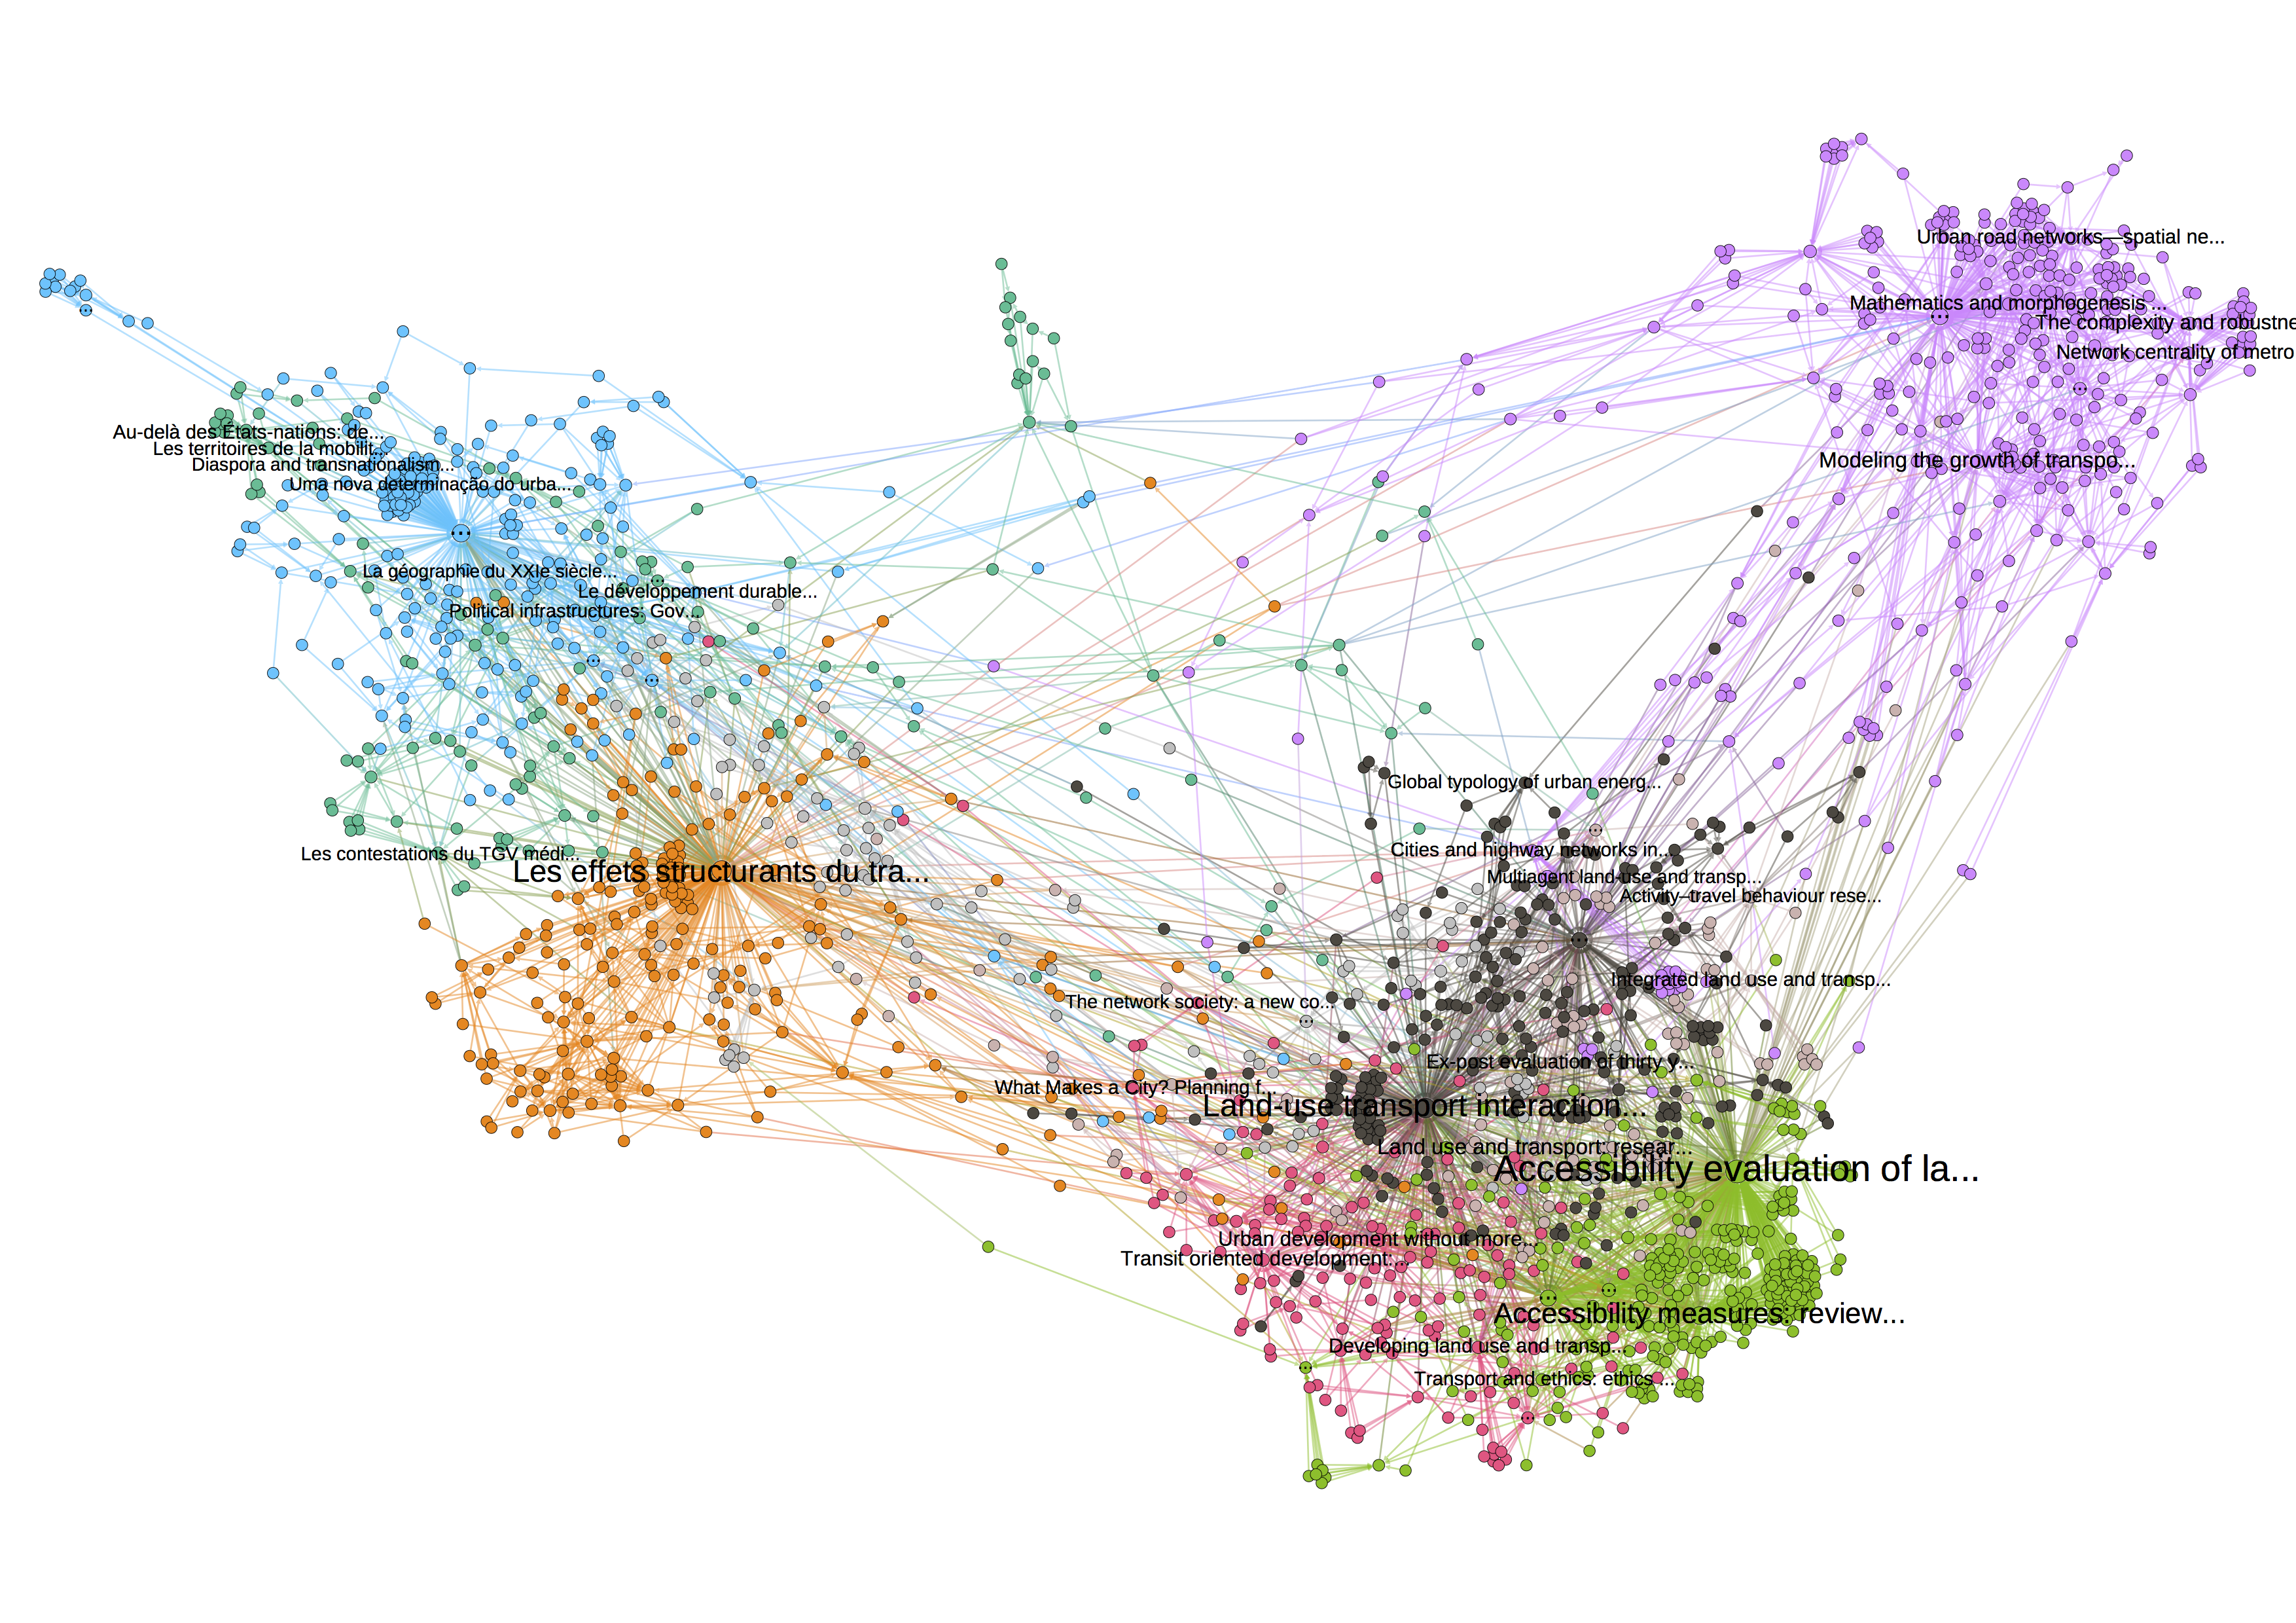
\includegraphics[width=\linewidth]{Figures/QuantEpistemo/rawcore}
\caption[Citation Network][Réseau de citations]{\textbf{Citation Network}\label{fig:quantepistemo:citnw}}{\textbf{Réseau de citations.} Nous visualisons les références ayant au moins deux liens, par un algorithme de force-atlas. Les couleurs donnent les communautés décrites dans le texte. En orange, bleu, turquoise: géographie urbaine, géographie des transports, sciences politiques ; en rose, noir, vert: planning, accessibilité, LUTI ; en violet : réseaux spatiaux (physique et économie).\label{fig:quantepistemo:citnw}}
\end{figure}
%%%%%%%%%%%%%%%%%





%%%%%%%%%%%%%%%%%%
\paragraph{Semantic Communities}{Communautés Sémantiques}


L'extraction des mots-clés est faite suivant une heuristique inspirée de~\cite{chavalarias2013phylomemetic}. La description complète de la méthode et de son implémentation est donnée en Appendice~\ref{app:sec:cybergeo}. Elle se base sur les relations au second ordre entre les entités sémantiques, qui sont des \emph{n-grams}, c'est à dire des mots-clés multiples pouvant avoir une longueur jusqu'à 3. Celles-ci sont estimées via la matrice de co-occurrence, dont les propriétés statistiques fournissent une mesure de déviation à des co-occurrences uniformes, qui est utilisée pour juger la pertinence des mots-clés. Sélectionnant un nombre fixe de mots-clés pertinents $K_W = 10000$, nous pouvons ensuite construire un réseau pondéré par les co-occurrences.


\bpar{
The topology of raw networks does not allow the extraction of clear communities, in particular because of the presence of hubs that correspond to frequent terms common to many fields (e.g. \texttt{model}, \texttt{space}). We assume these highest degree terms do not carry specific information on particular classes and can be thus filtered given a maximal degree threshold $k_{max}$. Similarly, edge with small weight are considered as noise and filtered according to a minimal edge weight threshold $\theta_w$. Keywords are preliminary filtered by a document frequency window $\left[ f_{min},f_{max} \right]$ which is slightly different from network filtering and complementary. A sensitivity analysis of resulting network topology to these parameters is presented in Fig.~\ref{fig:sensitivity}. We choose parameter values that maximize modularity under the constraint of a community number and size distribution of same magnitude as technological classes. This multi-objective optimization does not have a unique solution as objectives are somehow contradictory, and a compromise point must be chosen.
}{
La topologie du réseau brut ne permet pas l'extraction claire de communautés, en particulier à cause de hubs qui correspondent à des termes fréquents commun à de nombreux champs (e.g. \texttt{model}, \texttt{space})\comment[FL]{statut de ces mots ?}. Nous faisons l'hypothèse que ces termes à fort degré ne portent pas d'information particulière sur des classes données et peuvent ainsi être filtrés étant donné un seuil de degré maximal $k_{max}$ (on s'intéresse alors à ce qui fait la spécificité de chaque domaine). De la même manière, les liens avec un poids faibles sont considérés comme du bruit et filtrés selon un seuil de poids minimal $\theta_w$. La méthode générique permet de plus une filtration préliminaire des mot-clés, complémentaire à la filtration topologique, par fréquence d'apparition dans les documents $\left[ f_{min},f_{max} \right]$, à laquelle les résultats ne sont pas sensibles dans notre cas. L'analyse de sensibilité des caractéristiques du réseau filtré, notamment de sa taille, modularité et structure des communautés, est donnée en~\ref{app:sec:quantepistemo}. Nous choisissons des valeurs de paramètres permettant une optimisation multi-objectif entre modularité et taille du réseau, $\theta_w = 10,k_{max} = 500$, par le choix d'un point compromis sur un front de Pareto, qui donne un réseau sémantique de taille $(V=7063,E=48952)$. Celui-ci est visualisé en Appendice~\ref{app:sec:quantepistemo}.
}


\bpar{
We then retrieve communities in the semantic network (using standard Louvain algorithm, with the optimized filtering parameters). communities correspond to well-defined scientific fields (and/or domains, approaches). An expert validation allow us to give names to these, a more complicated naming procedure would eventually be possible (as in~\cite{yang2000improving} for the case of patents 
 where a chi-square test on distribution of documents in classes), but we prefer to stick here to a certain level of supervision. Table~\ref{tab:domains} summarizes the communities 
}{
Nous récupérons ensuite les communautés dans le réseau par un clustering de Louvain standard sur le réseau filtré optimal. On obtient 20 communautés pour une modularité de 0.58. Celles-ci sont examinées à la main pour être nommées, les techniques de désignation automatique~\cite{yang2000improving} n'étant pas assez élaborées et ne font pas la distinction implicite entre champs thématiques et méthodologiques par exemple (en fait entre les domaines de connaissance, voir~\ref{sec:knowledgeframework}) qui est une dimension supplémentaire que nous ne traitons pas ici, mais nécessaire pour avoir des désignations parlantes. Les communautés sont décrites en Table~\ref{tab:quantepistemo:semanticdomains}. On voit tout de suite la complémentarité avec l'approche par citation, puisque se dégagent ici à la fois des sujet d'étude (High Speed Rail, Maritime Networks), des domaines et méthodes (Networks, Remote Sensing, Mobility Data Mining), des domaines thématiques (Policy), des méthodes pures (Agent-based Modeling, Measuring). Ainsi, une référence peut mobiliser plusieurs de ces communautés. On a de plus une granularité plus fine de l'information. L'effet du langage est puissant puisque la géographie française se distingue en une catégorie séparée (des analyses poussées pourraient être envisagées pour mieux comprendre le phénomène et en tirer parti: sous-communautés, reconstruction d'un réseau spécifique, études par traduction ; mais celles-ci sont hors de propos dans cette étude exploratoire). On constante l'importance des réseaux, des problématiques de sciences politiques et socio-économiques. Nous mobiliserons la première catégorie dans la plupart des modèles développés, mais en gardant en tête l'importance des problématiques liées à la gouvernance, nous réaliserons un travail spécifique en~\ref{sec:lutetia}.
}




%%%%%%%%%%%%%%%%%%
\begin{table}
\caption[Semantic communities][Communautés sémantiques]{Disciplines/domains/fields reconstructed from community detection in the semantic network}{\textbf{Description des communautés sémantiques.} On donne leur taille, leur proportion en quantité de mots-clés cumulés sur l'ensemble du corpus, et des mots-clés représentatifs sélectionnés par degré maximal.\comment[FL]{pourquoi ces mots sont ils tronques ?}[(JR) cest explique dans le texte (surtout en annexe) il s'agit de stem]}
\label{tab:quantepistemo:semanticdomains}
\begin{tabular}{llll}
\hline\noalign{\smallskip}
Name & Size & Weight & Keywords  \\
\noalign{\smallskip}\hline\noalign{\smallskip}
Networks & 820 & 13.57\% & \texttt{social network, spatial network, resili} \\
Policy & 700 & 11.8\% & \texttt{actor, decision-mak, societi} \\
Socio-economic & 793 & 11.6\% & \texttt{neighborhood, incom, live} \\
High Speed Rail & 476 & 7.14\% & \texttt{high-spe, corridor, hsr} \\
French Geography & 210 & 6.08\% & \texttt{système, développement, territoire} \\
Education & 374 & 5.43\% & \texttt{school, student, collabor} \\
Climate Change & 411 & 5.42\% & \texttt{mitig, carbon, consumpt} \\
Remote Sensing & 405 & 4.65\% & \texttt{classif, detect, cover} \\
Sustainable Transport & 370 & 4.38\% & \texttt{sustain urban, travel demand, activity-bas} \\
Traffic & 368 & 4.23\% & \texttt{traffic congest, cbd, capit} \\
Maritime Networks & 402 & 4.2\% & \texttt{govern model, seaport, port author} \\
Environment & 289 & 3.79\% & \texttt{ecosystem servic, regul, settlement} \\
Accessibility & 260 & 3.23\% & \texttt{access measur, transport access, urban growth} \\
Agent-based Modeling & 192 & 3.18\% & \texttt{agent-bas, spread, heterogen} \\
Transportation planning & 192 & 3.18\% & \texttt{transport project, option, cba} \\
Mobility Data Mining & 168 & 2.49\% & \texttt{human mobil, movement, mobil phone} \\
Health Geography & 196 & 2.49\% & \texttt{healthcar, inequ, exclus} \\
Freight and Logistics & 239 & 2.06\% & \texttt{freight transport, citi logist, modal} \\
Spanish Geography & 106 & 1.26\% & \texttt{movilidad urbana, criteria, para} \\
Measuring & 166 & 1.0\% & \texttt{score, sampl, metric} \\
\noalign{\smallskip}\hline
\end{tabular}
\end{table}
%%%%%%%%%%%%%%%%%%



%%%%%%%%%%%%%%%%%%
\paragraph{Measures of Interdisciplinarity}{Mesures d'interdisciplinarité}


\bpar{
Distribution of keywords within communities provides an article-level interdisciplinarity.
Combination of citation and semantic layers in the hyper-network provide second order interdisciplinarity measures, that we don't use here because of the modest size of the citation network. More precisely, a reference can be viewed as a probability vector on semantic classes.
}{
La distribution des mots clés dans les communautés permettent de définir une mesure d'interdisciplinarité au niveau de l'article. La combinaison des couches de citation et sémantique dans l'hyperréseau fournit des mesures d'interdisciplinarité au second ordre (motifs sémantiques des cités ou des citants), que nous n'utiliserons pas ici à cause de la taille modeste du réseau de citation (voir \ref{app:sec:cybergeo} et \ref{app:sec:patents}). Plus précisément, une référence $i$ peut être vue comme un vecteur de probabilités sur les classes sémantiques $j$, qu'on notera sous forme matricielle $\mathbf{P}=(p_{ij})$. Celles-ci sont estimées simplement par les proportions de mots-clés classifiés dans chaque classe pour la référence. Une mesure classique d'interdisciplinarité~\cite{bergeaud2017classifying} est alors $I_i = 1 - \sum_j p_{ij}^2$. Soit $\mathbf{A}$ la matrice d'adjacence du réseau de citation, et soit $\mathbf{I}_k$ les matrices de selection des lignes correspondants à la classe $k$ de la classification de citation: $Id\cdot \mathbbm{1}_{c(i)=k}$, telle que $I_k \cdot A \cdot I_{k'}$ donne exactement les citations de $k$ vers $k'$. La proximité de citation entre les communautés de citation est alors définie par $c_{kk'} = \sum \mathbf{I}_k \cdot \mathbf{A} \cdot \mathbf{I}_{k'} /  \sum \mathbf{I}_k \cdot \mathbf{A}$. On définit la proximité sémantique en définissant une matrice de distance entre références par $\mathbf{D} = d_{ii'}=\sqrt{\frac{1}{2}\sum (p_{ij}-p{i'j})^2}$ puis la proximité sémantique par $s_{kk'} = \mathbf{I}_k \cdot \mathbf{D} \cdot \mathbf{I}_{k'} / \sum \mathbf{I}_k \sum \mathbf{I}_{k'}$. Nous montrons en Fig.~\ref{fig:quantepistemo:interdisc} les valeurs de ces différentes mesures, ainsi que la composition sémantique des communautés de citation, pour les classes sémantiques majoritaires. La distribution de $I_i$ montre que les papiers gravitant dans le domaine du LUTI sont les plus interdisciplinaires dans les termes utilisés, ce qui pourrait être lié à leur caractère appliqué. Les autres disciplines sont dans des motifs similaires, à part la géographie et la planification des infrastructures qui présentent des distributions quasi-uniformes, témoignant de l'existence de références très spécialisées dans ces classes. Ce n'est pas nécessairement étonnant vu les sous-champs pointus exhibés (sciences politiques par exemples, et de même les études prospectives type coût-bénéfices sont très étriquées). Ce premier croisement des couches nous confirme les spécificités de chaque champ. Concernant les compositions sémantiques, la plupart agissent comme validation externe vu les classes majoritaires. Le champ le moins concerné par les problème socio-économiques est la planification des infrastructure, ce qui donnera du grain à moudre aux détracteurs de la technocratie. Les questions de changement climatique et durabilité sont relativement bien répartie. Enfin, les ouvrages géographiques concernent en majorité des problèmes de gouvernance. Les matrices de proximité confirment la conclusion de la sous-section précédente en terme de citation, les partages étant très faibles, les plus hautes valeurs étant jusqu'à un quart de la planification vers la géographie et des LUTI vers le TOD (mais pas l'inverse, les relations peuvent être à sens unique). Hors, les proximités sémantiques montrent par exemple que LUTI, TOD, Accessibility et Networks sont proches dans leur termes, ce qui est logique pour les trois premiers, et confirme pour le dernier que les physiciens se basent majoritairement sur les méthodes des ces champs liés au planing pour légitimer leur travaux. La géographie est totalement isolée, sa plus proche voisine étant la planification des infrastructures. Cette étude est très utile pour notre propos, puisqu'elle montre des domaines cloisonnés partageant des termes at donc a priori des problématiques et sujet commun. On ne se parle pas alors qu'on parle des languages pas si lointains, d'où la pertinence accrue de les faire parler d'une commune voie dans nos travaux : nos modèles devront mobiliser des éléments, ontologies et échelles de ces différents champs.
}



%%%%%%%%%%%%%%%%%%
\begin{figure}
\includegraphics[width=0.49\linewidth]{Figures/QuantEpistemo/interdisciplinarities}
\includegraphics[width=0.49\linewidth]{Figures/QuantEpistemo/compo_proportion}\\
\includegraphics[width=0.49\linewidth]{Figures/QuantEpistemo/citation_proximities}
\includegraphics[width=0.49\linewidth]{Figures/QuantEpistemo/semantic_proximities}
\caption[][Motifs d'interdisciplinarité]{\label{fig:quantepistemo:interdisc}}{\textbf{Motifs d'interdisciplinarité.} \textit{(Haut Gauche)} Distribution des $I_i$ par classes de citations ; \textit{(Haut Droite)} Composition sémantiques des classes de citation ; \textit{(Bas Gauche)} Matrice de proximité de citation $c_{kk'}$ entre classes de citations ; \textit{(Bas Droite)} Matrice de proximité sémantique $s_{kk'}$ entre classes de citations.\label{fig:quantepistemo:interdisc}\comment[FL]{tu compares les disciplines entre elles mais pas la facon dont elles attaquent les questions au coeur de ta these. c'est dommage.}[(JR)c'est l'objet de la section suivante]}
\end{figure}
%%%%%%%%%%%%%%%%%%



% bootstrap
%min(corrs);max(corrs);mean(abs(corrs))
% -0.170952  0.5496791  0.08384802
% apply(bcorrs,2,mean)
%       minrho        maxrho    meanabsrho     minrhosup     maxrhosup meanabsrhosup 
%  -0.08792137    0.11690677    0.03137750   -0.17686637    0.68579406    0.11079253 
% apply(bcorrs,2,sd)
%       minrho        maxrho    meanabsrho     minrhosup     maxrhosup meanabsrhosup 
%  0.012683338   0.021324056   0.002250636   0.038402781   0.134996447   0.051553244 

% modularities
% sem : 0.1053156
% cit : 0.8140818
% bootstrap N=100
% sem : 0.073097051446193 +- 0.00307154703966512
% cit : 0.204223565075042 +- 0.0141450119581389


\bpar{
}{
Nous concluons cette analyse par une approche plus robuste pour quantifier les proximités entre couches de l'hyperréseau. Il est aisé de construire une matrice de corrélation entre deux classifications, par les corrélations de leur colonnes. Nous définissons les probabilités $\mathbf{P}_C$ toutes égales à 1 pour la classification de citation. La matrice de correlation de celle-ci avec $\mathbf{P}$ s'étend de -0.17 à 0.54 et a une moyenne de valeur absolue de 0.08, ce qui est significatif par rapport à des classifications aléatoire puisque un bootstrap à $b=100$ répétitions avec les matrices mélangées donne un minimum à $-0.08 \pm 0.012$, un maximum à $0.11 \pm 0.02$ et une moyenne absolue à $0.03 \pm 0.002$. Cela montre que les classifications sont complémentaires et que cette complémentarité est significative statistiquement par rapport à des classifications aléatoires. L'adéquation de la classification sémantique par rapport au réseau de citation peut également être quantifiée par la modularité multi-classes~\cite{nicosia2009extending} (voir~\ref{sec:app:patents} pour une définition mathématique), qui traduit la probabilité qu'un lien soit dû à la classification étudiée, en prenant en compte l'appartenance simultanée à de multiples classes. Ainsi, la modularité multi-classes des probabilités sémantiques pour le réseau de citation est de 0.10, ce qui d'une part est significativement signe d'adéquation, un bootstrap toujours à $b=100$ donnant une valeur de $0.073 \pm 0.003$, qui reste limitée vu la valeur maximale fixée par les probabilités de citations dans leur propre réseau qui donnent une valeur de 0.81, ce qui confirme d'autre part la complémentarité des classifications.
}








%--------------------------------------------------------------



%%%%%%%%%%%%%%%%%%%%%%%%
\subsection{Discussion}{Discussion}




\subsubsection{Towards modeling purpose and context automatic extraction}{Vers une modélisation des thèmes et une extraction automatique du contexte}


\bpar{
A possible direction to strengthen our quantitative epistemological analysis would be to work on full textes related to the modeling of interaction between networks and territories, with the aim to automatically extract thematics within articles. The idea would be to perform some kind of automatized modelography, with possible features to be extracted that would be ontologies, model architecture or structures, scales, or even typical parameter values. It is not clear to what degree structure of models can be extracted from their description in papers and it surely depends on the discipline considered. For example in a framed field such as transportation planning, using a pre-defined ontology (in the sense of dictionary) and a fuzzy grammar could be efficient to extract information as the discipline is relatively formatted. In theoretical and quantitative geography, beyond the barrier of language, information organisation is surely less subject to unsupervised data-mining because of the more literary nature of the discipline : synonyms and figures of speech are generally the norm in good level human sciences writing, fuzzing a possible generic structure of knowledge description. 
}{
Une direction possible pour renforcer cette analyse en épistémologie quantitative serait de travailler sur les textes complets des références contenant des efforts de modélisations des interactions entre réseaux et territoires, avec le but d'extraire automatiquement les thématiques des articles. Des méthodes plus adaptées pour les long texte que celle utilisée ici incluent par exemple l'Allocation Latente de Dirichlet~\cite{blei2003latent}. L'idée serait de procéder à une sorte de modélographie automatique, pour extraire des caractéristiques telle les ontologies, l'architecture ou la structure des modèles, les échelles ou même des valeurs typiques des paramètres. Il n'est pas clair dans quelle mesure la structure des modèles peut être extraite de leur description dans un article, et cela dépend sûrement de la discipline considérée. Par exemple dans champ relativement cadré comme la planification des transports, l'utilisation d'une ontologie pré-définie (dans le sens d'un dictionnaire) et d'une grammaire floue pourrait être efficace vu les conventions assez strictes dans la discipline. En géographie théorique et quantitative, au delà de la barrière du language\comment[FL]{?}, l'organisation de l'information est sûrement plus délicate à appréhender par de l'apprentissage non-supervisé à cause de la nature plus littéraire de la discipline : les synonymes et les figures de style sont généralement la norme pour l'écriture d'un bon niveau en sciences humaines, rendant plus floue une possible structure générique de la description des connaissances.
}


%Depending on extended results of the two previous sections and on thematic requirements (huge need of knowledge on precise models structure, that may appear when trying to construct more specialized operational models), this project may be conducted with more or less investment.




\subsubsection{Reflexivity}{Réflexivité}


\bpar{
The methodology developed here is particularly interesting since it is reflexive, i.e. it can be used on our work itself. Therefore, an other application will be the reflexivity of our thesis : we attend to proceed to similar analysis on our proper bibliography (and possibly its evolution, available via \texttt{git} history), to understand our patterns of knowledge, possible gaps or unveil unexpected developments. The detailed development is done in Appendix~\ref{app:reflexivity}.
}{
La méthodologie que nous avons développé ici est particulièrement intéressante puisqu'elle offre des potentialités de réflexivité, c'est à dire qu'elle peut être utilisée pour étudier notre approche elle-même. Une de ses applications, hors de celle à la revue scientifique Cybergeo dans la perspective de Science Ouverte (voir Appendice~\ref{app:sec:cybergeo}), sera à notre propre corpus de références, dans le but de révéler des possibles  directions de recherche ou problématiques exotiques. Il est éventuellement possible de le faire de manière dynamique, grâce à l'historique de \texttt{git} qui permet de récupérer n'importe quelle version de la bibliographie à une date donnée sur les trois ans écoulés. Il s'agira aussi de comprendre nos motifs de production de connaissance afin de contribuer à~\ref{sec:knowledgeframework}. Le développement détaillé est fait en Appendice~\ref{app:reflexivity}.
}





\stars




%%%%%%%%%%%%%%%%%



%%%%%%%%%%%%%%%%%
% Modelography


% -> TODO Systematic Review

\comment[JR]{la modélographie doit logiquement arriver après les études d'épistemo quanti, qui ont permis de donner un aperçu de l'horizon scientifique}



\section{Systematic Review and Modelography}{Revue Systématique et Modélographie}


An ongoing work is the production of a synthesis of this overview, from a modular modeling point of view, combined with a purpose and scale classification. Already mentioned, modular modeling consists in the integration of heterogeneous processes and implementation of processes in order to extract the set of mechanisms giving the best fit to empirical data~\cite{cottineau2015incremental}. We can thus classify models described here according to their building bricks in terms of processes implemented and thus identify possible coupling potentialities. This work is a preliminary step for the analysis in quantitative epistemology developed in chapter~\ref{ch:quantepistemo}.



%%%%%%%%%%%%%%%%%%%%
\subsection[Systematic Review][Revue Systématique]{Systematic Review and Meta-analysis}{Revue systématique et Meta-analyse}


Tandis que les études menées précédemment proposaient de construire un horizon global de l'organisation des disciplines s'intéressant à notre question, nous proposons à présent une étude plus ciblée des caractéristiques de modèles existants. Nous proposons pour cela dans un premier temps une revue systématique, c'est à dire la construction d'un corpus répondant à certaines contraintes, suivie d'une meta-analyse, c'est à dire une tentative d'explication de certaines caractéristiques des modèles par des modèles statistiques.

\comment[JR]{également tenter une classif endogène des modèles : selon les caractéristiques récupérées.}











%%%%%%%%%%%%%%%%%%%%
\subsection{Modelography}{Modélographie}


Nous passons à présent à une analyse qualitative inspirée par les résultats précédents, notamment pour la classification. Elle a pour but d'extraire et de décomposer précisément les ontologies, échelles et processus.














%%%%%%%%%%%%%%%%%%%%
\subsection{Discussion}{Discussion}







%%%%%%%%%%%%%%%%%


%
% 2.1 - State of the Art




%----------------------------------------------------------------------------------------

\newpage

\section{Modeling Interactions}{Modéliser les Interactions}
\label{sec:modelingsa}


%----------------------------------------------------------------------------------------




\subsection{Modeling in Quantitative Geography}{Modélisation en Géographie Quantitative}


\subsubsection{History}{Histoire}

\bpar{
Modeling in Theoretical and Quantitative Geography (TQG), and more generally in Social Science, has a long history on which we can not go further than a general context. \noun{Cuyala} does in~\cite{cuyala2014analyse} an analysis of the spatio-temporal development of French speaking TQG movement and underlines the emergence of the discipline as the combination between quantitative analysis (e.g. spatial analysis or modeling and simulation practices) and theoretical constructions, an integration of both allowing the construction of theories from empirical stylized facts that yield theoretical hypothesis to be tested on empirical data. These approach were born under the influence of the \emph{new geography} in Anglo-saxon countries and Sweden.
}{
La modélisation joue en Géographie Théorique et Quantitative (TQG) un rôle fondamental. \cite{cuyala2014analyse} procède à une analyse spatio-temporelle du mouvement de la Géographie Théorique et Quantitative en langue française et souligne l'émergence de la discipline comme une combinaison d'analyses quantitatives (e.g. analyse spatiale et pratiques de modélisation et de simulation) et de construction théoriques. Cette dynamique est datée à la fin des années 70, et est intimement liée à l'utilisation et l'appropriation des outils mathématiques~\cite{pumain2002role}. L'intégration de ces deux composantes permet la construction de théories à partir de faits stylisés empiriques, qui produisent à leur tour des hypothèses théoriques pouvant être testées sur les données empiriques. Cette approche est née sous l'influence de la \emph{New Geography} dans les pays Anglo-saxons et en Suède. Concernant la modélisation urbaine en elle-même, d'autre champs que la géographie ont proposé des modèles de simulation à peu près à la même période. Par exemple, le modèle de \noun{Lowry}, développé par~\cite{lowry1964model} dans un but appliqué immédiat à la région métropolitaine de Pittsburg, suppose un système d'équations pour la localisation des actifs et des emplois dans différente zones. Des modèles relativement similaires sont toujours utilisés aujourd'hui.
}


%\comment[FL]{manque peut etre quelques phrases avec des modeles ``landmark'' anciens (Lowry 1964 par exemple) mais encore utilises, de plus ne pas perdre le fil du champ applicatif auquel tu te destines}

% Lowry : https://www.rand.org/content/dam/rand/pubs/research_memoranda/2006/RM4035.pdf
% Alonso : http://onlinelibrary.wiley.com/doi/10.1111/j.1435-5597.1967.tb01370.x/epdf
% http://www.sciencedirect.com/science/article/pii/S009411909792074X prefatt-diff ?


\subsubsection{Simulation of models and intensive computation}{Simulation de modèle et calcul intensif}


\bpar{
A broad history of the genesis of models of simulation in geography is done by \noun{Rey} in~\cite{rey2015plateforme} with a particular emphasis on the notion of validation of models. The use of computation for simulation of models is anterior to the introduction of paradigms of complexity, coming back to \noun{H{\"a}gerstrand} and \noun{Forrester}, pioneers of spatial economic models inspired by Cybernetics. With the increase of computational possibilities epistemological transformations have also occurred, with the apparition of explicative models as experimental tools. \noun{Rey} compares the dynamism of seventies when computation centers were opened to geographers to the democratization of High Performance Computing (transparent grid computing, see~\cite{schmitt2014half} for an exemple of the possibilities offered in terms of model validation and calibration, decreasing the computational time from 30 years to one week), that is also accompanied by an evolution of modeling practices~\cite{banos2013pour} and techniques~\cite{10.1371/journal.pone.0138212}.
}{
Une histoire étendue de la genèse des modèles de simulation en géographie est faite par \noun{Rey} dans~\cite{rey2015plateforme} avec une attention particulière pour la notion de validation de modèles (nous reviendrons sur la place de ces aspects dans notre travail en~\ref{ch:positioning}). L'utilisation de ressources de calcul pour la simulation de modèles est antérieure à l'introduction des paradigmes de la complexité actuels, remontant par exemple à \noun{Forrester}, informaticien qui a été pionnier des modèles d'économie spatiale inspirés par la cybernétique\footnote{Celle-ci, ainsi que le courant systémique, sont comme nous l'avons déjà développé précurseurs des paradigmes actuels de la complexité.}. Avec l'augmentation des potentialités de calcul, des transformations épistémologiques ont également suivi, avec l'apparition de models explicatifs comme outils expérimentaux. \noun{Rey} compare le dynamisme des années soixante-dix quand les centres de calcul furent ouverts aux géographes à la démocratisation actuelle du Calcul Haute Performance. Aujourd'hui, cette facilité d'accès consiste entre autres à du calcul sur grille dont l'utilisation est rendue transparente, c'est à dire sans besoin de compétences techniques pointues liées au mécanismes de la distribution des calculs.. Ainsi~\cite{schmitt2014half} donnent un exemple des possibilités offertes en termes de calibration et de validation de modèle, réduisant le temps de calcul nécessaire de 30 ans à une semaine - ces techniques jouent un rôle clé pour les résultats que nous obtiendrons par la suite. Cette évolution est également accompagnée par une évolution des pratiques~\cite{banos2013pour} et techniques~\cite{10.1371/journal.pone.0138212} de modélisation.
}


\bpar{
Modeling (in particular computational models of simulation) is seen by many as a fundamental building brick of knowledge : \cite{livet2010} recalls the combination of empirical, conceptual (theoretical) and modeling domains with constructive feedbacks between each. A model can be an exploration tool to test assumptions, an empirical tool to validate a theory against datasets, an explicative tool to reveal causalities (and thus internal processes of a system), a constructive tool to iteratively build a theory with an iterative construction of an associated model. These are example among others : \noun{Varenne} proposes in~\cite{varenne2010simulations} a refined classifications of diverse functions of a model. We will consider modeling as a fundamental instrument of knowledge on processes within complex adaptive systems, as already evoked, and restraining again our question, will focus on \emph{models involving interactions between transportation networks and territories}.
}{
La modélisation, et en particulier les modèles de simulation, est vue par beaucoup comme une brique fondamentale de la connaissance : \cite{livet2010} rappelle la combinaison des domaines empirique, conceptuel (théorique) et de la modélisation, avec des retroactions constructives entre chaque. Un modèle peut être un outil d'exploration pour tester des hypothèses, un outil empirique pour valider une théorie sur des jeux de données, un outil explicatif pour révéler des causalités et ainsi des processus internes au système, un outil constructif pour construire itérativement une théorie conjointement avec celle des modèles associés. Ce sont des exemples de fonctions parmi d'autres : \cite{varenne2010simulations} propose une classification des diverses fonctions d'un modèle. Nous considérons la modélisation comme un instrument fondamental de connaissance des processus au sein d'un système, plus particulièrement dans notre cas au sein d'un système complexe adaptatif. Nous rappelons ainsi que notre question de recherche s'intéressera aux \emph{modèles dont l'ontologie contient une part non négligeable d'interactions réseaux et territoires}.
}




%%%%%%%%%%%%%%%%%%%%%%%%%%%
\subsection{Modeling Territories and Networks}{Modéliser les territoires et réseaux}


\bpar{
Concerning our precise question of interactions between transportation networks and territories, we propose an overview of existing approaches. Following~\cite{bretagnolle2002time}, the ``\textit{thoughts of specialists in planning aimed to give definitions of city systems, since 1830, are closely linked to the historical transformations of communication networks}''. It is not far from an reversed self-realizing prophecy, in the sense that it is already realized before happening. It implies that ontologies and corresponding models addressed by geographers and planners are closely linked to their current historical preoccupations, thus necessarily limited in scope and purpose. In a perspectivist vision of science~\cite{giere2010scientific} such boundaries are the essence of the scientific entreprise, and as we will argue in chapter~\ref{ch:theory} their combination and coupling in the case of models is a source of knowledge.
}{
Développons à présent un aperçu des différentes approches modélisant des interactions entre réseaux de transport et territoires. Remarquons de manière préliminaire une forte contingence des constructions scientifiques sous-jacentes à celles-ci. En effet, selon~\cite{bretagnolle2002time}, ``\textit{les idées des spécialistes de la planification cherchant à donner des définitions des systèmes de ville, depuis 1830, sont étroitement liées aux transformations des réseaux de communication}''. Le contexte historique (et donc socio-économique et technologique) conditionne fortement les théories formulées. %C'est en quelque sorte la prophétie auto-réalisatrice inversée, au sens où elle est déjà réalisée avant d'être formulée\comment[FL]{sens ?}. % -> notion de coevol des connaissance avec les objets - on revient sur la reflexivité - trop glissant pour développer.
 Cela implique que les ontologies et les modèles correspondants proposés par les géographes et les planificateurs sont fortement liés aux préoccupations historiques courantes, ce qui limite nécessairement leur portée théorique et/ou opérationnelle. Au delà de la question de la définition du système qui joue également un rôle central, on comprend bien l'impact que peut avoir cette influence sur la portée des modèles développés. Dans une vision perspectiviste de la science~\cite{giere2010scientific} de telles limites sont l'essence de l'entreprise scientifique, et comme nous démontrerons dans le chapitre~\ref{ch:theory} leur combinaison et couplage dans le cas de modèles est généralement une source de connaissance.
}

% \comment[FL]{pas par essence mais cela peut l'etre effectivement}[(JR) pas d'accord : opérer un couplage de modele implique un couplage des ontologies et necessairement un accroissement des connaissances (si celui-ci est utile c'est un autre problème)]


L'entrée que nous proposons ici pour dresser un aperçu des modèles est complémentaire de celle prise au Chapitre~\ref{ch:thematic}, en regardant par objet principal (c'est à dire les relations Réseau $\rightarrow$ Territoire, Territoire $\rightarrow$ Réseau et Territoire $\leftrightarrow$ Réseau). Nous avons vu que la correspondance à des échelles temporelles et spatiales n'est pas systématique (voir la typologie provisoire à double entrée des processus). Par contre, celle à des domaines particuliers et à des acteurs l'est plus. Cette revue de littérature est donc orientée dans cette seconde direction.

%\comment[FL]{tu arrives trop tot la dessus - les processus cles ne sont pas ammenes suffisamment clairement : travaille par echelle de temps, d'espace, d'acteurs}[ok developper en echo au 1 - vision par les acteurs / vision par les echelles.]


%\subsubsection{Land-Use Transportation Interaction Models}{Modèles LUTI}
\subsubsection{Territories}{Territoires}


Le courant principal s'intéressant à la modélisation de l'influence du réseau de transport sur les territoires se trouve dans le champ de la planification, à des échelles spatiales et temporelles moyennes (les échelles de l'accessibilité métropolitaine que nous avons développés ci-dessus). Des modèles en géographie à d'autres échelles, comme les modèles Simpop déjà évoqués~\cite{pumain2012multi}, ne supposent pas une ontologie particulière pour le réseau de transport, et sont relativement éloignés de l'idée d'interaction. Nous reviendrons plus loin sur des extensions pertinentes pour notre question. Revoyons pour commencer le contexte des études de planification.


\paragraph{LUTI models}{Modèles LUTI}

\bpar{
A subsequent bunch of literature in modeling interaction between networks and territories can be found in the field of planning, with the so-called \emph{Land-use Transportation Interaction Models}. These works are difficult to be precisely bounded as they may be influenced by various disciplines. For example, from the point of view of Urban Economics, propositions for integrated models have existed for a relatively long term~\cite{putman1975urban}.
}{
Ces approches sont désignées de manière générale comme \emph{modèles d'interaction entre usage du sol et transport} (\emph{LUTI}, pour \textit{Land-Use Transport Interaction}). Il est entendu par usage du sol la répartition des activités territoriales, généralement réparties en typologies plus ou moins précises (par exemple logements, industrie, tertiaire, espace naturel). Ces travaux peuvent être difficiles à cerner car liés à différentes disciplines scientifiques. Leur principe général est de modéliser et simuler l'évolution de la distribution spatiale des activités, en prenant le réseau de transport comme contexte et déterminant significatif des localisations. Par exemple, du point de vue de l'Economie Urbaine, les propositions de tels modèles existent depuis un certain temps : \cite{putman1975urban} rappelle le cadre d'économie urbaine où les principales composantes sont les emplois, la démographie et le transport, et passe en revue des modèles économiques de localisation qui s'apparentent au modèle de \noun{Lowry}.
}


\bpar{
Generally these type of models operate at relatively small temporal and spatial scales. \cite{wegener2004land} reviewed state of the art in empirical and modeling studies on interactions between land-use and transportation. It is positioned in economic, planning and sociological theoretical contexts, and is relatively far from our geographical approach aiming to also understand long-time processes. Seventeen models are compared and classified, none of which implements actually network endogenous evolution on the relatively small time scales of simulation. A complementary review done in \cite{chang2006models} broadens the scope with inclusion of more general classes of models, such as spatial interaction models (including traffic assignment and four steps models), operational research planning models (optimal localisations), micro-based random utility models, and urban market models.
}{
\cite{wegener2004land} donne plus récemment un état de l'art des études empiriques et de modélisation sur ce type d'approche des interactions entre usage du sol et transport. Le positionnement théorique est plutôt proche des disciplines de la socio-économie des transports et de la planification (voir les paysages disciplinaires dressés en~\ref{sec:quantepistemo}). \cite{wegener2004land} compare et classifie dix-sept modèles, parmi lesquels aucun n'inclut une évolution endogène du réseau de transport sur les échelles de temps relativement courtes (de l'ordre de la décade) des simulations. On retrouve bien la correspondance avec les échelles typiquement mesoscopiques établies précédemment. Une revue complémentaire est faite par~\cite{chang2006models}, élargissant le contexte avec l'inclusion de classes plus générales de modèles, comme des modèles d'interactions spatiales (parmi lesquels l'attribution du traffic et les modèles à quatre temps), les modèles de planification basés sur la recherche opérationnelle (optimisation des localisations des différentes activités, généralement résidences et emplois), les modèles microscopiques d'utilité aléatoire, et les modèles de marché foncier.
}




\paragraph{Operational models}{Des modèles opérationnels très variés}


\bpar{The variety of possible models has lead to operational comparisons~\cite{paulley1991overview,wegener1991one}.}
{
La variété des modèles existants a conduit à des comparaisons opérationnelles : \cite{paulley1991overview} rendent compte d'un projet comparant différents modèles appliqués à différentes villes. Leurs résultats permettent d'un part de classifier des interventions en fonction de leur impact sur le niveau d'interaction entre transport et usage du sol, et d'autre part de montrer que l'effet des interventions dépend fortement de la taille de la ville et de ses caractéristiques socio-économiques.
}


\bpar{
More recently, the respective advantages of static and dynamic modeling was investigated in~\cite{kryvobokov2013comparison}.
}{
Les ontologies des processus, et notamment sur la question de l'équilibre, sont aussi variées. Les avantages respectifs d'une approche statique (calcul d'un équilibre statique de la localisation des ménages pour une certaine spécification de leur fonctions d'utilité) et d'une approche dynamique (simulation hors équilibre des dynamiques résidentielles) a été étudié par~\cite{kryvobokov2013comparison}, dans un cadre métropolitain sur des échelles de temps de l'ordre de la décade. Les auteurs montrent que les résultats sont globalement comparables et que chaque modèle a son utilité selon la question posée.% Dans tous les cas, ce type de modèle opère généralement à des échelles temporelles et spatiales relativement faibles.
}



\bpar{
These techniques operate also at small scales and consider at most land-use evolution. \cite{iacono2008models} covers a similar scope with a further emphasis on cellular automata models of land-use change and agent-based models. These type of models are still largely developed and used today, as for example \cite{delons:hal-00319087} which is used for Parisian metropolitan region. The short-term range of application and their operational character makes them useful for planning, what is far from our preoccupation to obtain explicative models for geographical processes.
}{
Différents aspects du même système peuvent être traduits par divers modèles, comme le montre par exemple~\cite{wegener1991one}, et le trafic, les dynamiques résidentielles et d'emploi, l'évolution de l'usage du sol en découlant, influencée aussi par un réseau de transport statique, sont généralement pris en compte. \cite{iacono2008models} couvre un horizon similaire avec un développement supplémentaire sur les modèles à automates cellulaires d'évolution d'usage du sol et les modèles à base d'agents. Les modèles LUTI sont toujours largement étudiés et appliqués, comme par exemple \cite{delons:hal-00319087} qui est utilisé pour la région métropolitaine parisienne. La portée temporelle d'application de ces modèles, de l'ordre de la décade, et leur nature opérationnelle les rend utiles pour la planification, ce qui est assez loin de notre souci d'obtenir des modèles explicatifs de processus géographiques. En effet, il est souvent plus pertinent pour un modèle utilisé en planification d'être lisible comme outil d'anticipation, voire de communication, que d'être fidèle aux processus territoriaux au prix d'une abstraction.
}

%\comment[FL]{ce point est tres important et merite (un dvlpmt ?)}



\paragraph{Perspectives for LUTI models}{Perspectives pour les LUTI}

\bpar{}{
\cite{timmermans2003saga} émet des doutes quant à la possibilité de modèles d'interaction réellement intégrés, c'est à dire produisant des motifs de transports endogènes et se détachant d'artefacts comme l'accessibilité dont l'influence du caractère artificiel reste à établir, notamment à cause du manque de données et une difficulté à modéliser les processus de gouvernance et de planification. Il est intéressant de noter que les priorités actuelles de développement des modèles LUTI semblent centrées sur une meilleure intégration des nouvelles technologies et une meilleur intégration avec la planification et les processus de prise de décision, par exemple via des interfaces de visualisation comme le propose~\cite{JTLU611}. Ils ne cherchent pas à s'étendre à des problématiques de dynamiques territoriales incluant le réseau sur de plus longues échelles par exemple, ce qui confirme la portée et la logique d'utilisation et de développement de ce type de modèles.
}

\bpar{}{
Une généralisation de ce type d'approche à une plus grande échelle, comme celle proposée par \cite{russo2012unifying}, consiste au couplage du LUTI à l'échelle mesoscopique à des modèles macroéconomiques à l'échelle macroscopique. Ceux-ci ne considèrent pas l'évolution du réseau de transport de manière explicite mais s'intéressent seulement aux motifs abstraits d'offre et demande. L'économie urbaine a développé des approches spécifiques similaires dans leur démarche : \cite{masso2000} décrit par exemple un modèle intégré couplant développement urbain, relocalisation et équilibre des flux de transports.
}


\bpar{}{
Ainsi, nous pouvons synthétiser ce type d'approche, qu'on pourra désigner par abus de langage \emph{approche LUTI}, par les caractéristiques fondamentales suivantes : (i) Modèles visant à comprendre une évolution du territoire, dans le contexte d'un réseau de transport donné ; (ii) Modèles dans une logique de planification et d'applicabilité, étant souvent impliqués eux-même dans les prises de décision ; et (iii) Modèles à des échelles moyennes, dans l'espace (métropole) et dans le temps (décade).
}




\subsubsection{Network Growth}{Croissance du Réseau}

Passons à présent au paradigme ``opposé'', centré sur l'évolution du réseau. Il peut sembler incongru de considérer un réseau variable en négligeant les variations du territoire, au regard de l'aperçu de certains des mécanismes potentiels d'évolution revus précédemment (rupture de potentiel, auto-renforcements, planification du réseau) qui se produisent à des échelles de temps majoritairement plus longues que les évolutions territoriales. On verra ici qu'il n'y a pas de paradoxe, vu que (i) soit la modélisation s'intéresse à l'évolution des \emph{propriétés du réseau}, à une courte échelle (micro) pour des processus de congestion, de capacité, de tarification, principalement d'un point de vue économique ; (ii) soit les composantes territoriales jouant en effet sur le réseau sont stables au échelles longues considérés (approches des physiciens).


\bpar{
Network growth can be used to design modeling entreprises that aim to endogenously explain growth of transportation networks, generally from a bottom-up point of view, i.e. by exhibiting local rules that would allow to reproduce network growth over long time scales (generally the road network).
}{
La croissance de réseaux est l'objet de démarches de modélisation qui cherchent à expliquer la croissance des réseaux de transport. Ils prennent généralement un point de vue \emph{bottom-up} et endogène, c'est-à-dire cherchant à mettre en évidence des règles locales qui permettraient de reproduire la croissance du réseau sur de longues échelles de temps (souvent le réseau routier). Comme nous allons le voir, il peut s'agir de la croissance topologique (création de nouveaux liens) ou la croissance des capacités des liens en relation avec leur utilisation, selon les échelles et les ontologies considérées. Nous distinguons pour simplifier des grands courants disciplinaires s'étant intéressé à la modélisation de la croissance des réseaux de transport : ceux-ci sont liés respectivement à l'économie des transports, la physique, la géographie des transport et la biologie.
}


\bpar{
\cite{xie2009modeling} develops a broad review on network growth modeling extending to other fields: transportation geography early developed empirical-based models but which did concentrate on topology reproduction rather than on mechanisms according to~\cite{xie2009modeling}; statistical models on case studies provide mitigated conclusions on causal relations between offer and demand; economists have studied infrastructure provision from both microscopic and macroscopic point of views, generally non-spatial; network science has provided toy-models of network growth based on structural and topological rules rather on rules inspired from real processes.
}{
On rejoint ainsi partiellement la classification de~\cite{xie2009modeling}, qui propose une revue étendue de la modélisation de croissance des réseaux, dans une perspective d'économie des transports mais en élargissant à d'autres champs. Selon~\cite{xie2009modeling}, la géographie des transports a développé très tôt des modèles basés sur des faits empiriques mais qui ont visé à reproduire la topologie plutôt que sur les mécanismes ; les modèles statistiques sur des cas d'étude fournissent des conclusions très mitigées sur les relations causales entre croissance du réseau et demande (la croissance étant dans ce cas conditionnée aux données de demande) ; les économistes ont étudié la production d'infrastructure à la fois d'un point de vue microscopique et macroscopique, généralement non spatialisés ; la science des réseaux a produit des modèles stylisés de croissance de réseau qui se basent sur des règles topologiques et structurelles plutôt que des règles se reposant sur des processus correspondant à des réalités empiriques.
}



\paragraph{Economics}{Economie}

\bpar{
Economists have proposed such models: \cite{zhang2007economics} reviews transportation economics literature on network growth within an endogenous growth theory~\cite{aghion1998endogenous}, recalling the three main features studied by economists on that subject that are road pricing, infrastructure investment and ownership regime, and describes an analytical model combining the three. An other approach not mentioned that we will develop further is biologically inspired network design. We first give some example of economic-based and geometrical-based network growth modeling attempts. \cite{yerra2005emergence} shows through a reinforcement economic model including investment rule based on traffic assignment that local rules are enough to make hierarchy of roads emerge for a fixed land-use.
}{
Les économistes ont proposé des modèles de ce type : \cite{zhang2007economics} passe en revue la littérature en Economie des Transports sur la croissance des réseaux, rappelant les trois aspects principalement traités par les économistes sur le sujet, qui sont la tarification routière, l'investissement en infrastructures et le régime de propriété, et propose finalement un modèle analytique combinant les trois. Ces trois classes de processus relèvent d'une interaction entre les agents économiques microscopiques (utilisateurs du réseau) et les agents de gouvernance. Les modèles peuvent inclure une description détaillée des processus de planification, comme~\cite{levinson2012forecasting} qui combine des enquêtes qualitatives et des statistiques pour paramétrer un modèle de croissance de réseau. \cite{xie2009jurisdictional} compare l'influence relative des processus de croissance centralisés (planification par une structure de gouvernance) et décentralisés (croissance locale ne rentrant pas dans le cadre d'une planification globale). \cite{levinson2003induced} procède à une étude empirique des déterminants de la croissance du réseau routier pour les \emph{Twin Cities} aux Etats-Unis (Minneapolis-Saint-Paul), établissant que les variables basiques (longueur, changement dans l'accessibilité) ont le comportement attendu, et qu'il existe une différence entre les niveaux d'investissement, impliquant que la croissance locale n'est pas affectée par les coûts, ce qui peut correspondre à une équité des territoires en termes d'accessibilité. Ces données sont utilisées par~\cite{zhang2016model} pour calibrer un modèle de croissance de réseau qui superpose les décisions d'investissement aux motifs d'utilisation du réseau. \cite{yerra2005emergence} montre avec un modèle économique basé sur des processus d'auto-renforcement (c'est à dire incluant une rétroaction positive des flux sur la capacité) et incluant une règle d'investissement basée sur l'attribution du trafic, que des règles locales sont suffisantes pour faire émerger une hiérarchie du réseau routier à usage du sol fixé. Une synthèse de ces travaux gravitant autour de \noun{Levinson} est faite dans~\cite{xie2011evolving}.
}

% sur ownership structure et pricing :
% https://sci-hub.cc/https://link.springer.com/article/10.1007/s11067-015-9309-3
% relié à gouvernance, mais trop loin du sujet ici.


\paragraph{Physics}{Physique}

\bpar{
A very similar model in~\cite{louf2013emergence} with simpler cost-benefits obtains the same conclusion.
}{
La physique a introduit récemment des modèles de croissance des réseaux d'infrastructure, em s'inspirant largement de cette littérature économique : un modèle très similaire au dernier cité est donné par~\cite{louf2013emergence} avec des fonctions coûts-bénéfices plus simples mais obtenant une conclusion similaire. Etant donné une distribution de noeuds (villes)\footnote{On se trouve ici dans un cas où l'hypothèse de non-évolution des population des villes tandis que le réseau s'établit itérativement trouve peu de support empirique ou thématique, puisqu'on a montré que réseau et villes avaient des échelles de temps d'évolution comparables. Ce modèle produit donc plus à proprement parler un \emph{réseau potentiel} étant donné une distribution de villes, et il est à interpréter avec précaution.} dont la population suit une loi puissance, deux villes seront connectées par un lien routier si une fonction d'utilité coût-bénéfice, combinant linéairement flux gravitaire potentiel et coût de construction\footnote{Ce qui donne une fonction de coût de la forme $C = \beta / d_{ij}^{\alpha} - d_{ij}$, où $\alpha$ et $\beta$ sont des paramètres}, a une valeur positive. Ces hypothèses locales simples suffisent à faire émerger un réseau complexe et des transitions de phase en fonction du paramètre de poids relatif dans le coût, conduisant à l'apparition de la hiérarchie. \cite{zhao2016population} applique ce modèle de manière itérative pour connecter des zones intra-urbaines, et montre que la prise en compte des populations dans la fonction de coût change significativement les topologies obtenues.
}



\bpar{
Whereas these models based on processes focus on reproducing macroscopic patterns of networks (typically scaling), geometrical optimization models aim to ressemble topologically real networks. \cite{barthelemy2008modeling} proposes a model based on local energy optimization but it stays very abstract and unvalidated. The morphogenesis model given in~\cite{courtat2011mathematics} using local potential and connectivity rules, even if not calibrated, seems to reproduce more reasonably real street patterns. Very close work is done in~\cite{rui2013exploring}.
}{
Une autre classe de modèles, proche dans leur idée des modèles procéduraux, se basent sur des processus d'optimisation géométrique locale, et visent à ressembler à des réseaux réels dans leur topologie. \cite{2016arXiv160906470B} étudie ainsi un modèle de croissance d'arbre appliqué aux pistes de fourmis, dans lequel coût de maintenance et coût de construction influencent tous les deux les choix de nouveau lien. \cite{barthelemy2008modeling} décrit un modèle basé sur une optimisation locale de l'énergie qui génère des réseaux routiers à l'aspect globalement crédible. Le modèle de morphogenèse de~\cite{courtat2011mathematics} qui utilise des potentiels locaux et des règles de connectivité, même s'il n'est pas calibré, reproduit de manière stylisée des motifs réels des réseaux de rues. Un modèle très proche est décrit dans~\cite{rui2013exploring}, tout en incluant des règles supplémentaires pour l'optimisation locale (prise en compte du degré pour la connection de nouveaux liens). La conception optimale de réseau, plutôt pratiquée par l'ingénierie, utilise des paradigmes similaires : \cite{vitins2010patterns} explore l'influence de différentes règles d'une grammaire de formes (notamment les motifs de connection entre les liens de différents niveaux hiérarchiques) sur les performances de réseaux générés par algorithme génétique.
}

% engineering : congestion / capacity
% http://www.sciencedirect.com/science/article/pii/S1877705816003131

%  La simplicité des hypothèses dans ce genre de modèle permet dans certains cas d'inclure des processus qui serait par ailleurs difficile à intégrer : 






%\paragraph{Transport geography}{Géographie des transports}

% la géographie des transports a développé très tôt des modèles basés sur des faits empiriques mais qui ont visé à reproduire la topologie plutôt que sur les mécanismes
% \comment[FL]{point tres important faire une section a part}

% Un peu de geo dans Ducruet :
% https://halshs.archives-ouvertes.fr/file/index/docid/605653/filename/Ducruet_Lugo_SAGE_Handbook_of_Transport_Studies_draft.pdf
% mais sinon remonte majoritairement a Hagget et Chorley, et des travaux contemporains lies a modelisation procedurale






\paragraph{Biological networks}{Réseaux biologiques}


\bpar{
Finally, an interesting and original approach to network growth are biological networks. These belong to the field of morphogenetic engineering pioneered by \noun{Doursat} that aim to design artificial complex system inspired from natural complex systems and in which a control of emerging properties is possible~\cite{doursat2012morphogenetic}. \emph{Physarum Machines}, that are models of a self-organized mould (slime mould) have been shown to provide efficient bottom-up solution to computationally heavy problems such as routing problems~\cite{tero2006physarum} or NP-complete navigation problems such as the Travelling Salesman Problem~\cite{zhu2013amoeba}. It has been shown to produce networks with Pareto-efficient cost-robustness properties~\cite{tero2010rules}, relatively close in shape to real networks (under certain conditions, see~\cite{adamatzky2010road}). This type of models can be of interest for us since auto-reinforcement mechanisms based on flows are analog to mechanisms of link reinforcement in transportation economics.
}{
Enfin, une approche originale et intéressante pour la croissance des réseaux est le réseau biologique. Cette approche appartient au champ de l'ingénierie morphogénétique dont \noun{Doursat} est un pionnier, qui vise à concevoir des systèmes complexes artificiels inspirés de systèmes complexes naturels et sur lesquels un contrôle des propriétés émergentes est possible~\cite{doursat2012morphogenetic}. Les \emph{Machines Physarum}, qui sont des modèles d'une moisissure auto-organisée (\emph{slime mould}) ont été prouvés comme résolvant de manière efficiente et par le bas des problèmes computationnellement lourds comme des problème de routage~\cite{tero2006physarum} ou des problèmes de navigation NP-complets comme le Problème du Voyageur de Commerce~\cite{zhu2013amoeba}, ce qui est porteur de sens au regard des liens entre différents types de complexité développés en~\ref{sec:epistemology}. Ils produisent des réseaux ayant des propriétés de coût-robustesse Pareto-efficientes~\cite{tero2010rules} qui sont typiques des propriétés empiriques des réseaux réels, et de plus relativement proches en forme de ceux-ci (sous certaines conditions, voir~\cite{adamatzky2010road}). Ce type de modèles peut être d'intérêt dans notre cas puisque les processus d'auto-renforcement basés sur les flots sont analogues aux mécanismes de renforcement de lien en économie des transports. Ce type d'heuristique a été testé pour générer le réseau ferré Français par~\cite{mimeur:tel-01451164}, faisant un pont intéressant avec les modèles d'investissement de \noun{Levinson}. Les critères de validation appliqués restent cependant limités, soit à un niveau inadapté aux faits stylisés étudiés (nombre d'intersection ou de branches) soit trop générales pouvant être produit par n'importe quel modèle (longueur totale et pourcentage de population desservie), et relèvent de critère de forme typique de la modélisation procédurale qui ne peuvent que difficilement rendre compte des dynamiques internes d'un système comme développé précédemment. De plus, prendre pour validation externe la production d'un réseau hiérarchique découle d'une exploration incomplète de la structure et du comportement du modèle, puisque celui-ci par ses mécanismes d'attachement préférentiel doit mécaniquement produire une hiérarchie.\comment[FL]{la encore c'est confus : il faut hierarchiser, structurer, expliquer}
}


% bio-inspired design :
% http://journals.sagepub.com/doi/abs/10.1177/2399808317690156
%  cool mais loin de la pb



\paragraph{Procedural modeling}{Modélisation procédurale}


\bpar{
Other tentatives \cite{de2007netlogo,yamins2003growing} are closer to procedural modeling~\cite{lechner2004procedural,watson2008procedural} and therefore not of interest in our purpose as they can difficultly be used as explicative models.
}{
D'autres tentatives comme~\cite{de2007netlogo,yamins2003growing} sont plus proches de la modélisation procédurale~\cite{lechner2004procedural,watson2008procedural} et pour cette raison n'ont pas d'intérêt pour notre cas puisqu'ils peuvent difficilement être utilisés comme modèles explicatifs. La modélisation procédurale génère des structures à la manière des grammaires de forme\footnote{Une grammaire de forme est un système formel (c'est à dire un ensemble de symboles initiaux, les axiomes, et un ensemble de règles de transformation) qui agit sur des objets géométriques. Partant de motifs initiaux, elles permettent de générer des classes d'objets}, mais celle-ci se concentre généralement sur la reproduction fidèle de forme locale, sans tenir compte des propriétés macroscopiques émergentes. Les classifier comme modèles de morphogenèse n'est pas correct et correspond à une incompréhension des mécanismes du \emph{Pattern Oriented Modeling}~\cite{grimm2005pattern}\footnote{Le \emph{Pattern Oriented Modeling} consiste à chercher à expliquer des motifs observés, généralement à plusieurs échelles, dans une démarche \emph{bottom-up}. La modélisation procédurale n'en relève pas, puisqu'elle vise à reproduire et non à expliquer.} d'une part et de l'épistémologie de la Morphogenèse d'autre part (voir~\ref{sec:interdiscmorphogenesis}). Nous utiliserons ce type de modèle (mélange d'exponentielles pour produire une densité de population par exemple) pour générer des données synthétiques initiales uniquement pour faire tourner d'autres modèles complexes (voir~\ref{sec:computation} et \ref{sec:correlatedsyntheticdata}).
}






%%%%%%%%%%%%%%%%%%
\subsection{Modeling co-evolution}{Modéliser la co-évolution}

Nous pouvons à présent nous intéresser aux modèles intégrant dynamiquement le paradigme Territoire $\leftrightarrow$ Réseau.

\subsubsection{Hybrid Modeling}{Modélisation Hybride}

\comment[JR]{faire la distinction coevol / hybride ?}

\bpar{
Models of simulation implementing a coupled dynamic between urban growth and transportation network growth are relatively rare, and always rather poor from a theoretical and thematic point of view.
}{
Nous désignerons largement par modèle hybride les modèles de simulation qui incluent un couplage des dynamiques de la croissance urbaine et du réseau de transport.  Ceux-ci sont relativement rares, et pour la plupart au stade de modèles stylisés. Les efforts étant assez disparates et dans des domaines très variés, il y a peu d'unité dans ces approches, si ce n'est l'abstraction de l'hypothèse d'interdépendance entre réseaux et caractéristiques du territoire dans le temps.
}


\bpar{
A generalization of the geometrical local optimization model described before was developed in~\cite{barthelemy2009co}. As for the road growth model of which it is an extension, no thematic nor theoretical justification of local mechanisms is provided, and the model is furthermore not explored and no geographical knowledge can be drawn from it.
}{
Une généralisation du modèle d'optimisation locale géométrique décrit précédemment a été développé dans~\cite{barthelemy2009co}, et cherche à capturer la co-évolution entre topologie du réseau et densité de ses noeuds. 

 \cite{ding2017heuristic} introduit un modèle de co-évolution entre différentes couches du réseau de transport, et montre l'existence d'un paramètre de couplage optimal en terme d'inégalités de centralité pour la conception d'un réseau : si on assimile le réseau routier à granularité très fine à une distribution de population, ce modèle se rapproche d'un modèle de co-évolution entre réseau de transport et territoire.
}




\bpar{
\cite{levinson2007co} adopts a more interesting economic approach, similar to a four step model (gravity-based origin-destination flows generation, stochastic user equilibrium traffic assignment) including travel cost and congestion, coupled with a road investment module simulating toll revenues for constructing agents, and a land-use evolution module updating actives and employments through discrete choice modeling. The experiments showed that co-evolving network and land uses lead to positive feedbacks reinforcing hierarchy, but are far from satisfying for two reasons: first network topology does not really evolve as only capacities and flows change within the network, what means that more complex mechanisms on longer time scales are not taken into account, and secondly the conclusions are very limited as model behavior is not known since sensitivity analysis is done on few one-dimensional spaces: exhaustive mechanisms stay thus unrevealed as only particular cases are described in the sensitivity analysis.
}{
\cite{levinson2007co} prend une approche économique plus intéressante\comment[FL]{de quel point de vue ?} du point de vue des processus de développement de réseau impliqués, similaire à un modèle à quatre étapes\comment[FL]{il faut expliquer un peu plus en detail} (génération de flux origine-destination basés sur la gravité, attribution du traffic par Equilibre Utilisateur Stochastique) qui inclut coût de transport et congestion, couplé avec un module d'investissement routier qui simule les revenus des péages pour les agents qui construisent, et un module d'évolution d'usage du sol qui simule les relocalisations des actifs et des emplois. Les expériences d'exploration de ce modèle montrent que l'usage du sol et le réseau en co-évolution conduisent à des retroactions positives renforçant les hiérarchies. Elles sont cependant loin d'être satisfaisantes pour deux raisons : d'une part la topologie du réseau n'évolue pas à proprement parler puisque seules les capacités et les flux changent dans le réseau, ce qui signifie que des mécanismes plus complexes (comme la planification de nouvelles infrastructures) sur de plus longues échelles de temps ne sont pas pris en compte, et d'autre part les conclusions sont assez limitées puisque le comportement du modèle n'est pas connu, les analyses de sensibilité étant faites sur un petit nombre d'espaces unidimensionnels \comment[FL]{la aussi c'est une autre discussion}: les mécanismes exhaustifs restent ainsi inconnus comme seuls des cas particuliers sont donnés dans l'analyse de sensibilité. \cite{li2016integrated} a récemment étendu ce modèle par l'ajout de prix immobiliers endogènes et d'une heuristique d'optimisation par algorithme génétique pour les agents décideurs.
}


\bpar{
 From an other point of view, \cite{levinson2005paving} is also presented as a model of co-evolution, but corresponds more to coupled statistical analysis as it relies on a Markov-chain predictive model. \cite{rui2011urban} gives a model in which coupling between land-use and network growth is done in a weak paradigm, land-use and accessibility having no feedback on network topology evolution.
}{
D'un autre point de vue, \cite{levinson2005paving} est aussi présenté comme un modèle de co-évolution mais correspond plus à une analyse statistique couplée \comment[FL]{de quoi ? quest ce qui est couple ?} puisqu'elle repose sur un modèle prédictif à chaîne de Markov. \cite{rui2011urban} décrit un modèle dans lequel le couplage entre usage du sol et la topologie du réseau est fait par un paradigme faible, l'usage du sol et l'accessibilité n'ayant pas de retroaction sur la topologie du réseau\comment[FL]{en parlant comme cela, tu considere comme aquis que dans ce type de modele, on travaille par sous-blocs ayant des liens avec les autres : cest discutable donc a discuter}[(JR) ontologies separees (cf chap 1), donc necessairement decomposition modulaire avec ontologie de couplage (cf chap 9) $\rightarrow$ a positionner en intro de la sous-partie], le modèle d'usage du sol étant conditionné à la croissance du réseau autonome. Ce modèle est mis en perspective avec d'autres modèles d'usage du sol et de croissance de réseau dans~\cite{rui2013urban}\comment[FL]{et alors ?}.
}



\bpar{
 \cite{achibet2014model} describes a co-evolution model at a very small scale (scale of the building), in which evolution of both network and buildings are ruled by a same agent (influenced differently by network topology and population density) what implies a too strong simplification of underlying processes. Finally, a simple hybrid model explored and applied to a toy planning example in~\cite{raimbault2014hybrid}, relies on urban activities accessibility mechanisms for settlement growth with a network adapting to urban shape. The rules for network growth are too simple to capture processes we are interested in, but the model produces at a small scale a broad range of urban shapes reproducing typical patterns of human settlements.
}{
\cite{achibet2014model} décrit un modèle de co-évolution à une très petite échelle (échelle du bâtiment), dans lequel l'évolution du réseau et des bâtiments sont tous les deux régis par un agent commun (qui est influencé différemment par la topologie du réseau et la densité de population) ce qui implique une simplification trop grande des processus sous-jacents.

\cite{ruas2011conception} regles procedurale, echelle micro.

% http://florence.curie.free.fr/pdf/jfsma2010.pdf
% http://florence.curie.free.fr/pdf/agile2010.pdf

% http://geopensim.ign.fr/publication.html

% https://scholar.google.fr/scholar?cites=18028265655543708128&as_sdt=2005&sciodt=0,5&hl=fr

 Enfin, un modèle hybride simple exploré et appliqué à un exemple jouet de planification dans~\cite{raimbault2014hybrid}, repose sur les mécanismes d'accès aux activités urbaines pour la croissance des établissements avec un réseau s'adaptant à la forme urbaine. Les règles pour la croissance du réseau sont trop simples pour capturer des processus plus élaborés qu'une simple connection systématique (comme une rupture de potentiel par exemple), mais le modèle produit à une petite échelle une large gamme de formes urbaines qui reproduisent les motifs typiques des établissements humains. Ce modèle s'inspire de~\cite{moreno2012automate} pour ses mécanismes de base mais permet une génération de formes bien plus larges par la prise en compte des fonctions urbaines.
}


\bpar{
}{
A cette échelle, i.e. urbaine ou métropolitaine, les mécanismes de localisation de population influencée par l'accessibilité couplés à des mécanismes de croissance de réseau optimisant certaines fonctions semblent être la règle pour ces modèles : de la même façon, \cite{wu2017city} couplent un Automate Cellulaire de diffusion de population à un réseau optimisant un coût local dépendant de la géométrie et de la distribution de population. De manière conceptuelle, une certaine forme de couplage fort est utilisé dans~\cite{bigotte2010integrated} qui par une approche de recherche opérationnelle propose un algorithme de design de réseau pour optimiser l'accessibilité aux services, prenant en compte à la fois la hiérarchie du réseau et celle des centres connectés. Enfin, le modèle proposé par~\cite{blumenfeld2010network} peut être vu comme un pont vers les approches de type système urbain, puisqu'il simule les migrations entre villes et la croissance du réseau induite par une rupture de potentiel lorsque les détours sont trop grands.
}


\bpar{}{
A une échelle macroscopique et également plus proche de la modélisation de systèmes urbains que nous développerons dans la section suivante, \cite{baptiste1999interactions} propose de coupler un modèle de croissance urbaine basé sur les migrations (introduit par l'application de la synergétique au système de ville par~\cite{sanders1992systeme}) avec un mécanisme d'auto-renforcement des capacités pour le réseau routier sans modification topologique\footnote{Plus précisément, la topologie du réseau est fixée dans le temps, mais les capacités des liens évoluent. La règle est une augmentation de la capacité lorsque le flux dépasse celle-ci par un seuil donné comme paramètre.}. Sa dernière version est présentée par~\cite{baptistemodeling}. Les conclusions générales qui peuvent être tirées de ce travail sont que ce couplage permet de faire émerger une configuration hiérarchique (mais on sait par ailleurs que des modèles plus simples, un attachement préférentiel uniquement par exemple, permettent de reproduire ce fait stylisé) et que l'ajout du réseau produit un espace moins hiérarchique, permettant à des villes moyennes de bénéficier de la rétroaction du réseau de transport.
}




\subsubsection{Urban Systems Modeling}{Modélisation de Systèmes Urbains}



\bpar{
An approach rather close to our current questioning is the one of integrated modeling of system of cities. In the continuity of Simpop models for city systems modeling, \cite{schmitt2014modelisation} describes the SimpopNet model which aim was precisely to integrate co-evolution processes in system of cities on long time scales, typically via rules for hierarchical network development as a function of cities dynamics coupled with these that depends on network topology. Unfortunately the model was not explored nor further studied, and furthermore stayed at a toy-level. \noun{Cottineau} proposed transportation network endogenous growth as the last building bricks of her Marius productions but it stayed at a conceptual construction stage.
}{
Une approche relativement proche des précédentes, mais ayant des caractéristiques propres, est celle de la modélisation intégrée des systèmes de villes. Dans la continuité des modèles Simpop pour modéliser les systèmes de villes, \cite{schmitt2014modelisation} décrit le modèle SimpopNet qui vise à précisément intégrer les processus de co-évolution dans les systèmes de villes à longue échelle temporelle, typiquement par des règles pour un développement hiérarchique du réseau comme fonction des dynamiques des villes, couplées à celles-ci qui dépendent de la topologie du réseau. Malheureusement le modèle n'a pas été exploré ni étudié de manière plus approfondie, et de plus est resté au niveau de modèle jouet. \cite{cottineau2014evolution} propose une croissance endogène des réseaux de transport comme la dernière brique de construction du cadre de modélisation MARIUS, mais cela reste à un niveau conceptuel puisque cette brique n'a pas encore été spécifiée ni implémentée. Il n'existe à notre connaissance pas de modèle empirique ou appliqué à un cas concret se basant sur une approche de la co-évolution par les systèmes urbains vus par la Théorie Evolutive des Villes.
}

\bpar{
We shall position more in that stream of research in this thesis.
}{
Nous nous positionnerons particulièrement dans cette lignée de recherche dans cette thèse, vu l'importance que prendra la Théorie Evolutive dans notre démarche théorique et de modélisation comme nous le détaillerons par la suite. Typiquement, les hypothèses ontologiques fondamentales telles le rôle des relations et de la configuration spatiales, ou la présence d'un équilibre\comment[FL]{termes a definir} - nous considérons les systèmes urbains comme des systèmes complexes auto-organisés loin de l'équilibre, sont représentatives de cette approche si on les considère conjointement.
}

% L'ensemble des briques est nécessaire pour comprendre les implications de ce positionnement, mais le lecteur pressé pourra directement consulter le chapitre~\ref{ch:theory}\comment[FL]{a eviter} pour une synthèse des implications théoriques à différents niveaux d'abstraction. 


\bpar{}{
On voit bien l'opposition aux principes épistémologiques de l'économie géographique : \cite{fujita1999evolution} introduisent par exemple un modèle évolutionnaire capable de reproduire une hiérarchie urbaine et une organisation typique de la Théorie des Places Centrales~\cite{banos2011christaller}, mais repose toujours sur la notion d'équilibres successifs, et surtout considère un modèle ``à-la-Krugman'' c'est à dire un espace à une dimension, isotrope, et dans lequel les agents sont répartis de manière homogène \comment[AB]{attention, ça n’est pas forcément une limite fondamentale, tout dépend des objectifs. Peut être suffisant en particulier pour étudier l’apparition de ces « particularités » dont tu parles ensuite}[(JR) oui en effet, on rejoint la question de representation des territoires, qu'est ce qui est necessaire a mettre ou non, selon l'objectif poursuivi (// la meme discussion plus loin) // idee de com pour le cist]. Cette approche peut être instructive sur les processus économiques en eux-mêmes mais plus difficilement sur les processus géographiques, puisque ceux-ci impliquent un déroulement des processus économiques dans l'espace géographique dont les particularités spatiales qui ne sont pas prise en compte dans cette approche sont essentielles. Notre travail s'attachera à montrer dans quelle mesure cette structure de l'espace peut être importante et également explicative, puisque les réseaux, et encore plus les réseaux physiques induisent des processus dépendants au chemin spatio-temporel et donc sensibles aux singularités locales et propices aux bifurcations induites par la combinaison de celles-ci et de processus à d'autres échelles (par exemple la centralité induisant un flux).
}




\subsubsection{Co-evolution}{Co-évolution}


Après cet aperçu de la littérature, incluant différents degrés de couplage entre les composantes des réseaux et territoires, nous sommes en mesure de préciser ce que nous entendrons par \emph{modéliser la co-évolution}.

%La vision donnée ici a un but opérationnel, puisqu'il ne nous paraissait pas pertinent\comment[FL]{c'est dommage car en l'etat tu as surtout juxtapose des lectures sans en tirer tout ce qui pouvait etre tire} de donner d'emblée une vision trop théorique et abstraite (qui sera développée en~\ref{sec:theory}).

En Géographie Economique, la notion de co-évolution a également été mobilisée. Ainsi, \cite{doi:10.1080/00343400802662658} introduit un cadre conceptuel pour permettre de concilier nature évolutionnaire des firmes, théorie des clusters et réseaux de connaissance, dans lequel la co-évolution entre réseaux et firmes est centrale, et qui est définie comme une causalité circulaire entre différentes caractéristiques de ces sous-systèmes. L'idée d'entités évolutionnaires en économie vient à contre-courant du courant néoclassique qui reste majoritaire, mais trouve un écho de plus en plus pertinent~\cite{nelson2009evolutionary}. Pour la géographie, les travaux les plus proches empiriquement et théoriquement des notions de co-évolution sont étroitement liés à la Théorie Evolutive des Villes. Il n'est pas évident de tracer dans la littérature à quel moment la notion a été clairement formalisée, mais il est évident qu'elle était présente dès les fondements de la théorie comme le rappelle \noun{Denise Pumain} (voir~\ref{app:sec:interviews}) : le système complexe adaptatif est composé de sous-systèmes en interdépendances complexes, souvent circulairement causales. Les premiers modèles incluent bien cette vision de manière implicite, mais la co-évolution n'est pas appuyée explicitement ou définie précisément, en termes qui seraient quantifiables ou identifiables structurellement. \cite{paulus2004coevolution} a amené des preuves empiriques de mécanismes de co-évolution par l'étude de l'évolution des profils économiques des villes françaises. L'interprétation utilisée par~\cite{schmitt2014modelisation} repose sur une entrée par la Théorie Evolutive, mais n'approfondi pas au delà d'une lecture des systèmes de villes comme entités fortement interdépendantes. Or l'interdépendance est une notion aussi lâche que le fameux ``tout interagit avec tout''\comment[FL]{mal dit}, c'est à dire qu'elle est particulièrement creuse si elle n'est pas quantifiée\comment[FL]{c'est un postulat fort. je ne suis pas certain d'etre d'accord}[(JR) ok c'est mal dit, malentendu sur la notion de quanti - je veux dire une comprehension fine et integree]. Elle permet comme prémisse épistémologique de considérer certaines ontologies et certaines démarches de modélisation, mais ne permet pas de comprendre finement la structure et les processus d'un système. Par exemple, étant donné un réseau topologique d'interaction entre entités et des motifs temporels de propagation correspondants, on peut se demander quels sont les motifs de corrélations statiques et dynamiques correspondants, s'il existe des causalités et à quelles échelles\comment[FL]{a supprimer cet exemple n'eclaire pas la proposition}. Il existe en pratique un grand nombre de ``régimes'' de co-évolution possibles\comment[FL]{discutable}, liés à la structure du réseau écologique de la niche correspondante si on interprète celle-ci de cette façon~\cite{holland2012signals}. L'idée de diffusion hiérarchique de l'innovation dans la théorie évolutive capture par exemple qualitativement certains de ces aspects, mais la quantification des régimes correspondants et donc de la co-évolution reste une question ouverte.

% \comment[AB]{dependance forte : pas d’accord ! les dépendances faibles (interactions indirectes) font également partie du dispositif. Défini ce que tu appelles « entités »}


L'une de nos contributions principales\comment[FL]{c'est un point important qui se trouve un peu dilue ici} est sous forme théorique en~\ref{sec:theory}. Il s'agira de clarifier cette notion et d'en donner une définition précise. A ce stade, l'état de l'art fait ci-dessus témoigne d'une faiblesse de la littérature dans le domaine du couplage fort entre évolution des territoires et croissance des réseaux, vu la portée restreinte et la disparité des travaux revus. Les lacunes à combler sur ce point seraient donc liées à l'introduction de modèles fortement couplés dans le temps plus ou moins multi-processus et multi-échelles, pour lesquels une partie des modèles décrits ci-dessus sont précurseurs.





\stars









%
% 2.2 - Quantitative Epistemology


\newpage

%----------------------------------------------------------------------------------------

\section{An epistemological Approach}{Une Approche Epistémologique}

\label{sec:quantepistemo}


%----------------------------------------------------------------------------------------


\bpar{
A corollary of the thematic background introduced in chapter~\ref{ch:thematic} is the need of an understanding of involved disciplines themselves to be able to build integrated heterogeneous models. The potentialities of couplings and integrations are greatly determined by existing approaches and corresponding gaps. This implies an advanced epistemological study in each field, that we propose to tackle in a systematic and quantitative way. This deliberate choice may shadow elaborated epistemological considerations but fits our purpose of preliminary investigations for the construction of models, as it may reveal investigation directions.
}{
Un corolaire de la matière thématique introduite\comment[FL]{phrase a reprendre} en chapitre~\ref{ch:thematic} est le besoin d'une compréhension des disciplines impliquées elles-même pour être en mesure de construire des modèles hétérogènes intégrés. Les possibilités de couplage et d'intégration\comment[FL]{definir, differencier, clarifier}[(JR) cf intro] sont hautement déterminées par les approches existantes et les lacunes correspondantes qui ont été exposées dans la section précédente~\ref{sec:modelingsa}. Cela implique une étude épistémologique avancée dans chaque champ, que nous proposons de mener de manière quantitative et systématique. Ce choix délibéré\comment[FL]{choix qui n'est pas justifie de facon satisfaisante. pourquoi = pourquoi faire ? quattends tu de cela et pourquoi l'approche classique ne convient pas ?}[(JR) importance de la reflexivite et de l'epistmo quanti pour les approches integratives] pourrait occulter des considérations épistémologiques élaborées mais suit notre objectif d'investigations préliminaires pour la construction de modèles, en révélant potentiellement des directions de recherche.
}


\bpar{
We describe and explore first a systematic review exploration algorithm, that retrieve corpuses of references through iterative semantic extraction. We describe then briefly possible extended bibliometrics by presenting an external example of application. We finally suggest possible development directions towards unsupervised data and text-mining.
}{
Nous décrivons et explorons d'abord un algorithme de revue systématique algorithmique, qui reconstruit des corpus de références par une extraction sémantique itérative\comment[FL]{ajouter precisions}. Nous procédons ensuite à une analyse de réseaux, couplant réseau de citation et réseau sémantique, pour préciser les contours des disciplines impliquées. Nous suggérons finalement des possibles extensions vers de l'apprentissage non-supervisé et la fouille de texte complets pour une extraction automatique de la structure de modèles par exemple.
}





%----------------------------------------------------------------------------------------



\subsection{Algorithmic Systematic Review}{Revue Systématique Algorithmique}


\bpar{
A broad bibliographical study suggests a scarcity of quantitative models of simulation integrating both network and urban growth. This absence may be due to diverging interests of concerned disciplines, resulting in a lack of communication.  We propose to proceed to an algorithmic systematic review to give quantitative elements of answer to this question. A formal iterative algorithm to retrieve corpuses of references from initial keywords, based on text-mining, is developed and implemented. We study its convergence properties and do a sensitivity analysis. We then apply it on queries representative of the specific question, for which results tend to confirm the assumption of disciplines compartmentalization.
}{
Une étude bibliographique étendue suggère une rareté\comment[FL]{par rapport a quoi ?} des modèles quantitatifs de simulation qui intègrent à la fois la croissance urbaine et la croissance des réseaux. Cette absence pourrait être due aux intérêts divergents des disciplines\comment[FL]{peut on parler d'interets de disciplines de facon univoque ?} concernées qui induiraient un manque de communication. Nous proposons de procéder à une revue de la littérature systématique et algorithmique pour donner des éléments de réponse quantitatifs à cette question. Un algorithme itératif formel pour construire des corpus de références à partir de mots-clés initiaux, basé sur l'analyse textuelle, est développé et mis en oeuvre. Nous étudions ses propriétés de convergence et procédons à une analyse de sensibilité. Nous l'appliquons ensuite à des requêtes représentatives de notre question spécifique, pour lesquelles les résultats tendent à confirmer l'hypothèse d'isolation\comment[FL]{relative} des disciplines.
}



\subsubsection{In search of models of co-evolution}{En recherche de modèles de co-évolution}


\bpar{
Transportation networks and urban land-use are known to be strongly coupled components of urban systems at different scales~\cite{bretagnolle2009organization}. One common approach is to consider them as co-evolving, avoiding misleading interpretations such as the myth of structural effect of transportation infrastructures~\cite{offner1993effets}. A question rapidly arising is the existence of models endogeneizing this co-evolution, i.e. taking into account simultaneous urban and network growth. We try to answer it using an algorithmic systematic review. We propose in this section, after a brief state of the art of existing literature, to present such an approach by formalizing the algorithm, which results are then presented and discussed. 
}{
Comme développé en~\ref{sec:networkterritories}, les réseaux de transport et l'usage du sol urbain sont connus pour être des composantes au couplage complexe au sein des systèmes urbains\comment[FL]{trop rapide, cest une lectire possible mais pas une realite bien connue}, à différentes échelles~\cite{bretagnolle2009organization}. Une approche commune est de les considérer comme étant en co-évolution, tout en évitant les interprétations trompeuses\comment[FL]{la aussi tu simplifies trop} comme le mythe des effets structurants des infrastructures de transport~\cite{offner1993effets}. Une question qui se présente rapidement\comment[FL]{mal dit} est l'existence de modèles endogénéisant cette co-évolution, i.e. prenant en compte simultanément la croissance urbaine et celle du réseau. Nous essayons d'y répondre par une revue systématique algorithmique\comment[FL]{1) tu l'as deja dit, 2) tu ne justifies pas cette approche}. Nous proposons dans cette section de développer cette approche en formalisant l'algorithme, dont les résultats sont ensuite présentés et discutés.
}


\subsubsection{Modeling Interactions between Urban Growth and Network Growth}{Modéliser les interactions entre croissance urbaine et croissance des réseaux}

Nous avons revu selon divers point de vue les efforts de modélisation des interactions entre territoires et réseaux dans la section précédente~\ref{sec:modelingsa}. Cet état de l'art nous suggère fortement des domaines relativement cloisonnés et s'intéressant à des problématiques différentes.



\subsubsection{Bibliometric Analysis}{Analyse Bibliométrique}


\bpar{
Literature review is a crucial preliminary step for any scientific work and its quality and extent may have a dramatic impact on research quality. Systematic review techniques have been developed, from qualitative review to quantitative meta-analyses allowing to produce new results by combining existing studies \cite{rucker2012network}. Ignoring some references can even be considered as a scientific mistake in the context of emerging information systems~\cite{lissacksubliminal}. We aim to take advantage of such techniques to tackle our issue.
Indeed, observing the form of the bibliography obtained in previous section raises some hypothesis. It is clear that all components are present for co-evolutive models to exist but different concerns and objectives seem to stop it. As it was shown by \cite{commenges:tel-00923682} for the concept of mobility, for which a ``small world of actors'' relatively closed invented a notion ad hoc, using models without accurate knowledge of a more general scientific context, we could be in an analog case for the type of models we are interested in. Restricted interactions between scientific fields working on the same objects but with different purposes, backgrounds and at different scales, could be at the origin of the relative absence of co-evolving models. 
While most of studies in bibliometrics rely on citation networks \cite{2013arXiv1310.8220N} or co-autorship networks \cite{2014arXiv1402.7268S}, we propose to use a less explored paradigm based on text-mining introduced in~\cite{chavalarias2013phylomemetic}, that obtain a dynamic mapping of scientific disciplines based on their semantic content. For our question, it has a particular interest, as we want to understand content structure of researches on the subject. We propose to apply an algorithmic method described in the following. The algorithm proceeds by iterations to obtain a stabilized corpus from initial keywords, reconstructing scientific semantic landscape around a particular subject.
}{
Avec l'avènement des nouveaux moyens techniques et des nouvelles sources de données, la revue de littérature classique tend à se coupler à des revues automatiques. Des techniques de revue systématique ont été développées, des revues qualitatives aux meta-analyses quantitatives qui permettent de produire des nouveaux résultats par combinaison d'études existantes~\cite{rucker2012network}. Passer sous silence certaines références peut même être considéré comme une erreur scientifique dans le contexte de l'émergence des systèmes d'information qui par l'accès plus aisé à l'information rend difficilement justifiable l'omission de références clés~\cite{lissacksubliminal}.\comment[FL]{phrase risquee : est-tu certain de n'etre passe a cote de rien ? par exemple as tu lu Brotchie 1984 ?}[(JR) justement la est la contradiction et la justification de l'approche : maximiser couverture, tout en sachant qu'on ne peut pas tout couvrir (perspectivisme) - a developper] Nous proposons de tirer parti de telles techniques pour traiter notre problème.
En effet, l'observation de la bibliographie obtenue dans la section précédente soulève une hypothèse. On peut postuler sans risques\comment[FL]{tournure a reprendre} à partir de la revue précédente~\ref{sec:modelingsa} Il semble clair que toutes les briques sont présentes pour l'existence de modèles co-évolutifs mais des questionnements et objectifs différents semblent la stopper. Comme montré par~\cite{commenges:tel-00923682} pour le concept de mobilité, pour lequel un ``petit monde d'acteurs''\comment[FL]{sens ?} relativement fermé, en l'occurence les Corpsards de l'Ecole des Ponts et Chaussées\comment[FL]{tu generalises trop}, a inventé une notion \emph{ad hoc}, utilisant des modèles sans connaissance préalable d'un contexte scientifique plus général. On pourrait se trouver dans un cas similaire pour le type de modèles auxquels on s'intéresse. Des interactions restreintes entre des champs scientifiques travaillant sur les mêmes objets mais avec des objectifs et contextes divergents, et à des échelles différentes, pourrait être à l'origine de l'absence de modèles co-évolutifs. Tandis que la majorité des études en bibliométrie se reposent sur les réseaux de citation~\cite{2013arXiv1310.8220N} ou les réseaux de co-auteurs~\cite{2014arXiv1402.7268S}, nous proposons d'utiliser un paradigme moins exploré, basé sur l'analyse textuelle, introduit par~\cite{chavalarias2013phylomemetic}, qui obtient une cartographie dynamique des disciplines scientifiques en se basant sur leur contenu sémantique. Nous postulons que cette couche supplémentaire d'information apporte une information complémentaire\comment[FL]{c'est une posture originale, dommage de ne pas avoir applique de methode plus classique pour commencer}[(JR) c'est l'objet du 2.1], nécessaire pour appréhender la diversité des domaines. La méthode est particulièrement adaptée pour notre étude puisque nous voulons comprendre la structure du contenu des recherches sur le sujet. Nous appliquons une approche algorithmique décrite par la suite. L'algorithme procède par itérations pour obtenir un corpus stabilisé à partir de mots-clés initiaux, reconstruisant l'horizon sémantique scientifique autour d'un sujet donné.
}


\paragraph{Description of the Algorithm}{Description de l'Algorithme}


\bpar{
Let $A$ be an alphabet, $A^{\ast}$ corresponding words and $T = \cup_{k\in \mathbb{N}} {A^{\ast}}^k$ texts of finite length on it. A reference is for the algorithm a record with text fields representing title, abstract and keywords. Set of references at iteration $n$ will be denoted $\mathcal{C} \subset T^3$. We assume the existence of a set of keywords $\mathcal{K}_n$, initial keywords being $\mathcal{K}_0$. An iteration goes as follows :

\begin{enumerate}
\item A raw intermediate corpus $\mathcal{R}_n$ is obtained through a catalog request providing previous keywords $\mathcal{K}_{n-1}$.
\item Overall corpus is actualized by $\mathcal{C}_n = \mathcal{C}_{n-1} \cup \mathcal{R}_n$.
\item New keywords $\mathcal{K}_n$ are extracted from corpus through Natural Language Processing treatment, given a parameter $N_k$ fixing the number of keywords.
\end{enumerate}

The algorithm stops when corpus size becomes stable or a user-defined maximal number of iterations has been reached. Fig.~\ref{fig:quantepistemo:algo} shows the global workflow.
}{
Soit $A$ un alphabet (un ensemble arbitraire de symboles), $A^{\ast}$ les mots correspondants\comment[FL]{sens ?} et $T = \cup_{k\in \mathbb{N}} {A^{\ast}}^k$\comment[FL]{que signifie cette notation ?}[(JR) INF101] les textes de longueur finie sur celui-ci. Ce qu'on nomme une référence est pour l'algorithme un enregistrement avec des champs textuels représentant le titre, le résumé et les mots-clés. L'ensemble de références\comment[FL]{on ne voit pas le lien avec Astar} à l'itération $n$ sera noté $\mathcal{C} \subset T^3$\comment[FL]{pourquoi ny a til pas n ?}[(JR) on parle d'un element] : il s'agit d'un sous-ensemble de triplets de textes. Nous supposons l'existence d'un ensemble de mots-clés $\mathcal{K}_n$, les mots-clés initiaux étant $\mathcal{K}_0$, spécifiés par l'utilisateur\footnote{On pourrait également partir d'un corpus $\mathcal{C}_0$, mais il s'agit plutôt de l'esprit de la méthodologie présentée dans la sous-section suivante. Nous nous en tiendrons ici pour cette exploration préliminaire en assumant le caractère arbitraire forcément biaisé de cette spécification.\comment[FL]{oui mais justement l'explication du choix de ce corpus est cruciale}}. Une itération procède de la manière suivante :

\comment[FL]{Commencer par expliquer les objets qui seront utilises}

\begin{enumerate}
\item Un corpus intermédiaire brut $\mathcal{R}_n$ est obtenu par une requête à un catalogue\footnote{La dépendance au catalogue devant sûrement introduire un biais que nous ne pouvons contrôler, une analyse de sensibilité ou le croisement de divers catalogues étant hors de propos pour cette analyse exploratoire.}
 auquel on fourni les mots-clés précédents $\mathcal{K}_{n-1}$.
\item Le corpus total est actualisé par $\mathcal{C}_n = \mathcal{C}_{n-1} \cup \mathcal{R}_n$.
\item Les nouveaux mot-clés $\mathcal{K}_n$ sont extraits du corpus par Traitement du Language Naturel (NLP), étant donné un paramètre fixé $N_k$\comment[FL]{pourquoi cette notation ?} donnant le nombre de mot-clés.\comment[FL]{expliquer ce dont il s'agit}
\end{enumerate}

L'algorithme termine quand la taille du corpus devient stable\comment[FL]{quel sens? quel critere ?} ou quand un nombre maximal d'itérations défini par l'utilisateur est atteint. La figure~\ref{fig:quantepistemo:algo} synthétise le processus général.
}


%%%%%%%%%%%%%%%%%%%%%%%%%%%%
\begin{figure}
\centering
\includegraphics[width=0.8\linewidth]{Figures/QuantEpistemo/schema_algo}
\caption[Systematic review algorithm workflow][Algorithme de revue systématique]{Global workflow of the algorithm, including implementation details: catalog request is done through Mendeley API; final state of corpuses are RIS files.\label{fig:quantepistemo:algo}}{Architecture globale de l'algorithme, incluant des détails d'implémentation : la requête au catalogue est faite via l'API Mendeley \comment[FL]{tu ne l'as pas dit auparavant}; les corpus finaux sont sous forme de fichiers RIS.\label{fig:quantepistemo:algo}\comment[FL]{traduire ; pourquoi mendeley ?}}
\end{figure}
%%%%%%%%%%%%%%%%%%%%%%%%%%%%



%%%%%%%%%%%%%%%%%%%%%%%%%%%%
\paragraph{Results}{Résultats}



\bpar{
Once the algorithm is partially validated, we apply it to our question. We start from five different initial requests that were manually extracted from the various domains identified in the bibliography (that are ``city system network'', ``land use transport interaction'', ``network urban modeling'', ``population density transport'', ``transportation network urban growth''). We take the weakest assumption on parameter $N_k=100$, as it should less constrain reached domains. After having constructed corpuses, we study their lexical distances as an indicator to answer our initial question. Large distances would go in the direction of the assumption made above, i.e. that discipline self-centering may be at the origin of the lack of interest for co-evolutive models. We show in Table~\ref{tab:quantepistemo:lexical} values of relative lexical proximity, that appear to be significantly low, confirming this assumption.
}{
Les détails précis concernant l'implémentation de l'algorithme ainsi qu'une analyse de sensibilité pour vérifier la convergence sur un échantillon de requêtes initiales (typiques des champs étudiés\comment[FL]{?}) sont donnés en Appendice~\ref{app:sec:quantepistemo}. Lorsque l'algorithme a été partiellement validé par cette analyse, nous l'appliquons à notre question. Nous partons de cinq différentes requêtes initiales qui ont été manuellement extraites des divers domaines identifiés dans la bibliographie (qui sont ``city system network'', ``land use transport interaction'', ``network urban modeling'', ``population density transport'', ``transportation network urban growth'')\comment[FL]{ces mots sont nombreux, quel impact sur l'algo ?}\comment[FL]{du coup tu exclues totalement la literature francophone. pourquoi ce choix ?}\footnote{Ce choix est arbitraire,\comment[FL]{on espere que non} cette étude étant préliminaire on admet de travailler potentiellement sur des échantillons. Par exemple, l'utilisation de ``co-evolution'' n'est pas concluante car trop peu d'articles utilisent cette formulation.}. Nous prenons l'hypothèse la plus faible pour le paramètre $N_k=100$ (plus $N_k$ est grand, plus les domaines atteints devraient être moins restreints et donc plus des résultats de distance seront significatifs)\label{tab:quantepistemo:lexical}\comment[FL]{phrase non comprehensible}. Après avoir construit les corpus, nous étudions leur cohérence lexicale comme un indicateur de réponse à notre question initiale. De grande distances devraient confirmer l'hypothèse formulée ci-dessus, i.e. que des disciplines auto-centrées pourraient être à l'origine d'un manque d'intérêt pour des modèles co-évolutifs. La table~\ref{tab:quantepistemo:lexical} montre les valeurs\comment[FL]{tu n'as pas explique comment tu quantifies cela} de la proximité lexicale relative, qui est significativement basse\comment[FL]{sens ?} sachant que les chiffres peuvent directement s'interpréter comme une proportion de mots en co-occurrence, ce qui tend à confirmer notre hypothèse. Pour être plus précis tout de même, il faudrait un modèle nul\comment[FL]{?} avec des corpus aléatoires par exemple, ce qui pourrait faire l'objet de développements futurs. 
}




%%%%%%%%%%%%%%%%%%%%%%%%%%%%
\begin{table}
\caption[Stationary lexical proximities][Proximités lexicales stationnaires]{Symmetric matrix of lexical proximities between final corpuses, defined as the sum of overall final keywords co-occurrences between corpuses, normalized by number of final keywords (100). We obtain very low values, confirming that corpuses are significantly far. Size of final corpuses is given as $W$.\label{tab:quantepistemo:lexical}}{Matrice symétrique des proximités lexicales entre les corpus finaux, définies comme la somme des co-occurrences totale de mots-clés finaux entre corpus, normalisé par le nombre de mots-clés finaux (100). La taille des corpus finaux est donnée par $W$. Les valeurs obtenues pour les proximités sont considérablement faibles, ce qui confirme que les corpus sont éloignés de manière significative (voir texte).\comment[FL]{ce tableau est difficilement comprehensible ; traduire ; trop de chiffres significatifs.}\label{tab:quantepistemo:lexical}}
\includegraphics[width=0.8\linewidth]{Figures/QuantEpistemo/corpusesDistances}
\end{table}
%%%%%%%%%%%%%%%%%%%%%%%%%%%%




\bpar{
Possible developments can include the construction of citation networks through an automatic access to Google Scholar that provides backward citations. The confrontation of inter-cluster coefficients on the citation network for the different corpuses with lexical consistence are an essential aspect of a further validation of our results.
}{
Les développements possibles incluent la construction de réseaux de citation via un accès automatique à Google Scholar\comment[FL]{pourquoi cette plateforme et pas une autre ?} qui fournit les citations entrantes. La confrontation des coefficients inter-clusters pour le réseau de citations entre les différents corpus avec la cohérence lexicale est un aspect clé d'une validation approfondie des résultats.
}



\bpar{
The disturbing absence of models simulating the co-evolution of transportation networks and urban land-use, confirmed through a state-of-the-art covering many domain, may be due to the absence of communication between scientific disciplines studying different aspects of that problems. We have proposed an algorithmic method to give elements of answers through text-mining-based corpus extraction. First numerical results seem to confirm the assumption. However, such a quantitative analysis should not be considered alone, but rather come as a back-up for qualitative studies that will be the object of further work, such as the one lead in~\cite{commenges:tel-00923682}, in which questionnaires with historical actors of modeling provide highly relevant information.
}{
L'absence peu explicable\comment[FL]{pourquoi cette hypothese ?} a priori de modèles qui simulent la co-évolution des réseaux de transport et de l'usage du sol urbain, qui se confirme à première vue par un état de l'art couvrant des domaines disparates, pourrait être due à l'absence de communication entre les disciplines scientifiques étudiant différents aspects du problème. D'autres explications possibles qui en sont proches peuvent par exemple être le manque de cas d'application concrets de tels modèles vu les échelles temporelles mises en jeu et donc l'absence de financement propre - ce qui n'est pas si loin de l'absence d'une discipline y consacrant certains de ses objets. Cette question des portées et des échelles des modèles fera l'objet de la meta-analyse à la section suivante~\ref{sec:modelography}. Ainsi, nous ici avons proposé une méthode algorithmique pour donner des éléments de réponse par l'extraction de corpus basée sur l'analyse textuelle. Les premiers résultats numériques semblent confirmer l'hypothèse. Cependant, une telle analyse quantitative ne doit pas être considérée seule, mais devrait plutôt venir comme soutien à des études qualitatives qui peuvent être l'objet de développements futurs, comme celle menée dans~\cite{commenges:tel-00923682}, dans laquelle des questionnaires avec des acteurs historiques fournit des informations extrêmement pertinentes. \comment[FL]{ET A UNE REVUE DE BIBLIO CLASSIQUE}[(JR) faite en 2.1]
}




%--------------------------------------------------------------


%%%%%%%%%%%%%%%%%%%%%%%%
\subsection[Indirect Bibliometrics][Bibliométrie indirecte]{Indirect bibliometrics through Complex Network analysis}{Bibliométrie Indirecte par Analyse de Réseaux Complexes}

\label{subsec:indirectbibliometrics}


\bpar{
As described before, semantic analysis of final corpus does not contain all the information on disciplinary compartmentation nor on patterns of propagation of scientific knowledge as the ones contained in citation networks for example. Furthermore, data collection in the previous algorithm is subject to convergence towards self-consistent themes because of the proper structure of the method. It may give more insight about scientific social patterns of ontological choices in modeling to study communities in broader networks, that would more correspond to disciplines (or sub-disciplines depending on granularity level). We propose to reconstruct disciplines around our thematic, to obtain a more precise view of interdisciplinarity and the scientific landscape on our subject.
}{
Comme décrit précédemment, l'analyse sémantique des corpus finaux ne contient pas la totalité de l'information sur les liens entre disciplines ni sur les motifs de propagation de la connaissance scientifique comme ceux contenus dans les réseaux de citations par exemple. De plus, la collection des données dans l'algorithme précédent est sujette à convergence vers des thèmes relativement auto-cohérents de par la structure propre de la méthode. On pourrait obtenir plus d'information sur les motifs sociaux de choix ontologiques\comment[FL]{sens ?} pour la modélisation en étudiant les communautés dans des réseaux plus larges, ce qui correspondrait plus à des disciplines (ou des sous-disciplines selon le niveau de granularité). Nous proposons de reconstruire les disciplines autour de notre thématique, pour obtenir une vue plus précise de l'interdisciplinarité\comment[FL]{est ce que si les disciplines sont (re) construites par l'algo, la notion d'interdisciplinarite a le meme sens ?} et du paysage scientifique sur notre sujet. 
}


\subsubsection{Context}{Contexte}


\bpar{
Most of scientific disciplines seem to be in a need of more interdisciplinarity and transversal approaches, as highlighted by the special issue of Nature (\cite{natureInterdisc}), for diverse reasons that may include the development of vertically integrated fields conjointly with horizontal questions as detailed in the Complex Systems roadmap (\cite{2009arXiv0907.2221B}). There are naturally ongoing debates on what is exactly interdisciplinarity (many other terms such as trans-disciplinarity, cross-disciplinarity also exist) and it actually depends of involved domains : recent hybrid disciplines (see e.g. the ones underlined  by \cite{bais2010praise} such as astro-biology) are a good illustration of the case where entanglement is strong and new discoveries are vertically deep, whereas more loose fields such as ``urbanism'' which has no precise definition and integration is by essence horizontal is an other illustration of how transversal knowledge can be produced (leading to misunderstandings when recently introduced to non-aware physicists as warned by~\cite{dupuy2015sciences}). This question projects itself naturally into the field of scientific communication : what are corresponding alternatives for an efficient dissemination of knowledge ? Elements of answer to such a high-level issue imply, in an evidence-based perspective, quantitative measures of interdisciplinarity, that would be part of a multidimensional approach of the study of science that is in a way ``beyond bibliometrics'' (\cite{cronin2014beyond}).
}{
La majorité des disciplines scientifiques présentent un besoin\comment[FL]{n'y a t'il pas la deja un postulat fort ?} fort en interdisciplinarité et approches transversales, comme illustré par exemple par l'édition spéciale récente de Nature sur le sujet (\cite{natureInterdisc}), pour diverses raisons qui peuvent inclure le développement de champs intégrés verticalement\comment[FL]{sens ?} conjointement aux questions horizontales comme détaillé dans la feuille de route des Systèmes Complexes \comment[FL]{expression grandiloquente}[(JR) pas d'autre facon de nommer la roadmap](\cite{2009arXiv0907.2221B}). Les débats courants sur la nature exacte de l'interdisciplinarité sont bien sûr nombreux (d'autres termes existent comme transdisciplinarité ou cross-disciplinarité), et celle-ci dépend en fait des domaines impliqués : des disciplines hybrides apparues récemment (voir par exemples celles soulignées par \cite{bais2010praise} comme l'astro-biologie \comment[FL]{la geomatique}) sont une bonne illustration du cas où les intrications sont très fortes, tandis que des champs plus mou\comment[FL]{mauvaise strategie je pense : avant de designer une discipline en particulier, il faut preciser le sens de ``mou''} comme ``l'urbanisme'' qui n'ont pas de définition précise\comment[FL]{mal dit} montrent comment l'intégration horizontale est nécessaire et comment de la connaissance transversale peut être produite (menant à des possibles malentendus\comment[FL]{et alors ? est ce que les malentendus sont necessairement contre-productifs ?} lorsque récemment introduite trop brutalement à des physiciens comme montré par~\cite{dupuy2015sciences}). Cette question se transfère naturellement au champ de la communication scientifique : quelles sont les alternatives correspondantes pour une dissémination efficace de la connaissance ? Des éléments de réponse à une question si générale impliquent, dans une perspective \emph{evidence-based}\comment[FL]{traduire}[(JR)non traduisible - appuyer quelque part sur le sens de l'evidence-based], des mesures quantitatives de l'interdisciplinarité, qui font partie d'une approche multi-dimensionnelle de l'étude de la science, en quelque sorte ``au-delà de la bibliométrie''~\cite{cronin2014beyond}\comment[FL]{que tu n'as pas introduite}.
}


\bpar{
The possible methods for quantitative insights into epistemology are numerous. Using citation network features, a good predicting power for citation patterns is for example obtained by~\cite{2013arXiv1310.8220N}. Co-authorship networks can also be used for predictive models (\cite{2014arXiv1402.7268S}). A multilayer network approach was recently proposed in~\cite{2016arXiv160106075O}, using bipartites networks of papers and scholars, in order to produce measures of interdisciplinarity. Disciplines can be stratified into layers to reveal communities between them and therein collaboration patterns (\cite{2015arXiv150601280B}). Keyword networks are used in other fields such as economics of innovation: for example, \cite{choi2014patent} proposes a method to identify technological opportunities by detecting important keywords from the point of view of topological measures. \cite{shibata2008detecting} uses topological analysis of the citation network to detect emerging research fronts.
}{
Les méthodes potentielles pour des entrées quantitatives en épistémologie sont nombreuses. En utilisant les caractéristiques des réseaux de citation, un bon pouvoir prédictif pour les motifs de citation est par exemple obtenu par~\cite{2013arXiv1310.8220N}. Les réseaux de co-auteurs peuvent également être utilisés pour des modèles prédictifs~\cite{2014arXiv1402.7268S}. Une approche multi-couches a récemment été proposée par~\cite{2016arXiv160106075O}, utilisant des réseaux bipartites des papiers et des chercheurs, dans le but de produire des mesures d'interdisciplinarité. Les disciplines peuvent être stratifiées en couches pour révéler des communautés entre elles et ainsi des motifs de collaboration~\cite{2015arXiv150601280B}. Les réseaux de mots-clés sont utilisés dans d'autres champs comme l'économie de l'innovation : par exemple, \cite{choi2014patent} introduit une méthode pour identifier les opportunités technologiques en détectant des mots-clés importants au sens des mesures topologiques. \cite{shibata2008detecting} utilise l'analyse topologique du réseau de citations pour détecter des fronts de recherche émergents.
}

\bpar{
The approach developed here couples citation network exploration and analysis with text-mining, aiming at mapping the scientific landscape in the neighborhood of a particular corpus. The context is particularly interesting for the methodology developed. First of all, the subject studied is very broad and by essence interdisciplinary. Secondly, bibliographical data is difficult to obtain, raising the concern of how the perception of a scientific landscape may be shaped by actors of the dissemination and thus far from objective, making technical solutions as the ones consequently developed here crucial tools for an open and neutral science. Our approach combine semantic communities analysis (as done in~\cite{2016arXiv160208451P} for papers in physics but with keyword extraction ; \cite{2015arXiv151003797G} analyses semantic networks of political debates) with citation network to extract e.g. interdisciplinarity measures. Our contribution differs from the previous works quantifying interdisciplinarity as it does not assume predefined domains nor classification of the considered papers, but reconstructs from the bottom-up the fields with the endogenous semantic information. \cite{nichols2014topic} already introduced a close approach, using Latent Dirichlet Allocation topic modeling to characterize interdisciplinarity of awards in particular sciences. \cite{lariviere201410} quantifies interdisciplinarity over a long time range by looking at the field of references of publications.
}{
L'approche développée ici couple exploration et analyse de réseau de citation avec analyse textuelle, dans le but de cartographier le paysage scientifique dans le voisinage d'un corpus donné. Le contexte est particulièrement intéressant pour la méthodologie développée. Premièrement, le sujet étudié est très large et par essence interdisciplinaire. Deuxièmement, les données bibliographiques sont difficiles à obtenir, soulevant la question de comment la perception d'un horizon scientifique peut être déterminée par les acteurs de la dissémination et donc loin d'être objective, rendant les solutions techniques comme celle développée ici en conséquence des outils cruciaux pour une science ouverte et neutre. Notre approche combine une analyse des communautés sémantiques (comme fait dans~\cite{2016arXiv160208451P} pour les articles en physique mais sans extraction des mots-clés, ou par \cite{2015arXiv151003797G} pour un analyse des réseaux sémantiques de débats politiques) avec celle du réseau de citations pour extraire par exemple des mesures d'interdisciplinarité. Notre contribution se démarque des travaux précédents quantifiant l'interdisciplinarité puisqu'elle ne suppose pas de domaines a priori ou une classification des références considérées, mais reconstruit par le bas les champs via l'information sémantique endogène. \cite{nichols2014topic} introduit une approche similaire, utilisant le modèle d'extraction de thématiques \emph{Latent Dirichlet Allocation} pour caractériser l'interdisciplinarité de récompenses dans des sciences précises. \cite{lariviere201410} quantifie l'interdisciplinarité sur une longue période temporelle en étudiant l'étendue de la bibliographie des publications.\comment[FL]{vague}
}



%%%%%%%%%%%%%%%%%%%%%%%
\subsubsection{Database Construction}{Données}


\bpar{
Our approach imposes some requirements on the dataset used, namely: (i) cover a certain neighborhood of the studied journal in the citation network in order to have a consistent view on the scientific landscape; (ii) have at least a textual description for each node. For these to be met, we need to gather and compile data from heterogeneous sources, using therefore a specific application, which general architecture is synthesized in Fig.~\ref{fig:datacollection}. For the sake of simplicity, we will denote by \emph{reference} any standard scientific production that can be cited by another (journal paper, book, book chapter, conference paper, communication, etc.) and contains basic records (title, abstract, authors, publication year). We will work in the following on networks of references. Note that one significant contribution of this paper is the construction of such an hybrid dataset from heterogeneous sources, and the development of associated tools that can be reused and further developed for similar purposes.
}{
Notre approche implique des spécifications pour le jeu de données utilisé, à savoir : (i) couvrir un voisinage conséquent du corpus étudié dans le réseau de citation afin d'avoir une vue la moins biaisée possible du paysage scientifique ; (ii) avoir au moins une description textuelle pour chaque noeud.\comment[FL]{B} Pour cela, nous rassemblons et compilons les données de sources hétérogènes en utilisant une architecture et implémentation spécifiques, décrites en Appendice~\ref{app:sec:cybergeo}. Pour simplifier, nous dénommons \emph{référence} toute production scientifique standard\footnote{ce qui est bien sûr sujet à débat, voir nos discussion en ouverture sur l'évolution des modes de communication scientifique} qui peut être citée par une autre (articles de journaux, livre, chapitre de livre, article d'actes, communication, etc.) et contient des informations de base (titre, résumé, auteurs, année de publication). Nous travaillons par la suite sur le réseau des références. Il est important de noter qu'une contribution fondamentale\comment[FL]{le dire avant} de cette partie consiste en la construction de jeux de données hybrides à partir de sources hétérogènes, et les développement des outils associés qui peuvent être réutilisés et améliorés pour des applications similaires.
}

\paragraph{Initial Corpus}{Corpus Initial}

Notre corpus initial est construit à partir de l'état de l'art établi en~\ref{sec:modelingsa}. Sa composition complète est donnée en Appendice~\ref{app:sec:quantepistemo}. Celui-ci est pris de taille raisonnable\comment[FL]{sens ?}, mais les méthodes utilisées ici ont été développées sur des données massives, pour les brevets par exemple~\cite{bergeaud2017classifying}.


\paragraph{Citation Data}{Données de citation}

\bpar{
Citation data is collected from \texttt{Google Scholar}\comment[FL]{police}, that is the only source for incoming citations~\cite{noruzi2005google} in our case as the journal is poorly in other databases\footnote{or was just added as in the case of \textit{Web of Science}, indexing \textit{Cybergeo} since May 2016}. We are aware of the possible biaises using this single source (see e.g.~\cite{bohannon2014scientific})\footnote{or \texttt{http:\/\/iscpif.fr\/blog\/2016\/02\/the-strange-arithmetic-of-google-scholars}}, but these critics are more directed towards search results than citation counts. %The automatic collection requires the use of an open source data crawling software to pipe requests, namely \texttt{TorPool}~\cite{torpool} that provides a Java API allowing an easy integration into our application. Using it, a crawler can retrieve html pages and get backward citation data, i.e. all citing articles for a given initial article.
 We retrieve that way two sub-corpuses: references \emph{citing} Cybergeo and references \emph{citing the ones cited} by cybergeo. At this stage, the full corpus contains around $4\cdot10^5$ references.
}{
Le réseau de citations est reconstruit à partir de \texttt{Google Scholar} qui est souvent l'unique source des citations entrantes~\cite{noruzi2005google} puisqu'en science humaines les ouvrages ne sont pas systématiquement référencés par les bases fournissant des services (payants) comme le réseau de citation.\footnote{Par exemple, le journal Cybergeo n'est indexé dans le \emph{Web of Science} que depuis mai 2016, suite à des négociations ardues et non sans contrepartie.} Nous sommes conscients des biais possibles de l'utilisation de cette source unique (voir par exemple~\cite{bohannon2014scientific})\footnote{ou \texttt{http:\/\/iscpif.fr\/blog\/2016\/02\/the-strange-arithmetic-of-google-scholars}}, mais ces critiques sont plutôt dirigées vers les résultats de recherche plutôt que les comptes de citations. Nous récoltons ainsi les références \emph{citantes} à profondeur deux, c'est à dire les références citant le corpus initial et celles citant celles-ci. Le réseau obtenu contient $V=9462$ références correspondant à $E=12004$ liens de citation. Concernant les langues, l'anglais représente 87\% du corpus, le français 6\%, l'espagnol 3\%, l'allemand 1\%, complété par des langues comme le mandarin pouvant être indéfinies (la détection de celui-ci étant peu fiable). Le corpus n'est pas très international (contrairement par exemple au thème de la croissance urbaine, étudié pour le développement thématique sur les liens entre économie et géographie développé en~\ref{app:sec:ecogeo}).
}

\paragraph{Text Data}{Données textuelles}

\bpar{
A textual description for all references is necessary for a complete semantic analysis. We use for this an other source of data, that is the online catalog of \textit{Mendeley} reference manager software~\cite{mendeley}. It provides a free API allowing to get various records under a structured format. Although not complete, the catalog provides a reasonable coverage (over 55\%), yielding a final corpus with full abstracts of size $2.1\cdot 10^5$, which structure is recalled in Fig.~\ref{fig:citationnetwork}
}{
Pour mener l'analyse sémantique, une description suffisamment conséquente est nécessaire. Nous collectons pour cela les résumés pour le réseau précédent. Ceux-ci sont disponibles pour environ un tiers des références, donnant $V=3510$ noeuds avec description textuelle.
}



%%%%%%%%%%%%%%%%%%
\subsubsection{Results}{Résultats}


\paragraph{Citation Network Properties}{Réseau de citations}


Des statistiques basiques pour le réseau de citation donnent déjà des informations intéressantes. Le réseau a un degré moyen de $\bar{d}=2.53$ et une densité de $\gamma=0.0013$. Le degré entrant moyen (qui peut être interprété comme un facteur d'impact stationnaire) est de 1.26, ce qui est relativement élevé pour des sciences humaines. Il est important de noter sa connexité faible, ce qui signifie que les domaines initiaux ne sont pas en isolation totale : les références initiales sont partagées à un degré minimal par les différents domaines. Nous travaillons sur la suite sur le sous-réseau des noeuds comprenant au moins deux liens, pour extraire le coeur de la structure du réseau et se débarrasser de l'effet ``grappe''. De plus, le réseau est nécessairement complet entre ces noeuds puisqu'on est remonté au deuxième niveau. Nous procédons à une détection de communautés par l'algorithme de Louvain, sur le réseau non-dirigé correspondant. On obtient 13 communautés\comment[FL]{comment ? c'est elliptique}[(JR) dit juste avant, algo de Louvain], de modularité dirigée 0.66, extrêmement significative en comparaison à une estimation par bootstrap de la même mesure sur le graphe aléatoirement rebranché qui donne une modularité de $0.0005 \pm 0.0051$ sur $N=100$ répétitions. Les communautés font sens de manière thématique, puisqu'on retrouve pour les plus grosses les domaines suivants : LUTI (18\% du réseau), Géographie Urbaine et des Transports (16\%), Planification des infrastructures (12\%), Planification intégrée - TOD (6\%), Réseaux Spatiaux (17\%), Etudes d'accessibilité (18\%).\comment[FL]{quelle est leur coherence interne ? comment as tu donne les noms ?}[(JR) cf remarque de Caruso a ECTQG] La Fig.~\ref{fig:quantepistemo:citnw} permet de visualiser les relations de ces domaines. Il est intéressant d'observer que les travaux des économistes et des physiciens dans le domaine tombent dans la même catégorie d'étude des \emph{Spatial Networks}. En effet, la littérature citée par les physiciens comporte souvent plus d'ouvrage en économie qu'en géographie, tandis que les économistes utilisent des techniques d'analyse de réseau. Ensuite, le planning, l'accessibilité, les LUTI et le TOD sont très proches mais se distinguent dans leur spécificités: le fait qu'ils apparaissent dans des communautés séparées est un résultat en lui-même témoignant d'une certaine séparation.\comment[FL]{phrase alambiquee} Ceux-ci font le pont entre les approches Réseaux spatiaux et les approches géographiques, qui comportent une partie importante de sciences politiques par exemple. Les liens entre physique et géographie restent très faibles. Ce panorama dépend bien sûr du corpus initial, mais nous permet de mieux comprendre le contexte de celui-ci dans son environnement disciplinaire.


%%%%%%%%%%%%%%%%%
\begin{figure}[!ht]
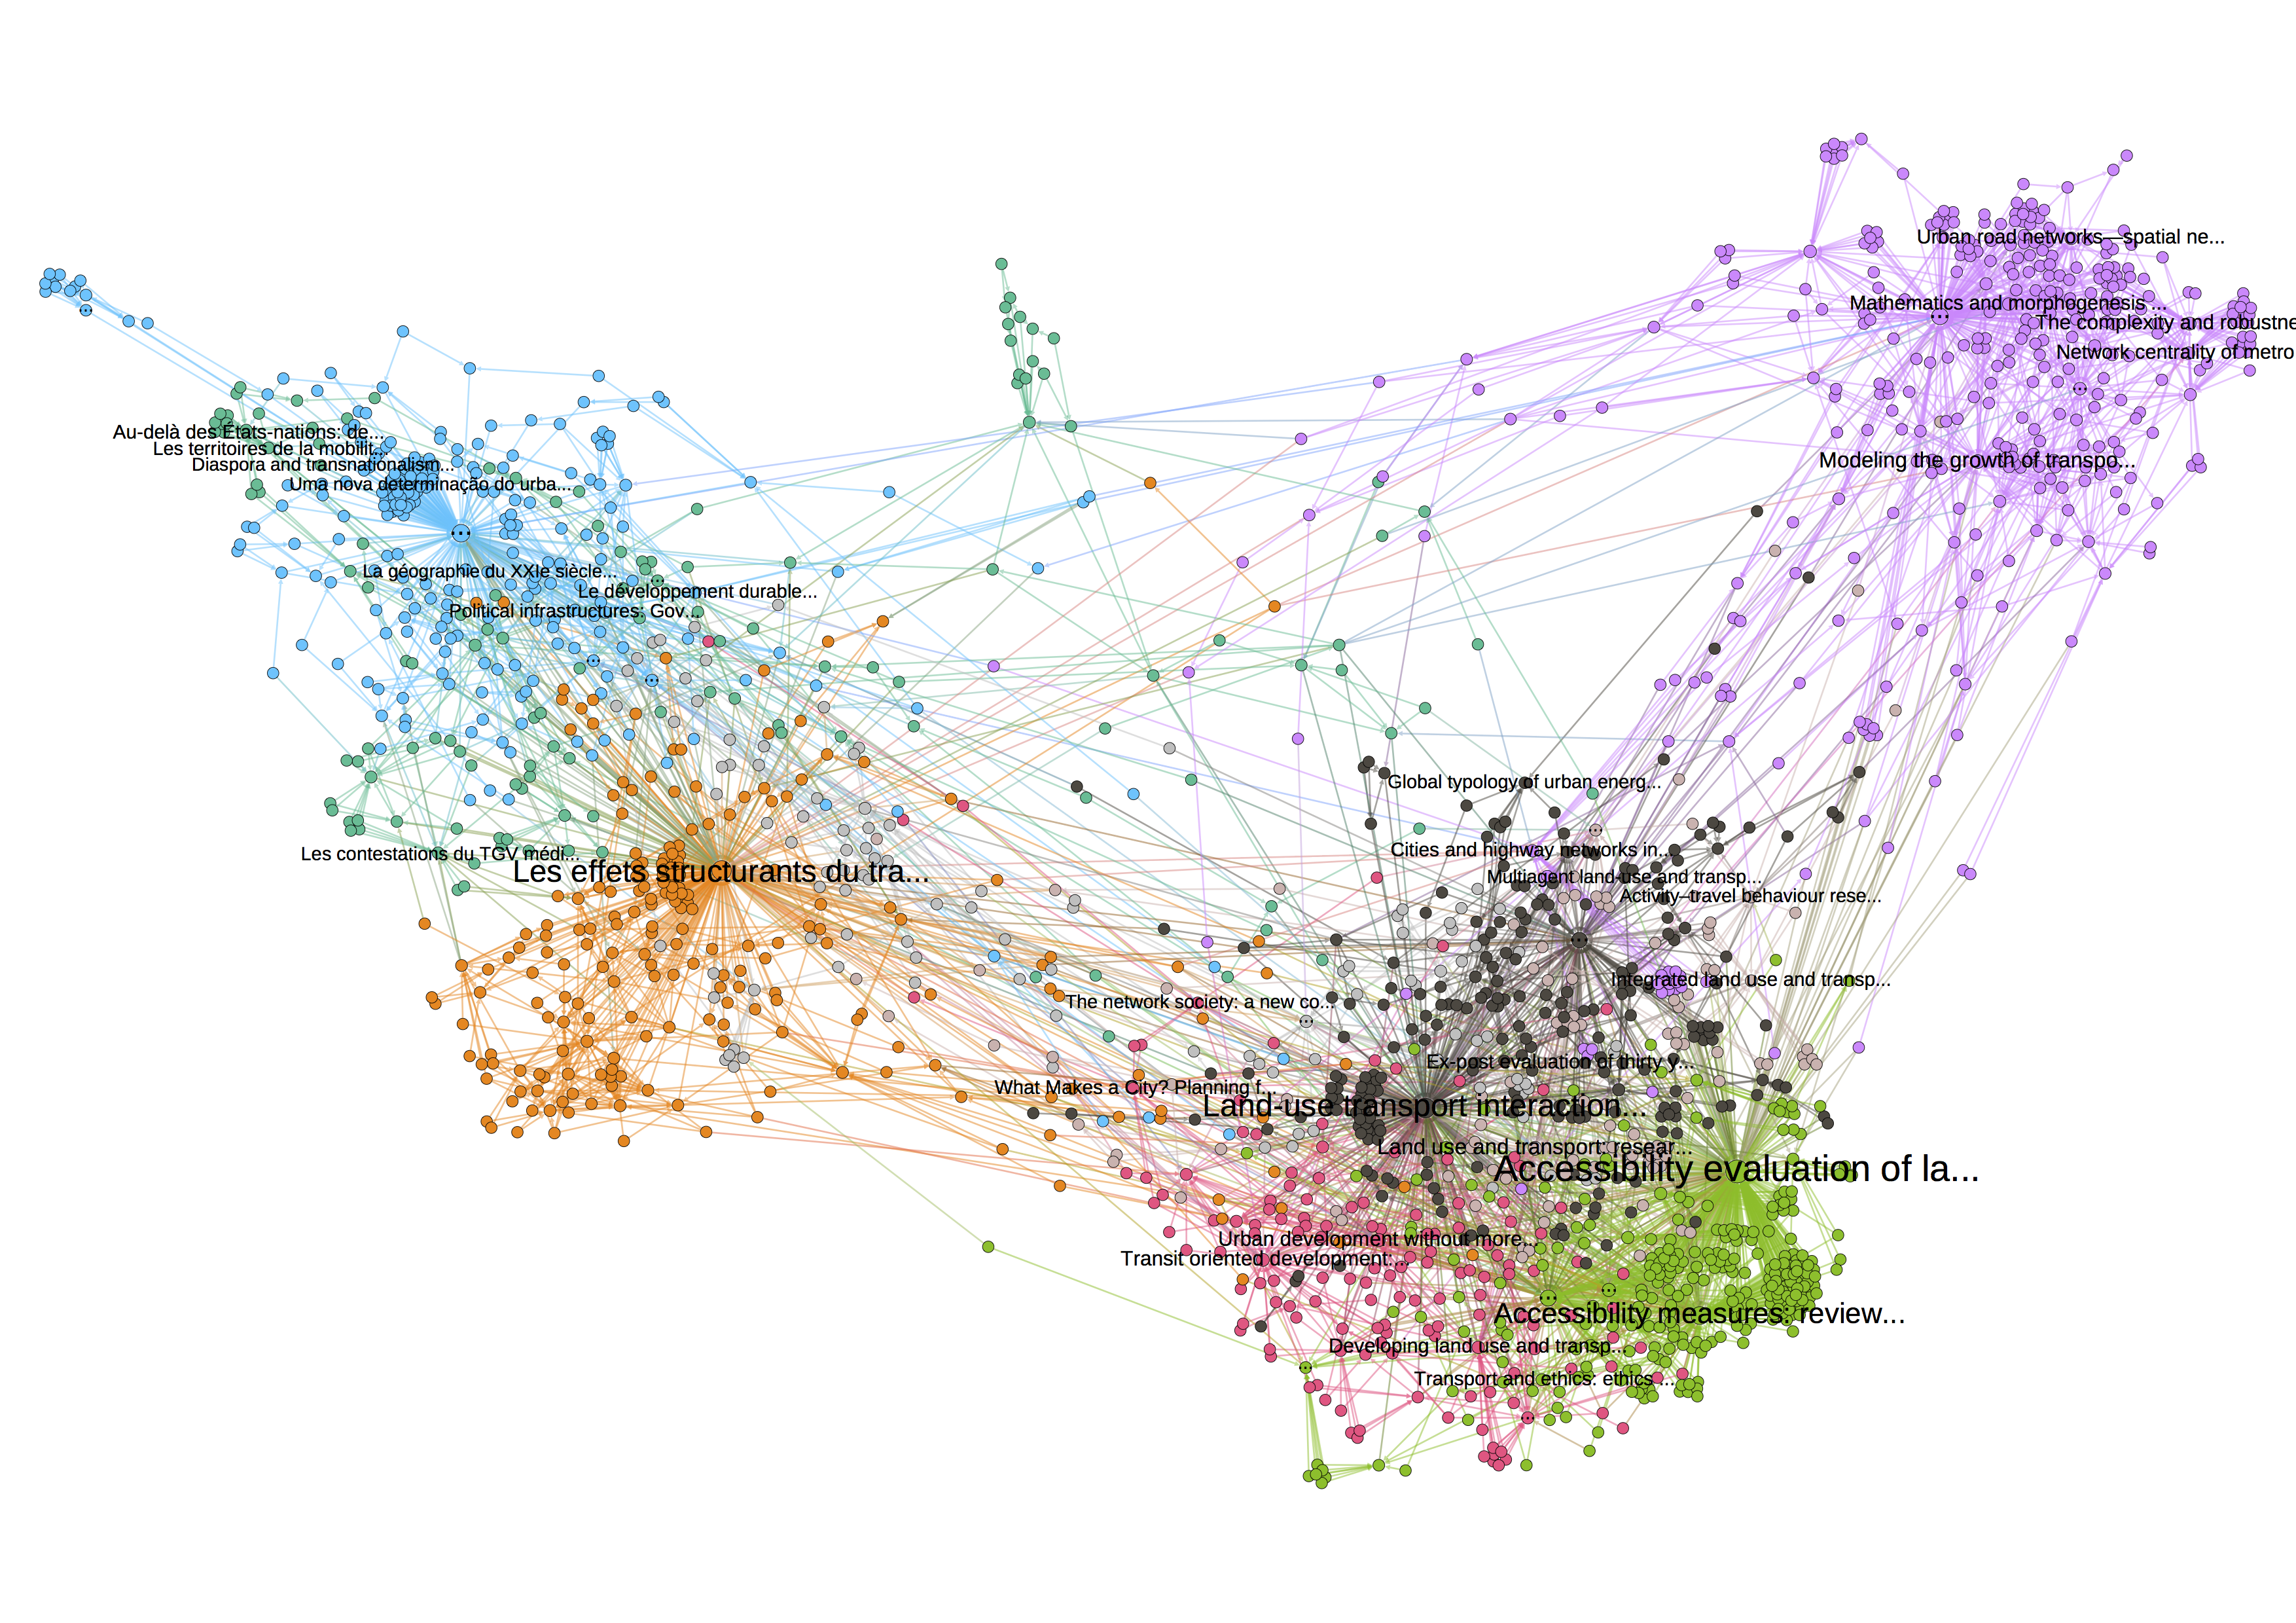
\includegraphics[width=\linewidth]{Figures/QuantEpistemo/rawcore}
\caption[Citation Network][Réseau de citations]{\textbf{Citation Network}\label{fig:quantepistemo:citnw}}{\textbf{Réseau de citations.} Nous visualisons les références ayant au moins deux liens, par un algorithme de force-atlas. Les couleurs donnent les communautés décrites dans le texte. En orange, bleu, turquoise: géographie urbaine, géographie des transports, sciences politiques ; en rose, noir, vert: planning, accessibilité, LUTI ; en violet : réseaux spatiaux (physique et économie).\label{fig:quantepistemo:citnw}}
\end{figure}
%%%%%%%%%%%%%%%%%





%%%%%%%%%%%%%%%%%%
\paragraph{Semantic Communities}{Communautés Sémantiques}


L'extraction des mots-clés est faite suivant une heuristique inspirée de~\cite{chavalarias2013phylomemetic}. La description complète de la méthode et de son implémentation est donnée en Appendice~\ref{app:sec:cybergeo}. Elle se base sur les relations au second ordre entre les entités sémantiques, qui sont des \emph{n-grams}, c'est à dire des mots-clés multiples pouvant avoir une longueur jusqu'à 3. Celles-ci sont estimées via la matrice de co-occurrence, dont les propriétés statistiques fournissent une mesure de déviation à des co-occurrences uniformes, qui est utilisée pour juger la pertinence des mots-clés. Sélectionnant un nombre fixe de mots-clés pertinents $K_W = 10000$, nous pouvons ensuite construire un réseau pondéré par les co-occurrences.


\bpar{
The topology of raw networks does not allow the extraction of clear communities, in particular because of the presence of hubs that correspond to frequent terms common to many fields (e.g. \texttt{model}, \texttt{space}). We assume these highest degree terms do not carry specific information on particular classes and can be thus filtered given a maximal degree threshold $k_{max}$. Similarly, edge with small weight are considered as noise and filtered according to a minimal edge weight threshold $\theta_w$. Keywords are preliminary filtered by a document frequency window $\left[ f_{min},f_{max} \right]$ which is slightly different from network filtering and complementary. A sensitivity analysis of resulting network topology to these parameters is presented in Fig.~\ref{fig:sensitivity}. We choose parameter values that maximize modularity under the constraint of a community number and size distribution of same magnitude as technological classes. This multi-objective optimization does not have a unique solution as objectives are somehow contradictory, and a compromise point must be chosen.
}{
La topologie du réseau brut ne permet pas l'extraction claire de communautés, en particulier à cause de hubs qui correspondent à des termes fréquents commun à de nombreux champs (e.g. \texttt{model}, \texttt{space})\comment[FL]{statut de ces mots ?}. Nous faisons l'hypothèse que ces termes à fort degré ne portent pas d'information particulière sur des classes données et peuvent ainsi être filtrés étant donné un seuil de degré maximal $k_{max}$ (on s'intéresse alors à ce qui fait la spécificité de chaque domaine). De la même manière, les liens avec un poids faibles sont considérés comme du bruit et filtrés selon un seuil de poids minimal $\theta_w$. La méthode générique permet de plus une filtration préliminaire des mot-clés, complémentaire à la filtration topologique, par fréquence d'apparition dans les documents $\left[ f_{min},f_{max} \right]$, à laquelle les résultats ne sont pas sensibles dans notre cas. L'analyse de sensibilité des caractéristiques du réseau filtré, notamment de sa taille, modularité et structure des communautés, est donnée en~\ref{app:sec:quantepistemo}. Nous choisissons des valeurs de paramètres permettant une optimisation multi-objectif entre modularité et taille du réseau, $\theta_w = 10,k_{max} = 500$, par le choix d'un point compromis sur un front de Pareto, qui donne un réseau sémantique de taille $(V=7063,E=48952)$. Celui-ci est visualisé en Appendice~\ref{app:sec:quantepistemo}.
}


\bpar{
We then retrieve communities in the semantic network (using standard Louvain algorithm, with the optimized filtering parameters). communities correspond to well-defined scientific fields (and/or domains, approaches). An expert validation allow us to give names to these, a more complicated naming procedure would eventually be possible (as in~\cite{yang2000improving} for the case of patents 
 where a chi-square test on distribution of documents in classes), but we prefer to stick here to a certain level of supervision. Table~\ref{tab:domains} summarizes the communities 
}{
Nous récupérons ensuite les communautés dans le réseau par un clustering de Louvain standard sur le réseau filtré optimal. On obtient 20 communautés pour une modularité de 0.58. Celles-ci sont examinées à la main pour être nommées, les techniques de désignation automatique~\cite{yang2000improving} n'étant pas assez élaborées et ne font pas la distinction implicite entre champs thématiques et méthodologiques par exemple (en fait entre les domaines de connaissance, voir~\ref{sec:knowledgeframework}) qui est une dimension supplémentaire que nous ne traitons pas ici, mais nécessaire pour avoir des désignations parlantes. Les communautés sont décrites en Table~\ref{tab:quantepistemo:semanticdomains}. On voit tout de suite la complémentarité avec l'approche par citation, puisque se dégagent ici à la fois des sujet d'étude (High Speed Rail, Maritime Networks), des domaines et méthodes (Networks, Remote Sensing, Mobility Data Mining), des domaines thématiques (Policy), des méthodes pures (Agent-based Modeling, Measuring). Ainsi, une référence peut mobiliser plusieurs de ces communautés. On a de plus une granularité plus fine de l'information. L'effet du langage est puissant puisque la géographie française se distingue en une catégorie séparée (des analyses poussées pourraient être envisagées pour mieux comprendre le phénomène et en tirer parti: sous-communautés, reconstruction d'un réseau spécifique, études par traduction ; mais celles-ci sont hors de propos dans cette étude exploratoire). On constante l'importance des réseaux, des problématiques de sciences politiques et socio-économiques. Nous mobiliserons la première catégorie dans la plupart des modèles développés, mais en gardant en tête l'importance des problématiques liées à la gouvernance, nous réaliserons un travail spécifique en~\ref{sec:lutetia}.
}




%%%%%%%%%%%%%%%%%%
\begin{table}
\caption[Semantic communities][Communautés sémantiques]{Disciplines/domains/fields reconstructed from community detection in the semantic network}{\textbf{Description des communautés sémantiques.} On donne leur taille, leur proportion en quantité de mots-clés cumulés sur l'ensemble du corpus, et des mots-clés représentatifs sélectionnés par degré maximal.\comment[FL]{pourquoi ces mots sont ils tronques ?}[(JR) cest explique dans le texte (surtout en annexe) il s'agit de stem]}
\label{tab:quantepistemo:semanticdomains}
\begin{tabular}{llll}
\hline\noalign{\smallskip}
Name & Size & Weight & Keywords  \\
\noalign{\smallskip}\hline\noalign{\smallskip}
Networks & 820 & 13.57\% & \texttt{social network, spatial network, resili} \\
Policy & 700 & 11.8\% & \texttt{actor, decision-mak, societi} \\
Socio-economic & 793 & 11.6\% & \texttt{neighborhood, incom, live} \\
High Speed Rail & 476 & 7.14\% & \texttt{high-spe, corridor, hsr} \\
French Geography & 210 & 6.08\% & \texttt{système, développement, territoire} \\
Education & 374 & 5.43\% & \texttt{school, student, collabor} \\
Climate Change & 411 & 5.42\% & \texttt{mitig, carbon, consumpt} \\
Remote Sensing & 405 & 4.65\% & \texttt{classif, detect, cover} \\
Sustainable Transport & 370 & 4.38\% & \texttt{sustain urban, travel demand, activity-bas} \\
Traffic & 368 & 4.23\% & \texttt{traffic congest, cbd, capit} \\
Maritime Networks & 402 & 4.2\% & \texttt{govern model, seaport, port author} \\
Environment & 289 & 3.79\% & \texttt{ecosystem servic, regul, settlement} \\
Accessibility & 260 & 3.23\% & \texttt{access measur, transport access, urban growth} \\
Agent-based Modeling & 192 & 3.18\% & \texttt{agent-bas, spread, heterogen} \\
Transportation planning & 192 & 3.18\% & \texttt{transport project, option, cba} \\
Mobility Data Mining & 168 & 2.49\% & \texttt{human mobil, movement, mobil phone} \\
Health Geography & 196 & 2.49\% & \texttt{healthcar, inequ, exclus} \\
Freight and Logistics & 239 & 2.06\% & \texttt{freight transport, citi logist, modal} \\
Spanish Geography & 106 & 1.26\% & \texttt{movilidad urbana, criteria, para} \\
Measuring & 166 & 1.0\% & \texttt{score, sampl, metric} \\
\noalign{\smallskip}\hline
\end{tabular}
\end{table}
%%%%%%%%%%%%%%%%%%



%%%%%%%%%%%%%%%%%%
\paragraph{Measures of Interdisciplinarity}{Mesures d'interdisciplinarité}


\bpar{
Distribution of keywords within communities provides an article-level interdisciplinarity.
Combination of citation and semantic layers in the hyper-network provide second order interdisciplinarity measures, that we don't use here because of the modest size of the citation network. More precisely, a reference can be viewed as a probability vector on semantic classes.
}{
La distribution des mots clés dans les communautés permettent de définir une mesure d'interdisciplinarité au niveau de l'article. La combinaison des couches de citation et sémantique dans l'hyperréseau fournit des mesures d'interdisciplinarité au second ordre (motifs sémantiques des cités ou des citants), que nous n'utiliserons pas ici à cause de la taille modeste du réseau de citation (voir \ref{app:sec:cybergeo} et \ref{app:sec:patents}). Plus précisément, une référence $i$ peut être vue comme un vecteur de probabilités sur les classes sémantiques $j$, qu'on notera sous forme matricielle $\mathbf{P}=(p_{ij})$. Celles-ci sont estimées simplement par les proportions de mots-clés classifiés dans chaque classe pour la référence. Une mesure classique d'interdisciplinarité~\cite{bergeaud2017classifying} est alors $I_i = 1 - \sum_j p_{ij}^2$. Soit $\mathbf{A}$ la matrice d'adjacence du réseau de citation, et soit $\mathbf{I}_k$ les matrices de selection des lignes correspondants à la classe $k$ de la classification de citation: $Id\cdot \mathbbm{1}_{c(i)=k}$, telle que $I_k \cdot A \cdot I_{k'}$ donne exactement les citations de $k$ vers $k'$. La proximité de citation entre les communautés de citation est alors définie par $c_{kk'} = \sum \mathbf{I}_k \cdot \mathbf{A} \cdot \mathbf{I}_{k'} /  \sum \mathbf{I}_k \cdot \mathbf{A}$. On définit la proximité sémantique en définissant une matrice de distance entre références par $\mathbf{D} = d_{ii'}=\sqrt{\frac{1}{2}\sum (p_{ij}-p{i'j})^2}$ puis la proximité sémantique par $s_{kk'} = \mathbf{I}_k \cdot \mathbf{D} \cdot \mathbf{I}_{k'} / \sum \mathbf{I}_k \sum \mathbf{I}_{k'}$. Nous montrons en Fig.~\ref{fig:quantepistemo:interdisc} les valeurs de ces différentes mesures, ainsi que la composition sémantique des communautés de citation, pour les classes sémantiques majoritaires. La distribution de $I_i$ montre que les papiers gravitant dans le domaine du LUTI sont les plus interdisciplinaires dans les termes utilisés, ce qui pourrait être lié à leur caractère appliqué. Les autres disciplines sont dans des motifs similaires, à part la géographie et la planification des infrastructures qui présentent des distributions quasi-uniformes, témoignant de l'existence de références très spécialisées dans ces classes. Ce n'est pas nécessairement étonnant vu les sous-champs pointus exhibés (sciences politiques par exemples, et de même les études prospectives type coût-bénéfices sont très étriquées). Ce premier croisement des couches nous confirme les spécificités de chaque champ. Concernant les compositions sémantiques, la plupart agissent comme validation externe vu les classes majoritaires. Le champ le moins concerné par les problème socio-économiques est la planification des infrastructure, ce qui donnera du grain à moudre aux détracteurs de la technocratie. Les questions de changement climatique et durabilité sont relativement bien répartie. Enfin, les ouvrages géographiques concernent en majorité des problèmes de gouvernance. Les matrices de proximité confirment la conclusion de la sous-section précédente en terme de citation, les partages étant très faibles, les plus hautes valeurs étant jusqu'à un quart de la planification vers la géographie et des LUTI vers le TOD (mais pas l'inverse, les relations peuvent être à sens unique). Hors, les proximités sémantiques montrent par exemple que LUTI, TOD, Accessibility et Networks sont proches dans leur termes, ce qui est logique pour les trois premiers, et confirme pour le dernier que les physiciens se basent majoritairement sur les méthodes des ces champs liés au planing pour légitimer leur travaux. La géographie est totalement isolée, sa plus proche voisine étant la planification des infrastructures. Cette étude est très utile pour notre propos, puisqu'elle montre des domaines cloisonnés partageant des termes at donc a priori des problématiques et sujet commun. On ne se parle pas alors qu'on parle des languages pas si lointains, d'où la pertinence accrue de les faire parler d'une commune voie dans nos travaux : nos modèles devront mobiliser des éléments, ontologies et échelles de ces différents champs.
}



%%%%%%%%%%%%%%%%%%
\begin{figure}
\includegraphics[width=0.49\linewidth]{Figures/QuantEpistemo/interdisciplinarities}
\includegraphics[width=0.49\linewidth]{Figures/QuantEpistemo/compo_proportion}\\
\includegraphics[width=0.49\linewidth]{Figures/QuantEpistemo/citation_proximities}
\includegraphics[width=0.49\linewidth]{Figures/QuantEpistemo/semantic_proximities}
\caption[][Motifs d'interdisciplinarité]{\label{fig:quantepistemo:interdisc}}{\textbf{Motifs d'interdisciplinarité.} \textit{(Haut Gauche)} Distribution des $I_i$ par classes de citations ; \textit{(Haut Droite)} Composition sémantiques des classes de citation ; \textit{(Bas Gauche)} Matrice de proximité de citation $c_{kk'}$ entre classes de citations ; \textit{(Bas Droite)} Matrice de proximité sémantique $s_{kk'}$ entre classes de citations.\label{fig:quantepistemo:interdisc}\comment[FL]{tu compares les disciplines entre elles mais pas la facon dont elles attaquent les questions au coeur de ta these. c'est dommage.}[(JR)c'est l'objet de la section suivante]}
\end{figure}
%%%%%%%%%%%%%%%%%%



% bootstrap
%min(corrs);max(corrs);mean(abs(corrs))
% -0.170952  0.5496791  0.08384802
% apply(bcorrs,2,mean)
%       minrho        maxrho    meanabsrho     minrhosup     maxrhosup meanabsrhosup 
%  -0.08792137    0.11690677    0.03137750   -0.17686637    0.68579406    0.11079253 
% apply(bcorrs,2,sd)
%       minrho        maxrho    meanabsrho     minrhosup     maxrhosup meanabsrhosup 
%  0.012683338   0.021324056   0.002250636   0.038402781   0.134996447   0.051553244 

% modularities
% sem : 0.1053156
% cit : 0.8140818
% bootstrap N=100
% sem : 0.073097051446193 +- 0.00307154703966512
% cit : 0.204223565075042 +- 0.0141450119581389


\bpar{
}{
Nous concluons cette analyse par une approche plus robuste pour quantifier les proximités entre couches de l'hyperréseau. Il est aisé de construire une matrice de corrélation entre deux classifications, par les corrélations de leur colonnes. Nous définissons les probabilités $\mathbf{P}_C$ toutes égales à 1 pour la classification de citation. La matrice de correlation de celle-ci avec $\mathbf{P}$ s'étend de -0.17 à 0.54 et a une moyenne de valeur absolue de 0.08, ce qui est significatif par rapport à des classifications aléatoire puisque un bootstrap à $b=100$ répétitions avec les matrices mélangées donne un minimum à $-0.08 \pm 0.012$, un maximum à $0.11 \pm 0.02$ et une moyenne absolue à $0.03 \pm 0.002$. Cela montre que les classifications sont complémentaires et que cette complémentarité est significative statistiquement par rapport à des classifications aléatoires. L'adéquation de la classification sémantique par rapport au réseau de citation peut également être quantifiée par la modularité multi-classes~\cite{nicosia2009extending} (voir~\ref{sec:app:patents} pour une définition mathématique), qui traduit la probabilité qu'un lien soit dû à la classification étudiée, en prenant en compte l'appartenance simultanée à de multiples classes. Ainsi, la modularité multi-classes des probabilités sémantiques pour le réseau de citation est de 0.10, ce qui d'une part est significativement signe d'adéquation, un bootstrap toujours à $b=100$ donnant une valeur de $0.073 \pm 0.003$, qui reste limitée vu la valeur maximale fixée par les probabilités de citations dans leur propre réseau qui donnent une valeur de 0.81, ce qui confirme d'autre part la complémentarité des classifications.
}








%--------------------------------------------------------------



%%%%%%%%%%%%%%%%%%%%%%%%
\subsection{Discussion}{Discussion}




\subsubsection{Towards modeling purpose and context automatic extraction}{Vers une modélisation des thèmes et une extraction automatique du contexte}


\bpar{
A possible direction to strengthen our quantitative epistemological analysis would be to work on full textes related to the modeling of interaction between networks and territories, with the aim to automatically extract thematics within articles. The idea would be to perform some kind of automatized modelography, with possible features to be extracted that would be ontologies, model architecture or structures, scales, or even typical parameter values. It is not clear to what degree structure of models can be extracted from their description in papers and it surely depends on the discipline considered. For example in a framed field such as transportation planning, using a pre-defined ontology (in the sense of dictionary) and a fuzzy grammar could be efficient to extract information as the discipline is relatively formatted. In theoretical and quantitative geography, beyond the barrier of language, information organisation is surely less subject to unsupervised data-mining because of the more literary nature of the discipline : synonyms and figures of speech are generally the norm in good level human sciences writing, fuzzing a possible generic structure of knowledge description. 
}{
Une direction possible pour renforcer cette analyse en épistémologie quantitative serait de travailler sur les textes complets des références contenant des efforts de modélisations des interactions entre réseaux et territoires, avec le but d'extraire automatiquement les thématiques des articles. Des méthodes plus adaptées pour les long texte que celle utilisée ici incluent par exemple l'Allocation Latente de Dirichlet~\cite{blei2003latent}. L'idée serait de procéder à une sorte de modélographie automatique, pour extraire des caractéristiques telle les ontologies, l'architecture ou la structure des modèles, les échelles ou même des valeurs typiques des paramètres. Il n'est pas clair dans quelle mesure la structure des modèles peut être extraite de leur description dans un article, et cela dépend sûrement de la discipline considérée. Par exemple dans champ relativement cadré comme la planification des transports, l'utilisation d'une ontologie pré-définie (dans le sens d'un dictionnaire) et d'une grammaire floue pourrait être efficace vu les conventions assez strictes dans la discipline. En géographie théorique et quantitative, au delà de la barrière du language\comment[FL]{?}, l'organisation de l'information est sûrement plus délicate à appréhender par de l'apprentissage non-supervisé à cause de la nature plus littéraire de la discipline : les synonymes et les figures de style sont généralement la norme pour l'écriture d'un bon niveau en sciences humaines, rendant plus floue une possible structure générique de la description des connaissances.
}


%Depending on extended results of the two previous sections and on thematic requirements (huge need of knowledge on precise models structure, that may appear when trying to construct more specialized operational models), this project may be conducted with more or less investment.




\subsubsection{Reflexivity}{Réflexivité}


\bpar{
The methodology developed here is particularly interesting since it is reflexive, i.e. it can be used on our work itself. Therefore, an other application will be the reflexivity of our thesis : we attend to proceed to similar analysis on our proper bibliography (and possibly its evolution, available via \texttt{git} history), to understand our patterns of knowledge, possible gaps or unveil unexpected developments. The detailed development is done in Appendix~\ref{app:reflexivity}.
}{
La méthodologie que nous avons développé ici est particulièrement intéressante puisqu'elle offre des potentialités de réflexivité, c'est à dire qu'elle peut être utilisée pour étudier notre approche elle-même. Une de ses applications, hors de celle à la revue scientifique Cybergeo dans la perspective de Science Ouverte (voir Appendice~\ref{app:sec:cybergeo}), sera à notre propre corpus de références, dans le but de révéler des possibles  directions de recherche ou problématiques exotiques. Il est éventuellement possible de le faire de manière dynamique, grâce à l'historique de \texttt{git} qui permet de récupérer n'importe quelle version de la bibliographie à une date donnée sur les trois ans écoulés. Il s'agira aussi de comprendre nos motifs de production de connaissance afin de contribuer à~\ref{sec:knowledgeframework}. Le développement détaillé est fait en Appendice~\ref{app:reflexivity}.
}





\stars




%
% 2.3 - Modelography


% -> TODO Systematic Review

\comment[JR]{la modélographie doit logiquement arriver après les études d'épistemo quanti, qui ont permis de donner un aperçu de l'horizon scientifique}



\section{Systematic Review and Modelography}{Revue Systématique et Modélographie}


An ongoing work is the production of a synthesis of this overview, from a modular modeling point of view, combined with a purpose and scale classification. Already mentioned, modular modeling consists in the integration of heterogeneous processes and implementation of processes in order to extract the set of mechanisms giving the best fit to empirical data~\cite{cottineau2015incremental}. We can thus classify models described here according to their building bricks in terms of processes implemented and thus identify possible coupling potentialities. This work is a preliminary step for the analysis in quantitative epistemology developed in chapter~\ref{ch:quantepistemo}.



%%%%%%%%%%%%%%%%%%%%
\subsection[Systematic Review][Revue Systématique]{Systematic Review and Meta-analysis}{Revue systématique et Meta-analyse}


Tandis que les études menées précédemment proposaient de construire un horizon global de l'organisation des disciplines s'intéressant à notre question, nous proposons à présent une étude plus ciblée des caractéristiques de modèles existants. Nous proposons pour cela dans un premier temps une revue systématique, c'est à dire la construction d'un corpus répondant à certaines contraintes, suivie d'une meta-analyse, c'est à dire une tentative d'explication de certaines caractéristiques des modèles par des modèles statistiques.

\comment[JR]{également tenter une classif endogène des modèles : selon les caractéristiques récupérées.}











%%%%%%%%%%%%%%%%%%%%
\subsection{Modelography}{Modélographie}


Nous passons à présent à une analyse qualitative inspirée par les résultats précédents, notamment pour la classification. Elle a pour but d'extraire et de décomposer précisément les ontologies, échelles et processus.














%%%%%%%%%%%%%%%%%%%%
\subsection{Discussion}{Discussion}







%
% Conclusion


%----------------------------------------------------------------------------------------

\newpage

\section*{Synthesis of studied processes}{Synthèse des processus modélisés}



%\paragraph{Synthesis}{Synthèse}

%Nous proposons, pour les modèles identifiés comme incluant la co-évolution, de faire une synthèse des ontologies, des processus, des contextes et des échelles pris en compte.





%%%%%%%%%%%%%
\begin{table}[h!]
\rotatebox{90}{
\begin{tabular}{|l|p{8cm}|p{8cm}|p{8cm}|}
\hline
 & Réseaux $\rightarrow$ Territoires & Territoires $\rightarrow$ Réseaux & Réseaux $\leftrightarrow$ Territoires\\ \hline
Micro & Motifs de mobilité & Congestion du réseau ; Externalités négatives & Mobilité et structure sociale \\ \hline
Meso & Relocalisations ; Effets locaux des infrastructures & Rupture de potentiel & Planification métropolitaine ; TOD \\ \hline
Macro & Interactions entre villes ; Effet tunnel & Différenciation hiérarchique de l'accessibilité & Planification à grande échelle ; Dynamique structurelle ; Bifurcations\\ \hline
\end{tabular}
}
\end{table}
%%%%%%%%%%%%%









%----------------------------------------------------------------------------------------

\newpage


\section*{Chapter Conclusion}{Conclusion du Chapitre}

La réflexivité, au sens de la reflexion de la recherche sur les facteurs influençant son contenu et sa propre structure, semble dans notre cas être nécessaire pour une appréhension claire des enjeux thématiques, méthodologiques et plus généralement scientifiques liés au processus que nous cherchons à modéliser : ceux-ci étant multi-scalaires, hybrides et hétérogènes, les angles d'approches et questionnements possibles sont nécessairement extrêmement variés, complémentaires et riche. Il pourrait s'agir d'une caractéristique fondamentale des systèmes socio-techniques, que \noun{Pumain} formule dans~\cite{pumain2005cumulativite} comme ``une nouvelle mesure de complexité'', qui serait liée aux nombre de point de vue nécessaires pour appréhender un système à un niveau donné d'exhaustivité. Cette idée rejoint la position de \emph{perspectivisme appliqué} que la section~\ref{sec:csframework} formalise et qui est implicitement présente dans l'investigation des relations entre Economie et Géographie développée en~\ref{app:sec:ecogeo}. Ainsi, la modélisation des interactions entre réseaux et territoires peut être reliées à un ensemble très large de disciplines et d'approches revues en section~\ref{sec:modelingsa}. Afin de mieux comprendre le paysage scientifique environnant, et quantifier les rôles ou poids relatifs de chacune, nous avons procédé à une série d'analyse en épistémologie quantitative en~\ref{sec:quantepistemo}. Une première analyse préliminaire basée sur une revue systématique algorithmique suggère un certain cloisonnement des domaines. Cette conclusion est confirmée par l'analyse d'hyperréseau couplant réseau de citation et réseau sémantique, qui permet également de dessiner plus finement les contours disciplinaires, à la fois sur leur relations directes (citations) mais aussi leur proximité scientifique pour les termes et méthodes utilisées. On peut alors utiliser le corpus constitué et cette connaissance des domaines pour une revue systématique semi-automatique et une meta-analyse en~\ref{sec:modelography}, qui permet de constituer un corpus de travaux traitant directement du sujet, qui est ensuite inspecté intégralement, permettant de lier caractéristique des modèles au différents domaines. On a alors à ce stade une idée assez précise de ce qui ce fait, pourquoi et comment. L'enjeu reste de déterminer les pertinences relatives de certaines approches ou ontologies, ce qui sera le but des trois chapitres de la deuxième partie. Nous concluons d'abord cette première partie par un chapitre de discussion~\ref{ch:positioning}, éclairant des points nécessaires à clarifier avant une entrée dans le vif du sujet.






\stars

%%%%%%%%%%%%%%%%%%%%%%%%%%%%%



%%%%%%%%%%%%%%%%%%%%%%%%%%%%%
% Chapter 3 : Positioning



% Chapter 

%\chapter{Positioning}{Positionnements} % Chapter title
\chapter{Positionnements}


\label{ch:positioning} % For referencing the chapter elsewhere, use \autoref{ch:name} 

%----------------------------------------------------------------------------------------

%\headercit{}{}{}

\bigskip


Toute activité de recherche serait, selon certains acteurs de celle-ci, nécessairement politisée, de par pour commencer le choix de ses objets. Ainsi, \noun{Ripoll} alerte contre l'illusion d'une recherche objective et les dangers de la technocratie~\cite{ripoll2017jig}. Nous ne rentrerons pas dans ces débats bien trop vastes pour être traités même en un chapitre, puisqu'il rejoignent des thèmes de sciences politiques, d'éthique, de philosophie, liés par exemple à la gouvernance scientifique, à l'insertion de la science dans la société, à la responsabilité scientifique.


 Il est clair que même des sujets a priori intrinsèquement objectifs, comme la physique des particules et des hautes énergies, ont des implications regardant d'une part les choix de leur financements et les externalités associées (par exemple, l'existence du CERN a largement contribué au développement du calcul distribué), mais d'autre part aussi les applications potentielles des découvertes qui peuvent avoir des répercussions sociales considérables. En biologie, l'éthique est au coeur des principes fondateurs des disciplines, comme en témoignent les débats soulevés par l'émergence de la biologie synthétique~\cite{gutmann2011ethics}. Les tenants d'approche prudentes dans celle-ci se recoupent avec la biologie intégrative, or les sciences intégratives défendues par \noun{Paul Bourgine}, mises en oeuvre par l'intermédiaire du campus digital Unesco CS-DC\footnote{\url{https://www.cs-dc.org/}}, ont typiquement la responsabilité sociale et l'implication citoyenne au coeur de leur cercle vertueux. En sciences humaines et sociales, comme les recherches interagissent avec les objets étudiés (en quelque sorte l'idée des \emph{interactive kind} de \noun{Hacking}~\cite{hacking1999social})%\comment[SR]{num de page et-ou citation en note de bas de page pour définir le concept pour le lecteur, ref plus précise en géographie/sys ville comme ex Batty 1976 ??}
 , les implications politiques et sociales de la recherche sont bien évidemment indiscutables.
 
%Là où il y aurait matière à discussion, et nous y reviendrons en ouverture~\ref{ch:opening} car il s'agira d'une des questions ouvertes posées par notre recherche et sa démarche dans leur ensemble, serait sur la compatibilité des méthodes systématiques et \emph{evidence-based} avec les sciences sociales, autrement dit dans quelle mesure peut-on s'extraire de certains dogmatismes encore plus marqués lors de l'usage de théorie politiques\footnote{\noun{Monod} montre par exemple les désastres liés aux ``niaiseries épistémologiques'' découlant de l'application littérale de la dialectique matérialiste marxiste à l'épistémologie du vivant.}.
   
Nous nous placerons ici à un niveau épistémologique, c'est-à-dire à des réflexions sur la nature et le contenu des connaissances scientifiques au sens large, c'est-à-dire co-construites et validées au sein d'une communauté imposant certains critères de scientificité~\cite{morin1991methode}, bien sûr évolutifs puisque nous nous positionnerons pour la systématisation de certains. Mais donc, même en restant à ce niveau, des prises de positions sont nécessaires, celles-ci pouvant être épistémologiques, méthodologiques, thématiques. Ces dernières ont déjà été ébauchées dans les deux chapitres précédents par les choix des objets d'étude, des problématiques, et seront renforcées à mesure de la progression.
% pour finalement être synthétisées en Chapitre~\ref{ch:theory}.
 
 
Nous proposons ainsi ici un exercice relativement original mais que nous jugeons nécessaire pour une lecture plus fluide de la suite. Il consiste en le développement précis de certains positionnements qui ont une influence particulière dans notre démarche de recherche.

Dans une première section (\ref{sec:computation}), nous précisons notre position au regard des modèles de simulation. Après avoir détaillé les fonctions que nous prêterons aux modèles, nous argumentons sous forme d'essai pour un usage raisonné des données massives et du calcul intensif, et illustrons notre positionnement par rapport à l'exploration des modèles par une étude de cas méthodologique pour l'exploration de la sensibilité des modèles aux conditions initiales.

Dans une deuxième section (\ref{sec:reproducibility}), nous développons des exemples pour illustrer le besoin et la difficulté de reproductibilité, ainsi que les liens avec des nouveaux outils pouvant la favoriser mais aussi la mettre en danger. Nous illustrons la question d'ouverture des données et d'exploration interactive par une étude de cas empirique des flux de trafic en Ile-de-France.

Enfin, la dernière section (\ref{sec:epistemology}) explicite modestement des positions épistémologiques, notamment concernant le courant dans lequel nous nous plaçons, la complexité des objets en sciences sociales, et la nature de la complexité de manière générale.

Le lecteur très familier avec les ``commandements'' de \noun{Banos}~\cite{banos2013pour} pourra trouver dans les deux premières sections des illustrations pratiques originales de ceux-ci, notre positionnement étant principalement dans leur lignée.

%\comment[SR]{Théoreme de l'entonnoir de banos, ne vaudrait il mieux pas partir du plus large et finir sur le plus reserré ? Ce qui permettrait de dire en quoi les deux premières sections actuelles (reproductibilité, calcul) servent un tout plus général (complexité en géo) ?}[plus difficile a lire comme cela]


\stars


\textit{Ce chapitre est composé de divers travaux. La première section est inédite pour ses deux premières parties, et pour sa dernière partie reprend des idées présentées dans \cite{cottineau2017initial}. La deuxième section rend compte pour sa première partie du contenu théorique de \cite{raimbault2016cautious}, et reprend \cite{raimbault2017investigating} pour l'illustration empirique. La troisième section reprend dans sa première partie les bases épistémologiques de \cite{raimbault:halshs-01505084} approfondies par \cite{raimbault2017applied}, est inédite pour sa deuxième partie et rend compte de \cite{raimbault2017complex} pour sa dernière partie.
}







%
% 3.1 Reproducibility and Open Science




%----------------------------------------------------------------------------------------

\newpage

% Section : Reproducibility


\section{Reproducibility}{Reproducibilité}

\label{sec:reproducibility}


%----------------------------------------------------------------------------------------



\bpar{
The strength of science comes from the cumulative and collective nature of research, as progresses are made as Newton said ``standing on the shoulder of giants'', meaning that the scientific enterprise at a given time relies on all the work done before and that advances would not be possible without constructing on it. It includes development of new theories, but also extension, testing or falsifiability of previous ones.
}{
La force de la Science vient de la nature cumulative et collective de la recherche, puisque les progrès sont faits lorsque, comme \noun{Newton} l'a bien posé, on ``se tient sur les épaules de géants'', au sens que l'entreprise scientifique à un temps donné repose sur l'ensemble du travail précédent et qu'aucune avancée ne serait possible sans construire dessus. Cela inclut le développement de nouvelles théories, mais aussi l'extension, le test et la falsification de précédentes: l'avancée dans la construction de la tour signifie aussi la déconstruction de certaines briques obsolètes. Cet aspect de validation par les pairs et de remise en question constante est aussi ce qui légitime la Science pour une connaissance plus robuste et un progrès sociétal basés sur une connaissance d'un univers objectif, par rapport aux systèmes dogmatiques qu'ils soient politiques ou religieux~\cite{bais2010praise}. % note : pourrait introduire Monod ethique de la connaissance, pas le point.
}



\bpar{
The effective practice of reproducibility seems to be increasing~\cite{stodden2010scientific} and technical means to achieve it are always more developed (as e.g. ways to make data openly available, or to be transparent on the research process such as \texttt{git}~\cite{ram2013git}, or to integrate document creation and data analysis such as \texttt{knitr}~\cite{xie2013knitr}), at least in the field of modeling and simulation. However, the devil is indeed in the details and obstacles judged at first sight as minor become rapidly a burden for reproducing and using results obtained in some previous researches. We describe two cases studies where models of simulation are apparently highly reproducible but unveil as puzzles on which research-time balance is significantly under zero, in the sense that trying to exploit their results may cost more time than developing from scratch similar models.
}{
La reproductibilité semble être de plus en plus pratiquée de manière effective~\cite{stodden2010scientific} et les moyens techniques pour l'achever sont toujours plus développés (comme par exemple les outils pour déposer les données ouvertes, ou pour être transparent dans le processus de recherche comme \texttt{git}~\cite{ram2013git}, ou pour intégrer la création de document et l'analyse de données comme  \texttt{knitr}~\cite{xie2013knitr}), au moins dans le champ de la modélisation et de la simulation. Cependant le diable est bien dans les détails et des obstacles jugés dans un premier temps comme mineurs peuvent rapidement devenir un fardeau pour reproduire et utiliser des résultats obtenus dans des recherches précédentes. Nous décrivons deux études de cas où les modèles de simulation sont en apparence hautement reproductibles mais se révèlent vite des puzzles pour lesquels l'équilibre de temps de recherche passe rapidement sous zéro, au sens où essayer d'exploiter leur résultats coûtera plus en temps que de développer entièrement des modèles similaires.
}



%%%%%%%%%%%%%%%%%%%%%%%%%%%%%%%%%%
\subsection{Explicitation, documentation and implementation of models}{Explicitation, documentation et implémentation des modèles}




%%%%%%%%%%%%%%%%%%%%%%%%%%%%%%%%%%
\subsubsection{On the Need to Explicit the Model}{Sur le Besoin d'expliciter le modèle}


\bpar{
A current myth (to which we ourselves struggle to escape indeed) is that providing entire source code and data will be a sufficient condition for reproducibility. It will work if the objective is to produce exactly same plots or statistical analysis, assuming that code provided is the one which was indeed used to produce the given results. It is however not the nature of reproducibility. First, results must be as much implementation-independent as possible for clear robustness purposes. Then, in relation with the precedent point, one of the purposes of reproducibility is the reuse of methods or results as basis or modules for further research (what includes implementation in another language or adaptation of the method), in the sense that reproducibility is not replicability as it must be adaptable~\cite{drummond2009replicability}.
}{
Un mythe à la vie dure (auquel nous essayons en fait nous-même d'échapper) est que fournir le code source complet et les données seront une condition suffisante pour la reproductibilité, puisque la reproductibilité computationnelle complète implique un environnement similaire ce qui devient vite ardu à produire comme le montre~\cite{2016arXiv160806897H}. Pour résoudre ce problème, \cite{10.1371/journal.pone.0152686} propose l'utilisation de conteneurs Dockers qui permet de reproduire même le comportement de logiciels avec interface graphique independemment de l'environnement. C'est d'ailleurs une des direction courantes de développement d'OpenMole, pour simplifier le packaging des bibliothèques et des modèles en binaire (cf. \noun{R. Reuillon} dans~\cite{raimbault2017entretiens}). Dans tous les cas, le reproductibilité a des dimensions supplémentaires, il ne s'agit pas de l'objectif unique qui serait est de produire exactement les mêmes graphes et analyses statistiques, en supposant que le code fournit est celui qui a été effectivement utilisé pour produire les résultats donnés. Tout d'abord, doivent être autant que possible indépendants de l'implémentation (c'est à dire du langage, des bibliothèques, des choix de structures de données et de type de programmation) pour des motifs clairs de robustesse. Ensuite, en relation avec le point précédent, un des buts de la reproductibilité est la réutilisation des méthodes ou résultats comme base ou modules pour une recherche future (ce qui comprend une implémentation dans un autre langage ou une adaptation de la méthode), au sens que la reproductibilité n'est pas la possibilité stricte de répliquer car elle doit être adaptable~\cite{drummond2009replicability}.
}



\bpar{
Our first case study fits exactly that scheme, as it was undoubtedly aimed to be shared with and used by the community since it is a model of simulation provided with the Agent-Based simulation platform NetLogo~\cite{wilensky1999netlogo}. The model is also available online~\cite{de2007netlogo} and is presented as a tool to simulate socio-economic dynamics of low-income residents in a city based on a synthetic urban environment, generated to be close in stylized facts from the real town of Tijuana, Mexico. Beside providing the source code, the model appears to be poorly documented in the literature or in comments and description of the implementation. Comments made thereafter are based on the study of the urban morphogenesis part of the model (setup for the ``residential dynamics'' component) as it is our global context of study%~\cite{raimbault2014vers} % not really citable ?
. In the frame of that study, source code was modified and commented, which last version is available on the repository of the project\footnote{at \texttt{https://github.com/JusteRaimbault/CityNetwork/tree/master/Models/Reproduction/UrbanSuite}}.
}{
Notre premier cas d'étude suit exactement ce schéma, puisqu'il a sans aucun doute été conçu pour être partagé avec la communauté et utilisé, s'agissant d'un modèle de simulation fournit avec la plateforme de modélisation agent NetLogo~\cite{wilensky1999netlogo}. Le modèle est également disponible en ligne~\cite{de2007netlogo} et est présenté comme un outil pour simuler les dynamiques socio-économiques des résidents à bas revenus d'une ville au sein d'un environnement urbain synthétique, généré pour ressembler en terme de faits stylisés à la ville réelle de Tijuana, Mexico. Globalement, le modèle fonctionne de la façon suivante : (i) à partir de centre urbains, une distribution d'usage du sol est générée par modélisation procédurale similaire à \cite{lechner2006procedural}, c'est à dire des routes sont générées de proche en proche selon des règles géométriques et de hiérarchie locales, et un usage du sol ainsi qu'une valeur est attribué en fonction des caractéristique du patch (distance au centre, à la route) ; (ii) dans cet environnement urbain sont simulées des dynamiques résidentielles de migrants, qui cherchent à optimiser une fonction d'utilité dépendant du coût de la vie et de la configuration des autres migrants. A part fournir le code source, le modèle n'est que peu documenté dans la littérature ou dans les commentaires et la description de l'implémentation. Les commentaires qui suivent sont basés sur l'étude de la partie du modèle simulant la morphogenèse urbaine (setup pour la composante ``dynamiques résidentielles'') comme il s'agit de notre contexte global d'étude. Dans le cadre de cette étude, le code source a été modifié et commenté, dont la dernière version est disponible sur le dépôt du projet\footnote{at \texttt{https://github.com/JusteRaimbault/CityNetwork/tree/master/Models/Reproduction/UrbanSuite}}.
}



\paragraph{Rigorous Formalization}{Formalisation Rigoureuse}


\bpar{
An obvious part of model construction is its rigorous formalization in a formal framework distinct from source code. There is of course no universal language to formulate it~\cite{banos2013pour}, and many possibilities are offered by various fields (e.g. UML, DEVS, pure mathematical formulation). No paper nor documentation is provided with the model, apart from the embedded NetLogo documentation, that only thematically describes in natural language the ideas behind each step without developing more and provides information about role of different elements of the interface.
}{
Une partie évidente de la construction d'un modèle est sa formalisation rigoureuse dans un cadre formel distinct du code source. Il n'y a bien sûr aucun langage universel pour le formuler~\cite{banos2013pour}, et de nombreuses possibilités sont offertes par de nombreux champs (e.g. UML, DEVS, formulation mathématique pure), mais l'étape de formalisation précise, qui suit généralement une description plus intuitive donnant les idées et processus dominants (``rationelle''), ne peut pas être sautée. On pourrait se dire que le code source y est équivalent, mais ce n'est pas exactement vrai car on pourrait alors ne plus distinguer certains choix d'implémentation de la structure du modèle. Aucun article ni documentation n'accompagne le modèle ici, au delà de la documentation embarquée NetLogo, qui ne décrit que de manière thématique en langage naturel les idées derrière chaque étape sans plus développer et fournit de l'information sur le rôle des différents éléments de l'interface. Comme ces éléments manquent ici, le modèle n'est guère utilisable tel quel. On pourrait nous objecter ici que la partie que nous étudions est une procédure d'initialisation et non le coeur du modèle : nous maintenons que l'ensemble des procédures doit être également documenté et implémenté avec un soin équivalent, ou pointer vers une référence extérieure dans le cas d'utilisation d'un modèle tiers, comme nous le faisons d'ailleurs pour le couplage effectué en~\ref{sec:computation}.
}



\bpar{
This formulation is a key for it to be understood, reproduced and adapted; but it also avoids implementation biases such as
\begin{itemize}
\item Architecturally dangerous elements: in the model, world context is a torus and agents may ``jump'' in the euclidian representation, what is not acceptable for a 2D projection of real world. To avoid that, many tricky tests and functions were used, including unadvised practices (e.g. dead of agents based on position to avoid them jumping).
\item Lack of internal consistence: the example of the patch variable \texttt{land-value} used to represent different geographical quantities at different steps of the model (morphogenesis and residential dynamics), what becomes an internal inconsistence when both steps are coupled when option \texttt{city-growth?} is activated.
\item Coding errors: in an untyped language such as NetLogo, mixing types may conduct to unexpected runtime errors, what is the case of the patch variable \texttt{transport} in the model (although no error occurs in most of run configurations from the interface, what is more dangerous as the developer thinks implementation is secure). Such problems should be avoided if implementation is done from an exact formal description of the model.
\end{itemize}
}{
Une telle formulation est essentielle pour que le modèle soit compris, reproduit et adapté ; mais elle évite également des biais d'implémentation comme
\begin{itemize}
\item Des éléments architecturaux dangereux : dans le modèle, le contexte du monde est une sphère, ce qui n'est pas raisonnable pour un modèle à l'échelle d'une ville. Les agents peuvent ``sauter'' dans la représentation euclidienne, ce qui n'est pas acceptable pour une projection en deux dimensions du monde réel. Pour éviter cela, de nombreux tests et fonctions subtils sont utilisés, incluant des pratiques déconseillées (e.g. mort d'agents basée sur leur position pour les empêcher de sauter).
\item Manque de cohérence interne : par exemple la variable de patch \texttt{land-value} utilisée pour représenter différentes quantités géographiques à différentes étapes du modèle (morphogenèse et dynamiques résidentielles), ce qui devient une incohérence interne quand les deux étapes sont couplées lorsque l'option permettant de faire croître la ville est activée.
\item Erreur de code : dans un langage non typé comme NetLogo, le mélange des types peut conduire à des erreurs inattendues à l'execution, ou même des \emph{bugs} non détectables directement et alors plus dangereux. C'est le cas de la variable de patch \texttt{transport} dans le modèle (même si aucune erreur ne survient dans la majorité des configurations depuis l'interface, ce qui est plus dangereux comme le développeur pense que l'implémentation est sûre). De tels problèmes devraient être évités si l'implémentation est faite à partir d'une description exacte du modèle.
\end{itemize}
}

\paragraph{Transparent Implementation}{Implémentation Transparente}


\bpar{
A totally transparent implementation is expected, including ergonomics in architecture and coding, but \ldots
}{
Une implémentation totalement transparente doit être attendue, incluant une certaine ergonomie dans l'architecture et le code, mais aussi dans l'interface et la description du comportement attendu du modèle.
}

\paragraph{Expected Model Behavior}{Comportement attendu du modèle}


\bpar{
Whatever the definition, a model can not be reduced to its formulation and/or implementation, as expected model behavior or model usage can be viewed as being part of the model itself. In the frame of \noun{Giere}'s perspectivism~\cite{giere2010scientific}, the definition of model includes the purpose of use but also the agent who aims to use it. Therefore a minimal explication of model behavior and exploration of parameter roles is highly advised to decrease chances of misuses or misinterpretations of it. It includes simple runtime charts that are immediate on the NetLogo platform, but also indicators computations to evaluate outputs of the model. It can also be improved visualizations during runtime and model exploration, such as showed in Fig.~\ref{fig:example_tij_viz}.
}{
Quelle que soit la définition, un modèle ne peut pas être réduit à sa formulation et/ou implémentation, comme le comportement attendu ou l'utilisation du modèle peuvent être vu comme des parties du modèle lui-même. Dans le cadre du perspectivisme de \noun{Giere}~\cite{giere2010scientific}, la définition du modèle inclut le motif de l'utilisation mais aussi l'agent qui vise à l'utiliser. Pour cela une explication minimale du comportement du modèle et une exploration du rôle des paramètres est fortement recommandé pour décroître les chances de mauvais usage ou mauvaises interprétations de celui-ci. Cela inclut des graphe simple obtenus immédiatement à l'exécution sur la plateforme NetLogo, mais aussi un calcul d'indicateurs pour évaluer les sorties du modèle. Il peut aussi s'agir de visualisations améliorée pendant l'execution et l'exploration du modèle, comme le montre la figure~\ref{fig:example_tij_viz}.
}


%%%%%%%%%%%%%%%%%%%%%
\begin{figure}
\centering
\hspace{-2cm}
\includegraphics[width=0.33\textwidth]{Figures/Reproducibility/stdView}
\hfill
\includegraphics[width=0.33\textwidth]{Figures/Reproducibility/ViewRoads}
\hfill
\includegraphics[width=0.33\textwidth]{Figures/Reproducibility/landValues_cityFinished}
\caption[Reproducibility and visualization][Reproductibilité et visualisation]{Example of simple improvement in visualization that can help understanding mechanisms implied in the model. \textit{Left: } Example of original output ; \textit{Middle: } Visualization of main roads (in red) and underlying patches attribution, suggesting possible implementation bias in the use of discretized trace of roads to track their positions ; \textit{Right: }Visualization of land values using a more readable color gradient. This step confirms the hypothesis, through the form of value distribution, that the morphogenesis step is an unnecessary detour to generate a random field for which simple diffusion method should provide similar results, as detailed in the paragraph on implementation.}{\textbf{Exemple d'amélioration simple dans la visualisation qui peut aider à appréhender les mécanismes impliqués par le modèle.} (Gauche) Exemple de sortie originale ; (Centre) Visualisation des routes principales (en rouge) et de l'attribution des patches sous-jacente, qui suggère de possibles biais d'implémentation dans l'utilisation de la trace discrete des routes pour garder trace de leur position ; (Droite) Visualisation des valeurs foncières en utilisant un gradient de couleur plus lisible. Cette étape confirme l'hypothèse, par la forme de la distribution des valeurs, que l'étape de morphogenèse est un détour non-nécessaire pour générer un champ aléatoire pour lequel des simples mécanismes de diffusion devrait fournir des résultats similaires, comme détaillé dans le paragraphe sur l'implémentation. Initialement, l'interface du modèle ne permet pas ces options de visualisation, ces à dire se limite à la première image. On ne peut se rendre compte des processus en jeu pour la morphogenèse, liés aux patches de route et au valeurs foncières se diffusant.}
\label{fig:example_tij_viz}
\end{figure}
%%%%%%%%%%%%%%%%%%%%%



%%%%%%%%%%%%%%%%%%%%%
\subsubsection{On the Need of Exactitude in Model Implementation}{Sur le besoin d'exactitude dans l'implémentation du modèle}


\bpar{
Possible divergences between model description in a paper and the effectively implemented processes may have grave consequences on the final reproducibility. The road network growth model given in~\cite{barthelemy2008modeling} is one example of such a discrepancy. A strict implementation of model mechanisms provide slightly different results than the one presented in the paper, and as source code is not provided we need to test different hypotheses on possible mechanisms added by the programmer (that seems to be a connexion rule to intersections under a certain distance threshold). Lessons that could be possibly drawn from this examples are 
\begin{itemize}
\item the necessity of providing source code
\item the necessity of providing architecture description along with code (if model description is in a langage too far from architectural specifications) in order to identify possible implementation biaises
\item the necessity of performing and detailing explicitly model explorations, that would in that case have helped to identify the implementation bias.
\end{itemize}
}{
Des divergences potentielles entre la description du modèle dans un article et les processus effectivement implémentés peut avoir des conséquences graves sur la reproductibilité finale. Le modèle de croissance du réseau routier donné dans~\cite{barthelemy2008modeling} est un exemple d'une telle discrépance. Une implémentation stricte des mécanismes du modèle produit des résultats légèrement différents de ceux présentés dans le papier, et comme le code source n'est pas fourni nous devrions tester différentes hypothèses sur des mécanismes possibles ajoutés par le programmeur (qui semble être une règle de connexion aux intersections sous un certain seuil de distance). Des leçons qui peuvent éventuellement être tirées de cet exemple, qui rejoignent partiellement mais complètent celle tirées dans l'étude de cas précédente, sont
\begin{itemize}
\item la nécessité de fournir le code source
\item la nécessité de fournir une description de l'architecture en même temps que le code (si la description du modèle est faite dans un langage trop loin de spécification architecturales) afin d'identifier des biais possibles d'implémentation
\item la nécessité de procéder à des explorations explicites du modèle et de les détailler, ce qui dans ce cas aurait permis d'identifier de possibles biais d'implémentation.
\end{itemize}
}



\bpar{
Making the last point mandatory may ensure a limited risk of scientific falsification as it is generally more complicated to fake false exploration results than to effectively explore the model. One could imagine an experiment to test the general behavior of a subset of the scientific community regarding reproducibility, that would consist in the writing of a false modeling paper in the spirit of~\cite{zilsel2015canular}, in which opposite results to the effective results of a given model are provided, without providing model implementation. A first bunch of test would be to test the acceptance of a clearly non-reproducible paper in diverse journals, possibly with a control on textual elements (using or not ``buzz-words'' associated to the journal, etc.). Depending on results, a second experiment may be tested with providing open source code for model implementation but still with false results, to verify if reviewers effectively try to reproduce results when they ask for the code (in reasonable computational power limits of course, HPC being not currently broadly available in Humanities).
}{
Rendre le dernier point obligatoire pourrait assurer un risque limité de falsification puisqu'il est généralement plus compliqué de falsifier des résultats d'exploration plutôt que d'explorer effectivement le modèle. On pourrait imaginer une expérience pour tester le comportement général d'un sous-ensemble de la communauté scientifique au regard de la reproductibilité, qui consisterait en l'écriture d'un faux papier de modélisation dans l'esprit de \cite{zilsel2015canular}, dans lesquels des résultats opposés aux résultats effectifs d'un modèle donné seraient fournis, sans fournir l'implémentation du modèle. Un premier test serait de tester l'acceptation d'un papier clairement non reproductible dans divers journaux, si possible avec un contrôle sur les éléments textuels (par exemple en utilisant ou non des ``buzz-words'' chers au journal). Selon les résultats, une expérience plus poussée serait de fournir l'implémentation open source mais toujours avec des résultats modifiés plus ou moins fortement, afin de tester si les reviewers essayent effectivement de reproduire les résultats quand ils demandent le code (dans des capacités de calcul limitées bien sûr, le HPC n'étant pas encore largement disponibles en sciences sociales). Notre intuition est que les résultats obtenus seraient fortement négatifs, vu les difficultés rencontrées par une exigence de discipline de reproduction indépendante lors de nombreuses relectures, même pour des revues faisant de la reproductibilité une condition \emph{sine qua non} de la publication, les auteurs trouvant des astuces pour se dérober aux contraintes (postuler que des données de simulation ne sont pas des données, ne fournir qu'une version agrégée inutile du jeu de données utilisées, etc. ; nous reviendrons sur le rôle des données plus loin).
}






%%%%%%%%%%%%%%%%%%%%%
\subsection{Interactive Exploration and Production of Results}{Exploration interactive et production des résultats}

L'usage d'applications interactives pour la fouille de données a des avantages non discutables, tel qu'une familiarisation avec la structure des données par une vue d'ensemble qui serait beaucoup plus laborieuse voire impossible autrement. C'est la même idée sous-jacente qui justifie l'interactivité pour l'exploration préliminaire des modèles basé-agent intégrée à des plateformes comme Netlogo~\cite{wilensky1999netlogo} ou Gamma [Cit. gamma]. C'était d'ailleurs un objectif couplé qu'avait initialement~\cite{rey2015plateforme}, c'est à dire une intégration complète de l'exploration fine des modèles et de la production des graphes de sortie ainsi que leur exploration interactive. Comme le rappelle R. Reuillon (Entretien du 11/04/2017, voir \ref{app:data:interview}), la plateforme OpenMole qui devait accueillir cette couche supplémentaire était loin d'être mature à l'époque et ne l'est toujours pas aujourd'hui, puisque l'état de l'art de telles pratiques est en pleine construction et bouleversements réguliers~\cite{holzinger2014knowledge}. Des difficultés au regard de la reproductibilité, qui nous concernent particulièrement ici, sont récurrentes et loin d'être résolues. En effet, il faut bien situer la position de ces outils et méthodes comme une aide cognitive préliminaire\footnote{que nous ne jugeons pas superficielle puisque nous les mobilisons au moins par deux fois par la suite, voir \ref{sec:transportationequilibrium} et \ref{sec:energyprice}}, mais peu souvent comme permettant la production de résultats finaux : lorsque les paramètres ou dimension se multiplient, l'export d'un graphe est bien souvent déconnecté de l'information complète ayant conduit à sa production. De la même manière, l'utilisation de notebooks intégrés tel Jupyter, permettant d'intégrer analyses et rédaction du compte-rendu, peut devenir dangereux car on peut justement revenir sur un script, tester différentes valeurs d'un paramètre, et perdre les valeurs qui avaient produit un graphe donné. L'utilisation de versioning peut être une solution partielle mais souvent lourde. Dans l'idéal, tout logiciel interactif permettant l'export de résultats devrait en même temps exporter un script ou une description exacte et utilisable permettant d'arriver exactement à ce point à partir des données brutes. La plupart des applications d'exploration interactives de données spatio-temporelles sont à ce regard relativement immatures scientifiquement, car même dans le cas où elles sont totalement honnêtes et transparentes sur les analyses présentées à l'utilisateur, ce qui n'est malheureusement pas la règle, les tâtonnements d'exploration progressive ne sont pas reproductibles et la méthode d'extraction de caractéristiques est ainsi relativement aléatoire. En poussant le raisonnement, leur utilisation révélerait plutôt l'aveu d'une faiblesse d'un manque de méthodes systématiques accompagnant la découverte de motifs dans des données spatio-temporelles complexes de manière efficace. De manière très visionnaire, \noun{Banos} avait déjà mis en garde contre ``les dangers de la jungle'' des données dans~\cite{banos2001propos}, quand il souligne très justement que l'exploration interactive doit nécessairement se doubler d'indicateurs locaux adaptés, mais surtout d'outils d'exploration automatisés et de critère d'évaluation des choix faits et des motifs découverts par l'utilisateur. On revient encore à l'idée d'une plateforme intégrée dont OpenMole pourrait être un précurseur. La combinaison des capacités cognitives humaines au traitement machine, notamment pour des problèmes de vision par ordinateur, ouvre des possibilités de découvertes inédites, encore plus via une utilisation collective comme en témoigne le Galaxy Zoo~\cite{2010AEdRv...9a0103R}. Les résultats d'un crowdsourcing de la cognition humaine peuvent rivaliser avec les techniques automatiques les plus avancées comme le montre~\cite{10.1371/journal.pone.0178165} pour l'exemple de la comparaison de cartes spatiales. Ces possibilités ne doivent cependant pas être sur-estimées ou utilisées à mauvais escient, et les questions d'intégration efficiente homme-machine sont d'ailleurs totalement ouvertes. Dans le domaine de la visualisation de l'information géographique, \cite{pfaender2009spatialisation} introduit une sémiologie spécifique visant à favoriser l'exploration de grands jeux de données hétérogènes, et l'expérimente sur une application spécifique : il s'agit d'une avancée considérable vers une plateforme intégrée et une exploration interactive saine et reproductible, les directions d'exploration répondant à des modèles basés sur les sciences cognitives. 






%%%%%%%%%%%%%%%%%%%%%
\subsection{Perspectives}{Perspectives}


\bpar{
Again, reproducibility and transparency is a non-negotiable feature of contemporaneous science, along with Open practices and Open Access. Too much examples (see a very recent one in experimental economics~\cite{camerer2016evaluating}) show in various disciplines the lack of reproducibility of experiments, that is a falsification of previous results or a result in itself. Falsification is a costly practice, and even if necessary~\cite{chavalarias2005nobel}, could be made more efficient through more transparency and direct reproducibility, increase therein the global workflow of science. We develop in parallel of this thesis various tools aimed to ease reproducibility, for which an overview is given in appendix~\ref{app:workflow}.
}{
Encore une fois, la reproductibilité et la transparence sont des éléments essentiels incontournables de la science contemporaine, liés aux pratiques de science ouverte et d'accès ouvert. Beaucoup d'exemples (voir un récent en économie expérimentale dans~\cite{camerer2016evaluating}) dans diverses disciplines montrent le manque de reproductibilité des résultats des expériences, alors que celle ci doit pouvoir conduire à une falsification ou à une confirmation de ces résultats. La falsification est une pratique coûteuse car demandant un certain investissement au détriment de sa propre recherche~\cite{chavalarias2005nobel}. Elle pourrait ainsi être rendue plus efficiente grâce à une transparence augmentée. Des outils spécialement dédiés à une reproductibilité directe, souvent permise par l'ouverture, devraient accroître la performance globale de la science. Mais l'accès ouvert a des impacts bien plus large que la science elle-même : \cite{2015arXiv150607608T} montre un transfert des connaissances scientifiques accru vers la société dans le cas d'articles ouverts, notamment par des intermédiaires comme Wikipedia.
}

Le développement et la systématisation de standards et de bonnes pratiques, de manière conjointe sur les différentes problématiques évoquées, est une condition nécessaire à une rigueur scientifique qui devrait être uniforme au travers de l'ensemble des disciplines existantes. Nous construisons par exemple des exemples d'outils facilitant le flot de production scientifique, ceux-ci étant détaillés en Appendice~\ref{app:workflow}. Par exemple, pour les sciences computationnelles, on a déjà évoqué les potentialités de l'utilisation de \texttt{git} qui s'étendent en fait sans contrainte de disciplines ni de types de recherche si les bonnes adaptations sont introduites. Le suivi précis de l'ensemble des étapes d'un projet, gardé en historique offrant la possibilité de revenir à n'importe laquelle à tout moment, mais aussi de travailler de façon collaborative, plus ou moins parallèlement selon les besoins en utilisant les branches, est un exemple de service fourni par cet outil. Un exemple de bonnes pratiques d'utilisation est donné par~\cite{10.1371/journal.pcbi.1004947}. Plus généralement, les sciences computationnelles nécessitent l'adoption de certains standards et pratiques pour assurer une bonne reproductibilité, et ceux-ci restent majoritairement à développer : \cite{wilson2017good} donne des premières pistes. Concernant la qualité des données, de nombreux efforts sont faits pour introduire des cadres de standardisation des données : par exemple~\cite{10.1371/journal.pone.0178731} décrit un cadre conceptuel visant à guider la résolution de problème récurrent liés à la qualité des données de biodiversité (comme par exemple évaluer des mesures jugeant de l'usage possible d'un jeu de données pour un problème donné).



L'accès aux données est également un point crucial pour la reproductibilité, et sans nous y attarder car cela impliquerait des développements sur la définition, la philosophie, le droit des données etc. qui sont des sujets de recherche en eux-même, nous donnons des perspectives sur les potentiels d'une ouverture systématique des données en recherche. En géographie, les \emph{data paper} sont une pratique inexistante, et la règle est plutôt de garder la main jalousement sur un jeu produit, capitalisant sur le fait d'être le seul à y avoir accès. Il est évident que la qualité et quantité des connaissances produites sera nécessairement plus grande si un jeu de données est publiquement ouvert, puisqu'au moins la même chose sera obtenue, et on peut s'attendre à une prise en main par d'autres domaines, d'autres méthodes, et donc à une plus grande richesse. La fermeture induira plutôt des effets négatifs, comme par exemple du temps perdu à recoder un base vectorielle donnée uniquement sous forme de carte dans un article. L'argument du temps passé comme justification à la fermeture est absurde, puisqu'au contraire, en voyant les données comme une composante à part entière de la connaissance (voir le cadre de connaissances en~\ref{sec:knowledgeframework}), le temps passé doit impliquer plus de citations, donc plus d'utilisation, ce qui passe nécessairement par l'ouverture pour des données. De même, quelle logique, sinon la même absurde de propriété des connaissances, pousse les géographes à insérer un copyright sur l'ensemble de leurs cartes mais aussi leurs figures, jusqu'à un copyright pour un simple histogramme qui s'en serait bien passé si on avait pu l'interroger, honnête de simplicité ? Une expérience de revue induit à réellement s'inquiéter sur la valeur donnée à l'ouverture des données par les auteurs : au bout d'une dizaine d'articles, incluant des journaux affichant comme priorité et pré-requis l'ouverture totale des données et modèles, dont un seul est seulement partiellement ouvert et l'ensemble des autres implique de croire sur parole les résultats présentés (alors qu'un des but de la revue est de contourner les biais cognitifs qu'un ou des humains ont forcément par une validation croisée qui doit se faire sur les résultats bruts et non des interprétations contenant ces biais), il est difficile de croire que des mutations profondes des pratiques ne sont pas nécessaire. Mais en suivant l'adage de Framasoft, ``la route est longue mais la voie est libre'', les perspectives sont nombreuses pour une évolution dont la lenteur n'est pas inéluctable. Le journal Cybergéo, pionnier des pratiques d'ouverture en sciences sociales (première revue entièrement électronique, première revue à lancer une rubrique de \emph{model papers}), lance en 2017 une rubrique \emph{data papers} visant à inciter le développement du partage de données et de l'ouverture en géographie. Il reste des zones grises sur lesquelles il est impossible aujourd'hui d'avoir des perspectives, notamment le droit des données. On peut citer des exemples parmi les études empiriques que nous développons : les données bibliographiques sont obtenues au prix d'une guerre de blocage par Google et un effort considérable pour la gagner ; les données immobilières proviennent d'une base propriétaire achetée avec de l'argent public, et nous pouvons profiter d'un flou du contrat pour les rendre disponibles de manière agrégées avec les résultats ; les données des stations essence proviennent d'une source dont la légalité ne devrait pas être creusée plus, et nous ne pouvons malheureusement pas les rendre disponibles sans prendre de risques - cet aspect n'a cependant jamais fait broncher les reviewers qui n'ont même pas mentionné le manque d'accès aux données. L'ouverture implique un engagement qui fait résolument partie de nos positionnements. C'est la même idée qui soutient la construction de l'application \texttt{CybergeoNetworks}\footnote{\texttt{http://shiny.parisgeo.cnrs.fr/CybergeoNetworks}}, qui couple les outils présentés en~\ref{sec:quantepistemo} avec d'autres approches complémentaires d'analyse de corpus, dans le but d'encourager la réflexivité scientifique, et de mettre cet outil ouvert à la disposition d'éditeurs indépendants, pour s'émanciper de la nouvelle main mise des géants de l'édition qui à la recherche d'un nouveau modèle pour sécuriser leur profits parient sur la vente de meta-contenu et de son analyse. Heureusement, la récente loi numérique en France a gagné le bras de fer contre leur revendication d'un droit exclusif sur la fouille de texte complets.

%inserer lien vers residential dynamics repo ? % NON




%\stars



% 3.2 Big Data, Computation and Model Exploration





%----------------------------------------------------------------------------------------

\newpage



\section{Big Data, Computation and Model Exploration}{Données Massives, Calcul Intensif et Exploration des Modèles}

\label{sec:computation}


%----------------------------------------------------------------------------------------



Nous nous positionnons à présent sur les questions liées à l'utilisation des données massives et du calcul intensif, ce qui induit par extension une réflexion sur les méthodes d'exploration de modèles. Il n'est pas évident que ces nouvelles possibilités soient nécessairement accompagnées de mutations épistémologiques profondes, et nous montrons au contraire que leur utilisation nécessite plus que jamais un dialogue avec la théorie. Implicitement, cette position préfigure le cadre épistémologique pour l'étude des Systèmes Complexes dont nous donnons le contexte à la section suivante~\ref{sec:epistemology} et que nous formalisons en ouverture~\ref{sec:knowledgeframework}.



\subsection{For a cautious use of big data and computation}{Pour un usage raisonné des données massives et de la computation}

\bpar{
The so-called \emph{big data revolution} resides as much in the availability of large datasets of novel and various types as in the always increasing available computational power. Although the \emph{computational shift} (\cite{arthur2015complexity}) is central for a science aware of complexity and is undeniably the basis of future modeling practices in geography as \cite{banos2013pour} points out, we argue that both \emph{data deluge} and \emph{computational potentialities} are dangerous if not framed into a proper theoretical and formal framework. The first may bias research directions towards available datasets (as e.g. numerous twitter mobility studies) with the risk to disconnect from a theoretical background, whereas the second may overshadow preliminaries analytical resolutions essential for a consistent use of simulations. We argue that the conditions for most of results in this thesis are indeed the ones endangered by incautious big-data enthusiasm, concluding that a main challenge for future Geocomputation is a wise integration of novel practices within the existing body of knowledge.
}{
La soi-disante \emph{révolution des données massives} réside autant dans la disponibilité de grands jeux de données de nouveaux types variés, que dans la puissance de calcul potentielle toujours en augmentation. Même si le \emph{tournant computationnel} (\cite{arthur2015complexity}) est central pour une science consciente de la complexité et est sans douter la base des pratiques de modélisation futures en géographie comme \cite{banos2013pour} souligne, nous soutenons que à la fois le \emph{déluge de données} et les \emph{capacités de calcul} sont dangereuses si non cadrées dans un cadre théorique et formel propre. Le premier peut biaiser les directions de recherche vers les jeux de données disponibles %(comme par exemple les nombreuses étude de mobilité se basant sur twitter) % TODO find less rude examples, and of different types ?
 avec le risque de se déconnecter d'un fond théorique, tandis que le second peut occulter des résolutions analytiques préliminaires essentielles pour un usage cohérent des simulations. Nous avançons que les conditions pour la majorité des résultats dans cette thèse sont en effet ceux mis en danger par un enthousiasme inconsidéré pour les données massives, tirant la conclusion qu'un challenge majeur pour la géocomputation future est une intégration sage des nouvelles pratiques au sein du corpus existant de connaissances.
}


\bpar{
The computational power available seems to follow an exponential trend, as some kind of Moore's law. Both effective Moore's law for hardware, and improvement of softwares and algorithms, combined with a democratization of access to large scale simulation facilities, makes always more and more CPU time available for the social scientist (and to the scientist in general but this shift happened quite before in other fields, as e.g. CERN is leading in cloud computing and grid computation). About 10 years ago, \cite{gleyze2005vulnerabilite} concluded that network analysis, for the case of Parisian public transportation network, was ``limited by computation''. Today most of these analyses would be quickly done on a personal computer with appropriated software and coding: \cite{2015arXiv151201268L} is a witness of such a progress, introducing new indicators with a higher computational complexity, computed on larger networks. The same parallel can be done for the Simpop models: the first Simpop models at the beginning of the millenium~\cite{sanders1997simpop} were ``calibrated'' by hand, whereas \cite{cottineau2015modular} calibrates the multi-modeling Marius model and~\cite{schmitt2014half} calibrates very precisely the SimpopLocal model, both on grid with billions of simulations. A last example, the field of Space Syntax, witnessed a long path and tremendous progresses from its theoretical origins~\cite{hillier1989social} to recent large-scale applications~\cite{hillier2016fourth}.
}{
La puissance de calcul disponible semble suivre un tendance exponentielle, comme une sorte de loi de Moore. Grace à d'une part la loi de Moore effective pour le matériel, d'autre part l'amélioration des logiciels et algorithmes, conjointement avec une démocratisation de l'accès au infrastructures de simulation à grande échelle, permet à toujours plus de temps processeur d'être disponible pour le chercheur en sciences sociales (et pour le scientifique en général, mais cette mutation a déjà été opérée depuis plus longtemps dans d'autres domaines, puisque par exemple le CERN est à la pointe en terme de calcul distant et sur grille). Il y a environ une dizaine d'année, \cite{gleyze2005vulnerabilite} était forcé de conclure que les analyses de réseau, pour les transports publics parisiens, étaient ``limitées par le calcul''. Aujourd'hui la plupart des mêmes analyses seraient rapidement réglée sur un ordinateur personnel avec les logiciels et programmes appropriés : \cite{2015arXiv151201268L} est un témoin d'un tel progrès, introduisant des nouveaux indicateurs avec une plus grande complexité de calcul, qui sont calculés sur des réseaux à grande échelle. Le même parallèle peut être fait pour les modèles Simpop : les premiers modèles Simpop au début du millénaire~\cite{sanders1997simpop} étaient ``calibrés'' à la main, tandis que \cite{cottineau2015modular} calibre le modèle Marius en multi-modélisation et~\cite{schmitt2014half} calibre très précisément le modèle SimpopLocal, chacun sur la grille avec des milliards de simulations. Un dernier exemple, le champ de la \emph{Space Syntax}, a témoigné d'une longue route et de progrès considérables depuis ses origines théoriques~\cite{hillier1989social} jusqu'à ses récentes applications à grande échelle~\cite{hillier2016fourth}.
}



\bpar{
Concerning the new and ``big'' data available, it is clear that always larger dataset are available and always newer type of data are available. Numerous examples of fields of application can be given. For example, mobility can now be studied from various entries, such as new data from smart transportation systems~\cite{o2014mining}, from social networks~\cite{frank2014constructing}, or other more exotic data such as mobile phone data~\cite{de2016death}. In an other spirit, the opening of ``classic'' datasets (such as city dashboards, open data government initiatives) should allow ever more meta-analyses. New ways to do research and produce data are also raising, towards more interactive and crowd-sourced initiatives. For example, \cite{2016arXiv160606162C} describes a web-application aimed at presenting a meta-analysis of Zipf's law across numerous datasets, but in particular features an upload option, where the user can upload its own dataset and add it to the meta-analysis. Other applications allow interactive exploration of scientific literature for a better knowledge of a complex scientific landscape, as~\cite{cybergeo20} does.
}{
Concernant les nouvelles données ``massives'' qui sont disponibles, il est clair que des quantités toujours plus grandes et des types toujours nouveaux sont disponibles. De nombreux exemples de champs d'application peuvent être donnés. La mobilité en est typique, puisque étudiée selon divers points de vue, comme les nouvelles données issues des systèmes de transport intelligents~\cite{o2014mining}, des réseaux sociaux~\cite{frank2014constructing}, ou des données plus exotiques comme des données de téléphonie mobile~\cite{de2016death}. Dans un autre esprit, l'ouverture de jeux de données ``classiques'' (comme les applications synthétiques urbaines, les initiatives gouvernementales pour les données ouvertes) devrait pouvoir toujours plus de méta-analyses. De nouvelles façon de pratiquer la recherche et produire des données sont également en train d'émerger, vers des initiatives plus interactives et venant de l'utilisateur. Ainsi, \cite{2016arXiv160606162C} décrit une application web ayant pour but de présenter une méta-analyse de la loi de Zipf sur de nombreux jeux de données, mais en particulier inclut une option de dépôt, à travers laquelle l'utilisateur peut télécharger sont propre jeu de données et l'inclure dans la méta-analyse. D'autres applications permettent l'exploration interactive de la littérature scientifique pour une meilleure connaissance d'un horizon scientifique complexe, comme~\cite{cybergeo20} fait.
}


\bpar{
As always the picture is naturally not as bright as it seems to be at first sight, and the green grass that we try to go eating in the neighbor's field quickly turns into a sad reality. Indeed, the purpose and motivation are fuzzy and one can get lost. Some examples speaks for themselves. \cite{barthelemy2013self} introduces a new dataset and rather new methods to quantify road network evolution, but the results, on which the authors seem to be astonished, are that a transition occurred in Paris at the Haussmann period. Any historian of urbanism would be puzzled by the exact purpose of the paper, as in the end a vague and bizarre feeling of reinventing the wheel floats in the air. The use of computation can also be exaggerated, and in the case of agent-based modeling it can be illustrated by the example of~\cite{axtell2016120}, for which the aim at simulating the system at scale 1:1 seems to be far from initial motivations and justifications for agent-based modeling, and may even give arguments to mainstream economists that denigrate easily ABMS. Other anecdotes raise worries: \cite{robin_cura_2014_11415} is a web application that wastes computational ressources to simulate Gaussian distributions for a Gibrat model in order to compute their mean and variance, that are input parameters of the model. It basically checks the Central Limit Theorem, which is a priori well accepted among most scientists. Otherwise, the full distribution given by a Gibrat model is theoretically known as it was fully solved e.g. by \cite{gabaix1999zipf}. Recently on the French speaking diffusion list \emph{Geotamtam}, a sudden rush around \emph{Pokemon Go} data seemed to answer more to an urgent unexplained need to exploit this new data source before anyone else rather than an elaborated theoretical construction. Simple existing accurate datasets, such as historical cities population (for France the Pumain-INED database for example), are far from being fully exploited and it may be more important to focus on these already existing classic data. One must also be aware of the possible misleading applications of some results: \cite{louail2016crowdsourcing} makes a very good analysis of potential redistribution of bank card transactions within a city, but pushes the results as possible basis for social equity policy recommandation by acting on mobility, forgetting that urban form and function are coupled in a complex way and that moving transactions from one place to the other involves far more complex processes than policies.
}{
Comme toujours la situation n'est naturellement pas aussi idyllique qu'elle semble être au premier abord, et l'herbe verte du pré du voisin que nous pouvons être tentés d'aller brouter se transforme rapidement en un triste fumier. En effet, les objectifs et motivations sont flous et on peut facilement s'y perdre. Des illustrations parleront d'elles-même. \cite{barthelemy2013self} introduit un nouveau jeu de données et des méthodes relativement nouvelles pour quantifier l'évolution du réseau de rues, mais les résultats, sur lesquels les auteurs semblent s'étonner, sont qu'une transition a eu lieu à Paris à l'époque d'Haussmann. Tout historien de l'urbanisme s'interrogerait sur le but exact de l'étude, puisque à la fin un sentiment étrange de réinvention de la roue flotte dans l'air. L'utilisation des ressources de calcul peut également être exagéré, et dans le cas de la modélisation multi-agent, on peut citer~\cite{axtell2016120}, pour lequel l'objectif de simuler le système à l'échelle 1:1 semble être loin des motivations et justifications originelles de la modélisation agent, et pourrait même donner des arguments aux économistes \emph{mainstream} qui dénigrent facilement les ABMS. D'autres anecdotes peuvent inquiéter :  il existe en ligne des exemples sidérants, comme une application web\footnote{} qui gâche des ressources de calcul financées par l'argent public pour simuler des distributions Gaussiennes afin de calculer pour un modèle de Gibrat, afin de calculer leur moyenne et variance, qui sont des paramètres d'entrée du modèle. En résumé, cela revient à vérifier le Théorème de la Limite Centrale. D'autre part, la distribution complète donnée par un modèle de Gibrat est entièrement connue théoriquement comme résolu e.g. par~\cite{gabaix1999zipf}. Récemment, sur la liste de diffusion de géographie francophone \emph{Geotamtam}, un soudain engouement autour des données issues de \emph{Pokemon Go} a semblé répondre plus à un besoin urgent et inexpliqué d'exploiter cette source de données avant tous les autres, plutôt qu'à des considérations théoriques élaborées. Des jeux de données existant et précis, comme la population historiques des villes (pour la France la base Pumain-INED par exemple), sont loin d'être entièrement exploités et il pourrait être plus pertinent de se concentrer sur ces jeux de données classiques qui existent déjà. De même, il faut être conscient des possibles applications de résultats basée sur des malentendus : \cite{louail2016crowdsourcing} analyse la redistribution potentielle des transactions de carte bancaire au sein d'une ville, mais présente les résultats comme la base possible de recommandations de politiques pour une équité sociale en agissant sur la mobilité, oubliant que la forme et les fonctions urbaines sont couplés de manière complexe et que déplacer des transactions d'un endroit à un autre implique des processus bien plus complexes que des régulations directes, qui d'autant plus ne s'appliquent jamais de la façon prévue et conduisent à des résultats un peu différents. Une telle attitude, souvent observée de la part de physiciens, est très bien mise en allégorie par la figure~\ref{fig:computation:xkcd} qui n'est qu'à moitié une exagération de certaines situations.
}




\bpar{
Our main claim here is that the computational shift and simulation practices will be central in geography, but may also be dangerous, for the reasons illustrated above, i.e. that data deluge may impose research subjects and elude theory, and that computation may elude model construction and solving. A stronger link is required between computational practices, computer science, mathematics, statistics and theoretical geography. Theoretical and Quantitative Geography is at the center of this dynamic, as it was its initial purpose that seems forgotten in some cases. It implies the need for elaborated theories integrated with conscious simulation practices. In other words we can answer complementary naive questions that have however to be tackled one and for once. If a theory-free quantitative geography would be possible, the answer if naturally no as it is close to the trap of black-box data-mining analysis. Whatever is done in that case, the results will have a very poor explanatory power, as they can exhibit relations but not reconstruct processes. On an other hand, the possibility of a purely computational quantitative geography is a dangerous vision: even gaining three orders of magnitudes in computational power does not solve the dimensionality curse. In our work here, without theory, we would not know which objects, measures and properties to look at (e.g. multi-scale and dynamical nature of processes), and without analytics, it would be sometimes difficult to draw conclusions from empirical analysis. Nothing is really new here but this position has to be stated and stood up, precisely because our work will use this kind of tools, trying to advance on a thin and fragile edge, with the void of the unfunded theoretical charlatanism on one side and the abyss of the technocratic blind drowning in foolish amounts of data. More than ever we need simple but powerful and funded theories {\`a}-la-Occam~\cite{batty2016theoretical}, to allow a wise integration of new techniques into existing knowledge.
}{
Notre principal argument est que le tournant computationnel et les pratiques de simulation seront centrales en géographie, mais peuvent également être dangereux, pour les raisons illustrées ci-dessus, i.e. que le déluge de données peut imposer les sujets de recherche et occulter la théorie, et que la computation peut éluder la construction et la résolution de modèles. Un lien plus fort est nécessaire entre les pratiques de calcul, l'informatique, les mathématiques, les statistiques et la géographie théorique. La Géographie Théorique et Quantitative est au centre de cette dynamique, puisqu'il s'agit de sa motivation initiale principale qui semble oubliée dans certains cas. Cela implique un besoin de recherche de théorie élaborées intégrées avec des pratiques de simulation conscientes. En d'autres mots, on peut répondre à des questions naïves complémentaires qui ont toutefois besoin d'être traitées une bonne fois pour toutes. Si une géographie quantitative libérée de la théorie serait possible, la réponse est naturellement non puisque cela se rapproche du piège de la fouille de données par boîte noire. Quoi qu'il soit fait par cette approche, les résultats auront un pouvoir explicatif très faible, puisqu'ils pourront mettre en valeur des relations mais pas reconstruire des processus. D'autre part, la possibilité d'une géographie quantitative purement basée sur le calcul est une vision dangereuse : même le gain de trois ordres de grandeur dans la puissance de calcul disponible ne résout pas le sort de la dimension. Dans notre travail ici l'absence de théorie impliquerait de ne pas connaitre les objets, mesures et propriétés à étudier (e.g. le caractère multi-scalaire ou dynamique des processus), et sans résolutions analytiques, il serait souvent difficile de tirer des conclusions à partir des analyses empiriques. Rien n'est vraiment nouveau ici mais cette position doit être affirmée et tenue, précisément car notre travail se base sur ce type d'outils, essayant d'avancer sur une arête fine et fragile, avec d'un côté le vide du charlatanisme théorique infondé et de l'autre l'abîme de l'overdose technocratique dans des quantités de données folles. Plus que jamais on a besoin de théories simples mais fondées et puissantes {\`a}-la-Occam~\cite{batty2016theoretical}, pour permettre une intégration saine des nouvelles techniques au sein des connaissances existantes.
}


 
% multi-modeling and model families (see Cottineau, Rey and Reuillon presentation) as one way to do that ?

% Interdisciplinarity (and Nexus ?!) necessary to achieve that.



\comment[JR]{develop the case study presented at RGS, briefly, to illustrate both big data and dependency of computation, analytics and theory ?}




%%%%%%%%%%%%%%
\begin{figure}
\centering
\includegraphics[width=\textwidth]{Figures/Computation/here_to_help}
\caption{}{De l'usage naïf de la fouille de données et du calcul intensif. Source: \texttt{xkcd}}
\label{fig:computation:xkcd}
\end{figure}
%%%%%%%%%%%%%%








%----------------------------------------------------------------------------------------


%  section : synthetic data control - introduces rochebrune paper, feasible correlation space etc, and forthcoming applications ?


\subsection{Statistical Control on Initial Conditions by Synthetic Data Generation}{Contrôle statistique pour les conditions initiales par génération de données synthétiques}

\subsubsection{Context}{Contexte}


\bpar{
When evaluating data-driven models, or even more simple partially data-driven models involving simplified parametrization, an unavoidable issue is the lack of control on ``underlying system parameters'' (what is a ill-defined notion but should be seen in our sense as parameters governing system dynamics). Indeed, a statistics extracted from running the model on enough different datasets can become strongly biased by the presence of confounding in the underlying real data, as it is impossible to know if result is due to processes the model tries to translate or to a hidden structure common to all data.
}{
Lors de l'évaluation de modèle basés sur les données, \comment{(Florent)  data driven models : sens de cette expression ?} ou même de modèle plus simples partiellement basés sur les données impliquant une paramétrisation simplifiée, une issue inévitable est le manque de contrôle sur les ``paramètres implicites du systèmes'' (ce qui n'est pas une notion stricte mais doit être vu dans notre sens comme les paramètres régissant la dynamique). En effet, une statistique issue d'executions du modèle sur un nombre suffisamment grand de jeu de données peut devenir fortement biaisé par la présence de \emph{confunding} dans les données réelles sous-jacentes, comme il est impossible de savoir si les résultats sont dus aux processus que le modèle cherche à traduire ou à une structure commune à toutes les données.
\comment{(Florent) a quelle question cherches-tu ici à répondre ?}
}


%Let illustrate the issue with a simple example.

We formalize briefly a proposition of method that would allow to add controls on meta-parameters, in the sense of parameters driving the represented system at a higher temporal and spatial scale, for a model of simulation. We make the hypothesis that such method is valid under constraints of disjonction for scales and/or ontologies between the model of simulation and the domain of meta-parameters.


\subsubsection{Description}{Description}

An advanced knowledge of the behavior of computational models on their parameter space is a necessary condition for deductions of thematic conclusions \comment{(Florent) pas nécessaire si les comportements sont bien calibrés par des observations dans le monde réel, il n'est pas besoin d'une compréhension si fine du modèle}
 or their practical application~\cite{banos2013pour}. But the choice of varying parameters is always subjective, as some may be fixed by a real-world parametrization, or other may be interpreted as arbitrarily fixed initial conditions. It raises methodological and epistemological issues for the sensitivity analysis, as the scope of the model may become ill-defined. \comment{(Florent) sens ?}

Let consider the concrete example of the Schelling Segregation model~\cite{schelling1971dynamic}. \comment{(Florent) Schelling hors sujet ?}
One of its crucial features on which the literature has been rather controversial is the influence of the spatial structure of the container on which agents evolve.%~(\textit{Biblio Marion}). 
 The thematic aim of the project developed in~\cite{cottineau2015revisiting} is to clarify this point through a systematic model exploration. A methodological contribution is the construction of a framework allowing the analysis of the sensitivity of models to \emph{meta-parameters}, i.e. to parameters considered as fixed initial conditions (e.g. the spatial structure for the Schelling model), or to parameters of another model generating an initial configuration%, as detailed in Fig.~\ref{} \textit{[insert scheme describing the approach]}, 
 yielding thus a \emph{simple coupling} between models (serial coupling). The benefits of such an approach are various but include for example the knowledge of model behavior in an extended frame, the possibility of statistical control when regressing model outputs, a finer exploration of model derivatives than with a naive approach. Some remarks can be made on the approach :
\begin{itemize}
\item What knowledge are brought by adding the upstream model, rather than for example in the Schelling case exploring a large set of initial geometries ? 

$\rightarrow$ \textit{to obtain a sufficiently large set of initial configuration, one quickly needs a model to generate them ; in that case a quasi-random generation followed by a filtering on morphological constraint will be a morphogenesis model, which parameters are the ones of the generation and the filtering methods. Furthermore, as detailed further, the determination of the derivative of the downstream model is made possible by the coupling and knowledge of the upstream model.}
\comment{(Florent) est-ce important pour la thèse ?}


\item Statistical noise is added by coupling models

$\rightarrow$ \textit{Repetitions needed for convergence are indeed larger as the final expectance has to be determined by repeating on the first times the second model ; but it is exactly the same as exploring directly many configuration, to obtain statistical robustness in that case one must repeat on similar configurations.}

\item Complexity is added by coupling models

% check Varenne citation
$\rightarrow$ \textit{In the sense of Varenne~\cite{varenne2010framework} , coupling is simple and no complexity is thus added.}
\end{itemize}
 
%\paragraph{Context}

%Let $M_{m}$ a stochastic model of simulation, which inputs are to simplify initial conditions $D_0$ and parameters $\vec{\alpha}$, and output $M_{m}\left[\vec{\alpha},D_0\right](t)$ at a given time $t$. We assume that it is partially data-driven in the sense that $D_0$ is supposed to represent a real situation at a given time, and model performance is measured by the distance of its output at final time to the real situation at the corresponding time, i.e. error function is of the form $\norm{\Eb{\vec{g}(M_{m}\left[\vec{\alpha},D_0\right](t_f))}-\vec{g}(D_f)}$ where $\vec{g}$ is a deterministic field corresponding to given indicators.

%\paragraph{Position of the Problem}

%Evaluating the model on real data is rapidly limited in control possibilities, being restricted to the search of datasets allowing natural control groups. Furthermore, statistical behaviors are generally poorly characterized because of the small number of realizations. Working with synthetic data first allows to solve this issue of robustness of statistics, and then gives possibilities of control on some ``meta-parameters'' in the sense described before.




%%%%%%%%%%%%%%%%%%%%
\subsubsection{Formal Description}{Description Formelle}

%\subsubsection{Deterministic Formulation}

One has the composition of the derivative along the meta-parameter

\[
\partial_{\alpha}\left[M_u \circ M_d\right] = \left(\partial_{\alpha} M_u \circ M_d \right)\cdot \partial_{\alpha} M_d
\]

$\rightarrow$ \textit{the sensitivity of the downstream model (Schelling) can be determined by studying the serial coupling and the upstream model ; thematic knowledge : sensitivity to an implicit meta-parameter ; and computational gain : generation of controlled differentiates in the ``initial space'' is quasi impossible.}

%\subsubsection{Stochasticity}

The question of stochasticity in simply coupled models causes no additional issue as $\Eb{X}=\Eb{\Eb{X|Y}}$. It naturally multiplies the number of repetition needed for convergence what is the expected behavior.







%%%%%%%%%%%%%%%%%%%%
\subsection{Link between modeling and Open Science}{Lien entre modélisation et Science Ouverte}















%
% 3.3 Epistemological positioning



%----------------------------------------------------------------------------------------


\newpage



\section{Epistemological Positioning}{Positionnement Epistémologique}\label{sec:epistemology}

%----------------------------------------------------------------------------------------



%%%%%%%%%%%%%%%%%%%%%%
\subsection{Cognitive Approach and Perspectivism}{Approche cognitive et Perspectivisme}


\comment[JR]{Pour une science anarchiste (Feyerabend) ; compatibilité avec le Perspectivisme de Giere et pourquoi celui-ci est particulièrement adapté aux paradigmes de la complexité ; multiplicité des lectures de la thèse (voir annexe réflexivité, au delà d'une lecture linéaire)}




%%%%%%%%%%%%%%%%%%%%%%
\subsection{From Life to Culture}{De la Vie à la Culture}
% De Monod à ?
% Le Démon de ? (ref Démon de Laplace dans tous ses états)

Le parallèle entre les systèmes sociaux et les systèmes biologiques est souvent fait, parfois de manière plus qu'imagée comme par exemple pour la théorie du \emph{Scaling} de \noun{West} qui applique des équations de croissance similaires à partir des lois d'échelle, avec des conclusions inverses tout de même concernant la relation entre taille et rythme de vie~\cite{bettencourt2007growth}. Les relations d'échelle ne tiennent plus lorsqu'on essaye de les appliquer à une fourmi seule, et il faut alors l'appliquer à la fourmilière entière qui est alors l'organisme en question. En ajoutant la propriété de cognition, on confirme qu'il s'agit du niveau pertinent, puisque celle-ci possède des propriétés cognitives avancées, comme la résolution de problèmes d'optimisation spatiaux, ou la réponse rapide à une perturbation extérieure. Les organisations sociales humaines, les villes, peuvent-elles être vues comme des organismes ? % parallele fourmilliere urbaine arnaud.

\todo{désaccord dernier principe maths : danger se passer des maths : caser où ?}

\comment[JR]{compatibilité avec Monod sur la majorité des points ; divergences propres aux sciences sociales par rapport à la bio ? - notamment sur la morphogenèse. on en prend une définition ``unifiée'' qui convient bien à nos problématiques.}







%----------------------------------------------------------------------------------------

\subsection{Nature of Complexity and Knowledge Production}{Nature de la Complexité et Production de Connaissances}


% Contenu de la présentation au colloque Geodivercity

\comment[JR]{deuxième niveau de complexité lié à degré de reflexivité de la théorie ? mais qu'est ce alors reflexif. comparer fourmillière à société humaine ? Knowledge of the complex at the intersection, donc nécessairement reflexif ? douteux, à creuser.}


\comment[JR]{check paper Valentina ``Practical Reflexivity''}

Un aspect de la production de connaissance sur des Systèmes Complexes, auquel nous nous heurtons plusieurs fois ici (voir chapitre~\ref{ch:theory}), et qui semble être récurrent voire inévitable, est une certaine réflexivité. Nous entendons par là à la fois une réflexivité pratique, c'est à dire la nécessité d'élever le niveau d'abstraction, comme le besoin de reconstruire de manière endogène les disciplines dans lesquelles une réflexion cherche à se positionner comme proposé en \ref{sec:quantepistemo}, ou de réfléchir à la nature épistémologique de la modélisation lors de l'élaboration d'un modèle comme en \ref{sec:csframework}, mais également une réflexivité théorique en le sens que les appareils théoriques ou les concepts produits peuvent s'appliquer de manière récursive à eux-mêmes. Cette constatation pratique fait echo à des débats épistémologiques anciens questionnant la possibilité d'une connaissance objective de l'univers qui serait indépendante de notre structure cognitive, ou bien la nécessité d'une ``rationalité évolutive'' impliquant que notre système cognitif, produit de l'évolution, reflète les processus complexes ayant conduit à son émergence, et que toute structure de connaissance sera par conséquent réflexive\footnote{Nous remercions D. Pumain d'avoir pointé cette vue alternative du problème que nous allons développer par la suite}. Nous ne prétendons pas ici apporter une réponse à une question aussi vaste et vague telle quelle, mais proposons un lien potentiel entre cette réflexivité et la nature de la complexité.


\paragraph{Complexity and Complexities}{Complexité et Complexités}

Ce qui est entendu par complexité d'un système mène souvent à des malentendus car celle-ci peut être qualifiée selon différentes dimensions et visions. Nous distinguons d'une part la complexité au sens d'émergence faible et d'autonomie entre les différents niveaux d'un système, et sur laquelle différentes positions peuvent être développées comme dans \cite{deffuant2015visions}. Nous ne rentrerons pas dans une granularité plus fine, la vision de la complexité sociale donnant encore plus de fil à retordre au démon de Laplace, peut être par exemple comprise par une émergence plus forte, la nature des systèmes ne jouant pas de rôle dans notre reflexion. D'autre part, nous distinguons deux autres ``types'' de complexité, la complexité computationnelle et la complexité informationnelle, qui peuvent être vues comme des mesures de complexité, mais qui ne sont pas directement équivalentes à l'émergence, puisqu'il n'existe pas de lien systématique entre les trois. On peut par exemple imaginer utiliser un modèle de simulation, pour lequel les interactions entre agents élémentaires se traduisent par un message codé au niveau supérieur: il est alors possible en exploitant les degré de liberté de minimiser la quantité d'information contenue dans le message (ce qui serait en pratique inutile car il y a des moyens plus simples de simuler un bruit blanc). Les différentes langues demandent des efforts cognitifs différents et compressent différemment l'information. % TODO cit. lang. compression
De même, des artefacts architecturaux sont le résultat d'un processus d'évolution naturelle puis culturelle et peuvent témoigner plus ou moins de cette trajectoire. Ainsi, les liens entre ces trois types de complexité ne sont pas systématiques, et dépendent du type de système. Des liens épistémologiques peuvent néanmoins être introduits.


\paragraph{Computational Complexity}{Complexité computationnelle et émergence}

Le ``paradoxe'' du chat de Schrödinger n'en est un que si l'on prend une vision réductionniste, c'est à dire si l'on suppose que la superposition d'états peut se propager à travers les niveaux successifs et qu'il n'y aurait pas émergence, c'est à dire constitution d'un niveau supérieur autonome. Cette vision intuitive a récemment été démontrée rigoureusement par \cite{2014arXiv1403.7686B} qui prouve que l'acceptation de $\mathbf{P}\neq\mathbf{NP}$ implique une séparation qualitative entre le niveau quantique microscopique et le niveau d'observation macroscopique. En d'autres termes, la complexité computationnelle est suffisante pour avoir émergence.


\cite{2016arXiv161102269V}

\cite{vattay2015quantum}


\paragraph{Computational and Informational Complexity}{Complexité computationnelle et informationnelle}

\comment[JR]{how is compressed (and transmitted ?) information : crucial for life - DNA is info storage ; cultural complexity is a higher level of info storage}

Information is entropy - third law of thermodynamic - démon de Maxwell : énergie conservée car info sur le système.


Hofstader sur meaning - lien information et sens ?


Système territoriaux intelligents ? slime mould compute..


\paragraph{Information Complexity and Emergence}{Complexité informationelle et émergence}

\comment[JR]{Nature of computation : slime mould, automates cellulaires etc.}

\comment[JR]{How do information flows organise the system : cf. Thèse E Crosato ; morphogenesis}




\paragraph{Knowledge production}{Production de connaissances}

\comment[JR]{knowledge prod at the intersection of three interactions : then necessary reflexive ? WHY ? point still to clarify.}
















%
% Conclusion


%----------------------------------------------------------------------------------------

\newpage


\section*{Chapter Conclusion}{Conclusion du Chapitre}


La lecture d'un article ou d'un ouvrage est toujours bien plus éclairante lorsqu'on connait personnellement l'auteur, d'une part car on peut profiter des \emph{private joke} et extrapoler certains développements des narrations qui se doivent synthétique (même si l'art de l'écriture est justement d'essayer de transmettre la majorité de ces éléments, l'ambiance en quelque sorte), et d'autre part car la personnalité a des implications complexes sur la manière d'appréhender la nature de la connaissance et une certaine structure a priori du monde. Pour cela, la connaissance scientifique serait très probablement moins riche si elle était produite par des machines aux capacités cognitives équivalentes, aux connaissances et experiences empiriques subjectives équivalentes et aussi diverses que celles humaines, mais qui auraient été programmées pour minimiser l'impact de leur personnalité et de leur convictions sur l'écriture et la communication (toujours en supposant qu'elles aient une certaine forme de données et fonctions plus ou moins équivalentes). Dans ces laboratoires de recherche dignes de \emph{Blade Runner}, nous doutons que la production d'une connaissance du complexe serait effectivement possible, puisqu'il manquerait à ces machines justement la \emph{Rationalité Evolutive} développée en~\ref{sec:epistemology}, et nous doutons fortement que celle-ci puisse être produite du moins dans l'état des connaissances actuelles en intelligence artificielle.

Le but de ce chapitre était donc ``de faire connaissance'' sur les points de positionnements incontournables pour l'ensemble de notre réflexion. Ceux-ci en sont d'autant plus cruciaux car conditionnent très fortement certaines directions de recherche.

Notre positionnement sur la reproductibilité développé en~\ref{sec:reproducibility} implique certains choix de modélisation, notamment l'utilisation univoque de plateformes ouvertes, de workflow et d'implémentations ouverts ; il implique aussi un choix de données qui se doivent au maximum d'être accessibles ou rendues accessibles, et donc certains d'objets et d'ontologie, ou plutôt le non-choix de certains : nos problématiques pourraient être mobilisées sur des données d'entreprise fines tout en gardant une cohérence avec l'approche théorique et thématique (la théorie évolutive a largement mobilisé ce type d'étude comme par exemple~\cite{paulus2004coevolution}), mais la relative fermeture de ce type de données ne les rend pas utilisables dans notre démarche.

Ensuite, notre positionnement sur le rôle du calcul intensif et les besoins d'exploration des modèles~\ref{sec:computation} est source de l'ensemble des expériences numériques et des méthodologies utilisées ou développées.


Enfin, notre positionnement épistémologique~\ref{sec:epistemology} percole dans l'ensemble de notre travail, et permet de poser les premières briques pour des formalisations théoriques plus systématiques qui seront développées en Chapitre~\ref{ch:theory}.


%\vspace{-1cm} \stars

%%%%%%%%%%%%%%%%%%%%%%%%%%%%%


%%%%%%%%%%%%%%%%%%%%%%%%%%%%
% Part I - Conclusion







%\chapter*{Part I Conclusion}{Introduction de la Partie I}
\chapter*{Conclusion de la Partie I : une définition de la co-évolution}


% to have header for non-numbered introduction
% \markboth{Conclusion of Part I}{Conclusion of Part I}
\markboth{Conclusion de la Partie I}{Conclusion de la Partie I}


%\headercit{}{}{}


%La première conclusion marquante de cette première partie se résume parfaitement dans le meme suivant :


%{\centering
%\medskip
%\includegraphics[width=\textwidth]{Figures/Art/onedoesnotsimply.jpg}
%\medskip
%}

Cette première partie nous permet de cerner bien plus précisément notre question de recherche. En effet, le premier chapitre nous a permis de dresser un portrait de la diversité des processus impliqués et des échelles temporelles et spatiales concernées. Le deuxième chapitre nous a donné une vue très générale des modélisations existantes et de leur contexte scientifique précis. Enfin, le troisième chapitre positionne la question de manière épistémologique, apporte un éclairage multi-disciplinaire sur la co-évolution, et clarifie la complexité dans laquelle nous nous situons. Cela nous permet d'ouvrir sur les directions à prendre par la suite pour mener à bien l'entreprise de modélisation de la co-évolution.


\subsection*{Defining co-evolution}{Définir la co-évolution}

Après l'aperçu de la littérature donné en~\ref{sec:modelingsa}, incluant différents degrés de couplage entre les composantes des réseaux et territoires, nous sommes tout d'abord en mesure de préciser ce que nous entendrons par \emph{modéliser la co-évolution}, en fixant une définition de la co-évolution au regard de l'aperçu multi-disciplinaire mené en~\ref{sec:epistemology}.

Nous proposons l'entrée suivante pour le cas spécifiques des réseaux de transport et des territoires, qui fait écho au trois points essentiels (existence de processus évolutif, définition des entités ou des populations, isolation de sous-systèmes dans le temps et l'espace) que nous avons dégagé en~\ref{sec:epistemology}. Celle-ci vérifie les trois spécifications suivantes.

Dans un premier temps, les processus évolutifs correspondent aux transformations des composantes du système territorial aux différentes échelles : transformation sur le temps long des villes, de leur réseaux, transmission entre villes des caractéristiques socio-économiques portées par les agents microscopiques mais aussi transmission culturelle, reproduction et transformation des agents eux-mêmes (firmes, ménages, opérateurs)\footnote{Cette liste s'appuie sur les hypothèses de la théorie évolutive que nous avons déjà introduite brièvement et que nous développerons à part entière en Chapitre~\ref{ch:evolutiveurban}. Elle ne peut être exhaustive, puisque ce qui ferait ``l'ADN d'une ville'' reste une question ouverte comme nous le rappelle \noun{Denise Pumain} dans un entretien dédié~\ref{app:sec:interviews}.}.

Ces processus évolutifs peuvent impliquer une co-évolution. Au sein d'un système territorial, pourront être en co-évolution à la fois : (i) des entités données (telle infrastructure et telles caractéristiques de tel territoire par exemple, c'est-à-dire des individus), lorsque leur influence mutuelle sera circulairement causale (à l'échelle leur correspondant) ; (ii) des populations d'entités, ce qui se traduira par exemple par tel type d'infrastructure et telle composante territoriale co-évoluent au niveau statistique dans une région géographique donnée ; (iii) l'ensemble des composantes d'un système à petite échelle géographique lorsqu'il existe de fortes interdépendances globales. Notre vision est donc fondamentalement \emph{multi-échelles} et articule différentes significations à différentes échelles.


Enfin, la contrainte d'une isolation implique, en lien avec le point précédent, que la co-évolution et l'articulation des significations auront un sens s'il existe des isolations spatio-temporelle de sous-systèmes où s'effectuent les différentes co-évolutions, ce qui est en accord direct avec un vision en \emph{Systèmes de systèmes multi-échelles}.

% dernier point : lien avec la notion de morphogenese : a appuyer dans intro de II

Cette définition élargie constituera notre référence par la suite lorsqu'on parlera de co-évolution des réseaux de transport et des territoires.

%L'une de nos contributions en synthèse faite en~\ref{sec:theory} sera de formaliser cette définition au regard des résultats que nous aurons obtenus. Elle constituera jusque là notre base d'investigation.


Nous pouvons alors synthétiser les résultats fondamentaux de cette première partie dans les deux faits marquants suivants :
\begin{enumerate}
	\item L'hypothèse de la co-évolution des réseaux de transport et des territoires est supportée d'un point de vue théorique et thématique, et nous en construisons une définition précise.
	\item La co-évolution reste très peu explorée dans la littérature de modélisation urbaine, les caractéristiques des disciplines concernées et leurs interactions pouvant en être une cause.
\end{enumerate}

Développons à présent les perspectives qui s'ouvrent à ce stade.


\subsection*{On the need of an empirical characterization}{Du besoin d'une caractérisation empirique}

La signification la plus large, c'est à dire l'interdépendance généralisée, trouve vite ses limites si les motifs ne sont pas finement caractérisés. Elle permet comme prémisse épistémologique de considérer certaines ontologies et certaines démarches de modélisation, mais permet difficilement de comprendre finement la structure et les processus d'un système. Il s'agira alors de descendre en généralité et de considérer des sous-systèmes, au sein desquels on peut s'intéresser à la co-évolution d'entités et de population. Une compréhension à ce niveau nécessite une caractérisation empirique fine, sans quoi notre distinction n'aurait pas de sens. Une question qui s'ouvre, et que nous devrons traiter par la suite, est alors quelles sont les méthodes empiriques possibles pour caractériser une co-évolution entre entités ou populations d'entités.


\subsection*{Two complementary directions}{Deux pistes complémentaires}


% combiner : empirique (carac empirique) et modeling / deux echelles (plusieurs, mais au min deux) / deux stream d'inclusion dans les modeles : idem ? / coevol amene deja l'idee d'isolation et de sous systeme indep : morphogenesis
%  -> unexplored streams from the literature - details why particularly suited in intro Part II . objectif de l'inclusion dans les modèles


L'état de l'art fait en~\ref{sec:modelingsa} ci-dessus témoigne d'une faiblesse de la littérature dans le domaine du couplage fort entre évolution des territoires et croissance des réseaux, vu la portée restreinte et la disparité des travaux revus. Les lacunes à combler sur ce point seraient donc liées à l'introduction de modèles fortement couplés dans le temps plus ou moins multi-processus et multi-échelles, pour lesquels une partie des modèles décrits en~\ref{sec:modelingsa} puis en~\ref{sec:modelography} sont précurseurs.


Les premières recherches exploratoires que nous allons mener doivent répondre à différentes tensions conceptuelles qui découlent des conclusions que nous venons de tirer :
\begin{itemize}
	\item permettre à la fois une approche empirique, et en particulier un méthode de caractérisation, ainsi qu'une approche de modélisation ;
	\item permettre la prise en compte de différentes échelles ;
	\item permettre l'inclusion d'ontologies pour les territoires et pour les réseaux qui ne sont pas toujours directement compatibles.
\end{itemize}

Les échelles seront notamment une échelle mesoscopique et une échelle macroscopique puisque comme nous l'avons suggéré en~\ref{sec:reproducibility} avec l'étude des flux de trafic, et comme le montre \cite{yasmin2017macro} pour la validation d'un modèle d'activités, l'échelle microscopique présente des trajectoires complexes difficiles à reproduire.


Nous choisirons pour répondre simultanément à ces différentes problématiques une stratégie originale de double entrée thématique.



% why does not study mobility et suggestion preliminaire de meso-macro scales only. -> conclusion Partie I
%\bpar{}
%{
%Il faut aussi garder à l'esprit que le transport en lui-même est différent des réseaux de transport\comment[FL]{en quoi estce un argument ?}, puisqu'il correspond à l'utilisation de ceux-ci par les agents territoriaux. Dans une grande partie des approches que nous décrirons par la suite, et typiquement les approches appliquée en planification urbaine, la modélisation du transport s'axe sur des question de demande, d'offre, de congestion, c'est à dire à des échelles relatives à la mobilité, et est liée au réseau mais ne se concentre pas directement sur celui-ci\comment[FL]{ce n'est pas clair $\rightarrow$ la croissane du reseau ?, l'usage du reseau ? la croissance de l'usage du reseau ?} comme notre positionnement propose\comment[AB]{$\simeq$}.
%}



%%%%%%%%%%%%%%%%%%%%%%%%%%%%


\cleardoublepage % Empty page before the start of the next part

%------------------------------------------------



%%%%%%%%%%%%%%%%%%%%%%%%%%%%
% Part II : Empirical analysis / Toy-modeling
%
\ctparttext{This part provides building blocks for the final objective of constructing models of co-evolution. These contain both stylized facts from empirical analyses and toy and hybrid modeling. They correspond to three distinct components of our overall construction: first analyses at the micro-scale confirming the chaotic and non-stationary nature of interactions between networks and territories, secondly a morphogenetic vision of these that corresponds roughly to a meso-scale, and finally an application of the evolutive urban theory at the macro-scale.}
%
\part{Briques Elémentaires}
%
% Introduction of part II



%\chapter*{Part II Introduction}{Introduction de la Partie II}
\chapter*{Introduction de la Partie II}


% to have header for non-numbered introduction
%\markboth{Introduction}{Introduction}


%\headercit{}{}{}


%---------------------------------------------------------------------------



\bigskip


% metaphore de metaphore de ... merde marche pas, et pas de fil directeur.
%. -> trouver fil directeur avec autres intros ? // conclusions ? // personnages ?


\textit{Il aura finalement pu le faire, ce voyage. Pas, ou très peu de villes. Quelle âme dans ces \emph{street} et \emph{avenues} perpendiculaires, qu'on traverse nécessairement en bagnole. Encore un plein, à croire que c'est fait exprès, pour le charme de l'odeur d'essence. Tiens ça serait amusant de regarder ce que racontent ces stations d'ailleurs, à garder en tête. Un aller-retour au pas de course au Mont Elbert, puis à Longs Peak. On sort bientôt du Colorado, faudra dire au revoir au gummy bears. Damn it, Denver est si proche, ça vaudrait la peine. Tant pis, the mountains are calling and I must go, comme dirait l'autre. Que connait-on finalement d'un territoire en conséquence de nos découvertes si sélectives ? Une infime partie du spectre des échelles ? Une infime étendue spatiale : on ne s'invente pas une dimension supplémentaire si facilement. Peut être au moins la prise de conscience des antagonismes, des dualités. Et la conscience d'avoir à chaque fois dû privilégier l'un des aspects. Pour faire des ponts il faut être préparé. Pour voir le monde par un regard qui en capture plusieurs, il faut déjà avoir \emph{compris}, c'est à dire intégré subjectivement, les processus correspondants. Souvenir d'une des premières courses sérieuses : les arêtes de la Meije, 23h consécutives pour terminer par des hallucinations sur le chemin à prendre que les étincelles des crampons sur les éboulis ne suffisaient plus à éclairer dans la nuit qui était retombée. \emph{A fine line}, ce ressenti concret du gouffre de part et d'autre qui implique le tâtonnement, s'ancre dans l'inconscient avant même d'avoir atteint le stade des hallucinations : nous parcourons à chaque instant une fine arête, qui est autant celle de l'arbitraire du road trip que celle des ponts qui résistent difficilement quand vient la crue. Sur cette arête, les points d'ancrage bien évidemment solides mais aussi hétérogènes sont gages de vie : la diversité combat l'adversité.}

% suite des histoires : c'est quoi ma vie finalement ? quels souvenirs chers ? quelle identite ? psych necessaire ! catas - co ... ; a quelle periode, pourquoi, comment.


\bigskip

%\stars


Un paradoxe intrinsèque à nombre de démarches de production de connaissance est un besoin de consistence intrinsèque et d'une portée satisfaisante d'explication des phénomènes concernés, qui s'oppose à une inévitable réduction des dimensions explorées mais également à la fragilité des ponts qu'elle tente de former vers d'autres corpus de connaissances. L'image prise ci-dessus suggère que le tâtonnement, c'est à dire une progression pas à pas sans précipitations, ainsi que la solidité des ancrages, sont des atouts solides pour affronter ce paradoxe.

% POURQUOI ces thématiques : rajouter un paragraphe !

Cette partie ouvre directement les pistes de réponse thématiques pour la modélisation de la co-évolution que nous avons évoqué en conclusion de la première partie, et pose ainsi ces ancrages forts. Elle pose toutefois des bases sans entrer dans le coeur du sujet par ce souci de robustesse par entrée progressive, et construit donc les \emph{briques élémentaires} de notre démarche. Deux chapitres traitent ainsi successivement les thématiques suivantes :
\begin{enumerate}
	\item Un premier chapitre s'intéresse à la Théorie Evolutive Urbaine est une entrée privilégiée sur les systèmes urbains d'un point de vue évolutif, et intègre en son coeur un point de vue multi-scalaire de ces systèmes. Il éclaire des propriétés fondamentale des systèmes territoriaux impliquées par la théorie évolutive, en introduisant une première analyse empirique de la variabilité spatiale des interactions entre forme urbaine et forme de réseau, puis en développant une méthodologie de caractérisation statistique de la co-évolution (au sens intermédiaire de la population). Il introduit ensuite un premier modèle d'interaction entre système de ville et flux du réseau de transport, avec réseau statique.
	\item Un second chapitre explore le concept de morphogenèse, qui permet une entrée conceptuelle à la caractéristique de modularité nécessaire pour avoir co-évolution. Après avoir développé une définition interdisciplinaire de la morphogenèse, il introduit un modèle de morphogenèse urbaine basé sur des processus d'agrégation-diffusion pour la densité de population, et est ensuite couplé séquentiellement à un modèle de génération de réseau.
\end{enumerate}







\stars





%---------------------------------------------------------------------------


\chapter*{Préliminaires mathématiques}


Afin de toucher l'audience la plus large possible, nous proposons de preciser dans cet intermède préliminaire les definitions de notions ou méthodes clés qui seront utilisées de manière par la suite, souvent hors d'un cadre mathématique. Ce choix permet de garder un cadre rigoureux sans rendre indigeste la lecture du manuscrit à une grande partie de son public légitime.


Sauf indication, les specifications données ici feront référence lors de l'utilisation des termes correspondants.



\subsection*{Stochastic Processes}{Processus stochastiques}

\paragraph{Stationarity}{Stationnarité}

Nous utiliserons une notion faible de la stationnarité des processus stochastiques, puisqu'on la mobilisera pour des analyses empiriques sur lesquelles la taille des données ne permettra pas des tests sur les distributions completes. Soit $X_i$ un processus stochastique


\paragraph{Ergodicity}{Ergodicité}

La notion d'ergodicité sera utilisée dans le cadre de l'universalité des processus spatio-temporels. Soit $X(t,\vec{x})$ un processus stochastique spatio-temporel



\subsection*{Dynamical systems}{Systèmes dynamiques}

\paragraph{Chaos}{Chaos}


Un système dynamique $\dot{X}=\Phi(X,t)$ sera dit chaotique si ses exposants de Liapounov sont strictement positifs dans une region non-négligeable de l'espace des conditions initiales. Pour rappel, le flot de Poincarré est défini de manière univoque par $X_0 \mapsto \Phi(X_0,t_0)$.


\subsection*{Agent-based modeling}{Modélisation basée-agents}





\subsection*{Statistics}{Statistiques}


\paragraph{Correlation}{Correlation}

Sauf indication contraire, nous estimerons la covariance entre deux processus par estimateur de Pearson non-biaisé, c'est à dire si $(X_i,Y_i)_i$ est un jeu d'observations des processus $X,Y$, la correlation est estimée par

\[
\hat{\rho} = \frac{\hat{\Covb{X}{Y}}}{\sqrt{\hat{\sigma} \left[X\right] \cdot \hat{\sigma}\left[Y\right]}}
\]




\paragraph{Granger causality}{Causalité de Granger}


Une série temporelle multi-dimensionnelle $X(t)$ présente une causalité de Granger si avec $X(t) = A\cdot \left(X(t-\tau)\right)_{\tau >0} + \varepsilon$, il existe $\tau,i$ tels que $a_{i\tau}>0$ significativement. Nous utiliserons une version faible de la causalité de Granger, c'est à dire un test sur les correlations retardées, pour quantifier des relations entre variables aléatoires définies dans l'espace et dans le temps.




\paragraph{Geographically Weighted Regression}{Regression Géographique Pondérée}


La Régression Géographique Pondérée est une technique d'estimation de modèles statistiques permettant de prendre en compte la non-stationnarité spatiale des processus. Si $Y_i$ est une variable à expliquer et $X_i$ un jeu de variables explicatives, mesurés en des mêmes points de l'espace, on estime un modèle $Y_i = f(X_i,\vec{x}_i)$ à chaque point $\vec{x}_i$, en prenant en compte les observations par pondération spatiale autour du point, où les poids sont fixés par un noyau pouvant prendre plusieurs formes (par exemple noyau exponentiel $w_i(\vec{x}) = \exp\left(- \norm{\vec{x} - \vec{x_i}} / d_0\right)$).




\paragraph{Machine learning}{Apprentissage statistique}


On désignera par \emph{Apprentissage supervisé} toute méthode d'estimation d'une relation entre variables $Y=f(X)$ où la valeur de $Y$ est connue sur un échantillon de données. On parlera de classification si la variable est discrete. La classification non-supervisée consiste à construire $Y$ lorsque seul $X$ est donné. On utilisera pour classifier une technique basique qui donne de bons résultats sur des données qui n'ont pas une structure exotique : la méthode des \emph{k-means}, répétée un nombre suffisant de fois pour prendre en compte son caractère stochastique. Le complexité du \emph{k-means} est polynomiale en moyenne, bien que la résolution exacte du problème de partition soit NP-difficile.




\paragraph{Overfitting}{Overfitting}

% AIC

La question de l'overfitting est particulièrement importante lors de l'estimation de modèles, puisque un nombre trop important de paramètres pourra conduire a capturer le bruit de realisation comme structure. Lors de l'estimation de modèles statistiques, des critères d'information sont mobilisables pour quantifier le gain d'information produit par l'ajout d'un paramètre, et obtenir un compromis entre performance et parcimonie.


Le \emph{Critère d'Information d'Akaike} (AIC) permet de quantifier le gain d'information permis par l'ajout de paramètres dans un modèle. Pour un modèle statistique qui dispose d'une Fonction de Vraisemblance (\emph{Likelihood}), l'AIC est alors défini par $AIC = 2k - 2 \ln{\mathcal{L}}$ si $k$ est le nombre de paramètres du modèle et $\mathcal{L}$ la valeur maximale de la fonction de vraisemblance. \cite{akaike1998information} montre que cette expression correspond à une estimation du gain d'information de Kullback-Leiber. Une correction pour les petits échantillons de taille $n$ est donnée par $AICc = 2 (k + \frac{k^2 + k}{n-k -1} - 2 \ln{\mathcal{L}})$.

Un critère similaire mais dérivé dans un cadre bayésien est le \emph{Critère d'Information Bayésien} (BIC)~\cite{burnham2003model}, qui conduit à une pénalisation plus forte du nombre de paramètres : $BIC = \ln n \cdot k - 2 \ln{\mathcal{L}}$.


Ces critères sont appliqués pour la sélection de modèles en étudiant leur différences entre modèles (seules les différences ont un sens, ceux-ci étant définis à une constante près) : le ``meilleur'' modèle est celui ayant le critère le plus faible. Dans le cas de modèles de performance comparables, il peut être pertinent de combiner les modèles par les poids d'Akaike $w_i = \exp (- \Delta AIC / 2)$.




\subsection*{Model Exploration}{Exploration de modèles}


%\paragraph{Discrepancy}{Discrépance}



\paragraph{Experience plan by Sampling}{Plan d'expérience par échantillonnage}

Le sort de la dimension (\emph{Dimensionality Curse}), qui correspond simplement au fait que la taille de l'espace des paramètres est exponentielle en le nombre de paramètre. Lorsque celle-ci grandit mais qu'on veut garder un aperçu du comportement d'un modèle sur des valeurs très variées des paramètres d'entrée, on peut alors échantillonner l'espace par un nombre donné de point.


L'échantillonnage par Hypercube Latin (LHS) permet d'assurer que pour chaque dimension, l'ensemble de la plage des valeurs est couverte.


% mais pas efficient si modele tres irregulier : evoquer algos genetiques, PSE.

 

\paragraph{Genetic algorithm calibration}{Calibration par algorithme génétique}

% algo gen standard pour calibration.

Nous utilisons l'algorithme standard implémenté dans OpenMole, décrit en détails par~\cite{pumain2017evaluation}. Il s'agit d'une extension stochastique de l'algorithme NSGA2 pour l'optimisation multi-objectif.














%%%%%%%%%%%%%%%



%%%%%%%%%%%%%%%
% Chapter 4 : Evolutive Urban Theory



% Chapter 

%\chapter{Evolutive Urban Theory}{Théorie Evolutive Urbaine} % Chapter title
\chapter[Théorie Evolutive Urbaine]{Co-Evolution : une Entrée par la Théorie Evolutive Urbaine}

\label{ch:evolutiveurban} % For referencing the chapter elsewhere, use \autoref{ch:name} 

%----------------------------------------------------------------------------------------


%\headercit{}{}{}

%\bigskip




%On a illustré en Chapitre ~\ref{ch:thematic} les particularités de chaque cas\comment[FL]{flou : redonner le contexte} à l'échelle microscopique pour les interactions entre territoires et réseaux de transport. De quelle manière ces processus font-ils émerger des caractéristiques de ces relations à d'autres échelles comme l'échelle mesoscopique ou macroscopique ? Dans quelle mesure est-il possible d'extraire certaines régularités, qu'on qualifierait alors de structurelles\comment[FL]{pourquoi avoir besoin de fixer ce vocabulaire ?}, et qui permettraient une certaine connaissance générale des processus impliqués dans les systèmes urbains. Il s'agit de la question fondamentale de \emph{l'universalité des processus} \comment[FL]{il me semblerait plus operant de montrer des processus en particulier pour discuter de leur universalite} dans les systèmes urbains.\comment[FL]{pas certain que ce soit utile ici} Une autre caractéristique fondamentale des interactions est la question de l'existence d'équilibres\comment[FL]{ce n'est pas une caracteristique des interactions mais une caracteristique (propriete) emergente} : on peut également se demander s'il existe des échelles spatiales et temporelles sur lesquelles des équilibres peuvent exister, ce qui revient à se poser la question des \emph{échelles de stationnarité des processus}.\comment[FL]{le probleme avec cette liste est que le lecteur ne peut pas comprendre d'ou proviennent tes questionnements} Ces deux questions ouvertes sont au centre des préoccupations de la \emph{Théorie Evolutive Urbaine}, qui vise à identifier les faits stylisés réguliers dans les systèmes de villes tout en mettant l'accent sur la particularité de leurs éléments et les bifurcations\comment[FL]{def ?} associées. Ce chapitre vise à explorer les solutions empiriques et de modélisation suggérées par cette entrée.
% micro - neso -macro ; effets structurants
% equilibre - hors equilibre
%.  -> commencer par un exemple simple, qui pose ces questions. en lien avec la co-evol : besoin d'une carac. Theorie evolutive reponse naturelle

L'ouverture de la première Ligne à Grande Vitesse en France entre Paris et Lyon a-t-elle eu un impact sur les dynamiques territoriales concernées ? \cite{bonnafous1987regional} montre qu'elle en a eu un à l'échelle régionale, dans des secteurs particuliers, comme par exemple le tourisme en Bourgogne. En-a-t-elle eu sur le temps long ? À quelles échelles, pour quels territoires ? Nous trouvons la question des hypothétiques \emph{effets structurants}, que nous avons abordé en Chapitre~\ref{ch:thematic} par une entrée à plusieurs échelles (micro, meso et macro), ainsi que par le développement progressif de l'idée de co-évolution. Ces caractéristiques sont en fait au coeur de la Théorie Évolutive des villes, dont nous proposons donc ici d'approfondir les implications pour notre problématique.



Après avoir rappelé en préliminaire les caractéristiques essentielles de la théorie évolutive des villes, nous étudions dans une première section à l'échelle mesoscopique une manifestation simple des interactions entre territoires et réseaux, que nous capturons dans des indicateurs morphologiques pour chacun, et pour lesquels nous étudions les correlations spatiales.

Nous introduisons ensuite l'aspect dynamique en étudiant la notion de causalité spatio-temporelle dans la section~\ref{sec:causalityregimes}. Celle-ci est essentielle d'une part d'un point de vue méthodologique par l'introduction d'une méthode originale permettant dans certains cas de mieux cerner les influences respectives entre réseaux et territoires, mais également d'un point de vue thématique concernant l'existence avérée d'une co-évolution. Les multiples configurations obtenues mises en évidence pour un modèle simple de croissance urbaine couplant fortement croissance du réseau et densité, qu'on désignera comme \emph{régimes de causalité}, témoignent de causalités circulaires qui sont bien des marques d'une co-évolution. L'application au cas de la croissance du réseau ferroviaire et des villes en Afrique du Sud montre que cette méthode s'applique sur données empiriques et que différents régimes peuvent en être extraits.


Nous explorons enfin dans une dernière section~\ref{sec:interactiongibrat} les possibilités offertes par les modèles d'interaction issus de la théorie évolutive, à une petite échelle spatiale et longue échelle de temps, ce qui permet de démontrer l'existence d'effets de réseau de manière indirecte, sans même introduire d'aspects de co-évolution dans un premier temps.


Ainsi, nous façonnons les premières briques, sur différents aspects des interactions et de la co-évolution entre réseaux et territoires, qui peuvent paraître lointain en lecture rapide, mais qui sont bien reliés en filigrane par les questions fondamentales à laquelle la théorie évolutive des villes tente de répondre.


% Dans le cas d'une non-stationnarité, qui a été mise en valeur par~\ref{sec:staticcorrelations},\comment[FL]{on est pas encore au 4.1 $\rightarrow$ pas besoin de ce niveau de detail} ces régimes peuvent alors évoluer dans le temps et l'espace, impliquant alors une co-évolution sur le temps long.



\stars


\textit{Ce chapitre est composé de divers travaux. La première section reprend une partie traduite de~\cite{raimbault2017calibration} pour l'analyse morphologique, puis les résultats présentés par~\cite{raimbault2016cautious} pour l'analyse des correlations ; la deuxième section correspond à la majorité de~\cite{raimbault2017identification} pour la formulation théorique et l'illustration sur données synthétiques, puis présente les résultats de~\cite{raimbault:halshs-01584914} pour l'application. Enfin la dernière section est une traduction de~\cite{raimbault2017indirect}.}



%----------------------------------------------------------------------------------------


\newpage


\section*{Evolutive Urban Theory}{Théorie Evolutive Urbaine}



Nous avons déjà évoqué divers aspects de la théorie évolutive des villes, en relation à la complexité en géographie, puis à certains modèles de systèmes urbains qu'elle a produit. Une synthèse est ici nécessaire pour poser précisément le cadre dans lequel nos développements s'inscriront. Cette théorie a été introduite initialement dans~\cite{pumain1997pour} qui argumente pour une vision dynamique des systèmes de ville, au sein desquels l'auto-organisation est essentielle. Les villes sont des entités spatiales évolutives interdépendantes dont les interrelations font émerger le comportement macroscopique à l'échelle du système de villes. Le système de villes est aussi vu comme un réseau de villes, ce qui renforce sa vision en tant que système complexe. Chaque ville est elle-même un système complexe dans l'esprit de~\cite{berry1964cities}, l'aspect multi-scalaire, au sens d'échelles autonomes mais ayant chacune un rôle spécifique dans les dynamiques du système, étant essentiel dans cette théorie, puisque les agents microscopiques véhiculent les processus d'évolution du système à travers des rétroactions complexes entre les échelles. Le positionnement de cette théorie au regard des Sciences des Systèmes Complexes a plus tard été confirmé~\cite{pumain2003approche}.

Il a été montré que la théorie évolutive fournit une interprétation des lois d'échelle, omniprésentes dans les systèmes urbains, qui découleraient de la diffusion des cycles d'innovation entre les villes~\cite{pumain2006evolutionary}. Celles-ci ont par ailleurs été mises en évidence de manière empirique pour plusieurs systèmes urbains~\cite{pumain2009innovation}. La notion de résilience d'un système de villes, induit par le caractère adaptatif des ces systèmes complexes, implique que les villes sont les moteurs et les adaptateurs du changement social~\cite{pumain2010theorie}. Enfin, la dépendance au chemin est source de non-ergodicité (voir definition en~\ref{sec:staticcorrelations}) au sein de ces systèmes, rendant les interprétations ``universelles'' des lois d'échelle développées par les physiciens incompatibles avec la théorie évolutive~\cite{pumain2010theorie}.


% - paragraphe sur resultats empiriques ?
%Diverses études empiriques 


La Théorie Evolutive des Villes a été élaborée conjointement avec des modèles de systèmes urbains : par exemple le modèle Simpop2 introduit par~\cite{bretagnolle2006theory} est un modèle basé agent qui prend en compte des processus économiques, et simule sur de longues échelles de temps les motifs de croissance urbaine pour l'Europe et les Etats-unis~\cite{doi:10.1177/0042098010377366}. Les accomplissements les plus récents de la théorie évolutive reposent sur les productions du projet ERC GeoDivercity, présentées dans \cite{pumain2017urban}, qui incluent de progrès avancés à la fois techniques (logiciel OpenMole\footnote{http://openmole.org/}~\cite{reuillon2013openmole}), thématiques (connaissance issue des modèles SimpopLocal~\cite{schmitt2014modelisation} et Marius~\cite{cottineau2014evolution}) et méthodologiques (modélisation incrémentale~\cite{cottineau2015incremental}). Pour une analyse épistémologique par méthode mixtes de la théorie évolutive, qui permet de renforcer cet aperçu bibliographique par une de sa genèse, en quelque sorte de sa \emph{forme}, se référer à~\ref{sec:knowledgeframework} qui l'utilise comme cas d'étude pour construire un cadre de connaissances. En particulier, une analyse croisée des entretiens avec \noun{Denise Pumain} et \noun{Romain Reuillon}, révèle la fertilisation croisée entre connaissances géographiques et connaissances informatiques, permis par l'effort interdisciplinaire de développement des modèles et de leurs méthodes d'exploration.



\subsubsection*{Implications}{Implications}


Reprenons le coeur de la Théorie Evolutive, comme synthétisé par \noun{Denise Pumain} elle-même (entretien en~\ref{app:sec:interviews}) : Il s'agit d'``\textit{une Théorie Géographique ayant pour ambition de rassembler la plupart des faits stylisés connus sur les villes et leur organisation dans les territoires, dans une perspective hors-équilibre et non statique, en les suivant sur de longues périodes de temps et mettant une emphase sur les facteurs structurants et les bifurcations.}''


Nous pouvons ainsi considérer la complexité des systèmes de villes au sens de la Théorie Evolutive comme un macro-concept morinien~\cite{morin1976methode}, c'est à dire la combinaison complexe de multiples concepts chacun nécessaires à la construction. Les concepts suivants sont ainsi nécessaires :
\begin{itemize}
	\item Aspect hors-équilibre des systèmes urbains. Celui-ci étant spatialisé, il implique des dynamiques spatio-temporelles complexes, et donc des propriétés de non-stationnarité pour les processus spatio-temporels associés. %Par ailleurs, le rôle de la dépendance au chemin, liée au bifurcation, suggère l'importance de la non-ergodicité pour comprendre les systèmes urbains.
	\item Dynamique systémique au niveau du système de villes, c'est à dire une forte interdépendance entre villes pouvant être interprété comme une co-évolution.
	\item Rôle central des interactions entre villes comme moteurs des processus de croissance, existence d'effets de structure sur le temps long.
\end{itemize}


Ces concepts seront ainsi explorés selon différentes perspectives dans ce chapitre, dans les sections suivantes :
\begin{enumerate}
	\item D'un point de vue empirique, nous étudierons d'abord un exemple de propriétés de non-stationnarité de caractéristiques pour les territoires et les réseaux, ainsi que de leur interactions.
	\item Nous introduisons ensuite d'un point de vue méthodologique une approche permettant de mieux comprendre les motifs d'interdépendance spatio-temporels, et donc la \emph{co-évolution} que nous rattacherons à son sens statistique intermédiaire que nous avons donné.
	\item Enfin, une approche de modélisation permet d'explorer les interactions entre villes sur le temps long, en particulier en lien avec le réseau dans le cadre de nos questionnements.
\end{enumerate}




\stars







%
% 4.1 - Static Correlations


\newpage



%----------------------------------------------------------------------------------------




\section[Static Correlations][Corrélations Statiques]{Static correlations of urban form and network shape}{Corrélations Statiques entre Forme Urbaine et Forme de Réseau}




\textbf{Study of interactions between network and territories :}

\medskip

$\rightarrow$ \textit{searching for stylized facts, what can be learnt from static correlations between urban form and road network ?}

\bigskip

\textbf{Theoretical Background : } \textit{A Theory of co-evolutive networked human territories} proposed in~\cite{raimbault2016memoire}, that in particular postulates an important role of networks in the morphogenesis of complex adaptive urban systems that are human territories

\bigskip

$\rightarrow$ \textit{investigation of stationarity and ergodicity properties of relation between road network and population distribution ; implies spatiality of correlations and link static-dynamic}
% because means link between dynamic and static ; and also spatiality of correlations





\comment{(Florent) c'est trop technique comme entrée en matière ; pourquoi faudrait il qu'il y ait de la diffusion ? et de quels processus parles tu ? la forme urbain / réseaux / les deux ?}

Spatio-temporal processes implying diffusion or propagation phenomena generally have a specific structure of correlation. In particular, as derived in section~\ref{sec:spatiotempcorrs}, a static computation of correlation between different instances of a system may under certain conditions provide information on dynamical correlations implied.


% justify scale studied here


%%%%%%%%%%%%%%%%%%
\subsection{Morphological Measures}{Mesures morphologiques}

\subsubsection{Context}{Contexte}


\bpar{
At the macroscopic scale of system of cities, spatialization \comment{(Florent) sens ?}
 of the urban system is reasonably captured by cities position, associated with aggregated city variable to represent entirely the system (see e.g. ontologies of Simpop models~\cite{pumain2012multi} or its successor Marius~\cite{cottineau2014evolution}). At the mesoscopic scale at which we aim to capture morphological manifestations of interactions between transportation networks and territories, structure of the territorial system can be specified by more refined indicators for the morphological aspect.
% TODO biblio spatial structure etc Florent
}{
A l'échelle macroscopique du système de ville, le caractère spatial du système urbain est capturé de manière raisonnable par les positions des villes, associées aux variables agrégées au niveau de la ville qui représentent entièrement le système, comme la plupart des modèles liés à la Théorie Evolutive postulent. A l'échelle mesoscopique, à laquelle nous nous attendons à capturer des manifestations morphologiques des interactions entre ville et transport, la structure du système territorial peut être spécifiée par des indicateurs plus raffinés pour l'aspect morphologique. Le choix des indicateurs de forme urbaine pertinents pour répondre à un type de question donnée n'est pas évident, et dépendra de l'échelle et du contexte : on peut par exemple s'intéresser au caractère polycentrique pour lequel les indicateurs seront différents si on s'intéresse à des phénomènes de concentration. Notre but est de capturer le maximum de dimensions de variation de la forme urbaine, nous calculerons pour cela un certain nombre d'indicateurs arbitraire satisfaisant une certaine convergence de la variance cumulée des composantes principales.
}


\subsubsection{Empirical Analysis}{Analyse Empirique}

We study systematically morphological indicators for constant size areas covering European Community. The choice of fixed size areas can be questioned regarding definition of a territorial system, that can be otherwise understood as a consistent spatial entity at a given scale and along certain criteria : \emph{Human territories} as defined by Raffestin (op. cit.) or more generally functionally autonomous spaces\footnote{for example, a tentative of definition of a \textit{Parisian} territory would present many facets. From the subjective territory point of view, intra-muros Parisians consider a strict boundary at \textit{Boulevard Periph{\'e}rique}, \comment{(Florent) attention à bien intégrer les travaux des géographes sur cette épineuse Q cf Guerois Paulus 2002 \cite{guerois2002commune}}
 whereas close and even further suburbs will be seen as Parisians from the Province. The functional territory of \textit{Metropolitain} extends slightly further than the administrative boundary. \comment{(Florent)laquelle la région, pas Paris}
  Governance perimeters are currently mutating with the Metropolitan governance project. Complementary perceptions of the territory can thus be multiplied.}. Here we choose the mesoscopic scale of a metropolitan center ($\simeq$ 50km) for comparability purposes and because greater scale are no more relevant regarding urban form, whereas smaller scales must contain too much noise. 
  
  \comment{(Florent) tu ne peux pas aller aussi vite sans choquer tout géographe quanti ; le fait de prendre des carrés 50x50 est arbitraire et si cela peut se justifier, il ne faut pas prétendre que tu as là des territoires comparables}
  

Le but n'étant pas de comparer les territoires sur lesquels ces indicateurs sont calculés entre eux, mais de calculer une valeur ``locale'' et d'établir un champ discret régulier dans l'espace, la taille fixe de la fenêtre est nécessaire.   

\bpar{
Data is the European population density grid~\cite{eurostat} \comment{(Florent) qui a été critiquée (cf Bretagnolle)}
 and indicators computation is implemented in parallel using \texttt{R} with Fast convolution raster functions. We show in next figures computed values of morphological indicators (see \cite{le2015forme} for a precise formulation of indicators that are Moran index, average distance, entropy and hierarchy).}{
 
}



% No need fo distributions, maps enough.
%%%%%%%%%%%%%%%%%%%
%\begin{figure}
%\includegraphics[width=1.2\textwidth]{Figures/Static/Density/hists_GOOD}
%\caption[Empirical Distribution of Morphological Indicators]{Empirical Distribution of Morphological Indicators}{Distribution empirique des indicateurs morphologiques\comment{(Florent) titres/labels illisibles ; dans quelle perspective as tu calculé ces indicateurs/affiché l'histogramme ?}}
%\end{figure}
%%%%%%%%%%%%%%%%%%
%



%%%%%%%%%%%%%%%%%%
\begin{figure}
\hspace{-5cm}
%\includegraphics[angle=90,width=1.7\textwidth,height=\textheight]{Figures/Static/Density/all_50km}
\caption[Geographical Distribution of Morphologies][Distribution spatiale des indicateurs morphologiques]{Geographical Distribution of Morphologies : value of indicators across Europe.}{}
\end{figure}
%%%%%%%%%%%%%%%%%%


%%%%%%%%%%%%%%%%%%
\begin{figure}
\hspace{-3cm}
%\includegraphics[angle=90,width=1.7\textwidth,height=\textheight]{Figures/Static/Density/clust_k3-11}
\caption[Clustering Analysis of Morphologies]{Clustering Analysis of Morphologies. We present the results of an average k-means for different values of }{\comment{(Florent) attention au positionnement non controlé des figures en latex parfois malheureux comme ici}[pb with page title ? add mdframed ?]}
\end{figure}
%%%%%%%%%%%%%%%%%%







%%%%%%%%%%%%%%%%%%
\subsection{Network Measures}{Mesures de Réseau}

\comment{(Florent) et entre les deux il y a donc les indicateurs d'accessibilité que tu as évacué trop vite je pense (d'autant qu'étant pile à l'interface forme urbaine/réseau - ils me semblent particulièrement indiqués vu ta problématique}

\todo{redo these analyses with accessibility indicators}

\todo{recompute indicators with capacity and/or hierarchy when possible with speed limits, to check how they change, and also correlations.}


\bpar{
We consider network aggregated indicators as a way to characterize transportation network properties on a given territory, the same way morphological indicators yielded information on urban structure. We propose to compute some simple indicators on same extents as for morphology, to be able to explore relations between these static measures. Static network analysis has been extensively documented in the literature, see for example \cite{louf2014typology} for a cross-sectional study of cities or \cite{2015arXiv151201268L} for exploration of new measures for the road network.
}{
Nous considérons les mesures agrégées de réseau comme un moyen de caractériser les propriétés des réseaux de transport sur un territoire donné, de la même façon que les indicateurs morphologiques informent sur la structure urbaine. Nous proposons de calculer des indicateurs simples sur des étendues spatiales similaires à la morphologie, pour être en mesure d'explorer les relations entre ces mesures statiques. L'analyse statique de réseau a été intensément documentée dans la littérature, voir par example \cite{louf2014typology} pour une étude comparative des villes ou \cite{2015arXiv151201268L} pour l'exploration de nouvelles mesures pour le réseau de rues.
}


\subsubsection{Data preprocessing}{Pré-traitement des données}


\bpar{
We work here with the road network, which structure is finely conditioned to territorial configuration of population densities. Furthermore, data for present day road network is openly available through the OpenStreetMap project~\cite{openstreetmap}. Its quality was investigated for different countries such as England~\cite{haklay2010good} and France~\cite{girres2010quality}. It was found to be of a quality equivalent to official surveys for the primary road network.
}{
Nous travaillons ici avec le réseau de rues, dont la structure est finement conditionnée aux configurations territoriales des densités de population. De plus, les données du réseau de routes actuel est disponible ouvertement par l'intermédiaire du projet OpenStreetMap (OSM)~\cite{openstreetmap}. Sa qualité a été étudiée pour différents pays comme l'Angleterre~\cite{haklay2010good} et la France~\cite{girres2010quality}. Il a été établi pour ces pays une qualité équivalente aux données officielles pour le réseau de rues primaire.
}


% data collected from http://download.geofabrik.de/europe.html

% TODO : remarque : why not include artwork as appendix. science<->art (// poésies ?)

\bpar{
From the primary road segments, we compute the topological road network for all studied areas, at 100m granularity scale to be used consistently with the population grid. The OSM data is imported into \texttt{pgsql} using \texttt{osmosis}, is then aggregated at fixed granularity, and the resulting topological network is finally simplified with a split/merge algorithm.
}{
Pour les segments de rue primaires, nous calculons le réseau topologique pour l'ensemble des zones étudiées, à une granularité de 100m pour pouvoir être utilisé de manière cohérente avec les grilles de population. Les données OSM sont importées dans \texttt{pgsql} en utilisant \texttt{osmosis}~\cite{osmosis}, est ensuite agrégé à la granularité fixe, et le réseau topologique résultant est finalement simplifié avec un algorithme split/merge.
}

%
%\begin{columns}
%\begin{column}{width=0.7\textwidth}
%
%\end{column}
%\begin{column}{width=0.3\textwidth}
%\textit{.} % TODO summary stats here.
%\end{column}
%\end{columns}

%\begin{columns}
%\begin{column}{0.7\textwidth}
    %\includegraphics[width=\textwidth,height=0.5\textheight]{figures/ex_nw}
%\end{column}
%\begin{column}{0.3\textwidth}
   \textit{$\simeq 44\cdot 10^6$ links in initial OSM db, $\simeq 61\cdot 10^6$ in first simplified layer, $\simeq 21\cdot 10^6$ in final database}
%\end{column}
%\end{columns}






\paragraph{Simplification algorithm}{Algorithme de simplification}

For a given dataset corresponding to a subset of the overall road network, it is necessary to simplify network structure by spatial aggregation as initial data presents very detailed features and thus a very large numbers of nodes ($\simeq 10^10$ for Europe dataset). \comment{(Florent) c'est un peu confus, tu devrais d'abord dire : ce que tu as, les pb que ça pose, comment les résoudre}
 Such a level of precision is not needed in our study since density data is already aggregated at 500m resolution. It is possible to drastically reduce network size by spatial aggregation of nodes and link replacements. More precisely we use the following procedure :
\begin{itemize}
\item a background raster (which resolution $r$ gives the snapping parameter for aggregation) is constructed from a reference raster and the extent of network. This grid gives spatial aggregation units for network nodes.
\item for each feature of the road dataset, corresponding connected raster cells are stored with corresponding impedance and distance in a sparse adjacency matrix.
\item Network is simplified by iterative suppression of nodes with degree two, with keeping link speed and real length to their effective value.
\end{itemize}

% \cite{2016arXiv161101890B} : interactive appli for network simplification



\paragraph{Implementation}{Implémentation}

A \texttt{PostGIS} database is used to store raw and simplified network, in order to perform efficient spatial requests, compared for example to initial \texttt{osm} data formats (\texttt{osm} or \texttt{pbf}). However the size of storage of data into this base is much higher (factor 10) so processing was parallelized between european countries. Consistence is ensured by the use of the same common density raster as simplification canvas. Final network is stored into the Postgis database for efficient indicator computation given a spatial extent. \comment{(Florent) y'a t'il un effet de bord dans les carrés 50x50 qui se trouvent à la frontière de 2 pays}[pas avec nouvelle parallelisation pas par pays mais par split and merge (TODO rewrite nouvel algo)]


\paragraph{Sensitivity to simplification parameters}{Sensibilité aux paramètres de simplification}

Sensitivity of indicators to raster resolution and to degree simplification algorithm must still be tested to ensure the relevance of data preprocessing.


\subsubsection{Indicators}{Indicateurs}

Network macroscopic structure is summarized by the following set of indicators, after the simplifications and reductions done in the previous step. Assuming network given by $N=(V,E)$, nodes spatial positions $\vec{x}(V)$ and edges \emph{effective distances} $d(E)$ taking into account impedances and real distances (to include basically network hierarchy), we have indicators :

\comment{(Florent) tb à présenter de la même manière, plus en même temps + justification pour la forme urbaine}

\begin{itemize}
\item connectivity
\item degree distribution
\item centrality, taken as normalized mean \emph{betweenness-centrality}
\item average path length
\item network diameter
\item mean network speed
\end{itemize}

These indicators are used to capture a rough picture of the structure. Refined work at smaller scales (intra-urban road network) and with more elaborated measures that allow to differentiate more precisely local form, was recently done by Lagesse in~\cite{2015arXiv151201268L}.



\subsubsection{Results}{Résultats}


\bpar{}{
Les indicateurs de réseau ont été calculés sur des zones similaires aux indicateurs de forme urbaine, 

}






%%%%%%%%%%%%%%%%%%
\subsection{Effective static correlations}{Correlations Statiques Effectives et Non-stationarité}



%%%%%%%%%%%%%%%%%%
\subsubsection{Spatial Correlations}{Corrélations spatiales}




%%%%%%%%%%%%%%%%%
Results : Spatial Correlations

\textit{Computation of spatial correlation on square areas of width $\delta\cdot l_0$ (with typically $\delta = 4, \ldots , 16$)}


%\includegraphics[width=\textwidth,height=0.7\textheight]{figures/corr_PCA_delta4}

$\rightarrow$ \textit{local spatial stationarity of processes}



%%%%%%%%%%%%%%%%%
%\sframe{Results : Stationarity scales}{
% maps
% 
%}



%%%%%%%%%%%%%%%%%
Results : Multi-scale Processes
% plots
%\includegraphics[width=0.33\textwidth]{figures/corrs-distrib_varyingdelta_bytype} % -> in supp material
%\includegraphics[width=0.5\textwidth]{figures/corrs-summary_varyingdelta_bytype_extended1}
%\includegraphics[width=0.5\textwidth]{figures/normalized_CI_delta}

\medskip

$\rightarrow$ Significant variation of mean correlation with $\delta$ (Left) and of normalized confidence interval (Right) given by $\left|\rho_+ - \rho_-\right|\cdot \delta$, as bounds theoretically vary as $\sqrt{N} \sim \sqrt{\delta^2}$ : implies multi-scalarity








%%%%%%%%%%%%%%%%%%
\subsubsection{Application to China}{Application à la Chine}


\bpar{
Although \cite{zheng2014assessing} underlined a quick acceleration of OpenStreetMap road data completeness and accuracy, its use for computation of network indicators may be questioned. \cite{zhang2015density} highlights four regimes of data quality, partitioning China into regions among which qualitative behavior of OSM data varies. We choose in the following to work only on the regions where the quality is the highest, i.e. with high density and high diversity. % TODO precise which areas
For density data, we use the gridded population data from~\cite{fu1km}. % TODO check also that
}{

}




In \cite{10.1371/journal.pone.0107042} density grids for other countries across the world (ex. China) are provided\footnote{available at \url{http://www.worldpop.org.uk/}} soo we may repeat our analysis to other regions for comparison purposes. \comment{(Florent) comparer quoi ?}









%%%%%%%%%%%%%%%%%%
\subsubsection{Spatial non-stationarity and non-ergodicity}{Non-stationnarité spatiale et non-ergodicité}









%%%%%%%%%%%%%%%%%
Results : Computation of Indicators


\textit{Computation of urban form indicators~\cite{le2015forme} and network indicators on $l_0=10km$ side square}

%\includegraphics[width=\textwidth]{figures/pop-alphaBetweenness}








Empirical Findings (Formalization)

$Y_i\left[\vec{x},t\right]$ spatio-temporal stochastic process, verifies empirically :

\bigskip

\begin{enumerate}
\item Local spatial autocorrelation is present and bounded by $l_{\rho}$ (in other words the processes are continuous in space) : at any $\vec{x}$ and $t$, $\left|\rho_{\norm{\Delta \vec{x}} < l_{\rho}}\left[Y_i (\vec{x}+\Delta \vec{x},t), Y_i (\vec{x},t) \right]\right| > 0$.
\medskip
\item Processes are locally parametrized : $Y_i = Y_i\left[\alpha_i\right]$, where $\alpha_i (\vec{x})$ varies with $l_{\alpha}$, with $l_{\alpha} \gg l_{\rho}$ and weakly locally stationary in space.
\medskip
%\item Spatial correlations between processes have a sense at an intermediate scale $l$ such that $l_{\alpha}\gg l \gg l_{\rho}$.
%\item Processes covariance stationarity times scale as $\sqrt{l}$.
%\item Local ergodicity is present at scale $l$ and dynamics are locally chaotic.
\item Processes are multi-scalar : since $\rho(\delta = \infty) > \rho (\delta = 0 )$, a necessary non-linear correction on processes spatial averages in correlation computation is present.
% add computation in supplementary materials / papers. -> later
\end{enumerate}



Analytical Deductions

1. \textbf{Regimes of temporal correlations.} Let assume local ergodicity in $\vec{x}_0$ at scale $\delta \cdot l_0$ (reasonable with urban growth and network extension in recent times). The Ergodic theorem implies that $\exists \mathcal{T}$ such that

\[<Y_i (t) >_{\norm{\vec{x}-\vec{x}_0} < \delta\cdot l_0} = <Y_i (\vec{x}_0)>_{t\in \mathcal{T}}\] 

With spatial stationarity, $<Y_i>_{\vec{x}_0}=<Y_i>_{\vec{x}_1}$, thus $\mathcal{T}$ must be constant to be invariant by translation. By contraposition and (2), processes have different dynamical characteristics.
% if translate in a given direction, looses a small part, must be compensated by the area translated by delta (overlap), thus must be constant.

\bigskip

2. \textbf{Global non-ergodicity.} Let $X_k$ a partition of space into local areas. We have $<\cdot>_x = \sum_k w_k <\cdot>_{x_k} =_{(1)} \sum_k w_k <\cdot>_{\mathcal{T}_k} $. On the other hand, global ergodicity would give $<\cdot>_t = <\cdot>_{\mathcal{T}} = \sum_k w_k <\cdot>_{\mathcal{T}}$ and $\sum_k w_k \left(<\cdot>_{\mathcal{T}} - <\cdot>_{\mathcal{T}_k}\right) = 0$. Being true on each subset implies $\mathcal{T}=\mathcal{T}_k$, what contradicts (1).





%
%
%%%%%%%%%%%%%%%%%%
%\sframe{Stationarity and Ergodicity}{
%
%\begin{itemize}
%\item Assuming local ergodicity, spatial local stationarity implies and temporal local stationarity
%
%\item Spatial non-stationarity \textbf{at the second order}$\implies$ temporal scale variations $\implies$ non-ergodicity
%
%\end{itemize}
%
%}
%




Case study : implications
% thematic conclusion of the case study on ergodicity

$\rightarrow$ Still points to explore :
\begin{itemize}
\item variable correlations areas (size and shape in space)
\item same work on cities population/train network data, which are also dynamical databases : extrapolation of ergodicity parameters ?
\item correlations of returns : link between $\rho\left[\Delta_t Y\right]$ and $\rho\left[\Delta_x Y\right]$ (more difficult : if pure local ergodicity, $\exists$ a permutation making the correspondance) % may be difficult to identify 
\item Link between $\Delta_{\delta}\rho (\delta)$ and process derivatives ?
\end{itemize}

\bigskip

$\rightarrow$ We show the regional nature of network-territories interactions, in particular the non-ergodicity of urban systems on \textbf{the interaction these components}

\bigskip

$\rightarrow$ No direct results on time dynamics, but indirect : spatio-temporal processes do not have same speed and react/diffuse differently

















%
% 4.2 - Causality Regimes


\newpage



%----------------------------------------------------------------------------------------


%\section[Spatio-temporal Causalities][Causalités Spatio-temporelles]{Spatio-temporal Causalities}{Causalités Spatio-temporelles}
\section{Spatio-temporal Causalities}{Causalités Spatio-temporelles}

\label{sec:causalityregimes}

%----------------------------------------------------------------------------------------




%----------------------------------------------

\bpar{This section contributes to the understanding of strongly coupled spatio-temporal processes by describing a generic method based on Granger causality. The method is validated by the robust identification of causality regimes and of their phase diagram for an urban morphogenesis model that couples network growth with density. %The application to the real case study of Greater Paris transportation projects shows a link between territorial dynamics, more particularly of real estate and socio-economic, and the anticipated network growth. We finally discuss potential extensions to other temporal and spatial scales. Spatial statistics studies on dynamical relations between network and territories are relatively rare. \cite{levinson2008density} does so on London metropolitan area and identifies causalities using lagged variables, but does not disentangle relations in the sense of coupled statistical models that would isolate endogenous effects from coupling effects. study on london with temporal and spatial lag (weird use of spatial statistics). expected conclusions but does not really disentangle ?
}{
Cette section contribue à la compréhension des processus spatiotemporels fortement couplés, en proposant une méthode générique basée sur la causalité de Granger, qui est une méthode introduite en économie pour caractériser des possibles relations causales à partir de relations de corrélations entre variables décalées dans le temps. Il s'agit bien ici de l'introduction d'une méthode permettant de caractériser la co-évolution au niveau statistique.
}

\bpar{}{
 Notre méthode est validée par l'identification robuste de régimes de causalité et de leur diagramme de phase pour un modèle de morphogenèse urbaine couplant croissance du réseau et de la densité. L'application au cas réel de l'Afrique du Sud démontre des interactions qui changent dans le temps, témoins des évènements historiques entre les dynamiques démographiques territoriales et la croissance du réseau.
}


\bpar{
In the particular case of relations between network and territories, studies mainly in econometrics have tried to establish causality relationships between variables linked to these two objects. For example, \cite{levinson2008density} explains for the case of London population and connectivity to network variables by these same variables lagged in time, unveiling circular causal effects. \cite{doi10.1068/b39089} uses similar techniques for a region in Italy with historical data on long time, but stays moderate on possible conclusions of systematic effects by recalling the importance of historical events on the estimated relations. \cite{cuthbert2005empirical} proceeds to econometric estimations of reciprocal influence, and concludes that in their Canadian case study at a sub-regional scale, the development of the network induces the development of land-use but not the contrary. Space and time scales influence thus significantly the results of such analysis. \cite{koninghal-00962384} proposes an estimation of relations between the existence of a High Speed Rail connection and economic variables on French Urban Units, and shows a negative effect of the connection itself, after controlling on the endogenous nature of the connection by a selection model, and a significant effect of the characteristics of Urban Units. This work stays limited as it takes neither a time lag larger than one time step nor spatial relations between entities. Finally, still in the same spirit but without explicit inclusion of space, \cite{MANCMANC1073} shows on long time a causality link between infrastructure stock and economic growth on a global panel, but that these effects are moderated locally by under or over-investments.

}{
Il existe dans la littérature un petit nombre d'exemples d'utilisation de statistiques spatiales sur les relations dynamiques entre réseaux et territoires, c'est-à-dire cherchant à exhiber des relations de causalité entre les deux. Par exemple, \cite{levinson2008density} explique pour Londres les variations de population et de connectivité au réseau par ces mêmes variables décalées dans le temps, démontrant des effets causaux réciproques. \cite{doi:10.1068/b39089} utilisent des techniques similaires sur une région d'Italie sur des données historiques sur le temps long, mais modère les conclusions en rappelant l'importance des évènements historiques sur les relations estimées. \cite{cuthbert2005empirical} effectuent des estimations économétriques des influences réciproques, et conclut que dans le cas d'étude (au Canada à une échelle régionale) le développement du réseau induit le développement de l'usage du sol, mais pas l'inverse. L'échelle de temps et d'espace devrait logiquement être responsable de cette non-circularité. \cite{koning:hal-00962384} procèdent à une analyse économétrique de la relation entre existence d'une desserte TGV et variables économiques sur les unités urbaines Françaises, et conclut à un effet en propre négatif pour la desserte, après contrôle de l'endogénéité de la desserte par un modèle de sélection, et un effet significatif des caractéristiques propres des unités urbaines : par exemple, pour les unités urbaines desservies par TGV hors LGV, l'effet de la desserte est de -1\% sur les emplois entre 1982 et 2006. Cette étude reste cependant limitée car non spatialisée et prenant en compte un décalage d'une unité de temps seulement. \cite{MANC:MANC1073} montrent sur le temps long un lien de causalité entre stock d'infrastructure et croissance économique sur un panel mondial, mais que ces effets sont atténués localement par des sous ou sur-investissements : dans ce cas, des effets macroéconomiques sont révélés.
%\comment{\cite{carrouet:hal-00980002}}
}

%\comment{\cite{van2014exploring} spatial granger}




%%%%%%%%%%%%%%%
%\subsection[Spatio-temporal Causalities][Causalités Spatio-temporelles]{A method to unveil spatio-temporal causalities}{Une méthode pour identifier des causalités spatio-temporelles}
\subsection{Spatio-temporal Causalities}{Causalités Spatio-temporelles}


\bpar{The study of strongly coupled spatio-temporal processes implies to understand tangled intrications generally highly difficult to isolate. These interactions are the essence of complexity approaches, and are indeed at the origin of the emergent behavior of the system. They make sense as an object of study in itself and a separation of processes appears then contradictory with an integrated view of the system. In the case of territorial systems, the example of interactions between transportation networks and territories is a perfect allegory of this phenomenon: methods developed in the seventies aimed at isolating the ``structuring effects'' of a transportation infrastructure~\cite{bonnafous1974methodologies} have later been unveiled as a political instrument and with a poor empirical support~\cite{offner1993effets}. The issue is still highly relevant today as it raises for example with the construction of new High Speed Rail lines in France~\cite{crozethalshs01094554}. The reality of territorial processus is in fact much more complicated than a simple causal relation between the introduction of a new infrastructure and spillovers on local development, but corresponds indeed to complex \emph{co-evolutive} processes~\cite{bretagnolletel00459720}. On long time scales and large spatial scales, some effects of dynamics reinforcement in system of cities by the insertion within networks have been shown by the application of the Evolutive Urban Theory~\cite{espacegeo2014effets}, showing that the disentangling is sometimes possible through a more global understanding of the system.
}{
L'étude des processus spatio-temporels fortement couplés implique la prise en compte d'imbrications entre ceux-ci généralement difficiles à isoler. Essence même des approches par la complexité, ces interactions qui sont à l'origine du comportement émergent d'un système font sens comme objet d'étude en lui-même, et une séparation des processus paraît alors contradictoire avec une vision intégrée du système. Dans le cas des systèmes territoriaux, l'exemple des interactions entre réseaux de transport et territoires est une bonne illustration de ce phénomène, comme le montre le débat sur les effets structurants développé en chapitre~\ref{ch:thematic}. Nous rappelons que nous avons suggéré que la réalité des processus territoriaux est en fait bien plus compliquée qu'une simple relation causale entre la mise en place d'une infrastructure et les retombées sur le développement local, mais correspond bien à une \emph{co-évolution}.
}

% Le débat est toujours d'actualité puisque la question se pose toujours par exemple pour la construction de lignes à grande vitesse~\cite{crozethalshs01094554}.
%Sur le temps long et à petite échelle, certains effets de renforcement des dynamiques dans les systèmes de villes par l'insertion dans les réseaux, ont été mis en valeur par l'application de la Théorie Evolutive des Villes~\cite{espacegeo2014effets}, montrant que la mise en évidence de régularités est toutefois possible dans certains cas par une compréhension plus globale du système.

\bpar{
At an other scale, still for relations between networks and territories, we can point at the relations between mobility practices, urban sprawl et ressource localisation in a metropolitan framework~\cite{cerqueira2017inegalites} that are as much complex.
}{
À une autre échelle, toujours concernant les relations entre réseaux et territoires, on peut citer les liens entre pratiques de mobilité, étalement urbain et localisation des ressources dans un cadre métropolitain qui s'avèrent tout autant complexes : \cite{cerqueira2017inegalites} montre par exemple une forte correspondance entre conditionnement des pratiques de mobilité par l'accessibilité et classe socio-professionnelle.
}

\bpar{
This kind of issue is naturally present in other fields: in Economic Geography, the example of links between innovation, local spillovers of knowledge and aggregation of economic agents is a typical illustration of spatio-temporal economic processes exhibiting circular causalities difficult to disentangle~\cite{audretsch1996r}. Specific methods are introduced, as the use of statistical instruments: \cite{aghion2015innovation} shows that the geographical origin of US Congress members that attribute local subsidies is a powerful instrumental variable to link innovation and income inequalities for higher incomes, what confirms that the significant correlation between the two is indeed a causality of innovation on inequalities.
}{
Ce type de problématique est bien sûr présent dans d'autres domaines : en économie, l'exemple des liens entre innovation, impacts locaux de la connaissance et agrégation des agents économiques est une illustration typiques de processus économiques spatio-temporels présentant des causalités circulaires difficiles à démêler~\cite{audretsch1996r}. Des méthodes spécifiques sont introduites, comme l'utilisation d'instruments statistiques comme par~\cite{aghion2015innovation} dans lequel l'origine géographique des membres du Bureau du Congrès américain attribuant les subventions locales est une bonne variable instrumentale pour lier caractère innovant et inégalités des plus hauts salaires, et permet de montrer que la corrélation significative entre les deux est en fait un lien de causalité dirigé de l'innovation sur les inégalités\footnote{Cet exemple est important sur le plan méthodologique, mais pas seulement puisqu'il se lie en filigrane au thème de la diffusion de l'innovation qui est crucial dans la théorie évolutive des villes.}.
}

\subsubsection{Causality in geography}{Causalité en géographie}

\bpar{
Strong coupling in space and time generally implies a notion of causality, that geography has always studied: \cite{loi1985etude} shows that fundamental issues tackled by contemporary theoretical geography (isolation of objects, link between space and causal structures, etc.) were already implicit in Vidal's classical geography. Beside, \cite{claval1985causalite} criticizes the new determinisms having emerged, in particular the one advocated by some scholars of systemic analysis: in its beginning, this approach inherited from cybernetics and thus of a reductionist vision implying a determinism even for a probabilistic formulation. Claval observes that works contemporary to his writings could allow to capture the complexity that characterizes human decisions: the Prigogine School and the Theory of Catastrophes by René Thom. This viewpoint is extremely visionary, since as Pumain recalls in~\cite{pumain2003approche}, the shift from system analysis to self-organisation and complexity has been long and progressive, and these works have played a fundamental role for it. François Durand-Dastès sums up this picture more recently in~\cite{durand2003geographes}, by focusing on the importance of bifurcations and path-dependency in the initial moments of the constitution of a system that he defines as \emph{systemogenesis}. This type of complex dynamics generally implies a co-evolution of system components, that can be understood as circular causalities between processes: the issue of identifying them is thus crucial regarding the notion of causality for contemporary complex geography.
}{
Le couplage fort spatio-temporel implique généralement l'introduction de la notion de causalité, à laquelle la géographie s'est toujours intéressée : \cite{loi1985etude} montre que les questions fondamentales que se pose la géographie théorique récente (isolation des objects, lien entre espace et structures causales, etc.) étaient déjà présentes dans la géographie classique de \noun{Vidal}.
}

\cite{claval1985causalite} critique d'ailleurs les nouveaux déterminismes ayant émergé, notamment celui proposé par certains tenants de l'analyse systémique\footnote{Voir~\cite{chamussy1984dynamique} pour un exemple de modèle à but de planification se plaçant dans ce courant.} : dans ses débuts, cette approche héritait de la cybernétique et donc d'une vision réductionniste impliquant un déterminisme même dans une formulation probabiliste. \noun{Claval} note que des travaux contemporains à son écriture (l'école de Prigogine et la Théorie des Catastrophes de Thom) devraient permettre de capturer la complexité qui fait la particularité des décisions humaines.

Ce point de vue a anticipé les développements antérieurs, puisque comme le rappelle~\cite{pumain2003approche}, le glissement de l'analyse des systèmes à l'auto-organisation puis à la complexité a été long et progressif, et ces travaux ont été fondamentaux pour le permettre. \noun{François Durand-Dastès} résume cette situation plus récemment dans \cite{durand2003geographes}, en appuyant l'importance des bifurcations et de la dépendance au chemin lors des instants initiaux de la constitution du système qu'il désigne par \emph{systèmogenèse}\footnote{Cette notion peut être rapprochée de celle de \emph{morphogenèse} que nous approfondissons en Chapitre~\ref{ch:morphogenesis}.}. Ce type de dynamique complexe implique généralement une co-évolution des composantes du système, qu'on peut interpréter comme des causalités circulaires entre processus : la question de pouvoir les identifier est donc cruciale au regard de la notion de causalité pour la géographie complexe contemporaine.


Cette vision d'une causalité complexe~\cite{morin1976methode} peut être aussi mise en perspective avec le concept de \emph{causalité cumulative} en économie~\cite{skott1995cumulative}, qui insiste sur le rôle de la dépendance au chemin et la possibilité pour de petites perturbations de causer des effets conséquents par rétroaction négative : il est alors impossible de séparer les effets des causes dans les perturbations infinitésimales.



%\comment{micro-macro ; lien avec morphogenese ; equifinalité.}

% remarque de Seb : il faut que tu précises que tu parle des géographes francais, car l'introduction du projet systémique varie selon les pays et les branches de la géographie. Chorley par exemple à introduit très tôt les concepts de systèmes ouverts de bertalanffy en géographie physique. Varenne a écrit un papier la dessus en 2014 également.

% https://scholar.google.fr/scholar?hl=fr&as_sdt=0%2C5&q=cumulative+causation&btnG=

% note on systemogenesis : here we could introduce morphogenesis, form as system structure, linked to circular causalities ; topology and dynamical systems in network propagation (paper Nature Networks). Too far, but keep in mind for further work ?


\subsubsection{Causalities identification}{Identification de causalités}

\bpar{
The regimes under which identification of causalities are relevant are not obviously known. These will depend of the definitions used, as well as available methods for which we give now a few examples. \cite{liu2011discovering} proposes to detect spatio-temporal relations between perturbations of trafic flows, introducing a particular definition of causality based on correspondance of extreme points. Associated algorithms are however specific and difficult to apply to other kind of systems. The use of spatio-temporal correlations has been shown to have in some cases a strong predictive power for trafic flows~\cite{min2011real}. Also in the field of transportation and land-use, \cite{xie2009streetcars} applies a Granger causality analysis, that can be interpreted as lagged correlation, to show for a case study that network growth inducts urban development and is itself driven by externalities such as mobility habits.
}{
Le caractère opérationnel de l'identification des causalités peut prendre des formes très diverses, dans différents domaines. Celui-ci dépendra des définitions utilisées, de la même manière que des méthodes à disposition pour lesquelles nous pouvons donner quelques illustrations, en essayant de s'intéresser à des champs divers pour mettre en valeur les différents enjeux et possibilités méthodologiques. \cite{goudet2017learning} utilisent des réseaux de neurones pour inférer des relations de causalité entre variables au sens des probabilités conditionnelles. \cite{liu2011discovering} proposent la détection de relations spatio-temporelles entre perturbations des flux de trafic, introduisant une définition particulière de la causalité basée sur une correspondance de points extrêmes. Les algorithmes associés sont toutefois spécifiques et difficilement applicables à des types de systèmes différents. L'utilisation des corrélations spatio-temporelles a été démontrée comme ayant dans certains cas un fort pouvoir prédictif pour les flux de traffic~\cite{min2011real}. Également dans le domaine des transports et de l'usage du sol, \cite{xie2009streetcars} appliquent une analyse par causalité de Granger, qu'on pourra interpréter comme une corrélation retardée, pour montrer dans un cas particulier que la croissance du réseau induit le développement urbain et est elle-même tirée par des externalités comme les habitudes de mobilité.
}


\bpar{
Neuroscience has developed numerous methods answering similar issues. \cite{luo2013spatio} defines a generalized Granger causality that takes into account non-stationarity and applies to abstracts regions produced by functional imaging. This kind of method is also developed in Computer Vision, as illustrated by \cite{ke2007spatio} that exploits spatio-temporal correlations of forms and flows between successive images to classify and recognize actions. Applications can be quite concrete such as compression of video files by extrapolation of motion vectors~\cite{chalidabhongse1997fast}. In all these cases, the study of spatio-temporal correlations meets the weak notions of causality described above.
}{
Les neurosciences ont développé de nombreuses méthodes répondant à des problématiques similaires. \cite{luo2013spatio} définissent une causalité de Granger généralisée prenant en compte la non-stationnarité et s'appliquant à des régions abstraites issues d'imagerie fonctionnelle. Ce genre de méthode est également développée en Vision par Ordinateur, comme l'illustrent \cite{ke2007spatio} qui exploitent les corrélations spatio-temporelles de formes et de flux dans des successions d'images pour classifier et reconnaître des actions. Les applications peuvent être très concrètes comme la compression de fichiers videos par extrapolation des vecteurs de mouvement~\cite{chalidabhongse1997fast}. Dans l'ensemble de ces cas, l'étude des corrélations spatio-temporelles rejoint la plupart des notions faibles de causalité vues précédemment, au sens d'une relation de corrélation entre variables dans le temps et l'espace. Ces mesures de causalité sont plus proches de la ``causalité prédicative'' en opposition à la causalité ``stimulus-réponse'' comme indiqué par \cite{bonnafous:halshs-00291521} (p.~90), mais permettent une grande flexibilité de mise en pratique.
}


\bpar{
This contribution aims to explore the possibility of a similar methods for spatio-temporal data exhibiting a priori complex circular causalities, and thus to realize the difficult exercise to couple a certain level of simplicity with a grasping of complexity. We introduce therefore a method to analyse spatio-temporal correlations, similar to a Granger causality estimated in space and time. The robustness of the method is demonstrated in a systematic way by the application to a complex model of simulation of urban morphogenesis, what leads to the unveiling of distinct causality regimes in the phase space of the model. We also include the application to an empirical case study, what positions this work at the interface between knowledge domains of methodology, modeling and empirical within the epistemological framework introduced by~\cite{2017arXiv170609244R}.
}{
Nous cherchons ici à explorer la possibilité d'une méthode analogue pour des données spatio-temporelles présentant a priori des causalités circulaires complexes, et donc de tenter de concilier un certain niveau de simplicité et de caractère opérationnel à une prise en compte de la complexité. Nous introduisons ainsi une méthode d'analyse des corrélations spatio-temporelles similaire à une causalité de Granger estimée dans le temps et l'espace, dont la robustesse est démontrée par l'application systématique à un modèle de simulation complexe de morphogenèse urbaine et par l'isolation de régimes de causalités distincts dans l'espace des phases du modèle. Notre contribution inclut également l'application à un cas d'étude empirique, ce qui la positionne à l'interface des domaines de la méthodologie, de la modélisation et de l'empirique.
}



\bpar{
The rest of this section is organized as follows: the generic framework of the method is described in the next section. We then apply it to a synthetic dataset to partially validate it and test its potentialities, what allows us to apply it then to the real case study of Grand Paris transportation network. We finally discuss to proximity with existing methods and possible developments.
}{
La suite de cette section est organisée de la façon suivante : le cadre générique de la méthode proposée est décrit. Nous l'appliquons ensuite à un jeu de données synthétiques afin de la valider partiellement et de tester ses potentialités, ce qui permet de l'appliquer ensuite au système urbain sud-Africain sur le temps long. Nous discutons finalement la proximité avec d'autres méthodes existantes et des développements possibles.
}



%%%%%%%%%%%%%%%
\subsubsection{Method}{Méthode}
%%%%%%%%%%%%%%%


\bpar{
We formalize here the method in a generic way, based in a weak formulation of Granger causality, to try to identify causal relations in spatial systems. Let $X_j(\vec{x},t)$ spatio-temporal unidimensional random processes, which realizations occur in space and time. We give a set of fundamental spatial units  $(u_i)$ that can be for example raster cells or any paving of the geographical space. We assume the existence of functions $\Phi_{i,j}$ allowing to make the correspondance between the realization of each components and spatial units, possibly through a first spatial aggregation or by a more elaborated process driven by a network for example. A realization of a system is given by a set of trajectories for each process $x_{i,j,t}$, and we write a set of realizations $x^{(k)}_{i,j,t}$ (accessible by stochastic repetitions in the case of a model of simulation for example, or by assumption of comparability of territorial sub-systems in real cases). We assume to have a correlation estimator $\hat{\rho}$ applying in time, space and repetitions, i.e. $\hat{\rho}\left[X,Y\right] = \hat{\mathbb{E}}_{i,t,k}\left[XY\right] - \hat{\mathbb{E}}_{i,t,k}\left[X\right]\hat{\mathbb{E}}_{i,t,k}\left[Y\right]$. It is important to note here the hypothesis of spatial and temporal stationarity, that can however easily be relaxed in the case of local stationarity. Furthermore, spatial auto-correlation is not explicitly included, but is taken into account either by the initial spatial aggregation is the characteristic scale of units is larger than the one of neighborhood effects, either by an adequate spatial estimator (weighted spatial statistics of type \emph{GWR}~\cite{brunsdon1998geographically} for example). It allows us to define the lagged correlation by 
}{
Nous formalisons ici de manière générique la méthode, basée sur un test similaire à la causalité de Granger\footnote{On rappelle que la causalité de Granger correspond à l'existence d'une relation significative entre les composantes retardées dans le temps d'un vecteur et celui-ci.}, pour tenter d'identifier des relations causales dans des systèmes spatiaux. Soit $X_j(\vec{x},t)$ des processus aléatoires spatiaux unidimensionnels, se réalisant dans le temps et l'espace. On se donne un ensemble d'unités spatiales fondamentales $(u_i)$ qui peuvent être par exemple les cellules d'une image raster ou un pavage quelconque de l'espace géographique\footnote{Mais dont le choix sera à faire soigneusement, en lien avec la thématique étudiée, notre méthode n'échappant a priori pas au problème du \emph{MAUP}~\cite{paez2005spatial}.}. On suppose l'existence de fonctions $\Phi_{i,j}$ permettant de faire correspondre les réalisations de chaque composante aux unités spatiales, possiblement par une première agrégation locale. Une réalisation d'un système est donnée par un ensemble de trajectoires pour chaque processus $x_{i,j,t}$, et on pourra noter un ensemble de réalisations $x^{(k)}_{i,j,t}$ (accessibles dans le cas d'un modèle de simulation par exemple, ou par hypothèse de comparabilité de sous-systèmes territoriaux dans des cas réels). On suppose disposer d'un estimateur de corrélation $\hat{\rho}$ s'exerçant dans le temps, l'espace et les répétitions, c'est-à-dire que la covariance est estimée\footnote{L'estimateur $\hat{\mathbb{E}}$ portant ici sur le temps $t$, les unités spatiales $i$ et les répétitions $k$.} par
\[
\hat{\Cov}\left[X,Y\right] = \hat{\mathbb{E}}_{i,t,k}\left[XY\right] - \hat{\mathbb{E}}_{i,t,k}\left[X\right]\hat{\mathbb{E}}_{i,t,k}\left[Y\right]
\]

Il est important de noter ici l'hypothèse de stationnarité spatiale et temporelle, qui peut toutefois aisément être relaxée dans le cas d'une stationnarité locale : il s'agira dans un tel cas d'estimer sur des fenêtres spatiales ou temporelles glissantes.

D'autre part, l'auto-corrélation spatiale n'est pas explicitement incluse, mais est prise en compte soit par l'agrégation initiale si l'échelle caractéristique des unités est plus grande que celle des effets de voisinage, soit par un estimateur spatial adéquat (statistiques spatiales pondérées de type \emph{GWR}\footnote{On rappelle que la Regression Géographique Pondérée consiste à estimer des modèles statistiques à différents endroits de l'espace, en pondérant les informations par la distance, c'est-à-dire en d'autre termes de prendre en compte la non-stationnarité spatiale.}~\cite{brunsdon1998geographically} par exemple). Cela nous permet de définir la correlation retardée entre les composantes $X_{j_1}$ et $X_{j_2}$ pour le délai $\tau$ par
}

%\comment[FL]{estimateur de correlation : sens ?}

\begin{equation}
\rho_{\tau}\left[X_{j_1},X_{j_2}\right] = \hat{\rho}\left[x^{(k)}_{i,j_1,t - \tau},x^{(k)}_{i,j_2,t}\right]
\end{equation}



\bpar{
The lagged correlation is not symmetric, but we have directly $\rho_{\tau}\left[X_{j_1},X_{j_2}\right] = \rho_{-\tau}\left[X_{j_2},X_{j_1}\right]$. This measure is applied in a simple way: if $\textrm{argmax}_{\tau} \rho_{\tau}\left[X_{j_1},X_{j_2}\right]$ or $\textrm{argmin}_{\tau} \rho_{\tau}\left[X_{j_1},X_{j_2}\right]$ are ``clearly defined'' (both could be simultaneously), their sign will give the sense of causality between components $j_1$ and $j_2$ and their absolute value the propagation lag.
}{
La corrélation retardée n'est pas directement symétrique, mais on a de manière évidente $\rho_{\tau}\left[X_{j_1},X_{j_2}\right] = \rho_{-\tau}\left[X_{j_2},X_{j_1}\right]$. On applique alors cette mesure de manière simple : si $\textrm{argmax}_{\tau} \rho_{\tau}\left[X_{j_1},X_{j_2}\right]$ ou $\textrm{argmin}_{\tau} \rho_{\tau}\left[X_{j_1},X_{j_2}\right]$ sont ``clairement définis'' (les deux pouvant l'être simultanément), leur signe donnera alors le sens de la causalité entre les composantes $j_1$ et $j_2$ et leur valeur absolue le retard de propagation.
}

Par exemple, $X_{j_1}$ pourra être une propriété liée au réseau comme la centralité de proximité, et $X_{j_2}$ une propriété liée aux territoires, comme la densité de population. Cette mesure permettra alors de déterminer un sens de causalité (éventuellement réciproque) entre ces propriétés. Le retard $\tau$ sera typiquement un certain nombre d'années, en association avec l'échelle spatiale des unités d'estimation qui pourra varier de l'échelle du quartier à celle des aires urbaines, comme nous le verrons dans les différents cas d'application par la suite.


\bpar{
The criteria for significance will depend on the case of application and of the estimator used, but can for example include the significance of the statistical test (Fisher test in the case of a Pearson estimator), the position of extremities of a confidence interval of a given level, or even an exogenous threshold $\theta$ on $\left|\rho_{\tau}\right|$ to ensure a certain level of correlation.
}{
Les critères de significativité dépendront du cas d'application et de l'estimateur utilisé. Ils peuvent prendre en compte différents aspects de la robustesse de l'estimation. Par exemple, un filtrage sur la significativité du test statistique (test de Fisher dans le cas d'un estimateur de Pearson) permet de s'assurer d'isoler des relations qui sont statistiquement significatives. On peut aussi vouloir s'assurer de la significativité d'une corrélation minimale, et regarder la position des bornes d'un intervalle de confiance à un niveau donné. Enfin, on peut aussi fixer un seuil exogène $\theta$ sur $\left|\rho_{\tau}\right|$ pour forcer un certain degré de corrélation.
}


\bpar{}{
Pour résumer la structure de la méthode et l'enchainement des traitements effectués, nous proposons le schéma dans l'Encadré~\ref{frame:causalityregimes:regimes} ci-dessous. La méthode que nous proposons n'est pas nouvelle dans les éléments utilisés, mais l'enchaînement des différentes étapes est originale.
}


%%%%%%%%%%%%%
\begin{figure}[h!]
\begin{mdframed}
\includegraphics[width=\textwidth]{Figures/Theory/causality_regimes}
\medskip
\framecaption{\textbf{Structure of the methodology.}\label{frame:causalityregimes:regimes}}{\textbf{Structure de la méthodologie.} Nous partons d'un champ stochastique dans le temps et l'espace $X_j(\vec{x},t)$. Un certain nombre de ses réalisations sont capturées, et mesurées sur des unités spatiales. Nous obtenons des trajectoires $k$ par unité $i$ dans le temps $t$, notées $x_{i,j,t}^{(k)}$, sur lesquelles la matrice des corrélations retardées $\rho_{j_1,j_2}(\tau)$ est estimée. Le datamining sur celles-ci permet d'établir différents \emph{régimes de causalité}. \label{frame:causalityregimes:regimes}}
\end{mdframed}
\end{figure}
%%%%%%%%%%%%%


Avant de nous plonger dans l'exploration empirique de la méthode, donnons-en une vision intuitive pour mieux comprendre son lien avec la co-évolution. L'encadré~\ref{frame:causalityregimes:twovars} synthétise des situation stylisées pouvant se produire dans le cas de deux variables. De manière caricaturale, avec deux variables $X,Y$, le profil de $\rho_{\tau}\left[X,Y\right]$ est traduit selon les caractéristiques suivantes : existence d'un extremum ou non pour $\tau < 0$ et existence d'un extremum ou non pour $\tau > 0$, c'est-à-dire possibilités de causalité de $X$ vers $Y$ et/ou de causalité de $Y$ vers $X$. Nous illustrons quatre exemples de profils et représentons les interactions entre variables sous forme graphique, dans le temps et de manière synthétique. 



%%%%%%%%%%%%%
\begin{figure}[h!]
\begin{mdframed}
\bigskip
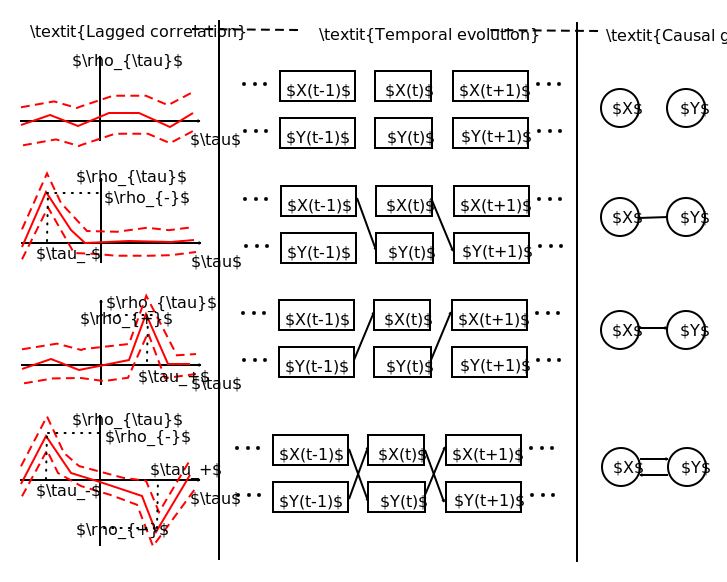
\includegraphics[width=\textwidth]{Figures/Theory/causality_twovars}
\bigskip
\framecaption{\textbf{Illustration of possible configurations in the case of two variables.}\label{frame:causalityregimes:twovars}}{\textbf{Illustration de situations possibles dans le cas de deux variables.} Pour simplifier, nous ne différencions les situations que par l'existence ou non d'un extremum pour les valeurs positives et négatives du délai $\tau$ (et ne prenons pas en compte le signe de la corrélation correspondante). Les lignes pointillées illustrent un seuil de significativité, par exemple un intervalle de confiance sur la corrélation estimée. On a donc quatre situations : aucun extremum significatif, existence de $\tau_-$, existence de $\tau_+$ et existence de $\tau_-$ et de $\tau_+$. Dans le premier, il n'y a pas de lien diachronique entre les variables (mais possiblement des corrélations simultanées, spécifiées par les doubles flèches verticales). Dans les deux suivants, l'une ``cause'' l'autre variable (nous utiliserons parfois ce raccourci sémantique pour commenter les résultats des analyses). Enfin dans la dernière, on a causalités circulaires : de tels motifs s'apparenteront à ce que l'on désignait conceptuellement par co-évolution.\label{frame:causalityregimes:twovars}}
\end{mdframed}
\end{figure}
%%%%%%%%%%%%%

%\comment{voir aussi réseau bayesiens, semble proche de l'idee de reseaux entre variables}



\subsubsection{Emergence and a proxy to measure co-evolution ?}{Emergence et mesure de la co-évolution ?}


% idee sur les repets : lors de l'agreg perd de l'information ? lie au maup..

Prenons également un court instant pour clarifier le statut épistémologique et ontologique attendu par l'application de cette méthode, et dans quelle mesure on peut espérer l'utiliser comme mesure indirecte de la co-évolution. La causalité de Granger est estimée à la fois \emph{dans le temps}, \emph{dans l'espace} et \emph{entre les répétitions}. Dans le cas où l'on observe un phénomène historique, on a une unique trajectoire et l'estimation est faite dans le temps et l'espace uniquement, mais dans tous les cas on passe de caractéristiques à l'échelle microscopique à une mesure macroscopique\footnote{Nous utilisons ici ces termes pour simplifier, il s'agit en fait d'un échelle donnée à une échelle supérieure qui dépend de l'étendue temporelle et spatiale totale.}. Ainsi, on peut avoir des interactions microscopiques circulaires, mais émergence d'un sens de la causalité au niveau macroscopique, ou l'inverse. Rejoignant la question des populations et individus pour la définition de la co-évolution en biologie (voir~\ref{sec:epistemology}), pour laquelle les adaptations mutuelles émergent au niveau des espèces, nous postulons que la caractérisation des motifs de causalité est une manière de caractériser des dynamiques co-évolutives pour les systèmes territoriaux, correspondant alors à notre définition intermédiaire de la co-évolution au niveau d'une population.


Est-il alors possible de répondre de manière équivoque à la question ``\textit{y a-t-il co-évolution dans un cas particulier}''\footnote{A laquelle nous ajoutons : pour ces composantes, sur cette portée spatiale et temporelle et sur ces échelles spatiale et temporelle.} ? Cela se saurait si nous pouvions réinventer l'eau chaude mais qui se chauffe elle-même. Nous voulons dire par là, et nous le verrons dans les multiples développements, que de nombreux problèmes fondamentaux intrinsèques à l'étude des systèmes géographiques (la question des échelles, de la définition du système, des variables prises en compte, le problème de l'observation de trajectoire uniques, de données bruitées et éparses, le problème du MAUP, etc.) seront bien toujours présents, et que la question ci-dessus qui y est naturellement soumise s'avère naïve. Mais nous verrons qu'il sera bien possible d'isoler des signaux clairs, et mettrons en évidence des cas où il existe un sens causal et d'autres où il y a circularité au niveau macroscopique.

% -> en conclusion partie II, revenir la dessus et preciser/clarifier la co-evol conceptuelle et la co-evol ``empirique'', enfin son proxy.



%%%%%%%%%%%%%%%
\subsection{Synthetic data}{Données Synthétiques}

Nous explorons et validons la méthode dans un premier temps sur données synthétiques, c'est-à-dire générées par l'intermédiaire d'un modèle avec un certain niveau de contrôle.


\subsubsection{Auto-regressive time series}{Séries temporelles auto-régressives}

Illustrons les motifs qui peuvent être attendus, notamment ceux stylisés donnés précédemment en Encadré~\ref{frame:causalityregimes:twovars}, sur des données synthétiques avec une structure simple. L'idée est de générer des séries temporelles sur lesquelles le retard et le niveau de corrélation sont contrôlés, ainsi que les résultats théoriques connus.


Soit $\vec{X}(t)$ un processus stochastique suivant l'équation d'auto-régression $\vec{X}(t) = \sum_{\tau > 0} \mathbf{A}(\tau) \cdot \vec{X}(t - \tau ) + \vec{\epsilon}(t)$. Dans le cas où $\mathbf{A}(\tau) = 0$ pour $\tau \neq \tau_0$ et $\mathbf{A}(\tau_0) = \left( {\begin{array}{cc} 0 & a \\ a & 0 \\ \end{array}} \right)$ pour $-1<a<1$, le calcul des corrélations théoriques est possible (voir Annexe~\ref{app:sec:causalityregimes}), et on obtient, en notant $\mathbf{X} = (X,Y)$, pour $\tau > 0$
\[
\rho\left[X(t),Y(t-\tau)\right] = \begin{cases}
	a^{2k+1} \textrm{si } \tau = (2k+1)\tau_0\textrm{ pour tout }k\in \mathbb{Z} \\
	0 \textrm{ sinon} 
\end{cases}
\]

L'expression est la même pour $\tau<0$ en échangeant $X$ et $Y$. Ainsi, on contrôle la corrélation retardée au retard voulu et aux retards qui en sont multiples avec un facteur impair. En changeant l'un des coefficients en 0 ou en son opposé, on obtient pour les premiers maximums les trois profils stylisés donnés en Encadré~\ref{frame:causalityregimes:twovars}.


Utilisons cet exemple pour explorer numériquement la possibilité de classifier les profils de corrélations retardées. Nous considérons le même processus pour $\tau_0 = 2$ et $\mathbf{A}(\tau_0) = \left( {\begin{array}{cc} 0 & a_1 \\ a_2 & 0 \\ \end{array}} \right)$, avec $-1<a_1,a_2<1$. Nous simulons avec ce modèle des séries temporelles de longueur $t_f=10000$ en tirant $b=10000$ valeurs aléatoires pour les paramètres $(a_1,a_2)$. Sur chaque série les corrélations retardées sont estimées, et nous procédons à une classification non-supervisée\footnote{Par algorithme des \emph{k-means} avec $k=9$ et $b_c = 1000$ répétitions.} sur les séries temporelles $\left[\rho(\tau)\right]_{a_1,a_2}$. Nous montrons en Fig.~\ref{fig:causalityregimes:arma} les profils typiques obtenus en correspondance avec leur position dans l'espace des paramètres $(a_1,a_2)$. Nous obtenons exactement les neuf profils stylisés possibles, en correspondance avec les valeurs relatives des paramètres comme attendu. À partir de profils très variés de corrélations retardées, nous sommes ainsi capable d'extraire des profils typiques d'interaction entre les variables. Cela nous renforce dans l'idée d'appliquer cette méthode sur des données plus complexes par la suite.


% comparaison correlation theorique / correlation empirique
% -> pas besoin, evident pour des ts seules. on pourrait estimer la valeur pour le centre du cluster ? pas si evident.

%%%%%%%%%%%%%
\begin{figure}
	%\includegraphics[width=0.48\linewidth]{Figures/CausalityRegimes/coefsclust_nbootstrap10000_maxai0_1_lag2nclust9.png}
	%\includegraphics[width=0.48\linewidth]{Figures/CausalityRegimes/centertrajs_nbootstrap10000_maxai0_1_lag2nclust9.png}
	\includegraphics[width=\linewidth]{Figures/Final/4-2-2-fig-causalityregimes-arma.jpg}
	\caption[Auto-regressive time-series][Séries temporelles auto-régressives]{\textbf{Estimation of correlation regimes of auto-regressive time series.}\label{fig:causalityregimes:arma}}{\textbf{Estimation des régimes de corrélation dans le cas de séries temporelles auto-régressives linéaires.} Résultats de la méthode de classification des régimes pour des processus AR simples. Nous simulons $b = 10000$ séries temporelles de longueur $t_f = 10000$, avec des coefficients aléatoires $(a_1,a_2) \in [-0.1,0.1]$ et un délai $\tau_0 = 2$. (\textit{Gauche}) Valeur des coefficients $(a_1,a_2)$, la couleur donnant le cluster obtenu ; (\textit{(Droite)}) Trajectoires de centroïdes correspondants. Nous retrouvons les profils stylisés attendus, qui correspondent aux valeurs relatives des paramètres : par exemple, le cluster 1 est pour $a_1$ faible et $a_2$ fort, et correspond bien à une situation où $\rho_+$ existe c'est-à-dire une configuration $X\rightarrow Y$, et le signe de $\rho_+$ correspond à $a_2 >0$. \label{fig:causalityregimes:arma}}
\end{figure}
%%%%%%%%%%%%%



\subsubsection{Urban growth model}{Modèle de croissance urbaine}

\bpar{
This method must first be tested and partially validated, what we propose to do on synthetic data, what allows a more refined knowledge of the behavior of models~\cite{raimbaulthalshs01514415}. Echoing the example of relations between transportation networks and territories that introduced the research question before, we generate stylized urban configurations in which network and density mutually interact, and for which causalities are not obvious \emph{a priori} knowing the parameters of the generative model.
}{
Cette méthode doit être testée et validée sur un système plus proche de nos préoccupations, ce que nous faisons à nouveau sur des données synthétiques.  En écho à l'exemple des relations entre réseaux de transport et territoires qui a permis d'introduire notre problématique précédemment, nous proposons de générer des configurations urbaines stylisées dans lesquelles réseau et densité s'influencent mutuellement, et pour lesquelles les causalités ne sont pas évidents \emph{a priori} étant donné les paramètres du modèle génératif.
}
% méthode qui permet une connaissance plus fine des comportements des modèles \cite{raimbault2016generation}.


\bpar{
\cite{raimbault2014hybrid} describes and explores a simple model of urban morphogenesis (the RBD model) that fits perfectly these constraints. Indeed, explicative variables of urban growth, processes of network extension and the coupling between urban density and the network are relatively simple. However, except for extreme cases (for example when distance to the center solely determines land value, the network will depend on density in a causal way; when only the distance to the network counts, the causality will be inverted), mixed regimes do not exhibit obvious causalities. It is for this reason an ideal case to test if the method is able to detect some.
}{
\cite{raimbault2014hybrid} décrit et explore un modèle simple de morphogenèse urbaine\footnote{Nous n'explorons pas ici le concept de morphogenèse, qui fera l'objet du chapitre~\ref{ch:morphogenesis}, mais utilisons ce modèle comme producteur de données synthétiques.} (modèle RBD) répondant à ces contraintes. Ce modèle est décrit en détails pour la configuration dans laquelle nous l'utilisons en Encadré~\ref{frame:causalityregimes:rbd}. Les variables explicatives de la croissance urbaine, les processus d'extension du réseau et le couplage entre densité urbaine et réseau ne sont pas trop complexes. Cependant, hormis dans des cas particuliers (par exemple lorsque la distance au centre détermine la valeur foncière uniquement, le réseau dépendra de manière causale de la densité, ou lorsque la distance au réseau seule compte, la causalité sera inversée), les régimes mixtes ne présentent pas de causalités évidentes : c'est donc un cas adapté pour tester si la méthode est capable d'en détecter. Les données synthétiques nous permettent de contrôler la cohérence dans les cas où la relation est attendue.
}


%%%%%%%%%%%%%
\begin{figure}[h!]
\begin{mdframed}
Le modèle RBD suppose une grille de côté $N$, dont les cellules ont un état binaire (occupée ou non). Dans la version utilisée, il existe un unique centre urbain (noeud particulier du réseau) et le réseau de transport est initialement nul. Chaque cellule $i$ est caractérisée par les variables $x_d (i)$ (densité dans un rayon fixé $r=5$), $x_r (i)$ (distance à la route la plus proche) et $x_c (i)$ (distance au centre via le réseau). Ces variables permettent de calculer une valeur de potentiel pour chaque cellule $U_i = \sum w_k \tilde{x}_k (i)$, où les $w_k$ sont des paramètres du modèle permettant d'influencer les formes urbaines produites et $\tilde{x}_k(i)$ les variables normalisées sur l'ensemble des cellules par $\tilde{x}_k(i) = \frac{\max_i x_k (i) - x_k (i)}{\max_i x_k (i) - \min_i x_k (i)}$.

Le potentiel peut être interprété comme une utilité agrégeant les préférences des agents devant se localiser. Une répulsion à la densité donnera par exemple des formes urbaines très dispersées.

Le modèle évolue séquentiellement en peuplant progressivement la grille. À chaque pas de temps :
\begin{itemize}
	\item les $N_G$ cellules avec plus grande valeur $U_i$ sont occupées de manière simultanée ;
	\item si une cellule nouvellement peuplée est à une distance au réseau supérieure à un seuil $\theta_d$ (que nous fixerons ici à $\theta_d = 5$), celle-ci est connectée au réseau par une nouvelle route prenant le chemin le plus court.
\end{itemize}

La croissance s'arrête à un temps final fixé $t_f$.

\medskip

% here example de configs
%\includegraphics[width=0.32\linewidth]{Figures/CausalityRegimes/ex_60_wdens0_wroad1_wcenter1_seed272727}
%\includegraphics[width=0.32\linewidth]{Figures/CausalityRegimes/ex_60_wdens1_wroad1_wcenter0_seed272727}
%\includegraphics[width=0.32\linewidth]{Figures/CausalityRegimes/ex_60_wdens1_wroad1_wcenter1_seed272727}
\includegraphics[width=\linewidth]{Figures/Final/4-2-2-frame-causalityregimes-rdb.jpg}
\textit{Exemples de configurations finales variées, obtenues avec les paramètres de poids $(w_{d},w_{c},w_{r})$ valant respectivement $(0,1,1)$,$(1,0,1)$, et $(1,1,1)$.}

\medskip

\framecaption{\textbf{Description of the RBD model.}\label{frame:causalityregimes:rbd}}{\textbf{Description du modèle RBD.}\label{frame:causalityregimes:rbd}}
\end{mdframed}
\end{figure}
%%%%%%%%%%%%%





\bpar{
 We use an applied implementation\footnote{available on the open repository of the project at \\\texttt{https://github.com/JusteRaimbault/CityNetwork/tree/master/Models/Simple/ModelCA}} of the original model, allowing to capture the values of studied variables for each cell of the cellular automaton and for each time step, and to calculate the lagged correlations in the sense described before, between variables of the model. We explore a grid of the parameter space of the RBD model, making the weight parameters for density, distance to center and distance toi network vary\footnote{The model works the following way: a value of cells is determined by the weighted average of these different explicative variables, value that determines the growth of new patches at the next time step.}, that we write respectively $(w_{d},w_{c},w_{r})$, in $\left[0;1\right]$ with a step of $0.1$. Other parameters are fixed to their default values given by~\cite{raimbault2014hybrid}. For each parameter value, we proceed to $N=100$ repetitions, what is enough for a good convergence of indicators. Explorations are done with the OpenMole software~\cite{reuillon2013openmole}, the large number of simulations (1,330,000) implying the use of a computation grid.
}{
Nous utilisons une implémentation adaptée\footnote{Le modèle est disponible sur le dépôt ouvert du projet à \url{https://github.com/JusteRaimbault/CityNetwork/tree/master/Models/Simple/ModelCA}.} du modèle initial, permettant de capturer les valeurs des variables étudiées pour chaque cellule et à chaque pas de temps et de calculer les correlations retardées entre variables au sein du modèle. Nous explorons une grille de l'espace des paramètres du modèle RBD, faisant varier les paramètres de poids de la densité $w_d$, de la distance au centre $w_c$ et de la distance au réseau $w_r$ (voir Encadré~\ref{frame:causalityregimes:rbd} de description du modèle), dans $\left[0;1\right]$ avec un pas de $0.1$. Les autres paramètres sont fixés à leur valeurs par défaut données par \cite{raimbault2014hybrid}. Pour chaque valeur des paramètres, nous procédons à $N=100$ répétitions ce qui est suffisant pour une bonne convergence des indicateurs. Les explorations sont effectuées via le logiciel OpenMole~\cite{reuillon2013openmole}, le grand nombre de simulations (1330000) nécessitant l'utilisation d'une grille de calcul\footnote{Les résultats de simulation sont disponibles à \url{http://dx.doi.org/10.7910/DVN/KGHZZB}.}.
}



\bpar{
We compute for all patches the lagged correlations with the unbiased Pearson estimator between the variations of the following variables\footnote{Computing the correlations directly on the variables makes no sense since their value has no absolute meaning.}: local density, distance to center and distance to network.
}{
Nous calculons sur l'ensemble des cellules les corrélations retardées par estimateur de Pearson non biaisé entre les variations des variables suivantes\footnote{Calculer les corrélations sur les variables directement n'a pas de sens puisque leur valeur n'en a pas en absolu.} : densité locale, distance au centre et distance au réseau. Il s'agit des variables explicatives pour la dynamique du modèle, et donc celles sur lesquelles on peut identifier des relations dynamiques entre caractéristiques territoriales locales.
}



%%%%%%%%%%%%%%%
\begin{figure}
\vspace{-0.5cm}
%\includegraphics[width=\linewidth]{Figures/CausalityRegimes/synth_extreme.jpg}
\includegraphics[width=\linewidth,height=0.9\textheight]{Figures/Final/4-2-2-fig-causalityregimes-exrdb.jpg}
\vspace{-0.8cm}
\caption[Correlation in the RBD model][Corrélations dans le modèle RDB]{\textbf{Correlations in the RBD model.} \textbf{(First row)} Example of different final configurations, obtained with $(w_{d},w_{c},w_{r})$ being respectively $(0,1,1)$,$(1,0,1)$, and $(1,1,1)$. \textbf{(Second row)} Lagged correlations, for each combination of parameters in $\{0,1\}$, as a function of the lag $\tau$. The different colors correspond to each couple of variables: distance to the center (\texttt{ctr}, $C$), density (\texttt{dens}, $D$) and distance to the network (\texttt{rd}, $R$). The dots show the extent on all the repetitions of the model (estimators on $i$ and $t$ only).\label{fig:causalityregimes:exrdb}}{\textbf{Correlations retardées dans le modèle RDB.} Corrélations retardées, pour chaque combinaison des valeurs extrêmes pour l'ensemble des paramètres $w_r,w_c,w_d$. Chaque graphe donne la corrélation $\rho_{\tau}$ en fonction du retard $\tau$. Les différentes couleurs correspondent à chaque couple de variables : distance au centre (\texttt{ctr}), densité (\texttt{dens}) et distance au réseau (\texttt{rd}). Les points correspondent aux corrélations individuelles pour chaque répétition du modèle (estimateurs sur $i$ et $t$), tandis que les courbes donnent l'estimateur complet sur l'ensemble des répétitions également. Pour chaque graphe, nous donnons en correspondance directe une configuration finale, et l'interprétation de terme de motifs de causalité sous forme d'un graphe entre les variables. La couleur des liens dirigés donne le signe de la relation (rouge pour corrélation négative, verte pour corrélation positive).\label{fig:causalityregimes:exrdb}}
\end{figure}
%%%%%%%%%%%%%%%



\bpar{
The figure~\ref{fig:exrdb}  shows the behavior of $\rho_{\tau}$ for each couple of variable (undirected, $\tau$ taking negative and positive values), for the combination of extreme values of parameters. We can already see different regimes emerge: for example, $(1,0,1)$ leads to a causality of density on distance to center with a lag $\tau=1$, and a negative causality of density on distance to network with the same lag, whereas distance to the center and to the network are correlated in a synchronous manner.
}{
La Fig.~\ref{fig:causalityregimes:exrdb} montre le comportement de $\rho_{\tau}$ pour chaque couple de variables (non dirigé, $\tau$ prenant des valeurs négatives et positives), pour les combinaisons des valeurs extrêmes des paramètres. Nous donnons également l'interprétation sous forme de graphe de relations entre variables et une illustration de configuration urbaine générée pour les valeurs de paramètres correspondantes.
}

\bpar{}{
Nous voyons un certain nombre de régimes émerger, et pouvons tirer les interprétations synthétiques suivantes :
\begin{itemize}
	\item Le lien négatif $D\rightarrow R$ résulte du mécanisme simple d'extension du réseau : un accroissement de la densité conduit à une diminution de la distance au réseau par la construction d'une nouvelle route. Certaines configurations inhibent ce lien, par l'interaction complexe avec les autres variables (par exemple $(0,1,0)$).
	\item Des graphes de relations élaborés peuvent émerger : $(1,0,1)$ conduit par exemple à une relation circulaire entre distance au réseau et densité, et une causalité de ces deux variables sur la distance au centre.
	\item Des comportements non attendus a priori émergent, comme par exemple la relation circulaire entre distance au réseau et distance au centre pour $(0,0,1)$ où seule la densité joue ; au contraire le modèle fait émerger une relation qui correspond au mécanisme microscopique quand $w_r=1$ seulement.
\end{itemize}
}


L'intérêt de la méthode se précise ici, puisqu'elle permet de dégager des motifs de causalité ``macroscopiques'' (c'est-à-dire effectivement mesurables à un niveau statistique), à partir de motifs ``microscopiques'' (par exemple la règle de connection de la route), et de manière non-linéaire. Des liens qu'on pourrait attendre intuitivement comme $D\rightarrow R$ sont dans certains cas inhibés. Cela confirme la pertinence de la distinction entre les deux premiers niveaux de co-évolution, la co-évolution ``processuelle'' (au niveau des entités ou des processus) et la co-évolution statistique au niveau d'une population.



\subsubsection{Causality regimes}{Régimes de causalité}

\bpar{
To study these behaviors in a systematic way, we propose to identify regimes endogenously, by using non-supervised classification. We apply a \emph{k-means} clustering, robust to stochasticity (5000 repetitions), with the following features: for each couple of variables, $\textrm{argmax}_{\tau} \rho_{\tau}$ and $\textrm{argmin}_{\tau} \rho_{\tau}$ if the corresponding value is such that $\frac{\rho_{\tau}-\bar{\rho}_{\tau}}{\left|\bar{\rho}_{\tau}\right|} > \theta$ with $\theta$ threshold parameter, 0 otherwise. The inclusion of supplementary features of values of $\rho_{\tau}$ does not significantly changes the results, these are therefore not taken into account to reduce the dimension. The choice of the number of clusters $k$ is generally a difficult problem in this kind of approach~\cite{hamerly2003learning}. In our case the system exhibit an convenient structure: the curves of inter-cluster variance proportion and its derivative in figure~\ref{fig:clustering}, as a function of $k$ for different values of $\theta$, show a transition for $\theta = 2$, what gives for the corresponding curve a break around $k=6$. A visual screening of clusters in a principal plan confirms the good quality of the classification for these values. A class corresponds then to a \emph{causality regime}, for which we can represent the phase diagram as a function of model parameters, and also cluster centers profiles (computed as the barycenter in the full initial space) in figure~\ref{fig:clustering}.
}{
Nous démontrons à présent qu'il est possible d'établir une typologie endogène des comportements des corrélations retardées. Afin d'étudier ces comportements de manière systématique, nous proposons d'identifier des régimes de manière endogène, en procédant à un apprentissage non-supervisé. Nous appliquons comme précédemment une classification des \emph{k-means}, robuste à la stochasticité (5000 répétitions), avec les points caractéristiques (\emph{features}) suivants : pour chaque couple de variable, $\textrm{argmax}_{\tau} \rho_{\tau}$ et $\textrm{argmin}_{\tau} \rho_{\tau}$ si la valeur correspondante est telle que $\frac{\rho_{\tau}-\bar{\rho}_{\tau}}{\left|\bar{\rho}_{\tau}\right|} > \theta$ avec $\theta$ paramètre de seuil, 0 sinon. L'inclusion des \emph{features} (variables caractéristiques) supplémentaires des valeurs de $\rho_{\tau}$ n'influence pas significativement les résultats, et celles-ci n'ont pas été prises en compte pour réduire la dimension. Le choix du nombre de clusters $k$ est en général épineux dans ce genre de problème~\cite{hamerly2003learning}, mais dans notre cas le système possède une structure qui lève l'ambiguïté : les courbes de la proportion de variance inter-cluster et de sa dérivée (voir  Fig.~\ref{fig:app:causalityregimes:clustering} en Annexe~\ref{app:sec:causalityregimes}), en fonction de $k$ pour différentes valeurs de $\theta$, présentent une transition pour $\theta = 2$, ce qui donne pour cette courbe une rupture à $k=5$. Un examen visuel des clusters dans un plan principal confirme la bonne qualité de la classification pour ces valeurs. Une classe correspond alors à un \emph{régime de causalité}, dont nous pouvons représenter le diagramme de phase en fonction des paramètres du modèle, ainsi que les trajectoires des centres des clusters (calculées comme barycentre dans l'espace complet initial) en Fig.~\ref{fig:causalityregimes:clustering}.
}




%%%%%%%%%%%%%%%
\begin{figure}
%\includegraphics[width=0.59\linewidth]{Figures/CausalityRegimes/clusters-paramfacet_valuesFALSEtheta2_k6}\\
%\includegraphics[width=\linewidth]{Figures/CausalityRegimes/clusters-centertrajs-facetclust_valuesFALSEtheta2_k6}]
\includegraphics[width=\linewidth]{Figures/Final/4-2-2-fig-causalityregimes-clustering.jpg}
\caption[Identification of interaction regimes][Identification de régimes d'interactions]{\textbf{Identification of regimes of interaction.} \textbf{(Top left)} Inter-cluster variance as a function of cluster number. \textbf{(Top middle)} Derivative of the inter-cluster variance. \textbf{(Top right)} Features in a principal plan (81\% of variance explained by the two first components)\textbf{(Bottom left)} Phase diagram of regimes in the space $(w_{d},w_{c},w_{r})$, $w_r$ varying between the different sub-diagrams of $(w_{d},w_{c}$. \textbf{(Bottom right)} Corresponding profiles of centroids.\label{fig:causalityregimes:clustering}}{\textbf{Régimes de causalité identifiés par classification non supervisée.} (\textit{Haut}) Diagramme de phase des régimes (cluster) dans l'espace des paramètres $(w_{d},w_{c},w_{r})$, $w_r$ variant entre les différents sous-diagrammes de $(w_{d},w_{c}$. (\textit{Bas}) Trajectoires correspondantes des centroïdes, en termes de profils de corrélations retardées $\rho_{\tau}$, pour l'ensemble des couples de variables (couleur) et pour chaque cluster.\label{fig:causalityregimes:clustering}}
\end{figure}
%%%%%%%%%%%%%%%



\subsubsection{Interpretation}{Interprétation}

\bpar{
 The behavior obtained is interesting, as regions in the diagram corresponding to the different regimes are clearly delimited and connected. For example, we observe the emergence of regime 6 in which distance to network causes strongly the density in a negative way, but distance to the center causes distance to the network. Its maximal extent on $(w_d,w_r)$ is for an intermediate value $w_r=0.7$. Thus, to maximize the impact of network on density, the corresponding weight must not be maximized, what can be counter-intuitive at first sight. It illustrates the utility of the method in the case of circular causal relations difficult to entangle a priori. The regime 5, in which distance to network influences the density the same way, but the relation between distance to center and to the network is inverted, is also interesting, and predominates for low $w_r$ values. The regime 1 is an extreme one and corresponds to an isolated situation in which distance to the center has no role: this aspect dominates then totally the other interaction processes between density and network.
}{
Nous proposons finalement d'interpréter les régimes obtenus, représentés en Fig.~\ref{fig:causalityregimes:clustering}. Le comportement obtenu est particulièrement intéressant : les régions du diagramme de phase selon les paramètres correspondant aux régimes sont clairement délimitées et connexes. Par exemple, on observe l'émergence d'un régime (numéroté 1) où la densité cause fortement la distance au réseau de manière négative (au sens de l'existence d'un $\rho_+$ négatif), mais la distance au centre cause la distance au réseau, régime dont l'étendue maximale dans le plan $(w_d,w_c)$ est pour une valeur intermédiaire $w_r=0.7$. Ainsi, pour maximiser l'impact du réseau sur la densité, il ne faut pas maximiser le poids correspondant mais prendre une valeur intermédiaire, ce qui peut paraître contre-intuitif en premier abord : cela illustre l'intérêt de la méthode dans le cas de relations circulaires difficiles à démêler a priori. Le régime 2, où la distance au réseau influence la densité de la même manière, mais la relation entre distance au centre et route est inversée, est prédominant dans les faibles $w_r$ : ainsi, l'attenuation du rôle de la distance à la route conduit le centre à inverser sa relation avec la distance à la route. Le régime 6, extrême quant à sa position dans l'espace des paramètres car dans un voisinage de $w_c = 0$, correspond à une situation isolée dans laquelle la distance au centre n'importe pas comme variable explicative, et on observe une causalité de la densité sur la distance au centre ($\rho_+$ pour $D\rightarrow R$) et de la distance à la route sur la distance au centre ($\rho_-$ pour $C\rightarrow R$), c'est-à-dire que cet aspect est totalement dominé par les autres.
}



\bpar{
This application on synthetic data demonstrate on one hand the robustness of the method given the consistence of obtained regimes, and realizes this way a much more finer qualification of model behavior than the one done in the original paper. In this precise case, it can be taken as an instrument of knowledge for relations between networks and territories in itself, allowing the test of assumption or the comparison of processes in the stylized model.
}{
Cette application sur données synthétiques démontre ainsi d'une part la robustesse de la méthode vu la cohérence des régimes obtenus, et constitue aussi une qualification beaucoup plus précise des comportements du modèle que celle réalisée dans l'article initial. Dans ce cas précis, il peut s'agir d'un instrument de connaissance des relations entre réseaux et territoires en lui-même, permettant le test d'hypothèses ou la comparaison de processus dans le modèle stylisé.
}










%--------------------------------------------------------









%%%%%%%%%%%%%%%%%%%%%%%
\subsection{Network-territory relations in South Africa}{Relations Réseaux-territoires en Afrique du Sud}



\bpar{
We assum that territorial dynamics and network dynamics responded differently to these. We expect to learn from these project informations on interactions at long time scale and large spatial scale, in a very particular context of constrained growth.
}{
Nous démontrons à présent les potentialités de notre méthode à établir des liens entre variables sur des données géo-historiques sur le temps long, pour le cas du réseau ferré en Afrique du Sud au cours du 20ème siècle. En faisant l'hypothèse que les territoires et les réseaux réagissent différemment aux événements historiques, les motifs de causalité devraient informer sur leur relations sur le temps long.
}


\subsubsection{Context}{Contexte}


\bpar{
Transportation Networks can be leveraged as a powerful socio-economic control tool, with even more significant outcomes when it percolates to their interaction with territories. The case of South Africa is an accurate illustration, as \cite{baffi:tel-01389347} shows that during apartheid railway network planning was used as a racial segregation tool by shaping strongly constrained mobility and accessibility patterns. In particular, it is shown qualitatively that dynamics between territories and networks profoundly changed at the end of the apartheid, transforming a tool of planed segregation (network shaped was optimized to minimize unwanted accessibility) into an integration tool thanks to recent changes in network topology patterns. We propose to investigate the potential \emph{structural} properties of this historical process, by focusing on dynamical patterns of interactions between the railway network and city growth. More precisely, we try to establish if the segregative planning policies did actually modify the trajectory of the coupled system, what would correspond to deeper and wider impacts. 
}{
Les réseaux de transport peuvent être utilisés comme un puissant outil de contrôle des populations, avec des effets encore plus significatifs lorsque ceux-ci perturbent les relations avec les territoires. Le cas de l'Afrique du Sud est une illustration pertinente, puisque \cite{baffi:tel-01389347} montre que lors de l'apartheid la planification du réseau ferré était utilisée comme un outil de ségrégation raciale par l'établissements de motifs de mobilité et d'accessibilité fortement contraints\footnote{La politique de ségrégation est interprétée par~\cite{baffi:tel-01389347} (p.~189) comme une intention de ``connecter sans connectivité'', conjointement avec les migrations forcées de la population ségréguée dans des zones spécifiques à l'écart des fonctions urbaines, appelées \emph{bantoustans}. Le réseau a alors été spécifiquement développé pour relier ceux-ci aux zones de production sans les connecter efficacement aux centres urbains.}. En particulier, il est montré qualitativement que les dynamiques entre réseaux et territoires ont profondément changé à la fin de l'apartheid, transformant un outil de ségrégation planifiée (une forme de réseau conçue pour minimiser l'accessibilité des populations ségréguées) en un outil d'intégration grâce à des changement récents dans la topologie du réseau. Nous étudions ici les potentielles propriétés \emph{structurelles} de ce processus historique, en se concentrant sur les motifs dynamiques des interactions entre le réseau ferré et la croissance des villes. Plus précisément, nous essayons d'établir si les politiques de planification ségrégatives ont effectivement modifié la trajectoire du système couplé, ce qui correspondrait à des impacts plus larges et profonds que leurs effets immédiats.
}



\subsubsection{Data}{Données}


\bpar{
We use a comprehensive database covering the full South African railway network from 1880 to 2000 with opening and closing dates for each station and link, together with a city database spanning from 1911 to 1991 for which consistent ontologies for urban areas have been ensured. These database are described by~\cite{baffi:tel-01389347}, but they are not open so we make available only the aggregated data we used in the analysis.
}{
Nous utilisons une base de données complète couvrant l'ensemble du réseau ferré Sud-Africain de 1880 à 2000 avec les dates d'ouverture et de fermeture pour chaque station et liaison, couplée à une base de données pour les villes s'étendant de 1911 à 1991 pour laquelle des ontologies consistantes pour les aires urbaines ont été assurées. Ces bases de données sont décrites par~\cite{baffi:tel-01389347}, mais ne sont pas ouvertes. Pour respecter notre exigence d'ouverture, nous ne mettons ainsi à disposition que les données agrégées utilisées dans l'analyse.
}



\subsubsection{Network Measures}{Mesures de réseau}

\bpar{
First, a dynamical study of network measures seem to confirm the hypothesis: a trend rupture in closeness centrality (defined for a node as the average travel time to other nodes) at a roughly constant network size evolution, at a date corresponding to the beginning of official segregative policies, suggests that the planning process after this date had in the best case no global effect on network performance, and in the worst case had intended negative effects on accessibility with the aim to physically segregate more.
}{
Une analyse préliminaire consiste à regarder l'évolution dynamique des mesures de réseau, celles-ci pouvant témoigner de ruptures dans les propriétés structurelles du réseau et donc de mutations historiques profondes. L'évolution de certaines propriétés du réseau, comme les distributions de la centralité ou de l'accessibilité, peut témoigner de l'existence d'une planification les ayant influencées. Nous montrons en Fig.~\ref{fig:causalityregimes:network} l'évolution des mesures de réseau dans le temps\footnote{Globalement, \cite{baffi:tel-01389347} (p.~154) montre que le réseau ferré sud-africain s'est développé en arborescence et que les politiques de ségrégation ont figé sa structure, l'empêchant de mailler le territoire.}, correspondant à certaines des mesures définies en~\ref{sec:staticcorrelations}. La centralité de proximité, que nous définissons comme le temps moyen de trajet vers les autres noeuds, présente un comportement intéressant. En effet, la taille du réseau et les valeurs moyennes des centralités présentent un comportement concordant, qui correspond à l'expansion initiale du réseau. Par contre, la tendance de la hiérarchie de la centralité de proximité à se réduire est soudainement rompue à la date correspondant à l'officialisation des politiques ségrégatives en 1951, alors que taille et forme géométrique globale du réseau, traduites par l'efficience, restent constants. Ainsi, dans le meilleur des cas la planification après cette date est une coincidence avec la variation de cette propriété. Il est très probable qu'elle soit en effet responsable de cette rupture de tendance, c'est-à-dire a eu les effets escomptés sur l'accessibilité, dans le but d'empêcher la diminution de la ségrégation, puisque plus la hiérarchie est faible plus le réseau est égalitaire.
}


%%%%%%%%%%%%%%
\begin{figure}[h!]
%\includegraphics[width=0.42\linewidth]{Figures/CausalityRegimes/nw_nwSize}
%\includegraphics[width=0.47\linewidth]{Figures/CausalityRegimes/nw_meanCentralities}\\
%\includegraphics[width=0.48\linewidth]{Figures/CausalityRegimes/nw_hierarchies}
%\includegraphics[width=0.41\linewidth]{Figures/CausalityRegimes/nw_efficiency}
\includegraphics[width=\linewidth]{Figures/Final/4-2-3-fig-causalityregimes-network.jpg}
\caption[Evolution of network measures][Évolution des mesures du réseau ferré sud-africain]{\label{fig:causalityregimes:network}}{\textbf{Évolution des mesures du réseau ferré sud-africain.} On calcule pour l'ensemble des dates les mesures basiques de réseau : taille, centralités résumées par leur hiérarchie et leur moyenne, efficience. Les centralités sont normalisées pour comparaison de leur variation respective ($\max \bar{bw} = 0.07$, $\max \bar{cl} = 1.5e-4$).\label{fig:causalityregimes:network}}
\end{figure}
%%%%%%%%%%%%%%



\subsubsection{Causality patterns}{Motifs de causalité}


\bpar{
We then turn to dynamical interactions between the railway network and city growth. For that, we study Granger causalities, in the large sense of correlations between lagged variables, estimated between cities growth rates and accessibility differentials due to network growth, for all cities and urban areas having a connection to the network.
We test both travel-time and population weighted accessibilities, for varying values of distance decay parameter. Lagged correlations are fitted on varying length time windows, to test for potentially varying stationarity scales.
}{
Nous examinons à présent les interactions dynamiques entre le réseau ferré et la croissance urbaine. Pour cela, nous appliquons la méthode développée dans la première partie, qui consiste à l'étude des causalités de Granger, au sens large des corrélations entre les variables retardées, estimées entre les différentiels de population des villes et les différentiels d'accessibilité dus à la croissance du réseau, pour toutes les villes ou aires urbaines ayant une connection au réseau. Nous testons à la fois l'accessibilité en termes de distance et pondérée par la population à l'origine et aux deux extrémités. Si $P_i$ sont les populations, $d_{ij}$ la matrice de distance dans le réseau, l'accessibilité de $i$ sera donnée par $Z_i = w_i \sum_j w_j \exp \left(- d_{ij} / d_0 \right)$ où $d_0$ est le paramètre de décroissance et les poids $w_i$ sont $1/N$ ou $P_i / \sum_j P_j$ selon la modalité. Nous faisons varier les valeurs de $d_0$ pour prendre en compte les relations à différentes échelles spatiales. De plus les corrélations retardées sont estimées sur des fenêtres temporelles de taille variable $T_W$, pour tester différentes échelles potentielles de stationnarité temporelle.
}

% rq : should test log returns of variables ?

\bpar{
Results are shown in Figure~\ref{fig:causalityregimes:sudafcorrs}. We find that results are significant with travel-time accessibility only, autocorrelation dominating with weighted accessibility. A time-window of 30 years appears to be a good compromise between the number of significant correlations ($p<0.1$ for a Fisher test) and the absolute correlation level across all lags and distance decays, what should correspond roughly to the time-stationarity scale of the system. We observe furthermore a phase transition when distance decay increases, revealing the shift between the spatial scale of urban areas and the scale of the country, what gives local spatial stationarity scale.
}{
Les résultats des estimations sont montrés en Figure~\ref{fig:causalityregimes:sudafcorrs}. Nous obtenons des résultats significatifs avec l'accessibilité non-pondérée seulement, que nous montrons ici\footnote{Nous donnons en Annexe~\ref{app:sec:causalityregimes}, Fig.~\ref{fig:app:causalityregimes:sudafcorrs} les profils de corrélations retardées estimées pour les accessibilités pondérées à l'origine et à l'origine et à la destination. L'auto-corrélation domine a priori l'accessibilité pondérée : en effet, on a pour les deux variables pondérées des valeurs positives pour les faibles valeurs de $d_0$ uniquement, les autres n'étant pas significatives.}. Le meilleur compromis pour la fenêtre temporelle apparaît être une trentaine d'année, si on cherche à avoir à la fois un bon nombre de corrélations significatives (définies par $p<0.1$ pour un test de Fisher) et un niveau moyen élevé de corrélation absolue sur l'ensemble des retards et des paramètres de décroissance. Nous interprétons cette valeur comme approximativement l'échelle spatiale de stationnarité du système. Il s'agirait de la durée sur laquelle un régime du système urbain est relativement stable, et est du même ordre de grandeur que la durée de l'apartheid. 

 De plus, le nombre de corrélations significatives présente clairement une transition de phase dans ses valeurs intermédiaires en fonction de $d_0$ (Fig.~\ref{fig:app:causalityregimes:sudafcorrs}), ce qui devrait correspondre au passage entre l'échelle spatiale des aires urbaines et celle du pays, et donne ainsi l'échelle locale de stationnarité spatiale, autour de $d_0 = 500km$. Les villes du Cap et de Johannesburg sont à 1400km de distance et correspondent à deux régions aux extrémités du pays : cette échelle est donc une échelle régionale, inférieure à celle du système urbain du pays.
}


\bpar{
We obtain therethrough clear causality patterns, namely an inversion of the Granger causality (lagged correlation up to 0.5 for several values of distance decay), from accessibility causing population growth with a lag of 10-20 years before the apartheid (1948), to the opposite after the apartheid (lag 20 years). We interpret these as \emph{Structural segregation}, i.e. a significant impact of planning policies on dynamics of interactions between networks and territories. Indeed, the first regime corresponds to direct effect of transportation on migrations in a free context in opposition to the second one.
}{
L'examen du comportement des corrélations retardées en Fig.~\ref{fig:causalityregimes:sudafcorrs} conduit à l'observation de motifs de causalité assez clairs, puisque le sens de la causalité de Granger s'inverse autour de 1950, celle-ci étant à chaque fois marquée par des corrélations allant jusqu'à 0.5 pour certaines valeurs du paramètre de décroissance. On passe ainsi d'une accessibilité causant la croissance de la population avec un délai de 10 à 20 ans avant l'apartheid (1948), à l'opposé, c'est-à-dire une population induisant les changements d'accessibilité après l'apartheid (avec un délai de 20 ans).

Ce résultat est en cohérence avec les relocalisations de population et la conception du réseau en accord avec celles-ci. Nous interprétons ce phénomène comme une \emph{ségrégation structurelle}, c'est-à-dire un impact significatif des politiques de planification sur les dynamiques des interactions entre les réseaux et les territoires. En effet le premier régime peut être interprété comme un effet direct du transport sur les motifs de migration dans un contexte de liberté, en opposition au second régime qui correspondrait à un contrôle de la population et d'une adaptation du réseau en fonction. Ainsi, l'évènement historique a eu un effet au second ordre sur les relations dynamiques. Ces motifs rejoignent les conclusions empiriques obtenues par~\cite{baffi:tel-01389347} sur le sujet de l'apartheid, qui montre par exemple un fort effet des mesures sur les déplacements forcés de population, ainsi qu'une baisse de l'accessibilité pour les zones cibles de la ségrégation. 

}


% annees et duree moyenne des periodes
%
% years = c(1911,1921,1936,1951,1960,1970,1980,1991)
% #mean(years[3:length(years)] - years[1:(length(years)-2)])
% #23.16667

% effectifs
% length(unique(popdiff$id))
% [1] 798


%%%%%%%%%%%%%%
\begin{figure}
%\includegraphics[width=\linewidth]{Figures/CausalityRegimes/laggedCorrs_time_Tw3.png}
\includegraphics[width=\linewidth]{Figures/Final/4-2-3-fig-causalityregimes-sudafcorrs.jpg}
\caption[Lagged correlations in South Africa][Corrélations retardées entre croissance de population et gain d'accessibilité en Afrique du Sud]{\label{fig:causalityregimes:sudafcorrs}}{\textbf{Corrélations retardées.}  Corrélations retardées en fonction du délai $\tau$, pour la fenêtre temporelle $T_W=3$, sur les différentes périodes successives (colonnes), et pour $d_0$ variable (couleur). Pour interpréter, on observe un maximum de la corrélation retardée qui se décale dans le temps passant d'un retard négatif à un retard positif, ce qui selon notre définition correspond à une inversion du sens de la causalité.\label{fig:causalityregimes:sudafcorrs}}
\end{figure}
%%%%%%%%%%%%%%



\subsubsection{Possible developments}{Développements possibles}

\bpar{
Further work should consist in similar study with more precise socio-economic variables, for example quantifying directly segregation patterns. The method of instruments in statistics~\cite{angrist1996identification} is used to identify causal relationships between variables, in a different way than Granger causality test for example. Trying to identify causalities between network dynamics and territorial dynamics is of crucial importance to test our theoretical assumption on the existence of co-evolution.
}{
Une première extension pourra consister en une étude similaire avec des variables socio-économiques plus précises, pour quantifier par exemple directement les motifs de ségrégation. D'autre part, des variables qualitatives liées aux évènements historiques pourraient faire office de variable d'instrumentation. La méthode des variables instrumentales~\cite{angrist1996identification} est utilisée pour identifier des relations causales entre variables, d'une façon complémentaire à celle que nous avons mis en place. Nous pourrions chercher à rendre nos conclusions plus robustes, notamment vérifier si les corrélations ne sont pas fortuites, par l'application de cette approche, qui serait cependant difficile à réaliser vu la rareté des données dans notre cas.
}





\stars


% transition


Nous avons jusqu'ici dans ce chapitre exploré deux ingrédients de la théorie évolutive des villes, qui nous seront cruciaux pour comprendre la co-évolution entre réseaux de transport et territoires, à savoir les propriétés de non-stationnarité des corrélations, qui guideront la mise en place des modèles à une échelle similaire (chapitre~\ref{ch:morphogenesis} puis chapitre~\ref{ch:mesocoevolution}) et la possibilité de mise en évidence de régimes de causalité, qui nous servira d'outil de caractérisation de la co-évolution.

Nous proposons à présent d'introduire un dernier élément crucial de la théorie évolutive des villes, qui est l'appréhension des systèmes urbains par l'intermédiaire de modèles d'interaction entre villes. Ceux-ci ne seront pas co-évolutifs dans un premier temps mais leur ontologie visera à intégrer le rôle des réseaux dans le système urbain.



\stars






%
% 4.3 - Interaction Gibrat




\todo{insert / translate Interaction-Gibrat paper}





%
% Conclusion




%----------------------------------------------------------------------------------------

\newpage


\section*{Chapter Conclusion}{Conclusion du Chapitre}


La notion de co-évolution, qui était jusqu'ici relativement conceptuelle, apparaît sous de multiples angles nouveaux complémentaires. Ce chapitre permet d'éclairer son rôle au sein de la Théorie Evolutive.%\comment[FL]{cette facon de commencer et terminer les chapitres ressemble a une publicite pour la theorie evolutive. il faut exercer sont esprit critique.}
 Celle-ci sera également centrale pour la construction théorique que nous élaborerons en~\ref{sec:theory}. En effet, des interdépendances fortes peuvent se traduire par des corrélations locales variables, c'est à dire une non-stationnarité spatiale, induite d'une part par les motifs locaux correspondant à une régime d'interaction donné, dont nous avons pu capturer les manifestations statiques en section~\ref{sec:staticcorrelations}, d'autre part par le caractère multi-scalaire des processus impliqués que nous avons également montré, et donc par les interactions à grande échelle et portée entre les différentes entités territoriales, que nous avons illustré sur un cas simple par le modèle d'interaction étudié en~\ref{sec:interactiongibrat}, qui a déjà pu permettre de révéler indirectement des effets de réseaux dans les systèmes de villes. On a également éclairé une approche dynamique de la co-évolution, en montrant la complexité potentielle de la structure des relations causales dans le cas d'un modèle de morphogenèse urbaine simple. La méthodologie développée s'est montrée également efficace sur les données réelles de l'Afrique du Sud sur le temps long, permettant de découvrir un effet des politiques de ségrégation au second ordre sur la co-évolution elle-même. La question de la non-stationnarité et de la non-ergodicité dans les systèmes urbains est cruciale mais très peu comprise, et nous l'avons à peine effleurée. Dans notre cas, l'aspect le plus important de celle-ci pour la construction des modèles est son implication pour les échelles considérées, et les hypothèses d'équilibre ou de stochasticité correspondantes. On y reviendra par un point de vue différent en Chapitre~\ref{ch:morphogenesis}.
 % Nous proposons pour l'instant de renforcer l'épaisseur thématique des relations considérées : on a en effet pour l'instant seulement étudié des variables très simples (distribution de la population et propriétés du réseau) à certaines échelles seulement. On étudiera ainsi dans le prochain Chapitre~\ref{ch:micro} des ontologies et échelles sur des cas d'étude plus exotiques.



\stars


%%%%%%%%%%%%%%%



%%%%%%%%%%%%%%%
% Chapter 5 : Micro-level Interactions




% Chapter 

\chapter{Interactions at the Micro Level}{Interactions au niveau microscopique} % Chapter title

\label{ch:micro} % For referencing the chapter elsewhere, use \autoref{ch:name} 

%----------------------------------------------------------------------------------------


\headercit{}{}{}


\bigskip













%----------------------------------------------------------------------------------------


% section : heterogenous bike-sharing
% a priori will not do this -

%\section{Shared Transportation System}{Système de Transport en Partage}










%
% 5.1 - Transportation Equilibrium


%\newpage

%----------------------------------------------------------------------------------------


%\section[Static User Equilibrium][Equilibre Utilisateur Statique]{Investigating the Empirical Existence of Static User Equilibrium}{Investigation Empirique de l'Existence de l'Equilibre Utilisateur Statique}

%\section{Static User Equilibrium}{Dynamique des flux de trafic routier}

%\subsubsection{Illustration of the construction and the use of an open dataset}{Illustration de la construction et de l'utilisation d'un jeu de données ouvertes}

%\label{sec:transportationequilibrium}



%----------------------------------------------------------------------------------------


%\bpar{
%The Static User Equilibrium is a powerful framework for the theoretical study of traffic. Despite the restricting assumption of stationary flows that intuitively limit its application to real traffic systems, many operational models implementing it are still used without an empirical validation of the existence of the equilibrium. We investigate its existence on a traffic dataset of three months for the region of Paris, FR. The implementation of an application for interactive spatio-temporal data exploration allows to hypothesize a high spatial and temporal heterogeneity, and to guide further quantitative work. The assumption of locally stationary flows is invalidated in a first approximation by empirical results, as shown by a strong spatial and temporal variability in shortest paths and in network topological measures such as betweenness centrality. Furthermore, the behavior of spatial autocorrelation index of congestion patterns at different spatial ranges suggest a chaotic evolution at the local scale, especially during peak hours. We finally discuss the implications of these empirical findings and describe further possible developments based on the estimation of Lyapunov dynamical stability of traffic flows.
%}{
%L'Equilibre Utilisateur Statique est un cadre puissant pour l'étude théorique du trafic. Malgré l'hypothèse de stationnarité des flots qui intuitivement limite son application aux systèmes de trafic réels, de nombreux modèles opérationnels qui l'implémentent sont toujours utilisés sans validation empirique de l'existence de l'équilibre. Nous étudions celle-ci sur un jeu de données de trafic couvrant trois mois sur la région parisienne. L'implémentation d'une application d'exploration interactive de données spatio-temporelles permet de formuler l'hypothèse d'une forte hétérogénéité spatiale et temporelle, guidant les études quantitatives. L'hypothèse de flux localement stationnaires est invalidée en première approximation par les résultats empiriques, comme le montrent une forte variabilité spatio-temporelle des plus courts chemins et des mesures topologiques du réseau comme la centralité de chemin. De plus, le comportement de l'index d'autocorrelation spatiale pour les motifs de congestion à différentes portées spatiales suggère une évolution chaotique à l'échelle locale, en particulier lors des heures de pointe. Nous discutons finalement les implications de ces résultats empiriques et proposons des possibles développements futurs basés sur l'estimation de la stabilité dynamique au sens de Lyapounov des flots de trafic.
%}





%La mise en évidence d'une co-évolution comme nous l'avons définie, entre par exemple les motifs de congestion et ceux de localisation des actifs et des emplois, nécessiterait une source de données précise à l'échelle microscopique sur les deux aspects, et s'étendant sur une durée temporelle permettant de couvrir une part significative de relocalisations (au moins une dizaine d'années). N'ayant pas accès à de telles données, nous proposons un compromis en se basant uniquement sur des données de trafic microscopique.
%L'objectif de cette section est ainsi d'étudier indirectement les interactions entre réseaux de transport et territoires, par l'intermédiaire de la dynamique de flux de trafic routier. Ceux-ci sont en effet conditionnés par la distribution des activités sur le territoires, mais aussi par la forme du réseau. Il relèvent ainsi de l'usage du réseau, et seraient une matérialisation des interactions. Nous proposons ici de mettre à l'épreuve cette hypothèse en étudiant leur propriétés dynamiques. Plus particulièrement, nous nous intéresserons aux propriétés de non-stationnarité dans le temps et l'espace (dans l'esprit de~\ref{sec:staticcorrelations}), celles-ci étant liées au concept d'équilibre utilisé en étude du trafic comme nous allons le développer.


% \cite{barthelemy2016global}

%%%%%%%%%%%%%%%%%%%%%%%
%\subsection{Context}{Contexte}



%%%%%%%%%%%%%%%%%%%%%
%\subsection{Results}{Résultats}


%%%%%%%%%%%%%%%%%%%%%
%\subsubsection{Data collection}{Collecte des données}



%%%%%%%%%%%%%%%%%%%%%%
%\subsubsection{Methods and Results}{Méthodes and Résultats}



%%%%%%%%%%%%%%%%%%%%
%\subsection{Discussion}{Discussion}

%\subsubsection{Theoretical and practical implications of empirical conclusions}{Implications théoriques et pratiques des conclusions empiriques}

%\bpar{
%We argue that the theoretical implications of our empirical findings do not imply in a total discarding of the Static User Equilibrium framework, but unveil more a need of stronger connections between theoretical literature and empirical studies. If each newly introduced theoretical framework is generally tested on one on more case study, there are no systematic comparisons of each on large and different datasets and on various objectives (prediction of traffic, reproduction of stylized facts, etc.) as systematic reviews are the rule in therapeutic evaluation for example. This imply however broader data and model sharing practices than the current ones. The precise knowledge of application potentialities for a given framework may induce unexpected developments such as its integration into larger models.
%}{
%Nous formulons l'interprétation que les implications théoriques de ces résultats empiriques n'impliquent pas nécessairement un rejet total du cadre de l'Equilibre Utilisateur Statique, mais révèlent plutôt un besoin de plus fortes connexions entre la littérature théorique et les études empiriques. Si chaque nouveau cadre théorique introduit est généralement testé sur un cas ou plus, il n'existe pas de comparaisons systématiques de chacun sur des jeux de données de grande taille et variés, et pour des objectifs d'application différents (prédiction du traffic, reproduction de faits stylisés, etc.), à l'image des revues systématiques qui sont la règle en évaluation thérapeutique par exemple~\cite{bastian2010seventy}. Cela implique cependant des pratiques de partage des données et des modèles plus larges que celles existant couramment. La connaissance précise des potentialités d'application d'un cadre donné peut induire des développements inattendus comme l'intégration dans des modèles plus larges.
%}

%\bpar{
%The example of Land-use and Transportation Interaction studies (LUTI models) is a good illustration of how the SUE can still be used for larger purpose than transportation modeling. \cite{kryvobokov2013comparison} describe two LUTI models, one of which includes two equilibria for four-step transportation model and for land-use evolution (households and firms relocation), the other being more dynamical. The conclusion is that each model has its own advantages regarding the pursued objective, and that the static model can be used for long time policy purposes, whereas the dynamic model provide more precise information at smaller time scale. In the first case, a more complicated transportation module would have been complicated to include, what is an advantage of the static user equilibrium.

%}{
%L'exemple des études des interaction entre Transport et Usage du Sol (modèles \emph{LUTI}) est une bonne illustration d'un cas ou le EUS peut toujours être utilisé avec des motivations plus larges que la modélisation du trafic. \cite{kryvobokov2013comparison} décrit deux modèles \emph{LUTI}, dont l'un inclut deux équilibres pour les modèles de transport à quatre temps et pour l'évolution de l'usage du sol (localisation des ménages et emplois), l'autre étant dynamique. La conclusion est que chaque modèle à ses avantages au regard de l'objectif poursuivi, et que le modèle statique peut être utilisé pour comparer des politiques sur le temps long, puisque l'agrégation est moins biaisée sur le temps long. Au contraire, le modèle dynamique fournit de l'information plus précise à de plus petites échelles temporelles. Dans le premier cas, un module de transport plus compliqué aurait été plus difficile à inclure, ce qui est un avantage du EUS dans ce cas.
%}


%\bpar{
%Concerning practical applications, it seems natural that static models should not be used for traffic forecast and management at small time scales (week or day) and efforts should be made to implement more realistic models. However the use of models by the planning and engineering community is not necessarily directly related to academic concerns and state-of-the-art. For the particular case of France and mobility models, \cite{commenges:tel-00923682} showed that engineers had gone to the point of constructing inexistent problems and implementing corresponding models that they had imported from a totally different geographical context (planning in the United States). The use of one framework or type of model has historical reasons that may be difficult to overcome.
%}{
%Concernant les applications pratiques, nous suggérons que les modèles statiques ne devraient pas être utilisés pour la prédiction du trafic sur de petites échelles temporelles (semaine ou jour)\footnote{Sachant que des applications sur des échelles plus longues dans une logique de flux moyen, souvent en couplage avec des modèles LUTI, est plus raisonnable.} puisque leur hypothèse centrale n'est pas vérifiée, et que des efforts doivent être faits pour implémenter des modèles plus réalistes. Cependant, l'utilisation des modèles par la communautés des ingénieurs et des planificateurs n'est pas directement reliée aux enjeux académiques et à l'état de l'art dans le domaine. Dans le cas particulier de la France et des modèles de mobilité, \cite{commenges:tel-00923682} a montré que les ingénieurs allaient jusqu'au point de construire des problèmes inexistants et d'implémenter les modèles correspondants qu'ils avaient importé d'un contexte géographique totalement différent (la planification aux Etats-Unis). L'utilisation d'un cadre ou d'un type de modèle a des raisons historiques qui peuvent être difficiles à surmonter.
%}


%\subsubsection{Towards explanative interpretations of non-stationarity}{Sources de non-stationnarité}


%\bpar{
%An assumption we formulate regarding the origin of non-stationarity of network flows, in view of data exploration and quantitative analysis of the database, is that the network is at least half of the time highly congested and in a critical state. The off-peak hours are the larger potential time windows of spatial and temporal stationarity, but consist in less than half of the time. As already interpreted through the behavior of autocorrelation indicator, a chaotic behavior may be at the origin of such variability in the congested hours. The same way a supercritical fluid may condense under the smallest external perturbation, the state of the link may qualitatively change with a small incident, producing a network disruption that may propagate and even amplify. The direct effect of traffic events (notified incidents or accidents) can not be studied without external data, and it could be interesting to enrich the database in that direction. It would allow establishing the proportion of disruptions that do appear to have a direct effect and quantify a level of criticality of network congestion in time, or to investigate more precise effects such as the consequences of an incident on traffic of the opposite lane.
%}{
%Une hypothèse qu'on peut formuler concernant l'origine de la non-stationnarité des flots dans le réseau, au regard de l'exploration des données et des analyses quantitatives, est que le réseau est au moins la moitié du temps fortement congestionné et dans un état critique. Les heures creuses sont les plus grandes fenêtres temporelles potentielles de stationnarité spatiale et temporelle, mais couvre moins de la moitié du temps. Comme déjà interprété dans le comportement de l'indicateur d'auto-corrélation, un comportement chaotique pourrait être à l'origine d'une telle variabilité lors des heures congestionnées. A la manière d'un fluide supercritique qui condense sous une perturbation externe infinitésimale, l'état d'un lien peut qualitativement changer par un petit incident, produisant une perturbation du réseau qui se propage et peut même s'amplifier.

%L'effet direct des évènements du trafic (incidents signalés ou accidents) peut difficilement être étudié sans source de données extérieure, et un enrichissement de la base de données dans cette direction pourrait être intéressante. Cela permettrait d'établir la proportion de perturbations qui paraissent avoir un effet direct et quantifier un niveau de caractère critique de la congestion du réseau dans le temps, ou d'étudier plus précisément des phénomènes localisés comme les conséquences d'un incident de trafic sur la voie opposée.
%}



%\subsubsection{Possible developments}{Développements}


%\bpar{
%Further work may be planned towards a more refined assessment of temporal stability on a region of the network, i.e. the quantitative investigation of consideration of peak stationarity given above. To do so we propose to compute numerically Liapounov stability of the dynamical system ruling traffic flows using numerical algorithms such as described by~\cite{goldhirsch1987stability}. The value of Liapounov exponents provides the time scale by which the unstable system runs out of equilibrium. Its comparison with peak duration and average travel time, across different spatial regions and scales should provide more information on the possible validity of the local stationarity assumption. This technique has already been introduced at an other scale in transportation studies, as e.g.~\cite{tordeux2016jam} that study the stability of speed regulation models at the microscopic scale to avoid traffic jams.
%}{
%Des extensions possibles de ce travail pourront être planifiées dans la direction d'une étude de la stabilité temporelle sur des zones du réseau, i.e. l'étude quantitative précise de la non-stationnarité des heures de pointes mise en valeur ci-dessus. Pour cela nous proposons de calculer numériquement la stabilité de Liapounov du système dynamique régissant les flots de traffic, par l'intermédiaire d'algorithmes numériques comme ceux décrits par~\cite{goldhirsch1987stability}. La valeur des exposants de Liapounov fournit la vitesse typique avec laquelle le système instable s'éloigne de l'équilibre. Leur comparaison avec la durée des heures de pointe et le temps de trajet moyen, sur différentes zones spatiales et différentes échelles, devrait fournir plus d'information sur une possible validité de l'hypothèse de stationnarité locale. Cette technique a déjà été introduite à une autre échelle dans les études de transport, comme e.g.~\cite{tordeux2016jam} qui étudie la stabilité des modèles de régulation de vitesse à l'échelle microscopique pour éviter l'émergence de congestion.
%}


%\bpar{
%Other research directions may consist in the test of other assumptions of static user equilibrium (as the rational shortest path choice, which would be however difficult to test on such an aggregated dataset, implying the use of simulation models calibrated and cross-validated on the dataset to compare assumptions, without necessarily a direct clear validation or invalidation of the assumption), or the empirical computation of parameters in stochastic or dynamical user equilibrium frameworks. 
%}{
%D'autres directions de recherche peuvent consister en le test des autres hypothèses du EUS (comme le choix rationnel du plus court chemin, qui serait cependant difficile à tester à un tel niveau d'agrégation, impliquant l'utilisation de modèles de simulation calibrés par validation croisée sur le jeu de données pour comparer différentes hypothèses, sans toutefois nécessairement une validation ou invalidation directe de l'hypothèse), ou le calcul empirique des paramètres dans les cadres d'Equilibre Utilisateur Stochastique ou Dynamique.
%}



%\subsubsection{Conclusion}{Conclusion}




%\stars

%Nous avons ainsi dans cette section apporté un éclairage nouveau par rapport à notre travail principal sur les interactions entre réseaux de transport et territoires, du point de vue d'une étude empirique du trafic routier à l'échelle microscopique.

%Nous proposons dans la section suivante un développement similaire, mais à l'échelle mesoscopique et en prenant en compte un aspect économique crucial des réseaux de transport, à savoir la distribution spatiale du prix de l'énergie.

%\stars





%
% 5.2 - Energy Price


\newpage

%----------------------------------------------------------------------------------------

\section{Road Network and Prices Drivers}{Transport routier et déterminants des Coûts}

\label{sec:energyprice}

Les interactions entre réseaux et territoires peuvent se manifester indirectement au sein de propriétés économiques locales de territoires : ainsi, le prix de l'énergie conditionne fortement l'impédance d'un réseau routier, et donc son impact sur les territoires, et réciproquement ce prix est localement produit par des sous-marchés qui sont partie intégrante des territoires. La géographie des prix du carburant est donc un marqueur indirect des interactions. Par exemple, \cite{orfeuil2012grand} (p.~307) suggère un lien entre prix de l'essence et crise immobilière en région parisienne.


\stars

\textit{Cette annexe a été réalisée en collaboration avec l'économiste \noun{Dr. A. Bergeaud} (Banque de France), dans le cadre d'une convergence des problématiques entre marchés de l'énergie et observation indirecte des interactions entre réseaux et territoires. Elle a été présenté à la conférence EWGT 2017 comme \cite{raimbault2017cost}.}



\stars



\bpar{
The geography of fuel prices has many various implications, from its significant impact on accessibility to being an indicator of territorial equity and transportation policy. In this paper, we study the spatio-temporal patterns of fuel price in the US at a very high resolution using a newly constructed dataset collecting daily oil prices for two months, on a significant proportion of US gas facilities. These data have been collected using a specifically-designed large scale data crawling technology that we describe.
}{
La géographie des prix du carburant a de nombreuses applications variées, de son impact significatif sur l'accessibilité à son rôle comme indicateur d'équité territoriale et de politique de transports. Dans cette section, nous étudions les variations spatio-temporelles des prix du carburant aux États-Unis à une résolution très fine, par l'utilisation d'un nouveau jeu de données, donnant les prix journaliers sur deux mois pour une proportion significative des stations essence (autour de 70\% des stations existantes). Les données ont été collectées par l'intermédiaire d'une technologie de crawling à grande échelle élaborée spécifiquement, que l'on décrira.
}

\bpar{
We study the influence of socio-economic variables, by using complementary methods: Geographically Weighted Regression to take into account spatial non-stationarity, and linear econometric modeling to condition at the state and test county level characteristics. The former yields an optimal spatial range roughly corresponding to stationarity scale, and significant influence of variables such as median income or wage per job, with a non-simple spatial behavior that confirms the importance of geographical particularities. On the other hand, multi-level modeling reveals a strong state fixed effect, while county specific characteristics still have significant impact. Through the combination of such methods, we unveil the superposition of a governance process with a local socio-economical spatial process. We discuss one important application that is the elaboration of locally parametrized car-regulation policies.
}{
Nous étudions l'influence de variables socio-économiques, en utilisant des méthodes complémentaires : la Régression Géographique Pondérée pour tenir compte de la non-stationnarité spatiale, et une modélisation économétrique linéaire pour conditionner à l'État et tester des caractéristiques au niveau du comté. La première fournit une portée spatiale endogène qui correspond globalement à l'échelle de stationnarité, et une influence significative des variables comme le revenu moyen ou le salaire par travail, avec un comportement spatial dont la non simplicité confirme l'importance des particularités géographiques. D'autre part, la modélisation multi-niveaux révèle un très fort effet État, alors que les caractéristiques spécifiques au comté gardent un impact significatif. A travers la combinaison de ces méthodes, nous démontrons la superposition d'un processus de gouvernance avec un processus spatial socio-économique local. Nous discutons une application potentielle importante qui est l'élaboration de politiques de régulation automobiles localement paramétrisées.
}




%%%%%%%%%%%%%%%%%%%%%%
\subsection{Context}{Contexte}
\label{main}


\bpar{
What drives the price of fuel? Using a new database on oil price at a gas station level collected during two months, we explore its variability across time and space. Variation in the cost of fuel can have many causes, from the crude oil price to local tax policy and geographical features, all having heterogeneous effect in space and time. If the evolution of the average fuel price in time is an indicator that is carefully followed and analyzed by many financial institution, its variability across space remain a rather unexplored topic in the literature. Yet, such differences can reflect variation in more indirect socio-economic indicators such as territorial inequalities and geographical singularities or consumer preferences.
}{
Quels sont les déterminants des prix du carburant ? Par l'utilisation d'une nouvelle base de données des prix du carburant au niveau de la station essence, collectée pendant deux mois, nous explorons leur variabilité dans le temps et l'espace. Une variation du coût du carburant peut avoir de nombreuses causes, du prix brut du pétrole au politiques fiscales locales et aux caractéristiques géographiques, chacun ayant des effets hétérogènes dans l'espace et le temps. Bien que l'évolution du prix moyen du carburant dans le temps soit un indicateur suivi avec attention et analysé par de nombreuses institutions financières, sa variabilité dans l'espace reste relativement non-explorée dans la littérature. Cependant, de telles différences peuvent refléter des variations dans des indicateurs socio-économiques plus indirects comme des inégalités territoriales, des singularités géographiques ou des préférences des consommateurs.
}


\bpar{
There exists to our knowledge no systematic mapping in space and time of retail fuel prices for a country. The main reason is probably that the availability of data have been a significant obstacle. It is also likely that the nature of the problem may also have influence, as it lies at the crossroad of several disciplines. While economists study price elasticity and measurement in different markets, transportation geography with method such as transportation prices in spatial models, puts more emphasis on spatial distribution than on precise market mechanisms. Nevertheless, examples of somehow related works can be found. For example,~\cite{rietveld2001spatial} studies the impact of cross-border differences in fuel price and the implications for gradual spatial taxation in  Netherlands. At the country-level, \cite{rietveld2005fuel} provides statistical models to explain fuel price variability across European countries. \cite{macharis2010decision} models the impact of spatial fuel price variation on patterns of inter-modality, implying that the spatial heterogeneity of fuel prices has a strong impact on user behavior. With a similar view on the geography of transportation, \cite{gregg2009temporal} studies spatial distribution of gas emission at the US-state level. The geography of fuel prices also have important implications on effective costs, as shows \cite{combes2005transport} by determining accurate transportation costs across urban areas for France. More closely related to our work, and using very similar daily open data for France, \cite{gautier2015dynamics} investigate dynamics of transmission from crude oil prices to fuel retail prices. However, they do not introduce an explicit spatial model of prices diffusion and do not study spatio-temporal dynamics.
}{
Il n'existe à notre connaissance pas de cartographie systématique dans le temps et l'espace des prix de vente à l'échelle d'un pays à une résolution fine\footnote{En France, les données au niveau de la station sont mises à disposition en données ouvertes, à \url{https://www.prix-carburants.gouv.fr}. Le site ne permet toutefois pas de cartographie interactive dans le temps et l'espace.}. La raison principale est probablement que la disponibilité des données a pu être un obstacle important. Il est aussi probable que la nature de la question joue un rôle, puisque celle-ci se trouve à l'interface de plusieurs disciplines. Alors que les économistes étudient l'élasticité des prix et leur mesure dans différents marchés, la géographie et la socio-économie des transports, par des méthodes comme les prix des transports intégrés aux modèles spatiaux, met une emphase plus grande sur la distribution spatiale que sur des mécanismes précis de marché. 

Toutefois, des exemples de travaux relativement liés peuvent être trouvés. Par exemple, \cite{rietveld2001spatial} étudient l'impact de différences de prix transfrontalières et leur implications pour une taxation spatiale graduelle aux Pays-Bas. À l'échelle du pays, \cite{rietveld2005fuel} fournit des modèles statistiques pour expliquer les variabilité des prix entre les pays Européens. \cite{macharis2010decision} modélise l'impact d'une variation spatiale des prix sur les motifs d'intermodalité, en faisant l'hypothèse que l'hétérogénéité spatiale des prix du carburant a un impact sur le comportement des utilisateurs. Avec une approche similaire par la géographie des transports, \cite{gregg2009temporal} étudie la distribution spatiale des émissions à l'échelle des États américains.

La géographie des prix du carburant a également d'importantes répercussions sur les coûts effectifs de transport, comme le montrent \cite{combes2005transport} en déterminant les coûts réels de transport pour les différentes aires urbaines françaises. De façon plus proche de notre travail, et en utilisant des données similaires en Accès Ouvert pour la France, \cite{gautier2015dynamics} étudient les dynamiques de transmission des prix bruts du pétrole aux prix de vente. Toutefois, ils n'introduisent pas de modèle spatial explicite de diffusion des prix et n'étudient pas de dynamiques spatio-temporelles.
}


\bpar{
In this paper we adopt a different approach by proceeding to exploratory spatial analysis on US fuel prices. We show that most of the variation occurs between counties and not across time, although crude oil price was not constant during the period considered. We therefore turn to a spatial analysis of the distribution of fuel prices. Our main findings are twofold: first we show that there are significant spatial pattern in some large US regions, second we show that even if most of the observed variation can be explained by state level policies, and especially the level of tax, some county level characteristics are still significant.
}{
Dans cette section nous adoptons une approche qui se distingue de cette littérature en procédant à une analyse spatiale exploratoire de la variation des prix du carburant aux États-Unis. Nous montrons que la majorité des variations s'observent entre les comtés et non dans le temps, malgré les évolutions du baril brut pendant la période considérée. Pour cela, notre analyse de la distribution des prix se concentre sur la dimension spatiale. Les résultats majeurs obtenus sont les suivants : d'une part nous montrons l'existence de motifs spatiaux significatifs dans des grandes régions américaines, d'autre part nous montrons que même si la majorité des variations observées par les politiques des États, et en particulier le niveau de taxation, certaines caractéristiques à l'échelle du Comté restent significatives.
}





%%%%%%%%%%%%%%%%%%%%%%
\subsubsection{Dataset}{Données} \label{sec:data}
%%%%%%%%%%%%%%%%%%%%%%

\bpar{
Our dataset contain daily information on fuel price at the gas station level for the whole US mainland territory. These information have been constructed from self-reported fuel price and span almost the entire universe of gas station in the US. We start by describing data collection and then give some statistics about this new dataset.
}{
Notre jeu de données contient l'information journalière des prix des carburants à l'échelle de la station essence pour l'ensemble du territoire des États contigus (\textit{US mainland}). Ces informations sont construites à partir des prix reportés par les utilisateurs et couvrent environ 70\% des station essence aux États-Unis. Nous commençons par décrire la collection des données et donnons des statistiques de ce jeu de données nouveau.
}


\subsubsection{Collecting large scale heterogeneous data}{Collection de données hétérogènes à grande échelle}


\bpar{
The availability of new type of data has induced consequent changes in various disciplines from social science (e.g. online social network analysis~(\cite{tan2013social})) to geography (e.g. new insights into urban mobility or perspectives on ``smarter'' cities~(\cite{batty2013big})) including economics where the availability of exhaustive individual or firm level data is seen as a revolution of the field. Most studies involving these new data are at the interface of implied disciplines, what is both an advantage but also a source of difficulties. For example misunderstandings between physics and urban sciences described in \cite{dupuy2015sciences} are in particular caused by different attitudes towards unconventional data or divergent interpretations and ontologies of it. Collection and use of new data has therefore become a crucial stack in social-science. The construction of such datasets is however far from straightforward because of the incomplete and noisy nature of data. Specific technical tools have to be implemented but have often been designed to overcome one specific problem and are difficult to generalize. We develop such a tool that fills the following constraints that are typical of large scale data collection: (i) reasonable level of flexibility and generality; (ii) optimized performance through parallel collection jobs; (iii) anonymity of collection jobs to avoid any possible bias in the behavior of the data source. The architecture, at a high level, has the following structure:
}{
La disponibilité de nouveaux types de données a conduit à des évolutions significatives dans de nombreuses disciplines (e.g. l'analyse des réseaux sociaux en ligne (\cite{tan2013social})) à la géographie (e.g. les nouvelles approches de la mobilité urbaine ou les perspectives de ville plus ``intelligentes'' (\cite{batty2013big})) en incluant l'économie pour laquelle la disponibilité de données exhaustives à l'échelle individuelle ou de l'entreprise est vu comme une révolution dans le champ. La plupart des études impliquant ces nouvelles données sont à l'interface des disciplines concernées, ce qui est à la fois un avantage mais aussi une source de complications. Par exemple les malentendus entre physique et sciences urbaines décrites par~\cite{dupuy2015sciences} sont en particulier causées par des attitudes différentes au regard des données non conventionnelles ou des interprétations et ontologies différentes pour celles-ci. La collection et l'utilisation des nouvelles données est donc devenu un enjeu essentiel en sciences sociales.

La construction des tels jeux de données est cependant loin d'être évidente de par la nature incomplète et bruitée de la donnée. Des outils techniques spécifiques doivent être implémentés mais sont souvent conçus pour surmonter un problème donné et sont difficiles à généraliser. Nous développons un tel outil qui remplit les contraintes suivantes typiques de la collection de données à grande échelle : (i) flexibilité et généralité ; (ii) une performance optimisée par une collection en parallèle ; (iii) l'anonymat des tâches de collection pour éviter le plus possible tout biais dans le comportement de la source de données\footnote{Puisque des requêtes multiples depuis une même adresse peuvent amener à un blocage par exemple.}. L'architecture, à un assez haut niveau, a la structure suivante : 
}


\bpar{
\begin{itemize}
\item An independent pool of tasks runs continuously socket proxies to pipe requests through \texttt{tor}.
\item A manager monitors current collection tasks, split collection between subtasks and launches new ones when necessary.
\item Subtasks can be any callable application taken as argument destination urls, they proceed to the crawling, parsing and storage of collected data.
\end{itemize}
The application is open and its modules are reusable: source code is available on the repository of the project.\footnote{at \texttt{https://github.com/JusteRaimbault/EnergyPrice}} We constructed our dataset by using the tool continuously in time during two months to collect crowdsourced data available from various online sources.
}{
\begin{itemize}
\item Un ensemble indépendant des tâches fait tourner en continu des proxies socks pour envoyer les requêtes via \texttt{tor}.
\item Un manager suit les tâches de collection en cours, réparti la collection entre les sous-tâches et en lance des nouvelles lorsque cela s'avère nécessaire.
\item Les sous-tâches peuvent être toute application prenant comme argument les adresses de destination, elles procèdent à la collecte, au parsage et au stockage des données collectées.
\end{itemize}
L'application est ouverte et ses modules sont réutilisables : le code source est disponible sur le dépôt du projet.\footnote{à \texttt{https://github.com/JusteRaimbault/EnergyPrice}} Nous avons construit notre jeu de données en utilisant l'outil en continu pendant deux mois pour collecter des données crowdsourcées disponibles de diverses sources en ligne.
}


%%%%%%%%%%%%%%%%%%%%%%
\subsubsection{Dataset}{Jeu de données}


\bpar{
Our dataset comprises around $41\cdot 10^6$ unique observations of retail fuel prices at the station level, spanning the period starting the $10^{th}$ of January 2017 and ending the $19^{th}$ of March 2017 and corresponds to 118,573 unique retail stations. For each of these stations, we associate a precise geographical location (city resolution). On average we have 377 price information by station. Prices correspond to a unique purchase mode (credit card, other modes such as cash being less than 10\% in test datasets, they were discarded in the final dataset) and four possible fuel types: Diesel (18\% of observations), Regular (34\%), Midgrade (24\%) and Premium (24\%). The best coverage of stations is for Regular fuel type with on average 4,629 price information by county. We therefore choose to focus the study to this type of fuel, keeping in mind that further developments with the dataset may include comparative analysis on fuel types.
}{
Le jeu de données contient autour de $41\cdot 10^6$ observations uniques des prix de vente au niveau de la station, s'étendant sur une période du 10 janvier 2017 au 19 mars 2017, correspondant à 118,573 station service uniques. Pour chacune, nous disposons d'une localisation géographique précise (résolution à la ville). En moyenne nous avons 377 informations de prix par station. Les prix correspondent à un mode d'achat unique (par carte de crédit, les autres modes comme l'argent liquide représentant moins de 10\% sur des jeux tests, ils ont été abandonnés dans le jeu de données final car ils correspondent à des prix différents) et quatre types de carburant possibles : Diesel (18\% des observations), Regular (34\%), Midgrade (24\%) et Premium (24\%). La meilleure couverture des stations est pour le carburant Regular avec en moyenne 4,629 données de prix par comté. Nous choisissons pour cette raison de concentrer l'étude sur ce type de carburant, en gardant à l'esprit que des développement futurs avec le jeu de données pourraient inclure des analyses comparatives des types de carburant.
}


\bpar{
Our final dataset thus contains 14,192,352 observations from 117,155 gas station, followed during 68 days. We further aggregate these data by day, taking the average of the observed price per gallon, to obtain a panel of 5,204,398 gas station - day observations.\footnote{The panel is not balanced as prices are not reported every day in every station. The average gas station has information on price for 44 days (over 68).}  Table \ref{tab:stat_desc} gives some basic descriptive statistics of on price data showing that the distribution of oil price is highly concentrated with a small skewness (the ratio of the $99^{th}$ to the $1^{st}$ percentile is 1.6). 
Finally, in the spatial analysis, we will also use socio-economic data at the county level, available from the US Census Bureau. We shall use the latest available, which most of the time implies relying to the 2010 Census.
}{
Notre jeu de données final contient ainsi 14,192,352 observations provenant de 117,155 stations service, suivies pendant 68 jours. Nous agrégeons de plus les données par jour, en prenant la moyenne du prix observé par gallon, pour obtenir un panel de 5,204,398 observations station-jour.\footnote{Le panel n'est pas équilibré puisque les prix ne sont pas reportés chaque jour pour chaque station. Une station moyenne possède l'information de prix pour 44 jours (sur 68).} La table \ref{tab:energyprice:stat_desc} donne des statistiques descriptives basiques sur les données de prix, montrant que la distribution des prix est fortement concentrée avec une faible skewness (le ratio du $99^{th}$ au $1^{st}$ quantiles est 1.6). Enfin, dans l'analyse spatiale, nous utiliserons également des données socio-économiques au niveau du comté, disponible par le US Census Bureau. Nous utiliserons les plus récentes disponibles (ce qui dans la plupart des cas implique d'utiliser le Census de 2010).
}


%%%%%%%%%%%%%%
\begin{table}
\appcaption{Descriptive statistics on Fuel Price (\$ per gallon)\label{tab:energyprice:stat_desc}}{\textbf{Statistiques descriptives des prix du carburant.} Le prix est donné en \$ par gallon ($1 \textrm{gallon} = 3,78541 \textrm{L}$).\label{tab:energyprice:stat_desc}}
\label{tab:stat_desc}
\begin{tabular}{ccccccc}
\textbf{Moyenne} & \textbf{Dev. Std.} & \textbf{p10} & \textbf{p25} & \textbf{p50} & \textbf{p75} & \textbf{p90} \\
\hline
\cr
2.28 & 0.27 &  2.02  &  2.09  &  2.21  &  2.39  &  2.65  \\
\hline
\end{tabular}
\end{table}
%%%%%%%%%%%%%%





%%%%%%%%%%%%%%%%%%%%%%
\subsection{Results}{Résultats}
%%%%%%%%%%%%%%%%%%%%%%

%%%%%%%%%%%%%%%%%%%%%%
\subsubsection{Spatio-temporal Patterns of Prices}{Motifs spatio-temporels des prix}

\bpar{
Before moving to a more systematic study of the variation of fuel price, we propose a first exploratory introduction to give insight about its spatio-temporal structure. This exercise is a crucial stage to guide further analyses, but also to understand their implications in a geographical context. To explore the data, we built a simple web application which allow to map the data in space and time. This application is available on \href{http://shiny.parisgeo.cnrs.fr/fuelprice/}{this page}.
}{
Avant de se consacrer à une étude plus systématique de la variation des prix des carburants, nous proposons une exploration pour donner une idée de sa structure spatio-temporelle. Cette exercice est une étape cruciale pour guider les analyses suivantes, mais aussi pour comprendre leurs implications dans le contexte géographique. Afin d'explorer les données, nous construisons une application web permettant de cartographier les données dans l'espace et le temps. Elle est disponible à \url{http://shiny.parisgeo.cnrs.fr/fuelprice/}.
}


\bpar{
We also show one example of mapping the data at the county level in Figure \ref{fig:map_price} where we used average price over the whole period. We clearly see regional patterns with the Southcentral and Southeast regions having the lowest prices and the Pacific cost and Northeast the highest prices. Of course, plotting aggregated data over the whole period does not bring much information about the time variation of the data. As we will show more in detail below most of the variation of fuel price occurs across space. A variance decomposition of fuel price yields only 11\% of the total variance is explained by within gas station variations. Similarly, the Spearman's rank correlation coefficient between the gas station price of regular fuel in the first day of dataset and in the last day is 0.867, and the null hypothesis that these two information are independent is strongly rejected.
}{
Nous montrons également une carte au niveau du comté en Fig.~\ref{fig:energyprice:map_price} pour le prix moyen sur l'ensemble de la période. On voit clairement apparaître des motifs régionaux, avec les régions du centre sud et du sud est ayant les prix les plus bas et la côte Pacifique et le nord est les prix les plus hauts. Bien évidement , une carte agrégée sur l'ensemble de la période n'apporte guère d'information sur les variations temporelles des données. Comme nous allons le montrer plus en détails par la suite, la majorité des variations des prix des carburants a lieu dans l'espace. une décomposition de la variance des prix donne seulement 11\% de la variance totale expliquée par les variations intra-station. De la même manière, le coefficient de corrélation de rang de Spearman pour le prix des stations entre le premier jour du jeu de données et le dernier jour est de 0.867, et l'hypothèse nulle que ces deux informations sont indépendantes est fortement rejetée.
}


%%%%%%%%%%%%%%%%%%%%%%
\begin{figure}
%\includegraphics[width=\linewidth]{Figures/EnergyPrice/average_regular_map}
\includegraphics[width=\linewidth]{Figures/Final/8-2-2-fig-energyprice-map_price}
\appcaption{Map of mean price for counties, regular fuel, averaged over the whole period.\label{fig:energyprice:map_price}}{\textbf{Carte du prix moyen par comté.} Le prix est donné pour du carburant régulier, et la moyenne temporelle est prise sur l'ensemble de la période.\label{fig:energyprice:map_price}}
\end{figure}
%%%%%%%%%%%%%%%%%%%%%%


\bpar{
Since most of the variation in oil price is between gas station, we now focus mainly on spatial correlations. We will conduct the analysis at the county level for various reasons. First it appears that a variance decomposition of fuel price between and within county shows that more than 85\% of the variance is between-county, second because the localization of gas station is not reliable enough to allow for a smaller granularity and third because we have many socio-economic information at this level. We therefore study the spatial autocorrelation of prices at the county level. Spatial autocorrelation can be seen as an indicator of spatial heterogeneity which we measure using the Moran index~(\cite{tsai2005quantifying}), with spatial weights of the form $\exp{\left(-d_{ij} / d_0 \right)}$ with $d_{ij}$ being the distance between spatial entities $i$ and $j$, and $d_0$ a decay parameter giving the spatial range of interactions accounted for in the computation. We show in Fig.~\ref{fig:moran} its variations for each day and also as a function of the decay parameter. 
The fluctuations in time of the daily Moran index for low and medium spatial range, confirms geographical specificities in the sense of locally changing correlation regimes. These are logically smoothed for long ranges, as price correlations drop down with distance. The behavior of spatial autocorrelation with decay distance is particularly interesting: we observe a first regime change around 10km (from constant to piecewise linear regime), and a second important one around 1000km, both consistent across weekly time windows. We postulate that these correspond to typical spatial scales of the involved processes: the low regime would be local specificities and the middle one the state level processes. This behavior confirms that prices are non-stationary in space, and that therefore appropriate statistical techniques must be used to study potential drivers at different level. The two next subsections follow this idea and investigate potential explicative variables of local fuel prices, using two different techniques corresponding to two complementary paradigms: geographically weighted regression that puts the emphasis on neighborhood effects, and multi-level regression taking into account administrative boundaries.
}{
Puisque la majorité de la variation des prix est entre les stations, nous nous intéressons maintenant principalement aux corrélations spatiales. Nous conduisons l'analyse à l'échelle du comté pour diverses raisons. D'une part une décomposition des prix des carburants inter et intra-comté montre que plus de 85\% de la variance est inter-comté, d'autre part car la localisation des stations n'est pas assez fiable pour permettre une granularité plus fine, et enfin car la majorité des variables socio-économiques est à ce niveau. Nous étudions donc l'autocorrelation spatiale des prix à l'échelle du comté, comme déjà spécifiée plusieurs fois avec un paramètre de décroissance $d_0$. Nous montrons en Fig.~\ref{fig:energyprice:moran} ses variations pour chaque jour ainsi que comme fonction du paramètre de décroissance.

%L'autocorrelation spatiale peut être vue comme une indicateur d'hétérogénéité spatiale que nous mesurons par l'index de Moran~(\cite{tsai2005quantifying}), avec des poids spatiaux de la forme $\exp{\left(-d_{ij} / d_0 \right)}$ avec  $d_{ij}$ étant la distance entre les entités spatiales $i$ et $j$, et $d_0$ un paramètre de décroissance donnant la portée spatiale des interactions que l'estimation prend en compte.

Les fluctuations dans le temps de l'index de Moran journalier pour les valeurs basses et moyennes du paramètre de décroissance, confirme les spécificités géographiques au sens de régimes de corrélation changeant localement. Celles-ci sont logiquement atténuées pour les longues portées, puisque les correlations des prix diminuent avec la distance. Le comportement de l'autocorrelation spatiale en fonction du paramètre de decay est particulièrement intéressant : nous observons une premier changement de régime atour de 10km (d'un régime constant à un régime linéaire par morceau), et une seconde transition importante autour de 1000km, les deux transitions se retrouvant sur l'ensemble des fenêtres temporelles à la semaine. Nous postulons que celles-ci correspondent aux échelles spatiales typiques des phénomènes observés: le régime bas serait les spécificités locales et l'intermédiaire le processus au niveau de l'État.

Ce comportement confirme que les prix sont non-stationnaires dans l'espace, et que pour cette raison des techniques statistiques appropriées doivent être utilisées pour étudier les variables jouant un rôle à différents niveaux. Les deux parties suivantes suivent cette idée et étudient des variables explicatives potentielles des prix locaux du carburant, utilisant deux techniques différentes qui correspondent à deux paradigmes complémentaires : la régression géographique pondérée qui se concentre sur les effets de voisinage, et des régressions multi-niveaux prenant en compte les limites administratives, capturant notamment l'effet des politiques de taxation par État.
}




%%%%%%%%%%%%%%
\begin{figure}
%\includegraphics[width=\linewidth]{Figures/EnergyPrice/moran_days}\\
%\includegraphics[width=\linewidth]{Figures/EnergyPrice/moran_decay_weeks}
\includegraphics[width=\linewidth]{Figures/Final/8-2-2-fig-energyprice-moran.jpg}
\appcaption{\textbf{Behavior of Moran spatial-autocorrelation index.} (Left) Evolution in time of Moran index computed on daily time windows, for different decay parameter values. (Right) Moran index as a function of decay parameter, computed on weekly time windows.\label{fig:energyprice:moran}}{\textbf{Comportement de l'index d'autocorrelation spatiale de Moran.} (\textit{Gauche}) Evolution dans le temps de l'indice de Moran, calculé sur des fenêtres journalières, pour différentes valeurs du paramètre de décroissance. (\textit{Droite}) Indice de Moran en fonction du paramètre de décroissance, calculé sur des fenêtres hebdomadaires.\label{fig:energyprice:moran}}
\end{figure}
%%%%%%%%%%%%%%



\subsubsection{Geographically Weighted Regression}{Régression Géographique Pondérée}


\bpar{
The issue of spatial non-stationarity of geographical processes has always been a source of biased aggregated analyses or misinterpretations when applying general conclusions to local cases. To take it into account into statistical models, numerous techniques have been developed, among which the simple but very elegant Geographically Weighted Regression (GWR), that estimates non-stationary regressions by weighting observations in space similarly to kernel estimation methods. This was introduced in a seminal paper by~\cite{brunsdon1996geographically} and has been subsequently used and matured since then. The significant advantage of this technique is that an optimal spatial range in the sense of model performance can be inferred to derive a model that yields the effect of variables varying in space, thus revealing local effects that can occur at different spatial scales or across boundaries.
}{
La question de la non-stationnarité des processus géographiques a toujours été une source d'analyses agrégées biaisées ou de mauvaises interprétations lorsque des conclusions générales sont appliquées à des cas locaux (erreur écologique). Pour le prendre en compte dans les modèles statistiques, de nombreuses techniques ont été proposées, parmi lesquelles la méthode de la Régression Géographique Pondérée (GWR), qui estime des régressions non-stationnaires en pondérant les observations dans l'espace de manière similaire aux techniques d'estimation de densité par noyaux. Elle a été introduite dans un article séminal par \cite{brunsdon1996geographically} et a été utilisée et développée en conséquence depuis. L'avantage considérable de cette technique est qu'une portée spatiale optimale au sens de la performance du modèle peut être déduite pour dériver un modèle qui traduit des effets des variables variant dans l'espace, révélant ainsi des effets locaux qui peuvent se produire à différentes échelles spatiales ou à travers les frontières.
}

\bpar{
We proceed to multi-modeling to find the best model and associated kernel and spatial range. More specifically, we do the following: (i) we generate all possible linear models from the five potential variables (income, population, wage per job, jobs per capita, jobs); (ii) for each model and each candidate kernel shape (exponential, gaussian, bisquare, step), we determine the optimal bandwidth in the sense of both cross-validation and corrected Akaike Information Criterion (AICc) which quantifies information included in the model; (iii) we fit the models with this bandwidth. We choose the model with the best overall AICc, namely $price = \beta\cdot\left( income, wage, percapjobs\right)$ for a bandwidth of 22 neighbors and a gaussian kernel,\footnote{note that the kernel shape does not have much influence as soon as gradually decaying functions are used} with an AICc of $2,900$. The median AICc difference with all other models tested is 122. The global R-squared is 0.27, what is relatively good also compared to the best R-squared of 0.29 (obtained for the model with all variables, which clearly overfits with an AICc of 3010; furthermore, effective dimension is less than 5 as 90\% of variance is explained by the three first principal components for the normalized variables).
}{
Nous procédons à une multi-modélisation pour trouver le meilleur modèle ainsi que le noyau et la portée spatiale optimaux associés, c'est à dire que nous procédons à une comparaison systématique d'un ensemble de modèles possibles. Plus précisément, nous suivons les étapes suivantes : (i) tous les modèles linéaires potentiels à partir des cinq variables candidates sont générés (revenu $inc_i$, population $pop_i$, salaire par emploi $wage_i$, emploi par tête $jc_i$, emplois $job_i$); (ii) pour chaque modèle et chaque forme de noyau candidate (exponentiel, gaussien, bisquare, escalier), nous déterminons la portée optimale au sens à la fois de la cross-validation et du critère d'Information d'Akaike corrigé (AICc) qui quantifie l'information contenue dans le modèle; (iii) nous ajustons les modèles avec cette portée. Nous choisissons le modèle avec le meilleur AICc, en l'occurence 
\begin{equation}
price_i = \beta\cdot\left( inc_i, wage_i, jc_i\right)
\end{equation}
 pour une portée de 22 voisins et un noyau Gaussien,\footnote{Nous notons que la forme du noyau n'a pas plus d'influence tant que des fonctions décroissant graduellement sont utilisées.} avec un AICc de $2900$. La différence médiane d'AICc avec l'ensemble des autres modèles est 122, ce qui permet de sélectionner le modèle sans équivoque par rapport au modèle médian (coefficient d'Akaike proche de 1). Le coefficient de détermination global est 0.27, ce qui est relativement bon en comparaison du meilleur R$^2$ de 0.29 (obtenu pour le modèle avec l'ensemble des variables, qui sur-ajuste clairement avec un AICc de 3010; de plus la dimension effective est inférieure à 5 puisque 90\% de la variance est expliquée par les trois premières composantes principales pour les variables normalisées.
}


\bpar{
The coefficients and local R-squared for the best model are shown in Fig.~\ref{fig:gwr}. The spatial distribution of residuals (not shown here) seems globally randomly distributed, which confirms in a way the consistency of the approach. Indeed, if a distinguishable geographical structure had been found in the residuals, it would have meant that the geographical model or the variable considered had failed to translate spatial structure. Let now turn to an interpretation of the spatial structures we obtain. First of all, the spatial distribution of the model performance reveals that regions where these simple socio-economic factors explain do a good job in explaining prices are mostly located on the west coast, the south border, the north-east region from lakes to the east coast, and a stripe from Chicago to the south of Texas. The corresponding coefficients have different behaviors across the areas, suggesting different regimes.\footnote{We comment their behavior in areas where the model has a minimal performance, that we fix arbitrarily as a local R-squared of 0.5} For example, the influence of income in each region seems to be inverted when the distance to the coast increases (from north to south-east in the west, south to north in Texas, east to west in the east), what may be a fingerprint of different economic specializations. On the contrary, the regime shifts for wage show a clear cut between west (except around Seattle) and middle/east, that does not correspond to state-policies only as Texas splits in two. The same way, jobs per capita show an opposition between east and west, what could be due for example to cultural differences. These results are difficult to interpret directly, and must be understood as a confirmation that geographical particularities matters, as regions differ in regimes of role for each of the simple socio-economic-variables. Further precise knowledge could be obtained through targeted geographical studies including qualitative field studies and quantitative analyses, that are beyond the scope of this exploratory paper and left for further research.
}{
Les coefficients et le R$^2$ local pour le meilleur modèle sont montrés en Fig.~\ref{fig:energyprice:gwr}. La distribution spatiales des résidus (qui n'est pas montrée ici), semble globalement distribuée aléatoirement, ce qui confirme d'une certaine façon la cohérence de l'approche. En effet, si une structure géographique distinguable était trouvée dans les résidus, cela signifierait que le modèle géographique ou les variables considérées ont échoués à traduire la structure spatiale.

Nous pouvons à présent proposer une interprétation des structures spatiales obtenues. Tout d'abord, la distribution spatiale de la performance du modèle révèle des régions où ces indicateurs socio-économiques simples expliquent relativement bien les prix, et celles-ci sont localisées sur la côte ouest, la frontière sud, la région nord-est des lacs à la côte est, et une bande de Chicago au sud du Texas. Les coefficients correspondants ont des comportements différents selon les zones, suggérant différents régimes\footnote{Nous commentons leur comportement dans les zones où le modèle a une performance minimale, que nous fixons arbitrairement à un R2 local de 0.5.}.

Par exemple, l'influence du revenu dans chaque région semble s'inverser quand la distance à la côte augmente (du nord au sud-est dans l'Ouest, du sud au nord au Texas, de l'Est à l'ouest dans l'Est), ce qui pourrait témoigner de différentes spécialisations économiques. Au contraire, le changement de régime pour les salaires montre une rupture notable entre l'Ouest (sauf autour de Seattle) et le Centre et l'Est, qui ne correspond pas directement à des politiques d'État locales puisque le Texas est coupé en deux par exemple. De la même façon, l'influence des emplois par tête montrent une opposition entre Est et Ouest, qui pourrait être due par exemple à des différences culturelles.

Ces résultats sont toutefois difficiles à interpréter directement, et doivent être compris comme la confirmation que les particularités géographiques importent, puisque les régions diffèrent dans le régime du rôle de chacune des variables socio-économiques simples. Une connaissance plus précise pourrait être obtenue par des études géographiques ciblées incluant des études de terrain qualitatives et des analyses quantitatives, qui sont au delà de la portée de cette étude exploratoire et laissée à une éventuelle recherche future.
}


\bpar{
Finally, we extract the spatial scale of the studied processes, that is, by computing the distribution of distance to nearest neighbors with the optimal bandwidth. It yields roughly a log-normal distribution, of median 77km and interquartile 30km. We interpret this scale as the spatial stationarity scale of price processes in relation with economic agents, which can also be understood as a range of coherent market competition between gas stations.
}{
Enfin, nous extrayons l'échelle spatiale des processus étudies, c'est à dire en calculant la distribution de la distance aux plus proches voisins avec la portée optimale. On obtient approximativement une distribution log-normale, de médiane 77km et d'interquartile 30km. Nous interprétons cette échelle comme l'échelle de stationnarité spatiale du processus de prix en relation avec les agents économiques, qui peut également être comprise comme la portée des marchés cohérents de compétition entre les stations service.
}



%%%%%%%%%%%%%%%
\begin{figure}
%\includegraphics[width=0.49\linewidth]{Figures/EnergyPrice/gwr_allbest_betaincome}
%\includegraphics[width=0.49\linewidth]{Figures/EnergyPrice/gwr_allbest_betapercapjobs}\\
%\includegraphics[width=0.49\linewidth]{Figures/EnergyPrice/gwr_allbest_wage}
%\includegraphics[width=0.49\linewidth]{Figures/EnergyPrice/gwr_allbest_LocalR2}
\includegraphics[width=\linewidth]{Figures/Final/8-2-2-fig-energyprice-gwr.jpg}
\appcaption{\textbf{Results of GWR analyses.} For the best model in the sense of AICc, we map the spatial distribution of fitted coefficient, in order from left to right and top to bottom, $\beta_{income}$, $\beta_{percapjobs}$, $\beta_{wage}$, and finally the local r-squared values.\label{fig:energyprice:gwr}}{\textbf{Résultats des analyses GWR.} Pour le meilleur modèle au sens de l'AICc, les cartes donnent la distribution spatiale des coefficients estimés, dans l'ordre de gauche à droite et de haut en bas, $\beta_{income}$, $\beta_{percapjobs}$, $\beta_{wage}$, et finalement les valeurs du R2 local.\label{fig:energyprice:gwr}}
\end{figure}
%%%%%%%%%%%%%%%



\subsubsection{Multi-level Regression}{Régressions multi-niveaux}


\bpar{
Since our initial database enables to look at the level of variable $x_{i,s,c,t}$, the fuel price in day $t$, in gas station $i$, in state $s$ and in county $c$, we start by running high dimensional fixed effect regressions following the model:
}{
Comme notre base initiale permet de regarder au niveau des variables $x_{i,s,c,t}$, le prix du carburant au jour $t$, dans la station $i$, dans l'État $s$ et dans le comté $c$, nous commençons par estimer des régressions à effets fixes en grande dimension, suivant les modèles :
}


\begin{eqnarray}
x_{i,s,c,t} &=& \beta_s + \varepsilon_{i,s,c,t} \\
x_{i,s,c,t} &=& \beta_c + \varepsilon_{i,s,c,t} \\
x_{i,s,c,t} &=& \beta_i + \varepsilon_{i,s,c,t}
\end{eqnarray}


\bpar{
Where $\varepsilon_{i,s,c,t}$ contains an idiosyncratic error and a day fixed effect. This first analysis confirm that most of the variance can be explained by a state fixed effect and that integrating more accurate levels has only small effect on the fit of our model as measured by the R-squared.
}{
Où $\varepsilon_{i,s,c,t}$ contient une erreur idiosyncrasique\footnote{C'est à dire étant propre à chaque individu.} et un effet fixe jour Cette première analyse confirme que la majorité de la variance peut être expliquée par un effet fixe au niveau de l'État et que d'intégrer des niveaux plus fins a un effet négligeable sur la performance du modèle mesurée par le R2.
}


\bpar{
We now turn to a different analysis, aiming at capturing the explanatory variables that account for spatial price variation of fuel. We consider the following linear model:
}{
Nous nous tournons à présent vers une analyse différente, visant à capturer les variables explicatives qui rendent compte des variations spatiales du carburant. Nous considérons le modèle linéaire suivant :
}


\begin{equation}
\label{eq:reg}
log(x_{i}) = \beta_0 + X_{i}\beta_1 + \beta_{s(i)} + \varepsilon_{i},
\end{equation}

\bpar{
where $x_{i}$ denotes average measured fuel price in county $i$ aggregated across all days, $X_{i}$ is a set of county specific variables and $s(i)$ is the state to which the county belongs so that $\beta_{s(i)}$ capture all state specific variation. Finally $\varepsilon_{i}$ is an error term satisfying $Cov(\varepsilon_{i}, \varepsilon_{j}) = 0$ if $s(i) \neq s(j)$. This clustering of standard error at the state level is motivated by finding of the previous section, showing that spatial autocorrelation of fuel price at the state level is still potentially strong. This specification aims at capturing the effect of various socio-economic variable at the county level after a state fixed effect has been removed.
}{
où $x_{i}$ dénote le prix moyen mesuré du carburant dans le comté $i$ agrégé sur l'ensemble des jours, $X_{i}$ est un ensemble de variables spécifiques au comté et $s(i)$ est l'état dans lequel se trouve le comté de telle façon que $\beta_{s(i)}$ capture toute la variation spécifique aux États. Enfin $\varepsilon_{i}$ est un terme d'erreur satisfaisant $Cov(\varepsilon_{i}, \varepsilon_{j}) = 0$ si $s(i) \neq s(j)$. ce regroupement de l'erreur standard au niveau de l'état est motivé par les résultats de la partie précédente, montrant que l'autocorrélation spatiale des prix du carburant au niveau de l'État est forte. Cette spécification vise à capturer les effets de variables socio-économiques variées au niveau du comté après que l'effet fixe État ait été retiré.
}


\bpar{
We present our results in Table~\ref{tab:reg}. Column (1) shows that regressing the log of price on a state fixed-effect is already enough to explain 74\% of the variance. This is mostly due to tax on fuel which are set at the state level in the US. In fact, when we regress the log of oil price on the level of state tax, we find a R-squared of 0.33\%. The remaining explanatory variables show that dense urban counties have higher fuel price, but this price decreases with population. This result seems sensible, desert areas have on average higher oil price. Fuel price increases with total income, decreases with poverty and decrease with the extent to which a county has voted for a Republican candidate. This last finding suggests a circular link: counties that use car the most tend to vote to politician that promote pro car policies. Adding these explanatory variables slightly increase the R-squared, suggesting that even after having removed a state fixed-effect, the price of fuel can be explained by local socio-economic features.	
}{
Les résultats sont présentés en Table~\ref{tab:energyprice:reg}. La première colonne montre que la regression du logarithme des prix sur un effet fixe État est déjà suffisant pour expliquer 74\% de la variance. Cela est majoritairement du aux taxes sur les carburants qui sont fixées au niveau de l'État aux États-Unis. En fait, une régression du log-prix sur le niveau de taxe donne un R-squared de 0.33\%. Les variables explicatives restantes montrent que les comtés urbains denses ont des prix plus élevés, mais que le prix décroit avec la population. Ce résultat paraît raisonnable, les zones désertiques ayant en moyenne des prix plus hauts. Les prix augmentent avec le revenu total, décroissent avec le niveau de pauvreté et décroisse avec le niveau de vote pour un candidat républicain. Ce dernier point suggère un lien circulaire : nous pouvons faire l'hypothèse que les comtés qui utilisent beaucoup la voiture auront tendance à voter pour un politicien qui promouvra des politiques favorable à son usage. L'ajout de ces variables explicatives augmente légèrement le R-squared, ce qui suggère que même après avoir enlevé l'effet fixe État, la prix du carburant peut être expliqué par des caractéristiques socio-économiques locales.
}



%%%%%%%%%%%%%%%
\begin{table}[htbp]
\vspace{-0.1cm}
\begin{center}
{
\begin{threeparttable}
\appcaption{Regressions at the county level\label{tab:energyprice:reg}}{\textbf{Régressions multi-niveau au niveau du comté.}\label{tab:energyprice:reg}}
\begin{tabular}{lccccc}
 \toprule
 \hline
 \cr

  & (1) & (2) & (3) & (4) & (5) \\ 
\cmidrule(r){2-6}
Density      &               &       0.016***&       0.016***&       0.016***&       0.015***\\
                    &               &     (0.002)   &     (0.001)   &     (0.001)   &     (0.001)   \\ \cr
Population (log)             &               &      -0.007***&      -0.040***&      -0.041***&      -0.039***\\                    &               &     (0.001)   &     (0.011)   &     (0.011)   &     (0.010)   \\ \cr
Total Income (log)            &               &               &       0.031***&       0.031***&       0.027***\\
                    &               &               &     (0.010)   &     (0.010)   &     (0.009)   \\ \cr
Unemployment        &               &               &       0.001   &       0.000   &       0.000   \\
                    &               &               &     (0.001)   &     (0.001)   &     (0.001)   \\ \cr
Poverty   &               &               &      -0.028** &      -0.030***&      -0.029** \\
                    &               &               &     (0.011)   &     (0.011)   &     (0.011)   \\ \cr
Percentage Black    &               &               &               &       0.000***&      -0.000   \\
                    &               &               &               &     (0.000)   &     (0.000)   \\ \cr
Vote GOP      &               &               &               &               &      -0.072***\\
                    &               &               &               &               &     (0.015)   \\ \cr 
\cmidrule{2-6}
R-squared           &       0.743   &       0.767   &       0.774   &       0.776   &       0.781   \\
N                   &        3,066   &        3,011   &        3,011   &        3,011   &        3,011   \\
\cr
\hline
\bottomrule
\end{tabular}
 \begin{tablenotes}
       \item \bpar{\protect\scriptsize{\textbf{Notes}: This table plots results from an Ordinary Least Square regression of model presented in equation (\ref{eq:reg}). Density is measured as the number of inhabitant by square miles and total income is given in dollars. Poverty is measured as the number of people below the poverty threshold per inhabitant. Percentage black is the percentage of black people living in the county and vote GOP is the share of people having voted for Donald Trump in the 2016 elections. Regression includes a state fixed effect. Robust standard errors clustered at the state level are reported in parenthesis. ***, ** and * respectively indicate 0.01, 0.05 and 0.1 levels of significance.}}{\protect\scriptsize{\textbf{Notes} : Cette table donne les résultats d'une régression des Moindres Carrés Ordinaire pour le modèle présenté en équation  (\ref{eq:reg}). La densité est mesurée comme le nombre d'habitants au mile-carré et le revenu total est donné en dollars. La pauvreté est mesurée comme le nombre de personnes sous le seuil de pauvreté par habitants. On étudie aussi l'influence du pourcentage de personnes noires et de la part de personnes ayant voté pour Donald Trump aux élections de 2016. La régression inclut un effet fixe État. Les erreurs standard robustes, agrégées au niveau de l'état, sont données entre parenthèses. ***, ** and * indiquent respectivement les niveau de significativité 0.01, 0.05 and 0.1.}}
    \end{tablenotes}
  \end{threeparttable}
}
\end{center}
\end{table}
%%%%%%%%%%%%%%%



%%%%%%%%%%%%%%%%%%%%%%
\subsection{Discussion}{Discussion} \label{sec:discuss}
%%%%%%%%%%%%%%%%%%%%%%

\subsubsection{On the complementarity of Econometric and Spatial Analysis methods}{Sur la complémentarité des méthodes économétriques et des méthodes d'analyse spatiale}

\bpar{
One important aspect of our contribution is methodological. We show that to explore a new panel dataset, geographers and economists have different approach, leading to similar generic conclusion but with different path. Some studies have already combined GWR and multi-level regressions (\cite{chen2012using}), or compared them in terms of model fit or robustness (\cite{lee2009determinants}). We take here a multi-disciplinary point of view and combines approaches answering to different questions, GWR aiming at finding precise explicative variables and to measure the extent of spatial correlation, whereas econometric models explain with more accuracy the effect of factors at different levels (state, county) but take these geographical characteristics as exogenous. We claim that both are necessary to understand all dimensions of the studied phenomenon.
}{
Un aspect important de cette contribution est méthodologique. Nous montrons que pour explorer un nouveau panel de données, les géographes et les économistes prennent des approches différentes, menant à des conclusions génériques similaires par des chemins différents. Des études ont déjà combiné les GWR et les régressions multi-niveau (\cite{chen2012using}), ou les ont comparées en terme de performance de modèle ou de robustesse (\cite{lee2009determinants}). Nous prenons ici un point de vue multi-disciplinaire et combinons des approches répondant à des questions différentes, GWR ayant pour but de trouver des variables explicatives précises et de mesurer le role de l'auto-corrélation spatiale, tandis que les modèles économétriques expliquent plus précisément les effets des différents facteurs à plusieurs niveaux (État, comté) mais prennent ces caractéristiques géographiques comme exogènes. Nous postulons que les deux sont nécessaires pour comprendre toutes les dimensions du phénomène étudié.
}


\subsubsection{Designing localized car-regulation policies}{Proposition de politiques de régulation localisées}

\bpar{
Another application of such analysis is to help better designing car-regulation policies. Environmental and health issues nowadays require a reasoned use of cars, in cities with the problem air pollution but also overall to reduce carbon emissions. \cite{fullerton2002can} showed that a taxation of fuel and cars can be equivalent to a taxation on emissions. \cite{brand2013accelerating} highlight the role of incentives for the transition towards a low carbon transportation. However, such measures can't be uniform across states or even counties for obvious reasons of territorial equity: areas with different socio-economic characteristics or with different amenities shall contribute regarding their capabilities and preferences. Knowing local prices dynamics and their drivers, in which our study is a preliminary step, may be a path to localized policies taking into account the socio-economic configuration and include an equity criterion.
}{
Une autre application de ce type d'analyse est d'aider à une meilleure conception de politiques de régulation de la voiture. Les problèmes environnementaux et de santé requièrent de nos jours un usage raisonné de celle-ci, dans les villes avec le problème de la pollution atmosphérique, mais aussi globalement pour réduire les emissions de CO\textsubscript{2}. \cite{fullerton2002can} montre qu'une taxation des carburants et des voitures peut être équivalente à une taxation des emissions. \cite{brand2013accelerating} souligne le rôle des incitations pour une transition vers des transports décarbonés. Cependant, de telles mesures ne peuvent pas être uniformes d'un État à l'autre ou même entre les comtés, pour des raisons évidentes d'équité territoriale : des zones avec des caractéristiques socio-économiques différentes ou avec différentes aménités doivent contribuer selon leur possibilité et préférences. La connaissance des dynamiques locales des prix et leur déterminants, ce en quoi notre étude est une étape préliminaire, peut être une voie vers des régulations localisées prenant en compte la configuration socio-économique et inclure un critère d'équité.
}


%%%%%%%%%%%%%%%%%%%%%%
\subsubsection{Conclusion}{Conclusion}


\bpar{
We have described a first exploratory study of US fuel prices in space and time, using a new database at the gas station level spanning two months. We our first result is to show the high spatial heterogeneity of price processes, using interactive data exploration and auto-correlation analyses. We proceed with two complementary studies of potential drivers: GWR unveils spatial structures and geographical particularities, and yields a characteristic scale of processes around 75km; multi-level regressions show that even though most of the variation can be explained by state level characteristics, and mostly by the level of the tax on fuel that is set by the state, there are still socio-economic specificities at the county level that can explain spatial variation of fuel price.
}{
Nous avons décrit une première étude exploratoire des prix des carburants aux US dans le temps et l'espace, utilisant une nouvelle base de données au niveau de la station s'étendant sur deux mois. Notre premier résultat est de montrer la grande hétérogénéité spatiale des processus de prix, par une exploration interactive des données et des analyses d'auto-corrélation. Nous procédons à deux études complémentaires des déterminants potentiels : GWR révèle des structures spatiales et des particularités géographiques, and fournit une échelle caractéristique des processus autour de 75km ; les régressions multi-niveaux montrent que même si la majorité des variations sont expliquées par les caractéristiques des États, et majoritairement par le niveau de taxation fixé par l'État, il existe toujours des spécificités socio-économiques au niveau du comté qui peuvent expliquer la variation spatiale des prix du carburant.
}



%%%%%%%%%%%%%%%%%%%%%%
\subsubsection{Perspective}{Mise en perspective}



\bpar{}{
Dans la perspective de notre problématique générale, cette deuxième ouverture empirique est ainsi pertinente pour différentes raisons : (i) la distribution spatiale des prix est un objet d'étude à la croisée des territoires et des réseaux, puisque les marchés locaux sont intimement liés aux caractéristiques territoriales, mais également déterminés par les propriété du réseau routier (par exemple accessibilité) et par ses motifs d'utilisation ; (ii) les deux échelles endogènes identifiées correspondent à nos échelles mesoscopique et macroscopique, confirmant par une autre approche la nécessité de prendre bien les deux en compte ; (iii) la mise en évidence de la superposition d'un processus de gouvernance à des processus géographiques locaux rejoint notre dernier développement sur la prise en compte de la gouvernance dans les modèles, puisque cette complexité est effectivement observée empiriquement ici.
}




\stars











%
% 5.3 - Grand Paris Real Estate




%----------------------------------------------------------------------------------------

\newpage



\section{Real Estate Transactions}{Transactions immobilières et Grand Paris}

\label{sec:grandparisrealestate}


%----------------------------------------------------------------------------------------



%%%%%%%%%%%%%
\subsection{Context}{Contexte}






%%%%%%%%%%%%%%%
\subsection{Discussion}{Discussion}
%%%%%%%%%%%%%%%


%%%%%%%%%%%%%%%
\subsubsection{Spatio-temporal diffusion}{Diffusion spatio-temporelle}

% STARMA, ondes, ergodicité etc.

\bpar{
The application of our approach must be lead carefully regarding the choice of scales, processes and objects of study. Typically, it will be not adapted to the quantification of spatio-temporal processes for which the temporal scale of diffusion if of the same order than the estimation window, as our stationarity assumption here stays basic. We could propose to proceed to estimations on moving windows but it would then require the elaboration of a spatial correspondence technique to follow the propagation of phenomena. An example of concrete application that would have a strong thematic impact would be a characterization of a fundamental component of the Evolutive Urban Theory that is the hierarchical diffusion of innovation between cities~\cite{pumain2010theorie}. This would be done by analyzing potential spatio-temporal dynamics of patents classifications such as the one introduced by~\cite{10.1371/journal.pone.0176310}. We also underline that these are rather open methodological questions, for which a concretisation is the potential link between the non-ergodic properties of urban systems~\cite{pumain2012urban} and a wave-based characterization of these processes.
}{
L'application de notre approche doit être menée précautionneusement concernant le choix des  échelles, processus et objets d'étude. Typiquement, elle ne sera pas du tout adaptée à la quantification de processus spatio-temporels dont l'échelle temporelle de diffusion est de l'ordre de celle de la fenêtre d'estimation : l'hypothèse de stationnarité est basique. On peut proposer de procéder à des estimations par fenêtres glissantes, mais il faudrait ensuite élaborer une technique de correspondance spatiale pour traquer la propagation des phénomènes. Un exemple d'application concrète à l'impact thématique fort serait une caractérisation d'une composante fondamentale de la Théorie Evolutive des Villes, la diffusion hiérarchique de l'innovation entre les villes~\cite{pumain2010theorie}, en analysant les potentielles dynamiques spatio-temporelles des classifications de brevets comme celle introduite par~\cite{10.1371/journal.pone.0176310}. Il faut noter toutefois qu'il s'agit de questions méthodologiques relativement ouvertes, dont une des manifestations est le lien potentiel entre le caractère non-ergodique des systèmes urbains~\cite{pumain2012urban} et une caractérisation ondulatoire de ces processus.
}



%%%%%%%%%%%%%%%
\subsubsection{Geographically Weighted Regression}{Regression Géographique Pondérée}

% lien avec GWR ?

\bpar{
An other direction for developments and potential applications can be found when going to a more local scale, by exploring an hybridation with Geographically Weighted Regression techniques~\cite{brunsdon1998geographically}. The determination by cross-validation of Akaike criterion of an optimal spatial scale for the performance of these models, as done by~\cite{2017arXiv170607467R} in a multi-modeling fashion, could be adapted in our case to determine a local optimal scale on which lagged correlations would be the most significant, what would allow to tackle the question of non-stationarity by a mostly spatial approach.
}{
Une autre direction de développement et d'applications potentiels se révèle en se tournant vers l'échelle plus locale, et d'explorer une hybridation avec les techniques de Regression Géographique Pondérée~\cite{brunsdon1998geographically}. La détermination par validation croisée ou Critère d'Akaike d'une portée spatiale optimale pour la performance de ce type de modèles pourrait être adaptée dans notre cas pour déterminer une échelle locale optimale sur laquelle les correlations retardées sont les plus significatives, ce qui permettrait de s'extraire du problème de la non-stationnarité prioritairement par l'aspect spatial.
}

\stars




%%%%%%%%%%%%%%%
%\subsection{Conclusion}{Conclusion}
%%%%%%%%%%%%%%%

%We have introduced a generic method of Granger causality on territorial spatio-temporal data, and shown its potentialities and operational nature with synthetic data and on a real case. We postulate that the simple methodological apparel is am asset for a certain level of generality, but that the application to complex case studies exhibiting circular causalities demonstrate the high potential to contribute to the understanding of dynamics for this type of co-evolutive systems.

%Nous avons proposé une méthode générique de causalité de Granger sur des données territoriales, puis démontré sa potentialité et son caractère opérationnel sur données synthétiques et un cas réel. Nous postulons que l'appareillage méthodologique simple est un atout pour une certaine généralité, mais que l'application à ces cas complexes présentant des causalités circulaires a un fort potentiel de contribution à la compréhension des dynamiques de ce type de systèmes co-évolutifs.










%
% Conclusion



%----------------------------------------------------------------------------------------

\newpage


\section*{Chapter Conclusion}{Conclusion du Chapitre}

% A clarification of scales for models, through empirical analysis of case studies. The micro-scale has been shown to have chaotic properties in the case of traffic, by \cite{raimbault2017investigating} in which empirically equilibrium assumptions were tested. At an intermediate scale, using micro-data for gas stations and socio-economic data for counties, \cite{raimbault2017cost} shows that endogenous scales of processes linking transportation and socio-economic properties can be extracted through Geographically Weighted Regressions, and these correspond roughly to a mesoscopic scale (intra-state) and a macroscopic scale (inter-state). A third case study confirms the relevance of working at least at such a level of aggregation, by showing a significant impact of recently planned transportation projects on population and Real Estate transactions for the Greater Paris Region.


%----------------------------------------------------------------------------------------


Cette collection d'études empiriques nous permet à la fois d'illustrer par des cas concrets nos considérations générales sur les réseaux et territoires, mais aussi de clarifier les échelles et ontologies qu'il nous est pertinent d'utiliser. L'échelle microscopique dans le temps et l'espace, pour les objets du traffic routier ici, présente des dynamiques chaotiques, rendant peu réaliste l'intégration de cette échelle dans des modèles qui rendraient comptes d'interactions à de plus grandes échelles. Si cet aspect est pris en compte, c'est généralement sous la forme de congestion, qui est agrégée à une échelle supérieure et pour laquelle soit les conséquences des propriétés chaotiques ont été lissées (ce qui peut être un problème pour les modèles d'équilibre), soit elles sont calibrées empiriquement et l'échelle inférieure n'a donc pas d'ontologie dans le modèle.









\stars


%%%%%%%%%%%%%%%




%%%%%%%%%%%%%%%
% Chapter 6 : Urban Morphogenesis



% Chapter 

%\chapter{Urban Morphogenesis}{Morphogenèse Urbaine} % Chapter title
\chapter{Morphogenèse Urbaine}

\label{ch:morphogenesis} % For referencing the chapter elsewhere, use \autoref{ch:name} 

%----------------------------------------------------------------------------------------

%\headercit{}{}{}

%\bigskip


Il est bien établi en géographie l'importance des relations spatiales et de la mise en réseau, comme le formule \noun{Tobler} par sa ``première loi de la géographie''~\cite{tobler2004first}\comment[FL]{la citer}.\comment[CC]{phrase a reformuler: les relations spatiales ... sont bien etablies en geo, et comme le prouve par ex. la premiere loi de la geo de tobler "..."} Nous l'avons mis en évidence pour les relations entre réseaux et territoires par exemple en section~\ref{sec:interactiongibrat}. Toutefois, les travaux sur la non-stationnarité et la non-ergodicité, ainsi que la mise en valeur d'échelles locales endogènes, suggèrent une certaine pertinence à l'idée de sous-système relativement indépendant, au sens où il serait possible d'isoler certaines règles locales régissant celui-ci étant fixés certains paramètres exogène\comment[CC]{s} capturant justement les relations avec d'autres sous-systèmes\comment[CC]{pas clair. plutot faire 3 phrases sinon on perd completement le sens}. Cette question porte à la fois sur l'échelle d'espace, de temps, mais aussi sur les éléments concernés. Reprenons un exemple concret de terrain déjà évoqué en Chapitre~\ref{ch:thematic}: la laborieuse mise en place du tramway de Zhuhai. L'impact du retard de la mise en place et la remise en question de futures lignes, dus à un problème technique inattendu lié à une technologie de transfert de courant par troisième rail importée d'Europe qui n'avait jamais été testée dans les conditions climatiques locales, assez exceptionnelles en termes d'humidité, aura une nature très différentes selon l'échelle et les agents considérés\comment[CC]{hierarchise cette phrase: les details entre parentheses et l'info principale mise en valeur "le retard et l'incertitude affecte differents acteurs differement}. Le manque de coordination générale entre transports et urbanisme laisse supposer que les dynamiques urbaines en terme\comment[CC]{s} de populations et d'emplois y sont relativement insensibles à court terme\comment[FL]{sens ?}. Le Bureau des Transports de la Municipalité ainsi que le bureau technique Européen ont pu subir des répercussions politiques et économiques bien plus graves\comment[FL]{$\sim$}\comment[CC]{quel rapport? on est toujours a Zhuhai ou pas?}. D'autre part, que ce soit à Zhongshan, Macao ou Hong-Kong le problème a une repercussion quasi-nulle\comment[CC]{c'est un resultat ou une supposition? Avant de generaliser, a ta place, j'interpreterais cette info d'abord: dans ces 3 villes, pas d'incidence car connexion faible et diffferents sous-systemes qui amortissent}. Généralisant au système de transport local, celui-ci peut être relativement bien isolé des systèmes voisins ou à plus grande échelle\comment[CC]{supprimer "ou a plus grande echelle}, et donc ses relations avec la ville considérée dans un contexte local. On supposera à la fois une certaine forme de stationnarité locale (``régime urbain local'') mais aussi une certaine indépendance avec l'extérieur. Dans ce cadre, son auto-organisation locale impliquera nécessairement des relations fortes entre forme et fonction, de par la distribution spatiale des fonctions urbaines mais aussi car \emph{la forme fait la fonction} dans certains cas de figure, au sens des motifs d'utilisation entièrement conditionnés à cette forme\comment[CC]{je vois pas le lien avec les phrases precedentes}. Le type de raisonnement que nous avons esquissé mobilise les éléments essentiels propres à l'idée de \emph{morphogenèse urbaine}. Nous allons dans ce chapitre clarifier sa définition et montrer les potentialité\comment[CC]{s} qu'elle donne pour éclairer les relations entre réseaux et territoires. La morphogenèse, qui a été importée de la biologie vers de nombreux champs, a dans chaque cas ouvert des voies pour l'étude des systèmes complexes propres à ce champ selon un point particulier. Il est important de noter que le monument qu'est la Théorie des Catastrophes de \noun{René Thom} introduit une façon originale de comprendre la différentiation qualitative et donc la morphogenèse. Cette théorie, très mal comprise \comment[CC]{par qui? est-ce que c'est important dans ton argumentation ici? sinon ca fait un peu pedanterie gratuite}, contient un potentiel d'application immense aux problèmes qui nous concernent, comme l'a effleuré \comment[CC]{id} \noun{Durand-Dastès}~\cite{durand2003geographes} en évoquant la systèmogenèse, que nous développerons en ouverture. Dans un premier temps, un effort d'épistémologie par des points de vue complémentaires de plusieurs disciplines permet d'éclairer la nature de la morphogenèse dans la section~\ref{sec:interdiscmorphogenesis}. Cela permet de clarifier le concept en lui donnant une définition bien précise, distincte de celle de l'auto-organisation, qui appuie les relations causales circulaires entre forme et fonction. Nous explorons ensuite un modèle simple de morphogenèse urbaine, basé sur la densité de population seule, à l'échelle mesoscopique, dans la section~\ref{sec:densitygeneration}. La démonstration que les processus abstraits d'agrégation et de diffusion sont suffisants pour reproduire l'ensemble des formes d'établissements humains en Europe, en utilisant les résultats de~\ref{sec:staticcorrelations}, confirme la pertinence de l'idée de morphogenèse pour la modélisation à certaines échelles et pour certains aspects\comment[CC]{lesquels? si tu ne les mentionnes pas, ca n'apporte aucune information}. Ce modèle est ensuite couplé de manière séquentielle à un module de morphogenèse de réseau dans la section~\ref{sec:correlatedsyntheticdata}, afin d'établir un espace faisable \comment[CC]{faisable? ou bien plutot theorique / potentiel / possible} des correlations statiques entre indicateurs de forme urbaine et indicateurs de réseau, qui sont comme on l'a vu précédemment un témoin des relations locales entre réseaux et territoires \comment[CC]{cool}. Celui-ci s'avère relativement large, ce qui confirmera l'utilisation de ce type de modèle de manière fortement couplée par la suite\comment[CC]{pourquoi? il faut expliquer tes conclusions car ca n'est pas evident}.




\stars


\textit{Ce chapitre est composé de divers travaux. La première section est adaptée d'un travail en anglais en collaboration avec \noun{C. Antelope}, \noun{L. Hubatsch} et \noun{J.M. Serna} à la suite de l'école d'été 2016 du Santa Fe Institute~\cite{antelope2016interdisciplinary}; la deuxième section est traduite de~\cite{} \comment[CC]{pas de ref.}; et enfin la troisième section a été écrite pour les Actes des Journées de Rochebrune 2016~\cite{raimbault2016generation}.}



\comment[CC]{Attention. Les parties traduites sont tres claires et avec un niveau de langage soigne, tandis que les introductions / transitions sont brouillonnes et touffues. Il faudrait harmoniser le tout, c'est a dire surtout fluidifier les transitions qui sont la partie en propre de ton manuscript de these, le reste etant deja publie ailleur}





%----------------------------------------------------------------------------------------










%
% 6.1 - An interdisciplinary Approach to Morphogenesis





\newpage

%----------------------------------------------------------------------------------------

\section{An Interdisciplinary Approach to Morphogenesis}{Une Approche Interdisciplinaire de la Morphogenèse}

\label{sec:interdiscmorphogenesis}


%----------------------------------------------------------------------------------------




\bpar{
A first crucial step is a clarification of what is meant by morphogenesis. Initially introduced in biology, its transfert to other field was accompanied by a deformation of associated concepts. We adapt here the text of~\cite{antelope2016interdisciplinary} which proposes an interdisciplinary entry on morphogenesis. As an essential building block of our constructions, it is indeed necessary to give it a rigorous and clear skeleton. We make the choice of a crossed approach, in the spirit of an applied perspectivism as introduced in section~\ref{sec:epistemo-position}, to obtain concepts as generic and broad as possible.
}{
Une première étape essentielle est la clarification de ce qui est entendu par le terme de morphogenèse. Initialement introduit en biologie, son transfert à d'autres champs s'est accompagné d'une déformation des concepts associés. Nous adaptons et traduisons ici le texte de~\cite{antelope2016interdisciplinary} qui propose une entrée interdisciplinaire sur la morphogenèse. Brique essentielle de nos constructions, il est en effet crucial de lui donner une armature rigoureuse et claire. Nous prenons le parti d'une vision croisée, dans l'idée d'un perspectivisme appliqué comme introduit en section~\ref{sec:epistemology}, pour obtenir des concepts aussi génériques et larges que possible.\comment[FL]{TB}
}


\bpar{
The notion of morphogenesis seems to play an important role in the study of a broad range of complex systems. If the concept was introduced in embryology to design growth of organisms, it was rapidly used in various fields, e.g. urbanism, geomorphology and even psychology. However, the use of the concept seems generally fuzzy and to have a field-specific definition for each use. We propose in this section an epistemological study, starting with a broad interdisciplinary review and extracting essential notions linked to morphogenesis across fields. It allows to build a consistent general meta-framework for morphogenesis. Further work may include concrete application of the framework on particular cases to operate interdisciplinary transfers of concepts, and quantitative text analysis to strengthen qualitative results.
}{
La notion de morphogenèse semble jouer un rôle important dans l'étude d'une large gamme de systèmes complexes. Si le concept a été introduit initialement en embryologie pour désigner la croissance des organismes, il a été rapidement utilisé dans différentes disciplines, e.g. l'urbanisme, la géomorphologie, et même la psychologie. Toutefois, l'utilisation du concept semble généralement floue et avoir une définition spécifique à chaque champ pour chacune de ses utilisations. Nous menons dans cette section une étude épistémologique, commençant par une revue interdisciplinaire large puis en extrayant les notions essentielles liées à la morphogenèse dans chaque champ. Cela permet de construire un meta-cadre général consistent pour la morphogenèse. Des applications peuvent inclure une application concrète du cadre sur des cas particuliers pour opérer un transfert interdisciplinaire de concepts, et des analyses quantitatives de texte pour renforcer ces résultats qualitatifs.
}



\paragraph{Context}{Contexte}



\bpar{
During every historical period, people use the main technological advance as a metaphor to explain other phenomena in nature. First, nature was mechanical, then electrical, and now computational. Here, we suggest that taking an alternative metaphor might allow us to better study some properties of a system, and study how the concept of morphogenesis that originated in the study of developmental biology, can be used across systems. Morphogenesis is a very powerful metaphor that is distinct from the previous three that have been very popular in history. Unlike the mechanical, electrical or computational explanations of nature, morphogenesis is not a human designed process. Morphogenesis emphasizes the role of change and growth, rather than a static state. As \cite{thompson1942growth} already pointed out, ``natural history deals with ephemeral and accidental, not eternal nor universal things''. The goal of this paper is to study three questions: 
\begin{enumerate}
\item How is morphogenesis defined in different fields? 
\item Are there fields that use approaches and concepts that embody the notion of morphogenesis but do not use the word?
\item Can approaches to study morphogenesis be applied across different fields?
\end{enumerate}
A similar effort is described in~\cite{bourgine2010morphogenesis}, but it consists more of a collection of viewpoints from subjects that can be related to morphogenesis rather than an epistemological reconstruction of the notion as we propose to do. Furthermore, examples are far from exhausted and our review is thus complementary.
}{
Durant chaque période historique, l'avancée technologique principale a été utilisée comme une métaphore pour expliquer d'autres phénomènes de la nature. D'abord, la nature a été mécanique, puis électrique, et à présent computationnelle. Ici, nous suggérons qu'une métaphore alternative peut permettre de mieux étudier les propriétés d'un système, et ainsi comprendre comment le concept de morphogenèse qui a trouvé son origine en biologie du développement, peut être utilisé pour d'autres types de systèmes. La morphogenèse est une métaphore très puissante qui est bien distincte des trois précédentes qui ont été très populaires dans l'histoire. Contrairement aux explications mécaniques, électriques ou computationnelles de la nature, la morphogenèse n'est pas un processus conçu par l'homme. La morphogenèse met l'emphase sur le rôle du changement et de la croissance, plutôt qu'un état statique. Comme \cite{thompson1942growth} mentionnait déjà, ``l'histoire naturelle est concernée par l'éphémère et les accidents, pas par des choses éternelles ou universelles''. Le but de notre exercice est de répondre à trois questions : (i) comment la morphogenèse est définie dans différents champs; (ii) existe-t-il des champs qui utilisent des approches et concepts incluant la notion de morphogenèse mais sans utiliser le terme; (iii) dans quelle mesure les approches étudiant la morphogenèse peuvent-elles être transférées entre les champs ? Un effort similaire a été mené par~\cite{bourgine2010morphogenesis} mais consiste plus en une collection de points de vue de sujets liés à la morphogenèse plutôt qu'une reconstruction épistémologique de la notion comme nous proposons de faire. De plus, les exemples sur ce sujet sont loin d'être épuisés et notre revue est pour cela complémentaire.
}



\bpar{
The rest of this section is organized as follows : we provide first a compartmentalized review of the notion of morphogenesis across various fields, ranging from biology to social sciences, psychology and territorial sciences. A synthesis is then made and a framework as general as possible proposed. We finally discuss further developments and potential application of this epistemological analysis.
}{
La suite de cette section est organisée de la façon suivante : nous produisons d'abord une revue compartimentalisée de la notion de morphogenèse pour différents champs, s'étendant de la biologie aux sciences sociales, la psychologie et les sciences territoriales. Une synthèse est ensuite faite et un cadre aussi général que possible proposé. Nous discutons finalement des développements futurs et des applications potentielles de cette analyse épistémologique.
}




\subsection{Reviews}{Revues}

\comment[FL]{manque une introduction}

\subsubsection{Developmental Biology}{Biologie du Développement}


\bpar{
In developmental biology, morphogenesis refers to the mechanisms of how an organism acquires its shape and different functional units, starting from only one cell. Generally, these mechanisms need to work reliably in order to guarantee similar outcomes for every individual. This often requires cells to know their position relative to some reference frame, in order to differentiate (a term used to describe how cells acquire a specific fate, becoming, say, skin cells, as opposed to neurons) or to decide whether or not to divide (which is often necessary for growth). The following section describes models that have been applied in developmental biology.
%Afterwards, we briefly describe how positional information and physical forces (created by biochemical reactions), can play together to determine the shape of tissues, organs and whole organisms. Finally, we will use the development of the nematode worm \textit{C. elegans} as an example for a comparatively well-studied system with many open questions to be asked.
}{
En biologie du développement, la morphogenèse réfère aux mécanismes conduisant un organisme à acquérir sa forme et différentes unités fonctionnelles, en partant d'une unique cellule. De manière générale, ces mécanismes doivent être fiables pour garantir une issue similaire pour chaque individu. Cela suppose que les cellules connaissent leur position par rapport à un cadre de référence afin de se différencier, c'est à dire prendre une fonction particulière, ou pour décider si elles doivent se diviser ou non, ce qui est une étape cruciale lors de la croissance. Nous décrivons par la suite les modèles qui ont été appliqués en biologie du développement.  
}


\paragraph{Reaction-Diffusion mechanisms}{Mécanismes de réaction-diffusion}

\bpar{
Alan Turing used the term reaction-diffusion system in his seminal 1952 paper 'The Chemical Basis of Morphogenesis' to describe simple patterning in a (theoretical) ring of cells~\cite{turing1952chemical}. Even though this work is now considered one of the most fundamental contributions to the field of pattern formation, it took many years until his work started getting recognition as an actual model for biological systems. Gierer{\&}Meinhardt~\cite{gierer1972theory} then suggested using similar models also for intracellular polarity - a ubiquitous phenomenon in biology in which a cell establishes and maintains two different regions within itself - an important capability of most cell types. 
These reaction diffusion networks are one example of the emergence of patterns from a homogeneous state. Using this framework we can recapitulate many pattern formation mechanisms in development, such as coloration, segmentation as well as establishment and maintenance of cell polarity. These larger scale patterns are generated by the interaction of a few species of chemicals. Every chemical species also undergoes diffusion, production and degradation. Thus it is possible to represent this model using a system of partial differential equations, and certain parameters will generate stable patterns from homogeneous initial condition, where random perturbations are amplified by the system. With only a few molecular species, very complex patterns can be formed~\cite{kondo2010reaction}. One of the most studied reaction-diffusion model capable of producing stable patterns comprises of two types of molecules, one activator and one repressor. The difference in diffusion rate between the two molecules is what amplifies random noise in the system~\cite{Turing1952,gierer1972theory}. The most well-studied reaction-diffusion system explaining coloration is in zebrafish. Cells called melanophores and xanthophores produce black and yellow pigments respectively~\cite{nakamasu2009interactions}. The interaction of melanophores and xanthophores produces the striped pattern on zebrafish. Melanophore growth is promoted by long-distance interaction with xanthophores. Short distance interactions between the two cell types inhibit each other. Polarity formation in yeast division can also be explained by a reaction-diffusion mechanism involving the small Rho-GTPase Cdc42. Cdc42 has two forms, one active membrane bound and one inactive cytoplasmic~\cite{goryachev2008dynamics} Phenomena like body segmentation in \textit{Drosophila melanogaster} usually involves a more complex system than the two previously discussed examples, because the pattern it generates needs to be robust to ensure the correct function, and thus cannot be sensitive to variation in initial conditions. 
}{
Le terme de réaction-diffusion avait été utilisé par \noun{Alan Turing} dans son article séminal de 1952~\cite{turing1952chemical}, pour décrire l'émergence de motifs dans un anneau théorique de cellules. Bien que ce travail soit aujourd'hui reconnu comme l'une des contributions les plus fondamentales dans le champ de la formation de motifs, il a fallu des années pour qu'il trouve une reconnaissance comme modèle effectif pour les systèmes biologiques. \cite{gierer1972theory} a plus tard suggéré d'utiliser des modèles similaires pour expliquer la polarité intracellulaire, qui correspond à la capacité d'une cellule à différencier des zones dans son intérieur. Ces réseaux de réaction-diffusion sont un exemple de l'émergence de motifs à partir d'un état homogène, parmi d'autres comme la coloration ou la segmentation. Ces motifs à grande échelle sont générés par l'interaction d'un petit nombre d'espèces chimiques, chacune suivant une diffusion, une production et une dégradation. Il est ainsi possible d'utiliser des systèmes d'équations aux dérivées partielles, pour lesquelles certains paramètres généreront des motifs stables à partir de conditions initiales homogènes, où les perturbations aléatoires sont amplifiées par le système. Des motifs complexes peuvent être produits à partir d'un nombre très restreint d'espèces~\cite{kondo2010reaction}. L'une des réactions capables de produire des motifs stables les plus étudiées comporte deux types de molécules, un activateur et un répresseur. La différence dans le taux de diffusion entre les deux molécules est responsable de l'amplification du bruit dans le système~\cite{gierer1972theory}. Le système à l'origine d'une coloration le plus étudié sont les réactions responsables des rayures jaunes et noires du poisson zèbre~\cite{nakamasu2009interactions}. L'émergence de la polarité cellulaire est expliquée chez certaines levures par un mécanisme similaire~\cite{goryachev2008dynamics}. Des exemples impliquant des fonctions comme la segmentation du corps de \textit{Drosophila melanogaster} impliquent des réseaux d'espèces chimiques bien plus complexe pour assurer la robustesse de l'émergence de ces fonctions.
}


\paragraph{The French Flag Model}{Le modèle French Flag}

\bpar{
Similar to the reaction-diffusion framework the French Flag Model was initially conceived to explain differentiation of cells in a regular fashion~\cite{Wolpert1969}. For example, stripes of cells within a tissue might need to assume different fates. Similar to a French flag, which has three differently colored stripes, cells within a tissue were thought to assume different fates if they are exposed to different concentrations of a certain protein - generically called a morphogen. This requires a graded concentration of the morphogen, which can be achieved if the morphogen is only produced locally and then diffuses across the tissue, away from the source. In order to achieve a stable gradient, on top of local protein production the system also needs either long range inhibition, a sink opposite to the source, or a degradation mechanism within the tissue (reviewed in~\cite{Rogers2011,Wolpert2011}). Once the gradient is set up, it can be interpreted linearly (for example by increasing the expression of a gene linearly with morphogen concentration) or switch-like by feedback mechanisms which are thought to further amplify the morphogen signal and is then translated to a specific cell fate at each position. This can be achieved via a variety of genetic circuits depending on the tissue. To the author's knowledge there is no single well understood system, but there is evidence for such mechanisms at work at least on a coarse grain level~\cite{Wolpert2011}. For rigorous verification of these models, precise measurements of molecular mobilities as well as production and decay rates are necessary, alas very hard to obtain (fluorescent tags that are often used might change the molecules behavior, \textit{in vivo} measurements are hard to perform, etc.). Also, experimenters are often confronted with biological redundancy, which can obscure effects of individual proteins. 
}{
De façon similaire, le modèle French Flag a été conçu initialement pour expliquer la différentiation des cellules de manière régulière~\cite{Wolpert1969}. Le modèle suppose un gradient de concentration d'une protéine, généralement appelée le morphogen, auquel les cellules d'un tissu réagiront différemment selon leur niveau (d'ou les rayures du drapeau). Un tel gradient doit être produit par une diffusion, à partir d'une source, complété par un mécanisme de stabilisation impliquant un puits ou une dégradation locale dans le tissu (mécanismes qui sont passés en revue par \cite{Rogers2011}). Le gradient peut ensuite être utilisé localement de manière linéaire (l'expression d'un gène variant de manière linéaire par exemple) ou par seuils grâce à des boucles de retroaction locales. D'après \cite{Wolpert2011}, aucun de ces systèmes n'est parfaitement bien compris, mais les évidences empiriques de leur existence sont claires à une granularité assez grande. Les expériences nécessaires pour leur vérification exacte sont en effet très difficiles et encore hors de portée pour la plupart.
}

\paragraph{Forces as drivers of cell and tissue shape}{Forces inter-cellulaires}


\bpar{
Epithelial rearrangements are often driven by intracellular forces that are generated by motor proteins acting on the cytoskeleton (e.g. kinesins walking along microtubules, actomyosin-mediated cortical tension)~\cite{Lecuit2007,Heisenberg2013}. These forces are then mediated between cells via cell-cell junctions forming an adhesive ring around a cell. These junctions are dynamic and can be remodelled, which can lead to seemingly fluid behavior when external stress is applied for a prolonged time. On short timescales, however, cells exhibit an elastic response, assuming their previous shape if an intermittent external force is no longer present. Tissues need to grow and often change shape during development. This can driven by divisions, cell death, cell extrusion, or intercalation~\cite{Guillot2013}.
An example of a well-studied tissue shape change can be found during mesoderm invagination in \textit{Drosophila melanogaster}. In this case cells that initially form a flat layer become a long furrow by constricting their cell membrane area on one side~\cite{Lecuit2007}. 
}{
Les réagencements cellulaires sont souvent conduits par des forces physiques intracellulaires~\cite{Heisenberg2013}, qui sont ensuite transmises entre cellules, par des jonctions intercellulaires modulables. Ce phénomène peut conduire à un comportement quasi-fluidique lorsqu'un stress extérieur est appliqué pour une certaine durée. A de plus petites échelles temporelles, les cellules gardent cependant un comportement élastique et gardent leur forme lorsque aucune force extérieure n'est appliquée. Pour que le tissu change de forme, ont lieu des divisions, morts, extrusions ou intercalages de cellules~\cite{Guillot2013}. Un exemple de dynamique de tissu bien étudiée est présent chez \textit{Drosophila melanogaster} également. Dans ce cas, des cellules formant initialement une couche plate deviennent un long sillon en contractant la membrane cellulaire d'un coté~\cite{Lecuit2007}.
}

% supplementary example of C. Elegans not necessary

%\paragraph{Embryonic development of \textit{C. elegans} as an example of morphogenesis}{}

%The emergence of the \textit{C. elegans} body shape is a remarkably well-regulated process, giving rise to a completely determined cell lineage, reproducing animals with a layout that is identical down to the single cell level~\cite{Sulston1983}. This fully determined development (which results in great experimental reproducibility) makes it an excellent model to investigate how molecular characteristics can give rise to complex animal development. Prior to fertilization, any part of the oocyte could later become head or tail. After sperm entry however, the future anterior-posterior (front-rear) axis will be determined by the (somewhat random) localization of sperm-donated centrosomes. However, this polarity cue needs robust amplification to allow reproducible development. Thus this region serves as a seed to establish cell polarity via mechano-chemical coupling~\cite{Goehring2013} (also see previous section on reaction-diffusion mechanisms). Membrane proteins (chemical) are pulled to one side of the cell by cortical flows (mechanical). These cortical flows emanate at the membrane locus closest to the centrosome - which serves thus as a trigger for more global symmetry breaking~\cite{Rose2014}. The difference in membrane proteins between the front and rear side of the cell is then translated into a cytoplasmic difference in protein content between the two sides of the cell. Consequently, the subsequent division is asymmetric, producing two daughter cells with different protein content. This achieves full specification of the future head-tail axis by the time the embryo reaches the two cell stage. At this point it is still rotationally symmetric around the anterior-posterior axis. Then, between the two and four cell stage, symmetry is broken again: the dorsal/ventral axis is defined by another asymmetric cell division. Similarly, left-right symmetry is broken between the four and six cell stage. At this point in development, the future body axes have been set up, it is now clear which sides will become head and tail, left and right as well as the dorsal and ventral part of the adult worm. The known mechanisms for this setting up of the body axes have been reviewed in~\cite{Rose2014}. The timing of these symmetry breaking events are in contrast to many other animals including vertebrates, who break symmetry much later (during gastrulation). 
%



\subsubsection*{Artificial Intelligence}{Intelligence Artificielle}


\bpar{
As reviewed in~\cite{crosato2014self}, the notion of \emph{Programmable Self-Assembly} seems for students of Artificial Life to be very close to the biological concept of morphogenesis : ``The greater example of Programmable Self-Assembly in nature is probably the cell organisation in multicellular organisms, which is encoded by the DNA.'' An important approach is Doursat's concept of Morphogenetic Engineering, that focuses on designing complex systems from the bottom-up. A review of the field is done in~\cite{doursat2013review} : an essential distinction between self-organization and morphogenesis that it introduced is the presence of an architecture. An example of a heterogeneous swarm of particles, yielding complex architectures is described in~\cite{doursat2008programmable}. The processes of local interactions (corresponding in biology to local physical forces) and positional information through gradient propagation are both integrated in the swarm model and allow  bottom-up assembly of complex patterns. The combination of a chemical reaction layer with a hydrodynamic layer also provides an interesting model of morphogenesis in~\cite{cussat2012synthesis}.
}{
La notion de \emph{Programmable Self-Assembly} semble être en \emph{Artificial Life}\footnote{au sens du domaine scientifique propre, animé par exemple par la \emph{International Society for Artificial Life} (voir \texttt{http://alife.org/})} très proche du concept biologique de morphogenèse : \cite{crosato2014self} note dans une large revue que ``le meilleur exemple de \emph{Programmable Self-Assembly} dans la nature est probablement l'organisation des cellules en organismes multi-cellulaires, qui est encodée par l'ADN''. Une approche importante dans ce champ est le concept de \emph{Morphogenetic Engineering} introduit par \noun{Doursat}, qui se concentre sur la conception de systèmes complexes par le bas. Une revue du champ est faite dans~\cite{doursat2013review}. Une distinction essentielle entre auto-organisation et morphogenèse qui y est introduite est la présence d'une \emph{architecture}, au sens d'une structure macroscopique bien discernable ayant des propriétés fonctionnelles (mais que nous ne considérerons pas nécessairement téléonomique~\cite{monod1970hasard} pour garder un certain niveau de généralité). Un exemple d'une nuée hétérogène de particules, produisant des architectures complexes, est décrit dans~\cite{doursat2008programmable}. Les processus d'interactions locales (correspondant en biologie aux forces physiques locales) et l'information de position par la propagation du gradient sont tous deux intégrés dans le modèle et permettent l'émergence par le bas de motifs complexes. La combinaison d'une couche de réaction chimique avec une couche hydrodynamique fournit également un modèle intéressant de morphogenèse dans~\cite{cussat2012synthesis}. L'application de ces méthodes	à des questions concrètes d'ingénierie commence à émerger avec des résultats prometteurs : \cite{Aage:2017aa} utilise un modèle de morphogenèse pour la conception de la structure interne d'une aile d'avion et obtient des gains de masse allant jusqu'à 5\%, et une structure finale très proche de formes aux fonctions similaires dans la nature comme une aile d'oiseau. Dans ce dernier cas, le bio-mimétisme est émergent, les processus de morphogenèse faisant le lien.
}

\comment[JR]{sur self-assembly : voir swarm chemistry, Hiroki et ccs paper.}



\subsubsection*{Territorial Sciences}{Sciences Territoriales}

\bpar{
The concept is used in various disciplines dealing with territories and the built environment: geography, urban planning and design, urbanism, architecture. There does not seem to be a unified view nor theory within these fields, not even within each field itself.
}{
Le concept est utilisé dans de nombreuses disciplines s'intéressant aux territoires et à l'environnement bâti: géographie, planification et design urbains, urbanisme, architecture. Il ne semble pas exister de vue unifiée ni de théorie entre les champs ni dans chaque champ lui-même.
}

%%%%%%%%%%%%%%%%%%%%%%%
\paragraph{Built Environment}{Environnement bâti}

\bpar{
Architecture and Urbanism are disciplines studying human settlements and the built environment at relatively small scales. \noun{Olsen}'s theory of Urban Metabolism \cite{olsen1982urban} links city morphogenesis with urban metabolism and urban ecology. The city is seen as a living organism with different time scales of evolution (the life cycles). The study of Urban Morphology~\cite{moudon1997urban}, which focuses on morphogenetic processes, is presented as an emerging field in itself, across geography, architecture and urban planning: this view emphasizes the crucial role of the form in these kind of processes. \cite{burke1972dublin} studies the growth of a particular city during a given period of time, and attributes the evolution of urban morphology to \emph{morphogenetic agents}, i.e. people and developers. At another scale, in architecture, a building can be seen as the results of micro-processes making sense and a particular architectural style interpreted through the use of generative shape grammars~\cite{ceccarini2001essai}. This methodology is not far from the work of \noun{C. Alexander}, an architect who produced a theory of design process \cite{mehaffy2007notes}, inspired from computer science and biology and linked in some aspects to complexity. The notion of morphogenesis is in that case however quite loose, as referring to the process of form generation in general, such as~\cite{whitehand1999urban} that studies concrete changes in house forms as witnesses of urban morphogenesis. \noun{Dollens} refers to autopoiesis~\cite{dollens2014alan}, implying a particular case of morphogenesis, to advocate Turing's influence on current design thinking, and to propose a more organic approach to architecture.
}{
L'architecture et l'urbanisme sont des disciplines étudiant les établissements humains et l'environnement bâti à des échelles généralement petites\footnote{nous n'incluons pas l'aménagement du territoire, mais considérons bien le contexte de projets urbains qui ne dépassent jamais l'échelle métropolitaine}. La théorie du Métabolisme Urbain de \noun{Olsen}~\cite{olsen1982urban} relie la morphogenèse de la ville à son métabolisme et à l'écologie urbaine. La ville est vue comme une organisme vivant avec différentes échelles de temps d'évolution (les cycles de vie). L'étude de la Morphologie Urbaine~\cite{moudon1997urban}, qui s'intéresse aux processus morphogénétiques, est présenté comme un champ émergent en lui-même, à l'interface de la géographie, l'architecture et la planification urbaine : cette vision appuie sur le rôle crucial de la forme dans ce genre de processus. \cite{burke1972dublin} étudie la croissance d'une ville particulière (Dublin) durant une période temporelle donnée, et attribue l'évolution de la morphologie urbaine aux \emph{agents morphogénétiques}, i.e. les habitants et les développeurs. A une autre échelle, en architecture, un bâtiment peut être vu comme le résultat de processus microscopiques faisant sens et un style architectural particulier peut être interprété par l'utilisation d'une grammaire générative de formes~\cite{ceccarini2001essai}. Cette méthodologie se rapproche du travail de \noun{C. Alexander}, un architecte ayant produit une théorie des processus de design~\cite{mehaffy2007notes}, inspirée de l'informatique et de la biologie et liée par certains aspects à la complexité. La notion de morphogenèse est dans ce cas cependant assez floue, puisqu'elle réfère au processus de la génération de forme en général, de la même façon que~\cite{whitehand1999urban} étudie les changements concrets dans la forme des maisons comme un témoin de la morphogenèse urbaine, montrant par exemple que les quartiers de plus forte densité étaient plus susceptibles à la contagion des adaptations mineures par les habitants. \noun{Dollens} fait référence à l'autopoièse~\cite{dollens2014alan}, impliquant un cas particulier de morphogenèse, pour défendre l'influence de \noun{Turing} sur la pensée contemporaine en design, et pour proposer une approche plus organique de l'architecture. \cite{desmarais1992premisses} soulève que les structures humaines sont porteuses d'une morphologie abstraite, et que celle-ci est générée par des processus porteurs de sens. Cela fait echo aux usages de la morphogenèse en psychologie comme nous verrons plus loin: l'élaboration de la forme concrète va alors de pair avec le processus cognitif qui est lui-même une morphogenèse. \cite{levy2005formes} soulève la difficulté d'une définition propre du terme de forme urbaine, et propose de le revisiter en liant la production de la forme à celle du sens dans l'ensemble de la dynamique du système. Ce positionnement rejoint partiellement celui que nous prendrons plus loin pour définir la morphogenèse.
}





%%%%%%%%%%%%%%%%%%%%%%%
\paragraph{Modeling}{Modélisation}


\bpar{
The Urban growth modeling literature often refers to the growth process as morphogenesis when the scale implied allows to exhibit shape patterns. An example of the emergence of qualitatively different urban functions, based on the Alonso-Muth model is proposed in~\cite{bonin2012modele}. \cite{makse1998modeling} studies a model of urban growth involving the local urban form. In this case the local spatial correlations induce urban structure when the cities gain new inhabitants. More heterogeneous models imply a coupling between city components and transportation networks. \cite{achibet2014model} describe a model of co-evolution between road network and urban blocks structure. At a larger scale and involving more abstract functions, \cite{raimbault2014hybrid} couples city growth with network growth, including local feedback of the form through a density constraint and global feedback of position through network centrality and accessibility to amenities. These two mechanisms are analogous to the local interaction and global information diffusion flow in biology.
}{
La littérature de modélisation de la croissance urbaine se réfère souvent au processus de croissance comme morphogenèse quand l'échelle impliquée permet de révéler des motifs de forme. Un exemple de l'émergence de fonctions urbaines qualitativement différenciées, basé sur le modèle d'Alonso-Muth, est proposé dans~\cite{bonin2012modele}. \cite{makse1998modeling} étudie un modèle de croissance urbaine impliquant la forme urbaine locale. Dans ce cas les corrélations spatiales locales induisent la structure urbaine quand les villes gagnent de nouveaux habitants. Des modèles plus hétérogènes impliquent un couplage entre les composantes urbaines et les réseaux de transport. \cite{achibet2014model} décrit un modèle de co-évolution entre réseau de rues et la structure des blocs urbains. A une plus grande échelle et impliquant des fonctions plus abstraites, \cite{raimbault2014hybrid} couple croissance urbaine et croissance de réseau, incluant une rétroaction locale de la forme par une contrainte de densité et une rétroaction globale de la position par la centralité de réseau et l'accessibilité aux aménités. Ces deux mécanismes sont analogues aux interactions locales et à la diffusion du flux d'information global en biologie. 
}



%%%%%%%%%%%%%%%%%%%%%%%
\paragraph{Archeology}{Archéologie}


\bpar{
The morphogenesis of past human settlements viewed from Thom's Catastrophe Theory point of view, is introduced by~\cite{renfrew1978trajectory}. Sudden changes (qualitative changes, or regime shifts) have occurred at any time and can be viewed as bifurcations during the morphogenesis process. Another simplified way to see this is to interpret the transition as a change of meta-parameters of a stationary dynamic.
}{
La morphogenèse des établissements humains du passé, vue du point de vue de la Théorie des Catastrophes de \noun{Thom}, est introduite dans~\cite{renfrew1978trajectory}. Des changement soudains (changement qualitatifs, ou changements de régime) se sont produits à toute époque et peuvent être vus comme des bifurcations durant le processus de morphogenèse. Une autre manière simplifiée de le comprendre est d'interpréter la transition comme un changement des meta-paramètres d'une dynamique stationnaire.
}





\subsubsection*{Social Science and Psychology}{Sciences Sociales et Psychologie}

\bpar{
Morphogenesis has been occasionally used as a suitable metaphor to understand different processes in social science and various psychological fields. For example, in developmental psychology one can think of the relation to evolution of human cultural behavior and learning, epigenetic neural systems, and their influence on neural development and behavior throughout life~\cite{hart_held_2013}.
In Clinical Psychology and Psychopathology, analogies are used for the emergence of psychical structures and the self-organization of forms of relation with the self and the Other. Additionally, “psychological morphogenesis” is akin to the outcome of the complexity of psychological dynamics undergoing creative emergence. Therefore, in “successful” psychotherapy this generation of novelty would be fostered~\cite{piers_self-organizing_2007}.
Moreover, in the field of neuroscience there are a plethora of morphogenetic phenomena related to the structure of the brain, dendritic morphogenesis and neural nets being some remarkable examples~\cite{_issues_2013}. In social psychology we have noteworthy illustrations like the morphogenetic approach proposed by Margaret Archer as applied to the problem of structure and agency, that is, how we both shape society and are shaped by it in a dynamic interplay~\cite{archer_margaret_1999}. 
%Thus the morphogenetic approach offers a new understanding of social change and of the subject within it. Furthermore, its application to the field of psychoanalysis has been evoked as early as 1918 to understand the formation of psychical structures and their dynamics, the pervasive repetition of early development, and the symptom’s self-organization, or the relation to the morphogenetic qualities of drive theory \cite{benedek_instinct_1973}. After an extensive review of the available bibliography contained in the database Psychoanalytic Electronic Publishing, it emerges that morphogenesis has come to be mainly used after the sixties, and moreover thanks to the spreading of the ideas of René Thom on Structural Stability and Morphogenesis \cite{de_luca_picione_processes_2016}, undoubtedly thanks to Lacanian discourse and its movement towards topology \cite{nasio_five_1998}.  
Nonetheless, more than a systematic and widespread unity throughout these different fields, we encounter multiple uses that are sometimes discontinuous, and one could argue that the utility of morphogenesis could be more tangible on an epistemological level. This would consist of a shared perception of morphogenesis’s descriptive power to further understand the emergence and structure of various phenomena.
}{
La morphogenèse a été occasionnellement utilisée comme une métaphore efficace pour comprendre différents processus en sciences sociales et dans divers champs de la psychologie. En psychologie du développement par exemple, l'influence des processus d'apprentissage culturel sur le comportement sont une bonne illustration~\cite{hart_held_2013}. Pour la psychologie clinique, des analogies sont utilisées pour l'auto-organisation des relations avec le Moi et l'Autre, ainsi que pour les dynamiques impliquant l'émergence créative, qui doit être encouragée pour une psychothérapie ``aboutie''~\cite{piers_self-organizing_2007}. D'autres part, en neurosciences, la structure du cerveau en elle-même et la mise en place des réseau de neurones est typiquement l'issue de processus morphogénétiques~\cite{_issues_2013}. En psychologie sociale, la co-évolution de l'individu et de la société peut également être vu par ce prisme~\cite{archer_margaret_1999}. La théorie de \noun{René Thom} que nous détaillerons plus loin a certainement joué un rôle dans l'utilisation de ce concept en psychologie~\cite{de_luca_picione_processes_2016}. Toutefois, au delà d'une unité systématique au travers de ces différents champs, les usages sont plutôt discontinus, et on pourrait supposer que l'utilité du concept de morphogenèse réside plutôt dans sa portée épistémologique. Celle-ci consisterait dans une perception partagée du pouvoir descriptif de la morphogenèse pour mieux comprendre l'émergence de la structure des divers phénomènes.
}

\paragraph{A Sidenote on Autopoiesis}{Autopoièse}

\bpar{
It is interesting to note that Varela and Maturana’s theory of autopoiesis in biology, from which they develop an observer-dependent interpretation of cognition, language, and consciousness, had a constructive epistemological impact on social science, philosophy and psychology, even if sometimes latent. For example, an application in sociology can be found in Niklas Luhmann's Systems Theory. His generalized view of autopoiesis conceptualizes systems as self-producing, not in terms of their physical components, but in terms of their organization, which can be measured in terms of information and complexity\cite{gershenson_requisite_2014}. 
These views provide insight on the interpenetration between social and psychical systems. In Luhmann's theory, the 'human being' is not conceptualized as forming a systemic unity, but instead is understood as a conglomerate of organic and psychical systems, with language being the most important evolutionary achievement for the coupling of social and psychical systems. Language is thus a social phenomenon, yet thought processes are structured in a complementary way to language, as thoughts are broken down into chunks of sentences and words. \cite{seidl_luhmanns_2004} We could further assess the epistemological significance of this if we consider the conception of the subject as dynamic and recursive, thus in a movement that can interact with its environment. This stance stems away from classically static conceptions of the human psyche, and echoes some contemporary clinical approaches in psychology and psychoanalysis. One concept that clearly illustrates this is Pichon Riviere’s  notion of ECRO (Schema Conceptual Referential and Operative), as the working processes which constitute the tools from which the subjects mental operations flow\cite{pichon_riviere_processus_2004}.
% Thus, autopoiesis could be viewed as a necessary but insufficient condition for cognition\cite{bitbol2004autopoiesis}. % explained further
  Moreover, the interpenetration of the psychological and the social and the importance of language points us in the direction of psychoanalytical theory and clinical practice, with Jacques Lacan’s views on linguistics and the big Other as well as Sigmund Freud’s psychoanalytic anthropology that emphasizes the links between the neurotic patient’s symptom and sociocultural phenomena \cite{freud_totem_1989}.
%Finally, the philosopher and lacanian psychoanalyst Slavoj Žižek, in his discussion of Hegel argues that: "Hegel is – to use today's terms – the ultimate thinker of autopoiesis, of the process of the emergence of necessary features out of chaotic contingency, the thinker of contingency's gradual self-organization, of the gradual rise of order out of chaos."\cite{zizek_less_2013} % do not understand position - skip
}{
La notion d'autopoièse provenant de la biologie, que nous détaillerons plus loin, fournit une interprétation dépendante de l'observateur de la cognition et de la conscience. Celle-ci a eu des impacts en psychologie et sociologie, comme certaines théories des systèmes~\cite{gershenson_requisite_2014}. Les systèmes sociaux et psychiques sont alors compris comme des systèmes fortement couplés, comme le témoigne le language qui est un phénomène social profondément ancré dans les manifestations cognitives~\cite{seidl_luhmanns_2004}. Ces approches rejoignent également les visions du sujet comme dynamique et récursif~\cite{pichon_riviere_processus_2004}. L'interpénétration du social et du psychologique trouvent echo chez l'anthropologie psychoanalytique de \noun{Freud} qui appuie les relations entre les symptômes neurotiques et les phénomènes socio-culturels~\cite{freud_totem_1989}. \comment[FL]{cf abercrombie : ?}
}

\subsubsection{History of the notion}{Histoire de la notion}

\bpar{
The study of morphogenesis started with embryology between just before 1930's. This is about the same time as Hodgkin and Lister, reported seeing red blood cells under a microscope, and less than 10 years before Dujardin's discovery of cellular movement in Amoeba. \cite{abercrombie1977concepts} Using google book, the first use of the word morphogenesis in a book is in 1871, saw a large peak in usage between 1907-1909, and continued to increase in usage until the 1990's before slowing decreasing in usage.
}{
L'étude de la morphogenèse a démarré avec l'embryologie juste avant les années 30. Il s'agit environ de la même période à laquelle les mouvement cellulaires de bactéries ont été découverts~\cite{abercrombie1977concepts}. Les statistiques issues de Google Books donne le premier usage du mot dans un livre en 1871. L'usage montre ensuite un pic d'utilisation entre 1907 et 1909, pour continuer d'augmenter jusqu'en 1990 avant de décroître progressivement.
}


\subsubsection{Others}{Autres}



\paragraph{Epistemology}{Epistémologie}

\bpar{
Morphogenesis is also used to study science itself: for example~\cite{gilbert2003morphogenesis} studies the evolution of evolutionary developmental biology through the metaphor of morphogenesis. He sees scientific ideas as interacting agents from which emerge new phenotype through differentiation processes, what is designed as the morphogenesis of the field.
}{
La morphogenèse peut aussi être utilisée pour étudier la science elle-même : par exemple~\cite{gilbert2003morphogenesis} étudie l'évolution de la biologie évolutionnaire du développement par la métaphore de la morphogenèse. Il voit les idées scientifiques comme des agents en interaction, desquels émergent de nouveaux phénotypes par des processus de différentiation, qui sont désignés comme la morphogenèse du champ.
}


\paragraph{A mathematical approach}{Une Approche Mathématique}


\bpar{
Ren{\'e} Thom, in \emph{Structural stability and Morphogenesis}~\cite{thom1974stabilite} has developed a theory of system dynamics, the ``catastrophe theory'', that studies in deep the impact of topological structure of phase space manifolds on a system dynamics. Let $M$ a differentiable manifold, in which system state $(m,\dot{m})$ is embedded. We assume the existence of a closed set $K$, called \emph{Catastrophe set}. The topological type of $K$ is indeed endogenously determined by system dynamics (in simple cases, it refers to the "classical" type of attractors/fixed points usually known: points, limit cycles). When $m$ encounters $K$, the system follows a \emph{qualitative} change in its form, what constitutes the basis of \emph{morphogenesis}. This abstract theory of morphogenesis is independent of the nature of the system studied, its main contribution being to classify local catastrophes that occur during morphogenesis. Differentiation and richness of patterns have thus a geometrical explanation through the topological types of catastrophes. Thom notes that at this time, the study of form has mainly be the focus of biology, but that many applications could be done in physics and geomorphology for example. He formulated the hypothesis that it is because it implies discontinuities and self-organisation, to which mathematicians were repulsive, that it was not applied easily to various fields. We can link this to the rise of complexity approaches, with complexity paradigms that slowly spreaded in various disciplines, and the study of morphogenesis seem to have followed.
}{
Ren{\'e} Thom a développé dans \emph{Stabilité Structurelle et Morphogenèse}~\cite{thom1974stabilite} une théorie de la dynamique des systèmes, la théorie des catastrophes, qui étudie en profondeur l'impact de la structure topologique des variétés de l'espace des phases sur les dynamiques du système. Soit $M$ une variété différentiable, dans laquelle l'état du système $(m,\dot{m})$ est embarqué. On suppose l'existence d'un ensemble fermé $K$ appelé \emph{Ensemble de Catastrophe}. Le type topologique de $K$ est en fait déterminé de manière endogène par la dynamique du système (dans les cas simples, il réfère au types ``classiques'' d'attracteurs/points fixes que l'on connait usuellement : points et cycles limites). Quand $m$ traverse $K$, le système encontre un changement \emph{qualitatif} dans sa forme, ce qui constitue la base de la \emph{morphogenèse}. Cette théorie abstraite de la morphogenèse est indépendante de la nature du système étudié, sa contribution principale étant de classifier les catastrophes locales qui occurrent lors de la morphogenèse. La différentiation et la richesse des motifs ont ainsi une explication géométrique à travers les types topologiques des catastrophes. \noun{Thom} note qu'à cette époque, l'étude de la forme a majoritairement été ciblé par la biologie, mais que de nombreuses applications pourraient être développées en physique et géomorphologie par exemple. Il formule l'hypothèse que parce que cela implique des discontinuités et de l'auto-organisation, à laquelle les mathématiciens étaient réticents, que cela n'a pas été appliqué facilement à divers champs. Nous pouvons lier cela à l'émergence des approches complexes, avec des paradigmes de la complexité qui se sont progressivement répandus dans diverses disciplines, et l'étude de la morphogenèse semble avoir suivi. 
}


%%%%%%%%%
% Quote from Villani on Morphogenesis (thanks Mario !)
% Morphogenesis as a discipline that is not yet very clearly identified, having still lots of mystery, it is in the intersection between mathematics, chemistry and biology. Typically it is in chemical reactions produced in the development of living beings, where some mathematical models play a role to make structures emerge, so it really makes these 3 intervene (math, chem, biol). And Turing identified that when we put together and at the same time a diffusion phenomenon -with a substance that spreads in an organism- and a chemical reaction, we can end up with instabilities. And for example, these instabilities make the leopard's skin, where you can see black spots, instead of black being evenly distributed. And this incredible article by Turing was a struck of genius, to think that by putting together two stable phenomena -because this chemical reaction is a stable phenomena, and the diffusion is a stable phenomena- one could have an instability. Completely counter-intuitive, but mathematics is precisely that which can permit us to go beyond intuition.


\bpar{
}{
Les mathématiques, peu mentionnées dans notre revue, sont toutefois concernées à la fois comme outil mais comme discipline à part entière, les constructions mathématiques obtenues à partir des questions liées à la morphogenèse sont des sujets de recherche à part entière. Comme l'a récemment rappelé \noun{Cedric Villani}~\cite{villani2017chauvesouris}, ``la morphogenèse est une discipline pas très bien identifiée ayant toujous un certain nombre de mystère, à l'intersection entre les mathématiques, la chimie et la biologie, (...) où des modèles mathématiques jouent un rôle pour faire émerger les structures''.
}






\paragraph{Autopoiesis and Morphogenesis}{Autopoièse et Morphogenèse}


\bpar{
The notion of \emph{autopoiesis} expresses the ability for a system to reproduce itself. A basic characterization is a semi-permeable boundary produced within the system and the ability to reproduce its components. A more general definition is proposed by Bourgine and Stewart in~\cite{bourgine2004autopoiesis}: \textit{``An autopoietic system is a network of processes that produces the components that reproduce the network, and that also regulates the boundary conditions necessary for its ongoing existence as a network''}. The notion of dynamical processes is key, and could be linked to Thom's theory of morphogenesis. They furthermore introduce a definition of cognition (trigger actions as function of sensory inputs to ensure viability), and of living organism as autopoietic and cognitive, both notions being distinct~\cite{bitbol_autopoiesis_2004}. In that frame, for example, the arbotron~\cite{jun2005formation} is cognitive but not autopoietic. An example of link between autopoiesis and morphogenesis is shown in~\cite{niizato2010model}, where a type of Physarum organism has to play both on cell mobility and form evolution to be able to collect the food necessary for its survival. At this stage, we can postulate a strict inclusion from autopoietic systems, morphogenetic systems to self-organizing systems.
}{
La notion d'\emph{autopoièse}, déjà mentionnée ci-dessus, exprime la capacité d'un système à s'auto-reproduire. Une caractérisation basique est une frontière semi-perméable produite par le système et la capacité à reproduire ses composants. Une définition plus générale est proposée par~\cite{bourgine2004autopoiesis} : \textit{``un système autopoiétique est un réseau de processus qui produit les composants permettant de reproduire le réseau, et qui régule également les conditions au bord nécessaire pour son existence continue en tant que réseau''}. La notion de processus dynamique est clé, et pourrait être lié à la théorie de la morphogenèse de \noun{Thom}. Ils introduisent de plus une définition de la cognition (déclenchement d'actions en fonction d'entrées sensorielles pour assurer la viabilité), et d'un organisme vivant comme autopoiétique et cognitif, les deux notions étant bien distinctes~\cite{bitbol_autopoiesis_2004}. Dans ce cadre par exemple, l'arbotron~\cite{jun2005formation} est cognitif mais pas autopoiétique. Un exemple de lien entre autopoièse et morphogenèse est montré dans~\cite{niizato2010model}, où un type d'organisme Physarum doit jouer à la fois sur la mobilité des cellules et sur l'évolution de la forme pour être capable de collecter la nourriture nécessaire à sa survie. A cette étape, nous pouvons déjà postuler une inclusion stricte des systèmes autopoiétiques, au systèmes morphogénétiques, aux systèmes auto-organisés.
}




\paragraph{Co-evolution}{Co-évolution}

\bpar{
Since morphogenesis can be transposed to ecosystem or societies, and the components of the system are co-evolving in those cases, the existence of co-evolution may be linked with morphogenesis, as an other way of seeing the system. Symbiosis in biology can lead to very strong causalities in organism evolution (co-evolution) : this phenomenon has been designed as \emph{symbiogenesis}. The symbiosis induce an change in morphogenetic patterns of symbiotic organisms as exemplified for different species in~\cite{chapman1998morphogenesis}. Thus the strong link between morphogenesis and co-evolution (here morphogenesis designing more evolutionary paths of morphogenetic patterns, i.e. at a different time scale).
}{
La morphogenèse pouvant être transposée aux ecosystèmes ou aux sociétés, dont les composantes sont en co-évolution dans ce cas, la présence d'une co-évolution pourrait être liée à la morphogenèse, comme une autre façon de voir le système. La symbiose en biologie peut mener à des causalités très fortes dans l'évolution de l'organisme (co-évolution) : ce phénomène a été désigné comme \emph{symbiogenesis}. La symbiose induit un changement dans les motifs morphogénétiques des organismes symbiotiques comme montré pour différentes espèces par~\cite{chapman1998morphogenesis}. D'où un lien potentiellement fort entre morphogenèse et co-évolution : dans ce cas la morphogenèse est utilisée pour désigner plus des trajectoires évolutionaires de motifs morphogénétiques, i.e. sur une échelle de temps différente.
}



\paragraph{System definition and boundaries}{Definition et frontières du système}

\comment[JR]{en lien avec autopoiese et co-evol (signals and boundaries), et remarque de Bonin a TheoQuant : importance de systeme ouvert/ferme - def du systeme}





\subsection{Synthesis}{Synthèse}


\subsubsection{Key notions}{Notions clés}

\bpar{
We list here important concepts that come out from this review, and from which a synthetic vision should emerge. Each may be domain-dependent, and underlying conceptions may vary from one field to the other.
}{
Nous listons à présent les concepts importants découlant de cette revue, et dont une vision synthétique doit émerger. Chacun peut être dépendant du domaine, et les conceptions sous-jacentes peuvent varier d'un champ à l'autre.
}

\bpar{
\begin{itemize}
\item \textbf{Self-organisation} : Morphogenesis implies self-organisation but the contrary is not necessarily true, some aspects are specific of morphogenesis, such as the presence of functions resulting from the form.
\item \textbf{Patterns and shape} : The ``formation of shapes'' seems to be common to all approaches to morphogenesis.
\item \textbf{Embryogenesis / tissue modeling} In biology, typical processes of morphogenesis are generally observed at early stages of life, during empryogenesis, including the initial formation of tissues.
\item \textbf{Apoptosis} Morphogenesis is often related to life (see section on autopoiesis), but also to death : the programmed death of cells, apostosis, can in some cases be a part of morphogenetic processes.
\item \textbf{Qualitative vs Quantitative} Qualitative bifurcations are a fundamental concept in morphogenesis : e.g. differentiation of organs in biology ; emergence of differentiated urban functions
\item \textbf{Symmetry} Symmetry breaking occurs, mostly at early stages, but also at all stages of morphogenesis.
\item \textbf{Unit and Scale} Are systems top-down or bottom-up designed, self-organized or exhibiting architecture ? Both are not necessarily incompatible, fundamental units and scales playing a crucial role in defining morphogenesis. Fractal-like systems, such as corals (collaborating tissues) or cities, but also the self and the society, can be studied from the point of view of morphogenetic processes at different levels.
\item \textbf{Boundaries} Boundaries are a major aspect in Complex Adaptive systems (see e.g. Holland's approach as \emph{Signals and Boundaries}~\cite{holland2012signals}). Morphogenesis can imply clear boundaries (of an embryo e.g.) but not necessarily (social organisms, cities for which the definition of boundaries is still an open question~\cite{2015arXiv150707878C}).
\item \textbf{Relation between Form and Function} Causal relations between form and function are at the center of emerging architecture.
\end{itemize}
}{
\begin{itemize}
\item \textbf{Auto-organisation} : la morphogenèse implique auto-organisation mais le contraire n'est pas nécessairement vrai\comment[FL]{pourquoi penserait-on cela ?}, certains aspects sont spécifiques à la morphogenèse, comme la présence de fonctions résultant de la forme.
\item \textbf{Motifs et Forme} : ``l'émergence de formes'' semble être commun à toutes les approches de la morphogenèse.
\item \textbf{Embryogenèse / modélisation des tissus} en biologie, les processus typiques de la morphogenèse sont généralement observés au stades initiaux de la vie, durant l'embryogenèse, incluant la formation initiale des tissus.
\item \textbf{Apostosis} la morphogenèse est souvent liée à la vie (voir la section sur l'autopoièse), mais aussi à la mort : la mort programmée de cellules, l'apostosis, peut dans certains cas faire partie de processus morphogénétiques.
\item \textbf{Qualitatif vs Quantitatif} Les bifurcations qualitatives sont un concept fondamental pour la morphogenèse : e.g. la différentiation des organes en biologie ; l'émergence de fonctions urbaines différenciées.
\item \textbf{Symétrie} Des ruptures de symétrie occurrent, majoritairement dans les étapes initiales, mais aussi à tous les stades de la morphogenèse.
\item \textbf{Unité et Echelle} : les systèmes sont-ils conçus par le haut ou par le bas, auto-organisés, ou présentant une architecture ? Les deux ne sont pas nécessairement incompatibles, les unités fondamentales et les échelles jouant un rôle crucial dans la définition de la morphogenèse. Les systèmes semblables à des fractales, comme les coraux (tissus collaboratifs) ou les villes, mais aussi le sujet et la société peuvent être étudiés du point de vue des processus morphogénétiques à différents niveaux.
\item \textbf{Frontières} : les frontières sont un aspect crucial pour l'étude des Systèmes Complexes Adaptatifs (voir par exemple l'approche de \noun{Holland} par \emph{Signals and Boundaries}~\cite{holland2012signals}). La morphogenèse peut impliquer des frontières claires (d'un embryon e.g.) mais pas nécessairement (organismes sociaux, villes pour lesquelles la définition des frontières est toujours une question ouverte~\cite{2015arXiv150707878C}).
\item \textbf{Relation entre forme et fonction} : les relations causales entre forme et fonction sont au centre de l'architecture émergente.
\end{itemize}
}



%%%%%%%%%%%%%%%%%%%%%%%
\subsubsection{Common processes and differences}{Processus communs et divergences}

%%%%%%%%%%%%%%%%%%%%%%%
\paragraph{From local interactions to global information flow}{Des interactions locales aux flux globaux d'information}


\bpar{
The interplay between agent-to-agent interactions, either through neighborhood effects such as mechanistic interactions and diffusion, or through network interactions such as signaling, and the feedback of a global information flow (i.e. a downward causation of the upper level) appears to be common to most use of morphogenesis. It highlights the fundamental multi-level nature of morphogenetic processes and the central role of emergence.
}{
Les intrications des relations entre agents, soit par des effets de voisinage comme des interactions mécaniques et la diffusion, ou par des interactions de réseaux comme le signalement, et la retroaction d'un flux d'information global (i.e. une causation descendante du niveau supérieur) apparaît être commun à la majorité des utilisations de la morphogenèse. Cela souligne la nature fondamentalement multi-niveaux des processus morphogénétiques et le rôle central de l'émergence.
}


%%%%%%%%%%%%%%%%%%%%%%%
\paragraph{From self-organization to morphogenesis : the notion of architecture}{De l'auto-organisation à la morphogenèse : la notion d'architecture}

\bpar{
Most system studied seem to have the particularity to exhibit an architecture, what would make the distinction between self-organization and morphogenesis. This idea comes from the field of morphogenetic engineering (which can be seen as a subfield of artificial intelligence). This point may be a divergence point on some fields, as for example in physical science, where the ``morphogenesis'' of terrain patterns is a self-organization in our sense. The notion of architecture may be tricky to define. A way to do it is to consider the functions of macro-levels in the system : the emergence of function at an upper level implies an architecture, which is \emph{the link between the form and the function}. Here this last concept takes all its sense and importance in regard to morphogenesis.
}{
La plupart des systèmes étudiés semblent avoir la particularité de présenter une architecture, ce qui permettrait de faire la distinction entre auto-organisation et morphogenèse. Cette idée vient du champ du \emph{morphogenetic engineering}, qui peut être vu comme un sous-champ de l'intelligence artificielle. Ce point peut être une divergence pour certains champs, comme par exemple en géographie physique où la ``morphogenèse'' de motifs d'érosion est une auto-organisation en notre sens. La notion d'architecture peut être difficile à définir. Une façon d'y parvenir est de considérer les fonctions des niveaux macroscopiques du système : l'émergence d'une fonction à un niveau supérieur implique une architecture, qui est \emph{le lien entre la forme et la fonction}. Ici ce dernier concept prend tout son sens et son importance au regard de la morphogenèse.
}

%%%%%%%%%%%%%%%%%%%%%%%
\subsubsection{Proposition of a Meta-epistemological Framework}{Proposition d'un cadre meta-epistémologique}

\paragraph{Framework}{Cadre}


\bpar{
We propose a hierarchical organisation of concepts, that can be seen as a meta-epistemological framework, since definitions are built from synthesis of the many disciplines evoked here, and that their application in each particular discipline yields an epistemological frame. The concepts are organized the following way :

\begin{equation}
\textrm{Self-organization} \supsetneq \textrm{Morphogenesis} \supsetneq \textrm{Autopoiesis} \supsetneq \textrm{Life}
\end{equation}

\comment[FL]{sens de l'inclusion stricte ?}

each having a generic definition, elaborated from the synthesis of disciplines.
}{
Nous proposons une imbrication hiérarchique des concepts, qui peut être vue comme un cadre meta-épistémologique, puisque les définitions sont construites de la synthèse des diverses disciplines évoquées ici, et que leur application dans chaque discipline particulière fournit un cadre épistémologique. Les concepts sont organisés de la façon suivante:

\begin{equation}
\textrm{Self-organization} \supsetneq \textrm{Morphogenesis} \supsetneq \textrm{Autopoiesis} \supsetneq \textrm{Life}
\end{equation}

chacun ayant une définition générique, élaborée de la synthèse des disciplines.
}


\bpar{
\textbf{Definition : \textit{Self-organization}.} A system is self-organized if it exhibits weak emergence~\cite{bedau2002downward}.
}{
\textbf{Definition : \textit{Auto-organisation}.} Un système est auto-organisé s'il exhibe une émergence faible~\cite{bedau2002downward}.
}

\bpar{
\textbf{Definition : \textit{Morphogenesis}.} A self-organized system is the result of morphogenetic processes if it exhibits an emergent architecture, in the sens of causal relations between form and function at different levels.
}{
\textbf{Définition : \textit{Morphogenèse}.} Un système auto-organisé est le produit de processus morphogénétiques s'il présente une architecture émergente, au sens de relations causales entre forme et fonction à différents niveaux.
}

\bpar{
\textbf{Definition : \textit{Autopoiesis and Life}.} We take the definition of Bourgine \cite{bourgine2004autopoiesis} for autopoiesis, that extends Bitbol's~\cite{bitbol_autopoiesis_2004}, who also define life as autopoiesis with cognition.
}{
\textbf{Définition : \textit{Autopoièse et Vie}.} Nous prenons la définition de \noun{Bourgine} pour l'autopoièse~\cite{bourgine2004autopoiesis}, qui étend celle de \noun{Bitbol}~\cite{bitbol_autopoiesis_2004}, qui définit également la vie comme autopoièse avec cognition.
}

\bpar{
The boundary between self-organization and morphogenesis is the existence of causal links between form and function, which can be defined as \emph{architecture}~\cite{doursat2013review}, generally emergent from the bottom-up. We observe that the complexity of systems increase with notion depth, what can be loosely translated in the fact that :
\begin{itemize}
\item Emergence strength~\cite{bedau2002downward} diminishes with depth, in the sense that the number of autonomous scales increases.
\item Number of bifurcations increases~\cite{thom1974stabilite}, i.e. path-dependancy increases.
\end{itemize}
}{
La frontière entre auto-organisation et morphogenèse est l'existence de liens causaux entre forme et fonction, qui peut être définie comme une \emph{architecture}~\cite{doursat2013review}, généralement émergente de manière \emph{bottom-up}. Nous observons que la complexité du système augmente avec la profondeur de la notion, ce qui peut être traduit de façon simplifiée par :
\begin{itemize}
\item La force de l'émergence~\cite{bedau2002downward} diminue avec la profondeur, au sens que le nombre d'échelles autonomes augmente.
\item Le nombre de bifurcations augmente~\cite{thom1974stabilite}, i.e. la dépendance au chemin augmente.
\end{itemize}
}



\paragraph{Application}{Application}

\bpar{
An ontological specification~\cite{livet2010ontology}, i.e. the definition of entities to which the notion apply, yields an application to a particular field, each one developing its own properties and level of inclusion between concepts. There is a priori no reason for a direct correspondence or equivalence of projected concepts, thus transfer of knowledge between fields may be subject to caution.
}{
Une spécification ontologique~\cite{livet2010ontology}, i.e. la définition des entités à laquelle la notion s'applique, fournit une application à un champ donné, chaque champ développant ses propres propriétés et niveaux d'inclusion entre les concepts. Il n'existe a priori pas de raison pour une correspondance directe ou une équivalence entre les concepts projetés, ainsi le transfert de connaissances entre les domaines doit rester sujet à caution.
}





\subsection{Discussion}{Discussion}



\paragraph{Towards a more systematic construction}{Vers une construction systématique}

\bpar{
Our work relies for now on a broad but not \emph{systematic} review, in the sense of the methodology used for example in therapeutic evaluation, and where they play a role as important as primary studies, new knowledge being created through systematic comparison of results and meta-analysis. It would imply in our case an iterative approach :
}{
Ce travail repose pour l'instant sur une revue large mais non \emph{systématique}, au sens de la méthodologie utilisée en évaluation thérapeutique par exemple, et où elle joue un rôle aussi important que les études primaires, une nouvelle connaissance étant crée par la comparaison systématique des résultats et la meta-analyse. Cela impliquerait dans notre cas une approche itérative, en utilisant de manière couplée les différents outils et méthodes développés en~\ref{sec:quantepistemo} :
}

\bpar{
\begin{itemize}
\item Blind systematic review, without any a priori on the fields concerned and on the way to express the notion.
\item Extraction of main fields ; extraction of synonyms and close notions (such as we did here with autopoiesis and self-assembly for example ; if needed iteration of the first general review.
\item Systematic reviews specific to each field, as each one has its own bibliographical databases, specific ways of communication, etc.
\item Confrontation of each notion from one field to other fields.
\end{itemize}
}{
\begin{itemize}
\item Une revue systématique aveugle, sans aucun a priori des champs concernés ou des moyens d'exprimer la notion.
\item Extraction des champs principaux ; extraction des synonymes et notions proches (comme il a été fait ici avec l'autopoièse et la \emph{self-assembly} par exemple) ; si besoin itération de la première revue générale.
\item Revue systématique spécifique à chaque champ, puisque chaque a ses propres bases bibliographiques, moyens spécifiques de communiquer, etc.
\item Confrontation de chaque notion depuis un champ vers les autres
\end{itemize}
}
 

\paragraph{Quantitative Epistemology}{Epistemologie quantitative}

\bpar{
Our position may be also strengthen by quantitative approaches to literature analysis. With text-mining, keywords and concept extraction from abstracts (or even full texts) is possible, and would allow to confront our qualitative analysis to empirical data, by answering questions such as: is a concept indeed central, or what concept is used the same way in most disciplines. \cite{chavalarias2013phylomemetic} for example reconstructs scientific fields from the bottom-up through text-mining, and studies their lineage and dynamics in time. An other approach would be an iterative extraction of concept, by an algorithmic systematic review such as the one done in~\cite{raimbault2015models}.
}{
Notre position peut également être renforcée par des approches quantitatives à l'analyse de la littérature. Avec la fouille de texte, l'extraction de mots-clés et de concepts à partir des résumés (ou même des textes complets) est possible, et devrait permettre de confronter notre analyse qualitative à la réalité empirique, en répondant à des questions telles que : un concept est-il central, ou quel concept est utilisé de la même façon dans la plupart des disciplines. \cite{chavalarias2013phylomemetic} par exemple reconstruit des champs scientifiques par le bas par une analyse textuelle, et étudie leur lignée et dynamique dans le temps. Une autre approche peut être la construction itérative des concepts, par une revue systématique algorithmique comme celle faite par~\cite{raimbault2015models}.
}


%%%%%%%%%%%%%%%%%%%%%%%
\subsubsection*{Potential Applications}{Application potentielles}


\paragraph{Transfer of Knowledge between fields}{Transfert de Connaissances}

\bpar{
Concrete applications of our framework include potential transfer of knowledge between fields. As biological systems inspire system architecture in morphogenetic engineering, or as the use of gravity models inspired from physics have flourishing applications in geography, we think that trying to decline the general framework in specific disciplines may bring analogies or new models that would have been difficult to formulate otherwise.
}{
Les application concrètes de ce cadre incluent un transfert potentiel de connaissance entre champs. Comme les systèmes biologiques inspirant l'architecture en \emph{morphogenetic engineering}, ou comme l'usage des modèles gravitaires inspirés par la physique a eu des applications riches en géographie, nous postulons que les tentatives de déclinaison du cadre dans des disciplines spécifiques peuvent favoriser des analogies ou d'autre modèles qui auraient été difficiles à formuler autrement.
}




\stars






%
% 6.2 - Density Generation


\section{A simple model of urban growth}{Un modèle simple de croissance urbaine}



\todo{insert / translate Density paper}




\comment{(Florent) avant de dire ce que tu fais en couplant cela, on a besoin de connaitre un panorama des différentes approches pour modéliser les dynamiques urbaines}


\comment{(Florent) il y a d'autres modèles couplant diffusion et croissance comme Fischer-Skellam (?) } % TODO check this model.

\comment{(Florent) effective dimension of urban system : sens ?}

\comment{(Florent) $n_d$ est ce un paramètre du modèle ?}

\comment{(Florent) on indicator choice : pourquoi ce choix ? qu'en attends tu ?}

\comment{(Florent) on scala implementation : si la question computationnelle prend de l'importance dans la thèse, il faudra donner de la matière}

\comment{(Florent) on LHS : qu'est ce que cela veut dire : force brute ?}

\comment{(Florent) figure/par on real data : ordre ? real data : lesquelles ? qu'est ce que ça veut dire ? tout le monde n'a pas lu Cottineau :) }

\comment{(Florent) on Moran vs Entropy : pouvait-on prévoir zone impossible ? (dispersion faible incompatible avec forte autocorrelation spatiale}

\comment{(Florent) on PCA objective : pourquoi se fixer cet objectif si particulier ?}

\comment{(Florent) on calibration process : là encore, pourquoi ce choix? tout est discutable : il faut expliciter}

\comment{(Florent) on multi-scale dvlpmt : pas clair ce que tu as en tête ici : je ne sais pas si tu auras le temps de creuser cela, mais pour du multi-scalaire, les schémas sont très aidant car c'est vite difficile à visualiser}





%
% 6.3 - Correlated Synthetic Data
\include{Content/CorrelatedSyntheticData}
%
% Conclusion




%----------------------------------------------------------------------------------------

\newpage


\section*{Chapter Conclusion}{Conclusion du Chapitre}



Une question générale relativement ouverte concernant les systèmes urbains et celle du \emph{lien entre forme et fonction}. Si, dans certains cas et à certaines échelles, celui-ci est aisément extricable, il ne semble pas exister de règle générale ni de théorie répondant à ce problème fondamental. Les futures \emph{smart cities} seront-elles capables de totalement déconnecter la forme de la fonction comme le suppose~\cite{batty2017age} ?

En se plaçant à l'échelle d'un système de ville ou d'une méga-région urbaine, pour lesquels la forme se manifestera dans les positions relatives à la fois géographique, mais aussi selon des réseaux multi-couches, des villes selon leur spécialisations, ou dans la localisation fine des différents types d'activités dans la région et les liens formés par le réseau de transport, nous pouvons supposer au contraire que les nouvelles formes urbaines seront liées de manière toujours plus intriquées et complexes avec leurs fonctions, à différentes échelles et selon différentes dimensions.

La notion de morphogenèse, que nous avons définie et explorée partiellement, semble être bonne candidate pour lier forme et fonction comme nous l'avons montré en~\ref{sec:interdiscmorphogenesis}. Un modèle simple comme celui étudié en~\ref{sec:densitygeneration} intègre ce paradigme sans pouvoir offrir d'interprétation possible puisque les fonctions sont implicites dans les processus considérés. En couplant le modèle au réseau de transport comme fait en~\ref{sec:correlatedsyntheticdata}, nous introduisons explicitement des notions de fonctions puisque par exemple l'accessibilité se met à jouer un rôle, mais aussi parce que le réseau est une fonction en lui-même.

Ces paradigmes seront utilisés par la suite pour modéliser la co-évolution dans une perspective correspondante en~\ref{sec:mesocoevolmodel}, c'est-à-dire à l'échelle mesoscopique avec les mêmes hypothèses de processus autonomes et de sous-système bien défini. Nous pousserons la reflexion sur le rôle des fonctions avec une forme urbaine multi-dimensionnelle dans l'étude du modèle Lutecia en~\ref{sec:lutecia}, qui intègrera la gouvernance du système de transport et les relations entre actifs et emplois dans une région métropolitaine.




\stars




%%%%%%%%%%%%%%%



%%%%%%%%%%%%%%%%%%%%%%%%%%%%
% Part II - Conclusion




%\chapter*{Part II Conclusion}{Conclusion de la Partie II}
\chapter*{Conclusion de la Partie II}


% to have header for non-numbered introduction
\markboth{Conclusion}{Conclusion}


%\headercit{}{}{}




\section*{Co-evolution: a complex concept with multiple faces}{Co-évolution : un concept complexe aux visages multiples}



\subsection*{Conceptual definition}{Définition conceptuelle}


Rappelons la vision conceptuelle construite en particulier par transfert interdisciplinaire en première partie.



\subsection*{Morphogenesis}{L'approche morphogénétique}


La morphogenèse appuie la question de l'autonomie et de l'interdépendance, des limites et de l'environnement, la question des échelles. Précisons dans quelle mesure celle-ci renforce la construction du concept de co-évolution.

% evoquer les niches sans aller trop dans le détail (pour la conclusion)




\subsection*{An operational approach}{Une caractérisation opérationnelle}


Cette partie aura également été cruciale puisqu'elle aura permis d'introduire une mesure opérationnelle de relations causales complexes, que nous proposons de considérer comme une méthode de caractérisation de la co-évolution, c'est-à-dire un proxy de celle-ci.





\subsection*{Towards a modeling approach}{Vers un approche de modélisation}


En se raccrochant au triptyque des domaines de connaissance concepts-empirique-modèles (voir~\ref{sec:knowledgeframework}), nous pouvons considérer être armés pour la composante encore manquante et qui est notre objectif final : celle des modèles.

% préciser direction précise / processus ? ou intro de III ?















%%%%%%%%%%%%%%%%%%%%%%%%%%%%


\cleardoublepage % Empty page before the start of the next part




%------------------------------------------------


%%%%%%%%%%
% Part III : Construction of co-evolution models
%
\ctparttext{The buildings bricks, methods and tools are mainly set up for the culminating part of our work, which consists in the construction of models of co-evolution at different scales.}
%
\part{Synthesis: Construction of Co-evolution Models}
%
% Introduction of part III




%\chapter*{Part III Introduction}{Introduction de la Partie III}
\chapter*{Introduction de la Partie III}


% to have header for non-numbered introduction
\markboth{Introduction}{Introduction}


%\headercit{}{}{}


\textit{Les contradictions ressenties au sein d'un contexte académique contraignant peuvent rapidement limiter les possibilités à la fois d'approfondissement mais aussi de synthèse. Le niveau de saturation est facilement atteint et la résignation à enterrer des illusions idéalistes passées est rapidement de mise. Mais la réceptivité du public permet d'échapper invisiblement à ces contraintes, et certains media y jouent un rôle déterminant. La plus marquante aura été celle par modélisation expérimentale. Le modèle comme outil de communication. Le modèle comme un jeu pour l'enseignement. Le modèle comme prétexte au développement d'une réflexion personnelle. Le modèle comme approfondissement de notions effleurées. Le modèle comme croisement des points de vue et des sensibilités. Le modèle à la convergence des concepts compris. Le modèle comme synthèse complexe. Le pessimisme ne doit finalement pas être de mise, les moyens les plus originaux de s'évader seraient aussi les plus efficaces.}


% Les contradictions d'un système académique sclérosé et bureaucratique s'actualisent au détriment des acteurs qui essayent de s'en émanciper. Un enseignant qui n'en sait pas plus que ses élèves, s'étant retrouver à boucher un trou par nécessité budgétaire. Un cours qui ne change pas depuis une vingtaine d'année, s'enfermant dans une vision de plus en plus démodée et finissant par se crisper dogmatiquement sur des concepts insensés car déconnectés de leur base empirique et théorique. Des tentatives de changement du mode de validation des acquis, pour tendre vers une réflexion intégrée plutôt qu'une restitution à l'identique débilisante, tuées dans l'oeuf. Un cours de modélisation intégrée monté de toutes pièces mis au rebuts pour d'obscures raisons de pouvoir.


\bigskip


Au coeur de notre sujet, nous devons à la fois faire la synthèse des entrées conceptuelle et empirique sur la co-évolution, et l'approfondissement des entrées thématiques. Les modèles vont être à la fois produits et producteurs de cette synthèse et de cet approfondissement, et permettre de nous extraire du cadre disciplinaire restrictif mis en valeur précédemment, en explorant des frontières floues des domaines et de la connaissance, à l'image de l'expérience de modélisation collective en enseignement imagée ci-dessus\footnote{Qui a conduit à une réalisation concrète, voir \url{https://github.com/JusteRaimbault/ExperimentalModeling}.} dans laquelle le modèle a à la fois permis de s'extraire du cadre et d'opérer une synthèse et un approfondissement.


Cette partie vise ainsi à formuler et explorer des modèles de co-évolution, répondant à notre deuxième axe de la problématique, c'est-à-dire comment intégrer les processus de co-évolution dans des modèles. La question des échelles a été traitée de manière sous-jacente par les entrées thématiques complémentaires de la partie précédente : à une échelle mesoscopique, il sera plus pertinent de s'intéresser à la forme précise, tandis qu'à une échelle macroscopique les interactions entre agents sont fondamentales. Cette complémentarité des échelles fait par ailleurs écho à deux modèles séminaux de croissance urbaine, le modèle de Gibrat et le modèle de Simon. Nous démontrons en Annexe~\ref{app:sec:stochurbgrowth} que ceux-ci sont deux spécifications d'un cadre plus global de modèles stochastique de croissance urbaine, ce qui suggère que nos deux approches sont non seulement complémentaires mais synthétisables.


Nous construisons ainsi les modèles dans deux chapitres, dont l'ordre a été fixé pour avoir un degré progressif de complexité des modèles. Le chapitre~\ref{ch:macrocoevolution} développe les modèles à l'échelle macroscopique. Nous introduisons d'abord les indicateurs nécessaire pour qualifier le comportement de ce type de modèle, qui sont testés par application à un modèle de la littérature. Une extension directe du modèle d'interaction de~\ref{sec:interactiongibrat} est ensuite proposée comme modèle de co-évolution à l'échelle macroscopique.

Le chapitre~\ref{ch:mesocoevolution} développe pour commencer un couplage fort du modèle de morphogenèse de~\ref{sec:densitygeneration} et de modèles de croissance de réseau, dans une démarche de multi-modélisation. Celui-ci est calibré sur données statiques calculées en~\ref{sec:staticcorrelations}. Nous introduisons ensuite un modèle à l'échelle métropolitaine prenant en compte des processus de gouvernance pour l'extension du réseau de transport.



\stars




%\paragraph{}{Echelles et processus}

%Partant des hypothèses tirées des enseignements empiriques et théoriques, on postulera \emph{a priori} que certaines échelles privilégient certains processus, par exemple que la forme urbaine aura une influence au niveaux micro et mesoscopiques, tandis que les motifs émergeant des flux agrégés entre villes au sein d'un système se manifesteront au niveau macroscopique. Toutefois la distinction entre échelles n'est pas toujours si claire et certains processus tels la centralité ou l'accessibilité sont de bons candidats pour jouer un rôle à plusieurs échelles\footnote{On entend ici par ``jouer un rôle'' avoir une autonomie propre à l'échelle correspondante, c'est-à-dire qu'ils émergent \emph{faiblement} des niveaux inférieurs.} : il s'agira par la modélisation d'également tester ce postulat, par comparaison des processus nécessaires et/ou suffisants dans les familles de modèles à différentes échelles que nous allons mettre en place, en gardant à l'esprit des possibles développements vers des modèles multi-scalaires dans lesquels ces processus intermédiaires joueraient alors un rôle crucial.



%They will be necessary a flexible family because of the variety of scales and concrete cases we can include and we already began to explore in preliminary studies. Processes already studied can serve either as a thematic bases for a reuse as building bricks in a multi-modeling context, or as methodological tools such as synthetic data generator for synthetic control. Finally, we mean by operational models hybrid models, in the sense of semi-parametrized or semi-calibrated on real datasets or on precise stylized facts extracted from these same datasets. This point is a requirement to obtain a thematic feedback on geographical processes and on theory.














%%%%%%%%%%%%%%%





%%%%%%%%%%%%%%%
% Chapter 7 : Co-evolution at the Macro-scale
% Chapter 

%\chapter{Co-evolution at the macro-scale}{Co-évolution à l'Echelle Macroscopique}
\chapter{Co-évolution à l'Echelle Macroscopique}


\label{ch:macrocoevolution} 

%----------------------------------------------------------------------------------------

% chapter introduction



%----------------------------------------------------------------------------------------


\section[SimpopNet Exploration][Exploration de SimpopNet]{SimpopNet Exploration}{Exploration de SimpopNet}

\todo{éventuellement ici pas seulement explorer simpopnet mais aussi le Portugali par exemple ?}

\subsection{Context}{Contexte}

Quelle différentiel de connaissances obtenues peut s'observer, de la description conceptuelle ou thématique d'un modèle, à sa formalisation mathématique, son implémentation, son exploration systématique, jusqu'à son exploration approfondie à l'aide de meta-heuristiques spécifiques ? Notre postulat, qui découle à la fois de notre positionnement (voir \autoref{ch:positioning} sur la simulation) et d'expériences dont les modèles déroulés précédemment font partie, est que celui-ci est important, mais surtout de nature \emph{qualitative}, c'est à dire que la nature même des connaissances subit des transitions abruptes lors de l'avancée de la démarche dans ce continuum. Le modèle SimpopNet introduit par~\cite{schmitt2014modelisation}, qui est à notre connaissance l'unique modèle de co-évolution dans une perspective de la théorie évolutive des villes, est un exemple d'une telle démarche préliminaire qui nécessite d'être creusée, par exemple par l'exploration systématique.


\subsection{Model Description}{Description du Modèle}


\subsection{Results}{Résultats}




%----------------------------------------------------------------------------------------


\section[Interaction model][Modèle d'interaction]{Dynamical extension of the interaction model}{Extension dynamique du modèle d'interaction}



%%%%%%%%%%%%%%%%%
\subsection{Rationale}{Hypothèses et choix de modélisation}

% abstract conf Guangzhou

% The complexity of Urban Systems is closely linked to the co-evolutive character of their different components or agents (Pumain, 1997). In the case of cities and transportation networks, this co-evolution has been shown empirically (Bretagnolle, 2007) but remains poorly understood in terms of its dynamical processes. We introduce a model of spatial interactions between cities at the macro-scale, in the spirit of stochastic urban growth models inheriting from the Gibrat model (Favaro and Pumain, 2011). We include evolving transportation networks, in order to explore stylized hypothesis on the interactions and drivers of the growth of both network and cities. In a multi-modeling fashion, the model can take into account various processes such as between cities direct interactions, network-mediated interactions, feedback of network flows, and for the network demand-induced growth. The latter is tested at different abstraction levels that are the time-distance matrix between cities, and physical network growth trying to satisfy greedy time-gain optimization criteria. We use as a benchmark network the geographical shortest paths that have been shown in a previous work to already capture network effects (Raimbault, 2016). The model is tested and explored on synthetic city systems, generated following a simple heuristic to follow the rank-size law and Central Place Theory. The systematic exploration through intensive computation unveils different interaction regimes accross the parameter space. In some, the introduction of the network can drastically change the fate of some cities, whereas the top-distribution hierarchy is reinforced, what is consistent with empirical observations in the literature. Some regimes actually exhibit circular causalities between network and city growth, corresponding to the intricated co-evolution. The model will be applied to the French Urban System on long time dynamical data (Pumain-INED database for populations spanning between 1831 and 1999, with the evolving railway network from 1850 to 2000, and a specifically-designed database of the highway networks containing its full genesis from 1950 to 2015), and to the Chinese Urban System after 2000 with the High Speed Rail (HSR) network, both realized and planned. Expected results concern both accurate city population growth reproduction, and network patterns, i.e. how does taking into account dynamical networks can introduce further exploratory power in such models, and reciprocally how can such coupled models produce realistic networks compared to more classical autonomous models of network growth. The role of medium-sized cities on the trajectories of the system can also be examined with the model. Finally, a comparison between the urban systems in different geographical and political contexts and at different scales should unveil implications of planning on the interactions between networks and cities, for example by comparing the rather bottom-up growth of the French railway network to the top-down state-planned French highway and Chinese HSR networks.


Cette première approche se place dans une logique d'extension directe du modèle d'interactions au sein d'un système de villes présenté en chapitre~\autoref{ch:evolutive}, c'est à dire à une échelle macroscopique et avec une ontologie typique au systèmes de villes. Toujours dans un choix de simplicité, dont la relaxation sera explorée pour le cas d'application à la Chine avec l'ajout de variables économiques, nous restons ici à une description uni-dimensionelle des villes par leur population. Concernant la croissance du réseau, nous proposons de se placer également à un niveau relativement agrégé et simplifié, en testant des heuristiques de croissance répondant à une demande, à différents niveaux d'abstraction. 







%%%%%%%%%%%%%%%%%
\subsection{General Formulation}{Formulation Générique}








%%%%%%%%%%%%%%%%%
\subsection{Application to Synthetic Data}{Application à des Données Synthétiques}

%%
% Implementation architecture : scala/oml extension wrapper ? simpler to do full-netlogo : comment on that (//simfamily etc)
%  Interactions (Matrix-based) <-> Network





%%%%%%%%%%%%%%%%%
\subsection[Applications][Applications]{Applications to Case Studies}{Applications à des cas d'étude}


\subsubsection{}{Système de Villes Français}

\paragraph{}{Données de Réseau}

% description de la base Thévenin pour le train ; et de la base autoroutes ("data paper" en annexe -> penser à faire un vrai data paper avec Florent.)




%----------------------------------------------------------------------------------------


\section[The SimpopSino Model][Le Modèle SimpopSino]{The SimpopSino Model}{Le Modèle SimpopSino}



%%%%%%%%%%%%%%%%%
\subsection{A precursor : SimpopJapan}{Un modèle précurseur : SimpopJapan}

% décrire l'expérience de modélisation participative ; modèle codé et vite fait exploré. : intéressant d'une part pour la com/enseignement/co-construction de modèles ; d'autre part pour la côté eco+pop, déjà hyper complexe.














%----------------------------------------------------------------------------------------




%
% 7.1 Exploration of existing models




%----------------------------------------------------------------------------------------

\newpage


\section[SimpopNet Exploration][Exploration de SimpopNet]{SimpopNet Exploration}{Exploration de SimpopNet}

%----------------------------------------------------------------------------------------

\todo{éventuellement ici pas seulement explorer simpopnet mais aussi le Portugali par exemple ?}

\subsection{Context}{Contexte}

Quelle différentiel de connaissances obtenues peut s'observer, de la description conceptuelle ou thématique d'un modèle, à sa formalisation mathématique, son implémentation, son exploration systématique, jusqu'à son exploration approfondie à l'aide de meta-heuristiques spécifiques ? Notre postulat, qui découle à la fois de notre positionnement (voir \autoref{ch:positioning} sur la simulation) et d'expériences dont les modèles déroulés précédemment font partie, est que celui-ci est important, mais surtout de nature \emph{qualitative}, c'est à dire que la nature même des connaissances subit des transitions abruptes lors de l'avancée de la démarche dans ce continuum. Le modèle SimpopNet introduit par~\cite{schmitt2014modelisation}, qui est à notre connaissance l'unique modèle de co-évolution dans une perspective de la théorie évolutive des villes, est un exemple d'une telle démarche préliminaire qui nécessite d'être creusée, par exemple par l'exploration systématique.


\subsection{Model Description}{Description du Modèle}


\subsection{Results}{Résultats}





%
% 7.2 Model of Co-evolution




%----------------------------------------------------------------------------------------

\newpage

\section[Interaction model][Modèle d'interaction]{Dynamical extension of the interaction model}{Extension dynamique du modèle d'interaction}


\label{sec:macrocoevol}



%----------------------------------------------------------------------------------------

%%%%%%%%%%%%%%%%%
\subsection{Macroscopic Model of Co-evolution}{Modèle macroscopique de co-évolution}


%%%%%%%%%%%%%%%%%
\subsubsection{Rationale}{Hypothèses et choix de modélisation}



\bpar{
In a multi-modeling fashion, the model can take into account various processes such as between cities direct interactions, network-mediated interactions, feedback of network flows, and for the network demand-induced growth.
}{
Cette première approche se place dans une logique d'extension directe du modèle d'interactions au sein d'un système de villes présenté en chapitre~\autoref{ch:evolutive}, c'est à dire à une échelle macroscopique et avec une ontologie typique au systèmes de villes. Toujours dans un choix de simplicité, dont la relaxation pourra être explorée pour le cas d'application à la Chine avec l'ajout de variables économiques, nous restons ici à une description unidimensionnelle des villes par leur population. Concernant la croissance du réseau, nous proposons de se placer également à un niveau relativement agrégé et simplifié, en testant des heuristiques de croissance répondant à une demande, à différents niveaux d'abstraction. Par une forme de multi-modélisation, le modèle peut prendre en compte divers processus comme les interactions directes entre les villes, les interactions intermédiaires par le réseau, la rétroaction des flux de réseau et une croissance induite par la demande pour le réseau.
}





%%%%%%%%%%%%%%%%%
\subsubsection{General Formulation}{Formulation Générique}




%%%%%%%%%%%%%%%%%
\begin{figure}
\includegraphics[width=\linewidth]{Figures/MacroCoEvolModel/model}
\caption[][Schématisation du modèle]{}{\textbf{Représentation abstraite des processus du modèle.}\label{fig:macrocoevolmodel:model}}
\end{figure}
%%%%%%%%%%%%%%%%%








\paragraph{Network Growth}{Croissance du réseau}

% choice of network heuristics : less precise than meso ; more based on distance patterns.


Network growth heuristics are tested at different abstraction levels that are the time-distance matrix between cities, and physical network growth trying to satisfy greedy time-gain optimization criteria.

Given the flow $\phi$ in a link, its effective distance is updated following

\begin{enumerate}
\item For the thresholded case
\[
d(t+1) = d(t)\cdot \left( 1 + g_{max} \cdot \left[\frac{1 - \left(\frac{\phi}{\phi_0}\right)^{\gamma_s}}{1 + \left(\frac{\phi}{\phi_0}\right)^{\gamma_s}}\right]\right)
\]
\item For the full growth case
\[
d(t+1) = d(t)\cdot \left(1 + g_{max} \cdot \left[\frac{\phi}{\max \phi}\right]^{\gamma_s}\right)
\]
\end{enumerate}

where $\gamma_s$ is a hierarchy parameter, $\phi_0$ a threshold parameter and $g_{max}$ the maximal growth rate easily adjustable to realistic values by computing $(1+g_{max})^{t_f}$






\subsubsection{Implementation}{Implémentation}



\bpar{
}{
Le couplage du modèle d'interaction à la prise en compte plus fine des processus de réseau rend plus difficile l'intégration complète dans un plugin OpenMole comme c'était le cas pour le modèle étudié en~\ref{sec:interactiongibrat}. L'utilisation d'un workflow comme médiateur pour le couplage est une solution intéressante mais réaliste uniquement dans le cas d'un couplage faible. L'un des défis que devra relever la bibliothèque de méta-modélisation en cours de développement autour d'OpenMole, serait la possibilité de coupler fortement (par exemple au sens de dynamiquement dans l'évolution de la simulation) des composantes hétérogènes de manière transparente. Nous optons pour ce modèle pour une implémentation complète en NetLogo pour une simplicité de couplage des composantes. Une attention particulière est portée à la dualité de la représentation du réseau, à la fois sous forme de matrice de distance et sous forme physique.
}






%%%%%%%%%%%%%%%%%
\subsection{Application to Synthetic Data}{Application à des Données Synthétiques}


\bpar{
The model is first tested and explored on synthetic city systems, generated following a simple heuristic to follow the rank-size law and Central Place Theory. The systematic exploration through intensive computation unveils different interaction regimes across the parameter space. In some, the introduction of the network can drastically change the fate of some cities, whereas the top-distribution hierarchy is reinforced, what is consistent with empirical observations in the literature. Some regimes suggest circular causalities between network and city growth, corresponding to the co-evolution.
}{
Le modèle est d'abord testé et exploré sur des systèmes de villes synthétiques, générés selon une heuristique simple pour respecter la loi rang-taille et la théorie des places centrales. L'exploration systématique par le calcul intensif révèle différents régimes dans l'espace des paramètres. Dans certains cas, l'introduction du réseau peut changer la trajectoire de certaines villes de manière drastique, tandis que la hiérarchie au somment de la distribution renforcée, ce qui est consistent avec les observations empiriques de la littérature, comme la déviation systématique de la loi de Zipf observée par~\cite{rozenfeld2008laws}. Certains régimes suggèrent des causalités circulaires entre la croissance du réseau et celles des villes, ce qui correspond bien à une co-évolution.
}


\paragraph{Synthetic data}{Données Synthétiques}

Un système de villes synthétiques est généré de la façon la plus simple possible : (i) des villes en nombre $N_s$ sont placées aléatoirement dans le plan euclidien\footnote{nous relâchons l'hypothèse de positionnement selon des logiques de places centrales} ; (ii) les populations sont attribuées


\paragraph{Results}{Résultats}


Nous utilisons les indicateurs introduits en~\ref{sec:macrocoevolexplo} pour quantifier le comportement du modèle dans l'espace des paramètres.




%%%%%%%%%%%%%
\begin{figure}[h!]
\includegraphics[width=0.48\linewidth]{Figures/MacroCoEvol/closenessSummaries_mean_gravityWeight0_001}
\includegraphics[width=0.48\linewidth]{Figures/MacroCoEvol/populationEntropies_gravityWeight0_001}\\
\includegraphics[width=0.48\linewidth]{Figures/MacroCoEvol/complexityAccessibility_synthrankSize1_nwGmax0_05}
\includegraphics[width=0.48\linewidth]{Figures/MacroCoEvol/rankCorrAccessibility_synthrankSize1_nwGmax0_05}
\caption[Behavior of the co-evolution model][Comportement du modèle de co-evolution]{}{}
\end{figure}
%%%%%%%%%%%%%



%%%%%%%%%%%%%
\begin{figure}[h!]
	\includegraphics[width=0.8\linewidth]{Figures/MacroCoEvol/distcorrs_gravityWeight5e-04_nwThreshold4_5}\\
\includegraphics[width=0.8\linewidth]{Figures/MacroCoEvol/laggedcorrs_gravityWeight5e-04_nwThreshold4_5}
\caption[Correlations in the abstract model][Correlations dans le modèle abstrait]{}{}
\end{figure}
%%%%%%%%%%%%%








%%%%%%%%%%%%%%%%%
\subsection[Application][Application]{Applications to Case Studies}{Applications au Système de Villes Français}


\bpar{
The model is applied to the French Urban System on long time dynamical data : Pumain-INED database for populations spanning between 1831 and 1999, with the evolving railway network from 1840 to 2000.
}{
Le modèle est appliqué au système de villes français sur des données dynamiques sur le temps long : la base Pumain-INED pour les populations, couvrant de 1831 à 1999, avec le réseau ferré dynamique de 1840 à 2000.
}



\subsubsection{Network Data}{Données de Réseau}

Nous travaillons sur les données de réseau ferré construites par~\cite{thevenin2013mapping}. Le réseau ferré français est particulièrement intéressant en conjonction avec les données de population déjà présentées, puisque la période couverte est relativement similaire, et que ce moyen de transport a à toute période concrétisé l'implication d'acteurs publiques et privés importants, tout en exhibant différents régimes selon les époques, d'une gestion plutôt décentralisée à une centralisation très forte plus récemment, et différentes concrétisations technologiques avec par exemple l'émergence récente de la grande vitesse. Pour chaque date de la base de donnée de population, nous extrayons le graphe abstrait simplifié où toutes les gares et intersections de degré supérieur à deux sont reliés par les liens abstrait avec attributs de vitesse et distance traduisant la valeur réelle, à une granularité de 1km. Cela permet également de construire les matrice de distance-temps entre les villes considérées dans le modèle.





%%%%%%%%%%%%%%%%%%%%
%% On hold

%\subsubsection{Stylized facts}{Faits stylisés}
% correlation patterns in real data.








\subsubsection{Abstract model calibration}{Calibration du modèle abstrait}




Expected results concern both accurate city population growth reproduction, and network patterns, i.e. how does taking into account dynamical networks can introduce further exploratory power in such models, and reciprocally how can such coupled models produce realistic networks compared to more classical autonomous models of network growth.

Questions concrètes à poser au modèle, expériences ciblées : 

\begin{enumerate}
\item le modèle calibre-t-il mieux les populations (en prenant en compte les paramètres supplémentaires)
\item motifs de calibration biobjectif réseau/populations pour le réseau abstrait
\end{enumerate}

\comment[JR]{attention, expliquer le choix des indicateurs de réseau, il faut qu'ils soient adaptés à l'échelle : cf Mimeur nombre d'intersection - relève un peu de la modélisation procédurale.}


\paragraph{Indicators}{Indicateurs}

On peut ajouter aux indicateurs utilisés précédemment un indicateur de calibration pour la distance. L'aspect particulier de l'ajustement pour les populations, qui résidait dans la présence d'une loi de puissance pour les tailles de villes rendant négligeables les performances sur les villes moyennes et les petites villes dans le cas d'une erreur cumulées, et suggérait l'ajout de l'indicateur de l'erreur sur les logarithmes, n'est pas présent pour les distances qui suivent une distribution localisée. Nous utilisons ainsi simplement

\[
\varepsilon_D = \log \left[ \sum_t \sum_{i,j} \left(d_{ij}(t) - \tilde{d}_{ij}(t)\right)^2\right]
\]




%%%%%%%%%%%%%
%% ON HOLD : benchmark static model with real network distances


%\paragraph{Role of Real Network Distances}{Rôles des distances réelles de réseau}

%\bpar{
%We use as a benchmark network the geographical shortest paths that have been shown in a previous work to already capture network effects (see~\cite{raimbault2016models} and section~\ref{sec:interactiongibrat}).
%}{
%Nous utilisons comme réseau de benchmark les plus courts chemins géographiques qui ont été montrés déjà capturer des effets de réseaux dans un précédent travail (voir~\cite{raimbault2016models} et la section~\ref{sec:interactiongibrat}).
%}




\paragraph{Results}{Résultats}




%%%%%%%%%%%%%%%%%%%
\begin{figure}
	\includegraphics[width=0.9\linewidth]{Figures/MacroCoEvol/pareto_gravityDecay}\\
	\includegraphics[width=0.9\linewidth]{Figures/MacroCoEvol/pareto_nwThreshold}
	\caption[Pareto fronts][Fronts de Pareto]{\label{fig:macrocoevol:pareto}}{\textbf{Fronts de Pareto pour la calibration bi-objectif population et distance.}\label{fig:macrocoevol:pareto}}
\end{figure}
%%%%%%%%%%%%%%%%%%%

%%%%%%%%%%%%%%%%%%%
\begin{figure}
	\includegraphics[width=0.32\linewidth]{Figures/MacroCoEvol/param_gravityWeight_filt1}
	\includegraphics[width=0.32\linewidth]{Figures/MacroCoEvol/param_gravityDecay_filt1}
	\includegraphics[width=0.32\linewidth]{Figures/MacroCoEvol/param_gravityGamma_filt1}\\
	\includegraphics[width=0.32\linewidth]{Figures/MacroCoEvol/param_nwExponent_filt1}
	\includegraphics[width=0.32\linewidth]{Figures/MacroCoEvol/param_nwThreshold_filt1}
	\includegraphics[width=0.32\linewidth]{Figures/MacroCoEvol/param_nwGmax_filt1}
	\caption[][]{\label{fig:macrocoevol:parameters}}{\textbf{Evolution temporelle des paramètres optimaux.}\label{fig:macrocoevol:parameters}
\end{figure}
%%%%%%%%%%%%%%%%%%%








\subsubsection{Physical network}{Modèle avec réseau physique}


% exemple avec slime-mould



%%%%%%%%%%%%%%%%%
%% ON HOLD


%\begin{enumerate}
%\item le modèle produit-il des formes de réseau crédibles dans le cas du réseau physique ?
%\item éventuellement si les correlations temporelles sont calculées sur les vrais données, le modèle peut-il être calibré au second ordre (sur les correlations/causalités) ?
%\end{enumerate}


%\comment{\cite{mimeur:tel-01451164} la thèse de Mimeur est un pont intéressant entre géographie et approches éco de Levinson (modèle de croissance type slime mould ?). plus fait des stats spatiales pour lier croissance pop et accessibilité : checker si même résulats quand fera spatio-temp causalities sur réseau ferré et autoroutier et croissance pop. remarque : trucs bizzares, essaie d'expliquer pour petites villes, mais pas approprié, pb du choix de l'échelle, de ce qui est du bruit et du signal - semble tout mélanger : importance du preprocessing et traitement du signal (cf correlations des taux de croissance). Tester effets fixes régions/départements ? fait GWR finalement ?}




\subsubsection{Possible Developments}{Développements possibles}

\paragraph{Multi-layer network}{Réseau multi-couches}

\bpar{
Specifically-designed database of the highway networks containing its full genesis from 1950 to 2015).
}{
La considération d'un seul mode de transport pour le système réel est bien sûr réductrice, et une direction immediate de développement est d'une part le test du modele avec des matrices de distance réelles pour d'autres types de réseaux, comme le réseau autoroutier qui a connu un essor considerable en France entre 1950 et 1999. Cette application nécessite la mise en place d'une base dynamique pour la croissance du réseau couvrant 1950 à 2015, les bases classiques (IGN ou OpenStreetMap n'integrant pas la date d'ouverture des tronçons). Une extension naturelle du modele consisterait alors en la mise en place d'un réseau multi-couches, chacune ayant une dynamique co-evolutive avec les populations et possiblement une dynamique inter-couches.
}


\paragraph{Particular trajectories}{Trajectoires Particulières}

The role of medium-sized cities on the trajectories of the system can also be examined with the model.



\paragraph{Comparison of Urban Systems}{Comparaison de systèmes urbains}


Finally, a comparison between the urban systems in different geographical and political contexts and at different scales should unveil implications of planning on the interactions between networks and cities, for example by comparing the rather bottom-up growth of the French railway network to the top-down state-planned French highway and Chinese HSR networks.











%
% 7.3 The SimpopSino Model




%----------------------------------------------------------------------------------------


%\section[The SimpopSino Model][Le Modèle SimpopSino]{The SimpopSino Model}{Le Modèle SimpopSino}
\section{Towards the SimpopSino Model}{Vers le Modèle SimpopSino}


\label{sec:simpopsino}

%----------------------------------------------------------------------------------------

Le cas d'etude auquel un modele est applique permet souvent de repenser radicalement celui-ci, s'il n'a pas déjà été conçu en parallèle avec des analyses empiriques et un cas géographique bien particulier, comme c'était le cas pour le modele MARIUS par exemple~\cite{cottineau2014evolution}. En effet, le choix de profil économiques précis influençant les trajectoires des villes a été fait en consequences d'analyses statistiques préliminaires établissant les determinants des taux de croissance et soulignant l'importance des profils particuliers. Dans notre cas, le modele a été pense de manière générique et son application systématique au système de ville français est ainsi reste a un niveau abstrait pour la composante de réseau. Dans cette section, nous ouvrons des perspectives d'application au système de villes Chinois dans sa transition récente, et dessinons les potentielles directions d'adaptation étant donne le contexte bien particulier. Ce développement futur, devant aboutir a un modele propre, sera appelé \emph{SimpopSino}, en echo a la série des modèles Simpop qu'il devra étendre.




%%%%%%%%%%%%%%%%%
\subsection{A precursor : SimpopJapan}{Un modèle précurseur : SimpopJapan}

% décrire l'expérience de modélisation participative ; modèle codé et vite fait exploré. : intéressant d'une part pour la com/enseignement/co-construction de modèles ; d'autre part pour la côté eco+pop, déjà hyper complexe.

Une premiere experience de modelisation peut etre comprise comme un precurseur de ce developpement du modele de co-evolution. Il s'agit












%%%%%%%%%%%%%%%%%
\subsection{Application of the Model to the Chinese Urban System}{Application du Modèle au Système de Villes Chinois}


Application with HSR

Chinese Urban System after 2000 with the High Speed Rail (HSR) network, both realized and planned.








\subsection{Towards SimpopSino}{Vers le modèle SimpopSino}

\comment[JR]{justify why inclusion of economic variables is necessary for simpopsino ; only model specification.}

economic specification : general formulation with any number of variables : cities variables and territorial variables (that include networks) and coupled variables : flows or accessibility, that are assumed to be the carrier of interactions

specification Chine : profil economiques, coevolution a 2 variables plus reseau ; 














%
% Conclusion

%----------------------------------------------------------------------------------------

\newpage


\section*{Chapter Conclusion}{Conclusion du Chapitre}


\bpar{
This macroscopic entry into co-evolution processes aimed at understanding them (i) within a system of cities, i.e. in an aggregated way and at an abstract level; and (ii) on a long time scale, of the order of a century. The processes we considered are: growth of city as a consequence of interactions which depend on the network; effect of flows at the second order on these growths (that we did not explore here); effect of feedback of flows on distances in the network in a thresholded way (the latest being refined with an effect of network topology in the case of SimpopNet).
}{
Cette entrée macroscopique dans les processus de co-évolution visait à les comprendre (i) au sein d'un système de villes, c'est-à-dire de manière agrégée et à un niveau abstrait ; et (ii) sur une échelle temporelle longue, de l'ordre de la centaine d'années. Les processus considérés sont : croissance des villes entrainée par les interactions qui dépendent du réseau ; effet de flux au second ordre sur ces croissances (que nous n'avons pas exploré ici) ; effet de retroaction des flux sur les distances dans le réseau de manière seuillée (ce dernier étant raffiné avec un effet de la topologie du réseau dans le cas de SimpopNet).
}


\bpar{
We first show, through a systematic exploration of the SimpopNet model, that it is highly sensitive to the spatial configuration, suggesting that potential conclusions on processes will always have to be contextualized. We also show that it difficultly produces a co-evolution in the sense of circular causalities between network and cities, and that the dominating process is more an adaptation of cities to the network.
}{
Nous démontrons dans un premier temps, par exploration systématique du modèle SimpopNet, que celui-ci est très sensible à la configuration spatiale, suggérant que les conclusions potentielles sur des processus devront toujours être contextualisées. Nous montrons également que celui-ci produit difficilement une co-évolution au sens de circularités causales entre réseau et villes, et que le processus dominant est plutôt une adaptation des villes au réseau.
}


\bpar{
Our model we then explore allows on the other hand, at the price of an abstraction of the network, to reveal in a synthetic way first an intermediate scale of maximal complexity suggesting the emergence of regional subsystems, allowed by intermediate values of the interaction distance and high values of the feedback threshold for the network; secondly the existence of at least three regimes of causality, among which at least two can be qualified as co-evolutive. The study of real data for the French system of cities indeed confirms the existence of the regional scale, and also a short stationarity time scale of around twenty years, but very few significant interactions at this scale, in contradiction with the existing literature. The calibration of the model on real data reproduces well the known patterns of railway network growth, and suggest more recently a ``TGV effect''.
}{
Notre modèle exploré par la suite permet quant à lui, au prix d'une abstraction du réseau, de révéler de manière synthétique d'une part une échelle intermédiaire de complexité maximale suggérant l'émergence de sous-systèmes régionaux, permis par des valeurs intermédiaire de la distance d'interaction et des valeurs fortes du seuil de rétroaction pour le réseau ; d'autre part l'existence d'au moins trois régimes de causalité, dont deux peuvent être qualifiés de co-évolutifs. L'étude des données réelles pour le système de ville français confirme bien l'existence de l'échelle régionale, ainsi que d'une échelle temporelle de stationnarité courte d'une vingtaine d'années, mais très peu d'interactions significatives à cette échelle, en contradiction avec la littérature existante. La calibration du modèle sur données réelles reproduit bien les motifs connus de croissance du réseau ferré, et suggèrent un ``effet TGV'' plus récemment.
}


\bpar{
We introduce a development with physical network, which allows to make the link with ontologies we will explore in the following in chapter~\ref{ch:mesocoevolution}: the co-evolution at a mesoscopic scale, by insisting on the role of form and function, and thus of precise mechanisms of network development.
}{
Nous introduisons un développement avec réseau physique, qui permet de faire le lien avec les ontologies que nous allons explorer par la suite en chapitre~\ref{ch:mesocoevolution} : la co-évolution à l'échelle mesoscopique, en appuyant sur le rôle de la forme et de la fonction, et donc des mécanismes précis de développement du réseau.
}


\stars







%%%%%%%%%%%%%%%


%%%%%%%%%%%%%%%
% Chapter 8 : Co-evolution at the meso scale

% Chapter 

%\chapter{Co-evolution at the meso-scale}{Co-évolution à l'Echelle Mesoscopique}
\chapter{Co-évolution à l'Echelle Mesoscopique}


\label{ch:mesocoevolution} 

%----------------------------------------------------------------------------------------



Les processus sous-jacents a la co-evolution ne sont pas exactement similaires lorsqu'on passe de l'échelle macroscopique a l'échelle mesoscopique, comme le suggèrent nos différentes analyses empiriques : par exemple, les régimes de causalités obtenus à petite échelle pour l'Afrique du Sud sont plus clairs que ceux pour les transactions immobilières et le Grand Paris. A l'échelle métropolitaine, les processus de relocalisation sont essentiels pour expliquer l'évolution de la forme urbaine, et ceux-ci peuvent partiellement être attribués aux différentiels d'accessibilité, sachant que l'évolution des réseaux répond quant à elle à des logiques complexes conditionnées par les distributions territoriales. Centralité, densité, accessibilité, autant de propriétés étant potentiellement impliquées dans les processus co-évolutifs, et propres au concept de forme urbaine. Nous faisons le choix d'appuyer le rôle de la forme urbaine à l'échelle mesoscopique, et utilisons la morphogenèse urbaine comme paradigme de modélisation de la co-évolution.


Ce chapitre fait logiquement suite au Chapitre~\ref{ch:morphogenesis}, et étend les modèles qui y ont été introduit. Différentes heuristiques de génération de réseau sont comparées dans une première section~\ref{sec:networkgrowth}, toujours dans un paradigme de couplage simple, afin d'établir les topologies produites par différentes règles. Cette étape permet d'introduire un modèle de co-évolution par morphogenèse en~\ref{sec:mesocoevolmodel}, qui est calibré sur les objectifs couplé de morphologie urbaine et de topologie de réseau. Enfin, nous introduisons en~\ref{sec:lutecia} un modèle permettant l'exploration de processus complexes pour la croissance du réseau, notamment des processus endogènes de gouvernance impliquant des agents décideurs à l'échelle métropolitaine.




\stars


\textit{Les résultats des deux premieres sections de ce chapitre ont été présentés à CCS 2017 comme~\cite{raimbault:halshs-01590624}, et paraitront prochainement de façon synthétique comme chapitre d'ouvrage~\cite{}; la structure du modèle et des résultats préliminaires pour la troisième section ont été présentés à ECTQG 2015 comme \cite{le2015modeling}.}


%----------------------------------------------------------------------------------------





%
% 8.1 Network Growth




%--------------------------------------


\newpage

\section[Network Growth Models][Modèles de Croissance de Réseau]{Network Growth Models : Explicative power for various approaches}{Modèles de Croissance de Réseau}

\label{sec:networkgrowth}


%--------------------------------------

Nous proposons dans un premier temps de détailler la composante réseau pour l'échelle mesoscopique.


%--------------------------------------

%%%%%%%%%%%%%%%%%%%%
\subsection{Benchmarking Network growth heuristics}{Comparer les heuristiques de croissance de réseau}


\bpar{
Considering Network Growth in itself, many heuristics are available to generate a network under some constraints. As already developed, from economic network growth approach to local optimization heuristics, geographical mechanisms or biological network growth, each has its advantages and particularities.
}{
Pour la croissance du réseau en tant que telle, de nombreuses heuristiques existent pour générer un réseaux sous certaines contraintes. Comme déjà développé précédemment, des modèles économiques de croissance de réseau au heuristiques d'optimisation locale, aux mécanismes géographiques ou à la croissance de réseau biologique, chacun a ses avantages et particularités propres. Nous avons déjà testé en~\ref{sec:correlatedsyntheticdata} une heuristique basée sur la rupture de potentiel d'interaction. Pour pouvoir comparer ``toutes choses égales par ailleurs'' les différentes heuristiques de génération de réseau, il est nécessaire des les explorer à densité fixée, même si le sens thématique des résultats ne peut avoir de valeur sur le temps long.
}


L'importance d'heuristiques pouvant capturer une structure topologique permettant un certain compromis entre performance, congestion et coût, est montrée par des analyses empiriques comme \cite{2012arXiv1202.1747W} pour les réseaux de métro, qui montre que les motifs d'évolution des corrélation entre degrés témoignent d'une évolution des réseaux vers une telle topologie.


At fixed time steps :

\begin{enumerate}
	\item Add new nodes preferentially to new population and connect them
	\item \justify Variable heuristic for new links, among: nothing, random, gravity-based deterministic breakdown, gravity-based random breakdown (from \cite{schmitt2014modelisation}), cost-benefits (from \cite{louf2013emergence}), biological network generation (based on \cite{tero2010rules})
\end{enumerate}

Adding a fixed number $n_N$ of new nodes : for patches such that $d_r < d_0$, probability to receive a node is

% note : not a proba for the last ? no pb as soon as in 0,1, realized anyway.
\[
p = P/P_{max} \cdot (d_M - d)/d_M \cdot \exp\left(-((d_r - d_0)/\sigma_r)^2\right)
\]

Nodes connected the shortest way to existing network.

General network generation parameters: growth time steps $t_N$, maximal additional links


%%%%%%%%%%%%%%%%%%%%%%%
\subsubsection{Baseline heuristics}{Heuristiques de référence}

connection process ; random heuristic.


%%%%%%%%%%%%%%%%%%%%%%%
\subsubsection{Euclidian heuristic}{Heuristique euclidienne}

Nous appliquons la méthode développée en~\ref{sec:correlatedsyntheticdata}. Il est intéressant de faire le rapprochement avec la rupture de potentielle aléatoire du modele SimpopNet.





%%%%%%%%%%%%%%%%%%%%%%%
\subsubsection{Random-breakdown}{Rupture de potentiel aléatoire}




%%%%%%%%%%%%%%%%%%%%%%%
\subsubsection{Cost-benefits}{Coûts-bénéfices}





%%%%%%%%%%%%%%%%%%%%%%%
\subsubsection{Biological heuristic}{Heuristique biologique}

\cite{raimbault2015labex} explore des applications des modèles de croissance de réseau biologique, notamment leur capacité à produire de manière émergente des solutions optimales au sens de Pareto pour des indicateur contradictoires, comme le coût et la robustesse. Un aperçu des potentialités est donné en Appendice~\ref{app:sec:biological}. Etant donné un réseau initial dont les liens ont des capacités uniformes, l'itération d'équilibres de pression successifs suivis d'une évolution des capacités, permet une convergence vers une distribution hiérarchique stable des capacités. Notre rationnelle est d'utiliser ce mécanisme pour à un instant donné déterminer un certain nombre de liens réalisés, en fonction d'une nouvelle configuration. Les avantages de l'heuristique que nous allons détailler sont notamment que (i) elle peut être utilisée de manière itérative pour traduire une évolution topologique séquentielle du réseau, en comparaison à la plupart des modèles d'investissement qui font évoluer uniquement les capacités dans le temps.


Adding new links with biological heuristic:

\begin{enumerate}
	\item Create network of potential new links, with existing network and randomly sampled diagonal lattice
	\item Iterate for $k$ increasing ($k\in \{ 1,2,4 \}$ in practice) :
	\begin{itemize}
		\item Using population distribution, iterate $k\cdot n_b$ times the slime mould model to compute new link capacities
		\item Delete links with capacity under $\theta_d$
		\item Keep the largest connected component
	\end{itemize}
	\item Planarize and simplify final network
\end{enumerate}


%%%%%%%%%%%%%%%%%
\begin{figure}
\frame{\includegraphics[width=0.48\linewidth]{Figures/NetworkGrowth/example-bio-process-1}}\hspace{0.2cm}
\frame{\includegraphics[width=0.48\linewidth]{Figures/NetworkGrowth/example-bio-process-1-tick80}}
\caption[Biological Network Example][Exemple du réseau biologique]{}{\label{fig:networkgrowth:bioexample}}
\end{figure}
%%%%%%%%%%%%%%%%%


%%%%%%%%%%%%%%%%%%%%%%%
\subsection{Results}{Résultats}


\subsubsection{Experience plan}{Plan d'expérience}


% à longueur de réseau fixée ? difficile car pas controlé directement.
% test sur quelques config de densité typique ?



\subsubsection{Feasible space}{Topologies obtenues}




%%%%%%%%%%%%%%%%%
\begin{figure}
\includegraphics[width=\linewidth]{Figures/NetworkGrowth/feasible_space_pca}
\caption[][Espace topologique faisable]{}{\textbf{Espace topologique faisable pour les différentes heuristiques de génération.} La même figure conditionnée à la classe morphologique de densité est donnée en Appendice~\ref{app:sec:networkgrowth}.\label{fig:networkgrowth:feasiblespace}}
\end{figure}
%%%%%%%%%%%%%%%%%

% PCA synth
%
%                                PC1        PC2        PC3        PC4         PC5
%meanBwCentrality        -0.51420330 -0.4500671  0.5415210 -0.4602950  0.16708710
%meanPathLength          -0.45662839  0.1782617 -0.2556133  0.3151101  0.77141477
%meanRelativeSpeed        0.57854267  0.3344679  0.3147784 -0.4083421  0.53627500
%nwDiameter              -0.43570261  0.8011179  0.1305644 -0.2508956 -0.29728372
%meanClosenessCentrality  0.05036956  0.1095611  0.7247651  0.6776003 -0.03213514
%Importance of components:
%                          PC1     PC2     PC3     PC4     PC5
%Standard deviation     0.4981 0.06762 0.04611 0.03423 0.02982
%Proportion of Variance 0.9659 0.01780 0.00828 0.00456 0.00346
%Cumulative Proportion  0.9659 0.98370 0.99198 0.99654 1.00000



\subsubsection{Real network comparison}{Comparaison aux réseaux réels}







%%%%%%%%%%%%%%%%%
\begin{figure}
\includegraphics[width=0.45\linewidth]{Figures/NetworkGrowth/feasible_space_withreal_pca}
\includegraphics[width=0.45\linewidth]{Figures/NetworkGrowth/distance_real}\\
\includegraphics[width=0.45\linewidth]{Figures/NetworkGrowth/distance_real_bymorph}
\caption[][Comparaison aux réseaux réels]{}{\textbf{Comparaison aux réseaux réels.} \label{fig:networkgrowth:realdistance}}
\end{figure}
%%%%%%%%%%%%%%%%%



% PCA real

%Rotation:
%                        PC1        PC2          PC3         PC4         PC5
%meanBetweenness  0.32071179  0.9123552 -0.101287507  0.09905262 -0.21137945
%meanPathLength   0.67349835 -0.3016661 -0.670421641  0.04531017  0.06228457
%meanCloseness   -0.01926100  0.2063540 -0.009888761  0.19655887  0.95828695
%networkPerf     -0.05108717 -0.1222155  0.053354929  0.97433440 -0.17400925
%diameter         0.66374922 -0.1381554  0.733028737 -0.01314015  0.05335036
%Importance of components:
%                          PC1     PC2     PC3     PC4     PC5
%Standard deviation     0.1084 0.08207 0.05094 0.03375 0.02602
%Proportion of Variance 0.5132 0.29415 0.11332 0.04976 0.02957
%Cumulative Proportion  0.5132 0.80736 0.92067 0.97043 1.00000
%


% Distances

%nres%>%group_by(heuristic)%>%summarise(distance=min(distance))
%1 biological 0.09990225
%2  connexion 0.13504050
%3       cost 0.03647362
%4  det-brkdn 0.06644744
%5     random 0.12968739
%6  rnd-brkdn 0.06994303
%
%nres%>%group_by(heuristic)%>%summarise(distance=mean(distance))
%
%1 biological 0.6616921
%2  connexion 0.5898689
%3       cost 0.4489075
%4  det-brkdn 0.5070177
%5     random 0.7504109
%6  rnd-brkdn 0.4666547
%
%nres%>%group_by(heuristic)%>%summarise(distance=median(distance))
%
%1 biological 0.6780299
%2  connexion 0.5973273
%3       cost 0.4359749
%4  det-brkdn 0.5024551
%5     random 0.7680822
%6  rnd-brkdn 0.4462033


%%%%%%%%%%%%%%%%%%%%%%%
\subsection{Discussion}{Discussion}



Limitation du slime-mould \cite{adamatzky2010road}











%
% 8.2 Model of Co-evolution





%---------------------------------------------------------------------

\newpage

\section[Co-evolution at the meso scale][Co-évolution à l'échelle mesoscopique]{Co-evolution of forms: interactions and morphogenesis at the meso scale}{Co-evolution des formes : interactions et morphogenèse à l'échelle mesoscopique}


\label{sec:mesocoevolmodel}

%---------------------------------------------------------------------


Urban settlements and transportation networks are widely admitted to be co-evolving in the thematic and empirical studies of territorial systems. However, modeling approaches of such dynamical interactions between networks and territories are less developed. We propose to study this issue at an intermediate scale, focusing on morphological and functional properties of the territorial system in a stylized way. We introduce a stochastic dynamical model of urban morphogenesis that couples the evolution of population density within grid cells with a growing road network.



%%%%%%%%%%%%%%%%%%
\subsection{Model}{Modèle}




\paragraph{Rationale}{Rationelle}



With an overall fixed growth rate, new population aggregate preferentially to a potential for which parameters control the dependance to various explicative variables, namely local density, distance to the network, centrality measures within the network and generalized accessibility. We generalize thus the morphogenesis model studied in~\ref{sec:densitygeneration} with aggregation mechanisms similar to~\cite{raimbault2014hybrid}.
A continuous diffusion of population completes the aggregation to translate repulsion processes generally due to congestion. Because of the different time scales of evolution for urban scape and networks, the network grows at fixed time steps, with rules that can be switched in a multi-modeling fashion. A fixed rule ensure connectivity of newly populated patches to the existing network. Two different heuristics are then compared: one based on gravity potential breakdown for which links are created if a generalized interaction potential through a new candidate link exceeds a certain times the potential within the existing network; a second one implementing biological network growth, more precisely a slime mould model. Both are complementary since the gravity model would be more typical of planned top-down network evolution, whereas the biological model will translate bottom-up processes of network growth. 


\cite{doi:10.1080/13658816.2014.893347} montre dans le cas de Stockholm la très forte corrélation entre les différents types de centralité et le type d'usage du sol, ce qui confirme l'importance de considérer les centralités comme variables explicatives pour le modèle à cette échelle.





\subsection{Static and Dynamical calibration}{Calibration statique et dynamique}


The model is calibrated at the first order (indicators of urban form and network measures) and at the second order (correlations) with Eurostat population grid coupled with street network from OpenStreetMap through the following workflow: indicators (Moran index, mean distance, hierarchy, entropy for morphology, mean path length, centralities, performance for network) are computed on real areas of width 50km for all Europe (what corresponds to the typical scale of processes the model includes); parameter space of the model is explored using grid computing (with OpenMole model exploration software), from simple synthetic initial configurations (few connected punctual settlements), computing indicators on final simulated configurations; among candidate parameters for given contiguous (in space and indicator space) real areas on which correlations can be computed, the one with the closest correlation matrix computed on repetitions is chosen. We obtain a full coverage of real configurations with simulation results in a principal component plan for indicators, for which most of them a close correlation structure is found. Both network heuristics are necessary for the full coverage. The model is thus able to reproduce existing urban form and networks, but also their \emph{interaction} in the sense of correlations.


% - tests with rbd, extentded rbd with different heuristics ; simple coupling of density with nw ?















\subsection{Causality Regimes}{Régimes de causalité}

\comment[JR]{\cite{blumenfeld2010network} : hybrid model (largely discussed by Clara) ; network growth induces migration ; would be interesting to test its abilities to produce various causality regimes (note : may be one indicator of how a model captures co-evolution ?)}




We furthermore study dynamical lagged correlations between normalized returns of population and network patch explicatives variables, exhibiting a large diversity of spatio-temporal causality regimes, where network can drive urban growth, the contrary, or more complex circular causalities, suggesting that the model effectively grasps the dynamical richness of interactions.












%
% 8.3 : Lutecia





\section[Transportation Governance Modeling][Gouvernance du Système de Transport]{Transportation Governance Modeling}{Modélisation de la Gouvernance du Système de Transport} 

\label{sec:lutetia}


%----------------------------------------------------------------------------------------

This part makes a step further towards more complex models. A toy-model introducing governance processes is described. Such exploration logically enters our theoretical framework to try to validate or invalidate the network necessity assumption : if non-linear necessary processes are highlighted and validated against stylized facts, it argues towards the validation of this assumption. 



%----------------------------------------------------------------------------------------


\subsection{Context}{Contexte}


\subsection[The Lutecia Model][Le Modèle Lutecia]{Taking Governance into account in Network Production Processes : The Lutecia Model}{Le Modèle Lutecia}




\comment{(Florent) on DC module : c'est à dire ? comparer quoi avec qui ?}

\comment{(Florent) Implémentation : développer les aspects méthodo ``techniques'' ce n'est pas sale, au contraire}



\todo{insert and translate Lutecia paper}




\subsection[Application][Application]{Application to Pearl River Delta}{Application au Delta de la Rivière des Perles}






%
% Conclusion

%----------------------------------------------------------------------------------------

\newpage


\section*{Chapter Conclusion}{Conclusion du Chapitre}


\bpar{
This second entry on co-evolution models, at the mesoscopic scale, has been the occasion to explore the coupling between urban form and functions through the coupling between territory and network. In comparison with macroscopic models, processes that are taken here into account are much more varied and complementary.
}{
Cette deuxième entrée sur les modèles de co-évolution, à l'échelle mesoscopique, a été l'occasion d'explorer le couplage entre forme urbaine et fonctions au travers du couplage entre territoire et réseau. En comparaison avec les modèles macroscopiques, les processus pris en compte ici sont beaucoup plus variés et complémentaires.
}


\bpar{
A first morphogenesis model includes different heuristics for network growth, which are necessary and complementary to capture all the possible range of generated network configurations. We show that the model is able to resemble observed situations, for the territorial form, network topology, and also for static correlations between these indicators, while requiring a compromise between these different objectives. In terms of causality regimes, and thus of capturing co-evolutive dynamics, the model is able to capture some in some precise situations, but we learn from that experiment a fundamental lesson for co-evolutive models: a fidelity to processes or static configurations is obtained at the price of less flexibility in produced dynamical regimes. This could be a structural effect of models, or more interesting, a restriction of existing regimes in real situations.
}{
Un premier modèle de morphogenèse inclut différentes heuristiques pour la croissance du réseau, qui sont nécessaires et complémentaires pour capturer toute l'étendue possible des configurations de réseau générées. Nous montrons que le modèle est capable de se rapprocher de situation observées, pour la forme territoriale, la topologie du réseau, ainsi que pour les corrélations statiques entre ces indicateurs, tout en nécessitant un compromis entre ces différents objectifs. En termes de régimes de causalité, et donc de capture de dynamiques co-évolutives, le modèle est capable d'en capturer dans certaines situations précises, mais on tire de cette expérience une leçon fondamentale pour les modèles de co-évolution : une fidélité des processus ou des configurations statiques doit se faire au prix de la flexibilité des régimes dynamiques produits. Cela peut être un effet structurel des modèles, ou plus intéressant, une restriction des régimes existants dans les situations réelles.
}

%TODO interesting "meta" conclusion, worth mentioning in global perspective in the defense.



\bpar{
We have then made the bet to introduce a more complex model, including an ontology for governance processes for the evolution of the transportation network. We carry out first experiments for model validation on synthetic data, and propose an application to the case of Pearl River Delta, renewing the view we gave in~\ref{sec:casestudies}. We show for example that it is possible to extrapolate parameters linked to the level of collaboration between actors. This section allows thus to introduce a new approach to consider co-evolution, that takes into account the full conceptual frame developed in~\ref{ch:thematic}, and also opens numerous research directions.
}{
Nous avons ensuite fait le pari d'introduire un modèle plus complexe, incluant une ontologie pour les processus de gouvernance pour l'évolution du réseau de transport. Nous menons des premières expériences de validation du modèle sur données synthétiques, et proposons une application au cas du Delta de la Rivière des Perles, renouvelant le regard que nous en avons apporté en~\ref{sec:casestudies}. Nous montrons par exemple qu'il est possible d'extrapoler des paramètres liés au niveau de collaboration entre acteurs. Cette section permet ainsi d'introduire une nouvelle façon de considérer la co-évolution, prenant en compte l'intégralité du cadre conceptuel développé en~\ref{ch:thematic}, et ouvre également de nombreuses perspectives de recherche.
}



\stars

%%%%%%%%%%%%%%%





%%%%%%%%%%%%%%%%%%%%%%%%%%%%%
% Chapter 9 : Opening



% Chapter 

%\chapter{Theoretical Framework}{Cadre Théorique} % Chapter title
\chapter{Cadre Théorique}

% opening is not a good formulation ?
% this part should make a "meta-synthesis" (include here theories ? and research project for the future - lines of research and fundamental questions)

\label{ch:theory} % For referencing the chapter elsewhere, use \autoref{ch:name} 

%----------------------------------------------------------------------------------------



%\headercit{Your theory is crazy, but not enough to be true.\comment{(Florent) rigolo mais le rapport avec le sujet est discutable}}{Niels Bohr}{}
% shitty citation, find a better one.

\bigskip


\bpar{
Theory is a key element of any scientific construction, especially in Human Sciences in which object definition and questioning are more open but also determining for research directions. We develop in this chapter a self-consistent theoretical background. It naturally emerges from thematic considerations of previous chapter, empirical explorations done in chapter~\ref{ch:empirical} and modeling experiments conducted in chapter~\ref{ch:modeling}, as a linear structure of knowledge is not appropriate to translate the type of scientific entreprise we are conducting, typically in the spirit of \noun{Sanders} in~\cite{livet2010} for which the simultaneous conjonction of empirical, conceptual and modeling domains is necessary for the emergence of knowledge. This theoretical construction is however presented to be understood independently, and is used as a structuring skeleton for the rest of the thesis.
}{
La théorie est un élément essentiel de toute construction scientifique, en particulier en Sciences Humaines pour lesquelles la définition des objets et questions de recherche sont plus ouverts mais aussi plus déterminants des directions de recherche alors prises. \comment{(Florent) pourquoi commencer comme cela ? c'est très logique je pense si tu présentes ta thèse comme la recherche d'uen théorie unifiée, mais c'est probablement un objectif difficile à atteindre}
 Nous développons dans ce chapitre un cadre théorique autonome. Il émerge naturellement des considérations thématiques du chapitre précédent, des explorations empiriques faites dans le chapitre~\ref{ch:empirical} et des experiences de modélisation conduites dans le chapitre~\ref{ch:modeling}
}


\bpar{
We propose first to construct the \emph{geographical theory} that will pose the studied objects and their meaning in the real world (their ontology), with their interrelations. This yields precise assumptions that will be sought to be confirmed or proven false in the following. Staying at a thematic level appears however to be not enough to obtain general guidelines on the type of methodologies and the approaches to use. More precisely, even if some theories imply a more natural use of some tools\footnote{to give a rough example, a theory emphasizing the complexity of relations between agents in a system will conduct generally to use agent-based modeling and simulation tools, whereas a theory based on macroscopic equilibrium will favorise the use of exact mathematical derivations.}, at the subtler level of contextualization in the sense of the approach taken to implement the theory (as models or empirical analysis), the freedom of choice may mislead into unappropriated techniques or questionings (see \cite{raimbault2016cautious} on the example of incautious use of big data and computation). We develop therefore in a second section a theoretical framework at a meta-level, aiming to give a vision and framing for modeling socio-technical systems.
}{
Nous proposons d'abord de construire une \emph{Théorie Géographique} \comment{(Florent) qu'est ce que cela veut dire ?} \comment{(Arnaud) pfiou => cadre théorique}
qui fixera les objets étudiés et leur nature réelle (leur ontologie), ainsi que leur interrelations. Celle-ci permettra de produire des hypothèses précises qu'on cherchera à confirmer ou infirmer par la suite. Rester à un niveau thématique apparaît cependant ne pas être suffisant pour obtenir des lignes directrices générales sur le type de méthodologies et d'approches à utiliser. Plus précisément, même si certaines théories impliquent un usage plus naturel de certains outils\footnote{pour donner un exemple basique, une théorie mettant l'emphase sur la complexité des relations entre agents dans un système conduira généralement à utiliser de la modélisation basée agent et des outils de simulation, tandis qu'une théorie basée sur un équilibre macroscopique favorisera l'usage de dérivations mathématiques exactes.}, au niveau plus subtil de la mise en contexte au sens de l'approche prise pour implémenter la théorie (comme modèles ou analyses empiriques), la liberté de choix \comment{(Florent) de qui ? préciser que là tu parles de sciences sociales} peut conduire à l'utilisation de techniques inappropriées ou des questionnements inadaptés (voir \cite{raimbault2016cautious} pour un example sur l'usage inconsidéré des données massives et du calcul). Nous développons pour cela dans une seconde section un cadre théorique à un niveau méta, ayant pour but de donner une vision et un cadre pour la modélisation des systèmes socio-techniques. \comment{(Florent) je ne suis pas sûr de comprendre cette dernière phrase}
}




%
% 9.1 - Geographical Theory



% Chapter 

\chapter{Theoretical Framework} % Chapter title

\label{ch:theory} % For referencing the chapter elsewhere, use \autoref{ch:name} 

%----------------------------------------------------------------------------------------



\section{A theoretical Framework for the Study of Socio-technical Systems}



\subsection*{Introduction}

\subsubsection*{Scientific Context}

The structural misunderstandings between Social Sciences and Humanities on one side, and so-called Exact Sciences on the other side, far from being a generality, seems to have however a significant impact on the structure of scientific knowledge~\cite{2015arXiv151103981H}. In particular, the place of theory (and indeed the signification of this term itself) in the elaboration of knowledge has a totally different place, partly because of the different \emph{perceived complexities}\footnote{We used the term \emph{perceived} as most of systems studied by physics might be described as simple whereas they are intrinsically complex and indeed not well understood~\cite{laughlin2006different}.} of studied objects : for example, mathematical constructions and by extent theoretical physics are \emph{simple} in the sense that they are mostly entirely analytically solvable, whereas Social Science subjects such as humans or society (to give a \emph{clich{\'e}} exemple) are \emph{complex} in the sense of complex systems\footnote{for which no unified definition exists but of which fields of application range broadly from neuroscience to quantitative finance, including e.g. quantitative sociology, quantitative geography, integrative biology, etc.~\cite{newman2011complex}, and for which study various complementary approaches may be applied, such as Dynamical Systems, Agent-based Modeling, Random Matrix Theory}, thus a stronger need of a constructed theoretical (generally empirically based) framework to identify and define the objects of research that are necessarily more arbitrary in the framing of their boundaries, relations and processes, because of the multitude of possible viewpoints : Pumain suggests indeed in~\cite{pumain2005cumulativite} a new approach to complexity deeply rooted in social sciences that ``would be measured by the diversity of disciplines needed to elaborate a notion''. These differences in backgrounds are naturally desirable in the spectrum of science, but things can get nasty when playing on ``common'' terrains, typically complex systems problematics as already detailed, as the exemple of geographical urban systems has recently shown~\cite{dupuy2015sciences}. Complex System Science\footnote{that we deliberately call that way although there is a running debate on wether it can be seen as a Science in itself or more as a different way to do Science.} is presented by some as a ``new kind of Science''~\cite{wolfram2002new}, and would at least be a symptom of a shift in scientific practices, from analytical and ``exact'' approaches to computational and evidence-based approaches~\cite{arthur2015complexity}, but what is sure is that it brings, together with new methodologies, new scientific fields in the sense of converging interests of various disciplines on transversal questions or of integrated approaches on a particular field~\cite{2009arXiv0907.2221B}.



\subsubsection*{Objectives}

Within that scientific context, the study of what we will call \emph{Socio-technical Systems}, which we define in a rather broad way as hybrid complex systems including social agents or objects that interact with technical artifacts and a natural environment\footnote{geographical systems in the sense of \cite{dollfus1975some} are the archetype of such systems, but that definition may cover other type of systems such as an extended transportation system, social systems taken with an environmental context, complicated industrial systems taken with users, etc.}, lies precisely between social sciences and hard sciences. The example of Urban Systems is the best example, as already before the arrival of approaches claiming to be ``more exact'' than soft approaches (typically by physicists, see e.g. the rather disturbing introduction of~\cite{louf2014scaling}, but also by scientists coming from social sciences such as Batty~\cite{batty2013new}), many aspects of urban systems were already in the field of exact sciences, such as urban hydrology, urban climatology or technical aspects of transportation systems, whereas the core of their study relied in social sciences such as geography, urbanism, sociology, economy. Therefore a necessary place of theory in their study : following~\cite{livet2010}, the study of complex systems in social science is an interaction between empirical analysis, theoretical constructions, and modeling.

We propose in this paper to construct a theory, or rather a theoretical framework, that would ease some aspects of the study of such systems. Many theories already exist in all fields related to this kind of problems, and also at higher levels of abstraction concerning methods such as agent-based modeling e.g., but there is to our knowledge no theoretical framework including all of the following aspects that we consider as being crucial (and that can be understood as an informal basis of our theory) :
% QUESTION : do we need to include here empirical examples to support these claims ? - or are there taken as granted, the theoretical basis (that indeed comes from empirical practice)?
\begin{enumerate}
\item a precise definition and emphasis on the notion of coupling between subsystems, in particular allowing to qualify or quantify a certain degree of coupling : dependence, interdependence, etc. between components.
\item a precise definition of scale, including timescale and scales for other dimensions.
\item as a consequence of the previous points, a precise definition of what is a system.
\item the inclusion of the notion of emergence in order to capture multi-scale aspects of systems.
\item a central place of ontology in the definition of systems, i.e. of the sense in the real world given to its objects\footnote{\textit{TODO : verify positioning regarding Structural Realism ; may be close to Ontic Structural Realism~\cite{frigg2011everything}}
}.
\item taking into account heterogeneous aspects of the same system, that could be heterogeneous components but also complementary intersecting views.
\end{enumerate}


The rest of the paper is organized as follows : we construct the theory in the following part, staying at an abstract level, and propose a first application to the question of co-evolving subsystems. We then discuss positioning regarding existing theories, and possible developments and concrete applications.


\subsection*{Construction of the theory}

\subsubsection*{Perspectives and Ontologies}

The starting point of the theory construction is a perspectivist epistemological approach on systems introduced by Giere~\cite{giere2010scientific}.  To sum up, it interprets any scientific approach as a perspective, in which someone pursues some objective and uses what is called \emph{a model} to reach it. The model is nothing more than a scientific medium. Varenne developed~\cite{varenne2010framework} model typologies that can be interpreted as a refinement of this theory. Let for now relax this possible precision and use perspectives as proxies of the undefined objects and concepts. Indeed, different views on the same object (being complementary or diverging) have the property to share at least the object in itself, thus the proposition to define objects (and more generally systems) from a set of perspectives on them, that verify some properties that we formalize in the following.

A perspective is defined in our case as a dataflow machine $M$ (that corresponds to the model as medium) in the sense of~\cite{golden2012modeling} that gives a convenient way to represent it and to introduce timescales, to which is associated an ontology $O$ in the sense of~\cite{livet2010}, i.e. a set of elements each corresponds to a \emph{thing} % TODO : better word than ``thing'' ? seems appropriate as can be object, agent, process, etc.
 in the real world. We include only two aspect (the model and the objects represented) of Giere's theory, making the assumption that purpose and user of the perspective are indeed contained in the ontology.

\begin{definition}
A \emph{perspective on a system} is given by a dataflow machine $M = (i,o,\mathbb{T})$ and an associated ontology $O$. We assume that the ontology can be decomposed into atomic elements $O=(O_j)_j$.
\end{definition}

The atomic elements of the ontology can be particular elements such as agents or components of the system, but also processes, interactions, states, or concepts for example. The ontology can be seen as the rigorous description of the content of the perspective. The assumption of a dataflow machine implies that possible inputs and outputs can be quantified, what is not necessarily restrictive to quantitative perspectives, as most of qualitative approaches can be translated into discrete variables as long as the set of possibles is known or assumed. 

The system is then defined ``reversely'', i.e. from a set of perspectives on a system :

% def of a system as a set of perspectives.
\begin{definition}
A \emph{system} is a set of \emph{perspectives on a system} : $S = (M_i,O_i)_{I\in I}$, where $I$ may be finite or not.
\end{definition}

We denote by $\mathcal{O} = (O_{j,i})_{j,i\in I}$ the set of all elements within ontologies.

Note that at this level of construction, there is not necessarily any structural consistence in what we call a system, as given our broad definition could allow for example to consider as a system a perspective on a car together with a perspective on a system of cities what makes reasonably no sense at all. Further definitions and developments will allow to be closer from classical definition of a system (interacting entities, designed artifacts, etc.). The same way, the definition of a subsystem will be given further. The introduced elements of our approach help to tackle so far points three, five and six of the requirements.

\paragraph{Precision on the recursive aspect of the theory}

One direct consequence of these definitions must be detailed : the fact that they can be applied recursively. Indeed, one could imagine taking as perspective a system in our sense, therefore a set of perspectives on a system, and do that at any order. If ones takes a system in any classical sense, then the first order can be understood as an epistemology of the system, i.e. the study of diverse perspectives on a system. A set of perspectives on related systems may in some conditions be a domain or a field, thus a set of perspectives on various related systems the epistemology of a field. These are more analogies to give the idea behind the recursive character of the theory. It is indeed crucial for the meaning and consistence of the theory because of the following arguments :
\begin{itemize}
\item The choice of perspectives in which a system consists is necessarily subjective and therefore understood as a perspective, and a perspective on a system if we are able to build a general ontology.
\item We will use relations between ontologies in the following, which construction based on emergence is also subjective and seen as perspectives.
\end{itemize}



\subsubsection*{Ontological Graph}

% construction of the ontological graph / canonical tree decomposition
%  : pb with relation in the ontological graph : weak or strong emergence ?

We propose then to capture the structure of the system by linking ontologies. % TODO precise here epistemological positioning, we may be clearly within a structural realist positioning !!
Therefore, we choose to emphasize the role of emergence as we believe that it may be one practical minimalist way to capture quite well complex systems structure\footnote{what of course can not been presented as a provable claim as it depends on system definition, etc.}. We follow on that point the approach of Bedau on different type of emergences, in particular his definition of weak emergence given in~\cite{bedau2002downward}. Let recall briefly definitions we will use in the following. Bedau starts from defining emerging properties and then extends it to phenomena, entities, etc. The same way, our framework is not restricted to objects or properties and wrapped thus the generalized definitions into emergence between ontologies. We will apply the notion of emergence under the two following forms\footnote{the third form Bedau recalls, \emph{Strong emergence} will not be used, as we need only to capture dependance and autonomy, and weak emergence is more satisfying in terms of complex systems, as it does not assume ``irreducible causal powers'' to the greater scale objects. Nominal emergence is used to capture inclusion between ontologies.} :
\begin{itemize}
\item \emph{Nominal emergence} : one ontology $O'$ is included in an other $O$ but the aspect of $O$ that is said to be nominally emergent regarding $O'$ does not depend on $O'$.
\item \emph{Weak emergence} : one part of an ontology $O$ can be derived by aggregation of elements and interactions between elements of an ontology $O'$.
\end{itemize}

As developed before, the presence of emergence, and especially weak emergence, will consist in itself in a perspective. It can be conceptual and postulated as an axiom within a thematic theory, but also experimental if clues of weak emergence are effectively measured between objects. In any case, the relation between ontologies must be encoded within an ontology, which was not necessarily introduced in the initial definition of the system.


% Observation : -
%  - Ontologies ar sets -> relation between subsets.
%  - include emergence relations between different perspectives of the system ? would imply a coupling ontology ? -> YES - system is not only a set but also a relation between its elements -> introduce the 'coupling ontology' ; or assumes there exists one ?

We make therefore the following assumption for next developments :
\begin{assumption}
A system can be partially structured by extending it with an ontology that contains (not necessarily only) relations between elements of ontologies of its perspectives. We name it the \emph{coupling ontology} and assume its existence in the following. We assume furthermore its atomicity, i.e. if $O$ is in relation with $O'$, then any subsets of $O,O'$ can not be in relation, what is not restrictive as a decomposition into several independent subsets ensures it if it is not the case.
\end{assumption}

It allows to exhibit emergence relations not only within a perspective itself but also between elements of different perspectives. We define then pre-order relations between subsets of ontologies : % TODO check pre-order and equivalence relations.

% order relations between ontologies
% first recall Bedau's paper. 
% check equivalence relation ; pre-order <- relations are only pre-order ?
\begin{proposition}
The following binary relationships are pre-orders on $\mathcal{P(O)}$ :
\begin{itemize}
\item Emergence (based on Weak Emergence) : $O' \preccurlyeq O$ if and only if $O$ weakly emerges from $O'$.
\item Inclusion (based on Nominal Emergence) : $O' \Subset O$ if and only if $O$ nominally emerges from $O'$.
\end{itemize}
\end{proposition}

\begin{proof}
With the convention that it can be said that an object emerges from itself, we have reflexivity (if such a convention seems absurd, we can define the relationships as \emph{$O$ emerges from $O'$ or $O=O'$ }). Transitivity is clearly contained in definitions of emergence.
\end{proof}

\medskip

Note that the inclusion relation is more than an inclusion between sets, as it translates an inclusion ``inside'' the elements of the ontology.

These relations are the basis for the construction of a graph called the \emph{ontological graph} :

% definition of the ontological graph
% ! beware to put only neighbor relations within the graph
% and to reconstruct by induction subsets at any level ?
\begin{definition}
The {ontological graph} is constructed by induction the following way :
\begin{enumerate}
\item A graph with vertices elements of $\mathcal{P(O)}$ and edges of two types : $E_W = \{(O,O') | O' \preccurlyeq O \}$ and $E_N = \{(O,O') | O' \Subset O \}$
\item Nodes are reduced\footnote{the reduction procedure aims to delete redundancy, keeping an entity at the higher level it exists.} by : if $o \in O,O'$ and ($O' \preccurlyeq O$ or $O' \Subset O$) but not ($O \preccurlyeq O'$ or $O \Subset O'$), then $O' \leftarrow O' \setminus o$
\item Nodes with intersecting sets are merged, keeping edges linking merged nodes. This step ensures non-overlapping nodes.
\end{enumerate}
\end{definition}


% definition of a subsystem in the large sense ? -> done after treeing the graph
% can be done only if reconstruction is possible.



\subsubsection*{Minimal Ontological Tree}

% theorem : tree construction with the tree-bag decomposition theorem ; and show trivially that loops are at the same scale
% first get a connected component of the graph -> here the consistence is captured : if ontologies have nothing to do at all, then it cant be the same system.

The topological structure of the graph, that contains in a way the \emph{structure of the system}% TODO positioning regarding structural realism.
, can be reduced into a minimal tree that contains hierarchical structure essential to the theory.

We need first to give consistence to the system :

\begin{definition}
A consistent part of the ontological graph is a weakly connected component of the graph. We assume for now to work on a consistent part.
\end{definition}

% rq : consistent system ? -> would need to reconstruct perspectives ? possible ? under certain assumption ? 'decoupling ontology' ? -> need to be worked harder.

The notion of consistent system, together with subsystem or nodes timescales that will be defined later, requires to reconstruct perspectives from ontological elements, i.e. the inverse operation of what was done in our deconstruction procedure.

\begin{assumption}
There exists $\mathcal{O}' \subset \mathcal{P(O)}$ such that for any $O \subset \mathcal{O}'$, there exists a corresponding dataflow machine $M$ such that the corresponding perspective is consistent with initial elements of the system (i.e. machines on ontology overlaps are equivalent). If $\Phi : M \mapsto O$ is the initial mapping, we denote this extended reciprocal construction by $M' = \Phi^{<-1>}(O)$.
\end{assumption}

\paragraph{Remark.}

This assumption could eventually be changed into a provable proposition, assuming that the coupling ontology is indeed a coupling perspective, which dataflow machine part is consistent with coupled entities. Therein, the decomposition postulate of~\cite{golden2012modeling} should allow to identify basic components corresponding to each element of the ontology, and then construct the new perspective by induction. We find however these assumptions too restrictive, as for example various ontological elements may be modeled by an irreducible machine, as a differential equations with aggregated variables. We prefer to be less restrictive and postulate the existence of the reverse mapping on some sub-ontologies, that should be in practice the ones where couplings can be effectively modeled.

Given this assumption, we can define the consistent system as the reciprocal image of the consistent part of the ontological graph. It ensures system connectivity what is a requirement for tree construction.

\begin{proposition}
The tree decomposition of the ontological graph in which nodes contains strongly connected components is unique. The corresponding reduced tree, that corresponds to the ontological graph in which strongly connected components have been merged with edges kept, is called the \emph{Minimal Ontological Tree}.
\end{proposition}

\begin{proof}
(sketch of) The unicity is obtained as nodes are fixed as strongly connected components. It is trivially a tree decomposition (with no edges) as in a directed graph, strongly connected components do not intersect, thus the consistence of the decomposition.
\end{proof}

Any loop $O \rightarrow O' \rightarrow \ldots \rightarrow O$ in the ontological graph assumes that all its elements are equivalent in the sense of $\preccurlyeq$. This equivalence loops should help to define the notion of strong coupling as an application of the theory (see applications).

\medskip

The Minimal Ontological Tree (MOT) is a tree in the undirected sense but a forest in the directed sense. Its topology contains a sort of system hierarchy. Consistent subsystems are defined from the set $\mathcal{B}$ of branches of the forest, as $(\Phi^{<-1>}(\mathcal{B}),\mathcal{B})$. The timescale of a node, and by extension of a subsystem, is the union of timescales of corresponding machines. Levels of the tree are defined from root nodes, and the emergence relations between nodes implies a vertical inclusion between timescales.



% TODO check shortcuts reduction in graph construction : if O < O' < O'' , then O -> O'' is not an edge, must take the longest path.



\subsubsection*{Scales}

Finally, we propose to define scales associated to a system. Following~\cite{manson2008does}, an epistemological continuum of visions on scale is a consequence of differences between disciplines in the way we developed in the introduction. This proposition is indeed compatible with our framework, as the construction of scales for each level of the ontological tree results in a broad variety of scales.

Let $(M,O)$ a subsystem and $\mathbb{T}$ the corresponding timescale. We propose to define the ``thematic scale'' (for example spatial scale) assuming a representation theorem, i.e. that an aspect (thematic aspect) of the machine can be represented as a dynamic state variable $\vec{X}(t)$. Assuming a scale operator\footnote{that can be of various nature : extent, probabilistic extent, spectral scales, stationarity scales, etc.} $\norm{\cdot}_{S}$ and that the state variable has a certain level of differentiability, the \emph{thematic scale} if defined as $\norm{(d^k \vec{X}(t))_k}_S$


\subsection*{Application}

\subsubsection*{The particular case of geographical systems}



%%
%  Observation :
%   ontologies could evolve in time ? they do -> cf Lucie's framework on spatio-temporal functional decomposition : each atomic unit can have a different ontology. not an issue : connects ontologies through a superior layer representing the object through all temporal extent ; the object nominally emerges from each temporal ontology.




\textit{TBW}

\cite{dollfus1975some} % ~ same def of system ; introduce structure in context ? link to explanation ?
$\rightarrow$ FDD proposes in that paper a definition of geographical structure and system, structure would be the spatial container for systems viewed as complex open interacting systems (elements with attributes, relations between elements and inputs/outputs with external world). For a given system, its definition is a perspective, completed by structure to have a system in our sense. Depending on way to define relations, may be quick to extract ontological structure. \textit{Note : find typical emergence clues in standard relational formalizations ? would guide the application of the theory.}

Example of urban systems ; Pumain's evolutionary theory~\cite{pumain2010theorie}


\subsubsection*{Modularity and co-evolving subsystems}

\textit{TBW}

Paper on modularity in dynamical system : decomposition into uncorrelated subsystems : correlation between subsystems should be positively correlated with topological distance in the tree.

Define elements of a node before merging as \emph{strongly coupled elements}. If they are dynamic, could be a definition of \emph{co-evolution} and co-evolving subsystems.


\subsection*{Discussion}

\textit{TBW}

\paragraph{Link with existing frameworks}

Link with Cottineau-Chapron framework for multi-modeling ? $\rightarrow$ not so far if they add biblio layer.

\cite{reymond2013logique} proposes the notion of ``interdisciplinary coupling'' $\rightarrow$ close to our notion of coupling perspectives

Link with System of Systems ? not so far are our perspective are constructed as dataflow machines ; but significantly different as notion of emergence is central. \textit{Find paper at CSDM 2015 on endogeneous system theory}


\paragraph{Contributions to the study of complex systems}

\begin{itemize}
\item Not a theory of systems (beware of cybernetics, systemics etc), but more a framework to guide research questions ? [e.g. in our cases where it will be applied : quantitative epistemo comes from system construction as perspectives research ; empirical to construct robust ontologies for perspectives ; targeted thematic to unveil causal relationship/emergence for construction of ontological network ; study of coupling as possible processes containing co-evolution ; study of scales ; etc.] - or maybe a meta-theory which application gives a theory ?
\item Emphasis on the notion of socio-technical system : crosses a social complex system approach (ontologies) with a description of technical artifacts (dataflow machines) ; ``best of both worlds'' ? 
\end{itemize}









%
% 9.2 - Framework for Complex Socio-technical Systems





%----------------------------------------------------------------------------------------

\newpage

%\section[Socio-technical Systems][Un Cadre pour les Systèmes Socio-techniques]{A theoretical Framework for the Study of Socio-technical Systems}{Un Cadre Théorique pour l'Etude des Systèmes Sociaux-techniques}
\section{Socio-technical Systems}{Un cadre pour les systèmes socio-techniques}


\label{app:sec:csframework}


%----------------------------------------------------------------------------------------

%%
% -- Points à éclaircir --
%
%  - \comment{(Florent) circularité sur système - subsystem ?}
%  - \comment{(Arnaud) Réussir à en exprimer les principes fondamentaux, implications et apports. A lire : notes}
%  - \comment{(Florent) il est temps effectivement de définir un modèle}


%----------------------------------------------------------------------------------------






%\bpar{
%After having introduced thematic theoretical framework, we develop a more general framework in which the previous can enter. It aims at framing general directions of research at an epistemological level.
%}{
%Après avoir introduit une cadre théorique sur le plan thématique, nous développons un cadre plus général au sein duquel le précédent peut entrer. Il vise à contextualiser les directions générales de recherche à un niveau épistémologique mais formalisé, essayant d'obtenir une certaine structure algébrique pour capturer certaines propriétés des processus de modélisation.
%}


Nous développons ici un cadre formel pour la modélisation des systèmes socio-techniques. Plus précisément, celui-ci implémente l'idée de perspectivisme appliqué pour éclairer une structure possible des opérations de couplages de perspectives. Il peut par ailleurs également être compris comme un travail préliminaire pour la formalisation du cadre de connaissance suggérée en~\ref{sec:knowledgeframework} (sans encore inclure la structure algébrique pour l'opération sur les données).



\subsection{Context}{Contexte}

\subsubsection{Scientific Context}{Contexte Scientifique}


\bpar{
The structural misunderstandings between Social Sciences and Humanities on one side, and so-called Exact Sciences on the other side, far from being a generality, seems to have however a significant impact on the structure of scientific knowledge~\cite{2015arXiv151103981H}. In particular, the place of theory (and indeed the signification of this term itself) in the elaboration of knowledge has a totally different place, partly because of the different \emph{perceived complexities}\footnote{We used the term \emph{perceived} as most of systems studied by physics might be described as simple whereas they are intrinsically complex and indeed not well understood~\cite{laughlin2006different}.} of studied objects: for example, mathematical constructions and by extent theoretical physics are \emph{simple} in the sense that they are generally analytically solvable (or at least semi-analytically), whereas Social Science subjects such as humans or society (to give a \emph{clich{\'e}} exemple) are \emph{complex} in the sense of complex systems\footnote{for which no unified definition exists but of which fields of application range broadly from neuroscience to quantitative finance, including e.g. quantitative sociology, quantitative geography, integrative biology, etc.~\cite{newman2011complex}, and for which study various complementary approaches may be applied, such as Dynamical Systems, Agent-based Modeling, Random Matrix Theory}, thus a stronger need of a constructed theoretical (generally empirically based) framework to identify and define the objects of research that are necessarily more arbitrary in the framing of their boundaries, relations and processes, because of the multitude of possible viewpoints: \noun{Pumain} suggests indeed in~\cite{pumain2005cumulativite} a new approach to complexity deeply rooted in social sciences that ``would be measured by the diversity of disciplines needed to elaborate a notion''. These differences in backgrounds are naturally desirable in the spectrum of science, but things can get nasty when playing on overlapping terrains, typically complex systems problematics as already detailed, as the exemple of geographical urban systems has recently shown~\cite{dupuy2015sciences}. Complex System Science\footnote{that we deliberately call that way although there is a running debate on wether it can be seen as a Science in itself or more as a different way to do Science.} is presented by some as a ``new kind of Science''~\cite{wolfram2002new}, and would at least be a symptom of a shift in scientific practices, from analytical and ``exact'' approaches to computational and evidence-based approaches~\cite{arthur2015complexity}, but what is sure is that it brings, together with new methodologies, new scientific fields in the sense of converging interests of various disciplines on transversal questions or of integrated approaches on a particular field~\cite{2009arXiv0907.2221B}.
}{
Les malentendus structurels entre les Sciences Sociales et Humanités d'une part, et les dénommées Sciences Exactes d'autre part, comme celui maintes fois évoqué déjà entre physiciens et géographes, loin d'être une règle nécessaire, semble toutefois avoir un impact conséquent sur la structure de la connaissance scientifique : \cite{2015arXiv151103981H} montre comment la sociologie et la physique ont développé des méthodes d'analyse de réseau très similaire avec une inter-fertilisation faible. Ceux-ci peuvent être dus aux divergences épistémologiques qui elles-mêmes découlent de différences fondamentales dans les objets étudiés : les humains ne sont bien sûr pas des particules. Plus particulièrement, comme nous développons ici différents cadres théoriques, il est important de s'intéresser au rôle de celle-ci. La théorie, et en fait la signification elle-même du terme, a une place complètement différente dans l'élaboration de la connaissance, en partie à cause de différentes \emph{complexités perçues}\footnote{Nous utilisons le terme \emph{perçu} car la plupart des systèmes étudiés en physique peuvent être décrits comme simple alors qu'ils sont intrinsèquement complexe et finalement mal compris~\cite{laughlin2006different}.} des objets étudiés. Par exemple, de nombreuses constructions mathématiques et par extension certaines en physique théorique sont \emph{simples} au sens où elles sont résolubles de manière analytique (ou au moins semi-analytique)\footnote{nous prenons ici le parti que soluble analytiquement implique la simplicité, puisque le système n'exhibe alors pas d'émergence faible (voir~\ref{sec:epistemology}).}, tandis que les sujets des Sciences Sociales tels les humains ou la société (pour prendre un exemple préconçu) sont \emph{complexes} au sens de systèmes complexes. Cela implique un besoin accru d'une construction théorique (qui se base généralement sur l'empirique) pour identifier et définir qui sont nécessairement plus arbitraires dans la définition de leur limites, relations et processus, de par la multitude des points de vue possibles : \noun{Pumain} suggère en effet dans~\cite{pumain2005cumulativite} une nouvelle approche de la complexité qui serait profondément ancrée dans les sciences sociales et qui serait ``mesurée par la diversité des disciplines nécessaires pour élaborer une notion''. Ces différences de fond sont naturellement bénéfiques pour la diversité scientifique, mais les choses peuvent se corser quand les terrains d'étude se chevauchent, typiquement dans le cas de problématiques liées aux systèmes complexes comme déjà détaillé, comme l'exemple géographique des systèmes urbains a récemment montré~\cite{dupuy2015sciences}. La Science des Systèmes Complexes\footnote{que nous appelons délibérément ainsi même si des débats existent sur le fait de considérer comme une science en elle-même ou comme une façon différente de faire de la science.} est présentée par certains comme ``un nouveau type de science''~\cite{wolfram2002new}, et serait au moins symptomatique d'un changement de paradigme des pratiques, des approches analytiques ``exactes'' vers des approches computationnelles et \emph{evidence-based}~\cite{arthur2015complexity}, mais il est certain que cela permet de faire émerger, conjointement avec de nouvelles méthodologies, des nouveaux champs scientifiques au sens d'intérêts convergents de disciplines variées sur des questions transversales ou d'approches intégrées d'un champ particulier~\cite{2009arXiv0907.2221B}. Notre travail s'ancre particulièrement dans ce cadre et n'aurait pas de sens s'il était déconnecté de ces aspects notamment computationnels (voir~\ref{sec:computation}).
}


\subsubsection{Objectives}{Objectifs}


\bpar{
Within that scientific context, the study of what we will call \emph{Socio-technical Systems}, which we define in a rather broad way as hybrid complex systems including social agents or objects that interact with technical artifacts and/or a natural environment\footnote{geographical systems in the sense of \cite{dollfus1975some} are the archetype of such systems, but that definition may cover other type of systems such as an extended transportation system, social systems taken with an environmental context, complicated industrial systems taken with users, etc.}, lies precisely between social sciences and hard sciences. The example of Urban Systems is the best example, as already before the arrival of approaches claiming to be ``more exact'' than soft approaches (typically by physicists, see e.g. the positioning of~\cite{louf2014scaling}, but also by scientists coming from social sciences such as \noun{Batty}~\cite{batty2013new}), many aspects of urban systems were already in the field of exact sciences, such as urban hydrology, urban climatology or technical aspects of transportation systems, whereas the core of their study relied in social sciences such as geography, urbanism, sociology, economy. Therefore a necessary place of theory in their study: following~\cite{livet2010}, the study of complex systems in social science is an interaction between empirical analysis, theoretical constructions, and modeling.
}{
Dans ce contexte scientifique, l'étude de ce que nous désignons par \emph{Systèmes socio-techniques}, que nous définissons de manière assez large comme des systèmes complexes hybrides qui incluent des agents ou objets sociaux qui interagissent avec des artefacts techniques et/ou un environnement naturel\footnote{les systèmes géographiques au sens de \cite{dollfus1975some} sont l'archetype de tels systèmes, mais cette définition peut couvrir d'autres types de systèmes comme un système de transport étendu, des systèmes sociaux pris dans un contexte environnemental, des systèmes industriels compliqués considérés avec leur utilisateurs, etc.}, se situent précisément entre sciences sociales et sciences dures. L'exemple des systèmes urbains est relativement représentatif, puisque même avant l'arrivée de nouvelles approches prétendant être ``plus exactes'' que les approches des sciences sociales (typiquement par des physiciens, voir e.g. le positionnement de~\cite{louf2014scaling}, mais aussi par des chercheurs venant des sciences sociales comme \noun{Batty}~\cite{batty2013new}), une multitude d'aspects de l'étude des systèmes urbains étaient déjà traités dans des sciences dures très diverse, parmi lesquelles on peut citer sans hiérarchie particulière, l'hydrologie urbaine, la climatologie urbaine ou les aspects techniques des systèmes de transport, tandis que le centre de leur attention se reposait sur des sciences sociales comme la géographie, l'urbanisme, la sociologie, l'économie. D'où une place nécessaire de la théorie dans leur étude, vu son rôle comme domaine de connaissance pour la connaissance des systèmes complexes (voir le cadre introduit en~\ref{sec:knowledgeframework}).
}


\bpar{
We propose in this section to construct a theory, or rather a theoretical framework, that would ease some aspects of the study of such systems. Many theories already exist in all fields related to this kind of problems, and also at higher levels of abstraction concerning methods such as agent-based modeling e.g., but there is to our knowledge no theoretical framework including all of the following aspects that we consider as being crucial (and that can be understood as an informal basis of our theory):
\begin{enumerate}
\item a precise definition and emphasis on the notion of coupling between subsystems, in particular allowing to qualify or quantify a certain degree of coupling: dependence, interdependence, etc. between components.
\item a precise definition of scale, including timescale and scales for other dimensions.
\item as a consequence of the previous points, a precise definition of what is a system.
\item the inclusion of the notion of emergence in order to capture multi-scale aspects of systems. 
\item a central place of ontology in the definition of systems, i.e. of the sense in the real world given to its objects\footnote{as already explained before, this positioning along with the importance of structure may be related to Ontic Structural Realism~\cite{frigg2011everything} in further developments.}.
\item taking into account heterogeneous aspects of the same system, that could be heterogeneous components but also complementary intersecting views.
\end{enumerate}
}{
Nous proposons dans cette section de construire une théorie, ou plutôt un cadre théorique, pour faciliter certains aspects de l'étude de tels systèmes. De nombreuses théories existent déjà dans l'ensemble des champs liés à ce type de questionnement, et aussi à de plus haut niveaux d'abstraction concernant des méthodes comme e.g. la modélisation basée agent, mais il n'existe à notre connaissance pas de cadre théorique qui incluraient l'ensemble des points suivants que nous jugeons cruciaux (et qui peuvent être compris comme une base informelle de notre théorie) :
\begin{enumerate}
\item une définition précise et une emphase particulière sur la notion de couplage entre sous-systèmes, en particulier permettant de qualifier ou quantifier un certain niveau de couplage : dépendance, interdépendance, etc. entre composantes.
\item une précise définition de l'échelle, incluant l'échelle temporelle et l'échelle pour d'autres dimensions.
\item en conséquence des points précédents, une définition précise de ce qu'est un système.
\item la prise en compte de la notion d'émergence pour capturer les aspects multi-scalaires des systèmes.
\item une place centrale de l'ontologie dans la définition des systèmes, i.e. du sens dans le monde réel donné à ses objets\footnote{comme déjà expliqué précédemment, ce positionnement combiné à l'importance de la structure pourrait être relié au \emph{Réalisme Structurel Ontologique} dans des approfondissements.}.
\item la prise en compte d'aspects hétérogènes du même système, qui peuvent être des composantes hétérogènes mais aussi différents points de vue sur le système qui se complètent.
\end{enumerate}
}


\bpar{
The rest of this section is organized as follows: we construct the theory in the following subsection, staying at an abstract level, and propose a first application to the question of co-evolving subsystems. We then discuss positioning regarding existing theories, and possible developments and concrete applications.
}{
La suite de cette section est organisée de la façon suivante : nous construisons la théorie dans la sous-section suivante en restant à un niveau abstrait, et proposons une première application à la question des sous-systèmes co-évolutifs. Nous discutons ensuite le positionnement au regard de théories existantes, ainsi que les développements possibles et des applications concrètes.
}



\subsection{Construction of the theory}{Construction de la Théorie}


\subsubsection{Perspectives and Ontologies}{Perspectives et Ontologies}


\bpar{
The starting point of the theory construction is a perspectivist epistemological approach on systems introduced by \noun{Giere}~\cite{giere2010scientific}. To sum up, it interprets any scientific approach as a perspective, in which someone pursues some objective and uses what is called \emph{a model} to reach it. The model is nothing more than a scientific medium. \noun{Varenne} developed~\cite{varenne2010framework} a functional model typology that can be interpreted as a refinement of this theory. Let for now relax this possible precision and use perspectives as proxies of the undefined objects and concepts. Indeed, different views on the same object (being complementary or diverging) have the property to share at least the object in itself, thus the proposition to define objects (and more generally systems) from a set of perspectives on them, that verify some properties that we formalize in the following.
}{
Le point de départ pour construire la théorie est une approche épistémologique perspectiviste des systèmes introduite par \noun{Giere}~\cite{giere2010scientific}. Pour résumer, cette position interprète toute démarche scientifique comme une perspective, au sein de laquelle chacun poursuit certains objectifs et utilise ce qui est appelé \emph{un modèle} pour les atteindre. Le modèle n'est alors rien de plus qu'un medium scientifique. \noun{Varenne} a développé~\cite{varenne2010framework} une typologie fonctionnelle des modèles qui peut être interprété comme un raffinement de cette théorie. Relâchons dans un premier temps cette précision potentielle et utilisons les perspectives comme des approximations des objets et concepts indéfinis. En effet, diverses visions du même objet (pouvant être complémentaires ou divergentes) ont la propriété de partager au moins l'objet lui-même, d'où notre proposition de définir les objets (et plus généralement les systèmes) à partir d'un ensemble de perspectives sur ceux-ci, qui vérifient certaines propriétés que nous formalisons par la suite.
}


\bpar{
A perspective is defined in our case as a dataflow machine $M$ (that corresponds to the model as medium) in the sense of~\cite{golden2012modeling} that gives a convenient way to represent it and to introduce timescales and data, to which is associated an ontology $O$ in the sense of~\cite{livet2010}, i.e. a set of elements each corresponds to an entity (which can be an object, an agent, a process, etc.) of the real world. We include only two aspect (the model and the objects represented) of Giere's theory, making the assumption that purpose and producer of the perspective are indeed contained in the ontology if they make sense for studying the system.
}{
Une perspective est définie dans notre cas comme une \emph{Dataflow Machine} $M$ au sens de~\cite{golden2012modeling}, que nous considérons comme une boîte noire transformant un flux de données d'entrée en flux de sortie à une échelle de temps associée, et qui correspond au model comme medium. Celle-ci fournit un moyen adapté de représenter un modèle et d'y associer échelle de temps et données. On y associe un ontologie $O$ au sens de~\cite{livet2010}, i.e. un ensemble d'éléments qui correspondent à une entité (qui peut être un objet, un agent, un processus, un état, un concept, c'est-à-dire tout élément modulaire formalisable) du monde réel. Nous incluons seulement ces deux aspects (le modèle et les objets représentés) de la théorie de Giere, en faisant l'hypothèse que le but et le producteur de la perspective sont en fait contenus dans l'ontologie s'ils font sens pour l'étude du système: par exemple, dans le cas des sondages subjectifs en anthropologie ou sociologie, le sondeur est un élément clé est sera nécessairement inclut dans l'ontologie. De même pour l'objectif poursuivi, tout particulièrement en sciences humaines où la recherche n'est jamais neutre comme nous l'avons vu en~\ref{ch:positioning}. Formalisons cette définition :
}


\bpar{
\begin{definition}
A \emph{perspective on a system} is given by a dataflow machine $M = (i,o,\mathbb{T})$ and an associated ontology $O$. We assume that the ontology can be decomposed into atomic elements $O=(O_j)_j$.
\end{definition}
}{
\begin{definition}
Une \emph{perspective sur un système} est donnée par une \emph{Dataflow Machine} $M = (i,o,\mathbb{T})$ et une Ontologie associée $O$. Nous supposons que l'ontologie peut être décomposée de manière discrete en éléments atomiques $O=(O_j)_j$.
\end{definition}
}


\bpar{
The atomic elements of the ontology can be particular elements such as agents or components of the system, but also processes, interactions, states, or concepts for example. The ontology can be seen as the exhaustive and rigorous description of the content of the perspective. The assumption of a dataflow machine implies that possible inputs and outputs can be quantified, what is not necessarily restrictive to quantitative perspectives, as most of qualitative approaches can be translated into discrete variables as soon as the set of possibles is known or assumed. 
}{
Les éléments atomiques de l'ontologie peuvent être des constituants particuliers du systèmes, comme des agents ou des composantes, mais aussi des processus, interactions, états ou concepts par exemple. L'ontologie peut être vue comme la description exhaustive et rigoureuse du contenu de la perspective. L'hypothèse d'une \emph{Dataflow Machine} implique que les entrées et sorties potentielles peuvent être quantifiées, ce qui n'est pas nécessairement restrictif aux perspectives quantitatives, puisque la plupart des approches qualitatives peuvent être traduites en variables discrètes à partir du moment où l'ensemble des possibles est connu ou supposé.
}


\bpar{
The system is then defined ``reversely'', i.e. from a set of perspectives on what would constitute then the system:

% def of a system as a set of perspectives.
\begin{definition}
A \emph{system} is a set of \emph{perspectives on a system}: $S = (M_i,O_i)_{I\in I}$, where $I$ may be finite or not.
\end{definition}

We denote by $\mathcal{O} = (O_{j,i})_{j,i\in I}$ the set of all elements within ontologies.
}{
Nous définissons alors le système de manière ``réciproque'', i.e. à partir d'un ensemble de perspectives sur ce qui constitue alors le système :

\begin{definition}
Un \emph{système} est un ensemble de \emph{perspectives sur un système} :
 $S = (M_i,O_i)_{I\in I}$, où $I$ n'est pas nécessairement fini.
\end{definition}

Nous désignons par $\mathcal{O} = (O_{j,i})_{j,i\in I}$ l'ensemble des elements dans les ontologies.
}


\bpar{
Note that at this level of construction, there is not necessarily any structural consistence in what we call a system, as given our broad definition could allow for example to consider as a system a perspective on a car together with a perspective on a system of cities what makes reasonably no sense at all. Further definitions and developments will allow to be closer from classical definition of a system (interacting entities, designed artifacts, etc.). The same way, the definition of a subsystem will be given further. The introduced elements of our approach help to tackle so far points three, five and six of the requirements.
}{
Comme on part des perspectives sur un système pour définir le système dans son ensemble, il n'y a pas de contradiction. On peut noter qu'à ce stade de la construction, il n'existe pas nécessairement de cohérence structurelle, au sens d'une correspondance avec une structure réelle, sur ce qu'on appelle un système, puisque étant donné notre définition très large nous pourrions par exemple considérer un système comme une perspective sur un véhicule conjointement à une perspective sur un système de villes, ce qui ne fait pas raisonnablement sens. Des définitions approfondies et développements doivent permettre de se rapprocher des définitions classiques d'un système (entités en interaction, artefacts précisément définis, etc. ). De la même manière, la définition d'un sous-système sera donnée plus loin. Les éléments de l'approche déjà introduits permettent jusqu'ici de répondre aux points trois, cinq et six des recommandations.
}



\paragraph{Precision on the recursive aspect of the theory}{Précision sur l'aspect récursif de la théorie}


\bpar{
One direct consequence of these definitions must be detailed: the fact that they can be applied recursively. Indeed, one could imagine taking as perspective a system in our sense, therefore a set of perspectives on a system, and do that at any order. If ones takes a system in any classical sense, then the first order can be understood as an epistemology of the system, i.e. the study of diverse perspectives on a system. A set of perspectives on related systems may in some conditions be a domain or a field, thus a set of perspectives on various related systems the epistemology of a field. These are more analogies to give the idea behind the recursive character of the theory. It is indeed crucial for the meaning and consistence of the theory because of the following arguments:
\begin{itemize}
\item The choice of perspectives in which a system consists is necessarily subjective and therefore understood as a perspective, and a perspective on a system if we are able to build a general ontology.
\item We will use relations between ontologies in the following, which construction based on emergence is also subjective and seen as perspectives.
\end{itemize}
}{
Une conséquence directe de ces définitions doit être détaillée : le fait qu'elles peuvent être appliquées de manière récursive. En effet, on peut imaginer prendre comme perspective un système dans notre sens, c'est-à-dire un ensemble de perspectives sur un système, et le faire à tout ordre. Si on considère un système à n'importe quel sens classique, alors le premier ordre peut être interprété comme une épistémologie du système, i.e. l'étude de perspectives sur un système. Une ensemble de perspectives sur des systèmes en relation peut sous certaines conditions être un domaine ou un champ d'étude, et donc un ensemble de perspectives sur diverses perspectives l'épistémologie d'un champ. On peut proposer des analogies supplémentaires pour traduire l'idée derrière le caractère récursif de la théorie. C'est en effet crucial pour la signification et la cohérence de la théorie, notamment pour les raisons suivantes : (i) le choix des perspectives qui constituent un système est nécessairement subjectif et peut donc être compris comme une perspective en lui-même, et ainsi une perspective sur un système si l'on est en mesure de construire une ontologie générale ; (ii) nous utiliserons des relations entre ontologies par la suite, dont la construction est basée sur l'émergence est également subjective et vue comme perspectives. Ces aspects de réflexivité sont fondamentaux, en écho à la discussion de~\ref{sec:epistemology} sur la production de connaissance et la nature de la complexité.
}




\subsubsection{Ontological Graph}{Graphe Ontologique}

% construction of the ontological graph / canonical tree decomposition
%  : pb with relation in the ontological graph : weak or strong emergence ?


\bpar{
We propose then to capture the structure of the system by linking ontologies. This approach could eventually be linked to structural realism epistemological positioning~\cite{frigg2011everything} as knowledge of the world is partly contained here in structure of models. % precise here epistemological positioning, we may be clearly within a structural realist positioning !!
 Therefore, we choose to emphasize the role of emergence as we believe that it may be one practical minimalist way to capture quite well complex systems structure\footnote{what of course can not been presented as a provable claim as it depends on system definition, etc.}. We follow on that point the approach of \noun{Bedau} on different type of emergences, in particular his definition of weak emergence given in~\cite{bedau2002downward}. Let recall briefly definitions we will use in the following. \noun{Bedau} starts from defining emerging properties and then extends it to phenomena, entities, etc. The same way, our framework is not restricted to objects or properties and wraps thus the generalized definitions into emergence between ontologies. We will apply the notion of emergence under the two following forms\footnote{the third form \noun{Bedau} recalls, \emph{Strong emergence} will not be used, as we need only to capture dependance and autonomy, and weak emergence is more satisfying in terms of complex systems, as it does not assume ``irreducible causal powers'' to objects of upper scales at a given level. Nominal emergence is used to capture inclusion between ontologies.}:
\begin{itemize}
\item \emph{Nominal emergence}: one ontology $O'$ is included in an other $O$ but the aspect of $O$ that is said to be nominally emergent regarding $O'$ does not depend on $O'$.
\item \emph{Weak emergence}: one part of an ontology $O$ can be \emph{computationnaly} derived by aggregation of elements and interactions between elements of an ontology $O'$.
\end{itemize}
}{
Nous proposons ensuite la structure du système en reliant les ontologies. Cette approche pourrait éventuellement être mise en perspective par rapport à un positionnement épistémologique de réalisme structurel~\cite{frigg2011everything}, c'est-à-dire que les théories tendent à capturer une certaine structure existante du monde réel, puisqu'une connaissance du monde est ici partiellement contenue dans la structure des modèles, tout en gardant à l'esprit que notre position s'en éloigne en partie de par la conjugaison des perspectives qui induit un certain ``degré de constructivisme'' comme expliqué en~\ref{sec:epistemology}. Pour cette raison, nous faisons le choix d'appuyer le rôle de l'émergence, suivant l'intuition qu'il pourrait s'agir d'un outil pratique minimaliste pour capturer de façon raisonnable la structure d'un système complexe\footnote{ce qui bien sûr ne peut être formulé comme une affirmation prouvable car cela dépendra de la définition d'un système, etc.}. Nous prenons pour cet aspect le positionnement de \noun{Bedau} sur les différents types d'émergence déjà présenté plusieurs fois, en particulier sa définition de l'émergence faible donnée dans~\cite{bedau2002downward}. Rappelons brièvement les définitions que nous utiliserons par la suite. \noun{Bedau} commence par définir les propriétés émergentes puis étend le concept aux phénomènes, entités, etc. De la même manière, notre cadre n'est pas restreints aux objets ou propriétés et inclut ainsi les définitions généralisées comme lien entre ontologies. Nous appliquons la notion d'émergence sous les deux formes suivantes\footnote{la troisième forme rappelée par \noun{Bedau}, \emph{l'émergence forte}, ne sera pas utilisée, car nous avons besoin de capturer rien de plus des relations de dépendance et d'autonomie, et l'émergence faible est plus adéquate en termes de systèmes complexes, puisqu'elle n'assume pas ``des pouvoirs causaux irréductibles'' aux objets des échelles supérieures à un niveau donné. L'émergence nominale est utilisée pour capturer des relations d'inclusion entre les ontologies.} :
\begin{itemize}
\item \emph{Emergence nominale} : une ontologie $O'$ est inclue dans une autre ontologie $O$ mais l'aspect de $O$ qui est dit nominalement émergent en rapport à $O'$ ne dépend pas de $O'$.
\item \emph{Emergence faible} : une partie d'une ontologie $O$ peut être dérivée \emph{de manière computationnelle} par agrégation et interactions entre les éléments d'une ontologie $O'$.
\end{itemize}
}


\bpar{
As developed before, the presence of emergence, and especially weak emergence, will consist in itself in a perspective. It can be conceptual and postulated as an axiom within a thematic theory, but also experimental if clues of weak emergence are effectively measured between objects. In any case, the relation between ontologies must be encoded within an ontology, which was not necessarily introduced in the initial definition of the system.
}{
Comme développé précédemment, la présence d'émergence, et spécifiquement d'émergence faible, constitue une perspective en soi. Elle peut être conceptuelle et postulée comme un axiome dans une théorie thématique, mais aussi expérimentale si des traces d'émergence faible sont effectivement mesurées entre objets. Dans tous les cas, la relation entre ontologies doit être encodée dans une ontologie, ce qui n'était pas nécessairement introduit dans la définition initiale d'un système. Ainsi pour simplifier, les perspectives permettent de décomposer le système en briques ontologiques spécifiant une description ``complète''.
}

% Observation : -
%  - Ontologies are sets -> relation between subsets.
%  - include emergence relations between different perspectives of the system ? would imply a coupling ontology ? -> YES - system is not only a set but also a relation between its elements -> introduce the 'coupling ontology' ; or assumes there exists one ?


\bpar{
We make therefore the following assumption for next developments:
\begin{assumption}
A system can be partially structured by extending it with an ontology that contains (not necessarily only) relations between elements of ontologies of its perspectives. We name it the \emph{coupling ontology} and assume its existence in the following. We assume furthermore its atomicity, i.e. if $O$ is in relation with $O'$, then any subsets of $O,O'$ can not be in relation, what is not restrictive as a decomposition into several independent subsets ensures it if it is not the case.
\end{assumption}
}{
Nous faisons pour cette raison l'hypothèse suivante importante par la suite :
\begin{assumption}
Un système peut être partiellement structuré par son extension avec une ontologie qui contient (pas nécessairement uniquement) des relations entre les éléments des ontologies de ses perspectives. Nous la désignons \emph{ontologie de couplage} et supposons son existence par la suite. Nous postulons de plus son atomicité, i.e. si $O$ est en relation avec $O'$, alors tout sous-ensemble de $O,O'$ ne peuvent être en relation, ce qui n'est pas contraignant puisqu'une décomposition en des sous-ensembles indépendants assurera cette propriété si elle n'est pas vérifiée initialement.
\end{assumption}
Cette hypothèse revient concrètement qu'il est possible de coupler des perspectives, c'est-à-dire souvent des modèles en pratique, et que ce couplage peut être représenté de façon similaire. Notre expérience pratique du couplage tout au long de nos travaux nous pousse à faire cette hypothèse : tant que les systèmes considérés sont ``raisonnables'' (choisi raisonnablement l'un par rapport à l'autre, et donc choisi pour être couplés en quelque sorte), il est toujours possible de les coupler.
}

\bpar{
It allows to exhibit emergence relations not only within a perspective itself but also between elements of different perspectives. We define then pre-order relations between subsets of ontologies:
}{
Cela nous permet d'exhiber des relations d'émergence pas seulement au sein d'une perspective elle-même, mais également entre les éléments de différentes perspectives. Nous définissons ensuite des relations de pré-ordre entre les sous-ensemble des ontologies :
}


\bpar{
% order relations between ontologies
% first recall Bedau's paper. 
% check equivalence relation ; pre-order <- relations are only pre-order ?
\begin{proposition}
The following binary relationships are pre-orders on $\mathcal{P(O)}$:
\begin{itemize}
\item Emergence (based on Weak Emergence): $O' \preccurlyeq O$ if and only if $O$ weakly emerges from $O'$.
\item Inclusion (based on Nominal Emergence): $O' \Subset O$ if and only if $O$ nominally emerges from $O'$.
\end{itemize}
\end{proposition}
}{
\begin{proposition}
Les relations binaires suivantes sont des pré-ordres sur $\mathcal{P(O)}$ :
\begin{itemize}
\item Emergence (basée sur l'émergence faible) : $O' \preccurlyeq O$ si et seulement si $O$ émerge faiblement de $O'$.
\item Inclusion (basée sur l'émergence nominale) : $O' \Subset O$ si et seulement si $O$ émerge nominalement de $O'$.
\end{itemize}
\end{proposition}
}



\bpar{
\begin{proof}
With the convention that it can be said that an object emerges from itself, we have reflexivity (if such a convention seems absurd, we can define the relationships as \emph{$O$ emerges from $O'$ or $O=O'$ }). Transitivity is clearly contained in definitions of emergence.
\end{proof}
}{
Avec la convention qu'il peut être admis qu'un objet émerge de lui-même, on a réflexivité (si une telle convention parait absurde, on peut définir les relations comme \emph{$O$ émerge de $O'$ ou $O=O'$}). La transitivité est clairement contenue dans la définition de l'émergence.
}


\medskip

\bpar{
Note that the inclusion relation is more general than an inclusion between sets, as it translates an inclusion ``inside'' the elements of the ontology.
}{
Notons que la relation d'inclusion est plus général qu'une inclusion entre ensembles, puisqu'elle traduit une inclusion ``au sein'' des éléments de l'ontologie. Par exemple, une ontologie peut supposer un couplage fort non-décomposable (qui serait une hypothèse de la perspective en elle-même), et une autre perspective contenir l'un des éléments de ce couplage. Nous allons voir que ces relations d'ordre vont nous permettre de définir un graphe par l'algorithme de réduction qui suit.
}



\bpar{
These relations are the basis for the construction of a graph called the \emph{ontological graph} :

% definition of the ontological graph
% ! beware to put only neighbor relations within the graph
% and to reconstruct by induction subsets at any level ?
\begin{definition}
The \emph{ontological graph} is constructed by induction the following way:
\begin{enumerate}
\item A graph is constricted, with vertices elements of $\mathcal{P(O)}$ and edges of two types: $E_W = \{(O,O') | O' \preccurlyeq O \}$ and $E_N = \{(O,O') | O' \Subset O \}$
\item Nodes are reduced\footnote{the reduction procedure aims to delete redundancy, keeping an entity at the higher level at which it exists.} by: if $o \in O,O'$ and ($O' \preccurlyeq O$ or $O' \Subset O$) but not ($O \preccurlyeq O'$ or $O \Subset O'$), then $O' \leftarrow O' \setminus o$
\item Nodes with intersecting sets are merged, keeping edges linking merged nodes. This step ensures non-overlapping nodes.
\end{enumerate}
\end{definition}
}{
\begin{definition}
Le \emph{graphe ontologique} est construit par induction de la manière suivante :
\begin{enumerate}
\item Un graphe est construit, avec pour noeuds des éléments de $\mathcal{P(O)}$ et des liens de deux types : $E_W = \{(O,O') | O' \preccurlyeq O \}$ et $E_N = \{(O,O') | O' \Subset O \}$
\item Les noeuds sont réduits\footnote{la procédure de réduction vise à supprimer la redondance, gardant une entité au plus haut niveau où elle existe.} par : si $o \in O,O'$ et ($O' \preccurlyeq O$ ou $O' \Subset O$) mais pas ($O \preccurlyeq O'$ or $O \Subset O'$), alors $O' \leftarrow O' \setminus o$
\item Les noeuds avec des ensemble se recoupant sont fusionnés, en gardant les liens liant des noeuds fusionnés. Cette étape assure des noeuds ne se recoupant pas.
\end{enumerate}
\end{definition}
}

% what if only partially overlapping ? this point is not clear ? => they are merged
% we loose a lot of information on horizontal coupling, but the purpose here is to capture scales and hierarchies.


% definition of a subsystem in the large sense ? -> done after treeing the graph
% can be done only if reconstruction is possible.



\subsubsection{Minimal Ontological Tree}{Arbre Ontologique Minimal}

% theorem : tree construction with the tree-bag decomposition theorem ; and show trivially that loops are at the same scale
% first get a connected component of the graph -> here the consistence is captured : if ontologies have nothing to do at all, then it cant be the same system.


\bpar{
The topological structure of the graph, that contains in a way the \emph{structure of the system}% positioning regarding structural realism.
, can be reduced into a minimal tree that captures hierarchical structure essential to the theory.
}{
La structure topologique du graphe, qui contient en un sens la \emph{structure du système}, peut être réduite en un arbre minimal qui capture la structure hiérarchique essentielle pour la théorie.
}



\bpar{
We need first to give consistence to the system:

\begin{definition}
A consistent part of the ontological graph is a weakly connected component of the graph. We assume for now to work on a consistent part.
\end{definition}
}{
Nous devons d'abord donner cohérence au système :
\begin{definition}
Une partie cohérente du graphe ontologique est une composante du graphe faiblement connectée au sens d'un graphe dirigé. Nous assumons pour la suite travailler sur une partie cohérente.
\end{definition}
}



% rq : consistent system ? -> would need to reconstruct perspectives ? possible ? under certain assumption ? 'decoupling ontology' ? -> need to be worked harder.


\bpar{
The notion of consistent system, together with subsystem or nodes timescales that will be defined later, requires to reconstruct perspectives from ontological elements, i.e. the inverse operation of what was done in our deconstruction procedure.
}{
La notion de système cohérent, ainsi que de sous-système ou d'échelle de temps des noeuds qui seront définies par la suite, nécessite de reconstruire des perspectives à partir des éléments ontologiques, i.e. l'opération inverse de ce qui a été fait dans notre procédure qui peut être vue comme une deconstruction.
}



\bpar{
\begin{assumption}
There exists $\mathcal{O}' \subset \mathcal{P(O)}$ such that for any $O \subset \mathcal{O}'$, there exists a corresponding dataflow machine $M$ such that the corresponding perspective is consistent with initial elements of the system (i.e. machines are equivalent on ontology overlaps). If $\Phi : M \mapsto O$ is the initial mapping, we denote this extended reciprocal construction by $M' = \Phi^{<-1>}(O)$.
\end{assumption}
}{
\begin{assumption}
Il existe $\mathcal{O}' \subset \mathcal{P(O)}$ tel que pour tout $O \subset \mathcal{O}'$, il existe une \emph{Dataflow Machine} $M$ correspondante telle que la perspective correspondante est cohérente avec les éléments initiaux du système (i.e. les machine sont équivalentes sur les parties communes des ontologies). Si $\Phi : M \mapsto O$ est la correspondance initiale, nous notons cette construction réciproque étendue par $M' = \Phi^{<-1>}(O)$.
\end{assumption}
% not clear also
}



\paragraph{Remark}{Remarque}


\bpar{
This assumption could eventually be changed into a provable proposition, assuming that the coupling ontology indeed corresponds to a coupling perspective, which dataflow machine part is consistent with coupled entities. Therein, the decomposition postulate of~\cite{golden2012modeling} should allow to identify basic components corresponding to each element of the ontology, and then construct the new perspective by induction. We find however these assumptions too restrictive, as for example various ontological elements may be modeled by an irreducible machine, as a differential equations with aggregated variables. We prefer to be less restrictive and postulate the existence of the reverse mapping on some sub-ontologies, that should be in practice the ones where couplings can be effectively modeled.
}{
Cette hypothèse pourrait éventuellement être changée en une proposition prouvable, en supposant que l'ontologie de couplage correspond effectivement à une perspective de couplage, dont la composante \emph{Dataflow Machine} est cohérente avec les entités couplées. Ainsi, le postulat de décomposition de~\cite{golden2012modeling} devrait permettre d'identifier des composantes de base correspondantes à chaque élément de l'ontologie, et construire ainsi la nouvelle perspective par induction. Nous trouvons toutefois ces hypothèses trop restrictives, puisque par exemple divers éléments de l'arbre ontologique peuvent être modélisés par la même machine irréductible, à l'image d'une équation différentielle aux variables agrégées. Nous préférons être moins restrictifs et postuler l'existence de la correspondance inverse sur certaines sous-ontologies, qui devraient être en pratique celles sur lesquelles le couplage peut effectivement être modélisé.
}



\bpar{
Given this assumption, we can define the consistent system as the reciprocal image of the consistent part of the ontological graph. It ensures system connectivity what is a requirement for tree construction.
}{
Grace à l'hypothèse ci-dessus, on peut définir le système cohérent comme l'image réciproque de la partie cohérente du graphe ontologique. Cela permet la connectivité du système qui est un pré-requis pour la construction de l'arbre. 
}


\bpar{
\begin{proposition}
The tree decomposition of the ontological graph in which nodes contains strongly connected components is unique. The reduced tree, that corresponds to the ontological graph in which strongly connected components have been merged with edges kept, is called the \emph{Minimal Ontological Tree}.
\end{proposition}
}{
\begin{proposition}
La décomposition arborescente du graphe ontologique % not a tree decomposition in the sens of node bags ?
 dans laquelle les noeuds contiennent les composantes fortement connexes est unique. L'arbre réduit, qui correspond au graphe ontologique les composantes fortement connexes ont été fusionnées et les liens gardés, est nommé \emph{Arbre Ontologique Minimal}.
\end{proposition}
}


\bpar{
\begin{proof}
(sketch of) The unicity is obtained as nodes are fixed as strongly connected components. It is trivially a tree decomposition as in a directed graph, strongly connected components do not intersect, thus the consistence of the decomposition.
\end{proof}
}{
\begin{proof}
(esquisse) L'unicité découle de la définition univoque puisque les noeuds sont fixés comme les composantes fortement connexes. Il s'agit trivialement d'une décomposition en arbre puisque dans un graphe dirigé, les composantes fortement connexes ne se recoupent pas, d'où la cohérence de la décomposition. % argumentation bizarre 
\end{proof}
}



\bpar{
Any loop $O \rightarrow O' \rightarrow \ldots \rightarrow O$ in the ontological graph assumes that all its elements are equivalent in the sense of $\preccurlyeq$. This equivalence loops should help to define the notion of strong coupling as an application of the theory (see applications).
}{
Toute boucle $O \rightarrow O' \rightarrow \ldots \rightarrow O$ dans le graphe ontologique suppose que tous ses éléments sont équivalent au sens de $\preccurlyeq$. % def de la relation d'équivalence ?
Ces boucles d'équivalence devrait aider à définir la notion de couplage fort comme une application de la théorie, avec cependant un caractère qualitatif dans la nature du couplage, ne permettant pas une définition fine de la force de couplage par exemple.
}


\bpar{
The Minimal Ontological Tree (MOT) is a tree in the undirected sense but a forest in the directed sense. Its topology contains a sort of system hierarchy. Consistent subsystems are defined from the set $\mathcal{B}$ of branches of the forest, as $(\Phi^{<-1>}(\mathcal{B}),\mathcal{B})$. The timescale of a node, and by extension of a subsystem, is the union of timescales of corresponding machines. Levels of the tree are defined from root nodes, and the emergence relations between nodes implies a vertical inclusion between timescales.
}{
L'Arbre Minimal Ontologique (MOT) est un arbre au sens non-dirigé, mais une forêt au sens dirigé. Sa topologie contient une représentation des hiérarchies du système. Les sous-systèmes cohérents sont définis à partir de l'ensemble $\mathcal{B}$ des branches de la forêt, comme $(\Phi^{<-1>}(\mathcal{B}),\mathcal{B})$. L'échelle de temps d'un noeud, et par extension d'un sous-système, est l'union est échelles de temps des machines correspondantes. Les niveaux de l'arbre sont définis à partir des noeuds racine, et les relations d'émergence entre les noeuds implique une inclusion verticale entre échelles de temps.
}


% check shortcuts reduction in graph construction : if O < O' < O'' , then O -> O'' is not an edge, must take the longest path.




\subsubsection{Action on Data}{Action sur des Données}

% this part should define the link with datasets
%  -> can use more the dataflow machine structure
%  -> try to set up a consistent algebraic structure with composition = coupling of models.
%  -> classes of action to define coupling strength // link with kolmogorov complexity
% -- clarify purpose of this part : define level of accurcay of perspectives ? define coupling ? use results thanks to algebraic structure ? --

% one dataset / dataspace or a set of potential datasets ?
%  -> using mappings, datasets defined ?

De la même manière que les actions de groupes permettent de donner structure à l'utilisation d'un groupe sur un ensemble (généralement de données), une piste de développement puissante serait l'ajout à la théorie de l'aspect essentiel de relation à la réalité par une action des noeuds de l'arbre ontologique sur des ensembles de données. Cette opération est hors de propos pour l'instant car nous n'avons pas encore exploité la structure interne des \emph{dataflow machines}. Une piste, que nous confirmons comme ouverture dans la section suivante~\ref{sec:knowledgeframework}, impliquerait le couplage de ce cadre avec le cadre de connaissances qui y est introduit.





\subsubsection{Scales}{Echelles}


\bpar{
Finally, we propose to define scales associated to a system. Following~\cite{manson2008does}, an epistemological continuum of visions on scale is a consequence of differences between disciplines in the way we developed in the introduction. This proposition is indeed compatible with our framework, as the construction of scales for each level of the ontological tree results in a broad variety of scales.
}{
Enfin, nous proposons de définir les échelles associées à un système. Suivant~\cite{manson2008does}, un continuum épistémologique de visions sur l'échelle est une conséquence des différences propres à chaque discipline, comme nous avons développé en introduction. Cette proposition est en fait compatible avec notre cadre, puisque la construction d'échelles pour chaque niveau de l'arbre ontologique résulte en une grande variété d'échelles.
}



\bpar{
Let $(M,O)$ a subsystem and $\mathbb{T}$ the corresponding timescale. We propose to define the ``thematic scale'' (for example spatial scale) assuming a representation theorem, i.e. that an aspect (thematic aspect) of the machine can be represented as a dynamic state variable $\vec{X}(t)$. Assuming a scale operator\footnote{that can be of various nature: extent, probabilistic extent, spectral scales, stationarity scales, etc.} $\norm{\cdot}_{S}$ and that the state variable has a certain level of differentiability, the \emph{thematic scale} if defined as $\norm{(d^k \vec{X}(t))_k}_S$.
}{
Soit $(M,O)$ un sous-système et $\mathbb{T}$ l'échelle de temps correspondante. Nous proposons de définir ``l'échelle thématique'' (par exemple l'échelle spatiale) en supposant un théorème de représentation, i.e. qu'un aspect (aspect thématique) de la machine peut être représenté par une variable d'état dynamique $\vec{X}(t)$. Etant donné un opérateur d'échelle\footnote{qui peut être de nature variée : étendue, étendue probabiliste, échelles spectrales, échelles de stationnarité, etc.} $\norm{\cdot}_{S}$ et que la variable d'état est différentiable à un certain niveau, \emph{l'échelle thématique} pour cet aspect, c'est-à-dire l'échelle typique à laquelle les agents ou processus correspondants opèrent (pouvant être multiple si l'opérateur est multidimensionnel), est définie par $\norm{(d^k \vec{X}(t))_k}_S$.
}

\subsection{Application and discussion}{Applications et discussion}

\subsubsection{The particular case of geographical systems}{Le cas particulier des systèmes géographiques}



%%
%  Observation :
%   ontologies could evolve in time ? they do -> cf Lucie's framework on spatio-temporal functional decomposition : each atomic unit can have a different ontology. not an issue : connects ontologies through a superior layer representing the object through all temporal extent ; the object nominally emerges from each temporal ontology.

%  compatiblity with previous fwk ?

% \comment{(Arnaud) a détailler}

\bpar{
In~\cite{dollfus1975some} % ~ same def of system ; introduce structure in context ? link to explanation ?
 \noun{Durand-Dast{\`e}s} proposes a definition of geographical structure and system, structure would be the spatial container for systems viewed as complex open interacting systems (elements with attributes, relations between elements and inputs/outputs with external world). For a given system, its definition is a perspective, completed by structure to have a system in our sense. Depending on the way to define relations, it may be more or less easy to extract ontological structure.
 %\textit{Note : find typical emergence clues in standard relational formalizations ? would guide the application of the theory.}
}{
Dans~\cite{dollfus1975some}, \noun{Durand-Dast{\`e}s} introduit une définition des systèmes et structures géographiques, la structure étant le contenant spatial des systèmes vus comme des systèmes complexes ouverts en interaction (donné par ses éléments et leur attributs, les relations entre éléments et les entrée/sorties avec le monde extérieur). Pour un système donné, sa définition est une perspective, complété par la structure pour avoir un système selon notre sens. Selon la manière dont les relations sont définies, cela peut être plus ou moins aisé d'extraire la structure ontologique.
}


%%%%%%%%%%%%
% Reflexion :
%    - théorie de Levy geotypes and shit : have a look ?
%    - niveau de spécification/précision des systèmes formels : dans quel mesure est on "exact" dans la description, que veut dire une ambiguité, est-ce scientifique si ambiguité ?
%    - exemple d'application de ce fwk ? -> trouver un couplage quanti-quali


\subsubsection*{Modularity and co-evolving subsystems}{Modularité et sous-systèmes en co-évolution}


\bpar{
For the example of Urban Systems, urban evolutionary theory enters this framework using our previous thematic theory. The decomposition into uncorrelated subsystems yields precisely strongly coupled components as co-evolving components. The correlation between subsystems should be in a certain way positively correlated with topological distance in the tree. If we define elements of a node before merging as \emph{strongly coupled elements}, in the case of dynamic ontologies, it provides a definition of \emph{co-evolution} and co-evolving subsystems equivalent to the thematic definition.
}{
Pour l'exemple des systèmes urbains, la théorie évolutive des villes entre dans ce cadre en utilisant notre théorie thématique développée dans la section précédente. La décomposition en sous-systèmes décorrélés fournit précisément des composantes fortement couplées comme des composantes en co-évolution. La correlation entre sous-systèmes devrait d'une certaine façon être corrélée à la distance topologique dans l'arbre. Si on définit les éléments d'un noeud avant réduction comme \emph{éléments fortement couplés}, dans le cas d'ontologies dynamiques, cela fournit une définition de la \emph{co-évolution} et de sous-systèmes en co-évolution, équivalente à la définition thématique.
}



\subsubsection{Discussion}{Discussion}


\paragraph{Link with existing frameworks}{Lien avec des cadres existants}


\bpar{
A link with the Cottineau-Chapron framework for multi-modeling~\cite{10.1371/journal.pone.0138212} may be done in the case they add the bibliographical layer, which would correspond to the reconstruction of perspectives. \cite{reymond2013logique} proposes the notion of ``interdisciplinary coupling'' what is close to our notion of coupling perspectives. A correspondance with System of Systems approaches (see e.g. \cite{luzeaux2015formal} for a recent general framework englobing system modeling and system description) may be also possible as our perspectives are constructed as dataflow machines, but with the significant difference that the notion of emergence is central.
}{
Un lien avec le cadre de Cottineau-Chapron pour la multi-modélisation~\cite{10.1371/journal.pone.0138212} pourrait être fait dans le cas où ils ajouteraient la couche bibliographique, qui correspondrait à la reconstruction des perspectives. \cite{reymond2013logique} propose la notion de ``couplage interdisciplinaire'' qui est proche de notre notion de coupler des perspectives. Une correspondance avec les approches de Système de Systèmes (voir e.g. \cite{luzeaux2015formal} pour un cadre récent englobant la modélisation et la description des systèmes) pourrait être également possible puisque nos perspectives sont construites comme des \emph{Dataflow Machines}, mais avec la différence cruciale que la notion d'émergence est centrale dans notre cas.
}


\paragraph{Contributions to the study of complex systems}{Contribution à l'étude des systèmes complexes}



\bpar{
We do not claim to provide a theory of systems (beware of cybernetics, systemics etc. that could not model everything), but more a framework to guide research questions (e.g. in our case the direct outcomes will be quantitative epistemology that comes from system construction as perspectives ; empirical to construct robust ontologies for perspectives ; targeted thematic to unveil causal relationship/emergence for construction of ontological network ; study of coupling as possible processes containing co-evolution ; study of scales ; etc.). It may be understood as meta-theory which application gives a theory, the thematic theory developed before being a specific implementation to territorial networked systems. We emphasize the notion of socio-technical system, crossing a social complex system approach (ontologies) with a description of technical artifacts (dataflow machines), taking the ``best of both worlds''.
}{
Nous ne prétendons pas exhiber une théorie des systèmes (il faut généralement se méfier de la cybernétique, la systémique etc. qui ne peuvent pas tout modéliser), mais plutôt un cadre majoritairement axiomatique et la structure associée pour guider les questions de recherche (e.g. dans notre cas les conséquences directes sont les études d'épistémologie quantitative qui vient de la construction des systèmes comme perspectives ; les études empiriques pour construire des ontologies robustes pour les perspectives ; des études thématiques ciblées pour révéler des relations causales ou l'émergence pour la construction des réseaux ontologiques ; l'étude des couplages comme processus contenant possiblement de la co-évolution ; l'étude des échelles ; etc.). Cela peut être compris comme une meta-théorie dont l'application donne une théorie, la théorie thématique qui précède étant une implémentation aux systèmes territoriaux en réseau. Nous appuyons la notion de système socio-technique, croisant une approche des systèmes sociaux complexes (ontologies) avec une description des artefacts techniques (\emph{Dataflow Machines}), prenant ``le meilleur des deux mondes''.
}




\subsubsection{Reflexivity}{Réflexivité}


\bpar{
We can draw from the construction of this theoretical framework a set of research directions, that give a general line on how trying to answer to research questions asked after the thematic theory construction.
}{
Nous pouvons tirer de l'application de ce cadre à notre travail, c'est-à-dire d'une réflexivité, une clarification des directions de recherche menées jusqu'ici, et donc de la co-construction des réponses à ces questions avec les différents cadres théoriques.
}


\bpar{
\begin{enumerate}
\item The perspectivist approach implies a broad understanding of existing perspectives on a system, and of possibility of coupling between them ; thus an emphasis on applied epistemology, i.e. \textbf{Algorithmic Systematic Review} (exploration of the knowledge space), \textbf{Disciplines Mapping}(extraction of its structure) and \textbf{Datamining for Content Analysis}(refinement at the atomic level in scientific knowledge) that correspond to the three sections of chapter~\ref{ch:quantepistemo}.
\item At a finer level of particularization, the knowledge of perspectives means \textbf{Knowledge of stylized facts} \comment{(Florent) TB : à ce stade peux-tu détailler lesquels vont t'intéresser ?}
, i.e. empirical analysis of cases studies. These are the object of chapter~\ref{ch:empirical}.
\item The emphasis on coupled subsystems at different scales implies a deep understanding of coupling mechanisms, thus the need of methodological and technical developments : \textbf{Methods for Statistical Control}, \textbf{Methods for Model Exploration}, \textbf{Theoretical Study of Coupling}, \textbf{Multi-Modeling}, of which some are developed and other proposed in the methodological chapter~\ref{ch:methodology}.
\item Furthermore, the possibility of hidden elements within the ontology implies the test for causal relations and intermediate processes at the origin of emergence, thus e.g. the exploration of new paradigms such as role of governance within complex models as done in chapter~\ref{ch:complexmodels}.
\item Finally, the idea behind system structure contained within the ontological forest is a large set of coupled models for a given system : it means that a proper system definition (i.e. thematic problematization and exploration) and construction should yield to a structured family of models : parallel branches can be different implementations of the same process or various processes trying to explain the emerging ontology ; therefore the final objective of a family of models tackling the thematic question.
\end{enumerate}
}{
\begin{enumerate}
\item L'approche perspectiviste implique une compréhension large des perspectives existantes sur un système, et des possibilités de couplage entre celle-ci ; d'où une emphase sur l'épistémologie quantitative qui inclue la revue systématique algorithmique (exploration de l'espace des connaissances), la cartographie des connaissances (extraction de sa structure) et de possibilités de fouille de contenu (raffinement au niveau atomique de la connaissance scientifique) qui correspondent au travail de~\ref{sec:quantepistemo}.
\item A un niveau plus fin de particularité, la connaissance des perspectives signifie une connaissance des faits stylisés empiriques, comme par exemple ceux pour le traffic routier~\ref{sec:transportationequilibrium}, les prix des carburants~\ref{sec:energyprice}, les formes urbaines et de réseau~\ref{sec:staticcorrelations}.
\end{enumerate}
}





\stars









%
% 9.3 - Knowledge Framework



%----------------------------------------------------------------------------------------

\newpage

\section[An Applied Knowledge Framework][Un Cadre de Connaissances Appliqué]{An Applied Knowledge Framework to Study Complex Systems}{Un Cadre de Connaissances Appliqué pour l'Etude des Systèmes Complexes}

\label{sec:knowledgeframework}


\bpar{
The complexity of knowledge production on complex systems is well-known, but there still lacks knowledge framework that would both account for a certain structure of knowledge production at an epistemological level and be directly applicable to the study and management of complex systems. We set a basis for such a framework, by first analyzing in detail a case study of the construction of a geographical theory of complex territorial systems, through mixed methods, namely qualitative interview analysis and quantitative citation network analysis. We can therethrough inductively build a framework that considers knowledge entreprises as perspectives, with co-evolving components within complementary knowledge domains. We finally discuss potential applications and developments.
}{
La complexité de la production de connaissance sur des systèmes complexes est bien connue, mais il n'existe toujours pas de cadre de connaissance qui rendrait à la fois compte d'une certaine structure de la production de connaissance à un niveau épistémologique et serait directement applicable à l'étude et au management des systèmes complexes. Nous posons ici les bases d'un tel cadre, en commençant par analyser en détail l'étude de cas de la construction d'une théorie géographique des systèmes territoriaux complexes, au travers de méthodes mixtes, plus précisément des analyses qualitatives d'entretiens et une analyse quantitative de réseau de citation. Nous pouvons par cela construire de manière inductive un cadre qui considère les entreprises de production de connaissance comme des perspectives, dont les composantes sont en co-évolution au sein de domaines de connaissances complémentaires. Nous discutons finalement des applications et développements potentiels.
}






\bpar{
The understanding of processes and conditions of scientific knowledge production are still mainly open questions, to which monuments of epistemology such as Kant's Critique of Pure Reason, and more recently Kuhn's study of ``the structure of scientific revolutions''~\cite{kuhn1970structure} or Feyerabend's advocacy for a diversity of viewpoints \cite{feyerabend1993against}, have brought elements of answer from a philosophical approach. A more empirical point of view was brought also recently with quantitative studies of science, in a way a \emph{quantitative epistemology} that goes far beyond rough bibliometric indicators~\cite{cronin2014beyond}. Contributions harnessing complexity, i.e. studying complex systems in a very broad sense, can be shown to have produced very diverse frameworks that can be counted as building bricks contributing to answers to the above high-level question. We will in the following use the term Knowledge Framework, for any such framework having an epistemological component tackling the question of nature of knowledge or knowledge production. To illustrate this, we can mention such frameworks in different domains, at different levels and with different purposes. For example, \cite{durantin2017disruptive} explores the potentialities of coupling engineering with design paradigms to enhance disruptive innovation. Also in Knowledge Management, using the constraint of innovation as an advantage to understand to complex nature of knowledge, \cite{carlile2004transferring} introduces knowledge domains boundaries and production processes. Also introducing a meta-framework, but in the field of system engineering, \cite{gemino2004framework} recommends to use grammars to compare Conceptual Modeling Techniques. Meta-modeling frameworks can also be understood as Knowledge Frameworks. \cite{cottineau2015modular} describes a multi-modeling framework to test hypotheses in simulation of socio-technical complex systems. \cite{golden2012modeling} postulates a unified formulation of systems, including necessarily different types of knowledge on a system on its different description components.
}{
La compréhension des processus et des conditions de production de la connaissance scientifique est une question toujours globalement ouverte, à laquelle des monuments de l'épistémologie comme la Critique de la Raison Pure de Kant, ou plus récemment l'étude par Kuhn de la ``structure des révolutions scientifiques''~\cite{kuhn1970structure} ou le positionnement de Feyerabend pour une diversité des approches~\cite{feyerabend1993against}, ont apporté des éléments de réponse d'un point de vue philosophique. Un matériau plus empirique a été apporté également récemment avec les analyses quantitatives de la science, dans un sens une \emph{épistémologie quantitative} qui va bien plus loin que des indicateurs bibliométriques purs~\cite{cronin2014beyond}. Les contributions s'intéressant à la complexité, c'est à dire étudiant des systèmes complexes en un sens très large, peuvent témoigner de la production de cadre de travail très divers qui peuvent être vus comme des éléments élémentaires de réponse à la question à un autre niveau ci-dessus. Nous utiliserons par la suite le terme \emph{Cadre de Connaissances}, pour tout cadre tel ayant une composante épistémologique s'intéressant à la nature de la connaissance et à sa production. Pour illustrer, nous pouvons mentionner de tels cadres dans différents domaines, à différents niveaux, et avec des but différents. Par exemple, \cite{durantin2017disruptive} explore les potentialités de coupler l'ingénierie avec des paradigmes du design to encourager l'innovation disruptive. Toujours en Gestion de Connaissances, utilisant la contrainte de l'innovation comme un avantage pour appréhender la nature complexe de la connaissance, \cite{carlile2004transferring} introduit les notions de frontières des domaines de connaissance et de processus de production. Introduisant également un framework meta, mais dans le champ de l'ingénierie des systèmes, \cite{gemino2004framework} recommande l'utilisation de grammaires pour comparer les techniques de Modélisation Conceptuelle. Les cadres de meta-modélisation peuvent aussi être compris comme des cadres de connaissance. \cite{cottineau2015modular} décrit un cadre de multi-modélisation pour le test d'hypothèses dans la simulation des systèmes complexes socio-techniques. \cite{golden2012modeling} postule une formulation unifiée de la notion de système, ce qui inclut nécessairement différents types de connaissance sur un système correspondant à la description de ses différents composants.
}
 
 
\bpar{
A possible explanation for this richness is the fundamental reflexive nature of the study of Complex Systems: because of the higher choice in methodology and what aspects of the system to put emphasis on, a significant part of a modeling or design entreprise is an investigation at a meta-level.  Furthermore, studies of knowledge production are mainly rooted in complexity, implying a reflexive nature of theories accounting knowledge on complexity, as Hofstadter had well highlighted in \cite{hofstadter1980godel} by noticing the importance of ``strange loops'', i.e. feedback loops allowing reflexivity such as a theory applying to itself, in what constitutes intelligence and the mind. Artificial intelligence is indeed a crucial field regarding our issues, as its progresses imply a finer understanding of the nature of knowledge. \cite{2017arXiv170401407M} introduces a meta-framework for a general typology of approaches in Artificial Intelligence, what is a Knowledge Framework not in the proper sense but in a specific applied case.
}{
Une explication possible pour une telle richesse est la nature fondamentalement réflexive de l'étude des Systèmes Complexes : à cause du choix plus grand pour la méthodologie et sur quels aspects du système mettre l'emphase, une partie significative d'une entreprise de modélisation ou de design est une exploration à un niveau meta. De plus, les études de la production de connaissance sont profondément ancrées dans la complexité, comme Hofstadter a bien souligné dans \cite{hofstadter1980godel} en rappelant l'existence de ``boucles étranges'', c'est à dire de boucles de rétroaction permettant la reflexivité comme une théorie s'appliquant à elle-même, dans ce qui constitue l'intelligence et l'esprit. L'intelligence artificielle est de fait un champ crucial au regard de nos reflexions, comme ses progrès impliquent une compréhension plus fine de la nature de la connaissance. \cite{2017arXiv170401407M} introduit un meta-cadre pour une typologie générale des approches en intelligence artificielle, ce qui correspond à un cadre de connaissance non au sens propre mais dans un cas particulier d'application.
}


\bpar{
The level of frameworks described above may be very general but is conditioned to a certain field or discipline, and to a certain approach or methodology. There exists to our knowledge no framework realizing a difficult exercise, that is to capture a certain structure of knowledge production at an epistemological knowledge, but conjointly is thought in a very applied perspective, with direct consequence in the design and management of complex systems. The contribution of this paper attempts to set a basis for a Knowledge Framework realizing this in the case of Complex Systems. To perform that, we postulate that the tension between these two contradictory objective is an asset to avoid on one side an impossible overarching generality and on the other side a too restraining domain-specific specificity. Based on the idea of complementary Knowledge Domains introduced by~\cite{livet2010}, its central aspect is a cognitive approach to science inducing co-evolutive processes of knowledge domains and their carriers. A first sketch of this framework was presented by~\cite{raimbault:halshs-01505084}, in the specific case of complex territorial systems as studied by theoretical and quantitative geography. We choose to introduce it here with an inductive approach, i.e. starting from a concrete case study that has mainly inspired the construction of the framework to end with its generic description.
}{
Le niveau des cadres présentés ci-dessus peut être très général mais reste conditionné à un certain champ ou discipline, et à une certaine approche ou méthodologie. Il n'existe à notre connaissance pas de cadre réalisant un exercice difficile, qui est de capturer une certaine structure de production de la connaissance à un niveau épistémologique, mais qui est conjointement pensée dans une perspective très appliquée, avec des conséquences directes pour la conception et la gestion de systèmes complexes. La contribution de cette partie propose de poser les bases pour un cadre réalisant cela dans le cas des Systèmes Complexes. Pour y parvenir, nous partons du postulat que la tension entre ces deux objectifs contradictoires est un atout pour éviter d'une part une généralité globale impossible et d'autre part une spécificité due à un domaine qui serait trop restrictive. En se basant sur l'idée des domaines de connaissance introduite par~\cite{livet2010}, son aspect central est une approche cognitive de la science qui implique des processus de co-evolution entre les domaines de connaissance et leur supports. Une première ébauche de ce cadre a été présentée par~\cite{raimbault:halshs-01505084}, dans le cas particulier des systèmes complexes territoriaux comme étudiés par la géographie théorique et quantitative. Nous proposons de l'introduire ici par une démarche inductive, c'est à dire en partant d'une étude de cas concrète qui a largement inspiré la construction du cadre, pour finir avec sa description générique.
}


\bpar{
The rest of the section is organized as follows: the next section develops case studies, more precisely a detailed study of a geographical theory of complex urban systems, and a short example from engineering to illustrate the transferability of concepts. The third section specifies the definitions and formulates the epistemological framework. We finally discuss issues on applicability, and potential developments such as a mathematical version of the framework.
}{
La suite de cette section est organisée de la façon suivante : nous détaillons d'abord les études de cas, plus précisément une étude détaillée d'une théorie géographique des systèmes urbains complexes : la théorie évolutive des villes, puis un court exemple d'ingénierie qui permet d'illustrer les possibilités de transfert des concepts. Nous spécifions ensuite les définitions et formulons le cadre épistémologique. Nous discutons ensuite les questions d'applicabilité, des développements potentiels comme une version mathématique du cadre, puis une application réflexive du cadre à notre sujet d'étude. 
}



%%%%%%%%%%%%%%%%
\subsection{Case Studies}{Etude de cas}
%%%%%%%%%%%%%%%%


%%%%%%%%%%%%%%%%
\subsubsection{Genesis of the Evolutive Urban Theory}{Genèse de la Théorie Evolutive Urbaine}



\bpar{
The first case study relates the construction of the \emph{Evolutive Urban Theory}, a geographical theory considering territorial systems from a complexity perspective, that have been developed for around 20 years. We analyse its genesis using mixed methods, namely semi-directed interviews with main contributors, and quantitative bibliometric analysis of main publications. Interviews were done following methodological standards \cite{legavre1996neutralite} to ensure a limited interference of the interviewer's experiences but not make it fully disappear to ensure a precise context enhancing the fluency of the interviewed. We use here interviews\footnote{Both have a length of around 1h. Sound and transcript text are available under a CC Licence at \texttt{https://github.com/JusteRaimbault/Interviews}~\cite{raimbault2017entretiens}. Interviews are in French and translations here are done by the author.} with Pr. D. Pumain who introduced and developed mainly the theory, and Dr. R. Reuillon, whose research on intensive and distributed computation and model exploration has been a cornerstone of latest developments.
}{
La première étude de cas rappelle la construction de la \emph{Théorie Evolutive Urbaine}\footnote{l'ambiguïté de l'adjectif \emph{évolutive} fait gagner la théorie en subtilité, puisqu'il s'applique aussi bien au sens premier c'est à dire aux entités urbaines étudiées, mais aussi à un sens meta à la théorie elle-même, ce qui confirme un certain niveau de réflexivité de la théorie qui est essentiel comme développé en~\ref{sec:epistemology}. Pour traduire le terme en anglais, il a été choisi ``Evolutionary Urban Theory'' par \cite{pumain2006evolutionary}, mais ``Evolutive Urban Theory'' convient aussi, mais il semble dans tous les cas difficile de transférer l'ambiguïté lors de la traduction.}, une théorie géographique qui considère les systèmes territoriaux par une perspective complexe, développée depuis une vingtaine d'années environ. Nous étudions sa genèse par l'utilisation de méthodes mixtes, c'est à dire à la fois des interviews semi-dirigées avec des contributeurs principaux, et une analyse bibliométrique quantitative des publications principales. Les interviews ont été menées en suivant les standards méthodologiques classiques~\cite{legavre1996neutralite} pour assurer une interférence limitée des expérience de l'interviewer, mais sans le faire disparaitre complètement afin de permettre un contexte précis favorable à la fluidité de l'interviewé. Nous utilisons ici des interviews\footnote{Toutes les deux d'une durée environ une heure. Le son et les transcripts sont disponibles sous une Licence CC à \texttt{https://github.com/JusteRaimbault/Interviews}~\cite{raimbault2017entretiens}. Les interviews sont en français et la traduction anglaise des passages cités dans l'article original est assurée par l'auteur.} avec Pr. D. Pumain qui a introduit et développé majoritairement la théorie, et Dr. R. Reuillon, dont la recherche sur le calcul intensif et distribué et l'exploration de modèles a été une pierre d'angle des développements les plus récents.
}


\bpar{
Let first give an overview of its content. This theory was first introduced in~\cite{pumain1997pour} which argues for a dynamical vision of city systems, in which self-organization is key. Cities are interdependent evolutive spatial entities whose interrelations produces the macroscopic behavior at the scale of city system. The city system is also described as a network of city what emphasizes its view as a complex system. Each city is itself a complex system in the spirit of~\cite{berry1964cities}, the multi-scale aspect being essential in this theory, since microscopic agents convey system evolution processus through complex feedbacks between scales. The positioning within Complex System Sciences was later confirmed~\cite{pumain2003approche}. It was shown that this theory provide an interpretation for the origin of pervasive scaling laws, resulting from the diffusion of innovation cycles between cities~\cite{pumain2006evolutionary}. The aspect of resilience of system of cities, induced by the adaptive character of these complex systems, implies that cities are drivers and adapters of social change~\cite{pumain2010theorie}. Finally, path dependance yield non-ergodicity within these systems, making ``universal'' interpretations of scaling laws difficultly compatible with evolutive urban theory~\cite{pumain2012urban}. The construction of models of urban systems has been a key component for the theory, starting with the first Simpop model~\cite{sanders1997simpop}. Later example include for example the Simpop2 model, an agent-based model taking into account economic processes, that simulates growth patterns on long time scales for Europe and the United States~\cite{doi:10.1177/0042098010377366}. The latest accomplishment of the evolutive theory relies in the output of the ERC project GeoDivercity, presented in~\cite{pumain2017urban}, that include both advanced technical (software OpenMole\footnote{http://openmole.org/}~\cite{reuillon2013openmole}), thematic (knowledge from SimpopLocal~\cite{schmitt2014modelisation} and Marius models~\cite{cottineau2014evolution}) and methodological (incremental modeling~\cite{cottineau2015incremental}) progresses.
}{
Pour commencer il est important de se rappeler un aperçu rapide du contenu de la théorie évolutive. Pour cela, consulter le deuxième pilier de notre théorie géographique en~\ref{sec:theory}, qui en donne la substantifique moelle.
}


\bpar{
The striking feature in the construction of all this is the balance between the different \emph{types} of knowledge, of which a typology will be the starting point of our construction. The relation between theoretical considerations and empirical cases studies is fundamental. Indeed, the seminal article \cite{pumain1997pour} is already positioned as an ``advocacy for a less ambitious theory, but that does not neglects the back-and-forth with observation''\footnote{page 2, trad. author}. We shall now turn to interviews to better understand the implications of the intrication of types of knowledge. D. Pumain traces back germinal ideas back to her graduate student work in 1968, when ``everything started with a question of data''. The interest for cities, and \emph{change in cities}, was driven by the availability of a refined migration flow dataset at different dates. Also rapidly, ``[they] were frustrated that methods were missing'', but the access to the computation center (\emph{technical tool}) allowed the test of newly introduced methods and models, linked to the Prigogine approach to complexity. Methods were however still limited to grasp the heterogeneity of spatial interactions. A progressively specified need and a chance encounter, with ``a lady working on neural networks and agent-based modeling at the Sorbonne'', led to a bifurcation and a new level of interaction between modeling, theory and empirical knowledge: in 1997, two seminal articles, one stating the theoretical basis and the other introducing the first Simpop model, were published. From this point, it was clear that all modeling entreprise was conditioned to empirical knowledge of geographical case studies and theoretical assumptions to test. Methods and technical tools took also a necessary role, when specific model exploration methods were developed together with the Software OpenMole. R. Reuillon relates that a qualitative shift of knowledge was rapidly made possible when systematic model exploration methods were introduced to understand the behavior of the SimpopLocal model. Initially, geographers were not sure if the model worked at all, in the sense that it produced expected stylized facts such as the emergence of hierarchy in a system of cities. Satisfying trajectories were found for some parameter values through genetic algorithm calibration, with distributed computation on grid~\cite{schmitt2014half}. The existence of multiple candidate solutions for parameter values is a barrier for concrete questions of necessity or sufficiency of a given mechanism of the agent-based model. This need, coming from the domain of empirical and theoretical geographical knowledge, led to the design of a specific algorithm the calibration profile, which is a methodological advance in model exploration~\cite{reuillon2015}. This virtuous circle was continued with the Marius model family~\cite{cottineau2014evolution} and the Parameter Space Exploration algorithm~\cite{10.1371/journal.pone.0138212}. R. Reuillon evaluates its impact from a Computer Scientist point of view: ``I'm not sure if [geographers] were immediately conscious of the amplitude of the result, that was really heavy, people working with us directly saw it.'' This positive vision is confirmed by D. Pumain, who highlights the benefits of these new methods for geographical knowledge, and that it was the first time that research led to publications at the edge of knowledge both in geography and computer science.
}{
La caractéristique frappante dans cette construction est l'équilibre entre les différents \emph{types} de connaissance, desquelles une typologie sera le point de départ de notre construction. La relation entre les considérations théoriques et les cas d'étude empiriques est fondamental. En effet l'article séminal \cite{pumain1997pour} est déjà positionné comme ``un plaidoyer pour une théorie [...] moins ambitieuse, mais qui ne néglige pas les aller-retours avec l'observation''. Nous pouvons maintenant nous tourner vers les entretiens pour mieux comprendre les implications de l'intrication des différents types de connaissance. D. Pumain retrace les idées germinales à son travail de maîtrise en 1968, quand ``tout à commencé avec une question de données''. L'intérêt pour les villes, et pour le \emph{changement dans les villes}, a été conduit par la disponibilité d'un jeu de données raffiné sur les flux migratoires à différentes dates. Egalement rapidement, est venue ``la frustration des méthodes qui manquaient'', mais l'accès au centre de calcul (\emph{outil technique}) a permis le test de méthodes et modèles nouvellement introduits, liés à l'approche de la complexité par Prigogine. Les méthodes restaient toutefois limitées pour capturer l'hétérogénéité des interactions spatiales. Un besoin progressivement spécifié et une rencontre fortuite, avec ``une dame qui travaillait sur les réseaux de neurones et les modèles agents à la Sorbonne'', a conduit à une bifurcation et un nouveau niveau d'interaction entre modèles, théorie et connaissance empirique : en 1997, deux articles séminaux, l'un donnant la base théorique, l'autre introduisant le premier modèle Simpop, étaient publiés simultanément. A partir de ce point, il était clair que toute entreprise de modélisation était conditionnée à une connaissance empirique de cas d'étude géographiques et à des hypothèses théoriques à tester. Les méthodes et les outils techniques ont alors pris aussi un rôle nécessaire, avec des méthodes d'exploration de modèles spécifiques développées avec le logiciel OpenMole. R. Reuillon raconte qu'un saut qualitatif de connaissances a été rendu rapidement possible quand les méthodes d'exploration systématiques ont été introduites pour comprendre le comportement du modèle SimpopLocal. A la base, les géographes n'étaient pas sûr si le modèle fonctionnait seulement, dans le sens où il produisait les faits stylisés attendus comme l'émergence de la hiérarchie d'un système de villes. Des trajectoires satisfaisantes ont été trouvées par l'utilisation d'algorithmes génétiques de calibration, en calcul distribué sur grille~\cite{schmitt2014half}. L'existence de multiples solution équivalentes pour les valeurs des paramètres est une barrière pour des question concrètes de nécessité ou suffisance d'un mécanisme donné du modèle agent. Ce besoin, venant du domaine de la connaissance empirique et théorique géographique, a mené à la conception d'un algorithme spécifique : le Calibration Profile, qui est une avancée méthodologique dans l'exploration de modèles~\cite{reuillon2015}. Ce cercle vertueux a été continué avec la famille de modèles Marius~\cite{cottineau2014evolution} et l'algorithme Parameter Space Exploration~\cite{10.1371/journal.pone.0138212}. R. Reuillon évalue son impact du point de vue d'un informaticien : ``Je ne suis pas sûr si les géographes étaient immédiatement conscients de la portée du résulat, c'était du lourd, les gens qui bossaient avec nous l'ont directement vu.'' Cette vision positive est confirmée par D. Pumain, qui souligne les bénéfices de ces nouvelles méthodes pour la connaissance Géographique, et que c'était la première fois qu'une recherche menait à des publications à la frontière de la connaissance à la fois en géographie et en informatique.
}


\bpar{
Taking a step back, emerges a typology of domains in which knowledge was created but also necessary for the other domains in the genesis of the Evolutive Urban Theory. The collection of data and construction of datasets is a first requirement for any further knowledge. From data are extracted empirical stylized facts, from which are induced theoretical hypotheses. Theory can then be tested for falsification, in the empirical domain but also through models, for example by doing targeted experiments in models of simulation. New methods are developed to better explore them. Tools are crucial at each step, to implement model, do data mining for example or collect and format data for example. The previous analysis reveals how these domains are interdependent, are in a sense \emph{co-evolutive}.
}{
En prenant du recul, émerge une typologie de domaines dans laquelle de la connaissance a été créée mais également nécessaire pour les autres domaines dans la genèse de la Théorie Evolutive Urbaine. La récolte des données et la construction de jeux de données est un premier pré-requis pour toute connaissance supplémentaire. A partir des données on extrait des faits stylisés empiriques, desquels sont déduits des hypothèses théoriques. La Théorie peut être testée pour falsification, dans le domaine empirique mais aussi par les modèles, par exemple par des expériences ciblées dans les modèles de simulation. De nouvelles méthodes sont alors développées pour mieux les explorer. Les outils sont cruciaux à chaque étape, pour implémenter un modèle, faire de la fouille de données ou collecter et formater les données par exemple. L'analyse précédente montre comment ces domaines sont interdépendants, et sont dans un sens \emph{co-évolutifs}.
}


\bpar{
We back up now this qualitative analysis with a modest quantitative bibliometric analysis. The idea is to investigate the structure of the core citation network of main publications constructing the Evolutive Urban Theory. We construct the citation network as described in Fig.~\ref{fig:citnw}, by using the data collection tool provided by~\cite{raimbault2016indirect}\footnote{all code and data are available at \\\texttt{https://github.com/JusteRaimbault/CityNetwork/tree/master/Models/QuantEpistemo}}. Starting from the two seminal publications \cite{pumain1997pour} and \cite{sanders1997simpop}, the backward citation network is obtained at depth 2 (references citing these initial references, and the ones citing the citing), with filtering for the first step on authors to have at least one main contributor of the Theory (that we take as \emph{Pumain}, \emph{Sanders} and \emph{Bretagnolle}, according to the full Pumain's interview). We remove nodes of degree 1, to have the core structure only of the ego network. Note that we do not have missing links between nodes at the first level, because all citing links were retrieved. Network has a density of 0.019, what is rather high for a citation network, and the signature of a high level of dependency between publications. Starting from two separate nodes, we could have in theory distinct connected components, but as expected the network has only one because both aspects are strongly interconnected. To analyse the structure in a finer way, we detect communities using Louvain clustering algorithm, and evaluate the directed modularity of the partition as described by \cite{nicosia2009extending}. We show in Fig.~\ref{fig:citnw} a visualization of the network. We obtain 7 communities with a modularity value of 0.39. To ensure the significance of modularity, we proceed to Monte Carlo simulations and randomize citation links 100 times, computing each time the modularity of communities within the randomized network. We obtain an average directed modularity of $\bar{m} = 0.002 \pm 0.015$, making the modularity of the real network highly significant (more than 200 standard deviations). We analyse the content of communities by looking at publications of the first level. We find that communities are roughly consistent with the typology of domains: one on methods, three on spatio-temporal modeling of urban systems that mixes empirical and modeling, one conceptual, one on Simpop models, and a last on scaling laws that is fully empirical. Data papers are not yet current practice in geography and specific papers tackling the Data domain cant be found in the network. An increased citation rate between papers of the same domain could be expected because of the scientific standard to always situate a contribution regarding similar works. The significant value of modularity confirms that domains are consistent regarding an certain endogenous structure of knowledge production.
}{
Nous supportons cette analyse qualitative par une analyse quantitative bibliométrique modeste. L'idée est d'étudier la structure du coeur du réseau de citations des publications principales construisant la Théorie Evolutive Urbaine. Nous construisons le réseau de citations comme décrit en Fig.~\ref{fig:knowledgeframework:citnw}, en utilisant l'outil de collection de données fournit par~\cite{raimbault2016indirect}\footnote{l'ensemble du code et des données pour cette analyse sont disponibles à \\\texttt{https://github.com/JusteRaimbault/CityNetwork/tree/master/Models/QuantEpistemo}}. Partant des deux publications séminales \cite{pumain1997pour} et \cite{sanders1997simpop}, le réseau de citation inverse est obtenu à profondeur 2 (les références citant ces références initiales, et celles citant les citantes), en filtrant à la première étape sur les auteurs pour avoir au moins un des principaux contributeurs de la théorie (que nous prenons comme \emph{Pumain}, \emph{Sanders} et \emph{Bretagnolle}, en accord avec l'entretien avec D. Pumain). Les noeuds de degré 1 sont supprimés, pour obtenir uniquement le coeur du réseau d'ego. On peut noter qu'il ne manque pas de lien entre les noeuds du premier niveau, puisque tous les liens citants ont été récupérés. Le réseau a une densité de 0.019, ce qui est plutôt élevé pour un réseau de citation, et la signature d'un haut niveau de dépendance entre les publications. En partant de deux noeuds distincts, nous aurions pu avoir en théorie des composantes connexes distinctes, mais comme attendu le réseau n'en a qu'une de par la nature fortement interconnectée des deux aspects. Pour analyser la structure de manière plus fine, nous détectons les communautés en utilisant l'algorithme de clustering de Louvain, et évaluons la modularité dirigée de la partition comme donnée par \cite{nicosia2009extending}. Nous montrons en Fig.~\ref{fig:knowledgeframework:citnw} une visualisation du réseau. Nous obtenons 7 communautés avec une valeur de modularité de 0.39. Pour assurer que cette valeur est significative, nous procédons à des simulations de Monte Carlo et distribuons de manière aléatoire les liens de citation 100 fois, en calculant à chaque fois la modularité des communautés dans le réseau aléatoire. Nous obtenons une modularité moyenne dirigée de $\bar{m} = 0.002 \pm 0.015$, rendant la modularité du réseau réel hautement significative (plus de 200 déviations standard). Nous analysons le contenu des communautés en examinant leur publications du premier niveau. Nous trouvons que les communautés sont globalement cohérentes avec les typologie des domaines : une pour les méthodes, trois sur la modélisation spatio-temporelle des systèmes urbains qui mélange empirique et modélisation, une conceptuelle, une sur les modèles Simpop, et une dernière sur les lois d'échelle qui est complètement empirique. Les \emph{Data Papers} ne sont pas encore une pratique courante en géographie et des articles spécifiques au domaine des données ne peuvent être trouvés dans le réseau. Un taux de citation accru entre papiers du meme domaine est dans tous les cas attendu à cause du standard scientifique de toujours situer une contribution au regard des travaux similaires. La valeur significative de la modularité confirme que les domaines sont cohérents au regard d'une certaine structure endogène de la production de connaissance.
}

% content of communities :
%  (1) METHODS SimpopLocal calib, modular Framwork
%  (5) The organization of urban systems, Time and space scales for measuring urban growth, Space-time contraction and the dynamics of urban systems
%  (7) La ville et la croissance urbaine dans l'espace-temps, Les modèles d'auto-organisation et le changement urbain, Villes, agents et acteurs en géographie
%  (3) Cognition and decision in multi-agent modeling of spatial entities at different geographical scales, Long-term dynamics of European towns and cities: towards a spatial model of urban growth, Knowledge-based simulation of settlement systems, The socio-spatial dynamics of systems of cities and innovation processes: a multi-level model, Villes et systèmes de villes dans l'économie, Urban research and complexity
%  (4) CONCEPTUEL Une approche de la complexité en géographie" " Une théorie géographique des villes" 
%  (2) SIMPOP MODELS  Intelligence artificielle et agents collectifs: le modèle EUROSIM, The future of urban systems: exploratory models, SIMPOP: a multiagent system for the study of urbanism, Agonistic pluralism and stakeholder engagement, Les modèles agent en géographie urbaine, Modélographie multi-agents de la simulation des interactions sociétés-environnement et de l'émergence des villes, La mesure de l'urbanisation aux États-Unis, des premiers comptoirs coloniaux aux Metropolitan Areas (1790-2000), Multi-agent system modelling for urban systems: The series of SIMPOP models"  
%  (6) SCALING LAWS City size distributions and metropolisation, Alternative explanations of hierarchical differentiation in urban systems, Systèmes de villes et niveaux d'organisation


%%%%%%%%%%%%%%%%
\begin{figure}[h!]
\includegraphics[width=\linewidth]{Figures/KnowledgeFramework/core}
\caption[Citation Network of main publications of Evolutive Urban Theory][Réseau de citations de la Théorie Evolutive Urbaine]{\textbf{Citation Network of main publications of Evolutive Urban Theory.} The network is constructed the following way: starting from the two seminal publications~\cite{pumain1997pour} and \cite{sanders1997simpop}, we get citing publications, filter conditionally to one of the main contributors, get again citing publications and filter. Nodes are publications ($\left|V\right|=155$), the size corresponding to eigenvector centrality, and edges are directed citation links ($\left|E\right|=449$). Colors are communities obtained with Louvain clustering algorithm (7 communities, modularity 0.39).}{\textbf{Réseau de citations des publications principales de la Théorie Evolutive Urbaine.} Le réseau est construit de la manière suivante : à partir des deux publication séminales \cite{pumain1997pour} and \cite{sanders1997simpop}, nous récupérons les publications les citant, filtrons sous la condition d'un des contributeurs principaux appartenant aux auteurs, récupérons encore les publications citantes et filtrons. Les noeuds sont les publications ($\left|V\right|=155$), leur taille correspondant à la centralité de vecteur propre, et les liens sont les liens de citation dirigés ($\left|E\right|=449$). La couleur donne les communautés obtenues par l'algorithme de clustering de Louvain (7 communautés, modularité 0.39).}
\label{fig:knowledgeframework:citnw}
\end{figure}
%%%%%%%%%%%%%%%%




%%%%%%%%%%%%%%%%
\subsubsection{Engineering the Metropolitan}{Ingéniérie}


\bpar{
After the glance on domains of knowledge extracted in the previous case study, we propose to take the corresponding point of view on a rather different example more related to technology and engineering. We interpret thus issues of engineering related to Parisian metropolitan system through this prism of Knowledge Domains. Taking the example of the progressive automatization of line 1, considered widely as a technical achievement, several integrated empirical and modeling studies were preliminary conducted~\cite{belmonte2008automatisation}. The use and adaptation of particular methods such as agent-based modeling is crucial for the development of innovative autonomous transportation~\cite{balbo2016positionnement}. In this engineering problem, some technical solutions such as platform doors may be seen as tools that also evolve, and are necessary for a new conceptual approach (\emph{automatic transportation}) to be implemented~\cite{foot2005faut}. But they may also have interactions with other aspects of conceptual knowledge, such as management and organisation within the operator~\cite{foot1994ratp}. The complex multi-dimensional aspect of innovation for such systems was already highlighted for a while as~\cite{hatchuel1988stations} shows. Other technical aspects, such as civil engineering issues~\cite{moreno2016etude}, are also put in line when developing such a new approach, and they necessitate at least empirical and modeling, if not more, Knowledge Domains. This rather short example is an illustration of how the interpretation of knowledge domains can be applied to the engineering and management of a complex industrial systems. Specific details would be needed for a more in-depth application, but we claim to have a proof-of-concept here.
}{
Après l'aperçu sur les domaines de connaissances extraits dans l'étude de cas précédente, nous proposons de prendre un point de vue similaire sur un exemple assez différent plus en relation avec la technologie et l'ingénierie. Nous interprétons ainsi des questions d'ingénierie liées au système de transport métropolitain parisien au travers du prisme des domaines de connaissance. En prenant l'exemple de l'automatisation progressive de la ligne 1, considérée largement comme une prouesse technique, de nombreuses études intégrant modélisation et études empiriques ont été conduite en préliminaire~\cite{belmonte2008automatisation}. L'utilisation et l'adaptation de méthodes particulières comme la modélisation basée-agent est cruciale pour le développement de transports autonomes innovants~\cite{balbo2016positionnement}. Dans ce problème d'ingénierie, des solutions techniques comme les portes palières de quai peuvent être vues comme des outils qui évoluent également, et sont nécessaires pour qu'une nouvelle approche conceptuelle (\emph{le transport automatique}) soit implémentée~\cite{foot2005faut}. Mais ils peuvent aussi interagir avec d'autres aspects de la connaissance conceptuelle, comme le management et l'organisation au sein de l'opérateur~\cite{foot1994ratp}. L'aspect multi-dimensionnel complexe de l'innovation pour de tels systèmes avait déjà été souligné depuis longtemps comme le montre~\cite{hatchuel1988stations}. D'autres aspects techniques, comme des problèmes d'ingénierie civile~\cite{moreno2016etude}, sont aussi mise en jeu pour développer une telle nouvelle approche, et ils nécessitent au moins les domaines empiriques et de modélisation, voire plus. Cet exemple relativement court illustre comment l'interprétation par domaines de connaissance peut être appliqué à l'ingénierie et au management de systèmes complexes industriels. Des détails spécifiques seraient nécessaires pour une application plus en profondeur, mais nous proposons ici une preuve de concept.
}



%%%%%%%%%%%%%%%%
\subsection{Knowledge Framework}{Cadre de Connaissances}
%%%%%%%%%%%%%%%%


\bpar{
We can formulate now inductively the knowledge framework. As mentioned, it takes the idea of interacting domains of knowledge from the framework introduced by~\cite{livet2010}, but extends these domains and takes a novel epistemological position, focusing on co-evolutive dynamics of agents and knowledge.
}{
Nous pouvons à présent formuler le cadre de manière inductive. Comme déjà évoqué, il tire l'idée de domaines de connaissance en interaction du cadre introduit par~\cite{livet2010}, mais étend ces domaines et prend une nouvelle position épistémologique, se concentrant sur les dynamiques co-évolutives entre agents et connaissances.
}

\paragraph{Constraints}{Contraintes}


\bpar{
To be particularly fitted for the study and management of complexity, we postulate that the framework must meet certain requirements, especially to take into account and even favor the \emph{integrative nature of knowledge}, as illustrated by the importance of interdisciplinarity and diversity in the case studies. The framework must thus be favorable to the following:
\begin{itemize}
\item Integration of disciplines, as Complex Systems are by essence at the crossing of multiple fields
\item Integration of knowledge domains, i.e. that no particular type of knowledge must be privileged in the production process\footnote{this is not incompatible with very strict system specifications, as multiple paths are possible to obtain the same fixed final state}
\item Integration of methodology types, in particular breaking the artificial boundaries between ``quantitative'' and ''qualitative'' methods, which are particularly strong in classical social sciences and humanities.
\end{itemize}
}{
Pour être particulièrement adapté à l'étude et au management de la complexité, nous postulons que le cadre doit répondre à certaines contraintes, en particulier pour prendre en compte et même favoriser la \emph{nature intégrative de la connaissance}, comme illustré par l'importance de l'interdisciplinarité et de la diversité dans les cas d'étude. Le cadre doit ainsi être favorable aux points suivants :
\begin{itemize}
\item Intégration des disciplines, puisque les Systèmes Complexes sont par essence à la croisée de champs multiples
\item Intégration des domaines de connaissance, c'est à dire qu'aucun type particulier de connaissance ne doit être privilégié dans le processus de production\footnote{ce qui n'est pas incompatible avec des spécifications fonctionnelles très strictes, puisque des chemins divers sont possible pour atteindre le même état final fixé}
\item Intégration des types de méthodologie, en particulier dépasser les frontières artificielles entre méthodes ``quantitatives'' et ``qualitatives'', qui sont particulièrement fortes en sciences sociales et humanités classiques. 
\end{itemize}
}



\paragraph{Epistemological Foundations}{Fondations Epistémologiques}




Le positionnement épistémologique du cadre est celui développé dans la première section de~\ref{sec:epistemology}. Nous rappelons l'importance de la \emph{perspective}~\cite{giere2010scientific}, composée des agents, des objets représentés, du but et du medium (le modèle). L'approche par agents est fondamentale pour la cohérence du cadre.


\paragraph{Knowledge Domains}{Domaines de connaissance}


\bpar{
We postulate the following knowledge domains, with their definitions:
\begin{itemize}
\item \textbf{Empirical.} Empirical knowledge of real world objects.
\item \textbf{Theoretical.} More general conceptual knowledge, implying cognitive constructions.
\item \textbf{Modeling.} The model is the formalized \emph{medium} of the scientific perspective, as diverse as Varenne's classifications of models functions~\cite{varenne2010simulations} (see below).
\item \textbf{Data.} Raw information that has been collected.
\item \textbf{Methods.} Generic structures of knowledge production.
\item \textbf{Tools.} Proto-methods (implementation of methods) and supports of others domains.
\end{itemize}
}{
Nous postulons les domaines de connaissance suivants, avec leurs définitions :
\begin{itemize}
\item \textbf{Empirique.} Connaissance empirique d'objets du monde réel.
\item \textbf{Théorique.} Connaissance conceptuelle plus générale, impliquant des constructions cognitives.
\item \textbf{Modélisation.} Le modèle est le \emph{medium} formalisé de la Perspective Scientifique, aussi divers que la classification de \noun{Varenne} des fonctions des modèles~\cite{varenne2010simulations} (voir ci-dessous).
\item \textbf{Données.} Information brute qui a été collectée.
\item \textbf{Méthodes.} Structures génériques de production de connaissance.
\item \textbf{Outils.} Proto-méthodes (implémentation des méthodes) et supports des autres domaines.
\end{itemize}
}


\bpar{
We choose to keep separate Methods and Tools, to insist on the support role of tools, and because development of both are related but not identical. The same way, Data domain and Empirical Domain are distinct, as new datasets do not systematically imply new knowledge of empirical facts. The Modeling Domain has a central role as we postulate that \emph{any knowledge on a complex system requires a model}. 
}{
Nous prenons le parti de séparer Outils et Méthodes, pour insister sur le rôle de support des outils, et car le développement des deux est lié mais pas identique. De la même façon, le domaine des Données et le domaine Empirique sont distincts, car des nouveaux jeux de données n'impliquent pas systématiquement une nouvelle connaissance de faits empiriques, même si la construction des outils de captation de données souvent requière une connaissance empirique. Le domaine de la Modélisation a un rôle central puisque nous postulons que \emph{toute connaissance d'un système complexe nécessite un modèle}.
}


\paragraph{Co-evolution of Knowledge}{Co-évolution des connaissances}


\bpar{
We can now formulate the central hypothesis of our framework, that is partially contained in the positioning within Perspectivism. We postulate that \emph{any scientific knowledge construction on a complex system}\footnote{We believe that this intricate aspect of knowledge production is necessary present for Complex Systems, in echo of the remark on reflexivity in introduction. Even \emph{simple models} of complex systems do imply a conceptual complexity that requires complexity of knowledge to be grasped. This last assumption may be related to the nature of complexity and to the relation between computational complexity and complexity in the sense of weak emergence, that is suggested for example by \cite{2014arXiv1403.7686B} that explains emergence and decoherence from the quantum level by the NP-completude of fundamental equations resolution. These considerations are far beyond the reach of this paper, and we take as an assumption that complex systems necessitate complex knowledge, whereas simple knowledge (in the sense of non co-evolving domains and agents) \emph{can} exist for simple systems.} is a perspective in the sense of Giere. It is composed of knowledge contents within each domain, that \emph{co-evolve} between themselves and with the other elements of the perspective, in particular the cognitive agents. The notion of co-evolution is taken in the sense of~\cite{holland2012signals}, i.e. of co-evolving entities being within strongly interdependent niches with circular causal relations and that have a certain independence with the exterior within their boundaries. % NOTE : it seems clear that the link between form and function, and thus morphogenesis, may be a big plus to grasp the nature of co-evol. keep that for later.
We note the importance of weak emergence in the sense of Bedau~\cite{bedau2002downward} in the construction of the perspective from the co-evolution of its components, as it corresponds to an autonomous upper level that can be understood alone, as the scientific knowledge can be. Note that a perspective does not necessarily have components in all domains, but should generally have in most.
}{
Nous pouvons à présent formuler l'hypothèse centrale de notre cadre, qui est partiellement contenu dans le positionnement par rapport au Perspectivisme. Nous postulons que \emph{toute construction de connaissance scientifique sur un système complexe}\footnote{Nous sommes convaincus que cet aspect intriqué de la production de connaissance est nécessairement présent pour les Systèmes Complexes, en écho à la remarque sur la réflexivité en introduction de la section. Même des \emph{modèles simples} de systèmes complexes impliquent une complexité conceptuelle qui nécessite que la complexité de la connaissance soit présente pour être traduite. Cette dernière hypothèse pourrait liée à la nature de la complexité et la relation entre la complexité computationnelle et la complexité au sens de l'émergence faible, qui est suggérée par exemple par~\cite{2014arXiv1403.7686B} qui explique l'émergence et la décohérence depuis le niveau quantique par la NP-completude de la résolution des équations fondamentales. Ces considérations sont bien au delà de la portée de cette section (voir~\ref{sec:epistemology} pour une réflexion plus approfondie), et nous prenons comme une hypothèse que les systèmes complexes nécessitent de la connaissance complexe, tandis que de la connaissance simple (au sens de domaines et agents non co-évolutifs) \emph{peut} exister pour des systèmes simples.} est une perspective au sens de \noun{Giere}. Elle est composée de contenu de connaissance dans chacun des domaines, qui \emph{co-évolue} entre eux et avec les autres éléments de la perspective, en particulier les agents cognitifs. La notion de co-évolution est prise au sens de~\cite{holland2012signals}, c'est à dire d'entités étant fortement interdépendantes au sein de niches avec des relations causales circulaires et qui ont une certaine indépendance avec l'extérieur dans leur frontières. Nous notons l'importance de l'émergence faible au sens de \noun{Bedau}~\cite{bedau2002downward} dans la construction de la perspective à partir de la co-évolution de ses composants, comme il s'agit d'un niveau supérieur autonome qui peut être compris en lui-même, comme la connaissance scientifique peut être. Il faut aussi noter qu'une perspective n'a pas nécessairement des composants dans tous les domaines, mais devraient généralement en avoir dans la plupart.
}





\paragraph{Application}{Application}


\bpar{
The types of models to which our framework applies are supposed to be all possible models in a very loose sense, as Giere calls a model any medium of a perspective. A functional view of models as Varenne introduces~\cite{varenne2010simulations} (introducing a typology of models through functions, e.g. explicative models, simulation models, predictive models, comprehensive models, interactive models, etc.) is a way to grasp the variety. We can also see it in terms of more classical classifications, and apply it to mathematical, statistical, simulation, data or conceptuel models for example. Concerning the constraints given before, as all knowledge are co-evolving no domain is particularly privileged. No discipline either as these will have their different aspects be contained within the domains, and finally qualitative and quantitative methods are present and necessary in most. We show in Fig.~\ref{fig:fwk} a projection of knowledge domains as a complete network, to illustrate what relations between domains can be composed of.
}{
Les types de modèles auquel notre cadre s'applique sont supposés être tous les modèles possibles en un sens très large, puisque \noun{Gière} désigne par modèle tout \emph{medium} d'une perspective. Une vue fonctionnelle des modèles comme \noun{Varenne} introduit~\cite{varenne2010simulations} (introduisant une typologie des modèles par leur fonctions, par exemple les modèles explicatifs, les modèles de simulation, les modèles prédictifs, les modèles de compréhension, les modèles interactifs, etc.) est un moyen d'appréhender leur variété. Il est aussi possible de le voie en terme de classifications plus classiques, et l'appliquer au modèles mathématiques, statistiques, de simulation, de données, ou conceptuels par exemple. Concernant les contraintes données précédemment, comme toutes les connaissances sont en co-évolution, aucun domaine n'est privilégié en particulier. Aucune discipline non plus, puisque celles-ci auront leur différents aspects contenus dans les domaines, et finalement les méthodes qualitatives et quantitatives seront présentes et nécessaire dans la majorité. Nous montrons en Fig.~\ref{fig:knowledgeframework:fwk} une projection des domaines de connaissance comme un réseau complet, pour illustrer de quoi peuvent être composées les relations entre domaines.
}



%%%%%%%%%%%%%%%%
\begin{figure}[h!]
\includegraphics[width=\linewidth]{Figures/KnowledgeFramework/framework}
\caption[Full network of knowledge domains][Réseau complet des domaines de connaissance]{\textbf{Projection of a perspective into a full network of knowledge domains.} To illustrate the domains and the interaction processes between them, we do the exercise of trying to qualify all possible binary relations between two given domains. This does not reflect the real structure of the framework, but is an aid to consider what interactions can be. Note that the nature of relations is not always the same here, some being constraints, other knowledge transfer, other processes within other domains such as synthetic data which is a methodology. This shows that some domains act as catalyzers for relations between others, in this network setting, what corresponds indeed to a situation of co-evolution.
}{\textbf{Projection d'une perspective comme un réseau complet des domaines de connaissance.} Pour illustrer les domaines et les processus d'interaction possibles entre ceux-ci, nous faisons l'exercice d'essayer de qualifier toutes les relations binaires possibles entre les domaines. Cela ne reflète en rien la structure réelle du cadre, mais est une aide pour considérer ce que les interactions peuvent être. Il faut noter que la nature des relations n'est pas toujours la même ici, certaines étant des contraintes, d'autres des transferts de connaissance, d'autres processus à l'intérieur d'autres domaines comme les données synthétiques qui est une méthodologie. Cela montre que certains domaines agissent comme catalyseurs pour les relations entre les autres, dans cette configuration de réseau, ce qui correspond en fait à une situation de co-évolution.}
\label{fig:knowledgeframework:fwk}
\end{figure}
%%%%%%%%%%%%%%%%




%%%%%%%%%%%%%%%%
\subsection{Discussion}{Discussion}
%%%%%%%%%%%%%%%%



%%%%%%%%%%%%%%%%
\subsubsection{Application Range}{Portée d'application}


\bpar{
We insist that our framework does not pretend to introduce a general epistemology of scientific knowledge, but far from that is rather targeted towards reflexivity in the understanding of complex systems. The level of generality is at a very different level, but the aim to practical implication in the handling of complexity contributes to a certain generic character in applications. It is furthermore particularly suited to study Complex Systems, since more reductionist approaches can handle more compartmented production of knowledge, whereas integration of disciplines and scales and therefore domains of knowledge has been emphasized as crucial to study complexity.
}{
Nous insistons sur le fait que notre cadre ne prétend pas introduire une épistémologie générale de la connaissance scientifique, mais loin de cela est plutôt ciblé vers une réflexivité dans la compréhension des systèmes complexes. Le niveau de généralité est à niveau très différent, mais le but d'implications pratiques dans la compréhension de la complexité contribue à un certain caractère générique dans les applications. Il est de plus particulièrement adapté à l'étude des Systèmes Complexes, puisque des approches plus réductionnistes peuvent gérer des productions de connaissance plus compartimentées, tandis que l'intégration des disciplines et des échelles et donc des domaines de connaissance a été souligné comme crucial pour l'étude de la complexité.
}

%%%%%%%%%%%%%%%%
\subsubsection{Towards a formalisation}{Vers une Formalisation}


\bpar{
The knowledge framework stays at an epistemological level, and its application could be formalized in a more systematic way. We give here a possible direction to achieve that, starting from the coupling of a formalization of the system model with one of the perspective. A perspective would be defined as a dataflow machine $M$ in the sense of~\cite{golden2012modeling} that gives a convenient way to represent it and to introduce timescales and data, to which is associated an ontology $O$ in the sense of~\cite{livet2010}, i.e. a set of elements each corresponds to an entity (which can be an object, an agent, a process, etc.) of the real world. Purpose and carrier of the perspective are contained in the ontology if they make sense for studying the system. Decomposing the ontology into atomic elements $O=(O_j)_j$ and introducing an order relation between ontology elements based on weak emergence ($O_j\succcurlyeq O_i$ if and only if $O_j$ weakly emerges of $0_i$) should yield a canonical decomposition of the perspective containing the structure of the system. The challenge would be then to link this decomposition with the canonical decomposition of the dataflow machine postulated by~\cite{golden2012modeling}, and then define knowledge domains within this coupling: data is in flows of the machine, modeling in the machine, empirical and theoretical in ontologies, methods in the structure of the tree. Such an enterprise with consistent operations is however totally beyond the scope of this paper, but would be a powerful development.
}{
Le cadre de connaissances reste à un niveau épistémologique, et son application pourrait être formalisée de manière plus systématique. Pour cela, il faudrait reprendre partiellement le cadre développé dans la section précédente~\ref{sec:csframework}. Rappelons les éléments clés et comment ceux-ci peuvent s'articuler. L'aspect principal est le couplage d'une formalisation du modèle du système avec celle de la perspective. Une perspective serait définie comme une \emph{Dataflow Machine} $M$ au sens de~\cite{golden2012modeling} qui donne un moyen pratique pour la représenter et pour introduire les échelles de temps et les données, à laquelle est associée une ontologie $O$ au sens de~\cite{livet2010}, i.e. un ensemble d'éléments dont chacun correspond à une entité (qui peut être un objet, un agent, un processus, etc.) du monde réel. Le motif et l'agent porteur de la perspective sont contenus dans l'ontologie s'ils font sens pour étudier le système. Décomposer l'ontologie en éléments atomiques $O=(O_j)_j$ et introduire une relation d'ordre entre les éléments des ontologies basée sur l'émergence faible ($O_j\succcurlyeq O_i$ si et seulement si $O_j$ émerge faiblement de $0_i$) devrait fournir une décomposition canonique de la perspective contenant la structure du système. Le défi serait ensuite de lier cette décomposition avec la décomposition canonique de la \emph{Dataflow Machine} postulée par~\cite{golden2012modeling}, et ensuite définir les domaines de connaissance au sein de ce couplage : les données sont dans les flots des machines, le modèle est la machine, l'empirique et le théorique dans les ontologies, les méthodes dans la structure de l'arbre. Une telle entreprise avec des opérations cohérentes entre les éléments est cependant hors de notre portée pour l'instant, mais serait un développement puissant.
}



\bpar{
We have studied with mixed method the construction of a scientific theory in theoretical and quantitative geography, and from that inductively introduced a knowledge framework aiming at understanding the production of knowledge on complex system as a complex system itself, namely a perspective with co-evolving components within interdependent knowledge domains. Note that the approach is fully reflexive as several components were necessary. We believe our framework is a useful tool to study complexity and manage complex systems, since it explicits some choices and directions of developments that may otherwise be unconscious.
}{
Nous avons étudié par des méthodes mixtes la construction d'une théorie scientifique en géographie théorique et quantitative, et à partir de cela introduit de manière inductive un cadre de connaissances visant comprendre la production de connaissances sur un système complexe comme un système complexe elle-même, plus précisément une perspective avec des composantes co-évolutives au sein de domaines de connaissances interdépendants. On peut noter que cette approche est totalement réflexive puisque plusieurs de ces composantes ont été nécessaires. Nous postulons que ce cadre peut être un outil utile pour étudier la complexité et gérer des systèmes complexes, puisqu'il explicite certains choix et directions de développements qui pourraient autrement être inconscients.
}










%-------------------------


\subsubsection[Co-construction of theories and models][Co-construction des théories et modèles]{Co-construction of theories and models: an synthesis of our contributions}{Co-construction des théories et modèles en géographie quantitative : une synthèse de nos contributions}



Nous concluons ce chapitre d'ouverture par une mise en perspective cohérente des diverses contributions de la thèse, du point de vue de l'illustration de la co-évolution des connaissances dans différents domaines, et de boucler la boucle par un retour sur la construction de la théorie géographique. Comme précisé en préambule, un mode de lecture linéaire serait trop réducteur, puisque la plupart des travaux s'enrichissent mutuellement quel que soit leur domaine et leur portée, et un compte-rendu linéaire, au delà d'être intrinsèquement appauvrissant, est en quelque sorte un mensonge par omission de l'ensemble des interactions complexes entre les pans de connaissance produite. Bien sûr l'exercice de synthèse et la capacité à faire rentrer dans un cadre formaté imposé, sont louables, voir souhaitables dans l'état actuel des conditions de production scientifiques. Mais une posture fondamentale que nous prendrons et défendrons tout au long de ce travail est celle d'une science anarchiste proposée par \noun{Feyerabend}, qui sans être prise purement littéralement et mise en contexte, est extrêmement fructifiante pour proposer des changements de paradigmes et s'émanciper de travaux \emph{mainstream} dont les bases et la légitimité semblent s'enrichir malgré les critiques croissantes. L'écriture d'une monographie extrêmement formatée ne présente généralement que peu d'intérêt de par le caractère contraint de l'exercice (combien d'interminables chapitres ``état de l'art'' et ``problématique'' ou ``enjeux sociaux'' témoignent d'une platitude au point de vouloir arrêter la lecture d'un ouvrage par ailleurs remarquable, ce qui s'est sûrement passé dans notre cas d'ailleurs), et parait relativement vaine vu la destinée de prendre la poussière dans une étagère obscure d'un laboratoire obscur, sans être sauvé par la mise en ligne vu la langue imposée\footnote{Ce qui relève bien sûr par ailleurs d'une problématique bien plus complexe que la simple audience~\cite{tardy2004role} et la richesse des pensées scientifiques permises par l'utilisation de différentes langues n'est pas discutable ainsi que la légitimité d'organisations comme l'ASRDLF. Mais c'est bien cette audience qui nous pose problème ici et dans ce cas il est quasiment aussi vieux jeu pour une école doctorale d'imposer le français comme langue d'écriture que le discours du consul et son snobisme d'énarque rapportés en~\ref{sec:casestudies}.}. On se rêve d'imaginer une thèse entièrement digitale et dont le cheminement du lecteur tracé dans le support numérique serait à l'origine d'une multitude de visions possibles, traduisant effectivement la complexité du processus de construction, et des perspectives d'enrichissement innombrables par une rétroaction et une interaction avec les lecteurs, c'est à dire sortir du mode de présentation linéaire, comme déjà soutenu en introduction. L'invention de nouveaux modes de communication scientifiques est un défi urgent à part entière, et notre ébauche de réflexivité développée en Appendice~\ref{app:reflexivity} cherche à y contribuer.

\comment{sur la communication pour l'extérieur \cite{Martinez-Conde01082017}}



La construction de théories géographiques, dans le cadre d'une Géographie Théorique et Quantitative, s'effectue par itérations dans une dynamique de co-évolution avec les efforts empiriques et de modélisation~\cite{livet2010}. Parmi les nombreux exemples, on peut citer la théorie évolutive des villes (co-construite par un spectre de travaux s'étendant par exemple des premières propositions de \cite{pumain1997pour} jusqu'aux résultats matures présentés dans~\cite{pumain2012multi}), l'étude du caractère fractal des structures urbaines (par exemple de \cite{frankhauser1998fractal} à \cite{frankhauser2008fractal}) ou plus récemment le projet Transmondyn visant à enrichir la notion de transition des systèmes de peuplement (ouvrage à paraître). Cette communication propose un format original en s'inscrivant dans cette lignée, par la synthèse de différents travaux empiriques et de modélisation menés conjointement avec l'élaboration d'appareils théoriques visant à mieux comprendre les relations entre territoires et réseaux de transports. L'originalité de cette contribution réside à la fois dans la synthèse de travaux très divers pourtant reliés en filigrane, et dans la proposition d'une théorie géographique spécifique s'appuyant sur cette synthèse en seconde partie.



\paragraph{}{Pourquoi une théorie et des modèles de co-évolution}


Notre première entrée prend un point de vue d'épistémologie quantitative pour tenter d'expliquer le fait que, si la co-évolution entre territoires et réseaux a par exemple été prouvée par~\cite{bretagnolle:tel-00459720}, la littérature est très pauvre en modèles de simulation endogenéisant cette co-évolution. Une exploration algorithmique de la littérature a été menée dans \cite{raimbault2015models}, suggérant un cloisonnement des domaines scientifiques s'intéressant à ce sujet. Des méthodes plus élaborées ainsi que les outils correspondants (collecte et analyse des données), couplant une analyse sémantique au réseau de citations, ont été développées pour renforcer ces conclusions préliminaires~\cite{raimbault2016indirect}, et les premiers résultats au second ordre semblent confirmer l'hypothèse d'un domaine peu défriché car à l'intersection de champs ne dialoguant pas nécessairement aisément. Ces premiers résultats d'épistémologie quantitative confirment l'intérêt d'une modélisation couplant des processus relevant de différentes échelles et domaines d'études, et surtout l'intérêt de l'élaboration d'une théorie propre.


\paragraph{}{Etudes empiriques}

Le premier axe pour les développements en eux-mêmes consiste en des analyses empiriques. Une étude des corrélations spatiales statiques entre mesures de forme urbaine (indicateurs morphologiques calculés sur la grille de population eurostat) et mesures de forme de réseau (topologie du réseau routier issu d'OpenStreetMap), sur l'ensemble de l'Europe à différentes échelles, a pu révéler la non-stationnarité et la multi-scalarité spatiale de leurs interactions~\cite{raimbault2016cautious}. Cet aspect a aussi été mis en évidence dans l'espace et le temps à une échelle microscopique lors de l'étude des dynamiques d'un système de transport~\cite{raimbault2016investigating}, conjointement avec l'hétérogénéité des processus pour un autre type de système~\cite{raimbault2015hybrid}. Ces faits stylisés valident pour l'instant l'utilisation de modèles de simulation complexes, pour lesquels des premiers efforts de modélisation ont ouvert la voie vers des modèles plus élaborés.


\paragraph{}{Modélisation}

A l'échelle mesoscopique, des processus d'agrégation-diffusion ont été prouvés suffisant pour reproduire un grand nombre de formes urbaines avec un faible nombre de paramètres, calibrés sur l'ensemble du spectre des valeurs réelles des indicateurs de forme urbaine pour l'Europe. Ce modèle simple a pu, à l'occasion d'un exercice méthodologique explorant le possibilité de contrôle au second ordre de la structure de données synthétiques~\cite{raimbault2016generation}, être couplé faiblement à un modèle de génération de réseau, démontrant une grande latitude de configurations potentiellement générées. L'exploration de différentes heuristiques autonomes de génération de réseau a par ailleurs été entamée~\cite{raimbault2015labex}, pour comparer par exemple des modèles de croissance de réseau routier basés sur l'optimisation locale à des modèles inspirés des réseaux biologiques : chacun présente une très grande variété de topologies générées. A l'échelle macroscopique, un modèle simple de croissance urbaine calibré dynamiquement sur les villes françaises de 1830 à 2000 (base Pumain-Ined) a permis de démontrer l'existence d'un effet réseau de par l'augmentation de pouvoir explicatif du modèle lors de l'ajout d'un effet des flux transitant par un réseau physique, tout en corrigeant le gain dû à l'ajout de paramètres par la construction d'un Critère d'Information d'Akaike empirique~\cite{raimbault2016models}. Cet ensemble de modèles se positionne avec un objectif de parcimonie et dans une perspective d'application en multi-modélisation. Dans une démarche basée-agent plus descriptive et donc par un modèle plus complexe, \cite{le2015modeling} décrit un modèle de co-évolution à l'échelle métropolitaine (modèle Lutecia) qui inclut en particulier des processus de gouvernance pour le développement des infrastructures de transport. Même si ce dernier modèle est toujours en exploration, les premières études de la dynamique montre l'importance du caractère multi-niveau du développement du réseau de transport pour obtenir des motifs complexes de réseaux et de collaboration entre agents. L'ensemble de ces premiers efforts de modélisation, bien qu'ils ne soient pas majoritairement centrés sur des modèles de co-évolution à proprement parler, supportent les premiers fondements théoriques que nous proposons par la suite.



\paragraph{}{Construction d'une Théorie Géographique}

Nous revoyons enfin sous l'oeil de la co-evolution des domaines la théories construite en~\ref{sec:theory}. Nous insistons ici sur son caractère intégratif permettant de joindre Théorie Evolutive et Morphogenèse. En se basant sur les travaux précédents, nous proposons de joindre deux entrées pour la construction d'une théorie géographique ayant un focus privilégié sur les interactions entre territoires et réseaux. La première est par la notion de \emph{morphogénèse}, qui a été explorée d'un point de vue interdisciplinaire dans~\cite{antelope2016interdisciplinary}. Pour notre part, la morphogenèse consiste en l'émergence de la forme et de la fonction, via des processus locaux autonomes dans un système qui exhibe alors une architecture auto-organisée. La présence d'une fonction et donc d'une architecture distingue les systèmes morphogénétiques de systèmes simplement auto-organisés (voir~\cite{doursat2012morphogenetic}). De plus, les notions d'autonomie et de localité s'appliquent bien à des systèmes territoriaux, pour lesquels on essaye d'isoler les sous-systèmes et les échelles pertinentes. Les travaux sur la génération de forme urbaine calibrée par des processus autonomes, les premiers travaux sur la génération de réseaux par de multiples processus également autonomes, et des travaux plus anciens étudiant un modèle simple de morphogenèse urbaine qui suffisait à reproduire des motifs de forme stylisés~\cite{raimbault2014hybrid}, nous suggèrent la possible existence de tels processus au sein des systèmes territoriaux. D'autre part, le cadre d'un théorie évolutive des villes est plébiscité par nos résultats empiriques, qui montrent le caractère non-stationnaire, hétérogène, multi-scalaire des systèmes urbains. Pour rester le plus général possible, et comme nos résultats à la fois empiriques et de modélisation (génération de formes quelconques par le modèle d'agrégation-diffusion par exemple) s'appliquent aux systèmes territoriaux en général, nous nous plaçons dans le cadres de territoires humains de Raffestin~\cite{raffestin1988reperes}, c'est à dire ``la conjonction d'un processus territorial avec un processus informationnel'', qui peut être interprété dans notre cas comme le système complexe socio-techno-environmental que constitue un territoire et les agents et artefacts qui y interagissent. L'importance des réseaux est soulignée par nos résultats sur la nécessité du réseau dans le modèle de croissance macroscopique : nous proposons alors de parler de \emph{Systèmes Territoriaux Complexes en Réseaux}, en ajoutant au plongement du territoire dans la théorie évolutive la particularité qu'il existe des composantes cruciales qui sont les réseaux (de transport en l'occurrence), dont l'origine peut être expliquée par la théorie territoriale des réseaux de Dupuy~\cite{dupuy1987vers}. Nous spéculons alors l'hypothèse suivante afin de réconcilier nos deux approches : \textbf{l'existence de processus morphogénétiques dans lesquels les réseaux ont un rôle crucial est équivalente à la présence de sous-systèmes dans les systèmes territoriaux complexes en réseaux, qu'on définit alors comme co-évolutifs.} Cette proposition a de multiples implications, mais a typiquement guidé notamment les choix de modélisation vers une méthodologie modulaire et de multi-modélisation afin d'essayer d'exhiber des processus morphogénétiques, ainsi que les travaux empiriques vers une étude plus poussée des correlations, causalités (dans le cas de séries temporelles) et recherche de décompositions modulaires des systèmes.



\stars







%
% Conclusion



%----------------------------------------------------------------------------------------

\newpage


\section*{Chapter Conclusion}{Conclusion du Chapitre}


%Dans une logique de lecture linéaire, cette ouverture par l'introduction d'un cadre théorique, devrait avoir synthétisé et rassuré sur les questions ouvertes a priori réglées dans leur majorité - seul la conclusion pouvant encore apporter une chute dans la narration. Il s'agit d'un malentendu, et le lecteur qui voudrait être rassuré aurait du s'arrêter à la fin de la troisième partie, à la fin duquel nous avions fait un tour relativement conséquent des approches proposées.


Ce chapitre nous a permis ainsi de prendre du recul sur nos contributions et de les mettre en perspective. Il ouvre en fait de nombreuses portes, et fait prendre conscience que la portée des connaissances reste embryonnaire.

%Pour donner une allégorie, nous serions un peu dans la situation du périhélie de Mercure et du spectre de l'atome qui étaient des détails négligeables pour la physique classique à la fin du 19ème siècle, et ont mené aux gigantesques développements au cours du 20ème que sont la physique quantique et la relativité générale.

Les questions soulevées par chacun des niveaux sont fondamentales pour l'étude des systèmes territoriaux complexes mais aussi des systèmes complexes en général. La théorie proposée en~\ref{sec:theory} pointe à nouveau la question de la non-stationnarité spatio-temporelle dans un contexte multi-échelle, que nous postulons cruciale mais peu explorée dans le cas des systèmes territoriaux. Nous distinguons également la difficulté d'intégration de théories existantes ce qui implique une compréhension des processus de couplage des modèles.

Ce problème est au coeur du cadre formel développé par la suite~\ref{app:sec:csframework}, qui soulève aussi des questions d'imbrication d'échelles. Le problème d'obtenir une structure algébrique cohérente avec une action de monoïde sur les données implique une intégration de la théorie de \noun{Krob}, ce qui questionne plus généralement l'intégration des approches d'ingénierie système (systèmes complexes ``industriel'') avec celles de systèmes complexes naturels.

La possibilité de théorie intégratives est soulevée par l'introduction du cadre de connaissance~\ref{sec:knowledgeframework}, qui pose également des problèmes plus généraux de production des connaissances et de nature de la complexité que nous avions brièvement abordé d'un point de vue épistémologique en~\ref{sec:epistemology}.


Nous proposons de synthétiser une partie de ces diverses questions ouvertes dans un projet de recherche cohérent sur un long terme mais incluant des premières pistes concrètes immédiates, que nous présenterons en ouverture.




\stars

%%%%%%%%%%%%%%%%%%%%%%%%%%%%%


%%%%%%%%%%%%%%%%%%%%%%%%%%%%
% Part III - Conclusion






%\chapter*{Part III Conclusion}{Conclusion de la Partie III}
\chapter*{Conclusion de la Partie III}


% to have header for non-numbered introduction
\markboth{Conclusion}{Conclusion}


%\headercit{}{}{}






Towards operational Models : what is possible ; what is desirable ; etc.


\subsubsection*{A Roadmap for an Operational Family of Models of Coevolution}{Vers des Modèles Opérationnels de Coevolution} % Chapter title

%----------------------------------------------------------------------------------------

As previously stated, one of our principal aims is the validation of the network necessity assumption, that is the differentiating point with a classic evolutive urban theory. To do so, toy-model exploration and empirical analysis will not be enough as hybrid models are generally necessary to draw effective and well validated conclusions. We briefly give an overview of planned work in the following, that will be the conclusion of this Memoire.









%----------------------------------------------------------------------------------------



\subsubsection*{Roadmap}{Feuille de Route}


We give the following (non-exhaustive and provisory) roadmap for modeling explorations (theoretical and empirical domains being still explored conjointly) :

\begin{enumerate}
\item Complete the exploration of independent and weak coupled urban growth and network growth processes (all models presented in chapter~\ref{ch:modeling}), in order to know precisely involved mechanisms when they are virtually isolated, and to obtain morphogenesis scales.
\item Go further into the exploration of toy-model of non conventional processes such as governance network growth heuristic to pave the road for a possible integration of such modules in hybrid models.
\item Build a Marius-like generic infrastructure that implement the theory in a family of models that can be declined into diverse case studies.
\item Launch it and adapt it on these case studies.
\end{enumerate}

Next steps would be too hypothetical if formulated, we propose thus to proceed iteratively in our construction of knowledge and naturally update this roadmap constantly.

\bigskip
\bigskip
\bigskip

\textit{ - La route est longue mais la voie est libre.}


%----------------------------------------------------------------------------------------

\subsubsection*{Case Studies}{Cas d'étude}

$\rightarrow$ potential application cases ?

Currently we expect to work on the following case studies to build these hybrid models :

\begin{itemize}
\item Dynamical data for Bassin Parisien should allow to parametrize and calibrate a model at this temporal and spatial scale.
\item On larger scales, South African dataset of \noun{Baffi} will along empirical analysis also be used to parametrize hybrid co-evolution models.
\item A possibility that is not currently set up (and that may however be difficult because of a disturbing closed-data policy among a frightening large number of scientists !) is the exploitation of French railway growth dataset (with population dataset) used in~\cite{bretagnolle:tel-00459720}, that would also provide an interesting case study on other regimes, scales and transportation mode.
\end{itemize}







%%%%%%%%%%%%%%%%%%%%%%%%%%%%



\cleardoublepage


%------------------------------------------------

%%%%%%%%%%%%%%%%%%%%%%%
% Part - Conclusion
%
\ctparttext{A building is never used the way it was designed, that is a reality which grasping makes the difference between good and excellent architects. The effective functional use give sense to any construction. So goes it for a knowledge edifice. We shall now take a look back on what we constructed and try to take a step back. This part develops first theoretical apparels emerging from the various aspects already tackled. It then proposes to extract fundamental open questions that future research on territorial complex systems will have to tackle in the incoming decades.}
%
\part*{Conclusion}
%
%%%%%%%%%%%%%%%%%%%%%%%


%%%%%%%%%%%%%%%%%%%%%%%%%%%%%
% Chapter : Opening


%\chapter*{Opening}{Ouvertures}

\chapter*{Ouvertures Générales}

\label{ch:opening}

%----------------------------------------------------------------------------------------

%\newpage


Comme nous l'avons suggéré précédemment, l'ouverture permet en fait une prise de recul et dans notre cas une clarification du cadre global. Nous proposons donc ici l'exercice de recension des travaux d'ouverture déjà menés, celle des problèmes ouverts par notre travail, et leur synthèse dans un projet de recherche à long terme.


%%%%%%%%%%
\section*{Thematic and General Perspectives}{Perspectives thématiques et générales}



%%%%%%%%%%
\subsection*{Global perspective}{Mise en perspective globale}



Une relecture de la thèse à la lumière de l'articulation théorique proposée en~\ref{sec:theory} nous confirme que (i) l'approche morphogénétique était naturellement induite par la contrainte de niche écologique dans la définition de la co-évolution ; (ii) la théorie évolutive des villes est ainsi précisée pour le cas précis de la co-évolution ; (iii) les systèmes territoriaux doivent intrinsèquement induire de tels processus, puisqu'ils sont à la fois support et objets de ceux-ci. La question de la nécessité des réseaux pour représenter les systèmes territoriaux reste ouverte, et nous l'avons postulée dans notre construction théorique. Nos résultats suggèrent la pertinence de leur prise en compte, et ouvrent la question d'une démonstration de ce postulat.


Ensuite, une relecture par les domaines de connaissance permet de mieux comprendre l'articulation entre les différentes composantes : les constructions conceptuelles et empiriques de la première partie permettent une définition de la co-évolution, puis la mise en place de méthodes et de modèles en deuxième partie, qui en retour alimentent ces autres domaines en troisième partie. Nous proposons une analyse quantitative brève de ces dynamiques en~\ref{app:reflexivity}. Ainsi, l'interdépendance dans le cheminement, donnée par le diagramme en introduction (Encadré~\ref{frame:intro:organisation}), est en fait bien plus complexe et pas forcément linéaire. Une deuxième lecture de notre monographie sera ainsi plus riche, par émergence des liens implicites. Nous proposons en Encadré~\ref{frame:opening:organisation} une relecture possible de l'organisation de notre travail, au regard de la problématique générale et des domaines de connaissance.



%%%%%%%%%%%%%%
\begin{figure}
	\begin{mdframed}
	\includegraphics[width=\linewidth]{Figures/Theory/orga.pdf}
	\medskip
	\framecaption{\textbf{Perspective on the organisation.}}{\textbf{Relecture de l'organisation à la lumière des domaines de connaissance.} Nous plaçons au coeur le triptyque issu de la problématique générale de définition, caractérisation et modélisation de la co-évolution. Différentes composantes irriguent ses éléments qui sont indissociables, et soudés finalement par la conclusion et ouverture. Les sections sont placées à titre indicatif dans le domaine de connaissance qui leur correspond le plus (sachant qu'elles sont toutes à cheval sur plusieurs domaines). Les domaines de données et outils sont laissés de côté ici pour faciliter la lecture (et nécessiteraient un découpage plus précis du travail). Les relations entre composantes sont également données à titre indicatif et ne sont pas exhaustives, mais permettent de se rendre compte de la complexité de l'articulation globale.\label{frame:opening:organisation}}
	\end{mdframed}
\end{figure}
%%%%%%%%%%%%%%




Notre travail peut également se placer dans une perspective plus large. Précisons la ``méta-articulation'' de notre travail, c'est à dire la structure implicite des divers développements et ouvertures et donc le cadre global dans lequel s'inscrit le coeur (trois premières parties). L'Encadré~\ref{frame:opening:perspective} schématise cette articulation. Le coeur, qui consiste en la réponse à la problématique, est constitué de trois axes en interaction forte : la définition, la caractérisation et la modélisation de la co-évolution des réseaux de transport et des territoires. Chacun appelle à sa manière des développements dans divers champs\footnote{Nous n'utilisons pas le terme domaine ici pour ne pas entrainer une confusion avec les domaines de connaissance, ceux-ci étant mobilisés différemment comme nous le verrons en Annexe~\ref{app:reflexivity}.} : des développements épistémologiques et en épistémologie quantitative, principalement liés à l'aspect de définition ; des développements de cadres systémiques, induits par les problématiques liées à la modélisation ; et des développements thématiques liés à la caractérisation.

Détaillons le contenu de chacun de ces développements, en les reliant au contenu correspondant principalement en Annexes :
\begin{enumerate}
	\item Epistémologie quantitative : principalement en lien avec les méthodes et outils de revue systématique et d'exploration d'un paysage scientifique en~\ref{ch:modelinginteractions}, nous incluons le cas d'étude original qui a initié la méthode, le corpus du journal Cybergeo, en~\ref{app:sec:cybergeo}, ainsi qu'une application à un corpus massif de brevets en~\ref{app:sec:patentsmining}.
	\item Epistémologie : la mise en contexte de l'étude de Cybergeo avec d'autres approches complémentaires permet une prise de recul épistémologique dans~\ref{app:sec:cybergeonetworks} ; nous amorçons également une réflexion sur les liens entre Economie et Géographie en~\ref{app:sec:ecogeo}.
	\item Cadres systémiques : un cadre de connaissance, contribuant à organiser une connaissance complexe, a déjà été proposé en~\ref{sec:knowledgeframework} ; un cadre formalisant le couplage des modèles des systèmes socio-techniques, suggérant des pistes de formalisation du cadre de connaissance, est développé dans~\ref{app:sec:csframework} ; un cadre pour l'étude de la robustesse des évaluations multi-attributs est développé dans~\ref{app:sec:robustness}.
	\item Thématique : les études de cas des systèmes de transport effectuées en \ref{sec:reproducibility} et en~\ref{sec:energyprice} permettent en l'occurence une confirmation des échelles pertinentes ; l'étude de la génération de données synthétiques,  en lien avec la méthodologie développée en~\ref{sec:computation}, est faite en~\ref{app:sec:syntheticdata} pour la méthode et en~\ref{app:sec:syntheticdata-finance} pour un exemple d'application ; la modélisation des dynamiques migratoires au sein du Delta de la Rivière des Perles ébauchée en~\ref{app:sec:migrationdynamics}, introduit une piste de modèles multi-échelle et raffine les interactions entre villes au niveau des flux individuels.
\end{enumerate}


%%%%%%%%%%%%%%
\begin{figure}
	\begin{mdframed}
	\includegraphics[width=\linewidth]{Figures/Theory/metacadre_norefs.pdf}
	\medskip
	\framecaption{\textbf{Perspective on the global frame.}}{\textbf{Mise en perspective du cadre global.} Le coeur de la problématique, la co-évolution, est composé de trois composantes qui appellent des extensions dans des champs divers (leurs intersections n'étant pas représentées pour faciliter la lecture). Nous y listons dans chaque les différentes ouvertures, menées principalement en Annexes.\label{frame:opening:perspective}}
	\end{mdframed}
\end{figure}
%%%%%%%%%%%%%%



Ces différents champs sont bien sûr à intersections non vides (le cadre de connaissance de~\ref{sec:knowledgeframework} relève par exemple à la fois du cadre systémique et de l'épistémologie, ou l'étude des brevets est un important aspect thématique en lien avec la théorie évolutive des villes) et en interaction : les études d'épistémologie quantitative informent l'épistémologie, qui guide les études thématiques, qui peuvent être mises en perspective dans les cadres systémiques, qui eux dépendent également du positionnement épistémologique.

Ainsi, nous mettons en évidence une structure plus globale pour notre travail, qui dessine en partie la structure d'un projet de recherche que nous détaillerons par la suite.



% \paragraph{External integration}
%At all stages of my thesis project, different types of reflexivity play a crucial role and allow to enlarge the scope of results and theories constructed. I also led some auxiliary projects with aim to increase the integration of my work within disciplines and knowledge domains. For example, in the domain of methodology, \cite{raimbault2017discrepancy} investigates the quantification of robustness of multi-attribute optimisations, that can apply to any type of complex systems. Scientific communication is also a crucial aspect for socio-technical systems, and \cite{raimbault2016game} is an exploration of using agent-based modeling to transmit concepts in ecology. The work of \cite{raimbault2016indirect} was done in the frame of the collaborative development of an interactive platform to explore scientific corpuses, with the aim to promote open science and reflexivity. % These two examples are in the domain of tools, which both can apply to our work and link it to broader fields. 
%Finally, I also explored empirical questions close to my research subjects, such as technological innovation. The diffusion of innovations between cities is indeed one crucial components of the Evolutive Urban Theory. In \cite{bergeaud2017classifying}, we extended the corpus analysis tools to apply to the full corpus of US Patents spanning 1976-2012, to create an endogenous classification that we show to be complementary to the existing office classification. This opens ways for future projects, as the combination with existing inventor localisation databases is a potential candidate for empirical testing of the diffusion hypothesis of the Evolutive Urban Theory. Such a knowledge loop is an illustration how integration of fields can be beneficial. 






\subsection*{Open questions}{Questions ouvertes}


Nous développons à présent des questions fondamentales qui ont été abordées ou ouvertes tout au long de notre travail, que nous classons en trois axes : pratique scientifique (épistémologie appliquée), modélisation et fondements des systèmes complexes spatiaux.


\subsubsection*{Applied Epistemology}{Epistémologie appliquée}


\paragraph{A Truly Open Science}{Pour une science totalement ouverte}

Un premier axe de développement crucial pour l'ensemble de l'écosystème de production de connaissance dans lequel nous nous inscrivons (voir chapitre~\ref{ch:positioning}) est la contribution à une ouverture maximale de la pratique scientifique, c'est à dire la combinaison de l'ensemble des approches résumées par \cite{fecher2014open}, en particulier les aspects démocratique et public qui encouragent l'accès de tous à la production de connaissance et à ses résultats\footnote{Sachant que l'ouverture des produits de la connaissance est évidente dans une perspective complexe, puisque comme le souligne \cite{morin1991methode}, nos idées prennent une certaine indépendance dans la noosphère et ne nous appartiennent pas.}, et les aspects pragmatique et d'infrastructure qui appuient l'efficience augmentée dans un cadre ouvert.

La transparence et mise en disponibilité des données brutes ou au moins pré-traitées, et du code informatique produisant les sorties de simulation ou les figures, semble être plutôt l'exception que la règle en géographie. Comme le rappelle \cite{banos2013pour} qui y dédie l'un de ses principes, ``le modélisateur n'est pas le gardien de la vérité prouvée'', et comme rappelé en~\ref{sec:reproducibility}, une reproductibilité parfaite des résultats est nécessaire pour une reconnaissance d'une quelconque valeur par la communauté scientifique, comme une théorie qui ne fournit pas de possibilité de falsification ne peut être considérée comme scientifique au sens de \noun{Popper}. Des experiences de revue pour \emph{Cybergeo} ont confirmé à l'unanimité ce problème fondamental. Rappelons que la revue \emph{PNAS} exige les données brutes et tableau produisant toute figure, pour prévenir tout biais de visualisation qu'il soit volontaire (ce qui est rédhibitoire et conduit à un signalement) ou non.

Par ailleurs, la communication scientifique est un aspect important de la Science Ouverte. Le mode actuel de publication scientifique est loin d'être idéal. Un article n'est pas un format compréhensible ni vraiment reproductible, et pousse au biais. L'écriture d'un article en répondant au normes de façon à être accepté peut être assimilé à ``un jeu'' dont les règles sont subtiles et qu'il faut maitriser pour faire carrière. Selon notre positionnement, un tel mode de communication est contraire à l'honnêteté et l'intégrité intellectuelle nécessaires à une science éthique et ouverte. Les initiatives se multiplient pour proposer des modèles alternatifs : la revue post-publication en est une, l'utilisation de systèmes de contrôle de version et de dépôts publics une autre, ou la publication éclair de pistes de recherche\footnote{Voir par exemple le \emph{Journal of Brief Ideas} à \url{http://beta.briefideas.org/about}. Les descriptions courtes de pistes de recherche sont souvent reléguées à la discussion ou la conclusion des articles, qui s'écrivent de manière conventionnelle, souvent avec un biais pour justifier a posteriori l'intérêt de \emph{sa nouvelle méthode} qu'il faut malheureusement vendre. On fait alors des plans sur la comète, propose des développements ayant peu de rapport, ou des domaines d'application \emph{qui auront un impact} (lire qui sont à la mode ou qui reçoivent le plus de financements à la période de l'écriture). Ce manuscrit tombe bien évidemment partiellement sous ces critiques, comme les articles qui lui sont associés.}. Par exemple, \cite{bon2017novel} décrit une expérience d'articles dynamiques évalués de manière ouverte par la communauté, avec des métriques associées permettant de faire émerger les travaux jugés intéressants.

% Journal of Design and Science ; Journal mec Paris Sud (CEA ?)


De la même façon, nous soutenons qu'une présentation linéaire d'un projet de recherche est trop fortement réducteur, et que l'invention de modes de communication alternatifs est un enjeu futur pour la Science Ouverte. On peut par exemple imaginer des réseaux interactifs, traduisant la structure de la connaissance sous-jacente, et dans lesquels le lecteur peut naviguer entre les concepts et les analyses, être renvoyé directement vers les données, modèles et analyses. Les grilles de lecture principales en accord avec l'argument que prendrait une explication linéaire peuvent alors être superposées au réseau pour revenir à un mode plus classique de lecture. Une communication par le jeu est également une alternative crédible, notamment dans le cas d'une communication pour le public, et nous en donnons une illustration pour un problème d'écologie en Annexe~\ref{app:sec:mediationecotox}.


\paragraph{For an evidence-based science}{Pour une science Evidence-based}

Nous postulons qu'une science entièrement \emph{evidence-based}, quel que soit son objet, est possible et souhaitable en articulation avec la science ouverte. L'idée est de chercher à déconnecter la connaissance scientifique de tout dogmatisme, de tout a priori politique et de tout jugement de valeur\footnote{Sachant que par ailleurs ceux-ci doivent être plus que jamais développés et réfléchis pour articuler la science avec la société, mais doivent le moins possible interférer avec le processus de production de connaissance en lui-même. Suivant \cite{morin2004methode}, une éthique de la connaissance et une pensée complexe induit naturellement une éthique plus large, permettant l'autonomie de la connaissance scientifique sans la rendre inhumaine.}. Dans le cas de l'étude de sujets en lien avec des individus ou des sociétés (c'est à dire les sciences humaines), un tel positionnement n'est possible selon \cite{morin1991methode} que par le passage par l'établissement d'un ``méta-point de vue'', c'est à dire par une certaine réflexivité qui permet au connaisseur de comprendre sa position et sa propre démarche. Nous donnons des pistes pour la construction de tels points de vue, sous la forme de ce que nous appelons \emph{perspectivisme appliqué}, en Annexe~\ref{app:sec:cybergeonetworks} ainsi qu'en Annexe~\ref{app:sec:csframework} pour une piste de formalisation.


Cette problématique est directement reliée à la question récurrente de la dichotomie ``qualitatif-quantitatif'', que nous jugeons peu pertinente dans le cadre de sciences intégratives. En effet, si la dichotomie se base sur une différence entre objectif et subjectif, nous rappelons que toute connaissance est subjective, et que celles où le rôle du sujet est particulièrement déterminant peuvent ``s'objectiver'' par la prise du méta-point de vue, par exemple par le couplage avec d'autres approches, c'est à dire précisément par la prise d'une position intégrative. Si elle se base sur une question de nature des données, elle n'est que partiellement pertinente puisque la limite est floue : un texte d'interview peut très bien faire l'objet d'analyse textuelle alors qu'une régression doit être interprétée qualitativement. En fait, nous pensons qu'il existe différentes méthodes plus ou moins appropriées selon la connaissance à produire (voir par exemple \cite{gros2017quantifier} qui fustige l'utilisation de statistiques inférentielles pour un corpus ethnographique), mais qu'il n'y a pas ``chasse gardée'' de telle discipline sur telle méthode et que les couplages et transferts seront toujours plus nécessaires à l'avenir.


%%%%
%% -- ON HOLD -- : hardcore
%Le mantra du mariage entre qualitatif et quantitatif est asséné mécaniquement par de nombreux auteurs, mais lorsqu'il s'agit de mise en application, on peut se permettre de soupçonner dans le meilleur des cas une naïveté, dans le pire des cas une hypocrisie. Quel sens à faire semblant de faire des analyses quantitatives en tartinant des pages de régression linéaires dont le $R^2$ ne dépasse pas 0.1 ?  % find thèse which Renaud was talking about
% Quel sens à simuler à grande échelle des Gaussiennes pour en calculer la moyenne ?\footnote{au moment de l'écriture, l'application étrange était toujours en ligne à \texttt{http://shiny.parisgeo.cnrs.fr/gibratsim/}, onglet simulation, malgré des signalements répétés} % maybe not do bad pub, insist on other noce aspects of the application ? ; surtout ne pas citer cette merde. Quel sens à faire semblant de détenir une connaissance qualitative fine pour justifier la mise en place de modèles relevant de l'usine à gaz technocratique ?\footnote{cette remarque est partiellement une auto-critique, puisqu'il faut rappeler le caractère très peu qualitatif de notre travail}
%\comment{sur l'evidence-based : même le subjectif est objectif en un sens ? question d'honneteté et d'intégrité intellectuelle - lié nature connaissance, à developper. arreter les arnaques quel que soit le type de méthode, rigueur et reproducibilité à mettre en place.}
%\comment{in link ``Complexity, Complexities, and Complex Knowledges'', importance of Nature of Complexity ?}
%\comment[JR]{evoquer ouverture des cours, formation interdisciplinaire etc. : pas ici, plutot en ouverture finale ?}

% needs to do experiments to apply knowledge framework.
%  -> exemples : - MigrationDynamics
%                - SimpopSan
%


\paragraph{Quantitative epistemology}{Epistémologie quantitative}

% - full-text mining ?
% - integrated platform -> mention here CybergeoNetworks ?
%

Les points précédents doivent être traités conjointement avec l'utilisation de méthodes d'épistémologie quantitative permettant une réflexivité accrue, comme par exemple la méthode par hyperréseau utilisée en~\ref{sec:quantepistemo}, appliquée au corpus Cybergeo en~\ref{app:sec:cybergeo}, à un corpus de brevets en~\ref{app:sec:patentsmining} et à notre propre travail en~\ref{app:reflexivity}. La plateforme CybergeoNetworks\footnote{Accessible à \url{http://shiny.parisgeo.cnrs.fr/cybergeonetworks/}.} est une collaboration dans cette direction, présentée en détails en~\ref{app:sec:cybergeonetworks}. Elle permet notamment la prise d'autonomie par les auteurs mais également par les journaux libres qui peuvent alors rivaliser avec les entreprises prédatrices d'édition qui valorisent à leur profit les analyses de corpus.




%%%%%%%%%%%%%%%%
\subsubsection*{Modeling}{Modélisation}

Sur le plan de la méthodologie de la modélisation, nous donnons des axes précis complémentaires à ceux mis en place par~\cite{pumain2017urban} (multi-modélisation, exploration des modèles).


\paragraph{Coupling models}{Couplage des modèles}

% - questions ouvertes sur le couplage, enjeux, def possibles, etc.
% - link dynamical systems/ABM

La définition du couplage de modèles ou d'approches, et notamment du degré de couplage (couplage fort ou couplage faible) dépend des cadres utilisés et n'a pas forcément de fondement théorique. La construction de théories permettant une telle définition qui serait par ailleurs opérationnelle est une question ouverte. Une approche possible utilise par exemple les rapports entre complexités de Kolmogorov des différents modèles concernés. Une approche formelle est donnée en~\ref{app:sec:csframework} pour le couplage de perspectives. Cette approche est profondément liée aux questions épistémologiques, puisqu'il pourrait s'agir d'une manière de formaliser la logique du cadre de connaissance.


La question du couplage de modèles hétérogènes est bien sûr liée : dans quelle mesure est-il pertinent de choisir tel ou tel type de modèle et comment les coupler ? \cite{banos2015coupling} l'illustre pour un modèle épidémiologique, couplant un modèle classique par équations différentielles à un modèle de microsimulation. Le lien entre modèles agents et système dynamiques peut être établi dans certaines configurations, comme nous l'avons fait pour le modèle de Simon et le modèle de Gibrat en~\ref{app:sec:stochurbgrowth}, mais la question de classes de problèmes pour lesquels des liens seraient systématiques ou non reste une question ouverte.


Enfin, la nécessité du benchmarking de modèles comparables a été soulevée depuis un certain temps \cite{axtell1996aligning}, mais reste très peu appliquée : le développement d'outils et de méthodes facilitant de telles comparaisons est également un point important.



\paragraph{Empowering Models of Simulation with validation and assessment tools}{Construire des outils de validation pour les modèles de simulation}

% -> robustness
% -> empirical AIC
% Note : sur le seed, on est un peu evasifs. etre plus explicite ? (cf Clem spaceMatters)


L'essentiel de l'entreprise d'OpenMole est orientée dans ce but de construction d'outils et de méthodes pour la validation des modèles. Nous contribuons à cet effort dans notre travail, par exemple en~\ref{sec:interactiongibrat} par la construction d'un critère de sur-ajustement, ou en~\ref{app:sec:robustness} par l'élaboration d'une mesure de la robustesse d'un modèle aux données manquantes. L'étude du comportement des modèles par rapport au sur-ajustement, notamment dans le cadre de la multi-modélisation, est un enjeu fondamental pour le développement futur de ces approches.





\subsubsection*{Foundations of spatial complex systems}{Fondements des systèmes complexes spatiaux}

Certaines questions fondamentales ont été suggérées au sujet des systèmes complexes ayant une structure spatiale.

\paragraph{Non-stationarity, non-ergodicity and path-dependancy}{Non-stationnarité, non-ergodicité et dépendance au chemin}

% - link geosim/spatial stat/economics

Le lien entre non-stationnarité spatiale et/ou temporelle et non-ergodicité, pouvant éclairer les propriétés de dépendance au chemin, n'a à notre connaissance pas été étudié systématiquement, au moins dans le cadre des systèmes territoriaux. Nous suggérons qu'un lien accru entre géosimulation, statistiques spatiales et économie géographique, contribuerait à la compréhension de ce type de question.



\paragraph{Multi-scale Models}{Modèles Multi-scalaires}

% coupling between scales.

Comme nous l'avons déjà amplement répété, il existe très peu de modèles des systèmes territoriaux effectivement multi-scalaires, et leur développement à des échelles pertinentes et à un degré de complexité raisonnable, est également un défi futur important.

% -- ON HOLD --
%\paragraph{Towards Operational Models}{Vers des Modèles Opérationnels}
% Concrete operationalization of models : is it desirable ? what needed to reach it ?


\paragraph{Methodological standards}{Standards méthodologiques}

% For the application of suited methods : ex not use hierarchical clustering for time-series, not use linear models when not suited, fit well a power law -> on that, try to apply golden standard (Crutchfield) to existing works (cf thèse Olivier) and look if conclusions hold

Enfin, un effort considérable doit être fait, particulièrement en géographie, pour respecter des standards méthodologiques a minima : par exemple utilisation de classifications de séries temporelles appropriées~\cite{liao2005clustering}, ajustement de loi puissances sur des données empiriques selon la méthode standard de \cite{clauset2009power} et non une simple régression des moindres carrés, utilisation de modèles non-linéaires si besoin.



%%%%%%%%%%%%%%%%%
% Other possible developments


%Other targeted projects such as the exploration of an hybrid macro-economic/accessibility-based model to explore transportation companies line implementation strategies are still at the state of ideas and are not described here.


%
%\comment{lister les principaux contributeurs etc. ; quoi est compatible avec quoi quest ce quon pourrait coupler etc ; faire analyse epistemo quanti.}




\stars


%----------------------------------------------------------------------------------------

%\newpage


%%%%%%%%%%%%%%%%%%%%%%%%
\section*{Towards a Research Program}{Vers un programme de recherche}

\label{sec:researchprogram}


\subsection*{For an Integrated Geography}{Pour une Géographie Intégrée}

% develop here position for a renewal of TQG : additional three dimensions in the knowledge framework ; position at the core of fundamental CS - cannot ignore fundamental questions.




\bpar{
}{
Comme déjà souligné en~\ref{sec:epistemology}, les bouleversements techniques et méthodologiques qu'une discipline peut subir sont souvent accompagnés de profondes mutations épistémologiques, voire de la nature même de la discipline. Il est impossible de juger si l'état actuel des connaissances est transitoire, et s'il l'est quelle est le régime stable qui terminerait la transition s'il en existe un.
}

\bpar{}{
La spéculation est le seul moyen de lever partiellement le voile, sachant que celle-ci sera nécessairement auto-réalisatrice : proposer des visions ou des programmes de recherche oriente les moyens et questions. L'incomplétude théorique en physique, lorsqu'il s'agit par exemple de lier relativité générale et physique quantique, c'est à dire le microscopique stochastique au macroscopique déterministe, orientent les visions du futur de la discipline qui elle-même conditionnent les actions concrètes qui dans ce domaine sont indispensables (financement du CERN ou de l'interféromètre d'ondes gravitationnelles spatial LISA).
}

\bpar{}{
En géographie, même si les investissements techniques sont incomparables, ceux-ci existent (accès aux moyens de calcul, financement de laboratoires intégrés, etc.) et sont déterminés également par les perspectives pour la discipline. Nous proposons ici une vision et un manifeste d'une nouvelle géographie, qui est déjà en train de se faire et dont les bases sont solidement construites petit à petit. L'aventure de l'ERC Geodivercity \cite{pumain2017urban} en est l'allégorie, d'autant plus qu'elle a confirmé la plupart des directions proposées par~\cite{banos2017knowledge}. L'intégration de la théorie, de l'empirique, de la modélisation, mais aussi de la technique et de la méthode, n'a jamais été aussi creusée et renforcée que dans les divers développements du projet. Sans l'accès à la grille de calcul et aux nouveaux algorithmes d'exploration permis par OpenMole, les connaissances tirées du modèle SimpopLocal auraient été moindres, mais les développements techniques ont aussi été conduits par la demande thématique.
}


\bpar{
}{
Nous appuyons le fait que le cadre de connaissance proposé en~\ref{sec:knowledgeframework} est particulièrement favorable à une application à la continuité contemporaine de la Géographie Théorique et Quantitative. Ce cadre permet en effet de répondre aux contraintes suivantes : (i) transcender les frontières artificielles entre quantitatif et qualitatif ; (ii) ne pas favoriser de composante particulière parmi les moyens de production de connaissance (aussi divers que l'ensemble des méthodes qualitatives et quantitatives classiques, les méthodes de modélisation, les approches théoriques, les données, les outils), mais bien le développement conjoint de chaque composante.
}


\bpar{}{
Nous rappelons que le cadre étend celui de~\cite{livet2010}, qui consacre le triptyque des domaines empiriques, conceptuels et de la modélisation, en y ajoutant les domaines à part entière que sont les méthodes, les outils (qu'on peut voir comme des proto-méthodes) et les données. Toute démarche de production de connaissance, vue comme une \emph{perspective} au sens de~\cite{giere2010scientific}, est alors une combinaison complexe des six domaines, les fronts de connaissance dans chacun étant en co-évolution.
}

\bpar{}{
Nous postulons que l'application de notre cadre de connaissance est de mise avec l'émergence d'une \emph{Géographie Intégrée}, que nous nommons ainsi pour souligner à la fois l'intégration des différents domaines mais aussi des connaissances qualitatives et quantitatives, puisque les deux se fondent dans chacun des domaines.
}

% other illustration : neural networks-deep learning-cuda etc : coevol of methodo, tools, etc (includes Hardware -> as tools or should be a different domain.. ?)
% the CybergeoNetworks is also a good illustration.







%%%%%%%%%%%%%%%%%%%%%%%%
\subsection*{Research project}{Projet de recherche}

% le projet postdoc étendu : AI / th geo / epistemo
% presentation White sur l'AI



% My long term research objective is therefore to construct \emph{Integrative Theories} for Territorial Systems, in the sense of an integration of fields (horizontal integration of the Complex Systems roadmap \cite{2009arXiv0907.2221B}), an integration of scales (vertical integration of the roadmap) which is one of the main missing leg in my thesis, and an integration of Knowledge Domains through different types of reflexivity. I plan therefore my future research as a continuation of my thesis work in its purpose and spirit, in particular by conjointly advancing knowledge in the field of urban systems and at a general level by continuing producing theories, methodologies and tools applying to complex systems in general. The project is articulated around one main axis and two auxiliary directions, with a strong interdependency between each.

%The principal question I propose to investigate is to dig further into the non-stationarity, non-ergodic and multi-scalar nature of territorial systems, and how these can be better understood conjointly and taken into account in existing approaches. The fundamental difficulties in studying territorial systems raise from the combination of regularities in involved processes with the essential role of local particularities, making stationarity or ergodicity properties impossible. The heterogeneity of components of such socio-technical systems is also combined with their manifestation at different time and spatial scales. The main theoretical, empirical and practical difficulties encountered in our thesis can somehow be related to these questions. I postulate that a powerful entry to it is the tentative of constructing bridges between geographical theories of territorial systems in the spirit of the Evolutive Urban Theory and Scaling Theories of Cities. The first emphasize particularities of territorial entities whereas the second focuses on universal laws, and both provide credible explanations for scaling laws. Open questions to bridge these theories can for example include: (i) find endogenous modular decompositions of territorial systems and corresponding scales that make local derivations of growth from scaling laws compatible with a global non-ergodicity; (ii) couple models from both theories at different scales, to test for stationarity of different components. I already started a collaboration that could inform the second point, on an agent-based model for the establishment of a circular economy network embedded within a city system. The first point will be the subject of the concrete core project during the postdoctoral positions, for which a suggestion of methodology and steps can be: (i) proceed to a systematic review and meta-analysis of studies and datasets studying scaling laws; (ii) on spatially consistent consolidated datasets, investigate endogenous stationarity scales using for example optimal fitting range methods; (iii) construct an interaction models between territorial subsystems, similar to models inspired from the Evolutionary Urban Theory I already developed, that would at an upper level determine local parameters for the Scaling theory. The already suggested investigation of the diffusion of innovation through our Patent semantic classification database would be an interesting way to externally validate this model.


Nous détaillons finalement un projet de recherche à long terme qui (i) s'inscrit dans la continuité de cette monographie ; (ii) s'inscrit dans le cadre d'une géographie intégrée, et plus généralement d'une intégration verticale et horizontale, mais aussi des domaines et des types de connaissance ; (iii) s'attaque à un certain nombre de questions ouvertes mentionnées ci-dessus ; et (iv) est intrinsèquement réflexif et complexe.


%\paragraph{Towards a global take on urban systems}{Vers une compréhension globale des systèmes urbains}

\bpar{
The aim would be to solve a multi-scale geographical problem, that is to understand how and when interdependencies between cities have built regional systems of cities and to identify the most probable scenario of their potential coalescence as a consequence of globalisation processes. These high-level questions have direct practical implications for measuring global and local inequalities and managing urban growth.
}{
Le couplage multi-échelle des modèles urbains suggéré en~\ref{sec:contributions} peut en fait se projeter dans une problématique plus globale. L'idée serait d'aborder un problème géographique multi-échelle, qui est de comprendre comment et quand les interdépendances entre les villes ont conduit à l'émergence de systèmes régionaux de villes, et d'identifier le scenario le plus probable de leur fusion potentielle comme conséquence des processus de globalisation. Ces questions abstraites ont des implications directes pour la mesure des inégalités globales et locales et la gestion de la croissance urbaine.
}

\bpar{
The principal question we propose to investigate finds roots in the multi-scalar nature of territorial systems. Converging evidence suggest the relative independent historical development of regional urban systems across the world, and an increased interdependency between these in the processes of globalisation. Can we already quantify these at different scales ? How does the coupling and the opening of subsystems operate, and what are its most plausible consequences, from convergence of dynamics to an increase of inter- and intra-subsystems inequalities ?
}{
Cette question trouve sa source dans la nature multi-échelle des systèmes territoriaux. Des résultats convergents suggèrent une certaine indépendance du développement historique des systèmes urbains régionaux tout autour du monde, et une interdépendance accrue entre ceux-ci dans les processus de globalisation. Est-il possible de déjà les identifier à différentes échelles ? De quelle manière le couplage et l'ouverture des sous-systèmes s'opère, et quelles sont ses conséquences les plus plausibles, de la convergence des dynamiques à l'augmentation des inégalités inter et intra système ?
}


\bpar{
We postulate that a powerful entry to this research question is the construction of bridges between geographical theories of territorial systems in the spirit of the Evolutive Urban Theory and Scaling Theories of Cities. The first emphasize particularities of territorial entities whereas the second focuses on universal laws, and both provide credible explanations for scaling laws. A strategy to answer the question and combining both would consist in: (i) finding endogenous modular decompositions of territorial systems and corresponding scales, and quantifying their universality through inter and intra scaling; (ii) modeling this multi-scalar system by coupling models of urban growth, that would be validated through scaling properties. The models developed here are good candidates as sub-models, since co-evolution inside and between scales is a characteristic feature of complex urban systems.
}{
Nous postulons qu'une entrée puissante pour cette question de recherche est la construction de ponts entre les théories géographiques des systèmes territoriaux dans l'esprit de la théorie évolutive des villes~\cite{pumain1997pour} et de la théorie du \emph{Scaling}~\cite{west2017scale}. La première appuie les particularités des entités territoriales tandis que la seconde se concentre sur des lois universelles, et chacune fournissent des explications crédibles aux lois d'échelles urbaines. Une stratégie pour répondre à la question tout en combinant les deux théories consisterait en : (i) la mise en évidence empirique de décompositions modulaires des systèmes territoriaux et des échelles correspondantes, et la quantification de leur universalité par le scaling intra- et inter-système ; (ii) la modélisation de ce système multi-échelle par le couplage de modèles de croissance urbaine, qui seraient validés par les propriétés de scaling. Les modèles que nous avons développé ici sont de bons candidats comme sous-modèles, puisque la co-évolution au sein et entre les échelles est une caractéristiques des systèmes urbains complexes, comme nous l'avons montré.
}





\bpar{
An auxiliary research direction that I will conjointly tackle is the exploration of potential relations between territorial systems and artificial intelligence. It comes naturally as a corollary and is informative for the main question, for at least two very different reasons. The first is rather practical and linked to the emergence of ubiquitous information and computing in cities, that some observers design as ``smart cities'': the new large datasets available have been proven to be a powerful analysis tool as witness the numerous recent works by physicists on cities for example, and these new urban behavior may probably induce some regime changes partly because of of their self-fulfilling nature. The second is more difficult to grasp: the importance of morphogenesis in my current understanding of territorial systems and the possible application of this concept at different levels such as knowledge production. Morphogenesis can be used to conceptualize both the evolution of territories and of ideas: to what extent the emergence of territories contains an endogenous intelligence. The success of using slime mould network generation in my thesis, which have been shown otherwise to be powerful computation tools, is an other clue of a possible connexion.
}{
Deux axes de recherches sous-jacents apparaissent alors comme nécessaires à la cohérence globale du projet. Le premier consiste en l'exploration des relations potentielles entre les systèmes territoriaux et l'intelligence artificielle. Celui-ci vient comme corollaire et enrichit la question principale pour au moins deux raisons très différentes. La première est plutôt pratique et liée à l'émergence de l'information et du calcul omniprésents dans les villes, qui peuvent être compris comme participant à l'émergence des \emph{smart cities} \cite{batty2018artificial} : les jeux de données massifs nouvellement disponibles ont été montrés des outils efficaces comme en témoigne la quantité de travaux récents des physiciens sur la ville par exemple, et ces nouveaux comportements urbains peuvent probablement induire des changement de régime en partie à cause de leur nature auto-prophétrice. La seconde est plus difficile à saisir : l'importance que nous avons donné à la morphogenèse et la possibilité d'appliquer ce concept à différents niveaux, notamment celui de la production de connaissance. La morphogenèse peut être utilisée pour conceptualiser à la fois l'évolution des territoires et des idées : dans quelle mesure l'émergence des territoires contient-elle une intelligence endogène ? L'utilisation du modèle de slime mould en~\ref{sec:networkgrowth}, qui est par ailleurs doté de capacités de calcul, et un autre indice d'une connexion possible. Nous notons également la contribution de \noun{White} rapportée en~\ref{app:sec:ecogeo} qui suggère la construction de modèles intelligents et autonomes comme le futur de la modélisation des systèmes territoriaux.
} 

\bpar{
A second auxiliary subject is the theoretical and applied study of knowledge production on Complex Systems. %It also logically follows from many components I already explored or on which I am currently working: I also started a collaboration aiming at a parsimonious spatialized agent-based model for the emergence of language, and more particularly to understand the influence of geography on language differentiation. Cultural evolution is a crucial component for the understanding of knowledge production.
This axis will be necessary to the project, first to continue to enhance the reflexivity and interdisciplinarity through the further development of quantitative epistemology methods and tools such as more elaborated text-mining and meta-analysis tools, and secondly precisely because of reflexivity as concrete case studies such as the aforementioned language evolution precisely apply to territorial systems which main components are cognitive agents.
}{
Un deuxième axe complémentaire est l'étude théorique et appliquée de la production de connaissance sur les systèmes complexes. Cet axe est nécessaire, d'une part pour continuer à favoriser la réflexivité et l'interdisciplinarité par le développement des méthodes et outils d'épistémologie quantitative comme des outils plus élaborés de fouille de textes complets et de meta-analyse, et dans un second temps, précisément grâce à la réflexivité, parce que des cas d'étude potentiels comme l'évolution culturelle (pouvant être étudiée par l'intermédiaire de l'innovation technologique dans la continuité de~\ref{app:sec:patentsmining}, ou de l'évolution du langage sur laquelle une collaboration est en cours) s'appliquent aux systèmes territoriaux dont les principales composantes sont des agents cognitifs.
}


\bpar{
The strongly coupled elaboration of these different components, i.e. their co-evolution, in the exact spirit of what I achieved until now, is necessary for the integrated nature of the project and achieve its objective of integrative theories.
}{
L'élaboration fortement couplée de ces trois différentes composantes, c'est à dire leur co-évolution, dans l'esprit de tout ce qui a été accompli jusque là, est nécessaire pour le caractère intégré du projet et l'atteinte de son objectif de production de théories intégratives des systèmes territoriaux.
}





\stars








%%%%%%%%%%%%%%%%%%%%%%%%%%%%%


%%%%%%%%%%%%%%%%%%%%%%%%%%%%%
% Conclusion





%\raggedleft
%\textit{
%Cet hiver a des airs de printemps\\
%Des peuples ou de l'esprit, au diable l'âme.\\
%Le vent se lève, ça faisait longtemps\\
%Triste de s'enfermer pour quelques grammes.\\
%}

%\medskip

%\raggedright

%Cet avenir des airs de passé\\
%S'il fallait juste trouver le régime,\\
%Assassinée la complexité\\
%Maintes perspectives se cachent en les crimes.\\

%\medskip
%\raggedleft

%Pour une morphogenèse politique\\
%Adieu le coron, ses tristes briques\\
%Murs qui s'érigent tuent votre espérance.\\

%\medskip
%\raggedright

%Perle de la mer, sirène hante la crique\\
%Du haut des tours s'amuser du cirque\\
%L'hiver d'idées qui peuple la France.\\




%------------------------------------


\newpage






%\chapter*{Conclusion}{Conclusion}
\chapter*{Conclusion}


% to have header for non-numbered introduction
\markboth{Conclusion}{Conclusion}


\headercit{Explorer sans relâche les systèmes géographiques\ldots}{Arnaud Banos}{}



Le lecteur qui aura tenu jusqu'ici et qui a la mémoire solide ou bien sélective, ou encore qui aura adopté un style de lecture roman policier, se plaindra du manque d'originalité dans l'origine des citations introductives. Ce n'est pas anodin si les positions de \noun{Banos}, simples mais efficaces et profondes, ouvrent et ferment ce travail : les ``9 principes de Banos'' sont implicitement présents dans la majorité des travaux menés et perspectives ouvertes. Même si une application idéale de ces principes relèverait d'un ``Démon de Banos'', à l'instar du Demon de Laplace ou de Maxwell, qui serait capable d'articuler interdisciplinaire et disciplinaire sans se perdre tout en respectant l'ensemble des principes, leur appréhension comme utopie scientifique, naturellement réflexive donc évolutive et adaptive, nous semble une entrée puissante pour de nouvelles approches intégratives des systèmes territoriaux. 

Notre contribution épistémologique, méthodologique en lien avec ces points est essentielle, même si celle ci est difficile à expliciter et nécessitera un certain recul pour être effectivement cernée. D'une certaine manière, nous avons apporté une brique supplémentaire comme \emph{proof-of-concept} du système de principes banosien, mais également comme implémentation et approfondissement de celui-ci sur certains points.



Notre contribution thématique est également difficile à situer et nécessitera un recul considérable pour appréhender ses implications. Avons-nous résolu le noeud gordien de la co-évolution ? L'avons-nous tranché ? La réponse la plus fidèle serait que nous en avons tranché une partie, celle naïve comprenant la définition dont nous sommes partis ou les positionnement de type ``poule-et-oeuf'', mais que nous avons noué une autre bien plus considérable.

















%%%%%%%%%%%%%%%%%%%%
%% Add epilogue -> may be separated




%\chapter{When Science meets Art}{Quand la science se mêle à l'art} % Chapter title

%\label{app:art} % For referencing the chapter elsewhere, use \autoref{ch:name} 

%----------------------------------------------------------------------------------------


%\includegraphics[angle=90]{Figures/Art/Capture d’écran 2016-08-08 à 11.46.55}


\begin{figure}
	\includegraphics[width=\textheight,angle=90]{Figures/Final/CL-artwork.jpg}
\end{figure}












%%%%%%%%%%%%%%%%%%%%%%%%%%%%%






%------------------------------------------------
% Bibliography


\cleardoublepage
\include{FrontBackMatter/Bibliography} % Bibliography



%----------------------------------------------------------------------------------------
%	THESIS CONTENT - APPENDICES
%----------------------------------------------------------------------------------------

\appendix

\ctparttext{}

\part{Appendices} % New part of the thesis for the appendix



%%%%%%%%%%%%%%%%%%
% Appendix A (10) : Supplementary Information
%
% Supplementary Information



%\chapter{Supplementary Information}{Informations supplémentaires}
\chapter{Informations supplémentaires}

\label{app:supplementary} % For referencing the chapter elsewhere, use \autoref{ch:name} 

%----------------------------------------------------------------------------------------


\headercit{C'est hardcore tes calculs.}{Anonyme}{}



This chapter gathers various technical developments, that have the common points to be not essential to the core of the thesis and difficult to digest.


This appendix also gathers more precise model explorations, generally needed to support conclusions in main text but too long or repetitive to be included.


% Q : model behavior to be put in the thesis or in metadata link to git repo ?
%  -> as code, unreadable directly : put listing of statistical analysis
%   find a way to automatically generate stat anal files from R ?
















%
% Chapter 1 : Fieldwork



%----------------------------------------------------------------------------------------


%%%%%%%%%%%%%%%%%%%%%%%
\section{Fieldwork Elements}{Elements de Terrain}

\label{app:sec:qualitative}

%----------------------------------------------------------------------------------------


%%%%%%%%%%%%%%%%%%%%%
\subsection{Fieldwork Notebook}{Carnet de Terrain}

Nous rendons compte ici avec un certain niveau de détail des différentes sorties de terrain alimentant la section~\ref{sec:qualitative}. S'il n'est a priori pas standard de fournir de manière brute et ouverte le contenu des carnets de terrain, \cite{goffman1989fieldwork} souligne que celui-ci peut être un matériau de recherche en lui-même.



\paragraph{29/10/2016}{29/10/2016}

Bus - parc - rando improvisée - JiaLeFu.
Pratique de le nature beaucoup moins rependue qu'a HK
// we du 7/11 : rando a HK. Congestion totale. Du ferry ; metro ok ; de la rando a la descente.



\paragraph{16/01/2017}{16/01/2017}

Objectif : Guangzhou ? Pas credible car pont en construction - parti trop tard. Nouvel objectif Xiaolan par Zhongshan. Bus Zhuhai : villages isoles dans la campagne oppressante (vegetation). Pas sur si la ville est loin. Terminus bus Zhongshan : assez bien optimisé, impression que le bus attend. Deux changements seulement. Bus express : arret ajoute gare. Problem unfinished segments (autoroute qui devrait arriver a droite ?). Impossible de rejoindre la gare pourtant a 300m (traversee 4 voie) : des taxis moto improvises attendent specifiquement les gens qui descendent du bus : gare tres utilisee mais a priori insertion pas optimale ? Alentpurs de la gare : villages urbains type milieu de nulle part. Reseau taxis et moto taxi confirme l'impact "improvise" de la gare. Prendre le billet : 2h d'attente min, comme a Guangzhou le 11.prennent le billet en avance ? Ce train pourrait servir de rer (transposition a l'echelle ?) mais semble pas le meme esprit : effet tunnel, tandis que le rer irrigue les territoires avec une grsnularite assez fine. Peut etre la question de la MCR : bien des villes distinctes ! - reseaux tres independants, peu de determination intermediaire pour les infrastructures.

\paragraph{11/12/2016}{11/12/2016}


De Pekin a Guangzhou a Shenzhen par Dongguan. Taxi a Pekin : congestion - ultra galere - aeroport pas loin mais completement isolé. Bus express marchent bien entre les villes ; aeroport (jamais teste wntre villes direct autre que bus de la fac

Sur la congestion ? Assez aleatoire. Cf voyage en bus au port de ferry le 10/01 : 1h45 au lieu de 50min, meme heure a peu pres.

Le 11/01 : xiaozhou urban village : industrie tpuristique bien rodee. Difficilement accessible sans taxi ; semboe etre monnaie courante. Bateaubus : utilise pour vrais deplacements (//l'echec du batobus a Paris : configuration tres differente) : plus grand, riviere plus large, endroits moins desservis ?

Back sur Dongguan : paysage continu dusines pour migrants dans zone la moins bien desservie. Quelle mobilité de ces gens ? Citer MigrationDynaMics : tres mobiles sur le temps long, pas du tout quotidiennement ? Macao et HongKong sont vraiment des exceptions sur le daily commuting : carte speciale residents de Zhuhai (pas sur Shenzhen) pour HK et Macao - la main d'oeuvre moins chere ?

Voyage a Macao debut novembre : peu question de transports sur une superficie si petite. Gongbei est un peu la gare de Macao. Enorme complexe souterrain : shopping etc - vont a HK aCeter plein de merdes, surement Macao aussi. Bus efficace. Un peu de verdure le parc ancien fort. Pas vu les casinos. Temple. Cantonais. Culture locale particuliere.

Exemples d'interactions ? Developper le xiaolan, tres interessant. Coupler a des cartes d'evolution ? Peu credible..
Trouver photos typiques quelques unes en annexe - certaines dans le main text ? Si vraiment utile..

La situation de Tangjia : a peu pres egale distance de Gongbei et de Zhongshan sud. Polderisation. Role de l'université ? Collectif artistes - conservation du patrimoine - restaus bobos cafés etc. Surement differents degrés - mecs sinceres et dautres qui en profitent ? Hightech zone - conflits de gouvernance ? Tod a le beizhan ? Comparer environs a gare tangjia. Entite relativement indep : propre gare de bus, majorite de services sur place. L'attrait duneuf : le nouveau ktv de rencaigongyu semble faire venir gens en voiture - viennent de loin ?
Le port qui fonctionne pour acheminer du petrole : local ou plus large pour Zhuhai ?

Journee a Doumen : entite urbaine independante - nombreuses usines dans la zone : port au sud etc. Congestion quand traversé. Tours en construction partout.

\paragraph{19/06/2017}{19/06/2017}

Ancienne colonie fr : pas grand chose a dire ; zone renovee : interessant pour les regimes de propriete : pour se debarasser de l'urban village, le go a du racheter les terres, l'urbain est public, seul le rural peut etre possede - par une assemblee d'habitants.

Le 08/10/2016
Premiere impression des transports. Congestion raisonnable, marce bie
n
Strategie ppur eviter le changement pas.bonne idee : tres grand espace entree stations. Carte fausse : differentes perceptions et appropriations de l'espace urbain. L'urban village - sorte de choc ?
Deux mondes cohabitent - coevoluent ? Les etudiants a fond ultra serieux. Monde isole - liaison tunnel via le bus zhen fangbian.
Retour au 19/06/2017 : cite universitaire...


\paragraph{8/06/2017}{8/06/2017}


Seulement 4mois et beaucoup de changement : le tram semble marcher (faire une visite du tram et y refererp) - les mobikes sont partout : incroyable la vitesse a laquelle s'est developpe - semble bien marcher meme dans zone moins dense (ex autpur de la fac)
Avait deja teste en octobre les velos jaunes - developpes au debut pour campus seulement - rempamdus a present. Pas de gps. Probleme de la confiance et du rapport au systeme de transport . Ou securite plus generalement. Dans tous les cas plis de respect pour institutions et ce qu'elles mettent a disposition. Les tours sont finies pour l'exterieur. Mais la liu dong est toujours fantome.
Footing sur la baie (deux en un mois... vraie torture de courir en cette saison) : autres compounds commencent a ouvrir aussi. Mais services fermes, pas wncore les supermarches (pas sur car la nuit) : ville etalee (dense par les tours) - suppose la voiture.

Fin de la visite giangzhou 19/06
Cite universitaire : nombreux campus, type ville nouvelle. En grand et efficace. Tour en bus sous la pluie : peu dinteret ? Importance des investissements pour la normal university.
Connaissait deja indirectement car le bus sy arretait - pas concerne par leffet tunnel - impression donnee par le ppnt de l'autorpute super haut. Science center demesure.

// convention center zhuhai -> visite de terrain du 4/12/2016.
Point de vue desSplanificateurs : super masterplan, plans sur la comete pour ponts. Vue municipalite correspond pas a province ? Survendu. Role prpgres technoques ? (Cf reseaux multitechnique). Smart and shit. Puis village renovation - patrimoine conservation ? (Cf notes). Maison de zhongshan ..: pas fou


\paragraph{11/07/2017}{11/07/2017}

bus direct (faible bouchons, 2h10 quasiment tout de même). Gardien à l'entrée : balance les mobikes et autres, aucune pitié (car gênent la porte a priori ?). alarme des mobikes qui sonne.



\paragraph{24/07/2017}{24/07/2017}

Lifestyle du RenCaiGongYu : bus spécial de l'entreprise vient chercher gens devant. gros 4x4 pour aller au taf. pas mal de gens en bus Nord/Sud (traversent Baipu Lukou) ; pas trop fac. Nord : hightech zone ?




\paragraph{31/07/2017}{31/07/2017}

Voitures et tc : le pont que pour les riches si pas de transit ? Ou bus temps raisonnable ?
Des villes a deux vitesses.
Densite de Mobike : pas forcement fiable dans des configurations comme ca ?
Regarde que transports ? Pas darticulation particukiere a prtite echelle, auniveau archi, ou urba : forme urbaine qui suit plutot topo, cf grande zone polderisee. Un peu different centre ville, mais pas fou non plus (tres different HK, dans moindre mesure Shenzhen puis Guangzhou). Eventuellement un peu different autour gares, pseudo tod ?
Grand axe bagnoles : plusieurs stations service, puis magasins caisse.

Vieux weird, gueulent, mec affale les pieds en l'air.
Mec qui rentre de lhopital sysu, radio medocs.

Brume : pollution ?

Encore station.

Totem a la fin des cores values : shenme ?

Melange batiments tres modernes et vieux trucs petits carreuax.
Tunnel en mode voie express. Compound ferme, nature et batiments bas : pour riches?

Gonganchedao, a certaines heures : ?

Velovert, mobike.
Mibikes a la sation bus : intermoda.lite
(Cf photos)


(11h37)
Le tram. Freq attente ok. Stations pas si espacees. Macines a ticket marchent pas. Presence de l'anglais assez forte.
Peu frequente (deux meufs valises).
Design retrofuturiste un peu kitsch.
Controleur : note gens. Gratuit en test ?
Assez spatieux.
Nature - village urbain.
Controlleur super sympa. En effet periode de test, note sur feuille a la main.
Annonce en anglais (trad amusante - plesae leave to passengers in need)
Pas tres rapide tout de meme, comparable au bus.

Demarche administrative : super fluide cette fois -
(Rq : jamsis vu : centre bayunport ici)
Bureauctratie ultra efficwce. Tampon sur chaque feuille, meme photocopies, code barre etiquette, scanne, code certificat photos scanné (donc enregistre quelque part). Question : doivent avoir leur propre systeme de base de donnees, os aussi ? Prog internet ? Tecno specifiques ?.

En effetbpas plus rapide que le bus.
Pub plan sur petite tele : jusqua daxue, tour de notre ile.
Dessert hopital now (avant dernier arret)
Bureau customs.
Pleun lignes, autres vers le centre.
Dame speciale pour nettoyer
Les vieux lont pris juste pour tester ?
Accessible handicape (couloir etroit sordide)

Panneau delaves, images ideales.
Coordination avec le reseau de train.
7 lignes, 129km.
Vieux bus l1 genre historique : tpuristique ?
La plage artificielle ( naturrllement cailloux), hyper longue et deserte. A priori on se baigne pas
Batiments toujpurs en construction en octobre, espace de vente ouvert.
Laonianrenzuo: laisse la place.
Poste police : assez quadrille. Village pecheurs et nouveau compound.
Les grds parents avec les gosses, classique.
Gated com maisons indiv : ultra riches. Pyis u e autre decrepie.
Rq : une poubelle ds le bus(pomme vieile).
Aitres toyrs a flanc de montagne.
La baie. Rencaigongyu fait 1/6 de la skyline !
Immeubles de la nanmen : quelle date? Tushyguan 2000.
(12h19)
(-> 12h22 check envoi)
Pub macao : danseuse occ. Rock players ombre.





\paragraph{09/08/2017}{09/08/2017}

10h44
Sauté dans le tram, sous la pluie.
Stations pas pratiques // climat.
Toujours en test, pointe.
Sens opposé (a priori terminus)
Encore batiment officiel oppressant. Pompiers ont batiment similaire.
Arrive ligne de train : pas trop mal cpncu sur pa correspnndance. Zone qui semble toute neuve ; pas loin gare : genre to a priori. Terminus. Zone ouverte, equipement culturel. Gare integree, centre teCnique soys dalle ? Mec demande ou vont. Retour arriere une station.
Zone en dvlpmt. Demande ou va, doy vient (ou habutr) traditionnel surcahier.

Autourq station h colline verte, amenagee ?
Chemins de traverse, garages. Animé.vendeurs attendent dehors rue.
Gated community. Face hotel americain.
Centre taxis. Petitgarage encore. Archi bcp verre, lumiere ? Pas ecolo chsleur clim ?
Ligne ttain, va chopper le 70.mec pile, route fin absurde.
Damnque 36, 41. Changsha !
Dustances super longues, vraiment pas walkable. Mais bikeable.quoique pas trop de kobike. Train, pas vu. Autre.
Chantier. A cote genre village urbain pour les oivriers
Enorme pub pour que se voit du train. Mais arbres.
Operationenorme. Infos legales.
Impressionetrange, pas ville, campagnr pas si loin. Le propre de la megacityregion ?
Ok areivw a larret 70.
Deux mecs velo jaune-mobike.
Arrive arret. Dazhaimen : what ? Tric touristiqur ?
Gongancheng.
Suburbsin ? Meme pas vraimen. Difficile a qualifier.
Traverse montagnes a pripri. Le 26 stoppe, personne monte ni descend. Un 70 en face.
Du tod mou ? Car pas evident sans bagnole. A hk : super dense et peu etale. Comparer surface / population. Ici peu protection ?
Zone industrirlle. Rq : chgt avec bus orecedent pas pratique. Regarder si un eligne de tram prevue le lobg train. Type de transport train vs rer : forme et pratiques de la ville tres differentes. Schemas geographoques comparatifs. Light raip jpue le roele rer ? Peut etre decalage hierarchie car scaled with different density n lier au scaling.
Un mec a mobikr. Ouvrier rentre. Pause midi ou type 3-8 ? Bus, mais tout droit.
A hk, shenzhem sagglomere a la peripherie. Ici semble moins. Tailles vraiment pas comparable. Zhuhai pas a macao cr que shenzhrn a hk. Rope de zhongshan, comme dongguan ? Reprendre les slides de zhou.
Taxis racolent, sens inverse.
Pas frequence, prix et horaires min. Max de monde du 26, doivent changer. School de northeastren ? Pas mal de campus vers tangjiazhan. Bus clim et normal, 1 et 2.
Putong. Yes arrive.
Parce/temple, truc tpuristique en toutcas. Loupé.
Grosse pluie tres courte.
Putuo temple.
Meuf mail : buddy at hk university.
(Try schema papier)
Suit le train. 4 voies, campagne. Bout campus. Plus, voies chaque cote train.
Arretnulle part, usines j passage souterrain. Zone industrielle. Montagnes.

(11h42)
Tunnel mais service. Natural mineral water.
Long, plus 1km ? Q : comment font velos ? 1648m.

Residence ? Genre campus.
Yes campus de la beijing normsl university.
Panneau navetye jialefu arret bus.
Juste derriere montgame campus zhongda.
Canal, arbres plantes. Semble beaucoup boulot espaces verts.
Premieres tours. Ou pass le train qd campus ?
Artivee tangjiawanzhan. Lestours exactement la gare.
Bus electtique (10a rouge)
Pub immobilier, photo traon.
Gare, 11h54 - fin. (1h10)

(Trains 12h 2 l, 13h puis 16h) pas ouf frequent ?
Bien 5 yuan par billet si pas retire la gare concenree (depart ou arribee, la tangjiawan)
Tester le domac ! Standard ? Mettnt meuf parlant angalis ou coincid ?
Jeune couple parfait, mec genre manager propre syr lui, vienmet acheter appart dans nouvelle tour.


(12h35)
K3, pas mal d'attente ; a priori pas tres tardifs en plus.
Gare deserte, quartier semble artificiel, pas si dense hormis le compound. A l'ouest idem tres aere.
Modele tod pas comparable, semble pas de reelle volonte des pouvoirs publics (fausrait interviews / au moins check documents officiels). Plus speculation sur l'immobilier autour des gares ? Role de huafa ? Pas loin de beizhan, aucun train (a propri) faut larret au deux mais trop loin pour pied. Tod lointain, joue sur commuting longue distancr, pas forcement journalier ? Bus express, rapide.
Mec arrive sac, check plan : nouveau venu hugh trch zone ? Chauffeur sarrete pas, pas prevu pour le gars ? Si ok arret intermediaire.
Bus electtiqie, semble pas hybride (pas bruit moteur du tput a larret)
Zone humide, protegee avec lile ecologoqie a priori. Pont demesure pour y acceder : ebauche pont vers shenzhen (verifier ca).
Le golf de zhuhai : qui l'utilise ?
Partie assez ancienne dans la hightech zone ; proximite bord mer ou axe routier ? Dvlpmt serait interessant.
Arrivee tangjia. Le k3 super direct, finit a gongbei. Un arret trop tot, pas fait gaffe que le dongbei etaut aussi loin. Taxi sarrete, derriere veget, parve que sur piste cyclable ?
Zone ancienne suburbs de tangjis, ancien noyau urbain. Zone plus vivantr du coup. Pas sur que le bout de la zone soit pareil.
Livreurs velo, transportelec partout. Pleinde gosses avec grds parents a cette heure. Mec gare de bus coure en face, commodites ?
2 arrets tres proches a tangjia. Fille bus pouvait sassoir derriere seul, random ?
Station velo slogan hexie. Jeune regarde bizarrement. Puis encore core values. Bourrage de crane. Gov office local, plein truc different. Chauffatd musique y va. Photo avec rencaigongyu en fo nd
(12h56, gongan)




\paragraph{13/08/2017}{13/08/2017}

Experience du HSR - totalement saturé (vente certain nombre de tickets places debouts) ; ligne ``secondaire''. sur un we beaucoup de touristes. gare aussi secondaire, plus d'un train par heure. sillons sur la ligne doivent être saturés. approche de guangzhounan déjà avant Foshan, perte de temps énorme attente (due travaux gare Foshanxi ? pas que, autre train double) : congestion approche de la gare. dernier train assez tôt ? comparable Europe, selon heure arrivée. pas de trains de banlieue dans la gare, d'ou différente impression. par contre pour le train ``régional'' très tôt, super blindé. système des stations proches desservies par différentes missions pas si idiot ; mais du coup fréquence plus faible. incroyable auto-organisation des transports informels localement, super facile de rentrer, direct une moto-taxi, n'aurait pas pu faire plus rapide (un peu plus de 10km !).

Génie civil de la ligne : nombre impressionnant de ponts/tunnels ; logique vu la topographie chaotique de la région. 238 tunnels, 464km (https://en.wikipedia.org/wiki/Guiyang{\%}E2{\%}80{\%}93Guangzhou{\_}High-Speed{\_}Railway)




\paragraph{17/08/2017}{17/08/2017}


Les miracles de la bureaucratie. Allez a 5km remplir trois formulaires, lun pour etre autprise a faire letat des lieux, quu donnera ensuite un doc a aller donner a la fac. Loyer ensuite ?
A cette heure les gens travaillent, frequence de bus pas folle, les mototaxis en profitent pour racoler.
Bus express electrique, trois lignes. En fait pas mal de jeunes dans le bus. Egalement sortie d'ecooe, pleinbde gosses a velo, dont velo jaune (donc accessibles).
Carrefour bordelique et feux eteints, circu flic.
Dorment vraiment partout.

Commitee adminustratif di quartier : different comite de residents ?

Ligne 69 pas express.
Zone humide preservee, la 4v fait pffice de frontiere.
Mec bizarre voiture.



Velo etait gerable.
Parc attraction glauque et golf.
Hightech zone comittee.
2 descendent, subissent aussi la bureaucratir ?
Distrib pub ?
Beaucoup de mibike : lieu important.
HuggtechzonetaxpayerserVucehall.


A priori les formylaures sont pas indicatifs : le planning comittee controle les personnes dans chaque compound - de pa venait la appartment noticr du debut ?
La zone enorme, en polder et . Photo 2016, masterplan. Pas les transports, plan routes.
Pris un bus au pif, le k2 meme pas sur qui sarrete a tangjia. Au pirebun peu plus de flitaison.
Traffic va rapidement devenir un probleme.
Trois voies mais surchargé. Toute zone reservee armee.
Sarrete pas a tangjian yes premier arret.

Rq overcrowding (bus qui suit) ou leeme, autre un autrr ?





\paragraph{20/08/2017}{20/08/2017}


12h52
Fieldwork
Autour gare grde vutesse, quartoer sorti de rien.
Clobe des rencaigongyu. 14km piur le bouddha, super loin. Tour plus delabrees petit carreau.
Taxis racolent. Bus a 1yusn, vraiment pas cher.
Malls. Apres le qi tian, le super ba !
Lampadaire kitch idem emeicity.
Plus crowded dans le cwntre. Riviere, colline. Pas sur du centre ville.
Taxi bombonne gaz wtf n
Sorte de quartier affa8re. Plhs urban villagr, bprd de la riviere reammenage.
Parc. Retour grande avanue fenghuang. (Pas la meme) . Pas mal de mobike un peu partout.
Ville moyenne ? Chaleur assez ecrasante meme si sembke moins humide que le guangdong.
Pas sur de ce que font les gems un dimanche.
Gigantesque rond point, comme avenues.
Petutbouddha voiture, brosse dos wtf ?
Tactac a pedale. Ttansports informels : repondre a un besoin de mobilite : effet du territoire sur les transports. (Mais pas les infrasttuctures)
Residence petit carreau kitch type ville nouvelle formes rondes, mais toits vegetalises ont l'air cool.
Un ppnt sir immense riviere. Tours noires de l'autre coté.
Beres aussu plus ou moins en parc ici. Quartier activite / shopp9ng ? Monde descend.
Coupe route dangereusement.
Japanese buddhictuc culture ?(tshirt)
Promenade en cours d'amenagement.
Campagne en face, fermes sur monticule, ferait presque toacane oarfois ?
Scenic water hotel.
Vieux rentre de pecher ?
Chauffeur twl.
Oeuvre art kitxh sur la promenade.
Chargement ou dechargeme.t granukat/usine flottante ?
Tours isolees ds vallee / temple b quartier culturel n acces riviere amenage en face.
Proximite pont : axe desserte important ?
Pont entree twmples fakr.
Arrive niveau dessus ds la ville. Tours encore. Ancienne colline ?
Apple store.
Tour oetits carteaux colonnes. Bien colline. Blocs vieix, pas urban village. Parc encore. Must be a liveable city ?
Yangyuang guangchang.
Remonte pour chpppet le ppont.


Rue pietonne sympa.

Drague bien le flwuve.

15h28
Estce toujours de la congestion si plus externalites negatives, et si infra sont prevues pour ? (Dimension et efficacite des gestion des queues impressionantes)
Image tellement fausse du depart tekecabine a 5h du mat 3 peles et nous : finalement une foule ininteromppue sur les 3km depuis le village, et de pkus en plus dense. Au sommet, agglutination. Attente du lever su soleil. Rent coats. Bus station usine. Industrie des hotels et restau (sur le pouce : un tous les 300m environ ?) fait vivre les locaux : tourisme plus que de masse (hypermasse), correspond bien aux dimensions et aux fonctionnements urbains ? L'hsr la panacée pour mettre en place, ultra pratique et autoadatatif. Se voit dans les projets de dev. ce quils attendent des lignes nouvelles : enormes ensembkes et quartiers nouveaux autour des gares. Leshan dans l'emprise de Chengdu ou un peu indep ? Chengdu-Chongqing pas vraiment une mcr, ou par le bas : deux regions metropolitaines en croissance très proches ? Sur la lgv doit etre a 1h. Branche en construction dur sud-ouest apres Leshan : branche vers Kumning ? Ou trucyang ? A priori guangzhou chengdu par guilin est prevu.
Incroyable cebtruc de s'accomoder de la congestion : fini par craquer pour faire la queue pour le cliff passage, au bout dune heure dont plus d'un quart d'hwure immbolie, craque. Aucin moyen de savoir combien prendra en tout ; eviter stress pour train ; etc. Tellement pas agreaboe dans ce bordel que vaut pas plus le coup.

Village urbain accroche collibe.
Compounds assez neufs.
Qingzhensi : indic en arabe.
Sest vraiment vidé apres le parc.
Pas exactement rencai dans la forme, mais style vraiment identique, et ressemblance a l'oeil.
Ensemble commercial fake, deux cotes de lavebue identiques : meme qu'a yangshuo ?esplanade enorme entre gare tgv, coach station, gare de bus.
Pas mal qui restent pour terminus : hsr station.
Parking souterrain ?

16h03

Quelle a pu etre la rationale ppur la construction de la ligne si ce nest tourisme ? Lien rapide avec aeroport ? Deja metro, ce train trop compliqir poir etre utile. Mais connecyer laeroport a dautre desyinations plus au nord ?
Connecter ville moyenne. A du influencer. Etudes de previdion de traffic : hypotheses ? Fluctuatuons saisons ? Meme si surement beaucoup moins fluctuant qu'en Eurpoe, doivent faire le plein quand meme ?
Promenade riviere : quartier des ktv, en nombre !
Quartiers sordides salons de massages / sex shop vendredi soir : proximité de la fac ?
S'adapteront toujours a la oresence dune demande et l'exacerberont, car fonctionne forcement vu le nombrebde personnes qui passent. Proba mecanique. Et si tel sollicitateur disparait, un autre le remplacera mecaniquement. Capitalisme extremement sauvage, pire que capitalisme ocidental ? Difficile a percer, parce que personne ne se laisse vraiment dans la merde et beaucouo d'entrqide. Les core values ultrahypocrites ? Pour certaines, mais peut etre meme pas selon la facon dont elle sont presentees ?
Regulation des taxi a Chengdu : pour evielter sollicit. locales ? Etrange.
Touristes vraiment a l'arrach, femme en talons-haut, adolescent a moitie a poil qui ont aucune idee du timing ou de si pourront y arriver. Dans tous les cas plus que secure, aseptisé malgré l'effort (aucune prise de decision d'itineraire ou de xonduite a mener dans passage delicat) donc vesy vrai qu'ouvert a tous, avec autant de ravito et heberg pas dangereux, consommeront meme plus  ?
A quoi mene cette logique de croissance pure ? Va finir par avoir un probleme, pour linstant arrive toujours a detourner les esprits.
Experience du bouddha : vriament interessant si fake et hypercrowded ? Quy gagne ton a y aller ? Visite en numerique ? Lemotion du lieu est partie integrante de laventure.
Remarque : aseptuse mais flechage foireux si tu veux tecarter un peu du troupeau, tres vite cmplique meme pour chinois (cf perte au debut)
16:17








\paragraph{21/08/2017}{21/08/2017}


12h20
Field. Metro giangzhou.
Hotel dans village urbain, standard min cheap ? Opportunités pour rural ici : exploitee a fond par la famille (pere gere, demande de bien noter l'hotel en partant, fils navettes (surement). Autres similaires dans le bloc : surement bonne opportunité.
Galere avions : lien reorg path flights ? On mis 3 avions min dans un 330, pour ca que pas de pb au moment emission carte. Plus tatd jamais parti ?
Depuis aeroport autant de gens travaillent / vieux avec gosses, que valises etc. Blindé premiere station.
Densité autour stations. Reflexion carte metro : assez bien concu, pas trop de changements, couvre bien. Guangfo line : deuxieme ou en extension ? Resultat rapprochement des communes. Fusion metropoles niveau intermediaire (deja fait dans hypotheses modele d'ailleurs). Occupation tres vite croissante. En fait, vu interdist entre stations, plus proche rer, et le metro local (micro) a la parisienne n'existe pas. Independance des comunes : pas de plan cpordones, et de njveau intermediaire avec trains du coup, encore confirmé. Mcr pas ultra fluide fonctionellement. Idee : classification des mcr selon profils d'accessibilité et/ou de mobilité ; ou duscontinuités locales ; ou fragmentation des centres - sur plusieurs dimensions : fonctions, pop, transport, administratif/gouvernance, et ?
Un peu back au forme/fonction, a une autre echelle ?
Coupler classif urban form/nw - determination endogene des limites.
[Quel commuting a cette heure ?]
Niveau cooperation et niveau gouvernance important, degré collaboration, les 2 differents. Avec les zas, encore plus compliqué : certaines dimensions percolent plus difficilement ou pas du tout. (Residential dynamics par exemple, influence - connexions exterieur (beaucoup plus fluide pour hk)).
Plus rapide de prendre bus depuis campus, meme si ticket ? Etrange. Gares zhuhaibei et tangjiawan reduisent effet tunnel tout de meme.
Quel niveau de planning pour empecher etalement ? Ex zhuhai hightech zone, totalement planifie, majoritairement urbain.
Jamais allé a fenghuangshan : pourraient a long terme amenager chemins comme hk ? Depend si demande du public, pas tres forte a priori.
Rush hours quand vont travailler ? (Autres profils ?)
Dongzhan assez centrale, ligne 1.
Interview ? Miss sauce. En effet train pas pratique, da didi. Linxing : avion chengdu. Formayion pro, meme gongsi, branche a chengdu. Peuvent etre super stricts sur les bouddhas !
En fait si pas mal boulot (chemise etc).
Chgt metro sur meme ligne : gestion des branches plus facile ? Rq : jamais fait le.chgt, seulement 2 fois, premiere marche depuis kecun, deuxieme marche jusqua guangzhouta.
Bordel relatif queue (pas places assises) // bus leshan montee baston.
Antichrist bart simpson sac. Aixin zhuanzuo : curtosy seat.
Mec trimballe enorme paquet - cartons sur diable, no pb dans le metro ! Impression plus en plus (comparé a quoi ?) de gros. Tourisme : certaine classe population, plus vulnerable obesité ? Mais fast food risquent dimpacter pauvres aussi ? Trop cher pour linstant. Espere regulations, font attention.
Mec au paquet pied nu, sassied par terre alors que crowded, regarde video portabpe avec son a fond. (Assis sur tongs en fait)
Arrivee kecun.
Marchent pss escalators, flix etc : pas de sentiment de stress.
Mix pop assez etrange : jeunes hyper kitchs, moyens vieux classique : vrai effet generation ?
Pas sur usage twl et weixin.
Escalator : selfmoving. Sexurity hyper sttong - mais pas pour ca que pas dattaques : controle pop, repression, culture, respect. Effet clim hardcore meme stations quand sort.
13h10 (12)


15h08
Rental bike rouge : encore autre type ? Mcdo super frequenté, hardcore.
Service bus reduit depuis le 12 : juste apres derniere venue ; jusqu'au 26 aout. 4 bus par jour. Reprise cours bientot, plus etudiants entree campus. Reviennent plus tot pour bosser. Jingye : en effet, hardwork dit linxing. Sentiment de travail pour la communauté ? Entraide - parler aux gens plus directement.
Mauvaise experience fuwuyuan en sichuan (aeroport, sinon globalement ok. Mec hotel fangmian laisse manger, donne eau chaude). Nuce people ride bycicles (tshirt). Qui va zhuhai a cette periode/heure ? 6 personnes 2h avant le bus ; minorité etudiants. Profs ?
Rencaigongyu, pensent que prof a chaque fois. Position privilegiée. - comme pour talks a la conf en fait.
15h18.
-> 1field.

18h08 :
Derniere traversee de la mcr de ce coté. Ligne de train en construction : raccourci guangzhounan-dongguan ?
Chinese dream : propagande du gouvernwment, lie au fuqiang etc. 
Si a max sur eco circulaire et energie verte, peut etre assez efficace une fois que infrasttuxtures stabilisees. Objectif du gouv courant : nuveau de vie minimal pour tous. Renforcement et generalisation de la classes moyenne, reduction des inegalites par le bas. Mais quid des inegalites qui se creusent par le haut ? On peut faire confiance au gvt pour recadrer ca rapidement, ou ont abandonné ?
Partie sud de guangzhou, villages urbains eparpilles, pas mal d'agriculture. Question : ou sont les centrales pour alimenter toute la.mcr ? Hk et macao doivent acheter grande partie electricité (et eau ?)
Et les inegalites entre les villes ? Question des villes moyennes. Reequilibrage des ressources, regulation des migration : tentative d'action sur les parametres de la loi d'echelle. Peut marcher contrairement a urss car en plus full capitaliste ? Combine intelligeamment topdown et bottomup (cf article China daily : main visible et main invisible).
Bus pris par des gens qui sont pas de zhongda ? (Grouoe de vieux, pas sur quils laient pris). Minettes arrivent bus se zhuhai, gatdent valise pdt que autres partwnt : voyage de promo ?
Toujoirs les spots sorsides sur ecran du bus : images accident relles, simulations. Idem bus pour descendre de emeishan (et pour aller a baiyun lautre soir ?)
Encore propagande core values. Pas tant d'usines visibles que ca dans le paysage, doit etre bien reparti. Tours en construction au loin. Deja Zhongshan car colline. : acces a la mer de Zhongshan. Passe le pont limite (pas sur).
Tout le monde dort : doivent se coucherbhyper tatd/lever hyper tot et bosser comme malades pour etre autant crevés. Centrale en construction au loin (passe a cote) : quasiment finie en moins d'un an.
Musique pourrie navette hier soir dans la tete : mec se maintient eveille ?
Canal maisons pilotis. Tours de zhongshan au loin. Beaucoup de lignes electriques dans le paysage - centre transfo.
Une ruote lampadaires, encore canal large.
Gerer l'expansion en gardant les terres agricoles : pas possiboe si access accrue partout. Zones de vide peut etre necessaires, piur garder une mcr saine.
Echangeur.
Pas urbain continu, permet de respirer : concept de la ville creuse a une plus gande echelle ?
Toujours petits carteaux maisons villages urbains.
Zhongxue : college vieux batiment couleur corbu, horloge. Cheminee centrale en construction.
Peut etre que maintenant limite en fait (zone bureux usines etc, densite plus forte tours en construction). Super cpicher de soleil, peut pas le prendre car aitre cote et rideaux.
Usine recente, encore vide. Bcp usines. Complexe tours pas si vieux. 
Pinganda ? Slogan oour rouler safely ?
Pas mal de nature encore.
Puce protable : chgt plus besoin.
Champs eau : aquaculture ?
Supoorts pilones pieds beton rouge-blanc ?
Froid a present.
Station essence (ou avait stoppe en juillet)
Rq : limitr a 100 mais roulent plus vite.
Encore zhongshan au loin. Soleil. Ipad film minette.
Pont suspendu - celui en construction bloque iti bus.






%%%%%%%%%%%%%%%%%%%%%%%
\subsection{Illustrations}{Illustrations}

% important photos : cf tram.








%%%%%%%%%%%%%%%%%%%%%%%
\subsection{Interviews}{Entretiens}










%
% Chapter 2 : Quantitative Epistemology





%----------------------------------------------------------------------------------------


%%%%%%%%%%%%%%%%%%%%%%%
\section{Quantitative Epistemology}{Epistémologie Quantitative}

\label{app:sec:quantepistemo}


%----------------------------------------------------------------------------------------

\subsection{Algorithmic systematic review}{Revue systématique algorithmique}

\paragraph{Implementation}{Implémentation}


\bpar{
Because of the heterogeneity of operations required by the algorithm (references organisation, catalog requests, text processing), it was found a reasonable choice to implement it in Java. Source code is available on the Github repository of the project\footnote{at \texttt{https://github.com/JusteRaimbault/CityNetwork/tree/master/Models/Biblio/AlgoSR}}. Catalog request, consisting in retrieving a set of references from a set of keywords, is done using the Mendeley software API \cite{mendeley} as it allows an open access to a large database. Keyword extraction is done by Natural Language Processing (NLP) techniques, following the workflow given in \cite{chavalarias2013phylomemetic}, calling a Python script that uses \cite{bird2006nltk}.
}{
De par l'hétérogénéité des opérations requises par l'algorithme (organisation des références, requêtes au catalogue, analyse textuelle), le language Java s'est présenté comme une alternative raisonnable. Le code source est disponible sur le dépôt ouvert du projet\comment{(Florent) lien ?}\footnote{à l'adresse \texttt{https://github.com/JusteRaimbault/CityNetwork/tree/master/Models/Biblio/AlgoSR}}. Les requêtes au catalogue, qui consistent à récupérer un ensemble de références à partir d'un ensemble de mots-clés, sont faites via l'API du logiciel Mendeley~\cite{mendeley} qui permet un accès ouvert à une base de données conséquente. L'extraction des mots-clés est effectuée par techniques d'Analyse Textuelle (NLP) selon le processus donné dans~\cite{chavalarias2013phylomemetic}, via un script Python qui utilise~\cite{bird2006nltk}.
}


\paragraph{Convergence and Sensitivity Analysis}{Convergence et analyse de sensibilité}


\comment{(Florent) avec quels mots clés as tu validé empiriquement la convergence de l'algo?}

\bpar{
A formal proof of algorithm convergence is not possible as it will depend on the empirical unknown structure of request results and keywords extraction. We need thus to study empirically its behavior. Good convergence properties but various sensitivities to $N_k$ were found as presented in Fig.~\ref{fig:quantepistemo:sensitivity}. We also studied the internal lexical consistence of final corpuses as a function of keywords number. As expected, small number yields more consistent corpuses, but the variability when increasing stays reasonable.
}{
Une preuve formelle de convergence de l'algorithme n'est guère envisageable puisque qu'elle dépendra de la structure empirique inconnue des résultats de requête et d'extraction de mots-clés. Il est donc nécessaire d'étudier le comportement de l'algorithme de manière empirique. Comme présenté en figure~\ref{fig:quantepistemo:sensitivity}, l'algorithme a de bonnes propriétés de convergence mais diverse sensibilités à $N_k$. Nous étudions également la cohérence lexicale interne des corpus finaux et fonction du nombre de mots-clés. Comme attendu, des valeurs faibles produisent des corpus plus cohérents, mais la variabilité lorsque qu'elles augmentent reste raisonnable.
}



%%%%%%%%%%%%%%%%%%%%%%%%%%%%
\begin{figure}
\centering
\includegraphics[width=\textwidth]{Figures/QuantEpistemo/explo} % Convergence and sensitivity analysis of systematic review algorithm
\medskip
\includegraphics[width=0.8\textwidth]{Figures/QuantEpistemo/lexicalConsistence_MeanSd}
\caption[][]{Convergence and sensitivity analysis. Left : Plots of number of references as a function of iteration, for various queries linked to our theme (see further), for various values of $N_k$ (from 2 to 30). We obtain a rapid convergence for most cases, around 10 iterations needed. Final number of references appears to be very sensitive to keyword number depending on queries, what seems logical since encountered landscape should strongly vary depending on terms. Right : Mean lexical consistence and standard error bars for various queries, as a function of keyword number. Lexical consistence is defined though co-occurrences of keywords by, with $N$ final number of keywords, $f$ final step, and $c(i)$ co-occurrences in references, $k = \frac{2}{N(N-1)}\cdot \sum_{i,j \in \mathcal{K}_f}{\left| c(i) - c(j) \right|}$. The stability confirms the consistence of final corpuses.}{\comment{(Florent) illisible}}
\label{fig:quantepistemo:sensitivity}
\end{figure}
%%%%%%%%%%%%%%%%%%%%%%%%%%%%




%
% Chapter 4 : Static Correlations




%----------------------------------------------------------------------------------------


%%%%%%%%%%%%%%%%%%%%%%%
\section{Static Correlations}{Correlations Statiques}


%%%%%%%%%%%%%%%%%%%%%%%
\subsection{Network Simplification Algorithm}{Algorithme de Simplification du Réseau}





%
% Chapter 5 : Spatio-temporal causalities





%----------------------------------------------------------------------------------------

\newpage

%%%%%%%%%%%%%%%%%%%%%%%
\section{Aggregation-diffusion morphogenesis}{Morphogenèse par agrégation-diffusion}

\label{app:sec:density}




%%%%%%%%%%%%%%%%%%%%%%%
\subsection{Extended Figures for Model Exploration}{Figures supplémentaires pour l'exploration du modèle}


\subsubsection{Convergence}{Convergence}

Histograms for the 81 parameters points for which we did 100 repetitions are given in Fig.~\ref{fig:app:density:histograms}, for Moran index and slope indicators. Other indicators showed similar convergence patterns. The visual exploration of histograms confirms the numerical analysis done in main text for statistical convergence.

% histograms


% and bimodal statistical distribution for cumulated points in the parameter space confirm the existence of superposed regimes : gaussian distribution gives stationary configurations, whereas inverse log-normal distribution are close to real data shape and correspond to non-stationary regime.
% -> not sure it is interesting to look at cumulated histograms.

% Figures :

%%%%%%%%%%%%%%%%%%%%
\begin{figure}
%\includegraphics[width=0.8\textwidth]{Figures/Density/hist_moran.png}\\
%\includegraphics[width=0.8\textwidth]{Figures/Density/hist_slope.png}
\includegraphics[width=\linewidth]{Figures/Final/A-density-histograms.jpg}
\appcaption{Histograms for Moran index (top) and slope (bottom), for varying $\alpha$ (columns), $\beta$ (rows), $N_G$ and $n_d$ (colors).}{\textit{(Haut)} Distributions de l'Index de Moran, pour des valeurs variables de $\alpha$ (colonnes), $\beta$ (lignes), $N_G$ et $n_d$ (couleurs)\label{fig:app:density:histograms}}
\end{figure}
%%%%%%%%%%%%%%%%%%%%






\subsubsection{Indicators Behavior}{Indicateurs}

% full plots behavior

We show in Fig. to Fig. 10 the full behavior of all indicators, with all parameters varying, obtained through the extensive exploration, from which the plots in main text have been extracted. Because of the complex nature of emergent urban form, one can not predict output values without referring to this ``exhaustive'' parameter sweep.


%%%%%%%%%%%%%%%%%%%%
\begin{figure}
%\includegraphics[width=0.8\textwidth]{Figures/Density/moran_alpha}
%\includegraphics[width=0.8\textwidth]{Figures/Density/moran_beta}
\includegraphics[width=\linewidth]{Figures/Final/A-density-moran.jpg}
\appcaption{Moran index as a function of $\alpha$ (Top) and $\beta$ (Bottom) for varying $\beta$ (resp. $\alpha$) given by color, and varying $n_d$ (rows) and $N_G$ (columns).}{Indice de Moran en fonction de $\alpha$ (Haut) et $\beta$ (Bas) pour $\beta$ variable (resp. $\alpha$) donné par la couleur, et $n_d$ (lignes) et $N_G$ (colonnes) variables.\label{fig:app:density:moran}}
\end{figure}
%%%%%%%%%%%%%%%%%%%%


%%%%%%%%%%%%%%%%%%%%
\begin{figure}
%\includegraphics[width=0.8\textwidth]{Figures/Density/slope_alpha}
%\includegraphics[width=0.8\textwidth]{Figures/Density/slope_beta}
\includegraphics[width=\linewidth]{Figures/Final/A-density-slope.jpg}
\appcaption{Slope as a function of $\alpha$ (Top) and $\beta$ (Bottom) for varying $\beta$ (resp. $\alpha$) given by color, and varying $n_d$ (rows) and $N_G$ (columns).}{Hiérarchie en fonction de $\alpha$ (Haut) et $\beta$ (Bas) pour $\beta$ variable (resp. $\alpha$) donné par la couleur, et $n_d$ (lignes) et $N_G$ (colonnes) variables.\label{fig:app:density:slope}}
\end{figure}
%%%%%%%%%%%%%%%%%%%%


%%%%%%%%%%%%%%%%%%%%
\begin{figure}
%\includegraphics[width=0.8\textwidth]{Figures/Density/distance_alpha}
%\includegraphics[width=0.8\textwidth]{Figures/Density/distance_beta}
\includegraphics[width=\linewidth]{Figures/Final/A-density-distance.jpg}
\appcaption{Average distance index as a function of $\alpha$ (Top) and $\beta$ (Bottom) for varying $\beta$ (resp. $\alpha$) given by color, and varying $n_d$ (rows) and $N_G$ (columns).}{Distance moyenne en fonction de $\alpha$ (Haut) et $\beta$ (Bas) pour $\beta$ variable (resp. $\alpha$) donné par la couleur, et $n_d$ (lignes) et $N_G$ (colonnes) variables.\label{fig:app:density:distance}}
\end{figure}
%%%%%%%%%%%%%%%%%%%%


%%%%%%%%%%%%%%%%%%%%
\begin{figure}
%\includegraphics[width=0.8\textwidth]{Figures/Density/entropy_alpha}
%\includegraphics[width=0.8\textwidth]{Figures/Density/entropy_beta}
\includegraphics[width=\linewidth]{Figures/Final/A-density-entropy.jpg}
\appcaption{Entropy as a function of $\alpha$ (Top) and $\beta$ (Bottom) for varying $\beta$ (resp. $\alpha$) given by color, and varying $n_d$ (rows) and $N_G$ (columns).\label{fig:app:density:entropy}}{Entropie en fonction de $\alpha$ (Haut) et $\beta$ (Bas) pour $\beta$ variable (resp. $\alpha$) donné par la couleur, et $n_d$ (lignes) et $N_G$ (colonnes) variables.\label{fig:app:density:entropy}}
\end{figure}
%%%%%%%%%%%%%%%%%%%%






\subsubsection{Indicators Scatterplots}{Scatterplot des indicateurs}

% scatterplots - with real points

We show finally the full scatterplots of indicators, with real data points, in Fig.~\ref{fig:app:density:densityscatter}. These are preliminary step of the calibration on principal components, and we can see on these on which dimensions the model fails relatively to fit real data (in particular average distance).


%%%%%%%%%%%%%
\begin{figure}
%\includegraphics[width=\textwidth]{Figures/Density/scatter}
\includegraphics[width=\linewidth]{Figures/Final/A-density-densityscatter}
\appcaption{Scatterplots of indicators distribution in the sampled hypercube of the parameter space. Red points correspond to real data.\label{fig:app:density:densityscatter}}{Scatterplot des indicateurs dans l'hypercube échantillonné de l'espace des paramètres. Les points rouges correspondent aux données réelles.\label{fig:app:density:densityscatter}}
\end{figure}
%%%%%%%%%%%%%





\subsection{Semi-analytical analysis of the simplified model}{Analyse semi-analytique du modèle simplifié}


\subsubsection{Partial Differential Equation}{Equation aux dérivées partielles}

We propose to derive the PDE in a simplified setting. To recall the configuration given in main text, the system has one dimension, such that $x\in \mathbb{R}$ with $1/\delta x$ cells of size $\delta x$, and we use the expected values of cell population $p(x,t) = \Eb{P(x,t)}$. We furthermore take $n_d=1$. Larger values would imply derivatives at an order higher than 2 but the following results on the existence of a stationary solution should still hold. 

Denoting $\tilde{p}(x,t)$ the intermediate populations obtained after the aggregation stage, we have

\[
\tilde{p}(x,t) = p(x,t) + N_g\cdot \frac{p(x,t)^{\alpha}}{\sum_x p(x,t)^{\alpha}}
\]

since all populations units are added independently. If $\delta x \ll 1$ then $\sum_x p^{\alpha} \simeq \int_x p(x,t)^{\alpha}dx$ and we write this quantity $P_{\alpha}(t)$. We furthermore write $p=p(x,t)$ and $\tilde{p} = \tilde{p}(x,t)$ in the following for readability.

The diffusion step is then deterministic, and for any cell not on the border ($0<x<1$), if $\delta t$ is the interval between two time steps, we have

\[
\begin{split}
p(x,t+\delta t) & = (1 - \beta) \cdot \tilde{p} + \frac{\beta}{2} \left[\tilde{p}(x-\delta x,t) + \tilde{p}(x+\delta x,t)\right]\\
& = \tilde{p} + \frac{\beta}{2} \left[\left(\tilde{p}(x+\delta x,t) - \tilde{p}\right) - \left(\tilde{p} - \tilde{p}(x-\delta x,t)\right)\right]
\end{split}
\]

Assuming the partial derivatives exist, and as $\delta x \ll 1$, we make the approximation $\tilde{p}(x+\delta x,t) - \tilde{p} \simeq \delta x\cdot \frac{\partial \tilde{p}}{\partial{x}}(x,t)$, what gives 

\[
\left(\tilde{p}(x+\delta x,t) - \tilde{p}\right) - \left(\tilde{p} - \tilde{p}(x-\delta x,t)\right) = \delta x \cdot \left(\frac{\partial \tilde{p}}{\partial{x}}(x,t) - \frac{\partial \tilde{p}}{\partial{x}}(x - \delta x,t)\right)
\]

and therefore at the second order

\[
p(x,t+\delta t) = \tilde{p} + \frac{\beta \delta x^2}{2} \cdot \frac{\partial^2 \tilde{p}}{\partial x^2}
\]

Substituting $\tilde{p}$ gives

\[
\begin{split}
\frac{\partial^2 \tilde{p}}{\partial x^2} & = \frac{\partial^2 p}{\partial x^2} + \frac{N_G}{P_\alpha}\cdot \frac{\partial}{\partial x}\left[\alpha \frac{\partial p}{\partial x} p^{\alpha - 1}\right]\\
& = \frac{\partial^2 p}{\partial x^2} + \alpha \frac{N_G}{P_\alpha} \left[\frac{\partial^2 p}{\partial x^2} p^{\alpha - 1} + (\alpha - 1) \left( \frac{\partial p}{\partial x}\right)^2 p^{\alpha - 2}\right]
\end{split}
\]

By supposing that $\frac{\partial p}{\partial t}$ exists and that $\delta t$ is small, we have $p(x,t+\delta t) - p(x,t) \simeq \delta t\frac{\partial p}{\partial t}$, what finally yields , by combining the results above, the partial differential equation


\begin{equation}\label{eq:pde}
\delta t \cdot \frac{\partial p}{\partial t} = \frac{N_G \cdot p^{\alpha}}{P_{\alpha}(t)} + \frac{\alpha \beta (\alpha - 1) \delta x^2}{2}\cdot \frac{N_G \cdot p^{\alpha-2}}{P_{\alpha}(t)} \cdot \left(\frac{\partial p}{\partial x}\right)^2 + \frac{\beta \delta x^2}{2} \cdot \frac{\partial^2 p}{\partial x^2} \cdot\left[ 1 + \alpha \frac{N_G p^{\alpha - 1}}{P_{\alpha(t)}} \right]
\end{equation}



Initial conditions should be specified as $p_0(x) = p(x,t_0)$. To have a well-posed problem similar to more classical PDE problems, we need to assume a domain and boundary conditions. A finite support is expressed by $p(x,t)=0$ for all $t$ and $x$ such that $\left|x\right|>x_m$.

%An infinite domain implies that density, in the sense of population proportion $d(x,t) = \frac{p(x,t)}{P_1(t)}$, goes to zero anywhere when time goes to infinity. Indeed, $P_1(t)=N_G\cdot t$. If $d(x,t)$ does not vanish, there exist $t_1$ such that  -> not that simple indeed


\subsubsection{Stationary solution for density}{Solution stationnaire pour la densité}

The non-linearity and the integral terms making the equation above out of the scope for analytical resolution, we study its behavior numerically in some cases. Taking a simple initial condition $p_0(0)=1$ and $p_0(x)=0$ for $x\neq 0$, we show that on a finite domain, density $d(x,t)$ always converge to a stationary solution for large $t$, for a large set of values of $(\alpha,\beta)$ with fixed $N_G=10$ ($\alpha\in \left[0.4,1.5\right]$ varying with step $0.025$ and $\log\beta \in \left[-1,-0.5\right]$ with step $0.1$). We show in Fig.~\ref{fig:app:density:stationary} the corresponding trajectories on a typical subset. The variation of the asymptotic distribution as a function of $\alpha$ and $\beta$ are not directly visible, as they depend on very low values of the outward flows at boundaries. We give in Fig.~\ref{fig:app:density:pmax} their behavior, by showing the value of the maximum of the distribution. Low values of $\beta$ give an inversion in the effect of $\alpha$, whereas high values of $\beta$ give comparable values for all $\alpha$.




%%%%%%%%%%%%%%%%%%%%
\begin{figure}[h!]
%\includegraphics[width=\textwidth]{Figures/Density/stationary}
\includegraphics[width=\textwidth]{Figures/Final/A-density-stationary.jpg}
\appcaption{Trajectories of densities as a function of the spatial dimension, for varying $\beta$ (columns) and $\alpha$ (rows). Color gives time.\label{fig:app:density:stationary}}{Trajectoires des densités en fonction de la coordonnée spatiale, pour $\beta$ variable (colonnes) et $\alpha$ variable (lignes). Le niveau de couleur donne le temps.\label{fig:app:density:stationary}}
\end{figure}
%%%%%%%%%%%%%%%%%%%%



%%%%%%%%%%%%%%%%%%%%
\begin{figure}[h!]
%\includegraphics[width=0.49\textwidth]{Figures/Density/pmax_alpha}
%\includegraphics[width=0.49\textwidth]{Figures/Density/pmax_logbeta}
\includegraphics[width=\linewidth]{Figures/Final/A-density-pmax.jpg}
\appcaption{Dependency of $\max d(t\rightarrow \infty )$ to $\alpha$ and $\beta$.\label{fig:app:density:pmax}}{Dépendance de $\max d(t\rightarrow \infty )$ à $\alpha$ et $\beta$.\label{fig:app:density:pmax}}
\end{figure}
%%%%%%%%%%%%%%%%%%%%







%----------------------------------------------------------------------------------------

\newpage

%%%%%%%%%%%%%%%%%%%%%%%
\section{Correlated Synthetic data}{Données Synthétiques Corrélées}

\label{app:sec:correlatedsyntheticdata}

% inclure tableaux regressions



La Fig.~\ref{fig:app:correlatedsyntheticdata:correlations} donne les erreurs sur les corrélations faisables ainsi que l'amplitude des corrélations.


%%%%%%%%%%%%%%
\begin{figure}
%\includegraphics[width=0.48\linewidth]{Figures/CorrelatedSyntheticData/pca_meanAbsCor_errorBars}\\
%\includegraphics[width=0.31\linewidth]{Figures/CorrelatedSyntheticData/heatmaps}
\includegraphics[width=\linewidth]{Figures/Final/A-correlatedsyntheticdata-correlations.jpg}
\appcaption{\textit{(b)} Heatmaps for amplitude of correlations, defined as $a_{ij}=\max_k{\rho_{ij}^{(k)}}-\min_k{\rho_{ij}^{(k)}}$ and maximal absolute correlation, defined as $c_{ij}=\max_k\left| \rho_{ij}^{k} \right|$. \textit{(c)} Projection of correlation matrices in a principal plan obtained by Principal Component Analysis on matrix population (cumulated variances: PC1=38\%, PC2=68\%). Error bars are initially computed as 95\% confidence intervals on each matrix element (by standard Fisher asymptotic method), and upper bounds after transformation are taken in principal plan. Scale color gives mean absolute correlation on full matrices.}{\textit{(Gauche)} Projection des matrices de correlations dans un plan principal obtenu par analyse en composantes principales sur la population des matrices (variances cumulées PC1=38\%, PC2=68\%, s'agissant de corrélations les données sont elles-mêmes corrélées d'où la structure du nuage de points); les barres d'erreur sont calculées initialement comme les intervalles de confiance à 95\% sur chaque matrice (par méthode asymptotique de Fisher standard), et les bornes supérieures après transformation sont prises dans le plan principal; \textit{(Droite)} Amplitude des correlations, définie comme $a_{ij}=\max_k{\rho_{ij}^{(k)}}-\min_k{\rho_{ij}^{(k)}}$ et corrélation maximale absolue, définie comme $c_{ij}=\max_k\left| \rho_{ij}^{k} \right|$ ; l'échelle de couleur donne la corrélation moyenne absolue sur les matrices entières\label{fig:app:correlatedsyntheticdata:correlations}}
\end{figure}
%%%%%%%%%%%%%%










%%%%%%%%%%%%%%%%%%


%%%%%%%%%%%%%%%%%%%%%%%%%%%%%
% Appendix B (11) : Methodology
%
% Methodo



% Chapter 

\chapter{Methodological Developments} % Chapter title

\label{ch:methodology} % For referencing the chapter elsewhere, use \autoref{ch:name} 

%----------------------------------------------------------------------------------------

\headercit{We are now building a rigorous Science of Cities, contrarily to what was done before.}{Marc Barth{\'e}l{\'e}my}{}

\bigskip

Such a shocking phrase was pronounced during the introduction of a \emph{Network} course for students of Complex System Science. Besides the fact that the spirit of CSS is precisely the opposite, {\ie} the construction of integrative disciplines (vertical integration that is necessarily founded on the existing body of knowledge of concerned fields) that answer transversal questions (horizontal integration that imply interdisciplinarity) - see {\eg} the roadmap for CS~\cite{2009arXiv0907.2221B}, it reveals how methodological considerations shape the perceptions of disciplines. From a background in Physics, ``rigorous'' implies the use of tools and methods judged more rigorous (analytical derivations, large datasets statistics, etc.). But what is rigorous for someone will not be for an other discipline\footnote{a funny but sad anecdote told by a friend comes to mind : defending his PhD in statistics, he was told at the end by economists how they were impressed by the mathematical rigor of his work, whereas a mathematician judged that ``he could have done everything on the back of an enveloppe''.}, depending on the purpose of each piece of research (perspectivism~\cite{giere2010scientific} poses the \emph{model}, that includes methods, as the articulating core of research entreprises). Thus the full role of methodology aside and not beside theory and experiments. We go in this chapter into various methodological developments which may be precisely used later or contribute to the global background.

We first propose a kind of essay insisting on the importance of reproducibility in science. More than a guideline, it is a way to practice science that a necessary condition for its rigor. Any non-reproducible work is not scientific. We then derive technical results on models of urban growth and on the sensitivity of scaling laws, that are both recurrent themes in the modeling of complex urban systems. We then introduce a method in the context of systematic model exploration and model behavior. We finally work on a link between static and dynamic correlations in a geographical system. This chapter is rather heteroclite as sections may correspond to a particular technical need at a point in the thesis, to global methodological directions, or global research directions.



%----------------------------------------------------------------------------------------

\newpage

% Section : Reproducibility


\section{Reproducibility}




The strength of science comes from the cumulative and collective nature of research, as progresses are made as Newton said ``standing on the shoulder of giants'', meaning that the scientific enterprise at a given time relies on all the work done before and that advances would not be possible without constructing on it. It includes development of new theories, but also extension, testing or falsifiability of previous ones. In that context 





As scientific reproducibility is an essential requirement for any study, its practice seems to be increasing~\cite{stodden2010scientific} and technical means to achieve it are always more developed (as e.g. ways to make data openly available, or to be transparent on the research process such as \texttt{git}~\cite{ram2013git}, or to integrate document creation and data analysis such as \texttt{knitr}~\cite{xie2013knitr}), at least in the field of numerical modeling and simulation. However, the devil is indeed in the details and obstacles judged at first sight as minor become rapidly a burden for reproducing and using results obtained in some previous researches. We describe two cases studies where models of simulation are apparently highly reproducible but unveil as puzzles on which research-time balance is significantly under zero, in the sense that trying to exploit their results may cost more time than developing from scratch similar models.






%%%%%%%%%%%%%%%%%%%%%%%%%%%%%%%%%%
\subsection{On the Need to Explicit the Model}

A current myth is that providing entire source code and data will be a sufficient condition for reproducibility. It will work if the objective is to produce exactly same plots or statistical analysis, assuming that code provided is the one which was indeed used to produce the given results. It is however not the nature of reproducibility. First, results must be as much implementation-independent as possible for clear robustness purposes. Then, in relation with the precedent point, one of the purposes of reproducibility is the reuse of methods or results as basis or modules for further research (what includes implementation in another language or adaptation of the method), in the sense that reproducibility is not replicability as it must be adaptable~\cite{drummond2009replicability}.

Our first case study fits exactly that scheme, as it was undoubtedly aimed to be shared with and used by the community since it is a model of simulation provided with the Agent-Based simulation platform NetLogo~\cite{wilensky1999netlogo}. The model is also available online~\cite{de2007netlogo} and is presented as a tool to simulate socio-economic dynamics of low-income residents in a city based on a synthetic urban environment, generated to be close in stylized facts from the real town of Tijuana, Mexico. Beside providing the source code, the model appears to be poorly documented in the literature or in comments and description of the implementation. Comments made thereafter are based on the study of the urban morphogenesis part of the model (setup for the ``residential dynamics'' component) as it is our global context of study~\cite{raimbault2014vers}. In the frame of that study, source code was modified and commented, which last version is available on the repository of the project\footnote{at \texttt{https://github.com/JusteRaimbault/CityNetwork/tree/master/Models/Reproduction/UrbanSuite}}.




\paragraph{Rigorous Formalization}

An obvious part of model construction is its rigorous formalization in a formal framework distinct from source code. There is of course no universal language to formulate it~\cite{banos2013pour}, and many possibilities are offered by various fields (e.g. UML, DEVS, pure mathematical formulation). No paper nor documentation is provided with the model, apart from the embedded NetLogo documentation since it only thematically describes in natural language the ideas behind each step without developing more and provides information about role of different elements of the interface.

This formulation is a key for it to be understood, reproduced and adapted ; but it also avoids implementation biases such as
\begin{itemize}
\item Architecturally dangerous elements : in the model, world context is a torus and agents may ``jump'' in the euclidian representation, what is not acceptable for a 2D projection of real world. To avoid that, many tricky tests and functions were used, including unadvised practices (e.g. dead of agents based on position to avoid them jumping).
\item Lack of internal consistence : the example of the patch variable \texttt{land-value} used to represent different geographical quantities at different steps of the model (morphogenesis and residential dynamics), what becomes an internal inconsistence when both steps are coupled when option \texttt{city-growth?} is activated.
\item Coding errors : in an untyped language such as NetLogo, mixing types may conduct to unexpected runtime errors, what is the case of the patch variable \texttt{transport} in the model (although no error occurs in most of run configurations from the interface, what is more dangerous as the developer thinks implementation is secure). Such problems should be avoided if implementation is done from an exact formal description of the model.
\end{itemize}


\paragraph{Transparent Implementation}

A totally transparent implementation is expected, including ergonomics in architecture and coding, but 

\paragraph{Expected Model Behavior}

Whatever the definition, a model can not be reduced to its formulation and/or implementation, as expected model behavior or model usage can be viewed as being part of the model itself. In the frame of \noun{Giere}'s perspectivism~\cite{giere2010scientific}, the definition of model includes the purpose of use but also the agent who aims to use it. Therefore a minimal explication of model behavior and exploration of parameter roles is highly advised to decrease chances of misuses or misinterpretations of it. It includes simple runtime charts that are immediate on the NetLogo platform, but also indicators computations to evaluate outputs of the model. It can also be improved visualizations during runtime and model exploration, such as showed in Fig.~\ref{fig:example_tij_viz}.

\begin{figure}
\centering

\hspace{-2cm}
\includegraphics[width=0.33\textwidth]{Figures/PartI/Methodology/Reproducibility/stdView}
\hfill
\includegraphics[width=0.33\textwidth]{Figures/PartI/Methodology/Reproducibility/ViewRoads}
\hfill
\includegraphics[width=0.33\textwidth]{Figures/PartI/Methodology/Reproducibility/landValues_cityFinished}
\caption[Reproducibility and visualization]{Example of simple improvement in visualization that can help understanding mechanisms implied in the model. \textit{Left : } example of original output ; \textit{Middle : } visualization of main roads (in red) and underlying patches attribution, suggesting possible implementation bias in the use of discretized trace of roads to track their positions ; \textit{Right : }Visualization of land values using a more readable color gradient. This step confirms the hypothesis, through the form of value distribution, that the morphogenesis step is an unnecessary detour to generate a random field for which simple diffusion method should provide similar results, as detailed in the paragraph on implementation.}
\label{fig:example_tij_viz}
\end{figure}




\subsection{On the Need of Exactitude in Model Implementation}

% Barthelemy paper, pb in model description/implementation
%  - test different analyses with possible biaises -

Possible divergences between model description in a paper and the effectively implemented processes may have grave consequences on the reproducibility of science. The road network growth model given in~\cite{barthelemy2008modeling} is one example that we are currently investigating. A strict implementation of model mechanisms provide slightly different results than the one presented in the paper, and as source code is not provided we need to test different hypotheses on possible mechanisms added by the programmer (that seems to be a connexion rule to intersections under a certain distance threshold). Lessons that could be possibly drawn from this examples are 
\begin{itemize}
\item the necessity of providing source code
\item the necessity of providing architecture description along with code (if model description is in a langage too far from architectural specifications) in order to identify possible implementation biaises
\item the necessity of performing and detailing explicitly model explorations, that would in that case have helped to identify the implementation bias.
\end{itemize}

The last point, if first not provided, may ensure a limited risk of scientific falsification as it may be more complicated to fake false exploration results than to effectively explore the model. A joint project currently done is the writing of a false modeling paper in the spirit of~\cite{zilsel2015canular}, in which opposite results to the effective results of a given model are provided, without providing model implementation. A first bunch of test is the acceptance of a clearly non-reproducible paper in diverse journals, possibly with a control on textual elements (using or not ``buzz-words'' associated to the journal, etc.). Depending on results, a second experiment may be tested with providing open source code for model implementation but still with false results, to verify if reviewers effectively try to reproduce results when they pretend to want the code (in reasonable computational power limits of course, HPC being not currently broadly available in Humanities).



\subsection{Perspectives}


Again, reproducibility and transparency is a non-negotiable feature of contemporaneous science, along with Open practices and Open Access. Too much examples (see a very recent one in experimental economics~\cite{camerer2016evaluating}) show in various disciplines the lack of reproducibility of experiments, that is a falsification of previous results or a result in itself. Falsification is a costly practice, and even if necessary~\cite{chavalarias2005nobel}, could be made more efficient through more transparency and direct reproducibility, increase therein the global workflow of science. We develop in parallel of this thesis various tools aimed to ease reproducibility, for which an overview is given in appendix~\ref{app:workflow}.



%----------------------------------------------------------------------------------------

% Section : stochastic framework for urban growth


\newpage

\section{An unified framework for stochastic models of urban growth}

Urban growth modeling fall in the case of tentatives to find self-consistent rules reproducing dynamics of an urban system, and thus in our logic of system morphogenesis. We examine here methodological issues linked to different frameworks of urban growth.

%%%%%%%%%%%%%%%%%%%%
\subsection{Introduction}
%%%%%%%%%%%%%%%%%%%%

Various stochastic models aiming to reproduce population patterns on large temporal and spatial scales (city systems) have been discussed across various fields of the literature, from economics to geography, including models proposed by physicists. We propose here a general framework that allows to include different famous models (in particular Gibrat, Simon and Preferential Attachment model) within an unified vision. It brings first an insight into epistemological debates on the relevance of models. Furthermore, bridges between models lead to the possible transfer of analytical results to some models that are not directly tractable.


%%%%%%%%%%%%%%%%%%%%
%\subsubsection{Context}

Seminal models of urban growth are Simon~\cite{simon1955class} (later generalized as e.g. \cite{haran1973modified}) and Gibrat models. Many examples can be given across disciplines. \cite{benguigui2007dynamic} give an equation-based dynamical model, whereas \cite{gabaix1999zipf} solves a stationary model. \cite{Gabaix20042341} reviews urban growth approaches in economics. A model adapted from evolutive urban theory is solved in~\cite{favaro2011gibrat} and improves Gibrat models. The question of empirical scales at which it is consistent to study urban growth was also tackled in the particular case of France~\cite{bretagnolle2002time}. We stay to a certain level of tractability to include models as essence of our approach is links between models but do not make ontologic assumptions.


%%%%%%%%%%%%%%%%%%%%
%\subsubsection{Notations}



%%%%%%%%%%%%%%%%%%%%
\subsection{Framework}
%%%%%%%%%%%%%%%%%%%%


%%%%%%%%%%%%%%%%%%%%
%\subsubsection{Formulation}

\paragraph{Presentation}
What we propose as a framework can be understood as a meta-model in the sense of~\cite{cottineau2015incremental}, i.e. an modular general modeling process within each model can be understood as a limit case or as a specific case of another model. More simply it should be a diagram of formal relations between models. The ontological aspect is also tackled by embedding the diagram into an ontological state space (which discretization corresponds to the ``bricks'' of the incremental construction of~\cite{cottineau2015incremental}). It constructs a sort of model classification or modelography.

We are still at the stage of different derivations of links between models that are presented hereafter.

%\subsubsection{Models Included}

%The following models are included in our framework. The list is arbitrary but aims to offer a broad view of disciplines concerned

%\subsubsection{Thematic Classification}


%\subsubsection{Framework Formulation}
%Diagram linking various models ; first embedded into time/population plane, cases Discrete/Continous. Other aspects more sparse (ex. spatialization) ; how represent it ?

%%%%%%%%%%%%%%%%%%%%
%\subsection{Models formulation}



%%%%%%%%%%%%%%%%%%%%
\subsection{Derivations}

\subsubsection{Generalization of Preferential Attachment}

\cite{yamasaki2006preferential} give a generalization of the classical Preferential Attachment Network Growth model, as a birth and death model with evolving entities. More precisely, network units gain and lose population (equivalent to links connexions) at fixed probabilities, and new unit can be created at a fixed rate.

\subsubsection{Link between Gibrat and Preferential Attachment Models}


\bpar{
Let consider a strictly positive growth Gibrat model given by $P_i(t)=R_i(t)\cdot P_{i}(t-1)$ with $R_i(t)>1$, $\mu_i(t)=\Eb{R_i(t)}$ and $\sigma_i(t)=\Eb{R_i(t)^2}$. On the other hand, we take a simple preferential attachment, with fixed attachment probability $\lambda \in [0,1]$ and new arrivants number $m>0$. We derive that Gibrat model can be statistically equivalent to a limit of the preferential attachment model, assuming that the moment-generating function of $R_i(t)$ exists. Classical distributions that could be used in that case, e.g. log-normal distribution, are entirely defined by two first moments, making this assumption reasonable.
}{
Considérons un modèle de croissance strictement positive de Gibrat donnée par $P_i(t)=R_i(t)\cdot P_{i}(t-1)$ avec $R_i(t)>1$, $\mu_i(t)=\Eb{R_i(t)}$ et $\sigma_i(t)=\Eb{R_i(t)^2}$. D'autre part, soit un modèle simple d'attachement préférentiel, avec une probabilité d'attachement $\lambda \in [0,1]$ et un nombre de nouveau arrivants $m>0$. Il est possible de dériver que le Gibrat est statistiquement équivalent à une limite de l'attachement préférentiel, sous l'hypothèse que toutes les fonctions génératrices des moments de $R_i(t)$ existent. Les distributions classiques qui peuvent être utilisées dans ce cas, e.g. une distribution normale ou log-normale, sont entièrement déterminées par leur deux premiers moments, ce qui rend cette hypothèse raisonnable.
}



\begin{lemma}
The limit of a Preferential Attachment model when $\lambda \ll 1$ is a linear-growth Gibrat model, with limit parameters $\mu_i(t)=1+\frac{\lambda}{m\cdot (t-1)}$.
\end{lemma}


\bpar{
The proof is given in Appendix~\ref{app:technical}.
}{
La preuve est donnée en Annexe~\ref{app:technical}.
}


\subsubsection{Link between Simon and Preferential Attachment}
%\label{subsubsec:gibrat-simon}

A rewriting of Simon model yields a particular case of the generalized preferential attachment, in particular by vanishing death probability.

\subsubsection{Link between Favaro-Pumain and Gibrat}

\cite{favaro2011gibrat} generalizes Gibrat models with innovation propagation dynamics, being therefore a generalization of that model. Theoretically, a process-based model equivalent to the Favaro-pumain should then fill the missing case in model classification at the corresponding discretization. Simpop models do not fill that case as they stay at the scale of city systems, as for Marius models~\cite{cottineau2014evolution}. These must also have their counterparts in discrete microscopic formulation.

\subsubsection{Link between Bettencourt-West and Pumain}

We are considering to study Bettencourt-West model for urban scaling laws \cite{bettencourt2008large} as entering the stochastic urban growth framework as stationary component of a random growth model, but investigation are still ongoing.


\subsubsection{Other Models}

\cite{gabaix1999zipf} develops an economic model giving a Simon equivalent formulation. They in particular find out that in upper tail, proportional growth process occurs. We find the same result as a consequence of the derivation of the link between Gibrat and Preferential attachment models.




%%%%%%%%%%%%%%%%%%%%
%\subsection{Application and Perspectives}
%%%%%%%%%%%%%%%%%%%%







%%%%%%%%%%%%%%%%%%%%
%\subsection{Discussion}
%%%%%%%%%%%%%%%%%%%%

%%%%%%%%%%%%%%%%%%%%
%\subsection*{Conclusion}
%%%%%%%%%%%%%%%%%%%%





%----------------------------------------------------------------------------------------

\newpage


%  section : scaling sensitivity : useful ?


\section{Analytical Sensitivity of Urban Scaling Laws to Spatial Extent}

At the center of evolutive urban theory are hierarchy and associated scaling laws. We begin here an methodological investigation on the sensitivity of scaling laws to city definition.


%%%%%%%%%%%%%%%%%%%%
\subsection{Introduction}



Scaling laws have been shown to be universal of urban systems at many scales and for many indicators. Recent studies question however the consistence of scaling exponents determination, as their value can vary significantly depending on thresholds used to define urban entities on which quantities are integrated, even crossing the qualitative border of linear scaling, from infra-linear to supra-linear scaling. We use a simple theoretical model of spatial distribution of densities and urban functions to show analytically that such behavior can be derived as a consequence of the type of spatial distribution and the method used. Numerical simulation confirm the theoretical results and reveals that results are reasonably independent of spatial kernel used to distribute density.



Scaling laws for urban systems, starting from the well-known rank-size Zipf's law for city size distribution~\cite{gabaix1999zipf}, have been shown to be a recurrent feature of urban systems, at many scales and for many types of indicators. They reside in the empirical constatation that indicators computed on elements of an urban system, that can be cities for system of cities, but also smaller entities at a smaller scale, do fit relatively well a power-law distribution as a function of entity size, i.e. that for entity $i$ with population $P_i$, we have for an integrated quantity $A_i$, the relation $A_i \simeq A_0\cdot \left(\frac{P_i}{P_0}\right)^{\alpha}$. Scaling exponent $\alpha$ can be smaller or greater than 1, leading to infra- or supra-linear effects. Various thematic interpretation of this phenomena have been proposed, typically under the form of processes analysis. The economic literature has produced abundant work on the subject (see~\cite{Gabaix20042341} for a review), but that are generally weakly spatial, thus of poor interest to our approach that deals precisely with spatial organization. Simple economic rules such as energetic equilibria can lead to simple power-laws~\cite{bettencourt2008large} but are difficult to fit empirically. A interesting proposition by Pumain is that they are intrinsically due to the evolutionary character of city systems, where complex emergent interaction between cities generate such global distributions~\cite{pumain2006evolutionary}. Although a tempting parallel can be done with self-organizing biological systems, Pumain insists on the fact that the ergodicity assumption for such systems is not reasonable in the case of geographical systems and that the analogy cannot be exploited~\cite{pumain2012urban}. Other explanations have been proposed at other scales, such as the urban growth model at the mesoscopic scale (city scale) given in~\cite{2014arXiv1401.8200L} that shows that the congestion within transportation networks may be one reason for city shapes and corresponding scaling laws. Note that ``classic'' urban growth models such as Gibrat's model do provide first order approximation of scaling systems, but that interactions between agents have to be incorporated into the model to obtain better fit on real data, such as the Favaro-Pumain model for innovation cycles propagation proposed in~\cite{favaro2011gibrat}, that generalize a Gibrat model and provide better fits on data for French cities.

However, the blind application of scaling exponents computations was recently pointed as misleading in most cases~\cite{louf2014scaling}, confirmed by empirical works such as~\cite{2013arXiv1301.1674A} that showed the variability of computed exponents to the parameters defining urban areas, such as density thresholds. An ongoing work by Cottineau \& \textit{al.} presented at~\cite{cottineau2015scaling}, studies empirically for French Cities the influence of 3 parameters playing a role in city definition, that are a density threshold $\theta$ to delimitate boundaries of an urban area, a number of commuters threshold $\theta_c$ that is the proportion of commuters going to core area over which the unity is considered belonging to the area, and a cut-off parameter $P_c$ under which entities are not taken into account for the linear regression providing the scaling exponent. Remarquable results are that exponents can significantly vary and move from infra-linear to supra-linear when threshold varies. A systematic exploration of parameter space produces phase diagrams of exponents for various quantities. One question raising immediately is how these variation can be explained by the features of spatial distribution of variables. Do they result from intrinsic mechanisms present in the system or can they be explained more simply by the fact that the system is particularly spatialized ? We prove on a toy analytical model that even simple distributions can lead to such significant variations in the exponents, along one dimension of parameters (density threshold), directing the response towards the second explanation.
%The rest of the section is organized as follows : we formalize the simple framework used and derive an analytical relation between estimated exponent and density threshold parameter. We then present a numerical implementation of the model that confirms numerically theoretical results, explore other form of kernels that would be less tractable, and study the sensitivity along two parameters. We finally discuss the implications of our results and further work needed.

%%%%%%%%%%%%%%%%%%%%
\subsection{Formalization}
\label{sec:formalization}

We formalize the simple theoretical context in which we will derive the sensitivity of scaling to city definition. Let consider a polycentric city system, which spatial density distributions can be reasonably constructed as the superposition of monocentric fast-decreasing spatial kernels, such as an exponential mixture model~\cite{anas1998urban}. Taking a geographical space as $\mathbb{R}^2$, we take for any $\vec{x}\in\mathbb{R}^2$ the density of population as
\begin{equation}
d(\vec{x}) = \sum_{i=1}^{N}{d_i(\vec{x})} = \sum_{i=1}^{N}{d_i^0\cdot \exp{\left(\frac{-\norm{\vec{x}-\vec{x}_i}}{r_i}\right)}}
\end{equation}

where $r_i$ are spread parameters of kernels, $d_i^0$ densities at origins, $\vec{x}_i$ positions of centers. We furthermore assume the following constraints :

\begin{enumerate}
\item To simplify, cities are monocentric, in the sense that for all $i\neq j$, we have $\norm{\vec{x}_i - \vec{x}_j}\gg r_i$.
\item It allows to impose structural scaling in the urban system by the simple constraint on city populations $P_i$. One can compute by integration that $P_i=2\pi d_i^0 r_i^2$, what gives by injection into the scaling hypothesis $\ln{P_i}=\ln{P_{max}}-\alpha \ln{i}$, the following relation between parameters : $\ln{\left[d_i^0 r_i^2\right]}=K' - \alpha \ln{i}$.
\end{enumerate}

To study scaling relations, we consider a random scalar spatial variable $a(\vec{x})$ representing one aspect of the city, that can be everything but has the dimension of a spatial density, such that the indicator $A(D)=\Eb{\iint_D{a(\vec{x})d\vec{x}}}$ represents the expected quantity of $a$ in area $D$. We make the assumption that $a\in \{0;1\}$ (``counting'' indicator) and that its law is given by $\Pb{a(\vec{x})=1}=f(d(\vec{x}))$. Following the empirical work done in~\cite{cottineau2015scaling}, the integrated indicator on city $i$ as a function of $\theta$ is given by
\[
A_i(\theta) = A(D(\vec{x}_i, \theta))
\]

where $D(\vec{x}_i, \theta)$ is the area centered in $\vec{x}_i$ where $d(\vec{x})>\theta$. Assumption 1 ensures that the area are roughly disjoint circles. We take furthermore a simple amenity such that it follows a local scaling law in the sense that $f(d)=\lambda\cdot d^\beta$. It seems a reasonable assumption since it was shown that many urban variable follow a fractal behavior at the intra-urban scale~\cite{keersmaecker2003using} and that it implies necessarily a power-law distribution~\cite{chen2010characterizing}. We make the additional assumption that $r_i=r_0$ does not depend on $i$, what is reasonable if the urban system is considered from a large scale. This assumption should be relaxed in numerical simulations. The estimated scaling exponent $\alpha(\theta)$ is then the result of the log-regression of $(A_i(\theta))_i$ against $(P_i(\theta))_i$ where $P_i(\theta)=\iint_{D(\vec{x}_i,\theta)}{d}$.


%%%%%%%%%%%%%%%%%%%%
\subsection{Analytical Derivation of Sensitivity}

With above notations, let derive the expression of estimated exponent for quantity $a$ as a function of density threshold parameter $\theta$. The quantity computed for a given city $i$ is, thanks to the monocentric assumption and in a spatial range and a range for $\theta$ such that $\theta \gg \sum_{j\neq i}{d_j(\vec{x})}$, allowing to approximate $d(\vec{x})\simeq d_i(\vec{x})$ on $D(\vec{x}_i,\theta)$, is computed by
\[
\begin{split}
A_i(\theta) & = \lambda\cdot \iint_{D(\vec{x}_i,\theta)}{d^\beta} = 2\pi\lambda {d_i^0}^{\beta} \int_{r=0}^{r_0 \ln{\frac{d_i^0}{\theta}}}{r\exp{\left(-\frac{r\beta}{r_0}\right)}dr}\\
& = \frac{2\pi {d_i^0}^\beta r_0^2}{\beta^2} \left[1 + \beta \ln{\frac{\theta}{d_i^0}\left(\frac{\theta}{d_i^0}\right)^\beta} - \left(\frac{\theta}{d_i^0}\right)^\beta\right]
\end{split}
\]

We obtain in a similar way the expression of $P_i(\theta)$
\[
P_i(\theta) = 2\pi d_i^0 r_0^2 \left[1 + \ln{\left[\frac{\theta}{d_i^0}\right]}\frac{\theta}{d_i^0} - \frac{\theta}{d_i^0}\right]
\]

The Ordinary-Least-Square estimation, solving the problem $\inf_{\alpha,C}\norm{(\ln{A_i(\theta)} - C - \alpha \ln{P_i(\theta)})_i}^2$, gives the value $\alpha(\theta) = \frac{\Covb{(\ln{A_i(\theta)})_i}{(\ln{P_i(\theta)})_i}}{\Varb{(\ln{P_i(\theta)})_i}}$. As we work on city boundaries, threshold is expected to be significantly smaller than center density, i.e. $\theta / d_i^0 \ll 1$. We can develop the expression in the first order of $\theta / d_i^0$ and use the global scaling law for city sizes, what gives $\ln{A_i(\theta)} \simeq K_A - \alpha \ln{i} + (\beta - 1)\ln{d_i^0} + \beta \ln{\frac{\theta}{d_i^0}\left(\frac{\theta}{d_i^0}\right)^\beta} $ and $\ln{P_i(\theta)} = K_P - \alpha \ln{i} + \ln{\left[\frac{\theta}{d_i^0}\right]}\frac{\theta}{d_i^0}$. Developing the covariance and variance gives finally an expression of the scaling exponent as a function of $\theta$, where $k_j,{k_j}'$ are constants obtained in the development :

\begin{equation}
\label{eq:th}
\alpha(\theta) = \frac{k_0 + k_1 \theta + k_2 \theta^\beta + k_3 \theta^{\beta + 1} +  k_4 \theta \ln{\theta} + k_5 \theta^\beta \ln{\theta} + k_6 \theta^\beta (\ln{\theta})^2 + k_7 \theta^{\beta + 1}(\ln{\theta})^2 + k_8 \theta^{\beta + 1}\ln{\theta}}{k_0'+k_1' \ln{\theta} + k_2' \theta \ln{\theta} + k_3' \theta^2 + k_4' \theta^2\ln{\theta} + k_5' \theta^2 (\ln{\theta})^2}
\end{equation}

This rational fraction predicts the evolution of the scaling exponent when the threshold varies. We study numerically its behavior in the next section, among other numerical experiments.


%%%%%%%%%%%%%%%%%%%%
\subsection{Numerical Simulations}

\paragraph{Implementation}

We implement empirically the density model given in section~\ref{sec:formalization}. Centers are successively chosen such that in a given region of space only one kernel dominates in the sense that the sum of other contributions are above a given threshold $\theta_e$. In practice, adapting $N$ to world size allows to respect the monocentric condition. Population are distributed in order to follow the scaling law with fixed $\alpha$ and $r_i$ (arbitrary choice) by computing corresponding $d_i^0$. Technical details of the implementation done in R~\cite{R-Core-Team:2015fk} and using the package \texttt{kernlab} for efficient kernel mixture methods~\cite{Karatzoglou:2004uq} are given as comments in source code\footnote{available at \texttt{https://github.com/JusteRaimbault/CityNetwork/tree/master/Models/Scaling}}. We show in figure~\ref{fig:ex-distrib} example of synthetic density distributions on which the numerical study is conducted. The validation of theoretical results on these experimental mixtures must still be conducted, along with sensitivity tests to random perturbations, influence of kernel type, and two-parameters phase diagram when adding in the computational model functional density distribution and associated cut-off threshold.
%Theoretical result obtained in Eq.~\ref{eq:th} are studied and confronted to emprically computed values for various parameter as shown in Fig.~\ref{fig:th_results}.

\begin{figure}
\centering
\includegraphics[width=0.4\textwidth]{Figures/PartI/Methodology/Scaling/example_exp_mixture}
\caption[Synthetic density distribution]{Example of a synthetic density distribution obtained with the exponential mixture, with a grid of size $400\times 400$ and parameters $N=20$, $r_0=10$, $P_{max}=200$, $\alpha=0.5$, $\theta_C = 0.01$.}
\label{fig:ex-distrib}
\end{figure}


%\begin{figure}
%\centering
%
%\caption{Validation of theoretical result through numerical simulation.}
%\label{fig:th_results}
%\end{figure}



\paragraph{Random Perturbations}

The simple model used is quite reducing for maximal densities and radius distribution. We aim to proceed to an empirical study of the influence of noise in the system by fixing $d_i^0$ and $r_i$ the following way :
\begin{itemize}
\item $d_i^0$ follows a reversed log-normal distribution with maximal value being a realistic maximal density
\item Radiuses are computed to respect rank-size law and then perturbed by a white noise.
\end{itemize}

%Results shown in Fig.~\ref{fig:random-density} are quantitatively different from previous one, as expected, but the same qualitative behavior is reproduced.


%\begin{figure}
%\centering

%\caption{Variation of exponents with variable origin density and radius.}
%\label{fig:random-density}
%\end{figure}



\paragraph{Kernel Type}

We shall test the influence of the type of spatial kernel used on results. We can test gaussian kernels and quadratic kernels with parameters within reasonable ranges analog to the exponential kernel. %As shown in Fig.~\ref{fig:other-kernels}, we obtain the same qualitative results that is the significant variation of $\alpha(\theta)$ as a function of $\theta$.


%
%\begin{figure}
%\centering

%\caption{Scaling exponents for other kernels.}
%\label{fig:other-kernels}
%\end{figure}

%\paragraph{Two-parameters phase diagram}

%We introduce now a second spatial variable that has also an influence on the definition of urban entities, that is the proportion of actives working in city center, as done on empirical data in~\cite{cottineau2015scaling}. To simplify, it is used only to define urban parameter but assumed as having no influence on the local probability distribution of the amenity which stays the same function of the density. We write 

%\begin{figure}
%\centering

%\caption{Two parameters phase diagram.}
%\label{fig:two-params}
%\end{figure}

%%%%%%%%%%%%%%%%%%%%
%\subsection{Discussion}

%%%%%%%%%%%%%%%%%%%%
%\subsection{Conclusion}








%----------------------------------------------------------------------------------------


\newpage


%  section : synthetic data control - introduces rochebrune paper, feasible correlation space etc, and forthcoming applications ?


\section{Statistical Control on Initial Conditions by Synthetic Data Generation}

\subsection{Context}

When evaluating data-driven models, or even more simple partially data-driven models involving simplified parametrization, an unavoidable issue is the lack of control on ``underlying system parameters'' (what is a ill-defined notion but should be seen in our sense as parameters governing system dynamics). Indeed, a statistics extracted from running the model on enough different datasets can become strongly biased by the presence of confounding in the underlying real data, as it is impossible to know if result is due to processes the model tries to translate or to a hidden structure common to all data.

%Let illustrate the issue with a simple example.

We formalize briefly a proposition of method that would allow to add controls on meta-parameters, in the sense of parameters driving the represented system at a higher temporal and spatial scale, for a model of simulation. We make the hypothesis that such method is valid under constraints of disjonction for scales and/or ontologies between the model of simulation and the domain of meta-parameters.


\subsection{Description}

An advanced knowledge of the behavior of computational models on their parameter space is a necessary condition for deductions of thematic conclusions or their practical application~\cite{banos2013pour}. But the choice of varying parameters is always subjective, as some may be fixed by a real-world parametrization, or other may be interpreted as arbitrarily fixed initial conditions. It raises methodological and epistemological issues for the sensitivity analysis, as the scope of the model may become ill-defined.

Let consider the concrete example of the Schelling Segregation model~\cite{schelling1971dynamic}. One of its crucial features on which the literature has been rather controversial is the influence of the spatial structure of the container on which agents evolve.%~(\textit{Biblio Marion}). 
 The thematic aim of the project developed in~\cite{cottineau2015revisiting} is to clarify this point through a systematic model exploration. A methodological contribution is the construction of a framework allowing the analysis of the sensitivity of models to \emph{meta-parameters}, i.e. to parameters considered as fixed initial conditions (e.g. the spatial structure for the Schelling model), or to parameters of another model generating an initial configuration%, as detailed in Fig.~\ref{} \textit{[insert scheme describing the approach]}, 
 yielding thus a \emph{simple coupling} between models (serial coupling). The benefits of such an approach are various but include for example the knowledge of model behavior in an extended frame, the possibility of statistical control when regressing model outputs, a finer exploration of model derivatives than with a naive approach. Some remarks can be made on the approach :
\begin{itemize}
\item What knowledge are brought by adding the upstream model, rather than for example in the Schelling case exploring a large set of initial geometries ? 

$\rightarrow$ \textit{to obtain a sufficiently large set of initial configuration, one quickly needs a model to generate them ; in that case a quasi-random generation followed by a filtering on morphological constraint will be a morphogenesis model, which parameters are the ones of the generation and the filtering methods. Furthermore, as detailed further, the determination of the derivative of the downstream model is made possible by the coupling and knowledge of the upstream model.}
\item Statistical noise is added by coupling models

$\rightarrow$ \textit{Repetitions needed for convergence are indeed larger as the final expectance has to be determined by repeating on the first times the second model ; but it is exactly the same as exploring directly many configuration, to obtain statistical robustness in that case one must repeat on similar configurations.}

\item Complexity is added by coupling models

% check Varenne citation
$\rightarrow$ \textit{In the sense of Varenne~\cite{varenne2010framework} , coupling is simple and no complexity is thus added.}
\end{itemize}
 
%\paragraph{Context}

%Let $M_{m}$ a stochastic model of simulation, which inputs are to simplify initial conditions $D_0$ and parameters $\vec{\alpha}$, and output $M_{m}\left[\vec{\alpha},D_0\right](t)$ at a given time $t$. We assume that it is partially data-driven in the sense that $D_0$ is supposed to represent a real situation at a given time, and model performance is measured by the distance of its output at final time to the real situation at the corresponding time, i.e. error function is of the form $\norm{\Eb{\vec{g}(M_{m}\left[\vec{\alpha},D_0\right](t_f))}-\vec{g}(D_f)}$ where $\vec{g}$ is a deterministic field corresponding to given indicators.

%\paragraph{Position of the Problem}

%Evaluating the model on real data is rapidly limited in control possibilities, being restricted to the search of datasets allowing natural control groups. Furthermore, statistical behaviors are generally poorly characterized because of the small number of realizations. Working with synthetic data first allows to solve this issue of robustness of statistics, and then gives possibilities of control on some ``meta-parameters'' in the sense described before.




%%%%%%%%%%%%%%%%%%%%
\subsection{Formal Description}

%\subsubsection{Deterministic Formulation}

One has the composition of the derivative along the meta-parameter

\[
\partial_{\alpha}\left[M_u \circ M_d\right] = \left(\partial_{\alpha} M_u \circ M_d \right)\cdot \partial_{\alpha} M_d
\]

$\rightarrow$ \textit{the sensitivity of the downstream model (Schelling) can be determined by studying the serial coupling and the upstream model ; thematic knowledge : sensitivity to an implicit meta-parameter ; and computational gain : generation of controlled differentiates in the ``initial space'' is quasi impossible.}

%\subsubsection{Stochasticity}

The question of stochasticity in simply coupled models causes no additional issue as $\Eb{X}=\Eb{\Eb{X|Y}}$. It naturally multiplies the number of repetition needed for convergence what is the expected behavior.






%----------------------------------------------------------------------------------------

\newpage




\section[Spatio-temporal Correlations]{Linking dynamic and static spatio-temporal correlations under simplified assumptions}

\label{sec:spatiotempcorrs}

Space and Time are both crucial for the study of geographical systems when aiming to understand \emph{processes} (by definition dynamical~\cite{hypergeo}) evolving in a \emph{spatial structure} in the sense of~\cite{dollfus1975some}. Space is more than coordinates for elements of the system, but a dimension in itself that drives interactions and thus system properties. Reading geographical systems from the point of view of \emph{spatio-temporal processes} emphasizes the fact that \emph{space actually matters}. Space and time are closely linked in such processes, and depending on the underlying mechanisms, one can expect to extract useful information from one on the other : in certain cases that we will investigate in this part, it is for example possible to learn about dynamics from static information. Spatio-temporal correlations approaches, linked to spatio-temporal dynamics, are present in very broad fields such as dynamical image processing (including video compression)~\cite{chalidabhongse1997fast,hansen2004accelerated,ke2007spatio}, target tracking~\cite{belouchrani1997direction,vuran2004spatio}, climate science~\cite{cressie1999classes}, Earth sciences~\cite{ma2002spatio}, city systems dynamics~\cite{hernando2015memory,pigozzi1980interurban}, among others.


The capture of neighborhood effects in statistical models is a wisely used practice in spatial statistics, as the technique of Geographically Weighted Regression illustrates~\cite{brunsdon1998geographically}. A possible interpretation among many definitions of spatial autocorrelation~\cite{griffith1992spatial} yields that by estimating a plausible characteristic distance for spatial correlations or auto-correlations, one can isolate independent effects between variables from effects due to neighborhood interactions\footnote{note that the formal link between models of spatial autocorrelation (see e.g. \cite{griffith2012advanced}) is not clear and should be further investigated}. The study of the spatial covariance structure is a cornerstone of advanced spatial statistics that was early formulated~\cite{griffith1980towards}. We propose now to study possible links between spatial and temporal correlations, using spatio-temporal covariance structure to infer information on dynamical processes.


\subsection{Notations}

We consider a multivariate spatio-temporal stochastic process denoted by $\vec{Y}\left[\vec{x},t\right]$. At a given point $\vec{x}_0$ in space, we can define temporal covariance structure by
\[
\mathbf{C}_t (\vec{x}_0) = \Varb{\vec{Y}\left[\vec{x}_0, \cdot\right]}
\]

and spatial covariance structure at fixed time by
\[
\mathbf{C}_x (t) = \Varb{\vec{Y}\left[\cdot, t\right]}
\]

It is clear that these quantities will be in practice first ill-defined because of the difficulty in interpreting such a process by a spatio-temporal random variable, secondly highly non-stationary in space and time. We stay however at a theoretical level to gain structural knowledge, reviewing simple cases in which a formal link can be established.


\subsection{Wave Equation}

In the case of propagating waves, there is an immediate link. Let assume that a wave equation if verified by ``deterministic'' parts of components

\begin{equation}
c^2 \cdot \partial^2_{t} \bar{Y}_i = \Delta \bar{Y}_i
\end{equation}

with $Y_i = \bar{Y}_i + \varepsilon_i$. If errors are uncorrelated and processes are stationary, we have then directly

\begin{equation}
\mathbf{C}_t \left[ \partial^2_t Y_i , \partial^2_t Y_j \right] = \frac{1}{c^2} \cdot\mathbf{C}_x \left[ \Delta Y_i , \Delta Y_j \right]
\end{equation}

This gives us however few insight on real systems as local diffusion, stationary assumptions and uncorrelated noises are far from being verified in empirical situations.

\subsection{Fokker-Planck Equation}

An other interesting approach may when the process verifies a Fokker-Planck equation on probabilities of the state of the system when it is given by its position (diffusion of particles in that case)

\begin{equation}
\partial_t P(x_i,t) = - d \cdot \partial_x P(x_i,t) + \frac{\sigma^2}{2} \partial^2_x P(x_i,t)
\end{equation}

With no cross-correlation terms in the Fokker-Planck equation, covariance between processes vanish. We have finally in that case only a relation between averaged spatial and temporal variances that brings no information to our question.

\subsection{Master Equation}

In the case of a master equation on probabilities of discrete states of the system

\begin{equation}
\partial_t \vec{P} = \mathbb{W} \vec{P}
\end{equation}

we have then for state $i$, $\partial_t P_i = \sum_j W_{ij}P_j$. As this relation is at a fixed time we can average in time to obtain an equation on temporal covariance. It is not clear how to make the link with spatial covariance as these will depend on spatial specification of discrete states. This question is still under investigation.


\subsection{Consistent spatio-temporal sampling}

In a more empirical way, we propose to not assume any contraint of process dynamics but to however investigate how the computation of spatial correlations can inform on temporal correlations. We try to formulate easily verifiable assumptions under which this is possible.

We make the following assumptions on the spatio-temporal stochastic processes $Y_i\left[\vec{x},t\right]$ :
\begin{enumerate}
\item Local spatial autocorrelation is present and bounded by $l_{\rho}$ (in other words the processes are continuous in space) : at any $\vec{x}$ and $t$, $\left|\rho_{\norm{\Delta \vec{x}} < l_{\rho}}\left[Y_i (\vec{x}+\Delta \vec{x},t), Y_i (\vec{x},t) \right]\right| > 0$.
\item Processes are locally parametrized : $Y_i = Y_i\left[\alpha_i\right]$, where $\alpha_i (\vec{x})$ varies with $l_{\alpha}$, with $l_{\alpha} \gg l_{\rho}$.
\item Spatial correlations between processes have a sense at an intermediate scale $l$ such that $l_{\alpha}\gg l \gg l{\rho}$.
\item Processes covariance stationarity times scale as $\sqrt{l}$.
\item Local ergodicity is present at scale $l$ and dynamics are locally chaotic.
\end{enumerate}


Assumptions one to three can be tested empirically and allow to compare spatial correlation estimated on spatial samplings at scale $l$. Assumption four is more delicate as we are precisely constructing this methodology because we have no temporal information on processes. It is however typical of spatial diffusion processes, and population or innovation diffusion should verify this assumption. The last assumption can be tested if feasible space is known, by checking cribbing on image space on the spatial sample. Under these conditions, local spatial sampling is equivalent to temporal sampling and spatial correlation estimators provide estimator of temporal correlations.









%
% Robustness Discrepancy

% Chapter 

\chapter{A Discrepancy-based Framework to Compare Robustness between Multi-Attribute Evaluations} % Chapter title

\label{ch:robustness}

% NOTE : wont stay a chapter 

%----------------------------------------------------------------------------------------



\bpar{
Multi-objective evaluation is a necessary aspect when managing complex systems, as the intrinsic complexity of a system is generally closely linked to the potential number of optimization objectives. However, an evaluation makes no sense without its robustness being given (in the sense of its reliability). Statistical robustness computation methods are highly dependent of underlying statistical models. We propose a formulation of a model-independent framework in the case of integrated aggregated indicators (multi-attribute evaluation), that allows to define a relative measure of robustness taking into account data structure and indicator values. We implement and apply it to a synthetic case of urban systems based on Paris districts geography, and to real data for evaluation of income segregation for Greater Paris metropolitan area. First numerical results show the potentialities of this new method. Furthermore, its relative independence to system type and model may position it as an alternative to classical statistical robustness methods.
}{
Les évaluations multi-objectifs sont un aspect essentiel de la gestion de systèmes complexes, puisque la complexité intrinsèque d'un système est généralement étroitement liée au nombre d'objectifs d'optimisation potentiels. Cependant, une évaluation ne fait pas sens si sa robustesse, au sens de sa fiabilité, n'est pas donnée. Les méthodes statistiques usuelles fournissant une mesure de robustesse sont très dépendantes des modèles sous-jacents. Nous proposons une formulation d'un cadre indépendant du modèle, dans le cas d'indicateurs intégrés et agrégés (évaluation multi-attributs), qui permet de définir une mesure de robustesse relative prenant en compte la structure des données et les valeurs des indicateurs. La méthode est testée sur données urbaines synthétiques associées aux arrondissements de Paris, et à des données réelles de revenus pour l'évaluation de la ségrégation urbaine dans la région métropolitaine du Grand Paris. Les premiers résultats numériques montrent les potentialités de cette nouvelle méthode. De plus, sa relative indépendance au type de système et au modèle pourrait la positionner comme une alternative aux méthodes statistiques classiques d'évaluation de la robustesse.
}


%%%%%%%%%%%%%%%%
%% Intro
%%%%%%%%%%%%%%%%
\section{Introduction}{Introduction}

%%%%%%%%%%%%%%%%
\subsection{General Context}


\bpar{
Multi-objective problems are organically linked to the complexity of underlying systems. Indeed, either in the field of \emph{Complex Industrial Systems}, in the sense of engineered systems, where construction of Systems of Systems (SoS) by coupling and integration often leads to contradictory objectives~\cite{marler2004survey}, or in the field of \emph{Natural Complex Systems}, in the sense of non engineered physical, biological or social systems that exhibit emergence and self-organization properties, where objectives can e.g. be the result of heterogeneous interacting agents (see~\cite{newman2011complex} for a large survey of systems concerned by this approach), multi-objective optimization can be explicitly introduced to study or design the system but is often already implicitly ruling the internal mechanisms of the system. The case of socio-technical Complex Systems is particularly interesting as, following~\cite{haken2003face}, they can be seen as hybrid systems embedding social agents into ``technical artifacts'' (sometimes to an unexpected degree creating what \noun{Picon} describes as \emph{cyborgs}~\cite{picon2013smart}), and thus cumulate propensity to be at the origin of multi-objective issues\footnote{We design by \emph{Multi-Objective Evaluation} all practices including the computation of multiple indicators of a system (it can be multi-objective optimization for system design, multi-objective evaluation of an existing system, multi-attribute evaluation ; our particular framework corresponds to the last case).}. The new notion of \emph{eco-districts}~\cite{souami2012ecoquartiers} is a typical example where sustainability implies contradictory objectives. The example of transportation systems, which conception shifted during the second half of the 20th century from cost-benefit analysis to multi-criteria decision-making, is also typical of such systems~\cite{bavoux2005geographie}. Geographical system are now well studied from such a point of view in particular thanks to the integration of multi-objective frameworks within Geographical Information Systems~\cite{carver1991integrating}. As for the micro-case of eco-districts, meso and macro urban planning and design may be made sustainable through indicators evaluation~\cite{jegou2012evaluation}.
}{
Les problèmes multi-objectifs sont organiquement liés à la complexité des systèmes sous-jacents. En effet, que ce soit dans le champ des \emph{Systèmes Complexes Industriels}, dans le sens de systèmes conçus par ingénierie, où la construction de Systèmes de Systèmes (SoS) par couplage et intégration induit souvent des objectifs contradictoires~\cite{marler2004survey}, ou dans le champ des \emph{Systèmes Complexes Naturels}, au sens de systèmes non désignés, physiques, biologiques ou sociaux, qui présentent des propriétés d'émergence et d'auto-organisation, pour lesquels les objectifs peuvent e.g. être le résultat de l'interaction d'agents hétérogènes (voir~\cite{newman2011complex} pour une revue étendue des types de systèmes concernés par cette approche), l'optimisation multi-objectifs peut être explicitement introduite pour étudier ou désigner le système, mais régit généralement déjà implicitement les mécanismes internes du système. Le cas des Systèmes Complexes Sociaux-techniques est particulièrement intéressant puisque selon Haken~\cite{haken2003face}, ils peuvent être vus comme des systèmes hybrides embarquant des agents sociaux dans des ``artefacts techniques'' (parfois jusqu'à un niveau inattendu, créant ce que \noun{Picon} décrit comme \emph{cyborgs}~\cite{picon2013smart}), et cumulent ainsi la potentialité d'être à l'origine de problèmes multi-objectifs\footnote{Nous désignons ici par \emph{Evaluation Multi-objectifs} toutes les pratiques incluant le calcul de multiples indicateurs d'un système (il peut s'agir d'optimisation multi-objectif pour un design de système, une évaluation multi-objectif d'un système existant, une évaluation multi-attributs ; notre cadre particulier correspondra au dernier cas).}. La notion récente d'\emph{éco-quartier}~\cite{souami2012ecoquartiers} est un exemple typique pour lequel la durabilité implique des objectifs contradictoires. L'exemple des systèmes de transport, dont la conception a glissé durant la seconde moitié du 20ème siècle d'analyses coût-bénéfices à la price de décision multi-critères, est également typique de tels systèmes~\cite{bavoux2005geographie}. Les systèmes géographiques sont à présent bien étudiés d'un tel point de vue, en particulier grâce à l'intégration des cadres multi-objectifs au sein des Systèmes d'Information Géographiques~\cite{carver1991integrating}. Comme dans le cas microscopique des éco-quartiers, la planification et le design urbains mésoscopiques et macroscopiques peuvent être rendus durables grâce aux évaluations par indicateurs~\cite{jegou2012evaluation}.
}



\bpar{
A crucial aspect of an evaluation is a certain notion of its reliability, that we call here \emph{robustness}. % Various definitions of robustness are possible in different frames, and it will have a precise definition in our framework.
Statistics naturally include this notion since the construction and estimation of statistical models give diverse indicators of the consistence of results~\cite{launer2014robustness}. The first example that comes to mind is the application of the law of large numbers to obtain the \emph{p-value} of a model fit, that can be interpreted as a confidence measure of estimates. Besides, confidence intervals and \emph{beta-power} are other important indicators of statistical robustness. Bayesian inference provide also measures of robustness when distribution of parameters are sequentially estimated. Concerning multi-objective optimization, in particular through heuristic algorithms (for example genetic algorithms, or operational research solvers), the notion of robustness of a solution concerns more the stability of the solution on the phase space of the corresponding dynamical system. Recent progresses have been done towards unified formulation of robustness for a multi-objective optimization problem, such as~\cite{deb2006introducing} where robust Pareto-front as defined as solutions that are insensitive to small perturbations. In~\cite{1688537}, the notion of degree of robustness is introduced, formalized as a sort of continuity of other solutions in successive neighborhood of a solution.
}{
Un aspect crucial de l'évaluation est une certaine notion de sa fiabilité, que nous nommerons ici \emph{robustesse}. Les méthodes statistiques incluent naturellement cette notion puisque la construction et l'estimation de modèles statistiques donne divers indicateurs de la consistence des résultats~\cite{launer2014robustness}. Le premier exemple venant à l'esprit est l'application de la loi des grands nombres pour obtenir la \emph{p-valeur} d'une estimation de modèle, qui peut être interprété comme une mesure de confiance en les valeurs estimées. D'autre part, les intervalles de confiance et le  \emph{beta-power} sont d'autres indicateurs importants de robustesse statistique. L'inférence bayésienne fournit également des mesures de robustesse quand la distribution des paramètres est estimée de manière séquentielle. Concernant les optimisations multi-objectifs, en particulier par des algorithmes heuristiques (comme par exemple les algorithmes génétiques, ou les solveurs de recherche opérationelle), la notion de robustesse d'une solution consiste plus en la stabilité de la solution dans l'espace des phases du système dynamique correspondant. Des progrès récents ont été faits vers une formulation unifiée de la robustesse pour les problèmes d'optimisation multi-objectifs, comme dans~\cite{deb2006introducing} où les fronts de Pareto robustes sont définis comme des solutions insensibles aux petites perturbations. Dans~\cite{1688537}, la notion de degré de robustesse est introduite, formalisée comme une sorte de continuité des autres solutions dans des voisinages successifs d'une solution.
}


\bpar{
However, there still lack generic methods to estimate robustness of an evaluation that would be model-independent, i.e. that would be extracted from data structure and indicators but that would not depend on the method used. Some advantages could be for example an \emph{a priori} estimation of potential robustness of an evaluation and thus to decide if the evaluation is worth doing. We propose here a framework answering this issue in the particular case of Multi-attribute evaluations, i.e. when the problem is made unidimensional by objectives aggregation. It is data-driven and not model-driven in the sense that robustness estimation does not depend on how indicators are computed, as soon as they respect some assumptions that will be detailed in the following.
}{
Cependant, il n'existe pas de méthode générique qui permettrait une évaluation de la robustesse de façon indépendante au modèle, i.e. qui serait extraite de la structure des données et des indicateurs mais ne dépendrait pas de la méthode utilisée. Un avantage serait par exemple une estimation \emph{a priori} de la robustesse potentielle d'une évaluation et de décider ainsi si elle vaut la peine d'être faite. Nous proposons un cadre répondant à cette contrainte dans le cas particulier des évaluations multi-attributs, i.e. quand le problème est rendu unidimensionnel par agrégation des objectifs. Il est basé sur les données et non sur les modèles, au sens ou l'estimation de la robustesse ne dépendra pas de la manière dont les indicateurs sont calculés, tant qu'ils respectent certaines hypothèses détaillées par la suite.
}



%%%%%%%%%%%%%%%%
\subsection{Proposed Approach}



\paragraph{Objectives as Spatial Integrals}


\bpar{
We assume that objectives can be expressed as spatial integrals, so it should apply to any territorial system and our application cases are urban systems. It is not that restrictive in terms of possible indicators if one uses suitable variables and integrated kernels : in a way analog to the method of geographically weighted regression~\cite{brunsdon1998geographically}, any spatial variable can be integrated against regular kernels of variable size and the result will be a spatial aggregation which sense depends on kernel size. The example we use in the following such as conditional means or sums suit well the assumption. Even an already spatially aggregated indicator can be interpreted as a spatial indicator by using a Dirac distribution on the centroid of the corresponding area.
}{
Nous supposons que les objectifs peuvent être exprimés comme intégrales spatiales, ce qui devrait s'appliquer à tout système territorial, et nos cas d'application sont des systèmes urbains. Ce n'est pas si restrictif en terme d'indicateurs possibles si l'on utilise les bonnes variables et noyaux intégrés : de façon analogue à la méthode de Regression Géographique Pondérée~\cite{brunsdon1998geographically}, toute variable spatiale peut être intégrée contre des noyaux réguliers de taille variable et le résultats sera une agrégation spatiale dont la signification dépendra de l'étendue du noyau. Les exemples utilisés par la suite comme des moyennes conditionnelles ou des sommes vérifient parfaitement cette hypothèse. Même un indicateur déjà agrégé dans l'espace peut être interprété comme une intégrale spatiale en utilisant une distribution de Dirac au centroïde de la zone correspondante. 
}



\paragraph{Linearly Aggregated Objectives}

\bpar{
A second assumption we make is that the multi-objective evaluation is done through linear aggregation of objectives, i.e. that we are tackling a multi-attribute optimization problem. If $(q_i(\vec{x}))_i$ are values of objectives functions, then weights $(w_i)_i$ are defined in order to build the aggregated decision-making function $q(\vec{x})=\sum_i{w_i q_i(\vec{x})}$, which value determines then the performance of the solution. It is analog to aggregated utility techniques in economics and is used in many fields. The subtlety lies in the choice of weights, i.e. the shape of the projection function, and various approaches have been developed to find weights depending on the nature of the problem. Recent work~\cite{dobbie2013robustness} proposed to compare robustness of different aggregation techniques through sensitivity analysis, performed by Monte-Carlo simulations on synthetic data. Distribution of biases where obtained for various techniques and some showed to perform significantly better than others. Robustness assessment still depended on models used in that work.
}{
Une seconde hypothèse que nous faisons est que l'évaluation multi-objectifs est effectuée par agrégation linéaire des objectif, c'est à dire qu'on se place dans le cadre d'un problème d'optimisation multi-attributs. Si $(q_i(\vec{x}))_i$ sont les valeurs des fonctions objectifs, on définit alors des poids $(w_i)_i$ afin de construire la fonction de prise de décision $q(\vec{x})=\sum_i{w_i q_i(\vec{x})}$, dont la valeur détermine ensuite la performance d'une solution. Cette approche est analogue aux utilités agrégées en économie et est utilisée dans de nombreux domaines. La subtilité réside dans le choix des poids, i.e. de la forme de la fonction de projection, et différentes solutions ont été dévelopées pour obtenir des poids selon la nature du problème. Récemment, \cite{dobbie2013robustness} a proposé de comparer la robustesse des différentes techniques d'agrégation par une analyse de sensibilité, effectuée par simulations de Monte-Carlo pour produire des données synthétiques, ce qui permet d'obtenir la distribution des biais pour les différentes techniques, certaines étant significativement plus performantes que d'autres. Toutefois, la quantification de la robustesse dépend toujours des modèles utilisés dans ce travail.
}


\bigskip


\bpar{
The rest of the paper is organized as follows : section 2 describes intuitively and mathematically the proposed framework ; section 3 then details implementation, data collection for case studies and numerical results for an artificial intra-urban case and a metropolitan real case ; section 4 finally discuss limitations and potentialities of the method.
}{
Le reste de cette monographie est organisé de la façon suivante : la section 2 décrit intuitivement puis mathématiquement le cadre proposé ; la section 3 détaille ensuite l'implémentation, la collecte des données pour les cas d'étude et les résultats numériques pour une évaluation intra-urbaine synthétique et un cas réel métropolitain ; la section 4 discute finalement les limitations et les potentialités de la méthode.
}




%%%%%%%%%%%%%%%%
%% Framework Description
%%%%%%%%%%%%%%%%
\section{Framework Description}{Description du Cadre}


%%%%%%%%%%%%%%%%
\subsection{Intuitive Description}


\bpar{
We describe now the abstract framework allowing theoretically to compare robustnesses of evaluations of two different urban systems. Our framework is a generalization of an empirical method proposed in~\cite{ecodistrictReport} besides a more general benchmarking study on indicator sense and relevance in a sustainability context. Intuitively, it relies on empirical base resulting from the following axioms :
\begin{itemize}
\item Urban systems can be seen from the information available, i.e. raw data describing the system. As a data-driven approach, this raw data is the basis of our framework and robustness will be determined by its structure.
\item From data are computed indicators (objective functions). We assume that a choice of indicators is an intention to translate particular aspects of the system, i.e. to capture a realization of an ``urban fact'' (\emph{fait urbain}) in the sense of \noun{Mangin}~\cite{mangin1999projet} - a sort of stylized fact in terms of processes and mechanisms, having various realizations on spatially distinct systems, depending on each precise context.
\item Given many systems and associated indicators, a common space can be built to compare them. In that space, data represents more or less well real systems, depending e.g. on initial scale, precision of data, missing data. We precisely propose to capture that through the notion of point cloud discrepancy, which is a mathematical tool coming from sampling theory expressing how a dataset is distributed in the space it is embedded in~\cite{dick2010digital}. %Coupling discrepancies with appropriate weights depending on indicator importance allows to introduce a relative ratio of robustness between two evaluations.
\end{itemize}


Synthesizing these requirements, we propose a notion of \emph{Robustness} of an evaluation that captures both, by combining data reliability with relative importance,
\begin{enumerate}
\item \emph{Missing Data} : an evaluation based on more refined datasets will naturally be more robust.
\item \emph{Indicator importance} : indicators with more relative influence will weight more on the total robustness.
\end{enumerate}
}{
Nous décrivons à présent le cadre proposé pour permettre théoriquement de comparer la robustesse d'évaluation de deux systèmes urbains différents. Ce cadre est une généralisation d'une méthode empirique proposée dans~\cite{ecodistrictReport} pour accompagner une étude dans un autre contexte effectuant une comparaison du sens et de la pertinence des indicateurs dans un contexte de durabilité. Intuitivement, la base empirique se base sur les principes suivants :

\begin{itemize}
\item Les systèmes urbains peuvent être vus selon l'information disponible, i.e. les données brutes décrivant le système. Dans une approche basée sur les données, celles-ci sont la base de notre cadre et la robustesse sera déterminée par leur structure.
\item A partir des données sont capturés des indicateurs (fonctions objectifs). Nous supposons qu'un choix d'indicateurs est une intention particulière de traduire des aspects particuliers du système, i.e. de capturer une réalisation d'un ``fait urbain'' au sens de \noun{Mangin}~\cite{mangin1999projet} - une sorte de fait stylisé en terme de processus et de mécanismes, ayant différentes réalisations sur des systèmes distincts dans l'espace, dépendant de chaque contexte géographique précis.
\item Etant donné plusieurs systèmes et indicateurs associés, un espace commun peut être construit pour les comparer. Dans cet espace, les données représentent plus ou moins bien le système réel, c'est à dire qu'elles sont imprécises en fonction de l'échelle initiale, de la précision effective des données. Nous proposons de capturer exactement ces différents aspects au travers de la notion de discrépance d'un nuage de points, qui est un outil mathématique provenant des théories d'échantillonnage, permettant d'exprimer la façon dont un jeu de données rempli l'espace dans lequel il s'insère~\cite{dick2010digital}.
\end{itemize}

Synthétisant ces contraintes, nous proposons une notion de \emph{Robustesse} d'une évaluation qui capture à la fois, en combinant la fiabilité des données à l'importance relative des indicateurs,


\begin{enumerate}
\item \emph{Données manquantes} : une évaluation se basant sur des jeux de données plus raffinés sera naturellement plus robuste.
\item \emph{Importance des indicateurs} : les indicateurs avec plus d'importance relative pèseront plus dans la robustesse totale.
\end{enumerate}
}




%%%%%%%%%%%%%%%%
\subsection{Formal Description}


%%%%%%%%%%%%%%%%
\paragraph{Indicators}


\bpar{
Let $(S_{i})_{1\leq i\leq N}$ be a finite number of geographically disjoints territorial systems, that we assume described through raw data and intermediate indicators, yielding $S_{i}=(\mathbf{X}_{i},\mathbf{Y}_{i})\in\mathcal{X}_{i}\times\mathcal{Y}_{i}$ with $\mathcal{X}_{i}=\prod_{k}\mathcal{X}_{i,k}$ such that each subspace contain real matrices : $\mathcal{X}_{i,k}=\mathbb{R}^{n_{i,k}^{X}p_{i,k}^{X}}$ (the same holding for $\mathcal{Y}_{i}$). We also define an ontological index function $I_{X}(i,k)$ (resp. $I_{Y}(i,k)$) taking integer values which coincide if and only if the two variables have the same ontology in the sense of~\cite{livet2010}, i.e. they are supposed to represent the same real object. We distinguish ``raw data'' $\mathbf{X}_{i}$ from which indicators are computed via explicit deterministic functions, from ``intermediate indicators'' $\mathbf{Y}_{i}$ that are already integrated and can be e.g. outputs of elaborated models simulating some aspects of the urban system. We define the partial characteristic space of the ``urban fact'' by 

\begin{equation}
%\begin{split}
%(\mathcal{X},\mathcal{Y}) & \underset{def}{=} \left(\prod\tilde{\mathcal{X}}_{c}\right)\times\left(\prod\tilde{\mathcal{Y}}_{c}\right)\\
%& =  \left(\prod_{\mathcal{X}_{i,k}\in\mathcal{D}_{\mathcal{X}}}\mathbb{R}^{p_{i,k}^{X}}\right)\times\left(\prod_{\mathcal{Y}_{i,k}\in\mathcal{D}_{\mathcal{Y}}}\mathbb{R}^{p_{i,k}^{Y}}\right)
%\end{split}
(\mathcal{X},\mathcal{Y}) \underset{def}{=} \left(\prod\tilde{\mathcal{X}}_{c}\right)\times\left(\prod\tilde{\mathcal{Y}}_{c}\right) = \left(\prod_{\mathcal{X}_{i,k}\in\mathcal{D}_{\mathcal{X}}}\mathbb{R}^{p_{i,k}^{X}}\right)\times\left(\prod_{\mathcal{Y}_{i,k}\in\mathcal{D}_{\mathcal{Y}}}\mathbb{R}^{p_{i,k}^{Y}}\right)
\end{equation}


with $\mathcal{D}_{\mathcal{X}}=\{\mathcal{X}_{i,k}|I(i,k)\textrm{ distincts},n_{i,k}^{X}\mbox{ maximal}\}$
(the same holding for $\mathcal{Y}_{i}$). It is indeed the abstract space on which indicators are integrated. The indices $c$ introduced as a definition here correspond to different indicators across all systems. This space is the minimal space common to all systems allowing a common definition for indicators on each.
}{
Soit $(S_{i})_{1\leq i\leq N}$ un nombre fini de systèmes territoriaux géographiquement disjoints, % TODO : Q pourquoi nécessaire des les avoir spatially disjoints, could be different indicators on the same area ? maybe makes less sense ? missing point for comparability ?
que nous supposons décrits par les données brutes et des indicateurs intermédiaires, donnés par $S_{i}=(\mathbf{X}_{i},\mathbf{Y}_{i})\in\mathcal{X}_{i}\times\mathcal{Y}_{i}$ avec $\mathcal{X}_{i}=\prod_{k}\mathcal{X}_{i,k}$ tel que chaque sous-espace contient des matrices réelles : $\mathcal{X}_{i,k}=\mathbb{R}^{n_{i,k}^{X}p_{i,k}^{X}}$ (de la même façon pour $\mathcal{Y}_{i}$). Nous définissons également une fonction d'indice ontologique $I_{X}(i,k)$ (resp. $I_{Y}(i,k)$) prenant des valeurs entières qui coincident si et seulement si les deux variables ont même ontologie au sens de~\cite{livet2010}, c'est à dire qu'elles sont supposées représenter le même objet réel. On distingue les ``données brutes'' $\mathbf{X}_{i}$ à partir desquelles les indicateurs sont calculés généralement par des fonctions déterministes explicites, % TODO not that free on the computation here !
 des ``indicateurs intermédiaires'' $\mathbf{Y}_{i}$ qui sont déjà intégrés et peuvent être par exemple les sorties de modèles élaborés simulant certains aspects du système urbain. Nous définissons l'espace caractéristique du ``fait urbain'' par


\begin{equation}
(\mathcal{X},\mathcal{Y}) \underset{def}{=} \left(\prod\tilde{\mathcal{X}}_{c}\right)\times\left(\prod\tilde{\mathcal{Y}}_{c}\right) = \left(\prod_{\mathcal{X}_{i,k}\in\mathcal{D}_{\mathcal{X}}}\mathbb{R}^{p_{i,k}^{X}}\right)\times\left(\prod_{\mathcal{Y}_{i,k}\in\mathcal{D}_{\mathcal{Y}}}\mathbb{R}^{p_{i,k}^{Y}}\right)
\end{equation}

avec $\mathcal{D}_{\mathcal{X}}=\{\mathcal{X}_{i,k}|I(i,k)\textrm{ distincts},n_{i,k}^{X}\mbox{ maximal}\}$
(de même pour $\mathcal{Y}_{i}$). Il s'agit en fait de l'espace abstrait sur lequel les indicateurs sont intégrés. Les indices $c$ introduit par définition correspondent aux différents indicateurs au sein des différents systèmes. Cette espace est l'espace minimal commun à tous les systèmes permettant une définition commune des indicateurs pour tous.
}



\bpar{
Let $\mathbf{X}_{i,c}$ be the data canonically projected in the corresponding subspace, well defined for all $i$ and all $c$. We make the key assumption that all indicators are computed by integration against a certain kernel, i.e. that for all $c$, there exists $H_{c}$ space of real-valued functions on $(\tilde{\mathcal{X}}_{c},\tilde{\mathcal{Y}}_{c})$, such that for all $h\in H_{c}$ :
\begin{enumerate}
\item $h$ is ``enough'' regular (tempered distributions e.g.)
\item $q_c=\int_{(\tilde{\mathcal{X}}_{c},\tilde{\mathcal{Y}}_{c})}h$ is a function describing the ``urban fact'' (the indicator in itself)
\end{enumerate}

Typical concrete example of kernels can be :

\begin{itemize}
\item A mean of rows of $\mathbf{X}_{i,c}$ is computed with $h(x)=x\cdot f_{i,c}(x)$ where $f_{i,c}$ is the density of the distribution of the assumed underlying variable.
\item A rate of elements respecting a given condition $C$, $h(x)=f_{i,c}(x)\chi_{C(x)}$ 
\item For already aggregated variables $\mathbf{Y}$, a Dirac distribution allows to express them also as a kernel integral. 
\end{itemize}
}{
Soit $\mathbf{X}_{i,c}$ les données projetées canoniquement sur le sous-espace correspondant, bien définies pour tout $i$ et tout $c$. Nous faisons donc l'hypothèse clé que tous les indicateurs sont calculés par intégration contre un noyau donné, i.e. pour tout $c$ il existe $H_{c}$ espace de fonctions à valeurs réelles sur $(\tilde{\mathcal{X}}_{c},\tilde{\mathcal{Y}}_{c})$, tel que pour tout $h\in H_{c}$ : 

\begin{enumerate}
\item $h$ est ``suffisamment'' régulière (distribution tempérée par exemple)
\item $q_c=\int_{(\tilde{\mathcal{X}}_{c},\tilde{\mathcal{Y}}_{c})}h$ est une fonction décrivant le ``fait urbain'' (l'indicateur en lui-même)
\end{enumerate}

Des exemples typiques de noyaux peuvent être :


\begin{itemize}
\item Une moyenne des lignes de $\mathbf{X}_{i,c}$ est calculée par $h(x)=x\cdot f_{i,c}(x)$ où $f_{i,c}$ est la densité de la distribution de la variable sous-jacente.
\item Un taux d'éléments du jeu de données respectant une condition donnée $C$, $h(x)=f_{i,c}(x)\chi_{C(x)}$.
\item Pour des variables déjà agrégées $\mathbf{Y}$, une distribution de Dirac permet des les exprimer également comme des intégrales de noyaux.
\end{itemize}

}


%%%%%%%%%%%%%%%%
\paragraph{Aggregation}


\bpar{
Weighting objectives in multi-attribute decision-making is indeed the crucial point of the processes, and numerous methods are available (see~\cite{wang2009review} for a review for the particular case of sustainable energy management). Let define weights for the linear aggregation. We assume the indicators normalized, i.e. $q_c \in [0,1]$, for a more simple construction of relative weights. For $i,c$ and $h_{c}\in H_{c}$ given, the weight $w_{i,c}$ is simply constituted by the relative importance of the indicator $w_{i,c}^{L}=\frac{\hat{q}_{i,c}}{\sum_{c}\hat{q}_{i,c}}$ where $\hat{q}_{i,c}$ is an estimator of $q_{c}$ for data $\mathbf{X}_{i,c}$ (i.e. the effectively calculated value). Note that this step can be extended to any sets of weight attributions, by taking for example $\tilde{w}_{i,c} = w_{i,c} \cdot w'_{i,c}$ if $\mathbf{w}'$ are the weights attributed by the decision-maker. We focus here on the relative influence of attributes and thus choose this simple form for weights.
}{
La détermination des poids est en fait le point crucial des processus de prise de décision multi-attributs, et de nombreuses méthodes sont disponibles (voir~\cite{wang2009review} pour une revue dans le cas particulier de la gestion de l'énergie durable). Définissons les poids pour l'agrégation linéaire. Nous supposons les indicateurs normalisés, i.e. $q_c \in [0,1]$, pour une construction plus simple des poids relatifs. % TODO : indeed $h_c \in [0,1]$ is the right assumption
Pour $i,c$ et $h_{c}\in H_{c}$ donnés, le poids $w_{i,c}$ est simplement constitué par l'importance relative de l'indicateur $w_{i,c}^{L}=\frac{\hat{q}_{i,c}}{\sum_{c}\hat{q}_{i,c}}$ où $\hat{q}_{i,c}$ est un estimateur de $q_{c}$ pour les données $\mathbf{X}_{i,c}$ (i.e. la valeur calculée effectivement). On peut noter que cette étape n'est pas contraignante et que cela peut être étendu à tout ensemble d'attribution de poids, en prenant par exemple $\tilde{w}_{i,c} = w_{i,c} \cdot w'_{i,c}$ si $\mathbf{w}'$ sont les poids fixés par le preneur de décisions. Nous nous concentrons sur l'influence relative des attributs et pour cela choisissons cette forme simple pour les poids. 
}










%%%%%%%%%%%%%%%%
\paragraph{Robustness Estimation}


\bpar{
The scene is now set up to be able to estimate the robustness of the evaluation done through the aggregated function. Therefore, we apply an integral approximation method similar to methods introduced in~\cite{varet2010developpement}, since the integrated form of indicators indeed brings the benefits of such powerful theoretical results. Let $\mathbf{X}_{i,c}=(\vec{X}_{i,c,l})_{1\leq l\leq n_{i,c}}$ and $D_{i,c}=Disc_{\tilde{\mathcal{X}}_{c},L^2}(\mathbf{X}_{i,c})$ the discrepancy of data points cloud\footnote{The discrepancy is defined as the $L2$-norm of local discrepancy which is for normalized data points $\mathbf{X}=(x_{ij})\in \left[0,1\right]^d$, a function of $\mathbf{t}\in \left[0,1\right]^d$ comparing the number of points falling in the corresponding hypercube with its volume, by $disc(\mathbf{t}) = \frac{1}{n}\sum_i \mathbbm{1}_{\prod_j x_{ij}<t_j} - \prod_j t_j$. It is a measure of how the point cloud covers the space.}~\cite{niederreiter1972discrepancy}. With $h\in H_{c}$, we have the upper bound on the integral approximation error

\[
\left\Vert \int h_{c}-\frac{1}{n_{i,c}}\sum_{l}h_{c}(\vec{X}_{i,c,l})\right\Vert \leq K\cdot\left|\left|\left|h_{c}\right|\right|\right|\cdot D_{i,c}
\]

where $K$ is a constant independent of data points and objective function. It directly yields

\[
\left\Vert \int\sum w_{i,c}h_{c}-\frac{1}{n_{i,c}}\sum_{l}w_{i,c}h_{c}(\vec{X}_{i,c,l})\right\Vert \leq K\sum_{c}\left|w_{i,c}\right|\left|\left|\left|h_{c}\right|\right|\right|\cdot D_{i,c}
\]

Assuming the error reasonably realized (``worst case'' scenario for knowledge of the theoretical value of aggregated function), we take this upper bound as an approximation of its magnitude. Furthermore, taking normalized indicators implies $\left|\left|\left|h_c\right|\right|\right| = 1$. We propose then to compare error bounds between two evaluations. They depend only on data distribution (equivalent to \emph{statistical robustness}) and on indicators chosen (sort of \emph{ontological robustness}, i.e. do the indicators have a real sense in the chosen context and do their values make sense), and are a way to combine these two type of robustnesses into a single value.
}{
La scène est à présent prête pour permettre d'estimer la robustesse d'une évaluation faite par la fonction d'agrégation. Pour cela, nous appliquons un théorème d'approximation d'intégrale similaire au méthodes introduites dans~\cite{varet2010developpement}, puisque la forme intégrée des indicateurs permet justement de bénéficier de tels résultats théoriquement puissant. Soit $\mathbf{X}_{i,c}=(\vec{X}_{i,c,l})_{1\leq l\leq n_{i,c}}$ et $D_{i,c}=Disc_{\tilde{\mathcal{X}}_{c},L^2}(\mathbf{X}_{i,c})$ le discrépance du jeu de données\footnote{La discrépance est définie comme la norme-$L2$ de la discrépance locale qui est pour des points de données normalisés $\mathbf{X}=(x_{ij})\in \left[0,1\right]^d$, une fonction de $\mathbf{t}\in \left[0,1\right]^d$ comparant le nombre de points compris dans le volume de l'hypercube correspondant, donné par $disc(\mathbf{t}) = \frac{1}{n}\sum_i \mathbbm{1}_{\prod_j x_{ij}<t_j} - \prod_j t_j$. C'est une mesure de la manière dont le nuage de points couvre l'espace.}~\cite{niederreiter1972discrepancy}. Avec $h\in H_{c}$, on a la borne supérieure sur l'erreur d'approximation de l'intégrale

\[
\left\Vert \int h_{c}-\frac{1}{n_{i,c}}\sum_{l}h_{c}(\vec{X}_{i,c,l})\right\Vert \leq K\cdot\left|\left|\left|h_{c}\right|\right|\right|\cdot D_{i,c}
\]

où $K$ est une constante indépendante des points de données et des fonctions objectifs. Cela donne directement

\[
\left\Vert \int\sum w_{i,c}h_{c}-\frac{1}{n_{i,c}}\sum_{l}w_{i,c}h_{c}(\vec{X}_{i,c,l})\right\Vert \leq K\sum_{c}\left|w_{i,c}\right|\left|\left|\left|h_{c}\right|\right|\right|\cdot D_{i,c}
\]


En supposant l'erreur réalisée de manière raisonnable (scénario du ``pire de cas'' pour la connaissance de la valeur théorique de la fonction agrégée), nous prenons cette borne supérieure comme une approximation de sa magnitude. De plus, la normalisation des indicateurs implique que $\left|\left|\left|h_c\right|\right|\right| = 1$. Nous proposons alors de comparer les bornes d'erreurs entre deux évaluations. Elle dépendent seulement de la distribution des données (équivalence à la \emph{robustesse statistique}) et des indicateurs choisis (sorte de \emph{robustesse ontologique}, i.e. est-ce que les indicateurs ont un sens réel dans le contexte choisi et est-ce que leur valeur fait sens), et sont un moyen de combiner ces deux types de robustesse dans une seule valeur.

}


\bpar{
We thus define a \emph{robustness ratio} to compare the robustness of two evaluations by
}{
Nous définissons ainsi un \emph{ratio de robustesse} pour comparer la robustesse de deux évaluations par 
}

\begin{equation}
R_{i,i'}=\frac{\sum_{c}w_{i,c}\cdot D_{i,c}}{\sum_{c}w_{i',c}\cdot D_{i',c}}
\end{equation}

\bpar{
The intuitive sense of this definition is that one compares robustness of evaluations by comparing the highest error done in each based on data structure and relative importance.
}{
L'interprétation intuitive de cette définition est que l'on compare la robustesse des évaluations en comparant la plus grande erreur faite dans chaque cas selon la structure des données et l'importance relative.
}



\bpar{
By taking then an order relation on evaluations by comparing the position of the ratio to one, it is obvious that we obtain a complete order on all possible evaluations. This ratio should theoretically allow to compare any evaluation of an urban system. To keep an ontological sense to it, it should be used to compare disjoints sub-systems with a reasonable proportion of indicators in common, or the same sub-system with varying indicators. Note that it provides a way to test the influence of indicators on an evaluation by analyzing the sensitivity if the ratio to their removal. On the contrary, finding a ``minimal'' number of indicators each making the ratio strongly vary should be a way to isolate essential parameters ruling the sub-system.
}{
En construisant une relation d'ordre sur les évaluations en comparant la position du ratio par rapport à un, il est clair qu'on obtient un ordre complet sur l'ensemble des évaluations possibles. Ce ratio devrait en théorie permettre de comparer n'importe quelle évaluation d'un système urbain. Afin de garder un sens ontologique à cela, il devrait être utilisé pour comparer des sous-systèmes disjoints  avec une proportion raisonnable d'indicateurs en commun, ou le même sous-système avec des indicateurs différents. On peut noter que cela fournit un moyen de tester l'influence des indicateurs sur une évaluation, en analysant la sensibilité du ratio à leur suppression. Au contraire, la détermination d'un nombre ``minimal'' d'indicateurs faisant chacun varier le ratio fortement pourrait être un moyen d'isoler des paramètres essentiels régissant le sous-système.
}





%%%%%%%%%%%%%%%%
%% Results
%%%%%%%%%%%%%%%%
\section{Results}{Résultats}

%We apply our framework to a ``toy-model'', as elaborated indicator definition nor raw data collection was not the primary aim of this work, which was more to theoretically introduce the framework. It is however essential for such a data-driven paradigm to demonstrate through simulation the potentialities of the method, what we do here on semi-synthetic data.


%%%%%%%%%%%%%%%%
\paragraph{Implementation}


\bpar{
Preprocessing of geographical data is made through QGIS~\cite{qgis2011quantum} for performance reasons. Core implementation of the framework is done in R~\cite{team2000r} for the flexibility of data management and statistical computations. Furthermore, the package \texttt{DiceDesign}~\cite{franco20092} written for numerical experiments and sampling purposes, allows an efficient and direct computation of discrepancies. Last but not least, all source code is openly available on the \texttt{git} repository of the project\footnote{at \url{https://github.com/JusteRaimbault/RobustnessDiscrepancy}} for reproducibility purposes~\cite{ram2013git}.
}{
Le pré-traitement des données géographiques est fait via QGIS~\cite{qgis2011quantum} pour des raisons de performances. % TODO plutôt ergonomie ?
L'implémentation du coeur est faite en R~\cite{team2000r} pour la flexibilité de la gestion des données et du traitement statistique. De plus, le package \texttt{DiceDesign}~\cite{franco20092} conçu pour les expériences numériques et l'échantillonnage, permet un calcul efficient et direct des discrépances. Enfin, tout aussi important, l'ensemble du code source est disponible de manière ouverte sur le dépôt \texttt{git}du projet\footnote{à \url{https://github.com/JusteRaimbault/RobustnessDiscrepancy}} pour permettre la reproductibilité et la réutilisation~\cite{ram2013git}.
}



%%%%%%%%%%%%%%%%
\subsection{Implementation on Synthetic Data}


\bpar{
We propose in a first time to illustrate the implementation with an application to synthetic data and indicators, for intra-urban quality indicators in the city of Paris.
}{
Nous proposons dans un premier temps d'illustrer l'implémentation par une application à des données et indicateurs synthétiques, pour des indicateurs de qualité de vie intra-urbaine pour la ville de Paris.
}


%%%%%%%%%%%%%%%%
\paragraph{Data Collection}

\bpar{
We base our virtual case on real geographical data, in particular for \emph{arrondissements} of Paris. We use open data available through the OpenStreetMap project~\cite{bennett2010openstreetmap} that provides accurate high definition data for many urban features. We use the street network and position of buildings within the city of Paris. %\footnote{for which the third-party website \url{https://mapzen.com/metro-extracts/} provides already packaged extracts as for many metropolitan areas of the world}
Limits of \emph{arrondissements}, used to overlay and extract features when working on single districts, are also extracted from the same source. We use centroids of buildings polygons, and segments of street network. Dataset overall consists of around $200k$ building features and $100k$ road segments.
%An example of visualization of used data is shown in Fig.~\ref{fig:data_ex}.
}{
Le cas virtuel se base sur des données géographiques réelle, en particulier pour les arrondissements parisiens. Nous utilisons les données disponibles par le projet OpenStreetMap~\cite{bennett2010openstreetmap} qui fournit déjà des données précises en haute définition pour de nombreux aspects urbains. Nous utilisons le réseau de rues et la position des bâtiments dans la ville de Paris. Les limites des arrondissements, utilisées pour agréger et extraire les features lorsqu'on travaille sur un seul district, sont aussi pris de la même source. Nous utilisons les centroïdes des polygones des bâtiments et les segments du réseau de rues. Le jeu de données brutes consiste d'environ $200k$ bâtiments et $100k$ segments de rues.
}


%%%%%%%%%%%%%%%%
\paragraph{Virtual Cases}

\bpar{
We work on each district of Paris (from the 1st to the 20th) as an evaluated urban system. We construct random synthetic data associated to spatial features, so each district has to be evaluated many time to obtain mean statistical behavior of toy indicators and robustness ratios. The indicators chosen need to be computed on residential and street network spatial data. We implement two mean kernels and a conditional mean to show different examples, linked to environmental sustainability and quality of life, that are required to be maximized. Note that these indicators have a real meaning but no particular reason to be aggregated, they are chosen here for the convenience of the toy model and the generation of synthetic data. With $a\in \{1\ldots 20\}$ the number of the district, $A(a)$ corresponding spatial extent, $b\in B$ building coordinates and $s\in S$ street segments, we take
\begin{itemize}
\item Complementary of the average daily distance to work with car per individual, approximated by, with $n_{cars}(b)$ number of cars in the building (randomly generated by associated of cars to a number of building proportional to motorization rate $\alpha_m ~ 0.4$ in Paris), $d_w$ distance to work of individuals (generated from the building to a uniformly generated random point in spatial extent of the dataset), and $d_{max}$ the diameter of Paris area, $\bar{d}_w = 1 - \frac{1}{|b\in A(a)|} \cdot \sum_{b\in A(a)}{n_{cars}(b)\cdot \frac{d_w}{d_{max}}}$
\item Complementary of average car flows within the streets in the district, approximated by, with $\varphi(s)$ relative flow in street segment $s$, generated through the minimum of 1 and a log-normal distribution adjusted to have $95\%$ of mass smaller than 1 what mimics the hierarchical distribution of street use (corresponding to betweenness centrality), and $l(s)$ segment length, $\bar{\varphi} = 1 - \frac{1}{|s\in A(a)|} \cdot \sum_{s \in A(a)}{\varphi(s)\cdot \frac{l(s)}{\max{(l(s))}}}$

\item Relative length of pedestrian streets $\bar{p}$, computed through a randomly uniformly generated dummy variable adjusted to have a fixed global proportion of segments that are pedestrian.
\end{itemize}
}{
Nous travaillons sur chaque arrondissement de Paris (du 1er au 20ème) comme un système urbain évalué. Des données synthétiques aléatoires sont associées aux features spatiales, chaque arrondissement pouvant alors être évalué de manière stochastique, et des répétitions permettent d'obtenir le comportement statistique moyen des indicateurs jouets et des ratios de robustesse. Les indicateurs choisis doivent être calculés comme des indicateurs résidentiels et du réseau de rues. Pour montrer différents exemples, nous implémentons deux kernels moyens et une moyenne conditionnelle, tous liés à la durabilité environnementale et la qualité de vie, chacun devant être maximisés. On peut noter que ces indicateurs ont un sens réel mais pas de raison particulière d'être agrégés, ils sont ici choisis pour l'aspect pratique du modèle jouet et de la génération de données synthétiques. Avec $a\in \{1\ldots 20\}$ le nombre d'arrondissements, $A(a)$ l'aire spatiale correspondante à chacun, $b\in B$ les coordonnées des bâtiments et $s\in S$ les segments de rues, nous prenons

\begin{itemize}
\item Le complémentaire de la distance journalière moyenne au travail en voiture par individu, approché par, avec $n_{cars}(b)$ nombre de voiture dans le bâtiment (généré aléatoirement en associant des voiture à bâtiments proportionnel au taux de motorisation attendu $\alpha_m ~ 0.4$ à Paris), $d_w$ distance des individus à leur travail (généré à partir du bâtiment vers un point aléatoire distribué uniformément dans l'étendue spatiale du jeu de données), et $d_{max}$ le diamètre de l'aire de Paris, $\bar{d}_w = 1 - \frac{1}{|b\in A(a)|} \cdot \sum_{b\in A(a)}{n_{cars}(b)\cdot \frac{d_w}{d_{max}}}$
\item Le complémentaire des flots moyens de voitures des rues dans la zone, approché par, avec $\varphi(s)$ flot relatif dans le segment de rue $s$, généré par le minimum entre 1 et une distribution log-normale ajustée pour avoir $95\%$ de masse plus petite que 1, ce qui mimique la distribution hiérarchique de l'utilisation des rues (qui correspond à la centralité de chemin), et $l(s)$ longueur du segment, $\bar{\varphi} = 1 - \frac{1}{|s\in A(a)|} \cdot \sum_{s \in A(a)}{\varphi(s)\cdot \frac{l(s)}{\max{(l(s))}}}$
\item Longueur relative de rues piétonnes $\bar{p}$, calculé vie une dummy variable aléatoire uniforme ajustée pour obtenir une proportion fixée de segments pédestre.
\end{itemize}
}




%%%%%%%%%%%%%%%%%
%% Results table
%%%%%%%%%%%%%%%%

\begin{table}[h!]
\hspace{-1cm}
\begin{tabular}[6pt]{c|c|c|c|c}
Arrdt & $<\bar{d}_w> \pm \sigma (\bar{d}_w)$ & $<\bar{\varphi}> \pm \sigma (\bar{\varphi})$ & $<\bar{p}> \pm \sigma (\bar{p})$ & $R_{i,1}$ \\[3pt]
\hline
1 th & 0.731655 $\pm$ 0.041099 & 0.917462 $\pm$ 0.026637 & 0.191615 $\pm$ 0.052142 & 1.000000 $\pm$ 0.000000\\[3pt]
\hline
2 th & 0.723225 $\pm$ 0.032539 & 0.844350 $\pm$ 0.036085 & 0.209467 $\pm$ 0.058675 & 1.002098 $\pm$ 0.039972\\[3pt]
\hline
3 th & 0.713716 $\pm$ 0.044789 & 0.797313 $\pm$ 0.057480 & 0.185541 $\pm$ 0.065089 & 0.999341 $\pm$ 0.048825\\[3pt]
\hline
4 th & 0.712394 $\pm$ 0.042897 & 0.861635 $\pm$ 0.030859 & 0.201236 $\pm$ 0.044395 & 0.973045 $\pm$ 0.036993\\[3pt]
\hline
5 th & 0.715557 $\pm$ 0.026328 & 0.894675 $\pm$ 0.020730 & 0.209965 $\pm$ 0.050093 & 0.963466 $\pm$ 0.040722\\[3pt]
\hline
6 th & 0.733249 $\pm$ 0.026890 & 0.875613 $\pm$ 0.029169 & 0.206690 $\pm$ 0.054850 & 0.990676 $\pm$ 0.031666\\[3pt]
\hline
7 th & 0.719775 $\pm$ 0.029072 & 0.891861 $\pm$ 0.026695 & 0.209265 $\pm$ 0.041337 & 0.966103 $\pm$ 0.037132\\[3pt]
\hline
8 th & 0.713602 $\pm$ 0.034423 & 0.931776 $\pm$ 0.015356 & 0.208923 $\pm$ 0.036814 & 0.973975 $\pm$ 0.033809\\[3pt]
\hline
9 th & 0.712441 $\pm$ 0.027587 & 0.910817 $\pm$ 0.015915 & 0.202283 $\pm$ 0.049044 & 0.971889 $\pm$ 0.035381\\[3pt]
\hline
10 th & 0.713072 $\pm$ 0.028918 & 0.881710 $\pm$ 0.021668 & 0.210118 $\pm$ 0.040435 & 0.991036 $\pm$ 0.038942\\[3pt]
\hline
11 th & 0.682905 $\pm$ 0.034225 & 0.875217 $\pm$ 0.019678 & 0.203195 $\pm$ 0.047049 & 0.949828 $\pm$ 0.035122\\[3pt]
\hline
12 th & 0.646328 $\pm$ 0.039668 & 0.920086 $\pm$ 0.019238 & 0.198986 $\pm$ 0.023012 & 0.960192 $\pm$ 0.034854\\[3pt]
\hline
13 th & 0.697512 $\pm$ 0.025461 & 0.890253 $\pm$ 0.022778 & 0.201406 $\pm$ 0.030348 & 0.960534 $\pm$ 0.033730\\[3pt]
\hline
14 th & 0.703224 $\pm$ 0.019900 & 0.902898 $\pm$ 0.019830 & 0.205575 $\pm$ 0.038635 & 0.932755 $\pm$ 0.033616\\[3pt]
\hline
15 th & 0.692050 $\pm$ 0.027536 & 0.891654 $\pm$ 0.018239 & 0.200860 $\pm$ 0.024085 & 0.929006 $\pm$ 0.031675\\[3pt]
\hline
16 th & 0.654609 $\pm$ 0.028141 & 0.928181 $\pm$ 0.013477 & 0.202355 $\pm$ 0.017180 & 0.963143 $\pm$ 0.033232\\[3pt]
\hline
17 th & 0.683020 $\pm$ 0.025644 & 0.890392 $\pm$ 0.023586 & 0.198464 $\pm$ 0.033714 & 0.941025 $\pm$ 0.034951\\[3pt]
\hline
18 th & 0.699170 $\pm$ 0.025487 & 0.911382 $\pm$ 0.027290 & 0.188802 $\pm$ 0.036537 & 0.950874 $\pm$ 0.028669\\[3pt]
\hline
19 th & 0.655108 $\pm$ 0.031857 & 0.884214 $\pm$ 0.027816 & 0.209234 $\pm$ 0.032466 & 0.962966 $\pm$ 0.034187\\[3pt]
\hline
20 th & 0.637446 $\pm$ 0.032562 & 0.873755 $\pm$ 0.036792 & 0.196807 $\pm$ 0.026001 & 0.952410 $\pm$ 0.038702\\[3pt]
\hline
\end{tabular}

\bigskip

\caption{}
%\caption{\bpar{Numerical results of simulation for each district with $N=50$ repetitions. Each toy indicator value is given by mean on repetitions and associated standard deviation. Robustness ratio is computed relative to first district (arbitrary choice). A ratio smaller than 1 means that integral bound is smaller for upper district, i.e. that evaluation is more robust for this district. Because of the small size of first district, we expected a majority of district to give ratio smaller than 1, what is confirmed by results, even when adding standard deviations.}{Résultats numériques des simulations pour chaque arrondissement avec $N=50$ répétitions. Chaque valeur des indicateurs factice est donnée par sa moyenne sur les répétitions et la déviation standard associée. Le ratio de robustesse est calculé par rapport au premier arrondissement (choix arbitraire). Un ratio inférieur à 1 signifie que la borne de l'intégrale est plus petite pour le premier système, i.e. que l'évaluation est plus robuste pour celui-ci. % TODO : wrong à l'oral 15th block size ? A cause de la petite taille du 1er arrondissement, on s'attend que la majorité des arrondissements aient un ratio plus petit que 1, ce qui se confirme dans les résultats même lorsque l'on ajoute la déviation standard.}}


\end{table}



\bpar{
As synthetic data are stochastic, we run the computation for each district $N=50$ times, what was a reasonable compromise between statistical convergence and time required for computation. Table 1 shows results (mean and standard deviations) of indicator values and robustness ratio computation. Obtained standard deviation confirm that this number of repetitions give consistent results. Indicators obtained through a fixed ratio show small variability what may a limit of this toy approach. However, we obtain the interesting result that a majority of districts give more robust evaluations than 1st district, what was expected because of the size and content of this district : it is indeed a small one with large administrative buildings, what means less spatial elements and thus a less robust evaluation following our definition of the robustness.
}{
Comme les données synthétiques sont stochastiques, les simulations sont lancées pour chaque quartier $N=50$ fois, ce qui était un compromis raisonnable entre convergence statistique et temps nécessaire au calcul. La table 1 montre les résultats (moyennes et déviations standard) des valeurs des indicateurs et le calcul du ratio de robustesse. Les déviations standard obtenues confirment que ce nombre de simulations donnent des résultats consistants. Les indicateurs obtenus en fixant un ratio fixe montre peu de variabilité, ce qui peut être une limite de cette approche jouet. On obtient toutefois le résultat intéressant que la majorité des arrondissements donne des évaluations plus robustes que le 1er arrondissement, ce qui était attendu par la taille et la fonction de ce quartier: il s'agit en effet d'un petit quartier avec de grand bâtiment administratifs, ce qui implique moins d'éléments spatiaux et pour cela une évaluation moins robuste selon la définition qu'on en a donnée.
}






%%%%%%%%%%%%%%%%
\subsection{Application to a Real Case : Metropolitan Segregation}


\bpar{
The first example was aimed to show potentialities of the method but was purely synthetic, hence yielding no concrete conclusion nor implications for policy. We propose now to apply it to real data for the example of metropolitan segregation.
}{
Le premier exemple avait pour but de montrer les potentialités de la méthode mais était purement synthétique, ne pouvant pour cela fournir pas de conclusion concrete ni d'implications pour la gouvernance. Nous proposons maintenant de l'appliquer à des données réelles dans le cas de la ségrégation métropolitaine.
}


\paragraph{Data}

\bpar{
We work on income data available for France at an intra-urban level (basic statistical units IRIS) for the year 2011 under the form of summary statistics (deciles if the area is populated enough to ensure anonymity), provided by INSEE\footnote{\texttt{http://www.insee.fr}}. Data are associated with geographical extent of statistical units, allowing computation of spatial analysis indicators. 
}{
Nous travaillons sur les données de revenus, disponible pour la France à un niveau intra-urbain (unités statistiques élémentaires IRIS) pour l'année 2011 sous la forme de résumé statistiques (déciles uniquement si la zone est peuplée suffisamment pour assurer l'anonymat), fournies par l'INSEE\footnote{\texttt{http://www.insee.fr}}. Les données sont associées à l'étendue géographique des unités statistiques, permettant le calcul d'indicateurs d'analyse spatiale.
}


\paragraph{Indicators}


\bpar{
We use here three indicators of segregation integrated on a geographical area. Let assume the area divided into covering units $\mathcal{S}_i$ for $1\leq i \leq N$ with centroids $(x_i,y_i)$. Each unit has characteristics of population $P_i$ and median income $X_i$. We define spatial weights used to quantify strength of geographical interactions between units $i,j$, with $d_{ij}$ euclidian distance between centroids : $w_{ij} = \frac{P_i P_j}{\left(\sum_k P_k\right)^2}\cdot \frac{1}{d_{ij}}$ if $i\neq i$ and $w_{ii} = 0$. The normalized indicators are the following

\begin{itemize}
\item Spatial autocorrelation Moran index, defined as weighted normalized covariance of median income by $\rho = \frac{N}{\sum_{ij}w_{ij}}\cdot \frac{\sum_{ij}w_{ij}\left(X_i - \bar{X}\right)\left(X_j - \bar{X}\right)}{\sum_i \left(X_i - \bar{X}\right)^2}$
\item Dissimilarity index (close to Moran but integrating local dissimilarities rather than correlations), given by $d =  \frac{1}{\sum_{ij}w_{ij}} \sum_{ij} w_{ij} \left|\tilde{X}_i - \tilde{X}_j\right|$\\ with $\tilde{X}_i = \frac{X_i - \min(X_k)}{\max(X_k) - \min(X_k)}$
\item Complementary of the entropy of income distribution that is a way to capture global inequalities $\varepsilon = 1 + \frac{1}{\log(N)} \sum_i \frac{X_i}{\sum_k X_k} \cdot \log\left(\frac{X_i}{\sum_k X_k}\right)$
\end{itemize}
}{
Nous utilisons ici trois indicateurs de ségrégation intégrés sur une zone géographique. Supposons la zone divisée en unités couvrantes $\mathcal{S}_i$ pour $1\leq i \leq N$ avec pour centroïdes $(x_i,y_i)$. Chaque unité a des caractéristiques de population $P_i$ et de revenu médian $X_i$. On définit des poids spatiaux utilisés pour quantifier l'intensité des interactions géographiques entre unités $i,j$, avec $d_{ij}$ distance euclidienne entre centroïdes: $w_{ij} = \frac{P_i P_j}{\left(\sum_k P_k\right)^2}\cdot \frac{1}{d_{ij}}$ si $i\neq j$ % TODO typo eng paper
 et $w_{ii} = 0$. Les indicateurs normalisés sont les suivants


\begin{itemize}
\item Indice d'autocorrelation spatiale de Moran, défini comme la covariance pondérée normalisée du revenu médian par $\rho = \frac{N}{\sum_{ij}w_{ij}}\cdot \frac{\sum_{ij}w_{ij}\left(X_i - \bar{X}\right)\left(X_j - \bar{X}\right)}{\sum_i \left(X_i - \bar{X}\right)^2}$
\item Indice de dissimilarité (proche du Moran mais intégrant les dissimilarités locales plutôt que les corrélations), donné par $d =  \frac{1}{\sum_{ij}w_{ij}} \sum_{ij} w_{ij} \left|\tilde{X}_i - \tilde{X}_j\right|$\\ avec $\tilde{X}_i = \frac{X_i - \min(X_k)}{\max(X_k) - \min(X_k)}$
\item Le complémentaire de l'entropie de la distribution des revenus, qui est une façon de capturer des inégalités globales $\varepsilon = 1 + \frac{1}{\log(N)} \sum_i \frac{X_i}{\sum_k X_k} \cdot \log\left(\frac{X_i}{\sum_k X_k}\right)$
\end{itemize}
}


\bpar{
Numerous measures of segregation with various meanings and at different scales are available, as for example at the level of the unit by comparison of empirical wage distribution with a theoretical null model~\cite{louf2015patterns}. The choice here is arbitrary in order to illustrate our method with a reasonable number of dimensions.
}{
De nombreuses mesures de ségrégation avec différentes signification à différentes échelles existent, comme par exemple à l'échelle d'une unité spatiale élémentaire par comparaison de la distribution de revenus empirique avec un modèle nul~\cite{louf2015patterns}. Le choix est ici arbitraire, afin d'illustrer la méthode avec un nombre raisonnable de dimensions.
}


%%%%%%%%%%%%%%%%
\begin{figure}[h!]
\centering
%\vspace{-1.5cm}
\hspace{-3cm}\includegraphics[width=1.2\textwidth]{Figures/RobustnessDiscrepancy/grandParis_income_moran.pdf}\hspace{-2cm}
\vspace{-2.5cm}
\caption{}
%\caption{\bpar{\textbf{Maps of Metropolitan Segregation.} Maps show yearly median income on basic statistical units (IRIS) for the three departments constituting mainly the Great Paris metropolitan area, and the corresponding local Moran spatial autocorrelation index, defined for unit $i$ as $\rho_i = N/\sum_{j}w_{ij} \cdot \frac{\sum_{j} w_{ij} (X_j - \bar{X})(X_i - \bar{X})}{\sum_i (X_i - \bar{X})^2}$. The most segregated areas coincide with the richest and the poorest, suggesting an increase of segregation in extreme situations.}{\textbf{Carte de ségregation métropolitaine.} Les cartes montrent le revenu annuel médian pour les unités statistiques élémentaires (IRIS) pour les trois départements correspondant globalement à la métropole du Grand Paris, et l'index local d'autocorrelation spatiale de Moran correspondant, défini pour l'unité $i$ par $\rho_i = N/\sum_{j}w_{ij} \cdot \frac{\sum_{j} w_{ij} (X_j - \bar{X})(X_i - \bar{X})}{\sum_i (X_i - \bar{X})^2}$. Les zones les plus ségréguées coincident avec les plus riches et les plus pauvres, suggérant une augmentation de la ségrégation dans les cas extremes.}}
\end{figure}
%%%%%%%%%%%%%%%%

\paragraph{Results}


\bpar{
We apply our method with these indicators on the Greater Paris area, constituted of four \emph{d{\'e}partements} that are intermediate administrative units. The recent creation of a new metropolitan governance system~\cite{gilli2009paris} underlines interrogations on its consistence, and in particular on its relation to intermediate spatial inequalities. We show in Fig. 1 maps of spatial distribution of median income and corresponding local index of autocorrelation. We observe the well-known West-East opposition and district disparities inside Paris as they were formulated in various studies, such as~\cite{guerois2009dynamique} through the analysis of real estate transactions dynamics. We then apply our framework to answer a concrete question that has implications for urban policy : \textit{how are the evaluation of segregation within different territories sensitive to missing data ?} To do so, we proceed to Monte Carlo simulations (75 repetitions) during which a fixed proportion of data is randomly removed, and the corresponding robustness index is evaluated with renormalized indicators. Simulations are done on each \emph{department} separately, each time relatively to the robustness of the evaluation of full Greater Paris. Results are shown in Fig. 2. All areas present a slightly better robustness than the reference, what could be explained by local homogeneity and thus more fiable segregation values. Implications for policy that can be drawn are for example direct comparisons between areas : a loss of 30\% of information on 93 area corresponds to a loss of only 25\% in 92 area. The first being a deprived area, the inequality is increased by this relative lower quality of statistical information. The study of standard deviations suggest further investigations as different response regimes to data removal seem to exist.
}{
La méthode est appliquée avec ces indicateurs à la zone du Grand Paris, constitué de 4 département qui sont des niveaux administratifs intermédiaires. La création récente d'un nouveau système de gouvernance métropolitaine~\cite{gilli2009paris} met en évidence des interrogations sur sa pertinence, notamment sur ses capacités d'atténuer les inégalités spatiales. On peut voir en Fig.~\ref{fig:segregmap} % TODO no fig label 
 les cartes de la distribution spatiale du revenu médian et de l'index local d'autocorrelation spatiale correspondant. La dichotomie bien connue entre est et ouest est retrouvée ainsi que la disparité des quartiers intra-muros, comme cela été présenté par diverses études, comme~\cite{guerois2009dynamique} à travers l'analyse des dynamiques des transactions immobilières. Notre cadre d'étude est ensuite appliqué à une question concrète ayant des implications pour la prise de décision : \textit{dans quelle mesure une évaluation de la ségrégation au sein de différents territoires est sensible aux données manquantes ?} Pour cela, on procède à des simulations de Monte-Carlo (75 répétitions) pour lesquelles une proportion fixe de données est supprimée aléatoirement, et l'indice de robustesse correspondant est évalué avec les indicateurs normalisés. Les simulations sont faites sur chaque département de façon indépendante, à chaque fois pour une robustesse relative à l'évaluation du Grand Paris complet. Les résultats sont présentés en Fig.~\ref{fig:missingdata}. Toutes les zones ont une robustesse légèrement meilleure que la référence, ce qui pourrait être expliqué par une homogénéité locale et donc des indices de ségrégation plus fiables. Les implications pour la prise de décision qui peuvent être par exemple tirées sont des comparaisons directes entre les zones : une perte de 30\% de l'information sur le 93 correspond à une perte de seulement 25\% pour le 92. La première zone étant déjà défavorisée socio-économiquement, l'inégalité est augmentée par cette qualité moindre de l'information statistique. L'étude des déviations standard suggère des études plus approfondies comme différents régimes de réponse à la suppression de données semblent exister.
}



%%%%%%%%%%%%%%%%
\begin{figure}
\centering
%\vspace{-1cm}
\hspace{-2cm}\includegraphics[width=0.55\textwidth]{Figures/RobustnessDiscrepancy/alldeps_rob_renormindics.pdf}
\includegraphics[width=0.55\textwidth]{Figures/RobustnessDiscrepancy/alldeps_robsd_renormindics.pdf}\hspace{-2cm}
\caption{}
%\caption{\bpar{\textbf{Sensitivity of robustness to missing data.} \textit{Left.} For each department, Monte Carlo simulations (N=75 repetitions) are used to determine the impact of missing data on robustness of segregation evaluation. Robustness ratios are all computed relatively to full metropolitan area with all available data. Quasi-linear behavior translates an approximative linear decrease of discrepancy as a function of data size. The similar trajectory of poorest departments (93,94) suggest the correction to linear behavior being driven be segregation patterns. \textit{Right.} Corresponding standard deviations of robustness ratios. Different regimes (in particular 93 against others) unveil phase transitions at different levels of missing data, meaning that the evaluation in 94 is from this point of view more sensitive to missing data.}{\textbf{Sensibilité de la robustesse aux données manquantes.} \textit{Gauche.} Pour chaque département, des simulations de Monte-Carlo (N=75 répétitions) sont utilisées pour déterminer l'impact des données manquantes sur la robustesse de l'évaluation de la ségrégation. Les ratios de robustesse sont tous calculés relativement à la région métropolitaine complète avec toutes les données disponibles. Le comportement quasi-linéaire traduit une décroissance approximativement linéaire de la discrépance en fonction de la taille des données. Les trajectoires similaires des départements les plus pauvres (93,94) suggère que la correction au comportement linéaire est fonction des motifs de ségrégation. \textit{Droite.} Déviations standard des ratios de robustesse. Les différents régimes (en particulier le 93 contre les autres) révèlent des transitions de phase à différents niveaux de données manquantes, signifiant que l'évaluation dans le 94 % TODO typo département ? est de ce point de vue plus sensible aux données manquantes.}}
\end{figure}
%%%%%%%%%%%%%%%%





%%%%%%%%%%%%%%%%
%% Discussion
%%%%%%%%%%%%%%%%
\section{Discussion}{Discussion}


%%%%%%%%%%%%%%%%
\subsection{Applicability to Real situations}


\paragraph{Implications for Decision-making}


\bpar{
The application of our method to concrete decision-making can be thought in different ways. First in the case of a comparative multi-attribute decision process, such as the determination of a transportation corridor, the identification of territories on which the evaluation may be flawed (i.e. has a poor relative robustness) could allow a more refined focus on these and a corresponding revision of datasets or an adapted revision of weights. In any case the overall decision-making process should be made more reliable. A second direction lays in the spirit of the real application we have proposed, i.e. the sensitivity of evaluation to various parameters such as missing data. If a decision appears as reliable because data have few missing points, but the evaluation is very sensitive to it, one will be more careful in the interpretation of results and taking the final decision. Further work and testing will however be needed to understand framework behavior in different contexts and be able to pilot its application in various real situations.
}{
L'application de notre méthode à des situations concrètes de prise de décision peu être pensée de différentes manières. Tout d'abord dans le cas d'un processus multi-attributs à but comparatif, comme la détermination d'un corridor pour une nouvelle infrastructure de transport, l'identification des territoires sur lesquels l'évaluation pourrait être biaisée (i.e. avec une mauvaise robustesse relative) devrait permettre une attention particulière pour ceux-ci, et l'adaptation des jeux de données ou la révision des points en conséquence. Dans tous les cas le processus total devrait être plus fiable. Une autre possibilité ressemble à l'application réelle que nous avons développé, i.e. la sensibilité de l'évaluation à divers paramètres comme les données manquantes. Si une décision parait fiable car la taille de données est grande, mais que l'évaluation est très sensible à la suppression de données, il faudra être prudent pour l'interprétation des résultats et pour la prise de décision finale. Un travail approfondi et de test sera cependant nécessaire pour comprendre le comportement du cadre dans différents contextes et pouvoir piloter son application dans des situations réelles diverses.
}


\paragraph{Integration Within Existing Frameworks}


\bpar{
The applicability of the method on real cases will directly depend on its potential integration within existing framework. Beyond technical difficulties that will surely appear when trying to couple or integrate implementations, more theoretical obstacles could occur, such as fuzzy formulations of functions or data types, consistency issues in databases, etc. Such multi-criteria framework are numerous. Further interesting work would be to attempt integration into an open one, such as e.g. the one described in~\cite{tivadar2014oasis} which calculates various indices of urban segregation, as we have already illustrated the application on metropolitan segregation indexes.
}{
L'applicabilité de la méthode à des cas réels dépendra directement de son intégration potentielle dans des environnements existants. Au delà des difficultés techniques qui apparaissent nécessairement en essayant de coupler ou d'intégrer des implémentations existantes, des obstacles plus théoriques pourraient émerger, comme des formulations floues des fonctions ou des types de données, la cohérence des bases de données, etc. De tels cadres multi-critères sont nombreux. Un développement possible serait l'intégration dans un cadre open-source, comme par exemple celui décrit dans~\cite{tivadar2014oasis} qui calcule divers indices de ségrégation urbaine, comme on l'a déjà illustré pour l'application à la ségrégation métropolitaine.
}

\paragraph{Availability of Raw Data}


\bpar{
In general, sensitive data such as transportation questionnaires, or very fine granularity census data are not openly available but provided already aggregated at a certain level (for instance French Insee Data are publicly available at basic statistical unit level or larger areas depending on variables and minimal population constraints, more precise data is under restricted access). It means that applying the framework may imply complicated data research procedure, its advantage to be flexible being thus reduced through additional constraints.
}{
De manière générale, des données sensibles comme des questionnaires de transport, ou des données de sondage à granularité très fine, ne sont pas disponibles de manière ouverte, mais fournis de manière déjà agrégée à un certain niveau (comme par exemple les données françaises de l'Insee sont disponibles publiquement au niveau des unités statistiques élémentaires ou pour des zones plus grandes selon les variables et des contraintes de population minimale, les données plus précises étant à accès restreint). Cela signifie que l'application de notre cadre peut impliquer une procédure de recherche de données laborieuse, l'avantage d'être flexible étant alors compensé par ces contraintes additionnelles.
}


%%%%%%%%%%%%%%%%
\subsection{Validity of Theoretical Assumptions}


\bpar{
A possible limitation of our approach is the validity of the assumption formulating indicators as spatial integrals. Indeed, many socio-economic indicators are not necessarily depending explicitly on space, and trying to associate them with spatial coordinates may become a slippery slope (e.g. associate individual economic variables with individual residential coordinates will have a sense only if the use of the variable has a relation with space, otherwise it is a non-legitimate artifact). Even indicators which have a spatial value may derive from non-spatial variables, as~\cite{kwan1998space} points out concerning accessibility, when opposing integrated accessibility measures with individual-based non necessarily spatial-based (e.g. individual decisions) measures. Constraining a theoretical representation of a system to fit a framework by changing some of its ontological properties (always in the sense of real meaning of objects) can be understood as a violation of a fundamental rule of modeling and simulation in social science given in~\cite{banos2013HDR}, that is that there can be an universal ``language'' for modeling and some can not express some systems, having for consequence misleading conclusion due to ontology breaking in the case of an over-constrained formulation.
}{
Une limitation possible de notre approche est la validité de l'hypothèse qui formule les indicateurs comme des intégrales spatiales. En fait, de nombreux indicateurs socio-économiques ne dépendent pas nécessairement directement de l'espace, et essayer de les associer à des coordonnées peut entraîner sur une pente glissante (par exemple, associer des variables économiques individuelles à des coordonnées résidentielles aura un sens seulement si la variable à une relation à l'espace, autrement un devient un artefact superflu). Même des indicateurs qui ont une valeur spatiale peuvent dériver de variables non-spatiales, comme~ \cite{kwan1998space} le souligne au sujet de l'accessibilité, en opposant les mesures d'accessibilité intégrée aux mesures individu-centrées mais pas forcément basée sur l'espace (comme par exemple des décisions individuelles). Contraindre une représentation théorique d'un système pour le faire rentrer dans un cadre en changeant certaines de ses propriétés ontologiques (toujours dans le sens de la signification réelle des objets) peut être compris comme une violation d'une des règles pour la modélisation et la simulation en sciences sociales données par~\cite{banos2013HDR}, car cela impliquerait qu'il pourrait exister un langage universel pour la modélisation, malgré qu'il ne puisse retranscrire certains systèmes, ayant pour conséquences des conclusions errantes à cause d'une rupture d'ontologie dans le cas d'une formulation sur-contrainte.
}

%%%%%%%%%%%%%%%%
\subsection{Framework Generality}


\bpar{
We argue that the fundamental advantage of the proposed framework is its generality and flexibility, since robustness of the evaluations are obtained only through data structure if ones relaxes constraints on the value of weight. Further work should go towards a more general formulation, suppressing for example the linear aggregation assumption. Non-linear aggregation functions would require however to present particular properties regarding integral inequalities. For example, similar results could search in the direction of integral inequalities for Lipschitzian functions such as the one-dimensional results of~\cite{dragomir1999ostrowski}.
}{
Nous soutenons qu'un des avantages fondamentaux de notre cadre est sa généralité et sa flexibilité, puisque la robustesse des évaluations est obtenue seulement par la structure des données si l'on relaxe les hypothèses sur les valeurs des poids. Des approfondissement pourraient inclure une formulation plus générale, en supprimant par exemple l'hypothèse d'agrégation linéaire. Des fonctions d'agrégation non-linéaires demanderaient toutefois de vérifier certaines propriétés regardant les inégalités intégrales. Par exemple, des résultats similaires pourraient être obtenus en s'orientant vers des inégalités intégrales pour fonctions Lipschitziennes, comme les résultats en une dimension de~\cite{dragomir1999ostrowski}.
}


%%%%%%%%%%%%%%%%
%% Conclusion
%%%%%%%%%%%%%%%%
\section*{Conclusion}{Conclusion}


\bpar{
We have proposed a model-independent framework to compare the robustness of multi-attribute evaluations between different urban systems. Based on data discrepancy, it provide a general definition of relative robustness without any assumption on model for the system, but with limiting assumptions that are the need of linear aggregation and of indicators being expressed through spatial kernel integrals. We propose a toy implementation based on real data for the city of Paris, numerical results confirming general expected behavior, and an implementation on real data for income segregation on Greater Paris metropolitan areas, giving possible insights into concrete policy questions. Further work should be oriented towards sensitivity analysis of the method, application to other real cases and theoretical assumptions relaxation, i.e. the relaxation of linear aggregation and spatial integration.
}{
Nous avons proposé un cadre indépendant du modèle pour comparer la robustesse d'évaluations multi-attributs entre différents systèmes urbains. A partir de la discrépance des données, on fournit une définition générale de la robustesse relative sans aucune hypothèse de modèle pour le système, mais en supposant une agrégation linéaire des objectifs et des indicateurs exprimés comme des intégrales à noyaux. Nous proposons une première implémentation preuve de concept pour la ville de Paris pour laquelle les résultats numériques confirment la tendance générale attendue, et une implémentation sur des données réelles pour la ségrégation de revenus pour la région métropolitaine du Grand Paris, fournissant des réponses possibles à des questions de prise de décision plus concrètes. Des développements possibles peuvent inclure une analyse de sensibilité de la méthode, des applications à d'autres cas réels et une relaxation des hypothèses théoriques, c'est à dire de l'agrégation linéaire et de l'intégration spatiale. % TODO confusion spatial/ kernel ? -> idem à l'oral ?
}


%\section*{Acknowledgments}

%The author would like to thank Julien Keutchayan (Ecole Polytechnique de Montr{\'e}al) for suggesting the original idea of using discrepancy, and anonymous reviewers for the useful comments and insights.




%
% Cybergeo



\newpage


\section{Exploration of an Interdisciplinary Scientific Landscape}{Exploration d'un paysage scientifique interdisciplinaire}

\label{app:sec:cybergeo}


%----------------------------------------------------------------------------------------



Les constructions méthodologiques et techniques rendant possible l'analyse épistémologique de~\ref{sec:quantepistemo} ont été menées dans un cadre plus large, notamment débutant avec l'analyse de la revue \textit{Cybergeo}.

 
\stars

\textit{Le contenu de cette annexe a été élaboré dans le cadre du projet commun d'analyse quantitative des publications de Cybergeo (voir \ref{} pour la production commune), initié pour les 20 ans de la revue en mai 2016. Les résultats préliminaires ont été présentés comme~\cite{raimbault2016indirect} à la conférence anniversaire, et le texte de cette annexe est extrait et traduit de~\cite{raimbault2017exploration}.}


\stars



%----------------------------------------------------------------------------------------


\bpar{
Patterns of interdisciplinarity in science can be quantified through diverse complementary dimensions. This paper studies as a case study the scientific environment of a generalist journal in Geography, \emph{Cybergeo}, in order to introduce a novel methodology combining citation network analysis and semantic analysis. We collect a large corpus of around 200,000 articles with their abstracts and the corresponding citation network that provides a first citation classification. Relevant keywords are extracted for each article through text-mining, allowing us to construct a semantic classification. We study the qualitative patterns of relations between endogenous disciplines within each classification, and finally show the complementarity of classifications and of their associated interdisciplinarity measures. The tools we develop accordingly are open and reusable for similar large scale studies of scientific environments.
}{
Les motifs d'interdisciplinarité en science peuvent être quantifiés au travers de diverses dimensions complémentaires. Cette monographie étudie comme cas d'étude l'environnement scientifique d'un journal généraliste en géographie, \emph{Cybergeo}, afin d'introduire une nouvelle méthodologie qui combine analyse du réseau de citation et analyse sémantique. Nous construisons un corpus massif d'environ 200,000 articles avec leur résumés et le réseau de citation correspondant qui fournit une première classification par citations. Les mots-clés pertinents sont extraits pour chaque article par analyse textuelle, permettant la construction d'une classification sémantique. Nous étudions les motifs qualitatifs de relations entre disciplines endogènes au sein de chaque classification, et montrons finalement la complémentarité des classifications et des mesures d'interdisciplinarité associées. Les outils développés en conséquence sont ouverts et réutilisables pour des études similaires à grande échelle d'environnements scientifiques.
}


%%%%%%%%%%%%%%%%%%%%%%%
\subsection{Introduction}{Introduction}
%%%%%%%%%%%%%%%%%%%%%%%



\bpar{
We develop in this paper a case study coupling citation network exploration and analysis with text-mining, aiming at mapping the scientific landscape in the neighborhood of a particular journal. We choose to study an electronic journal in Geography, named \textit{Cybergeo}\footnote{\texttt{http://cybergeo.revues.org/}}, that publishes articles within all subfields of Geography and is in that way multidisciplinary. The choice is initially due to data availability, but ensures several constraints making it highly relevant to the context given above. First of all, the ``discipline'' of Geography is very broad and by essence interdisciplinary~\cite{bracken2016interdisciplinarity} : the spectrum ranges from Human and Critical geography to physical geography and geomorphology, and interactions between these subfields are numerous. Secondly, bibliographical data is difficult to obtain, raising the concern of how the perception of a scientific landscape may be shaped by actors of the dissemination and thus far from objective, and making technical solutions as the ones we will consequently develop here crucial tools for an open and neutral science. Finally it makes a particularly interesting case study as the editorial policy is generalist and concerned with open science issues such as peer-review ethics transparency~\citep{10.1371/journal.pone.0147913}, open data and model practices, as recalled by~\cite{pumain2015adapting}, and this work contributes to these by fostering the opening of reflexivity.
}{
Cette section développe un cas d'étude qui couple exploration et analyse du réseau de citation avec analyse textuelle, dans le but de cartographier le paysage scientifique du voisinage d'un journal particulier. Nous choisissons d'étudier un journal électronique en Géographie, appelé \textit{Cybergeo}\footnote{\texttt{http://cybergeo.revues.org/}}, qui publie des articles dans l'ensemble des champs de la Géographie et est de cette façon multi-disciplinaire. Le choix est initialement dû à la disponibilité des données, mais répond à différentes contraintes le rendant particulièrement pertinent dans le contexte décrit précédemment. Tout d'abord, la ``discipline'' de la Géographie est très large et par essence interdisciplinaire~\cite{bracken2016interdisciplinarity}: le spectre s'étend de la Géographie Humaine et Critique à la Géographie Physique et la géomorphologie, et les interactions entre ces sous-champs sont nombreuses. Dans un second temps, les données bibliographiques sont difficiles à obtenir, soulevant la difficulté de la façon dont un paysage scientifique est perçu peut être influencée par les acteurs de la dissémination et donc loin d'être objectif, ce qui rend ainsi des solutions techniques comme celle que nous développerons en conséquence ici des outils cruciaux pour une science ouverte et neutre. Enfin, il s'agit d'un cas d'étude particulièrement intéressant puisque la politique éditoriale est généraliste et préoccupée par des questions de science ouverte comme la transparence de l'éthique de revue par les pairs~\cite{10.1371/journal.pone.0147913}, les pratiques d'ouverture des données et des modèles, comme rappelé par~\cite{pumain2015adapting}, et ce travail contribue à celles-ci en encourageant l'ouverture de la reflexivité.
}


% idem main text
%\bpar{
%Our approach combine semantic communities analysis with citation network analysis to extract features such as interdisciplinarity measures. Our contribution differs from the previous works quantifying interdisciplinarity as it does not assume predefined domains nor classification of the considered papers, but reconstructs from the bottom-up the fields with the endogenous semantic information. \cite{nichols2014topic} already introduced a close approach, using Latent Dirichlet Allocation topic modeling to characterize interdisciplinarity of awards in particular sciences. \cite{palchykov2016ground} takes a similar approach for papers in physics based on concept extraction from full texts, and show that the endogenous classes differ from the top-down subjects classification. Semantic networks are otherwise well studied in social sciences, such as for example \cite{2015arXiv151003797G} that analyze semantic networks of political debates.
%}{
%Notre approche combine l'analyse de communautés sémantiques avec l'analyse de réseau de citation pour extraire des caractéristiques comme des mesures d'interdisciplinarité. Notre contribution diffère des précédent travaux quantifiant l'interdisciplinarité car elle ne suppose pas de domaines prédéfinis ou de classification des articles considérés, mais reconstruit par le bas les champs avec l'information sémantique endogène. \cite{nichols2014topic} a déjà introduit une approche analogue, en utilisant la modélisation de thématiques par \emph{Latent Dirichlet Allocation} pour caractériser l'interdisciplinarité de prix dans des disciplines particulières. \cite{palchykov2016ground} prend une approche similaire pour des articles en physique en se basant sur l'extraction de concepts à partir des textes complets, et montre que les classes endogènes diffèrent de la classification des sujets par le haut. Les réseaux sémantiques sont par ailleurs largement étudiés en sciences sociales, comme par exemple \cite{2015arXiv151003797G} qui analyse les réseaux sémantiques de débats politiques.
%}


\bpar{
Our contribution is original and significant on at least two aspects :
\begin{enumerate}
	\item we combine endogenous classifications in a network multilayer fashion, using semantic information ;
	\item a large dataset is constructed from scratch to study a journal not referenced in main databases, tackling both data retrieval and large scale data processing issues.
\end{enumerate}
}{
Le contexte méthodologique dans lequel ce travail se situe est développé en~\ref{sec:quantepistemo}. Cette contribution est originale et significative sur au moins deux aspects :
\begin{enumerate}
	\item nous combinons des classifications endogènes dans l'idée d'un réseau multi-couches, en utilisant l'information sémantique ;
	\item un jeux de données massif est construit à partir de rien pour étudier un journal non référencé dans les bases principales, répondant ainsi à des problèmes à la fois liés à la collecte de données et au traitement de données massives.
\end{enumerate}
}


\bpar{
The rest of the paper is organized as follows : we describe in the next section the dataset used and the data collection procedure. We then study properties of the citation network and describe the procedure to construct the semantic classification through text-mining. We finally study complementary measures of interdisciplinarity obtained with the different classifications.
}{
Le reste de cette section est organisée de la façon suivante : nous décrivons d'abord le jeu de données utilisé et la procédure de collecte des données. Nous étudions ensuite les propriétés du réseau de citation et décrivons la procédure pour construire la classification sémantique par analyse textuelle. Nous étudions finalement des mesures complémentaires d'interdisciplinarité obtenues par les différentes classifications.
}



%%%%%%%%%%%%%%%%%%%%%%%
\subsection{Database Construction}{Construction de la base de données}
%%%%%%%%%%%%%%%%%%%%%%%



\bpar{
Our approach imposes some requirements on the dataset used, namely: (i) cover a certain neighborhood of the studied journal in the citation network in order to have a consistent view on the scientific landscape; (ii) have at least a textual description for each node. For these to be met, we need to gather and compile data from heterogeneous sources. We use therefore an application specifically designed, which general architecture is given in Fig.~\ref{fig:cybergeo:fig1}. Source code of the application and all scripts used in this paper are available on the open \texttt{git} repository of the project\footnote{at \texttt{https://github.com/JusteRaimbault/HyperNetwork}}. Raw and processed data are also openly available on Dataverse\footnote{at \texttt{http://dx.doi.org/10.7910/DVN/VU2XKT}}. We recall that an important contribution of this paper is the construction of such an hybrid dataset from heterogeneous sources, and the development of associated tools that can be reused and further developed for similar purposes.
}{
Notre approche impose des contraintes sur le jeu de données utilisé, à savoir : (i) couvrir un certain voisinage du journal étudié dans le réseau de citation pour avoir une vue cohérente sur le paysage scientifique ; (ii) avoir au moins une description textuelle pour chaque noeud. Pour satisfaire celles-ci, nous devons rassembler et compiler des données de sources hétérogènes. Nous utilisons pour cela une application spécifiquement conçue, dont l'architecture générale est donnée en Fig.~\ref{fig:cybergeo:fig1}. Le code source de l'application et l'ensemble des scripts utilisés ici sont disponibles sur le dépôt \texttt{git} ouvert du projet\footnote{à \texttt{https://github.com/JusteRaimbault/HyperNetwork}}. Les données brutes et traitées sont également disponibles de manière ouverte sur Dataverse\footnote{à \texttt{http://dx.doi.org/10.7910/DVN/VU2XKT}}. Nous rappelons qu'une importante contribution de ce travail est la construction d'un tel jeu de données hybride à partir de sources hétérogènes, et le développement d'outils associés qui peuvent être utilisés et étendus dans des cadres similaires.
}


%%%%%%%%%%%%%%%%%%
\begin{figure}
%\includegraphics[width=\textwidth]{Figures/Cybergeo/Fig1.pdf}
\includegraphics[width=\linewidth]{Figures/Final/B-cybergeo-fig1.pdf}
\appcaption{\textbf{Heterogeneous Bibliographical Data Collection and processing.} Architecture of the application for content (semantic data), metadata and citation data collection. The heterogeneity of tasks requires the use of multiple languages : data collection and management is done in Java, and data stored in databases (Mysql and MongoDB) ; data processing is done in python for Natural Language Processing and in R for statistical and network analyses; graph visualizations are done with Gephi software.\label{fig:cybergeo:fig1}}{\textbf{Collecte et traitement de données bibliographiques hétérogènes.} Architecture de l'application pour la récolte des données de contenu (données sémantiques), des métadonnées et des données de citation. L'hétérogénéité des tâches requière l'utilisation de multiples langages : la collecte et la gestion des données sont faites en Java, et les données sont stockées dans des bases de données (Mysql et MongoDB) ; le traitement des données est effectué en python pour le traitement du langage naturel et en R pour les analyses statistiques et de réseaux ; les visualisations de graphes sont effectuées avec le logiciel Gephi.\label{fig:cybergeo:fig1}}
\end{figure}
%%%%%%%%%%%%%%%%%%




%%%%%%%%%%%%%%%%%%
\subsubsection{Initial Corpus}{Corpus initial}

\bpar{
The production database of \textit{Cybergeo} (snapshot taken in February 2016, provided by the editorial board), provides after pre-processing the initial database of articles, with basic information (title, abstract, publication year, authors). The processed version used is available together with the full database constructed, as a \texttt{mysql} dump, at the address given above. This base provide also bibliographical records of articles that give all references cited by the initial base (\emph{forward citations} for the initial corpus).
}{
La base de production de \textit{Cybergeo} (snapshot pris en février 2016, fournit par l'équipe éditoriale), permet d'obtenir après pré-traitement la base initiale des articles, avec information élémentaire (titre, résumé, année de publication, auteurs). La version traitée que l'on utilise est disponible en même temps que l'ensemble des données construites, comme dump \texttt{mysql}, à l'adresse donnée précédemment. Cette base fournit également les enregistrements de la bibliographie des articles, qui fournissent l'ensemble des références citées par la base initiale (citations \emph{données} par le corpus initial).
}


%%%%%%%%%%%%%%%%%%
\subsubsection{Citation Data}{Données de citation}


\bpar{
Citation data is collected from \texttt{Google Scholar}, that is the only source for incoming citations~\citep{noruzi2005google} in our case as the journal is poorly referenced in other databases\footnote{or was just added as in the case of \textit{Web of Science}, indexing \textit{Cybergeo} since May 2016 only}. We are aware of the possible biaises using this single source (see e.g.~\cite{bohannon2014scientific})\footnote{or \texttt{http://iscpif.fr/blog/2016/02/the-strange-arithmetic-of-google-scholars}}, but these critics are more directed towards search results or possible targeted manipulations than the global structure of the citation network. The automatic collection requires the use of a crawling software to pipe requests, namely \texttt{TorPool}~\citep{torpool} that provides a Java API allowing an easy integration into our application of data collection. A crawler can therethrough retrieve html pages and get backward citation data, i.e. all citing articles for a given initial article. We retrieve that way two sub-corpuses: references citing papers in \textit{Cybergeo} and references \emph{citing the ones cited} by \textit{Cybergeo}. At this stage, the full corpus contains around $4\cdot10^5$ references.
}{
Les données de citation sont collectées à partir de \texttt{Google Scholar}, qui est la seule source pour les citations entrantes~\cite{noruzi2005google} dans notre cas puisque le journal n'est pas référencé dans les autres bases\footnote{ou vient d'y être ajouté comme dans le cas du \emph{Web of Science} qui n'indexe \textit{Cybergeo} que seulement depuis mai 2016}. Nous sommes conscients des possibles biais de l'utilisation de cette source unique (voir par exemple~\cite{bohannon2014scientific})\footnote{ou \texttt{http://iscpif.fr/blog/2016/02/the-strange-arithmetic-of-google-scholars}}, mais ces critiques sont plutôt dirigées vers les résultats de recherche ou de possibles manipulations ciblées que envers la structure globale du réseau de citation. La collecte automatique demande l'utilisation d'un logiciel de collecte pour transférer les requêtes, à savoir \texttt{TorPool}~\cite{torpool} qui fournit une API Java permettant une intégration aisée au sein de notre application de collecte. Un crawler peut ainsi récupérer les pages html et obtenir les citations inverses, c'est à dire l'ensemble des articles citant un article initial donné. Nous récupérons de cette manière deux sous-corpus : les références citant des articles dans \textit{Cybergeo} et les références citant celles citées par \textit{Cybergeo}. A ce stade, le corpus complet contient autour de $4\cdot10^5$ références.
}

\bpar{
For the sake of simplicity, we will denote by \emph{reference} any standard scientific production that can be cited by another (journal paper, book, book chapter, conference paper, communication, etc.) and contains basic records (title, abstract, authors, publication year). We work in the following on networks of references, linked by citations.
}{
Pour simplifier, nous appellerons \emph{référence} toute production scientifique standard qui peut être citée par une autre (article de journal, livre, chapitre de livre, article de conférence, communication, etc.) et contient des champs basiques (titre, résumé, auteurs, année de publication). Nous travaillons par la suite sur le réseau de références, reliées par des citations.
}


%%%%%%%%%%%%%%%%%%
\subsubsection{Text Data}{Données textuelles}


\bpar{
A textual description for all references is necessary for a complete semantic analysis. We use for this an other source of data, that is the online catalog of \textit{Mendeley} reference manager software~\cite{mendeley}. It provides a free API allowing to get various records under a structured format. Although not complete, the catalog provides a reasonable coverage in our case, around 55\% of the full citation network. This yields a final corpus with full abstracts of size $2.1\cdot 10^5$. The structure and descriptive statistics of the corresponding citation network is recalled in Fig.~\ref{fig:cybergeo:fig2}.
}{
Une description textuelle pour l'ensemble des références est nécessaire pour une analyse sémantique complète. Nous utilisons pour cela une autre source de données, qui est le catalogue en ligne du logiciel de gestion bibliographique \textit{Mendeley}~\cite{mendeley}. Celui fournit une API gratuite permettant de récupérer divers champs sous un format structuré. Même s'il n'est pas complet, le catalogue fournit une couverture raisonnable dans notre cas, autour de 55\% du réseau de citation complet. Cela correspond à un corpus final avec résumés complets de taille $2.1\cdot 10^5$. La structure et les statistiques descriptives du réseau de citation correspondant sont rappelés en Fig.~\ref{fig:cybergeo:fig2}.
}

%\cite{moreno2016uncertainty} no pb of uncertainty : endogenous classification



%%%%%%%%%%%%%%%%%%
\begin{figure}
%\includegraphics[width=0.6\textwidth]{Figures/Cybergeo/Fig2.pdf}
\includegraphics[width=\linewidth]{Figures/Final/B-cybergeo-fig2.pdf}
\appcaption{\textbf{Structure and content of the citation network.} The original corpus of \emph{Cybergeo} is composed by 927 articles, themselves cited by a slightly larger corpus (yielding a stationary impact factor of around 3.18), cite $\simeq 6600$ references, themselves co-cited by more than $2\cdot 10^5$ works for which we have a textual description.\label{fig:cybergeo:fig2}}{\textbf{Structure et contenu du réseau de citation.} Le corpus initial de \emph{Cybergeo} est composé de 927 articles, eux-mêmes cités par un corpus légèrement plus grand (donnant un facteur d'impact stationnaire autour de 3.18), cite $\simeq 6600$ références, elles-mêmes co-citées par plus de $2\cdot 10^5$ travaux pour lesquels nous avons une description textuelle.\label{fig:cybergeo:fig2}}
\end{figure}
%%%%%%%%%%%%%%%%%%









%%%%%%%%%%%%%%%%%%
\subsection{Methods and Results}{Méthodes et Résultats}
%%%%%%%%%%%%%%%%%%



%%%%%%%%%%%%%%%%%%
\subsubsection{Citation Network Properties}{Propriétés du réseau de citation}

\paragraph{Properties}{Propriétés}

% mean(degree(gcitation,which(degree(gcitation,mode="in")>0),mode="in"))
%[1] 121.5615

\bpar{
As detailed above, we are able by the reconstruction of the citation network at depth $\pm 1$ from the original $927$ references of the journal to retrieve around $4\cdot 10^5$ references, on which $2.1\cdot 10^5$ have an abstract text allowing semantic analysis. A first glance on citation network properties provides useful insights. Mean in-degree (that can be interpreted as a stationary integrated impact factor) on references for which it can be defined has a value of $\bar{d}=121.6$, whereas for articles in \textit{Cybergeo} we have $\bar{d}=3.18$. This difference suggests a variety for status of references, from old classical works (the most cited has 1051 incoming citations) to recent less influential works.
}{
Comme détaillé précédemment , nous sommes en mesure de récupérer autour de $4\cdot 10^5$ références par reconstruction du réseau de citation à profondeur $\pm 1$ à partir des $927$ références initiales du journal, parmi lesquelles $2.1\cdot 10^5$ ont un texte de résumé permettant une analyse sémantique. Un premier regard sur les propriétés du réseau de citation fournit des informations utiles. Le degré moyen entrant (qui peut être interprété comme un facteur d'impact stationnaire intégré) pour les références pour lesquelles il peut être défini a une valeur de $\bar{d}=121.6$, tandis que pour les articles de \textit{Cybergeo} nous avons $\bar{d}=3.18$. Cette différence suggère une variété de status de références, de travaux anciens classiques (le plus cité a 1051 citations entrantes) à des travaux plus récents moins influents.
}

%%%%%%%%%%%%%%%%%
\begin{figure}
%\includegraphics[width=\textwidth]{Figures/Cybergeo/Fig3.jpg}
\includegraphics[width=\linewidth]{Figures/Final/B-cybergeo-fig3.jpg}
\appcaption{\textbf{Rank-size plot of citations received.} The plot unveils three superposed citations regimes, corresponding to power laws with different levels of hierarchy. The references in \textit{Cybergeo} (inset plot) are themselves in the tail and less hierarchical.\label{fig:cybergeo:fig3}}{\textbf{Graphe rang-taille des citations reçues.} La courbe dévoile trois régimes de citation superposés, correspondant à des loin puissance avec différents niveaux de hiérarchie. Les références dans \textit{Cybergeo} (graphe en insert) sont elles-mêmes dans la queue et moins hiérarchiques.\label{fig:cybergeo:fig3}}
\end{figure}
%%%%%%%%%%%%%%%%%


\bpar{
This diversity is confirmed by the hierarchical organisation examined in Fig.~\ref{fig:cybergeo:fig3} that unveils three superposed regimes. More precisely, we look at the rank-size plot, given by the logarithm of the number of citations received as a function of the rank of the paper. We find, as expected~\citep{redner1998popular}, localized power-law behaviors. A first set of around 150 references shows a very low hierarchy (rank-size exponent $\alpha = 0.01$) and corresponds to classical references in different disciplines. A second regime ($\alpha = 1.56$) is much more hierarchized, followed by a last regime less hierarchical ($\alpha = 0.75$) containing more recent papers (average publication year mid-2005, against mid-1998 for the second and 1983 for the first).
}{
Cette diversité est confirmée par l'organisation hiérarchique examinée en Fig.~\ref{fig:cybergeo:fig3} qui révèle trois régimes superposés. Plus précisément, nous nous intéressons à la courbe rang-taille, donnée par le logarithme du nombre de citations reçues comme fonction du logarithme du rang de l'article. Nous obtenons, comme attendu \cite{redner1998popular}, des comportements de loi puissance localisés. Un premier ensemble d'environ 150 références présente une hiérarchie très faible (exposant rang-taille $\alpha = 0.01$) et correspond aux références classiques dans différentes disciplines. Un second régime ($\alpha = 1.56$) est bien plus hiérarchisé, suivi par un dernier régime moins hiérarchique ($\alpha = 0.75$) contenant des articles plus récents (année moyenne de publication mi-2005, contre mi-1998 pour le second et 1983 pour le premier).
}


\bpar{
Other topological properties reveal typical patterns of citation practices: for example, the existence of high-order cliques (complete sub-networks) implies citation practices which compatibility with the cumulative nature of knowledge may be questionable~\cite{pumain2005cumulativite}, since these need always to source back the production of knowledge in the most recent works. An exemple of such a clique in shown in Fig.~\ref{fig:cybergeo:fig4}.
}{
D'autres propriétés topologiques révèlent des motifs typiques de pratiques de citation : par exemple, l'existence de cliques (sous-graphes complets) de fort ordre implique des pratiques de citation dont la compatibilité avec la nature cumulative de la connaissance peut être remise en question~\cite{pumain2005cumulativite}, puisque celles-ci doivent toujours trouver la source de la production de connaissance dans les travaux les plus récents. Un exemple de telle clique est montré en Fig.~\ref{fig:cybergeo:fig4}.
}


%%%%%%%%%%%%%%%%%
\begin{figure}
%\includegraphics[width=\textwidth]{Figures/Cybergeo/Fig4.jpg}
\includegraphics[width=\linewidth]{Figures/Final/B-cybergeo-fig4.jpg}
\appcaption{Example of a maximal clique in the citation network, paper of \texttt{Cybergeo} being in blue. Such topological structure reveal citation practices such as here a systematic citation of previous works in the research niche.\label{fig:cybergeo:fig4}}{\textbf{Exemple d'une clique maximale dans le réseau de citation.} Les articles de \textit{Cybergeo} sont en bleu. Une telle structure topologique révèle certaines pratiques de citation comme ici une citation systématique des travaux précédents dans la niche de recherche.\label{fig:cybergeo:fig4}}
\end{figure}
%%%%%%%%%%%%%%%%%



\paragraph{Citation communities}{Communautés de citation}

\bpar{
The citation network is a first opportunity to construct endogenous disciplines, by extracting citation communities. More precisely, this step aims at finding recurrent patterns in citations that would define a field by its citation practices. In order to be consistent with the particular data structure we have (missing incoming citations for sub-corpuses at maximal depth), we filter the network by removing all nodes with degree smaller than one. This ensures that kept nodes are either at least cited by an other node (and thus there are no missing edges for these nodes) or cite at least two other nodes, what can make ``bridges'' between sub-communities. The resulting network has a size of $\left|V\right| = 107164$ nodes and $\left|E\right| = 309778$ edges. It is visualized in Fig.~\ref{fig:cybergeo:fig5}.
}{
Le réseau de citation est une première opportunité pour construire des disciplines endogènes, par extraction des communautés de citation. Plus précisément, cette étape vise à identifier des motifs récurrents dans les citations, qui définiraient une discipline par ses pratiques de citation. Afin de rester cohérent avec la structure particulière de données que nous avons (citations entrantes manquantes pour les sous-corpus à profondeur maximale), nous filtrons le réseau en supprimant tous les noeuds de degré inférieur à 1. Cela assure que les noeuds restants sont soit au moins cités par un autre noeud (et donc il n'y a pas de liens manquants pour ces noeuds) ou citent au moins deux autre noeuds, ce qui peut faire des ``ponts'' entre sous-communautés. Le réseau obtenu a une taille de $\left|V\right| = 107164$ noeuds et $\left|E\right| = 309778$ liens. Celui-ci est visualisé en Fig.~\ref{fig:cybergeo:fig5}.
}


%%%%%%%%%%%%%%%%%
\begin{figure}
%\includegraphics[width=\textwidth]{Figures/Cybergeo/Fig5.jpg}
\includegraphics[width=\linewidth]{Figures/Final/B-cybergeo-fig5.jpg}
\caption{\textbf{Citation Network.} We show only the ``core'' of the citation network, composed by references with a degree larger than one ($\left|V\right| = 107164$ and $\left|E\right| = 309778$). The community detection algorithm provides 29 communities with a modularity of 0.71. Nodes and edges color gives the main communities (for example ecology in magenta, GIS in orange, Socio-ecology in turquoise, Social geography in green, Spatial analysis in blue). Node labels give shortened titles of most cited papers, size is scaled according to their in-degree. The graph is spatialized using a Force-Atlas algorithm.\label{fig:cybergeo:fig5}}{\textbf{Réseau de citations.} Nous visualisons uniquement le ``coeur'' du réseau de citation, composé des références avec un degré plus grand que 1 ($\left|V\right| = 107164$ et $\left|E\right| = 309778$). L'algorithme de détection de communautés fournit 29 communautés avec une modularité de 0.71. Les couleurs des noeuds et des liens donnent les communautés principales (par exemple l'écologie en magenta, GIS en orange, la Socio-écologie en turquoise, la géographie sociale en vert, l'analyse spatiale en bleu). Les labels des noeuds donnent les titres raccourcis des références les plus citées, la taille étant à l'échelle de leur degré entrant. Le graphe est spatialisé par l'utilisation d'un algorithme Force-Atlas.\label{fig:cybergeo:fig5}}
\end{figure}
%%%%%%%%%%%%%%%%%


\bpar{
We use a standard modularity optimization algorithm to identify communities~\citep{blondel2008fast} in this citation network. It provides 29 communities with a modularity of 0.71. In comparison, a bootstrap of 100 randomisations of links in the network gives an average modularity of $-1.0\cdot 10^{-4} \pm 4.4\cdot 10^{-4}$ which means that communities are highly significant.
}{
Nous utilisons un algorithme standard d'optimisation de modularité pour identifier des communautés~\citep{blondel2008fast} dans ce réseau de citation. Il fournit 29 communautés avec une modularité de 0.71. En comparaison, un bootstrap de 100 tirages aléatoires des liens dans le réseau donne une modularité moyenne de $-1.0\cdot 10^{-4} \pm 4.4\cdot 10^{-4}$ ce qui signifie une forte significativité des communautés.
}

\bpar{
We name the communities by inspection of the titles of most cited references in each. The 14 communities that have a size larger than 2.5\% of the network are : Complex Networks, Ecology, Social Geography, Sociology, GIS, Spatial Analysis, Agent-based Modeling and Simulation (ABMS), Socio-ecology, Urban Networks, Urban Simulation, Urban Studies, Economic Geography, Accessibility/Land-use, Time Geography. These categories do not directly correspond to well-defined disciplines, as some correspond more to methods (ABMS), objects of study (Urban Studies), or paradigms (Complex Networks). Some are ``specializations'' of others : most papers in Urban Studies can also be classified as Critical and Social geography. This way, we construct endogenous disciplines that correspond to \emph{scientific practices} (what is cited) more than their representation (the ``official'' disciplines). The relative positioning of communities in Fig.~\ref{fig:cybergeo:fig5}, obtained with a Force-Atlas algorithm, tells a lot about their respective relations : for example, social geography makes a bridge between Urban Studies and Economic Geography, whereas the connection between Socio-ecology and Urban simulations is done by GIS (what can be expected as geomatics is an interdisciplinary field). GIS also separates and connects two subfield of Ecology, on one side more thematic studies on ecological habitats, and on the other sides statistical methods. These relations already inform qualitatively patterns of interdisciplinarity, in the sense of integration measures. We will also in the following use these communities to situate the semantic classification.
}{
Nous nommons les communautés par inspection des titres des références les plus citées dans chaque. Les 14 communautés qui ont une taille plus grande que 2.5\% du réseau sont : \textit{Complex Networks, Ecology, Social Geography, Sociology, GIS, Spatial Analysis, Agent-based Modeling and Simulation (ABMS), Socio-ecology, Urban Networks, Urban Simulation, Urban Studies, Economic Geography, Accessibility/Land-use, Time Geography}. Ces catégories ne correspondent par directement à des disciplines bien définies, puisque certaines correspondent plus à des méthodes (\textit{ABMS}), des objets d'étude (\textit{Urban Studies}), ou des paradigmes (\textit{Complex Networks}). Certains sont des ``spécialisations'' d'autres : la plupart des travaux en \textit{Urban Studies} peuvent aussi être classifiés comme géographie critique ou sociale. De cette façon, nous construisons des disciplines endogènes qui correspondent à des \emph{pratiques scientifiques} (ce qui est cité) plus qu'à leur représentations (les disciplines ``officielles''). Le positionnement relatif des communautés en Fig.~\ref{fig:cybergeo:fig5}, obtenu par un algorithme de Force-Atlas, en dit long sur leurs relations respectives : par exemple la géographie sociale fait une pont entre les \textit{Urban Studies} et l'économie géographique, tandis que la connection entre socio-écologie et les simulations urbaines est fait par le GIS (ce qui pouvait être attendu car la géomatique est un champ interdisciplinaire). Le GIS sépare également et connecte deux sous-champs de l'écologie, d'une part des études plus thématiques sur les habitats écologiques, et d'autre part des méthodes statistiques. Ces relations informent déjà qualitativement des motifs d'interdisciplinarité, au sens de mesures d'intégration. Nous allons par la suite utiliser ces communautés pour situer la classification sémantique.
}




%%%%
% Core properties :
% |V| = 107164
% |E| = 309778
% Modularity = 0.694



% "Community 24 ; corpus prop 2.12291441155612"
%17103773263010692469                                             Shock waves on the highway    704
%5930190645967036557                              Traffic dynamics: studies in car following    531
%6454619432004957861  On kinematic waves. II. A theory of traffic flow on long crowded roads    671
%15823582570548231219         Dynamical model of traffic congestion and numerical simulation    673
%[1] "Community 10 ; corpus prop 4.16557799260946"
%15243168274213127296                  Social network analysis: Methods and applications    658
%10638755925462666384                            Emergence of scaling in random networks    756
%4992186057191694547  Collective dynamics of \342\200\231small-world\342\200\231networks    758
%12945060519911641528                     The structure and function of complex networks    687
%[1] "Community 16 ; corpus prop 4.81318353178306"
%13398523337335518206                         Predictive habitat distribution models in ecology    566
%13467121252331935431                                               Generalized additive models    418
%11029642873510533673 Predicting species distribution: offering more than simple habitat models    562
%13831040667378725133                                       Estimating the dimension of a model    454
%[1] "Community 17 ; corpus prop 11.8743234668359"
%6052144816936635558                                        Pour une g\303\251ographie du pouvoir    478
%9980715752622498273                      Les mots de la g\303\251ographie: dictionnaire critique    590
%14304156646457097003                    De la justification: les \303\251conomies de la grandeur    440
%2870436522105960522   Les m\303\251tamorphoses de la question sociale: une chronique du salariat    458
%[1] "Community 18 ; corpus prop 5.57556642155948"
%6414662845457641721   The constitution of society: Outline of the theory of structuration    593
%4337430435041504651  Modernity and self-identity: Self and society in the late modern age    493
%7898783771677764446                                        The condition of postmodernity    658
%7835092538327027347     Economic action and social structure: the problem of embeddedness    516
%[1] "Community 6 ; corpus prop 3.60475532828189"
%                                                          titles degree
%12482866708510596998                           The power of maps    575
%1164911542533093357      GIS and multicriteria decision analysis    463
%16457974396311846489  Spatial behavior: A geographic perspective    552
%2954521275884877195                       Deconstructing the map    631
%[1] "Community 3 ; corpus prop 5.13885259975365"
%11531103519383816169 The structure and growth of residential neighborhoods in American cities    692
%62057246354689685                                                        The nature of cities    713
%3545913291616437667                                   Locational analysis in human geography.    627
%17899222184184316747                                       Central places in southern Germany    740
%[1] "Community 14 ; corpus prop 6.66735097607405"
%12954335397668543979  Cellular automata and fractal urban form: a cellular modelling approach to the evolution of urban land-use patterns
%4133663650988164381                                                                       Fractal cities: a geometry of form and function
%1594743421920318397                                                       Growing artificial societies: social science from the bottom up
%14559759739366955015                                   Multi-agent systems for the simulation of land-use and land-cover change: a review
%                     degree
%12954335397668543979    743
%4133663650988164381     747
%1594743421920318397     604
%14559759739366955015    778
%[1] "Community 9 ; corpus prop 1.9829420327722"
%1594126764449801706                                                               Quantitative analysis of watershed geomorphology
%8328827169345207094  Erosional development of streams and their drainage basins; hydrophysical approach to quantitative morphology
%8539006751955791402                                                                              Statistical law of stream numbers
%12081487864131557751                                                  Hypsometric (area-altitude) analysis of erosional topography
%                     degree
%1594126764449801706     382
%8328827169345207094     536
%8539006751955791402     391
%12081487864131557751    408
%[1] "Community 27 ; corpus prop 0.851032063006233"
%10726714213083688457                                Transmission dynamics of the etiological agent of SARS in Hong Kong: impact of public health interventions
%3970869213781401070  Impact of climatic change on the northern latitude limit and population density of the disease-transmitting European tick Ixodes ricinus.
%2455775719744402150                                   Epidemiological determinants of spread of causal agent of severe acute respiratory syndrome in Hong Kong
%8395695762893339661                                                                     Transmission dynamics and control of severe acute respiratory syndrome
%                     degree
%10726714213083688457    475
%3970869213781401070     116
%2455775719744402150     216
%8395695762893339661     430
%[1] "Community 8 ; corpus prop 0.733455264827741"
%932712685133827561   The physiological equivalent temperature\342\200\223a universal index for the biometeorological assessment of the thermal environment
%1480142480183496272                                                                                                                      The urban climate
%17024728103875347383                             A field study of thermal comfort in outdoor and semi-outdoor environments in subtropical Sydney Australia
%833745332327046870                                                         Applications of a universal thermal index: physiological equivalent temperature
%                     degree
%932712685133827561      391
%1480142480183496272     173
%17024728103875347383    153
%833745332327046870      293
%[1] "Community 21 ; corpus prop 6.45272666193871"
%12312403172976436756                                          Social and ecological resilience: are they related?
%932477214288257460   Resilience: The emergence of a perspective for social\342\200\223ecological systems analyses
%5340448582567072501                                     From metaphor to measurement: resilience of what to what?
%1509391713535671469           Navigating social-ecological systems: building resilience for complexity and change
%                     degree
%12312403172976436756    665
%932477214288257460      646
%5340448582567072501     651
%1509391713535671469     579
%[1] "Community 13 ; corpus prop 3.00474039789482"
%                                                           titles degree
%12568908445725112885                             The world cities    629
%14432190559149797085                     A roster of world cities    581
%3966620121471250312   World city network: a global urban analysis    716
%7479248257935000396                     The world city hypothesis    760
%
%[1] "Community 23 ; corpus prop 5.62875592549737"
%3553655105619346230                                                                  The modifiable areal unit problem
%14305556346317738837  A million or so correlation coefficients: three experiments on the modifiable areal unit problem
%15192663253141002697                                    A computer movie simulating urban growth in the Detroit region
%2556056281630746501                                                       Local indicators of spatial association-LISA
%                     degree
%3553655105619346230     741
%14305556346317738837    661
%15192663253141002697    643
%2556056281630746501     724
%[1] "Community 2 ; corpus prop 9.9660333694151"
%                                                                        titles degree
%12738968557765837578                                    The cultures of cities    732
%13746171706822239563     Postmetropolis Critical studies of cities and regions    715
%2116873643451406893   Fortress America: gated communities in the United States    704
%14292387866086321708                                   Place and placelessness    760
%[1] "Community 22 ; corpus prop 7.13579187040424"
%                                                                              
%11080283063311825032  The regional world: territorial development in a global economy    740
%3554088320531351693                                        Location and space-economy    719
%7086787680145296542       Deconstructing clusters: chaotic concept or policy panacea?    726
%[1] "Community 28 ; corpus prop 1.4379829047068"
%
%16044574669948655149     Saharan dust contributions to PM10 and TSP levels in Southern and Eastern Spain
%8425362340869409578   Climats, for\303\252ts et d\303\251sertification de l\342\200\231Afrique tropicale
%1129714354835431503                                                    Nonparametric tests against trend
%1135676043916984792                                A non-parametric approach to the change-point problem
%                     degree
%16044574669948655149    144
%8425362340869409578     160
%1129714354835431503     181
%1135676043916984792     203
%[1] "Community 1 ; corpus prop 1.67500279944758"
%                                                               titles degree
%1627107393903704279         The dimensions of residential segregation    724
%4099483990695182730                             Models of segregation    466
%747074237233961749          Dynamic models of segregation\342\200\240    622
%18105468109972109903 A methodological analysis of segregation indexes    506
%[1] "Community 5 ; corpus prop 9.77847038184465"
%                                                                           titles degree
%13956442331799241731 Location and land use. Toward a general theory of land rent.    748
%15575741556156415962                            How accessibility shapes land use    782
%13897256231045447464                                      Urban spatial structure    783
%5192159686471589942                 Are compact cities a desirable planning goal?    741
%[1] "Community 26 ; corpus prop 1.98760777873166"
%12131824341349033633                                              Connectivity is a vital element of landscape structure
%15969739511774356860      The application of \342\200\231least-cost\342\200\231modelling as a functional landscape model
%3875238890909508946  Promoting ecosystem and human health in urban areas using green infrastructure: a literature review
%15970185536531379583                                                                   Ecosystem services in urban areas
%                     degree
%12131824341349033633    343
%15969739511774356860    262
%3875238890909508946     265
%15970185536531379583    319
%[1] "Community 4 ; corpus prop 1.24575417117689"
%                                                                      titles degree
%17518815146409301085                       Visual methods in social research    309
%3130282044894438080                 Image as a factor in tourism development    222
%6005112106352993762   Understanding and measuring tourist destination images    211
%17773583015280146421    Talking about pictures: A case for photo elicitation    412
%
%[1] "Community 11 ; corpus prop 2.66134149527827"
%15987432381426193038                                                                                           Time in geographic information systems
%4916773650386052166  It\342\200\231s about time: A conceptual framework for the representation of temporal dynamics in geographic information systems
%10741249551199253506                                                                                 A spatial logic based on regions and connection.
%1707686457311089380                                       An event-based spatiotemporal data model (ESTDM) for temporal analysis of geographical data
%                     degree
%15987432381426193038    557
%4916773650386052166     399
%10741249551199253506    339
%1707686457311089380     388
%[1] "Community 12 ; corpus prop 0.0541226531297824"
%
%320633167171028945   \342\200\231Unite Unite Europe\342\200\231The political and cultural structures of Europe as reflected in the Eurovision Song Contest
%8402251348308572830          Comparison of Eurovision Song Contest simulation with actual results reveals shifting patterns of collusive voting alliances.
%2610553645533349879                                                       Save the last dance for me: Unwanted serial position effects in jury evaluations
%10488781352782564265                                                  Save the last dance II: Unwanted serial position effects in figure skating judgments
%                     degree
%320633167171028945       25
%8402251348308572830      24
%2610553645533349879      32
%10488781352782564265     18
%[1] "Community 25 ; corpus prop 0.747452502706133"
%                                                         titles degree
%5749645930528845292           Theorising the rise of regionness     89
%16110139515439702034          The geographical pivot of history    232
%18249508238183354137                            Arctic meltdown     57
%15128616333100707022  Geography and politics in a world divided    112
%[1] "Community 29 ; corpus prop 0.570154156246501"
%
%17875356408399137122 The second demographic transition in Western countries: An interpretation    361
%9773560585688720648                          Europe\342\200\231s second demographic transition    422
%4173326927865475733              La famille en Europe occidentale: divergences et convergences     79
%5987517425216101496                        Family ties in Western Europe: persistent contrasts    248
%[1] "Community 20 ; corpus prop 0.0718524877757456"
%                                                                                                                                    
%18395417624936874618                                                                The development crisis in Vietnam\342\200\231s mountains
%269325805179871458    Doi Moi in the mountains: land use changes and farmers\342\200\231 livelihood strategies in Bac Kan Province, Viet Nam
%8071930996413902082                                                                   Choosing rural road investments to help reduce poverty
%5647127754479004480                                           The spatial distribution of poverty in Vietnam and the potential for targeting
%                     degree
%18395417624936874618     29
%269325805179871458       37
%8071930996413902082      34
%5647127754479004480      17
%
%[1] "Community 7 ; corpus prop 0.0261281773729984"
%5883716409547177886 All or none: no stable hybrid or half-way solutions for launching the learned periodical literature into the postGutenberg galaxy
%9133434386405239110                                                                                         Web journals publishing: a UK perspective
%6281042621755024923                                                                                                 The invisible hand of peer review
%2432100162443594098                                                                             Electronic publishing takes journals into a new realm
%                    degree
%5883716409547177886     19
%9133434386405239110      5
%6281042621755024923     18
%2432100162443594098      4
%
%[1] "Community 15 ; corpus prop 0.0083983427270352"
%[1] titles degree
%<0 rows> (or 0-length row.names)
%
%[1] "Community 19 ; corpus prop 0.0177298346459632"
%15912331793517931633 Les discriminations selon l\342\200\231origine dans l\342\200\231acc\303\250s aux soins
%2939440609801692906                          Etat de sant\303\251 des populations immigr\303\251es en France
%695207205763025392                                         Entre droit aux soins et qualit\303\251 des soins
%1837393795895317408               Sant\303\251 et immigration. Les v\303\251rit\303\251s politiques du corps
%                     degree
%15912331793517931633      7
%2939440609801692906       5
%695207205763025392        5
%1837393795895317408       5
%
%










%%%%%%%%%%%%%%%%%%
\subsubsection{Semantic Communities Construction}{Construction des communautés sémantiques}

\bpar{
We now turn to the methodological details for the construction of the semantic classification. This step adapts the methodology described by~\cite{bergeaud2017classifying}, who construct a semantic classification on patent data.
}{
Nous présentons à présent les détails méthodologiques de la construction de la classification sémantique. Cette étape adopte la méthodologie décrite par~\cite{bergeaud2017classifying}, qui construit une classification sémantique sur données de brevets.
}


%%%%%%%%%%%%%%%%%%
\paragraph{Relevant Keywords Extraction}{Extraction des Mots-clés pertinents}

\bpar{
We recall that our corpus with available text consists of around $2\cdot 10^5$ abstracts of publications at a topological distance shorter than 2 from the journal \textit{Cybergeo} in the citation network. The first important step is to extract relevant keywords from abstracts. Text processing is done with the python library \texttt{nltk}~\citep{bird2006nltk}. We add a particular treatment to the method of~\cite{bergeaud2017classifying}, as our corpus is multilingual: language detection is done with the technique of \emph{stop-words}~\citep{baldwin2010language}. We also use a specific tagger (the function allowing the attribution of grammatical function to words), \texttt{TreeTagger}~\citep{schmid1994probabilistic}, for languages other than English.
}{
Nous rappelons que notre corpus avec des textes disponibles consiste en environ $2\cdot 10^5$ résumés des publications à une distance topologique plus petite que 2 du journal \textit{Cybergeo} dans le réseau de citation. La première étape importante est l'extraction de mots-clés pertinents à partir des résumés. L'analyse textuelle est effectué avec la bibliothèque python \texttt{nltk}~\cite{bird2006nltk}. Nous ajoutons un traitement particulier à la méthode de~\cite{bergeaud2017classifying}, puisque notre corpus est multilingue : la détection de langue est faite par technique des \emph{stop-words}~\citep{baldwin2010language}. Nous utilisons également un tagger spécifique (la fonction permettant l'attribution de fonctions grammaticales aux mots), \texttt{TreeTagger}~\citep{schmid1994probabilistic}, pour les langues autres que l'anglais.
}

\bpar{
To summarize, the keyword extraction workflow goes through the following steps :
}{
En résumé, le flux d'extraction des mots-clés suit les étapes suivantes :
}

\bpar{
\begin{enumerate}
\item Language detection is done using \textit{stop-words}
\item Pos-tagging (detection of word functions) and stemming (extraction of the \emph{stem}) are done differently depending on language :
\begin{itemize}
\item English : \texttt{nltk} built-in pos-tagger, combined to a \emph{PorterStemmer}
\item French or other : use of \texttt{TreeTagger}~\citep{schmid1994probabilistic}
\end{itemize}
\item Selection of potential \textit{n-grams} (keywords of length $n$ with $1 \leq n \leq 4$) following the given grammatical rules: for English $\bigcap \{NN \cup VBG \cup JJ \}$, and for French $\bigcap \{NOM \cup ADJ\}$. Other languages are a negligible proportion of the corpus and are discarded.
\item Estimation of the relevance \textit{n-grams}, by attributing a score following the deviation of the statistical distribution of co-occurrences to a random distribution.
\end{enumerate}
}{
\begin{enumerate}
	\item La détection de la langue est faite par utilisation des \textit{stop-words}
	\item Le \emph{pos-tagging} (détection des fonctions des mots) et le \emph{stemming} (extraction du \emph{stem}) sont effectués différemment selon la langue :
	\begin{itemize}
		\item Anglais : \emph{pos-tagger} intégré à \texttt{nltk}, combiné à un \emph{PorterStemmer}
		\item Français ou autre : utilisation de \texttt{TreeTagger}~\citep{schmid1994probabilistic}
	\end{itemize}
	\item Sélection de \textit{n-grams} potentiels (mots-clés de longueur $n$ avec $1 \leq n \leq 4$) suivant les règles grammaticales données : pour l'anglais $\bigcap \{NN \cup VBG \cup JJ \}$, et pour le français $\bigcap \{NOM \cup ADJ\}$. Les autres langues sont une proportion négligeable du corpus et ne sont pas pris en compte.
	\item Estimation de la pertinence des \textit{n-grams}, par attribution d'un score suivant la déviation des distribution statistiques des co-occurrences à une distribution aléatoire.
\end{enumerate}
}


%%%%%%%%%%%%%%%%%%
\paragraph{Semantic Network}{Réseau sémantique}

\bpar{
We keep at this stage a fixed number $K_W$ of \textit{n-grams}, based on their relevance score, that will be designated as the relevant keywords. We find that for large values of $K_W$, results are not sensitive to the total number of keywords, and take a reasonably large value for computational performance, $K_W = 50,000$. We construct the co-occurrence matrix of the relevant keywords. This co-occurrence matrix provides the semantic network as its adjacency matrix : nodes are keywords, and they are linked according to their co-occurrences.
}{
Nous conservons à cette étape un nombre fixé $K_W$ de \textit{n-grams}, en se basant sur leur score de pertinence, qui seront désignés comme mots-clés pertinents. Nous observons que pour des grandes valeurs de $K_W$, les résultats ne sont pas sensibles au nombre total de mots-clés, et prenons ainsi une grande valeur raisonnable pour la performance computationnelle, $K_W = 50,000$. Nous construisons la matrice de co-occurrence des mots-clés pertinents. Cette matrice de co-occurrence fournit le réseau sémantique comme sa matrice d'adjacence : les noeuds sont les mots-clés, et ils sont reliés en fonction de leurs co-occurrences.
}


%%%%%%%%%%%%%%%%%%
\paragraph{Sensitivity Analysis}{Analyse de sensibilité}

\bpar{
We observe the same phenomenon than in~\cite{bergeaud2017classifying}, that is the existence of nodes with large degree and not specific to a particular field : for example \texttt{model} and \texttt{space} are used in most of subfields of Geography. We also adapt the original filtering procedure, as we do not have here an exogenous information to calibrate parameters. We assume the highest degree terms do not carry specific information on particular classes and can be thus filtered given a maximal degree threshold $k_{max}$. We keep the second filter on a minimal edge weight threshold $\theta_w$. We add the supplementary constraint that keywords are also filtered on a document frequency window $\left[ f_{min},f_{max} \right]$ (number of references in which they appear), what is slightly different from network filtering.
}{
Nous observons un phénomène similaire à celui observé par~\cite{bergeaud2017classifying}, qui est la présence de noeuds avec un grand degré mais non spécifiques à un champ particulier : par exemple \texttt{model} et \texttt{space} sont utilisés dans la majorité des sous-champs de la Géographie. Nous adaptons également la procédure de filtration originale, puisque nous ne disposons pas ici d'information exogène pour calibrer les paramètres. Nous supposons que les termes de plus haut degré ne portent pas d'information sur des classes en particulier et peuvent ainsi être filtrés étant donné un degré maximal $k_{max}$. Nous gardons le second filtre sur un seuil de poids minimal des liens $\theta_w$. Nous ajoutons la contraintes supplémentaires que les mots-clés sont aussi filtrés par leur fréquence d'apparition dans les documents sur une fenêtre $\left[ f_{min},f_{max} \right]$ (nombre de références dans lesquelles ils apparaissent), ce qui est légèrement différent de la filtration du réseau.
}


\bpar{
A sensitivity analysis of resulting network topology to these four parameters is presented in Fig.~\ref{fig:cybergeo:fig6}. Given a filtered network, we detect communities using modularity optimization as before for the citation network. Various properties of the network can be optimized, and we look in particular at its size (number of keywords after filtering), the optimal modularity, the number of communities, and the balance between their sizes (defined as a concentration index $\sum_k s_k^2 / (\sum_k s_k)^2$). This multi-objective optimization problem does not have a unique solution as objectives are contradictory in a complex way, and a compromise point must be chosen. We take a compromise point between modularity and network size, with a high balance and a reasonable number of communities, given by $k_{max} = 1200, \theta_w = 100, f_{min} = 50, f_{max} = 10000$. These values give a network of size 2868, with 18 communities and a modularity of 0.57.
}{
Une analyse de sensibilité de la topologie du réseau résultant à ces quatre paramètres est présentée en Fig.~\ref{fig:cybergeo:fig6}. Etant donné un réseau filtré, nous détectons les communautés en utilisant une optimisation de la modularité comme ci-dessus pour le réseau de citation. Diverses propriétés du réseau peuvent être optimisées, et nous nous intéressons en particulier à sa taille (nombre de mots-clés après filtrage), la modularité optimale, le nombre de communautés, et l'équilibre entre leurs tailles (défini comme un indice de concentration $\sum_k s_k^2 / (\sum_k s_k)^2$). Ce problème d'optimisation multi-objectif ne possède pas de solution unique car les objectifs sont contradictoires de manière complexes, et un point de compromis doit être choisit. Nous prenons un point compromis entre modularité et taille du réseau, avec un fort équilibre et un nombre raisonnable de communautés, donné par $k_{max} = 1200, \theta_w = 100, f_{min} = 50, f_{max} = 10000$. Ces valeurs donnent un réseau de taille 2868, avec 18 communautés et une modularité de 0.57.
}

\bpar{
Note that the small proportion of keywords in French is always separated from the rest of the network as they cannot co-occur with English keywords, and that with these parameter settings no French keywords are kept. All communities described in the following therefore contain only keywords in English.
}{
Notons que la petite proportion de mots-clés en français est toujours séparée du reste du réseau puisqu'ils ne peuvent pas coïncider avec des mots-clés anglais, et qu'avec ces valeurs des paramètres aucun mot-clé français n'est conservé. L'ensemble des communautés décrites par la suite ne contient pour cette raison que des mots-clés en anglais.
}

% values of indicators for this setting
% degree_max edge_th vertices components modularity communities     density   balance freqmin freqmax
%  1200     100     2868         45  0.5723701          18 0.001896004 0.1039183      50   10000



%%%%%%%%%%%%%%%%%%
\begin{figure}
%\includegraphics[width=\textwidth]{Figures/Cybergeo/Fig6.jpg}
\includegraphics[width=\linewidth]{Figures/Final/B-cybergeo-fig6.jpg}
\caption{\textbf{Sensitivity analysis of network indicators to filtering parameters.} We show here 4 indicators (balance between community sizes, modularity of the decomposition, number of communities, number of vertices), as a function of parameters $k_{max}$ and $\theta_w$, at fixed $f_{min} = 50, f_{max} = 10000$. Close values for these two last parameters (in a reasonable range) give similar behavior.\label{fig:cybergeo:fig6}}{\textbf{Analyse de sensibilité des indicateurs de réseau aux paramètres de filtrage.} Nous donnons ici 4 indicateurs (équilibre entre les tailles des communautés, modularité de la décomposition, nombre de communautés, nombre de noeuds), comme fonction des paramètres $k_{max}$ et $\theta_w$, à des valeurs fixées $f_{min} = 50, f_{max} = 10000$. Des valeurs proches pour ces deux derniers paramètres (dans des bornes raisonnables) donne un comportement similaire.\label{fig:cybergeo:fig6}}
\end{figure}
%%%%%%%%%%%%%%%%%%





%%%%%%%%%%%%%%%%%%
\paragraph{Semantic Communities}{Communautés sémantiques}

\bpar{
We obtain therein communities in the semantic network with the optimized filtering parameters. At the exception of a small proportion apparently resulting from noise (representing less than 10 keywords in 3 communities that we remove, i.e. 0.33\% of keywords), communities correspond to well-defined scientific fields, domains, or approaches. Naming is also done by inspection of the most relevant keywords in each community, in order to stick here to a certain level of supervision.
}{
Nous obtenons ainsi des communautés dans le réseau sémantique avec les paramètres de filtration optimisés. A l'exception d'une petite proportion s'apparentant apparemment à du bruit (représentant moins de 10 mots-clés dans 3 communautés que nous supprimons, i.e. 0.33\% des mots-clés), les communautés correspondent à des champ scientifiques, domaines, ou approches bien définis. La dénomination est également faite par inspection des mots-clés les plus pertinents dans chaque communauté, afin de se tenir ici à un certain niveau de supervision.
}

%%%%%%%%%%%%%%%%%%
\begin{table}
\caption{\textbf{Semantic communities reconstructed from community detection in the semantic network.}\label{tab:cybergeo:domains}}{\textbf{Composition des communautés sémantiques.} Elles sont construites par détection de communautés dans le réseau sémantique.\label{tab:cybergeo:domains}}
\hspace{-1cm}
\begin{tabular}{lll}
\hline\noalign{\smallskip}
Name & Size & Keywords  \\
\noalign{\smallskip}\hline\noalign{\smallskip}
Political sciences/critical geography & 535 & \texttt{decision-mak, polit ideolog, democraci, stakehold, neoliber} \\
Biogeography & 394 & \texttt{plant densiti, wood, wetland, riparian veget} \\
Economic geography & 343 &  \texttt{popul growth, transact cost, socio-econom, household incom} \\
Environnment/climate & 309 & \texttt{ice sheet, stratospher, air pollut, climat model} \\
Complex systems & 283 & \texttt{scale-fre, multifract, agent-bas model, self-organ} \\
Physical geography & 203 & \texttt{sedimentari, digit elev model, geolog, river delta} \\
Spatial analysis & 175 & \texttt{spatial analysi, princip compon analysi, heteroscedast, factor analysi} \\
Microbiology & 118 & \texttt{chromosom, phylogenet, borrelia} \\
Statistical methods & 88 & \texttt{logist regress, classifi, kalman filter, sampl size} \\
Cognitive sciences & 81 & \texttt{semant memori, retrospect, neuroimag} \\
GIS & 75 & \texttt{geograph inform scienc, softwar design, volunt geograph inform, spatial decis support} \\
Traffic modeling & 63 & \texttt{simul model, lane chang, traffic flow, crowd behavior} \\
Health & 52 & \texttt{epidem, vaccin strategi, acut respiratori syndrom, hospit} \\
Remote sensing & 48 & \texttt{land-cov, landsat imag, lulc} \\
Crime & 17 & \texttt{crimin justic system, social disorgan, crime} \\
\noalign{\smallskip}\hline
\end{tabular}
\end{table}
%%%%%%%%%%%%%%%%%%


%%%%%%%%%%%%%%%%%%
\begin{figure}
%\includegraphics[width=1.6\textwidth]{Figures/Cybergeo/Fig7.jpg}
\includegraphics[width=\linewidth]{Figures/Final/B-cybergeo-fig7.jpg}
\caption{\textbf{Visualization of the semantic network.} Network is constructed by co-occurrences of most relevant keywords. Filtering parameters are here taken according to the multi-objective optimization done in Fig.~\ref{fig:cybergeo:fig6}, i.e. $(k_{max}=1200,\theta_w=100,f_{min}=50,f_{max}=10000)$. The graph spatialization algorithm (Fruchterman-Reingold), despite its stochastic and path-dependent character, unveils information on the relative positioning of communities.\label{fig:cybergeo:fig7}}{\textbf{Visualisation du réseau sémantique.} Le réseau est construit par co-occurrences des mots-clés les plus pertinents. Les paramètres de filtrage sont pris ici selon l'optimisation multi-objectifs faite en Fig.~\ref{fig:cybergeo:fig6}, i.e. $(k_{max}=1200,\theta_w=100,f_{min}=50,f_{max}=10000)$. L'algorithme de spatialisation du graphe (Fruchterman-Reingold), malgré son caractère stochastique et dépendant au chemin, révèle de l'information sur le positionnement relatif des communautés.\label{fig:cybergeo:fig7}}
\end{figure}
%%%%%%%%%%%%%%%%%%



%%%%%%%%%%%%%%%%%%
\begin{figure}
%\includegraphics[width=\textwidth]{Figures/Cybergeo/Fig8.jpg}
\includegraphics[width=\linewidth]{Figures/Final/B-cybergeo-fig8.jpg}
\caption{\textbf{Synthesis of semantic communities and their links.} Weights of links are computed as probabilities of co-occurrences of corresponding keywords within references.\label{fig:cybergeo:fig8}}{\textbf{Synthèse des communautés sémantiques et de leurs liens.} Les poids des liens sont calculés comme les probabilités de co-occurrence des mots-clés correspondants au sein des références.\label{fig:cybergeo:fig8}}
\end{figure}
%%%%%%%%%%%%%%%%%%


\bpar{
Table~\ref{tab:cybergeo:domains} summarizes the communities, giving their names, sizes, and corresponding keywords. The most important community is related to issues in political science and critical geography, what could have been expected as several previously obtained citations communities (Social geography, Urban studies) deal with these issues. We then obtain a large cluster of terms related to biogeography, that must correspond to publications in Ecology and Socio-ecology identified before, together with a community in Environment and Climate.
}{
La Table~\ref{tab:cybergeo:domains} résume les communautés, donnant leurs noms, tailles, et mots-clés correspondants. La communauté la plus importante est en rapport avec des questions de Sciences politiques et de Géographie critique, ce qui pouvait être attendu puisque plusieurs communautés de citation obtenues précédemment (\textit{Social Geography}, \textit{Urban Studies}) s'occupent de ces questions. Nous obtenons ensuite un groupement conséquent en termes de biogéographie, qui doit correspondre aux publications en écologie et socio-écologie identifiées précédemment, avec une communauté en environnement et climat.
}


\bpar{
In a way similar to the citation communities, but more pronounced here, we obtain endogenous ``disciplines'' that can correspond to real disciplines, to methodologies, to object of studies. This classification thus also unveil \emph{effective scientific practices}, here in terms of semantic content. A class here related to complex systems can be associated to a paradigm and various approaches that were separated in the citation communities : agent-based models and complex networks for example. On the contrary, some studies that were gathered in a large domain before can be precisely differentiated in the semantic network, such as microbiology and health here that are used by studies related to socio-ecology or ecology in the citation network. Some very specific domains appear here as they have very few connections in their actual semantic content : for example, Geography of crime is very precise and disconnected from other communities.
}{
De manière similaire au communautés de citation, mais plus prononcée ici, nous obtenons des ``disciplines'' endogènes qui peuvent correspondre à des vraies disciplines, à des méthodologies, à des objets d'étude. Cette classification révèle pour cela également des \emph{pratiques scientifiques effectives}, ici en termes de contenu sémantique. Une classe ici en rapport avec les Systèmes Complexes peut être associées à un paradigme et à différentes approches qui étaient séparées dans les communautés de citation : les modèles basés-agent et les réseaux complexes par exemple. Au contraire, certaines études qui étaient rassemblées dans de larges domaines précédemment peuvent être différenciées précisément dans le réseau sémantique, comme la microbiologie et la santé ici qui sont utilisées par des études en relation à l'écologie et la socio-écologie dans le réseau de citation. Certains domaines très spécifiques apparaissent ici puisqu'ils ont très peu de connections avec les autres dans leur contenu sémantique : par exemple, la géographie du crime est très précise et déconnectée des autres communautés.
}


\bpar{
We show in Fig.~\ref{fig:cybergeo:fig7} a visualisation of the semantic network, in which the positioning of communities, induced by a Fruchterman-Reingold algorithm (that we use here to have a more precise layout in the relative positioning compared to Force Atlas~\citep{jacomy2014forceatlas2}). The bridging between distant disciplines is done quite differently compared to the citation network, and reveals thus qualitatively an other dimension of interdisciplinarity, i.e. the semantics shared by disciplines. Here, the communities corresponding to Economic Geography (blue) and to Critical Geography (red) are close as in the citation network, but are linked to ecology and geomorphology (green and brown) by Complex Systems (magenta), although these were not present as a community in the citation network. Complexity methodologies such as Fractals, Scaling~\citep{west2017scale} or Networks~\citep{newman2003structure} are indeed widely used both in social sciences and in physics or biology. The semantic analysis reveals thus that very distant disciplines, that are distant in their citation patterns, are finally close in terms of actual content.
}{
Nous montrons en Fig.~\ref{fig:cybergeo:fig7} une visualisation du réseau sémantique, dans lequel le positionnement des communautés, induit par un algorithme de Fruchterman-Reingold (que nous utilisons ici pour avoir un positionnement plus précis dans le positionnement relatif en comparaison du Force-Atlas~\citep{jacomy2014forceatlas2}). Les ponts entre disciplines distantes est effectué différemment en comparaison du réseau de citation, et révèle ainsi qualitativement une autre dimension de l'interdisciplinarité, i.e. la sémantique partagée par les disciplines. Ici, les communautés correspondant à l'Economie Géographique (bleu) et à la Géographie critique (rouge) sont proches dans le réseau de citation, mais sont liés à l'écologie et la géomorphologie (vert et marron) par les Systèmes Complexes (magenta), bien que ceux-ci n'étaient pas présents comme communauté dans le réseau de citation. Les méthodologies de la complexité comme les fractales, les loi d'échelles~\cite{west2017scale}, ou les réseaux~\cite{newman2003structure} sont en effet largement utilisés à la fois en sciences sociales et en physique ou biologie. L'analyse sémantique montre ainsi que des disciplines très distantes, qui sont distantes dans leur motifs de citation, sont finalement proches en termes de contenu observé.
}


\bpar{
In terms of overlaps between communities, in the sense of co-occurrences of corresponding keywords within texts of references, we show a synthesis of links between semantic communities in Fig.~\ref{fig:cybergeo:fig8}. We see that communities such as Critical Geography and Biogeography are not totally disconnected and share still a certain number of co-occurrences. More isolated communities can be spotted such as Health and Crime Geographies. Surprisingly, Statistical Methods does not share strong links with other communities, what could mean that articles dealing with methodological issues in this field are rather disconnected from the field of application, or at least do not describe it extensively. On the contrary, methods in Complex Systems are organically integrated with the thematic issues they tackle.
}{
En termes de chevauchements entre les communautés, au sens des co-occurrences des mots-clés correspondants dans les textes des références, nous montrons une synthèse des liens entre communautés sémantiques en Fig.~\ref{fig:cybergeo:fig8}. Nous voyons que les communautés comme la Géographie critique et la biogéographie ne sont pas totalement déconnectées et partagent finalement un certain nombre de co-occurrences. Des communautés plus isolées peuvent être identifiées comme les géographies de la Santé et du Crime. De manière surprenante, les méthodes statistiques ne partagent pas de liens forts avec d'autres communautés, ce qui pourrait signifier que des articles traitant de questions méthodologiques dans ce champ sont plutôt déconnectées du champ d'application, ou au moins ne le décrivent pas en détail. Au contraire, les méthodes en Systèmes Complexes sont organiquement intégrées avec les questions thématiques qu'ils traitent.
}







%%%%%%%%%%%%%%%%%%
\subsubsection{Semantic composition of citation communities}{Composition sémantique des communautés de citation}


%%%%%%%%%%%%%%%%%%
\begin{figure}
%\includegraphics[width=\textwidth]{Figures/Cybergeo/Fig9.jpg}
\includegraphics[width=\linewidth]{Figures/Final/B-cybergeo-fig9.jpg}
\caption{\textbf{Composition of citation communities in terms of semantic content.} For each citation class (horizontally), the bar is decomposed as the proportions of each semantic class (given by color).\label{fig:cybergeo:fig9}}{\textbf{Composition des communautés de citation en termes de contenu sémantique.} Pour chaque classe de citation (horizontalement), la barre est décomposée entre les proportions de chaque classe sémantique (données par la couleur).\label{fig:cybergeo:fig9}}
\end{figure}
%%%%%%%%%%%%%%%%%%


\bpar{
We can now turn to the study of the relation between classifications. First, a simple way to link them is to look at the semantic content of citation communities. Each reference has a given proportion of keywords within each semantic class, and an average composition in terms of semantic classes for each citation class can thus be computed. We show these composition in Fig.~\ref{fig:cybergeo:fig9}. Some expected results are obtained, such as Complex Networks (citation) having the largest part in Complex Systems (semantic), or GIS (citation) the largest in GIS (semantic), and similarly for Economic Geography.
}{
Nous pouvons à présent nous tourner vers l'étude des relations entre classifications. Tout d'abord, une façon simple de les relier est d'étudier le contenu sémantique des communautés de citations. Chaque référence a une proportion donnée de mots-clés dans chaque classe sémantique, et une composition moyenne en termes de classes sémantiques pour chaque classe de citation peut ainsi être calculée. Nous montrons ces compositions en Fig.~\ref{fig:cybergeo:fig9}. Des résultats attendus sont obtenus, comme \textit{Complex Networks} (citation) ayant la proportion la plus forte en \textit{Complex Systems} (sémantique), ou le GIS (citation) le plus fort en GIS (sémantique), et de même pour l'économie géographique.
}


\bpar{
But the study of patterns that could have not been expected is very informative, and unveils practices of interdisciplinarity. For example, Time Geography (citation) uses as much GIS (semantic) as GIS (citation), what means that they should be using the corresponding methods and tools to study the thematic question of spatio-temporal trajectories of geographical agents. The most important in terms of political science (semantic) are Urban Studies, what suggest a convergence of the City as an object of study and of the disciplines of Political Science and Critical Geography. Also interestingly, the citation communities using most biogeography are Ecology (what could have been expected) and ABMS, confirming again the role of the thematic application in complex systems methodologies.
}{
Mais l'étude de motifs qui auraient pu ne pas être attendus est très informatif, et dévoile des pratiques d'interdisciplinarité. Par exemple, la \textit{Time Geography} (citation) utilise quasiment autant de GIS (sémantique) que le GIS (citation), ce qui signifie qu'ils doivent utiliser les méthodes et outils correspondants pour étudier la question thématique des trajectoires spatio-temporelles des agents géographiques. Le plus important en termes de sciences politiques (sémantique) sont les \textit{Urban Studies}, ce qui suggère une convergence de la Ville comme objet d'étude et des disciplines de Sciences politiques et de Géographie critique. Egalement de manière intéressante, les communautés de citation utilisant le plus la biogéographie sont l'écologie (ce qui pouvait être attendu) et les ABMS, confirmant ainsi le rôle de l'application thématique dans les méthodologies des Systèmes Complexes.
}




%%%%%%%%%%%%%%%%%%
\subsubsection{Measuring interdisciplinarity}{Mesure de l'interdisciplinarité}


%%%%%%%%%%%%%%%%%%
\begin{figure}
%\includegraphics[width=\textwidth]{Figures/Cybergeo/Fig10}
\includegraphics[width=\linewidth]{Figures/Final/B-cybergeo-fig10.jpg}
\caption{\textbf{Statistical distribution of originalities.} We show the smoothed probability densities of originality indexes, by citation class (given by color), for the Semantic originality $o^{(Semantic)}$ (top plot) and for the Citation originality $o^{(Citation)}$ (bottom plot). Dashed lines give the mean for each distribution, with the corresponding color.\label{fig:cybergeo:fig10}}{\textbf{Distribution statistique des originalités.} Nous donnons les densités de probabilité lissées des indices d'originalité, par classe de citation (donnée par la couleur), pour l'originalité sémantique $o^{(Semantic)}$ (\textit{Haut}) et pour l'originalité de citation $o^{(Citation)}$ (\textit{Bas}). Les lignes pointillées donnent la moyenne pour chaque distribution, avec la couleur correspondante.\label{fig:cybergeo:fig10}}
\end{figure}
%%%%%%%%%%%%%%%%%%


\bpar{
We had up to now a qualitative view on interdisciplinarity patterns, by looking at the relative localisation of communities within the citation and semantic classifications, and the relation between the classifications. We propose now to look at quantitative measures of interdisciplinarity, for each classification.
}{
Nous avons eu jusqu'à présent une vue qualitative sur les motifs d'interdisciplinarité, en s'intéressant à la localisation relative des communautés au sein des classifications de citation et sémantique, et la relation entre les classifications. Nous proposons à présent de regarder des mesures quantitatives de l'interdisciplinarité, pour chaque classification.
}

\bpar{
More precisely, for a given classification $C \in \{ Citation,Semantic\}$ a reference $i$ can be viewed as a probability vector $(p_{ij}^{(C)})_j$ on classes $j$ that give for each class the probability to belong to it. Given this setting, we measure interdisciplinarity of one reference using Herfindhal concentration index~\citep{porter2009science}, that can also be called an originality index. We define originality as
}{
Plus précisément, pour une classification donnée $C \in \{ Citation,Semantic\}$ une référence $i$ peut être représentée par un vecteur de probabilités $(p_{ij}^{(C)})_j$ sur les classes $j$ qui donne pour chaque classe la probabilité d'y appartenir. Etant donné cette configuration, nous mesurons l'interdisciplinarité d'une référence en utilisant une concentration d'Herfindhal~\cite{porter2009science}, qui peut aussi être appelée indice d'originalité. Nous définissons l'originalité par
}
\[
o_i^{(C)} = 1 - \sum_j {p_{ij}^{(C)}}^2
\]
\bpar{
For the semantic classification, probabilities are defined as the proportion of keywords of the abstract within each semantic class. With the deterministic citation classification, each reference has only one class and the originality index is always 0. Therefore in order to be able to compare the two classification, we associate a probability to each citation class for each article as the proportion of citations received from this class. The induced index is original, and measures interdisciplinarity as \emph{how a reference is used} by different disciplines in its lifetime.
}{
Pour la classification sémantique, les probabilités sont définies comme la proportion de mots-clés du résumé dans chaque classe sémantique. Avec la classification de citation déterministe, chaque référence a une classe unique et l'index d'originalité est toujours nul. Pour cette raison, afin de pouvoir comparer les deux classifications, nous associons une probabilité à chaque classe de citation pour chaque article comme la proportion de citations reçues de cette classe. L'indice induit est original, et mesure l'interdisciplinarité comme la façon dont une référence \emph{est utilisée} par différentes disciplines pendant sa vie.
}


\bpar{
We show in Fig.~\ref{fig:cybergeo:fig10} the statistical distribution for both indexes $o^{(Semantic)}$ and $o^{(Citation)}$, stratified by citation class. This allow a direct comparison between the two and also an indirect comparison by the variation of semantic distribution between citation classes. For the distribution of semantic originalities, all citation classes exhibit a similar pattern, that is a peak around large values and a smaller peak at zero. It means that either references are highly specialized and have keywords in one class only, or they use keywords from different classes in a quite even manner (for comparison, an abstract with half keywords in a class and half in an other gives an originality of 0.5). The most original, i.e. the most mixed, citation class, is Complex Networks, with a distribution clearly detached from others, what would confirm their use as a method with a lot of different problems. Social Geography is from far the less original, with a large number of single class references, and an average far lower than other classes, what would mean an increased presence of compartmentalization within the associated disciplines.
}{
Nous montrons en Fig.~\ref{fig:cybergeo:fig10} la distribution statistique des deux indices $o^{(Semantic)}$ et $o^{(Citation)}$, stratifiées par classe de citation. Cela permet une comparaison directe entre les deux et également une comparaison indirecte par la variation des distributions sémantiques selon les classes de citations. Pour la distribution des originalités sémantiques, l'ensemble des classes de citation présentent un motif similaire, qui correspond à un pic autour d'une grande valeur et un pic plus faible à zéro. Cela signifie que soit les références sont fortement spécialisées et n'ont des mots-clés que dans une seule classe, ou bien elles utilisent des mots-clés de différentes classes de façon relativement équilibrée (pour comparaison, un résumé avec moitié de mots dans une classe et moitié dans une autre donne une originalité de 0.5). La classe de citation la plus originale, i.e. la plus mélangée, est \textit{Complex Networks}, avec une distribution clairement détachée des autres, ce qui confirmerait leur utilisation comme une méthode pour un certain nombre de problèmes différents. La Géographie sociale est de très loin la moins originale, avec un grand nombre de références à classe unique, et une moyenne bien plus basse que celle des autres classes, ce qui signifierait une présence accrue d'isolation dans les disciplines associées.
}


\bpar{
In terms of citation originality index, the global picture is fundamentally different, as average originality indexes are all lower than 0.4 and most of distributions show their mode in 0, meaning that most references are only cited by their own citation class. Again, Social Geography is the less original, confirming a similar behavior in terms of citation practice than in terms of research content. The most original classes in average, with a peak in large values, are Spatial Analysis and Urban Simulation: this corresponds to the fact that these class feature quite generic methods that can be applied in several fields and are cited accordingly. Complex Networks do not reach the same level, but however exhibit a peak around 0.2 and no peak in 0, together with Ecology, suggesting disciplines having still significant impact in other disciplines.
}{
En termes d'indice d'originalité de citation, le comportement général est fondamentalement différent, les indices d'originalité moyens étant tous inférieurs à 0.4 et la plupart des distributions ont leur mode en 0, ce qui signifie que la majorité des références sont citées uniquement par leur propre classe de citation. A nouveau, la Géographie sociale est la moins originale, confirmant un comportement similaire en termes de pratiques de citation qu'en termes de contenu de la recherche. Les classes les plus originales en moyenne, avec un pic dans les grandes valeurs, sont \textit{Spatial Analysis} et \textit{Urban Simulation} : cela correspond au fait que ces classes contiennent des méthodes relativement génériques qui peuvent être appliquées dans différents champs et sont citées de manière appropriée. Les \textit{Complex Networks} n'atteignent pas le même niveau, mais présentent cependant un pic autour de 0.2 et pas de pic en 0, de la même manière que l'écologie, suggérant des disciplines ayant toujours un impact significatif sur les autres disciplines.
}

\bpar{
To summarize, we show (i) different patterns of interdisciplinarity, depending on disciplines, in terms of scientific content (semantic) and of scientific impact (citation); and (ii) a strong qualitative difference in behavior of originalities between the two classifications, what suggests their complementarity.
}{
En résumé, nous montrons (i) différents motifs d'interdisciplinarité, selon les disciplines, en termes de contenu scientifique (sémantique) et d'impact scientifique (citation) ; et (ii) une forte différence qualitative de comportement des originalités entre les deux classifications, ce qui suggère leur complémentarité.
}


%%%%%%%%%%%%%%%%%%
\subsubsection{Correlation between classifications}{Corrélation entre classifications}

\bpar{
In order to strengthen the idea of a complementarity of classifications, that would each capture different dimensions of processes of knowledge production, we finally look at the correlation matrix between classifications. We use this time effective class probabilities for the citation classification, i.e. a vector of zeros except with a one at the index of the class of the reference. We compute a Pearson correlation coefficient between classes $k$ (in semantic) and $k'$ (in citation) as
}{
Afin de renforcer l'idée d'une complémentarité des classifications, qui captureraient chacune différentes dimensions des processus de production de connaissance, nous examinons finalement la matrice des corrélations entre les classifications. Nous utilisons cette fois les probabilités de classes effectives pour la classification de citation, i.e. un vecteur de zeros à l'exception d'un un à l'index de la classe de la référence. Nous calculons un coefficient de corrélation de Pearson entre les classes $k$ (sémantique) et la classe $k'$ (citation) comme
}
\[
\rho_{k,k'} = \frac{Cov \left[ (p^{(Sem)}_{ik})_i , (p^{(Cit)}_{ik'})_i \right]}{\sqrt{\sigma\left[(p^{(Sem)}_{ik})_i\right]\sigma\left[(p^{(Sem)}_{ik})_i\right]}}
\]

\bpar{
\noindent where the covariance is estimated with the unbiased estimator.
}{
\noindent où la covariance est estimée avec l'estimateur non biaisé.
}

\bpar{
The structure of the correlation matrix recalls the conclusions obtained when studying the semantic composition of citation communities, such as GIS being strongly correlated with GIS ($\rho=0.26$), or Sociology with Political Science ($\rho=0.16$). More importantly for our question are summary statistics of the overall matrix. It has a minimum of $-0.16$ (Ecology (citation) against Political Sciences (semantic)), an average of $-0.002$ and a maximum of $0.33$ (Social geography (citation) and Spatial Analysis (semantic)). The ``high'' values are highly skewed, as the first decile is at $-0.06$ and the last at $0.09$, what means that 80\% of coefficient lie within that interval, corresponding to low correlations. In a nutshell, classifications are consistent as highest correlations are observed where one can expect them, but most of classes are uncorrelated, meaning that the classifications are quite orthogonal and therefore complementary.
}{
La structure de la matrice de correlation rejoint les conclusions obtenues lors de l'étude de la composition sémantique des communautés de citation, comme le GIS étant fortement corrélé au GIS ($\rho=0.26$), ou la Sociologie à la Science politique ($\rho=0.16$). Plus importantes pour notre questions sont les statistiques de synthèse de la matrice entière. Elle a un minimum de $-0.16$ (\textit{Ecology} (citation) contre les sciences politiques (sémantique)), une moyenne de $-0.002$ et un maximum de $0.33$ (\textit{Social geography} (citation) et \textit{Spatial Analysis} (sémantique)). Les valeurs ``fortes'' sont fortement isolées, comme le premier décile est à $-0.06$ et le dernier à $0.09$, ce qui signifie que 80\% des coefficients tombent dans cet intervalle, correspondant à des corrélations faibles. En résumé, les classifications sont cohérentes puisque les corrélations les plus fortes sont observées où on peut les attendre, mais la majorité des classes ne sont pas corrélées, ce qui signifie que les classifications sont relativement orthogonales et ainsi complémentaires.
}



%summary(as.numeric(rho))
%      Min.    1st Qu.     Median       Mean    3rd Qu.       Max. 
%-0.1631820 -0.0397953 -0.0187894 -0.0003216  0.0089678  0.3262073 

%summary(as.numeric(rho[,2:ncol(rho)]))
%     Min.   1st Qu.    Median      Mean   3rd Qu.      Max. 
% -0.157525 -0.039676 -0.018789 -0.001669  0.008007  0.326207 


% correlation matrix between classifications

%                                                NA Complex Networks      Ecology Social Geography
%health                                 0.084217277      0.015642565 -0.031280002    -0.0304122878
%crime                                 -0.034264269     -0.027466263 -0.030184851    -0.0109058566
%statistical methods                   -0.045196471     -0.009985336  0.134773697    -0.0427562039
%remote sensing                         0.008677423     -0.039616065  0.004274342    -0.0001037131
%political sciences/critical geography -0.163182024     -0.063553835 -0.157524519     0.0103925609
%traffic modeling                       0.135493504     -0.025760072 -0.053805346    -0.0401532076
%microbiology                           0.005013388      0.069833747  0.175721643    -0.0428300111
%cognitive sciences                    -0.057904751      0.021390559 -0.008878000    -0.0183249948
%spatial analysis                      -0.028954136     -0.040284497  0.038681879     0.3262073464
%GIS                                   -0.068226509     -0.025851971 -0.027627123    -0.0355896609
%biogeography                           0.157670367     -0.065793131  0.155044018    -0.0622661875
%environnment/climate                   0.146864511     -0.016857698  0.081698376    -0.0499190937
%economic geography                    -0.036386086     -0.088454740 -0.131327817    -0.0516875579
%physical geography                     0.155877876     -0.050479420  0.044855501    -0.0342161549
%                                         Sociology          GIS Spatial Analysis         ABMS Socio-ecology
%health                                -0.035281096 -0.027390702    -0.0092406664 -0.028471411  -0.039977735
%crime                                 -0.003511700 -0.016330983    -0.0034925253 -0.026372584  -0.016182744
%statistical methods                    0.006204335  0.009875529     0.0006603197  0.016162014  -0.048901119
%remote sensing                        -0.022526140 -0.008140740     0.0161506994  0.051559757   0.009078915
%political sciences/critical geography  0.164538990  0.070441824    -0.0099431496 -0.070547880   0.092456547
%traffic modeling                       0.006759964  0.003892643    -0.0200454337  0.004937954   0.009572245
%microbiology                          -0.010887689 -0.004926871    -0.0256598780  0.032859898  -0.025374219
%cognitive sciences                     0.189133684  0.021302626    -0.0233197884 -0.012683768  -0.039854983
%spatial analysis                      -0.039550918 -0.026571766    -0.0200352507 -0.019253896  -0.036900317
%GIS                                   -0.044445811  0.266230113    -0.0196994093  0.008379501  -0.048098115
%biogeography                          -0.090286092 -0.047362187    -0.0314376536  0.118217762   0.063732285
%environnment/climate                  -0.061530547 -0.043172212    -0.0228268820 -0.010868666   0.042866717
%economic geography                    -0.007205760 -0.080607481     0.1107474038 -0.087310233  -0.080743040
%physical geography                    -0.077603719 -0.024403758    -0.0309332281 -0.007944706   0.177918682
%                                      Urban Networks Urban Simulation Urban Studies Economic Geography
%health                                   0.227985960      0.003101104  -0.011951445       -0.029092421
%crime                                   -0.007323995      0.151779291   0.037625633        0.007882492
%statistical methods                      0.002304641      0.074944283  -0.047068353       -0.019986633
%remote sensing                           0.011034168     -0.007373975   0.009064606       -0.008777581
%political sciences/critical geography    0.024982340     -0.129188848   0.250087262        0.123687818
%traffic modeling                        -0.026107672     -0.016873541  -0.020788824       -0.056640509
%microbiology                            -0.031639788     -0.015875901  -0.048817564       -0.039139437
%cognitive sciences                      -0.024141333      0.006168384  -0.017845169       -0.051689224
%spatial analysis                        -0.022931057      0.004936436  -0.048686678       -0.027250467
%GIS                                     -0.031369284      0.107217335  -0.059539768       -0.055057115
%biogeography                            -0.038744405     -0.019857075  -0.093015237       -0.081157234
%environnment/climate                    -0.003931271     -0.009427780  -0.061113194       -0.052661932
%economic geography                       0.035747109      0.070533726   0.036039127        0.154483917
%physical geography                      -0.013960728     -0.003533876  -0.058702622       -0.064289131
%                                      Accessibility/Land-Use Time Geography
%health                                          -0.020422023   -0.026027683
%crime                                           -0.009526164   -0.019419266
%statistical methods                             -0.008130459   -0.008458811
%remote sensing                                  -0.009152899   -0.023371493
%political sciences/critical geography           -0.073794569   -0.017737603
%traffic modeling                                 0.035398096   -0.020400327
%microbiology                                    -0.055066210   -0.003858738
%cognitive sciences                              -0.049222763    0.141081799
%spatial analysis                                 0.007710532   -0.009041103
%GIS                                             -0.033615280    0.237580646
%biogeography                                    -0.029578349   -0.062363162
%environnment/climate                             0.012457860   -0.055488257
%economic geography                               0.213283602   -0.087410630
%physical geography                              -0.069686740   -0.037465822
%








%%%%%%%%%%%%%%%%%%
\subsection{Discussion}{Discussion}
%%%%%%%%%%%%%%%%%%


\bpar{
We have this way shown the complementarity of classifications in the qualitative patterns they unveil, but also quantitatively in terms of interdisciplinarity measures and quantitatively in terms of correlations. Our work can be extended regarding several aspects, of which we give some suggestions below.
}{
Nous avons ainsi montré la complémentarité des classifications dans les motifs qualitatifs qu'elles dévoilent, mais aussi quantitativement en termes de mesures d'interdisciplinarité et quantitativement en termes de corrélations. Notre travail peut être étendu selon différents aspects, desquels nous donnons certaines suggestions par la suite.
}

\subsubsection{Further Developments}{Développements}


\bpar{
A first development consists in the comparison of journals. The starting point for construction of the scientific environment, the journal \textit{Cybergeo}, was the entry point but not the subject of our study. A development more focused on journals, trying for example to answer comparative issues, or to classify journals according to their effective level of interdisciplinarity regarding different dimensions, would be potentially interesting. The collection of precise data on the origin of references is however a first step that need to be solved first.
}{
Un premier développement consiste en la comparaison de journaux. Le point de départ pour la construction de l'environnement scientifique, le journal \textit{Cybergeo}, était le point d'entrée mais pas le sujet principal de notre étude. Un développement se concentrant plus sur les journaux, essayant par exemple de répondre à des questions comparatives, ou de classifier les journaux selon leur niveau effectif d'interdisciplinarité selon différentes dimensions, serait potentiellement intéressant. La collection de données précises sur l'origine des références est cependant un premier point qui doit d'abord être résolu.
}


\bpar{
The performance of the semantic classification was also not quantified here. A further validation of the relevance of using complementary information contained in both classifications could be done by the analysis of modularities within the citation network, as done in~\cite{bergeaud2017classifying}. This would however require a baseline classification to compare with, which is not available in the type of data we use. Open repository such as arXiv (for physics mainly) or Repec (for Economics) provide API to access metadata including abstracts, and could be starting points for such targeted case studies.
}{
La performance de la classification sémantique n'a également pas été quantifiée ici. Une validation approfondie de la pertinence en utilisant l'information complémentaire contenue dans les deux classifications pourrait être menée par l'analyse des modularités dans le réseau de citation, comme fait dans~\cite{bergeaud2017classifying}. Cela nécessiterait cependant une classification de référence pour comparaison, qui n'est pas disponible avec le type de données que nous utilisons. Des archives ouvertes comme arXiv (principalement pour la physique) ou Repec (pour l'économie) fournissent des API pour accéder aux métadonnées incluant les résumés, et pourraient être des points de départ pour de telles études ciblées.
}



\subsubsection{Applications}{Applications}


\bpar{
A first potential application of our methodology relies on the facts that both classifications unveils thematic domains (objects of study), classical disciplines, methodological communities. These different types of communities can indeed be understood as different \emph{Knowledge Domains}. \cite{raimbault2017applied} postulates co-evolving Knowledge Domains in every process of scientific knowledge production, that are Theoretical, Empirical, Modeling, Methodology, Tools and Data domains. Most of them are necessary for any process, and investigations within one conditions the advances in others. A refinement of classifications, associated with supervised classification to associate knowledge domains to some communities (potentially using full texts to have more precise information on the proportion of each knowledge domains involved in each), would allow to quantify relations between domains. Furthermore, using temporal data with the date of publications, would yield an effective quantification of the \emph{co-evolution} of domains in the sense of patterns of temporal correlations (e.g. Granger causality).
}{
Une première application potentielle de notre méthodologie se base sur le fait que les deux classifications dévoilent à la fois des domaines thématiques (objets d'étude), des disciplines classiques, des communautés méthodologiques. Ces différents types de communautés peuvent en effet être comprises comme différents \emph{Domaines de Connaissance}. \cite{raimbault2017applied} postule des Domaines de Connaissance en co-évolution dans tout processus de production de connaissance scientifique, qui sont les domaines Théorique, Empirique, des Modèles, Méthodologique, des Outils et des Données. La majorité sont nécessaire pour tout processus, et les investigations dans l'un conditionne les avances dans les autres. Un raffinement des classifications, associé à une classification supervisée pour associer des domaines de connaissance à des communautés (en utilisant potentiellement les textes complets pour avoir une information plus précise sur la proportion de chaque domaine de connaissance impliqué dans chaque), permettrait de quantifier les relations entre domaines. De plus, l'utilisation de données temporelles avec les dates des publications, fournirait une quantification effective de la \emph{co-évolution} des domaines au sens des motifs de corrélations temporelles (e.g. causalité de Granger).
}


\bpar{
An other interesting direction is the application of our classifications to the quantification of spatial diffusion of knowledge, as \cite{maisonobe2013diffusion} does for the diffusion of a specific question in genetics. It is not clear if different dimensions of knowledge diffuse the same way: for example citation practices can be correlated to social networks and thus exhibit different patterns than effective research contents. Therefore, our work would allow to study such questions from complementary point of views.
}{
Une autre direction intéressante est l'application de nos classifications à la quantification de la diffusion spatiale de la connaissance, comme \cite{maisonobe2013diffusion} fait pour la diffusion d'un question spécifique en génétique. Il n'est pas évident si des dimensions différentes de la connaissance se diffusent de la même façon : par exemple les pratiques de citation peuvent être corrélées aux réseaux sociaux et peuvent ainsi montrer différents motifs que les contenus effectifs de la recherche. Ainsi, notre travail permettrait d'étudier de telles questions de points de vue complémentaires.
}

\bpar{
Finally, we believe the tool we developed can contribute to an increased empowerment of authors and to the development of open science practices. Among the various visions of Open Science~\citep{fecher2014open}, the opening of data is always an important aspect, together with a development of reflexivity in all disciplines, beyond the sole Social Sciences to which it is classically associated. The first point is dealt with by our open tools for dataset construction, whereas the second is implied by the new knowledge of the different dimensions of the scientific environment we studied.
}{
Enfin, nous affirmons que les outils que nous avons développé peuvent contribuer à une autonomisation accrue des auteurs et au développement de pratiques de science ouverte. Au sein des différentes visions de la Science Ouverte~\cite{fecher2014open}, l'ouverture des données est toujours un aspect important, en même temps d'un développement de la réflexivité dans toutes les disciplines, au delà des seules sciences sociales auxquelles elle est classiquement associée. Le premier point est traité par nos outils ouverts pour la construction de jeux de données, tandis que le second est impliqué par la connaissance nouvelle des différentes dimensions de l'environnement scientifique que nous avons étudié.
}







%%%%%%%%%%%%%%%%%%
\subsection{Conclusion}{Conclusion}
%%%%%%%%%%%%%%%%%%


\bpar{
We have introduced a multi-dimensional approach to the understanding of interdisciplinarity, based on citation network and semantic network analysis. Starting from a generalist journal in Geography, we construct a large corpus of the citation neighborhood, from which we extract relevant keywords to elaborate a semantic classification. We then show qualitatively and quantitatively the complementarity of classifications. The methodology and associated tools are open and can be reused in similar studies for which data is difficult to access or poorly referenced in classical databases.
}{
Nous avons introduit une approche multi-dimensionnelle pour la compréhension de l'interdisciplinarité, basée sur les analyses du réseau de citation et du réseau sémantique. A partir d'un journal généraliste en Géographie, nous construisons un vaste corpus du voisinage de citation, duquel nous extrayons les mots-clés pertinents pour élaborer une classification sémantique. Nous montrons ensuite qualitativement et quantitativement la complémentarité des classifications. La méthodologie et les outils associés sont ouverts et peuvent être réutilisés dans des études similaires pour lesquelles les données sont difficiles à obtenir ou faiblement référencées dans les bases classiques. 
}



%%%%%%%%%%%%%%%%%%%%%
%%%%%%%%%%%%%%%%%%%%%

%\subsection*{acknowledgements}{Remerciements}
%The author would like to thank the editorial board of Cybergeo, and more particularly Denise Pumain and Christine Kosmopoulos, for having offered the opportunity to work on that subject and provided the production database of the journal. 






%%%%%%%%%%%%%%%%%%%%%%%%%%%%%



%%%%%%%%%%%%%%%%%%
% Appendix C (12) : Thematic Developments
%


% Chapter 




\chapter{Interactions between Networks and Territories} % Chapter title

\label{ch:thematic} % For referencing the chapter elsewhere, use \autoref{ch:name} 


%%  Thematic chapter framing geographically the subject.
%%   and reviewing state of the art
%%   and why modeling : evolutive theory of urban systems etc ; multimodeling simfamily etc
%%  
%%   Q  : example to introduce theory ?
%
%   Modelography.  (non-exhaustive) : classification according to purpose, theme, scale, etc.
%   Why dynamic models of ``co-evolution''  ?
%   definition of terms, contextualisation, etc.  (le what/where d'Arnaud ; ontology de Anne)



%----------------------------------------------------------------------------------------

%\headercit{If you are embarrassed by the precedence of the chicken by the egg or of the egg by the chicken, it is because you are assuming that animals have always be the way they are}{Denis Diderot}{\cite{diderot1965entretien}}

\headercit{Si la question de la priorit{\'e} de l'\oe{}uf sur la poule ou de la poule sur l'\oe{}uf vous embarrasse, c'est que vous supposez que les animaux ont {\'e}t{\'e} originairement ce qu'ils sont {\`a} pr{\'e}sent.}{Denis Diderot}{\cite{diderot1965entretien}}

\bigskip


This analogy is ideal to evoke the questions of causality and processes in territorial systems. When trying to tackle naively our preliminary question, some observers have qualified the identification of causalities in complex systems as ``chicken and egg'' problems : if one effect appears to cause another and reciprocally, how can one disentangle effective processes ? This vision is often present in reductionist approaches that do not postulate an intrinsic complexity in studied systems. The idea that Diderot suggests is the notion of \emph{co-evolution} that is a central phenomenon in evolutive dynamics of Complex Adaptive Systems as \noun{Holland} develops in~\cite{holland2012signals}. He links the notion of emergence (that is ignored in a reductionist vision), in particular the emergence of structures at an upper scales from the interactions between agents at a given scale, materialized generally by boundaries, that become crucial in the coevolution of agents at any scales : the emergence of one structure will be simultaneous with one other, each exploiting their interrelations and generated environments conditioned by their boundaries. We shall explore these ideas in the case of territorial systems in the following.


This introductive chapter aims to set up the thematic scene, the geographical context in which further developments will root. It is not supposed to be understood as an exhaustive literature review nor the fundamental theoretical basement of our work (the first will be an object of chapter~\ref{ch:quantepistemo} whereas the second will be earlier tackled in chapter~\ref{ch:theory}), but more as narration aimed to introduce typical objects and views and construct naturally research questions.



%-------------------------------

\newpage

\section[Territories and Networks]{Territories and Networks}


\subsection{Territories and Networks : There and Back Again}

\paragraph{Human Territories}

The notion of territory can be taken as a basis to explore the scope of geographical objects we will study. In Ecology, a territory corresponds to a spatial extent occupied by a group of agents or more generally an ecosystem. \emph{Human Territories} are far more complex in the sense of semiotic representations of these that are a central part in the emergence of societies. For \noun{Raffestin} in~\cite{raffestin1988reperes}, the so-called \emph{Human Territoriality} is the ``conjonction of a territorial process with an informational process'', what means that physical occupation and exploitation of space by human societies is not dissociable from the representations (cognitive and material) of these territorial processes, driving in return its further evolutions. In other words, as soon as social constructions are assumed in the constitution of human settlements, concrete and abstract social structures will play a role in the evolution of the territorial system, through e.g. propagation of information and representations, political processes, conjonction or disjonction between lived and perceived territory. Although this approach does not explicitly give the condition for the emergence of a seminal system of aggregated settlements (i.e. the emergence of cities), it insists on the role of these that become places of power and of creation of wealth through exchange. But the city has no existence without its hinterland and the territorial system can not be summarized by its cities as a system of cities. There is however compatibility on this subsystem between \noun{Raffestin} approach to territories and \noun{Pumain}'s evolutive theory of urban systems~\cite{pumain2010theorie}, in which cities are viewed as an auto-organized complex dynamical systems, and act as mediators of social changes : for example, cycles of innovation occur within cities and propagate between them. Cities are thus competitive agents that co-evolve (in the sense given before). The territorial system can be understood as a spatially organized social structure, including its concrete and abstract artifacts. A imaginary free-of-man spatial extent with potential ressources will not be a territory if not inhabited, imagined, lived, and exploited, even if the same ressources would be part of the corresponding habited territorial system. Indeed, what is considered as a ressource (natural or artificial) will depend on the corresponding society (e.g. of its practices and technological potentialities). A crucial aspect of human settlements that were studied in geography for a long time, and that relate with the previous notion of territory, are \emph{networks}. Let see how we can switch from one to the other and how their definition may be indissociable.


\paragraph{A Territorial Theory of Networks}

We paraphrase \noun{Dupuy} in~\cite{dupuy1987vers} when he proposes elements for ``a territorial theory of networks'' based on the concrete case of Urban Transportation Networks. This theory sees \emph{real networks} (i.e. concrete networks, including transportation networks) as the materialization of \emph{virtual networks}. More precisely, a territory is characterized by strong spatio-temporal discontinuities induced by the non-uniform distribution of agents and ressources. These discontinuities naturally induce a network of ``transactional projects'' that can be understood as potential interactions between elements of the territorial system (agents and/or ressources). For example today, people need to access the ressource of employments, economic exchanges operate between specialized production territories. At any time period, potential interactions existed\footnote{even when nomadism was still the rule, spatially dynamic networks of potential interactions necessarily existed, but should have less chance to materialize into concrete routes.% bib on that ?
}. The potential interaction network is concretized as offer adapts to demand, and results of the combination of economic and geographical constraints with demand patterns, in a non-linear way through agents designed as \emph{operators}. This process is not immediate, leading to strong non-stationarity and path-dependance effects : the extension of an existing network will depend on previous configuration, and depending on involved time scales, the logic and even the nature of operators may have evolved. \noun{Raffestin} points out in his preface of~\cite{offner1996reseaux} that a geographical theory articulating space, network and territories had never been consistently formulated. It appears to still be the case today, but the theory developed just before is a good candidate, even if it stays at a conceptual level. The presence of a human territory necessarily imply the presence of abstract interaction networks and concrete networks used for transportation of people and ressources (including communication networks as information is a crucial ressource). Depending on regime in which the considered system is, the respective role of different networks may be radically different. Following \noun{Duranton} in \cite{duranton1999distance}, pre-industrial cities were limited in growth because of limitations of transportation networks. Technological progresses have lead to the end of these limitations and the preponderance of land markets in shaping cities (and thus a role of transportation network as shaping prices through accessibility), and recently to the rising importance of telecommunication networks that induce a ``tyranny of proximity'' as physical presence is not replaceable by virtual communication. This territorial approach to networks seems natural in geography, since networks are studied conjointly with geographical objects with an underlying theory, in opposition to network science that studies brutally spatial networks with few thematic background~\cite{ducruet2014spatial}.


\paragraph{Networks shaping territories}

% how do network shape territories : boundaries, scales, etc.
% example : \cite{l2012ville} bahn-ville, volontary coevol ? // idem villes nouvelles





\paragraph{Territorial Systems}

This detour from territories, to networks and back again, allows us to give a preliminary definition of a territorial system 



\subsection{Transportation Networks}


\paragraph{Deconstructing Accessibility}

% critic of accessibility as a planning tool : danger of not taking into account socio-eco dynamics and coupled dynamics (coevol) - cit Hadri mobility as a constructed notion.


\paragraph{Scales and Hierarchies}




%----------------------------------------------------------------------------------------

\section{Modeling Interactions}


\subsection{Modeling in Quantitative Geography}

% brief reference to the history of TQG ; history of modeling.
%  note : history of future of TQG, London september 2016




\subsection{Modeling Territories and Networks}

% here overview of different approaches
% TODO Q : do it here, not during quant epistemo part ?

\subsubsection{Land-Use Transportation Interaction Models}

A subsequent bunch of literature in modeling interaction between networks and territories can be found in the field of planning, with the so-called \emph{Land-use Transportation Interaction Models}. These works are difficult to be precisely bounded as they may be influenced by various disciplines. For example, from the point of view of Urban Economics, propositions for synthesizing models have existed for a relatively long term~\cite{putman1975urban}. The variety of possible models has lead to operational comparisons~\cite{paulley1991overview,wegener1991one}. More recently, the respective advantages of static and dynamic was investigated in~\cite{kryvobokov2013comparison}.

\cite{chang2006models}

\cite{delons:hal-00319087}

\cite{iacono2008models}

\cite{wegener2004land}


\subsubsection{Urban Systems Modeling}

% differentiate to other hybrid models : SimpopNet and others ? (if exist ?)


\subsubsection{Network Growth}



\subsubsection{Hybrid Modeling}

Models of simulation implementing a coupled dynamic between urban growth and transportation network growth are relatively rare, and always rather poor from a theoretical and thematic point of view. A generalization of the geometrical local optimization model described before was developed in~\cite{barthelemy2009co}. % pb of scales, def of coevol, thematic meaning of assumptions, etc.



\cite{levinson2007co} : economic model of coevolution. % TODO check timescales if are consistent.



\subsection{Sketch of a \emph{Modelography}}





%-------------------------

\newpage

\section{Research Question}








%
% Morphogenesis



% Chapter 

%\chapter{Urban Morphogenesis}{Morphogenèse Urbaine} % Chapter title
\chapter{Morphogenèse Urbaine}

\label{ch:morphogenesis} % For referencing the chapter elsewhere, use \autoref{ch:name} 

%----------------------------------------------------------------------------------------

%\headercit{}{}{}

%\bigskip


Il est bien établi en géographie l'importance des relations spatiales et de la mise en réseau, comme le formule \noun{Tobler} par sa ``première loi de la géographie''~\cite{tobler2004first}\comment[FL]{la citer}.\comment[CC]{phrase a reformuler: les relations spatiales ... sont bien etablies en geo, et comme le prouve par ex. la premiere loi de la geo de tobler "..."} Nous l'avons mis en évidence pour les relations entre réseaux et territoires par exemple en section~\ref{sec:interactiongibrat}. Toutefois, les travaux sur la non-stationnarité et la non-ergodicité, ainsi que la mise en valeur d'échelles locales endogènes, suggèrent une certaine pertinence à l'idée de sous-système relativement indépendant, au sens où il serait possible d'isoler certaines règles locales régissant celui-ci étant fixés certains paramètres exogène\comment[CC]{s} capturant justement les relations avec d'autres sous-systèmes\comment[CC]{pas clair. plutot faire 3 phrases sinon on perd completement le sens}. Cette question porte à la fois sur l'échelle d'espace, de temps, mais aussi sur les éléments concernés. Reprenons un exemple concret de terrain déjà évoqué en Chapitre~\ref{ch:thematic}: la laborieuse mise en place du tramway de Zhuhai. L'impact du retard de la mise en place et la remise en question de futures lignes, dus à un problème technique inattendu lié à une technologie de transfert de courant par troisième rail importée d'Europe qui n'avait jamais été testée dans les conditions climatiques locales, assez exceptionnelles en termes d'humidité, aura une nature très différentes selon l'échelle et les agents considérés\comment[CC]{hierarchise cette phrase: les details entre parentheses et l'info principale mise en valeur "le retard et l'incertitude affecte differents acteurs differement}. Le manque de coordination générale entre transports et urbanisme laisse supposer que les dynamiques urbaines en terme\comment[CC]{s} de populations et d'emplois y sont relativement insensibles à court terme\comment[FL]{sens ?}. Le Bureau des Transports de la Municipalité ainsi que le bureau technique Européen ont pu subir des répercussions politiques et économiques bien plus graves\comment[FL]{$\sim$}\comment[CC]{quel rapport? on est toujours a Zhuhai ou pas?}. D'autre part, que ce soit à Zhongshan, Macao ou Hong-Kong le problème a une repercussion quasi-nulle\comment[CC]{c'est un resultat ou une supposition? Avant de generaliser, a ta place, j'interpreterais cette info d'abord: dans ces 3 villes, pas d'incidence car connexion faible et diffferents sous-systemes qui amortissent}. Généralisant au système de transport local, celui-ci peut être relativement bien isolé des systèmes voisins ou à plus grande échelle\comment[CC]{supprimer "ou a plus grande echelle}, et donc ses relations avec la ville considérée dans un contexte local. On supposera à la fois une certaine forme de stationnarité locale (``régime urbain local'') mais aussi une certaine indépendance avec l'extérieur. Dans ce cadre, son auto-organisation locale impliquera nécessairement des relations fortes entre forme et fonction, de par la distribution spatiale des fonctions urbaines mais aussi car \emph{la forme fait la fonction} dans certains cas de figure, au sens des motifs d'utilisation entièrement conditionnés à cette forme\comment[CC]{je vois pas le lien avec les phrases precedentes}. Le type de raisonnement que nous avons esquissé mobilise les éléments essentiels propres à l'idée de \emph{morphogenèse urbaine}. Nous allons dans ce chapitre clarifier sa définition et montrer les potentialité\comment[CC]{s} qu'elle donne pour éclairer les relations entre réseaux et territoires. La morphogenèse, qui a été importée de la biologie vers de nombreux champs, a dans chaque cas ouvert des voies pour l'étude des systèmes complexes propres à ce champ selon un point particulier. Il est important de noter que le monument qu'est la Théorie des Catastrophes de \noun{René Thom} introduit une façon originale de comprendre la différentiation qualitative et donc la morphogenèse. Cette théorie, très mal comprise \comment[CC]{par qui? est-ce que c'est important dans ton argumentation ici? sinon ca fait un peu pedanterie gratuite}, contient un potentiel d'application immense aux problèmes qui nous concernent, comme l'a effleuré \comment[CC]{id} \noun{Durand-Dastès}~\cite{durand2003geographes} en évoquant la systèmogenèse, que nous développerons en ouverture. Dans un premier temps, un effort d'épistémologie par des points de vue complémentaires de plusieurs disciplines permet d'éclairer la nature de la morphogenèse dans la section~\ref{sec:interdiscmorphogenesis}. Cela permet de clarifier le concept en lui donnant une définition bien précise, distincte de celle de l'auto-organisation, qui appuie les relations causales circulaires entre forme et fonction. Nous explorons ensuite un modèle simple de morphogenèse urbaine, basé sur la densité de population seule, à l'échelle mesoscopique, dans la section~\ref{sec:densitygeneration}. La démonstration que les processus abstraits d'agrégation et de diffusion sont suffisants pour reproduire l'ensemble des formes d'établissements humains en Europe, en utilisant les résultats de~\ref{sec:staticcorrelations}, confirme la pertinence de l'idée de morphogenèse pour la modélisation à certaines échelles et pour certains aspects\comment[CC]{lesquels? si tu ne les mentionnes pas, ca n'apporte aucune information}. Ce modèle est ensuite couplé de manière séquentielle à un module de morphogenèse de réseau dans la section~\ref{sec:correlatedsyntheticdata}, afin d'établir un espace faisable \comment[CC]{faisable? ou bien plutot theorique / potentiel / possible} des correlations statiques entre indicateurs de forme urbaine et indicateurs de réseau, qui sont comme on l'a vu précédemment un témoin des relations locales entre réseaux et territoires \comment[CC]{cool}. Celui-ci s'avère relativement large, ce qui confirmera l'utilisation de ce type de modèle de manière fortement couplée par la suite\comment[CC]{pourquoi? il faut expliquer tes conclusions car ca n'est pas evident}.




\stars


\textit{Ce chapitre est composé de divers travaux. La première section est adaptée d'un travail en anglais en collaboration avec \noun{C. Antelope}, \noun{L. Hubatsch} et \noun{J.M. Serna} à la suite de l'école d'été 2016 du Santa Fe Institute~\cite{antelope2016interdisciplinary}; la deuxième section est traduite de~\cite{} \comment[CC]{pas de ref.}; et enfin la troisième section a été écrite pour les Actes des Journées de Rochebrune 2016~\cite{raimbault2016generation}.}



\comment[CC]{Attention. Les parties traduites sont tres claires et avec un niveau de langage soigne, tandis que les introductions / transitions sont brouillonnes et touffues. Il faudrait harmoniser le tout, c'est a dire surtout fluidifier les transitions qui sont la partie en propre de ton manuscript de these, le reste etant deja publie ailleur}





%----------------------------------------------------------------------------------------










%
% Synthetic Data (introduction and financial development)

\chapter{Generation of Correlated Synthetic Data} % Chapter title

\label{app:syntheticdata} % For referencing the chapter elsewhere, use \autoref{ch:name} 

%----------------------------------------------------------------------------------------








%
% Patents



\section{Classifying Patents Based on their Semantic Content}{Classification sémantique des brevets}

\label{app:sec:patentsmining}


Les classifications par hyper-réseau obtenues au Chapitre~\ref{ch:modelinginteractions} ont été permises par diverses contributions techniques complémentaires. La construction du réseau sémantique, incluant l'extraction des mots-clés et la quantification de leur pertinence, puis son analyse, ont été initialement lancés dans le cadre de l'analyse de la revue \emph{Cybergeo} (voir~\ref{app:sec:cybergeo}). L'application à des corpus massifs et la méthode d'extraction de sous-réseau optimal par optimisation de Pareto ont été développé dans le cadre de l'application qui est présentée ici, au corpus de brevets déposés aux Etats-unis de 1976 à 2013.

Cette annexe a ainsi un caractère essentiel du point de vue des méthodes et des outils (même si nous la classons dans les développements thématiques de par son caractère thématique autonome), mais également pour son contenu propre au vu des futurs développements possibles, comme nous avons suggéré pour une caractérisation quantitative de la diffusion de l'innovation dans le cadre d'une investigation empirique des hypothèses de la Théorie Evolutive des Villes.


\stars


\textit{Cette annexe résulte d'une collaboration avec \noun{Dr A. Bergeaud} (Paris School of Economics) et \noun{Dr Y. Potiron} (Keyo University), dans le cadre d'une convergence des problématiques respectives d'analyse sémantique de corpus massifs et de caractérisation endogène de l'innovation. Elle a été publiée comme~\cite{10.1371/journal.pone.0176310}. Elle est ici traduite et adaptée.}


\stars


\bpar{
In this paper, we extend some usual techniques of classification resulting from a large-scale data-mining and network approach. This new technology, which in particular is designed to be suitable to big data, is used to construct an open consolidated database from raw data on 4 million patents taken from the US patent office from 1976 onward. To build the pattern network, not only do we look at each patent title, but we also examine their full abstract and extract the relevant keywords accordingly. We refer to this classification as \emph{semantic approach} in contrast with the more common \emph{technological approach} which consists in taking the topology when considering US Patent office technological classes. Moreover, we document that both approaches have highly different topological measures and strong statistical evidence that they feature a different model. This suggests that our method is a useful tool to extract endogenous information.    
}{
Ainsi, nous étendons ici les techniques de classification usuelles par une approche d'analyse de réseau et de fouille de données à grande échelle. Ces nouvelles techniques, qui sont conçues particulièrement pour être adaptées aux données massives, sont utilisées pour construire une base consolidée ouverte à partir de données brutes de 4 millions de brevets issus de l'US Patent Office (USPTO) depuis 1976. Pour construire le réseau, nous utilisons les titres, mais aussi les résumés complets desquels nous extrayons les mots-clés pertinents. Nous désignons cette classification comme \emph{approche sémantique}, en comparaison avec la plus classique \emph{approche technologique} qui consiste à considérer la topologie induite par les classes technologiques de l'USPTO. De plus, nous obtenons des mesures topologiques fortement différentes pour les deux approches. Cela suggère que cette méthode est un outil puissant pour extraire une information endogène.
}




%%%%%%%%%%%%%%%%%%%%%%%%%
\subsection*{Introduction}{Introduction}

\bpar{
Innovation and technological change have been described by many scholars as the main drivers of economic growth as in \cite{aghionhowitt1992} and \cite{romer1990}. \cite{RePEc:nbr:nberwo:3301} advertised the use of patents as an economic indicator and as a good proxy for innovation. Subsequently, the easier availability of comprehensive databases on patent details and the increasing number of studies allowing a more efficient use of these data (e.g.~\cite{Hall2001}) have opened the way to a very wide range of analysis. Most of the statistics derived from the patent databases relied on a few key features: the identity of the inventor, the type and identity of the rights owner, the citations made by the patent to prior art and the technological classes assigned by the patent office post patent's content review. Combining this information is particularly relevant when trying to capture the diffusion of knowledge and the interaction between technological fields as studied in \cite{Youn:2015fk}. With methods such as citation dynamics modeling discussed in~\cite{2013arXiv1310.8220N} or co-authorship networks analysis in~\cite{2014arXiv1402.7268S}, a large body of the literature such as~\cite{sorenson2006complexity} or~\cite{kay2014patent} has studied patents citation network to understand processes driving technological innovation, diffusion and the birth of technological clusters. Finally, \cite{bruck2016recognition} look at the dynamics of citations from different classes to show that the laser/ink-jet printer technology resulted from the recombination of two different existing technologies. 
}{
L'innovation et le changement technologique ont été présentés par de nombreux chercheurs comme des moteurs principaux de la croissance économique comme dans \cite{aghionhowitt1992} et \cite{romer1990}. \cite{RePEc:nbr:nberwo:3301} a proposé l'utilisation des brevets comme un indicateur économique et comme un bon proxy pour l'innovation. Par conséquent, la disponibilité accrue de bases de données plus complètes et détaillées des brevets et l'augmentation du nombre d'études qui ont permis une utilisation plus efficace de ces données (par exemple~\cite{Hall2001}) ont ouvert la voie à des analyses très variées. La majorité des statistiques issues des bases de données sur les brevets se basent sur un petit nombre de caractéristiques essentielles : l'identité de l'inventeur, le type et l'identité du possesseur des droits, les citations faites par le brevet à des travaux antérieurs et les classes technologiques attribuées par le bureau des brevets après une revue du contenu du brevet. La combinaison des ces informations est particulièrement pertinent pour tenter de capturer la diffusion des connaissances et les interactions entre champs technologiques comme étudié dans \cite{Youn:2015fk}. Par des méthodes comme la modélisation dynamique des citations, étudiée par~\cite{2013arXiv1310.8220N}, ou les analyses de réseaux de co-auteurs dans~\cite{2014arXiv1402.7268S}, une partie conséquente de la littérature comme~\cite{sorenson2006complexity} ou~\cite{kay2014patent} s'est intéressée aux réseaux de citations de brevets pour comprendre les processus à l'origine de l'innovation technologique, de la diffusion et de la naissance de clusters technologiques. Enfin, \cite{bruck2016recognition} étudie par exemple la dynamique des citations depuis différentes classes pour montrer que la technologique de l'imprimante laser jet d'encre est le résultat de la recombination de deux technologies existantes.
}



\bpar{
Consequently, technological classification combined with other features of patents can be a valuable tool for researchers interested in studying technologies throughout history and to predict future innovations by looking at past knowledge and interaction across sectors and technologies. But it is also crucial for firms that face an ever changing demand structure and need to anticipate future technological trends and convergence (see, e.g., \cite{curran2011patent}) to adapt to the resulting increase in competition discussed in~\cite{Katz1996remarks} and to maintain market share. Curiously, and in spite of the large number of studies that analyze interactions across technologies~\cite{Furman2011shoulders}, little is known about the underlying ``innovation network'' (e.g. ~\cite{AAKnetwork2016}). 
}{
Par conséquent, la classification technologique combinée à d'autres caractéristiques des brevets peut être un outil efficace pour l'étude des technologies à travers l'histoire et pour prédire des innovations futures en se basant sur la connaissance passée et les interactions entre secteurs et technologies. Mais il est également crucial pour les entreprises qui font face à une structure toujours changeante de la demande et qui ont besoin d'anticiper les tendances technologiques futures et les convergences (voir par exemple \cite{curran2011patent}) pour s'adapter à la compétition accrue qui en ressort, discutée dans \cite{Katz1996remarks} et pour maintenir une part de marché. De manière surprenante, et malgré le grand nombre d'études qui analysent les interactions entre technologies~\cite{Furman2011shoulders}, la connaissance du ``réseau d'innovation''~\cite{AAKnetwork2016} sous-jacent est relativement faible.
}


\bpar{
In this monograph, we propose an alternative classification based on semantic network analysis from patent abstracts and explore the new information emerging from it. In contrast with the regular technological classification which results from the choice of the patent reviewer, semantic classification is carried automatically based on the content of the patent abstract. Although patent officers are experts in their fields, the relevance of the existing classification is limited by the fact that it is based on the state of technology at the time the patent was granted and cannot anticipate the birth of new fields. To correct for this, the USPTO regularly make changes in its classification in order to adapt to technological change (for example, the ``nanotechnology'' class (977) was established in 2004 and retroactively to all relevant previously granted patents). In contrast we don't face this issue with the semantic approach. The semantic links can be clues of one technology taking inspiration from another and  good predictors of future technology convergence (e.g.~\cite{preschitschek2013} study semantic similarities from the whole text of 326 US-patents on \textit{phytosterols} and show that semantic analysis have a good predicting power of future technology convergence). One can for instance consider the case of the word \textit{optic}. Until more recently, this word was often associated with technologies such as photography or eye surgery, while it is now almost exclusively used in a context of semi-transistor design and electro-optic. This semantic shift did not happen by chance but contains information on the fact that modern electronic extensively uses technologies that were initially developed in optic. 
}{
Nous proposons ici une classification alternative basée sur l'analyse sémantique des résumés des brevets et explorons la nouvelle information qui em émerge. En opposition avec la classification technologique classique qui est produite par les choix du relecteur du brevet, la classification sémantique est opérée automatiquement en se basant sur le contenu du résumé du brevet. Bien que les \emph{patent officers} (experts chargés de la classification) soit experts dans leur champs, la pertinence de la classification existante est limitée par le fait qu'elle est basée sur l'état de la technologie au moment où le brevet est accordé, et ne peut pas anticiper la naissance de nouveau champs. Pour corriger cela, l'USPTO change régulièrement ses classifications afin de les adapter au changement technologique (par exemple, la classe ``nanotechnologie'' (977) a été établie en 2004 et de manière retroactive à tous les brevets antérieurs pour lesquels elle était pertinente). Au contraire, ce problème n'est pas présent dans l'approche sémantique. Les liens sémantiques peuvent être des indices d'une technologie s'inspirant d'une autre et de bons prédicteurs de futures convergences technologiques (par exemple~\cite{preschitschek2013} étudie des similarités sémantiques dans l'ensemble du texte de 326 brevets sur les \textit{phytosterols} et montre que l'analyse sémantique a un bon pouvoir prédictif d'une convergence technologique future). On peut par exemple considérer le cas du mot \textit{optic}. Jusqu'à récemment, ce mot était souvent associé aux technologies comme la photographie et la chirurgie de l'oeil, alors qu'il est maintenant presque exclusivement utilisé dans le contexte de la conception des semi-transistors et de l'optique électronique. Cette dérive sémantique ne s'est pas opérée par hasard mais contient de l'information sur le fait que l'électronique moderne utilise de manière intensive des technologies qui ont été initialement développées en optique.
}


\bpar{
Previous research has already proposed to use semantic networks to study technological domains and detect novelty. ~\cite{yoon2004text} was one of the first to enhance this approach with the idea of visualizing keywords network illustrated on a small technological domain. The same approach can be used to help companies identifying the state of the art in their field and avoid patent infringement as in \cite{park2014semantic} and \cite{yoon2011detecting}. More closely related to our methodology,~\cite{gerken2012new} develop a method based on patent semantic analysis of patent to vindicate the view that this approach outperform others in the monitoring of technology and in the identification of novelty innovation. Semantic analysis has already proven its efficiency in various fields, such as in technology studies (e.g.~\cite{choi2014patent} and~\cite{fattori2003text}) and in political science (e.g.~\cite{2015arXiv151003797G}).
}{
Des travaux existants ont déjà proposé d'utiliser les réseaux sémantiques pour étudier les domaines technologiques et détecter la nouveauté. \cite{yoon2004text} était parmi les premiers à utiliser cette approche dans l'idée de visualiser les réseaux de mots-clés, illustrée sur un champ technologique restreint. La même approche peut être utilisée pour aider les entreprises à identifier l'état de l'art dans leur domaine et éviter les violations de brevets, comme dans \cite{park2014semantic} et \cite{yoon2011detecting}. Plus proche de notre méthodologie, \cite{gerken2012new} développe une méthode basée sur l'analyse sémantique des brevets pour appuyer l'idée que cette approche est plus performante pour suivre la technologie et pour l'identification de la nouveauté dans les innovations. L'analyse sémantique a déjà montré ses capacités dans des champs variés, comme l'étude des technologies (par exemple~\cite{choi2014patent} et~\cite{fattori2003text}) et en sciences politiques~\cite{2015arXiv151003797G}.
}

\bpar{
Building on such previous research, we make several contributions by fulfilling some shortcomings of existing studies, such as for example the use of frequency-selected single keywords. First of all, we develop and implement a novel fully-automatized methodology to classify patents according to their semantic abstract content, which is to the best of our knowledge the first of its type. This includes the following refinements for which details can be found in Section \nameref{keywords}: (i) use of multi-stems as potential keywords; (ii) filtering of keywords based on a second-order (co-occurrences) relevance measure and on an external independent measure (technological dispersion); (iii) multi-objective optimization of semantic network modularity and size. The use of all this techniques in the context of semantic classification is new and essential from a practical perspective. 
}{
En se basant sur ces travaux, nous faisons diverses contributions en dépassant certaines limitations des études existantes, comme par exemple l'utilisation de mots-clés simples sélectionnés par leur fréquence. Tout d'abord, nous développons et implémentons une nouvelle méthodologie totalement automatisée pour classifier les brevets selon le contenu sémantique de leur résumés, qui est à notre connaissance la première de ce type. Elle inclut les raffinements suivants pour lesquels des détails peuvent être trouvés dans la section suivante : (i) utilisation de racines multiples comme mots-clés potentiels ; (ii) filtration des mots-clés selon une mesure de pertinence au second ordre (cooccurrences) et sur une mesure externe indépendante (dispersion technologique) ; (iii) optimisation multi-objectifs de la modularité et de la taille du réseau sémantique. L'utilisation de l'ensemble de ces techniques dans le contexte de la classification sémantique est nouveau et essentiel dans une perspective appliquée.
}

\bpar{
Furthermore, most of the existing studies rely on a subsample of patent data, whereas we implement it on the full US Patent database from 1976 to 2013. This way, a general structure of technological innovation can be studied. We draw from this application promising qualitative stylized facts, such as a qualitative regime shift around the end of the 1990s, and a significant improvement of citation modularity for the semantic classification when comparing to the technological classification. These thematic conclusions validate our method as a useful tool to extract endogenous information, in a complementary way to the technological classification.
}{
De plus, la majorité des études existantes se basent sur un échantillon des données de brevet, alors que nous implémentons ici notre méthode sur l'ensemble de la base USPTO de 1976 à 2013. De cette manière, une structure générale de l'innovation technologique peut être étudiée. Nous tirons de cette application divers faits stylisés qualitatifs, comme un changement qualitatif de régime autour de la fin des années 1990, et une amélioration significative de la modularité de citation pour la classification sémantique en comparaison à la classification technologique. Ces conclusions thématiques valident notre méthode comme un outil utile pour extraire de l'information endogène, de manière complémentaire à la classification technologique.
}


\bpar{
%Finally, the statistical model introduced in Section \nameref{statisticalmodel} seems to indicate that patents tend to cite more similar patents in the semantic network  when fitted to data. In particular, this propensity is shown to be significantly bigger than the corresponding propensity for technological classes, and this seems to be consistent over time.
On the account of this information, we believe that patent officers could benefit very much from looking at the semantic network when considering potential citation candidates of a patent in review.
}{
Grace à cette complémentarité, nous postulons que les \emph{patent officers} pourraient bénéficier significativement de la considération du réseau sémantique lors de la considération des citations potentielles pour un brevet en revue.
}


\bpar{
The paper is organized as follows. Section \nameref{app:subsec:data} presents the patent data, the existing classification and provide details about the data collection process. Section \nameref{keywords} explains the construction of the semantic classes. Section \nameref{result} tests their relevance by providing exploratory results. Finally, section \nameref{discussion} discusses potential further developments and conclude. %More details, including robustness checking, figures and technical derivations can be found in~\nameref{S2Text}, \nameref{S3Text} and \nameref{S4Text}.
}{
Ce travail est organisé de la façon suivante : nous présentons d'abord les données, la classification existante, et donnons des détails sur la procédure de collection des données. Nous expliquons ensuite la procédure de construction des classes sémantiques. La pertinence de celles-ci est alors testée par des analyses exploratoires. Enfin, nous discutons des développements potentiels en conclusion.
}

%%%%%%%%%%%%%%%%%%%%%%%%
\subsection*{Background}{Contexte}
 \label{app:subsec:data}
%%%%%%%%%%%%%%%%%%%%%%%%

\bpar{
In our analysis, we will consider all utility patents granted in the United States Patent and Trademark Office (USPTO) from 1976 to 2013. A clearer definition of utility patent is given in~\nameref{S1Text} of \cite{10.1371/journal.pone.0176310}.
Also, additional information on how to correctly exploit patent data can be found in \cite{Hall2001} and \cite{lerner2015use}.
}{
Dans l'analyse, nous considérons l'ensemble des brevets accordés par l'USPTO de 1976 à 2013. Une définition plus précise d'un brevet d'utilité (\emph{utility patent}) est donnée en Annexe de \cite{10.1371/journal.pone.0176310}. De plus, des informations supplémentaires sur la manière d'exploiter correctement les données de brevet est donnée dans \cite{Hall2001} et \cite{lerner2015use}.
}

%%%%%%%%%%%%%%%%%%%%%
\subsubsection*{An existing classification: the USPC system}{Une classification existante : le système USPC}

\bpar{
Each USPTO patent is associated with a non-empty set of technological classes and subclasses. There are currently around 440 classes and over 150,000 subclasses constituting the United State Patent Classification (USPC) system. While a technological class corresponds to the technological field covered by the patent, a subclass stands for a specific technology or method used in this invention. A patent can have multiple technological classes, on average in our data a patent has 1.8 different classes and 3.9 pairs of class/subclass. At this stage, two features of this system are worth mentioning: (i) classes and subclasses are not chosen by the inventors of the patent but by the examiner during the granting process based on the content of the patent; (ii) the classification has evolved in time and continues to change in order to adapt to new technologies by creating or editing classes. When a change occurs, the USPTO reviews all the previous patents so as to create a consistent classification.
}{
Chaque brevet USPTO est associé avec un ensemble non vide de classes et de sous-classes technologiques. Il existe actuellement autour de 440 classes et plus de 150000 sous-classes, qui constituent le système \emph{United States Patent Classification} (USPC). Alors qu'une classe technologique correspond au champ technologique couvert par le brevet, une sous-classe correspond à une technologie spécifique ou une méthode utilisée dans l'invention. Un brevet peut avoir de multiples classes technologiques : en moyenne dans nos données un brevet a 1.8 classes différentes et 3.9 paires de classe/sous-classe. A cette étape, deux caractéristiques de ce système valent la peine d'être mentionnées : (i) la classe et la sous-classe ne sont pas choisies par l'inventeur du brevet mais par l'examinateur pendant le processus de revue, en fonction du contenu du brevet ; (ii) la classification a évolué au cours du temps et continue à évoluer afin de s'adapter aux nouvelles technologies par la création ou l'édition de classes. Lorsqu'un changement a lieu, l'USPTO revoit l'ensemble des brevets précédents afin de créer une classification cohérente.
}


%%%%%%%%%%%%%%%%%%%%%%%%
\subsubsection*{A bibliographical network between patents: citations}{Un réseau bibliographique entre brevets : les citations}
\label{app:subsubsec:citation}

\bpar{
As with scientific publications, patents must give reference to all the previous patents which correspond to related prior art. They therefore indicate the past knowledge which relates to the patented invention. Yet, contrary to scientific citations, they also have an important legal role as they are used to delimit the scope of the property rights awarded by the patent. One can consult~\cite{oecdpatentmanual} for more details about this. Failing to refer to prior art can lead to the invalidation of the patent (e.g.~\cite{martin2015}). Another crucial difference is that the majority of the citations are actually chosen by the  examiners and not by the inventors themselves. 
From the USPTO, we gather information of all citations made by each patent (backward citations) and all citations received by each patent as of the end of 2013 (forward citations). We can thus build a complete network of citations that we will use later on in the analysis.
}{
De la même manière que les publications scientifiques, les brevets doivent faire référence à l'ensemble des brevet précédent qui correspondent à une connaissance antérieure nécessaire. Les citations indiquent donc la connaissance passée en relation avec l'invention brevetée. Toutefois, au contraire des publications scientifiques, elles ont aussi un important rôle légal puisqu'elles sont utilisées pour délimiter la portée des droit propriétaires donnés par le brevet. On peut consulter~\cite{oecdpatentmanual} pour plus de détail sur cette procédure. Un manque de références aux brevets passés peut mener à une invalidation du brevet~\cite{martin2015}. Une autre différence cruciale est que la majorité des citations est en fait choisie par les examinateurs et non les inventeurs eux-mêmes. A partir de l'USPTO, nous rassemblons l'information de l'ensemble des citations faites par chaque brevet (citations données) et toutes les citations reçues par chaque brevet à la fin de 2013 (citation reçues). Nous pouvons ainsi construire un réseau complet de citations qui sera utilisé par la suite dans l'analyse.
}

\bpar{
Turning to the structure of the lag between the citing and the cited patent in terms of application date, we see that the mean of this lag is 8.5 years and the median is 7 years. This distribution is highly skewed, the $95^{th}$ percentile is 21 years. We also report 164,000 citations with a negative time lag. This is due to the fact that some citations can be added during the examination process and some patents require more time to be granted than others.
}{
En se tournant vers la structure du délai entre les brevets citants et les brevets cités en termes de date de soumission, nous constatons que la moyenne de ce délai est de 8.5 ans et la médiane 7 ans. Cette distribution est fortement dissymétrique, le $95^{ème}$ centile étant 21 ans. Nous relevons également 164000 citations avec un délai négatif. Cela est du au fait que des citations peuvent être ajoutées pendant le processus de revue et que des brevets requièrent plus de temps que d'autres pour être accordés.
}


\bpar{
In what follows, we choose to restrict attention to pairs of citations with a lag no larger than 5 years. We impose this restriction for two reasons. First, the number of citations received peaks 4-5 years after application. Second, the structure of the citation lag is necessarily biased by the truncation of our sample: the more recent patents mechanically receive less citations than the older ones. As we are restricting to citations received no later than 5 years after the application date, this effect will only affect patents with an application date after 2007.
}{
Dans la suite, nous choisissons de restreindre notre attention aux paires de citations avec un délai inférieur ou égal à 5 ans. Cette restriction est imposée pour deux raisons. D'abord, le nombre de citations reçues présente un pic 4-5 ans après l'application. Ensuite, la structure du délai de citation est nécessairement biaisée par la restriction de l'échantillon : les brevets les plus récents reçoivent mécaniquement moins de citations que les plus anciens. Comme nous nous restreignons aux citations reçues en moins de 5 ans après la date de soumission, cet effet n'affectera que les brevets avec une date de soumission postérieure à 2007.
}



%%%%%%%%%%%%%%%%%%
\subsubsection*{Data collection and basic description}{Collecte des données et description élémentaire}


\bpar{
Each patent contains an abstract and a core text which describe the invention. To see what a patent looks like in practice, one can refer to the USPTO patent full-text database \url{http://patft.uspto.gov/netahtml/PTO/index.html} or to Google patent which publishes USPTO patents in $pdf$ format at \url{https://patents.google.com}. Although including the full core texts would be natural and probably very useful in a systematic text-mining approach as done in~\cite{tseng2007text}, they are too long to be included and thus we consider only the abstracts for the analysis. Indeed, the semantic analysis counts more than 4 million patents, with corresponding abstracts with an average length of 120.8 words (and a standard deviation of $62.4$), a size that is already challenging in terms of computational burden and data size. In addition, abstracts are aimed at synthesizing purpose and content of patents and must therefore be a relevant object of study (see~\cite{Adams2010text}). The USPTO defines a guidance stating that an abstract should be ``a summary of the disclosure as contained in the description, the claims, and any drawings; the summary shall indicate the technical field to which the invention pertains and shall be drafted in a way which allows the clear understanding of the technical problem, the gist of the solution of that problem through the invention, and the principal use or uses of the invention'' (PCT Rule 8). 
}{
Chaque brevet contient un résumé et un texte qui décrit l'invention. Pour voir à quoi ressemble un brevet en pratique, on peut se référer à la base USPTO des textes complets \url{http://patft.uspto.gov/netahtml/PTO/index.html} ou à Google Patent qui publie les brevets USPTO au format $pdf$ à \url{https://patents.google.com}. Même si l'inclusion des textes complets serait naturelle et probablement très utile dans une approche d'analyse textuelle systématique comme faite dans~\cite{tseng2007text}, ceux-ci sont trop longs pour être inclus ici et nous ne considérons donc que les résumés pour l'analyse. En effet, l'analyse sémantique porte sur plus de 4 million de brevets, avec des résumés correspondants avec une longueur moyenne de $120.8$ mots (et une déviation standard de $62.4$), une taille qui est déjà un défi en termes de charge computationnelle et de taille des données. % note : give exemples / ref numbers ?
De plus, les résumés visent à synthétiser le but et le contenu des brevets et doivent pour cela être un objet d'étude pertinent (voir~\cite{Adams2010text}). L'USPTO défini une ligne directrice qui précise que le résumé doit être ``un résumé de l'information comme contenue dans la description, les positions et les figures ; le résumé doit également indiquer le champ technique dans lequel l'invention se situe et doit être rédigé d'une manière permettant une compréhension claire du problème technique, le coeur de la solution au problème apporté par l'invention et le ou les usages principaux de l'invention'' (PCT Règle 8).
}


\bpar{
We construct from raw data a unified database. Data is collected from USPTO patent redbook bulk downloads, that provides as raw data (specific \texttt{dat} or \texttt{xml} formats) full patent information, starting from 1976. Detailed procedure of data collection, parsing and consolidation are available in~\nameref{S2Text}. The latest dump of the database in \texttt{Mongodb} format is available at \url{http://dx.doi.org/10.7910/DVN/BW3ACK}. Collection and homogenization of the database into a directly usable database with basic information and abstracts was an important task as USPTO raw data formats are involved and change frequently.
}{
Nous construisons à partir des données brutes une base unifiée. Les données sont récupérées à partir de la page des téléchargement du \emph{redbook} des brevets de l'USPTO, qui fournit sous format brut (formats \texttt{dat} ou \texttt{xml} spécifiques) l'ensemble des informations des brevets, à partir de 1976. La procédure détaillée de collection des données, de parsing et de consolidation sont disponible en Annexe de~\cite{10.1371/journal.pone.0176310}. L'image la plus récente de la base est disponible au format \texttt{Mongodb} à \url{http://dx.doi.org/10.7910/DVN/BW3ACK}. La collection et l'homogénéisation des données en une base directement utilisable avec les informations de base et les résumés est une étape importante, puisque des formats USPTO bruts sont impliqués et changent fréquemment.
}


\bpar{
We count 4,666,365 utility patents with an abstract granted from 1976 to 2013. A very small number of patents have a missing abstract, these are patents that have been withdrawn and we do not consider them in the analysis. The number of patents granted each year increases from around 70,000 in 1976 to about 278,000 in 2013. When distributed by the year of application, the picture is slightly different. The number of patents steadily increase from 1976 to 2000 and remains constant around 200,000 per year from 2000 to 2007. Restricting our sample to patent with application date ranging from 1976 to 2007, we are left with 3,949,615 patents. These patents cite 38,756,292 other patents with the empirical lag distribution that has been extensively analyzed in~\cite{Hall2001}. Conditioned on being cited at least once, a patent receives on average 13.5 citations within a five-year window. 270,877 patents receive no citation during the next five years following application, 10\% of patents receive only one citation and 1\% of them receive more than 100 citations. A within class citation is defined as a citation between two patents sharing at least one common technological class. Following this definition, 84\% of the citations are within class citations. 14\% of the citations are between two patents that share the exact same set of technological classes.
}{
Nous dénombrons 4,666,365 brevets d'utilité avec un résumé obtenus entre 1976 et 2013. Un très faible nombre de brevet ont un résumé manquant, ils correspondent aux brevets qui ont été annulés et nous ne les considérons pas dans l'analyse. Le nombre de brevets accordés chaque année de environ 70000 en 1976 à environ 278000 en 2013. Lorsqu'ils sont distribués par année d'application, le schéma est légèrement différent. Le nombre de brevets s'accroit à taux constant de 1976 à 2000 et reste constant à environ 200,000 par an de 2000 à 2007. En restreignant l'échantillon aux brevets dont la date de soumission est entre 1976 et 2007, il reste 3,949,615 brevets. Ces brevets en citent 38,756,292 autres avec le délai empirique qui a été étudié de manière détaillée par~\cite{Hall2001}. Conditionnellement à être cité au moins une fois, un brevet reçoit en moyenne 13.5 citations sur une fenêtre de 5 ans. 270,877 brevets ne reçoivent aucune citation pendant les 5 ans qui suivent la soumission, 10\% des brevets ne reçoivent qu'une seule citation et 1\% reçoit plus de 100 citations. Une citation interne à une classe est définie comme une citation entre deux brevets partageant au moins une classe technologique. Suivant cette définition, 84\% des citations sont internes aux classes. 14\% des citations sont entre des brevets qui partagent exactement le même ensemble de classes technologiques.
}


%%%%%%%%%%%%%%%%%%%%%
\subsubsection*{Towards a Complementary Classification}{Vers une classification complémentaire}


\bpar{
Potentialities of text-mining techniques as an alternative way to analyze and classify patents are documented in~\cite{tseng2007text}. The author's main argument, in support of an automatic classification tool for patent, is to reduce the considerable amount of human effort needed to classify all the applications. The work conducted in the field of natural language processing and/or text analysis has been developed in order to improve search performance in patent databases, build technology map or investigate the potential infringement risks prior to developing a new technology (see~\cite{abbas2014literature} for a review). Text-mining of patent documents is also widely used as a tool to build networks which carry additional information to the simplistic bibliographic connections model as argued in~\cite{yoon2004text}. As far as the authors know, the use of text-mining as a way to build a global classification of patents remains however largely unexplored. One notable exception can be found in~\cite{preschitschek2013} where semantic-based classification is shown to outperform the standard classification in predicting the convergence of technologies even in small samples. Semantic analysis reveals itself to be more flexible and more quickly adaptable to the apparition of new clusters of technologies. Indeed, as argued in~\cite{preschitschek2013}, before two distinct technologies start to clearly converge, one should expect similar words to be used in patents from both technologies.
}{
La potentialité des techniques de fouille textuelle comme un moyen alternatif pour analyser et classifier les brevets est documenté dans~\cite{tseng2007text}. L'argument principal de l'auteur, en support d'un outil de classification automatique pour les brevets, est la réduction de la quantité de travail humain considérable nécessaire pour classer toutes les soumissions. Le travail conduit dans le champ du traitement naturel du langage et/ou de l'analyse textuelle a été développé afin d'améliorer la performance des recherches dans les bases de brevets, construire des cartes des technologies ou investiguer de potentiels risque de violation de brevets avant le développement d'une nouvelle technologie (voir~\cite{abbas2014literature} pour une revue). La fouille de texte des documents de brevets est également largement utilisée comme outil pour construire des réseaux qui contiennent une information complémentaire au modèles simplistes de connection bibliographique comme argumenté dans~\cite{yoon2004text}. D'après les auteurs, l'utilisation de fouille de texte comme moyen de construction d'une classification globale des brevets reste cependant largement sous explorée. Une exception notable peut être trouvée dans~\cite{preschitschek2013} où une classification sémantique est montrée plus performante que la classification standard dans la prédiction de la convergence technologique même sur de petits échantillons. L'analyse sémantique se révèle plus flexible et plus rapidement adaptable à l'apparition de nouveaux clusters technologiques. En effet, comme décrit dans~\cite{preschitschek2013}, avant que deux technologies distinctes commencent à converger clairement, on peut s'attendre à ce que des termes similaires soient utilisés dans des brevets des deux technologies.
}

\bpar{
Finally, a semantic classification where patents are gathered based on the fact that they share similar significant keywords has the advantage of including a network feature that cannot be found in the USPC case, namely that each patent is associated with a vector of probability to belong to each of the semantic classes (more details on this feature can be found in Section \ref{characteristics}). Using co-occurrence of keywords, it is then possible to construct a network of patents and to study the influence of some key topological features. As reviewed previously, the use of co-occurrences is the usual way to construct a semantic network. Other hybrid technique such as bipartite semantic/authors networks, do not have the nice feature of relying solely on endogenous semantic information contained in data.
}{
Enfin, une classification sémantique dans laquelle les brevets sont rassemblés en se basant sur le fait qu'ils partagent des mots-clés significatifs similaires a l'avantage d'inclure une caractéristique du réseau qui ne se retrouve pas dans le cas de l'USPC, c'est à dire que chaque brevet est associé à un vecteur de probabilités d'appartenir à chacune des classes sémantiques (plus de détails sur cette caractéristique sont donnés plus loin). En utilisant les co-occurrences des mots-clés, il est ensuite possible de construire un réseau de brevets et d'étudier l'influence de caractéristiques topologiques clés. Comme rappelé précédemment, l'utilisation des co-occurrences est la manière usuelle de construire un réseau sémantique. D'autres techniques hybrides comme les réseaux bipartites auteur/sémantique n'ont pas la caractéristique agréable de se baser uniquement sur l'information sémantique endogène contenue dans les données.
}




%%%%%%%%%%%%%%%%%%%%%
\subsection*{Semantic Classification Construction}{Construction de la classification sémantique}
\label{app:subsec:keywords}

\bpar{
In this section, we describe methods and empirical analysis leading to the construction of semantic network and the corresponding classification. 
}{
Dans cette section, nous décrivons la méthode et les analyses empiriques menant à la construction du réseau sémantique et la classification correspondante.
}


%%%%%%%%%%%%%%%%%%%%%
\subsubsection*{Keywords extraction}{Extraction des mots-clés}
\label{app:subsec:keywordsextraction}

\bpar{
Let $\mathcal{P}$ be the set of patents, we first assign to a patent $p\in \mathcal{P}$ a set of potentially significant keywords $K(p)$ from its text ${\mathcal{A}}(p)$ (that corresponds to the concatenation of its own title and abstract).
$K(p)$ are extracted through a similar procedure as the one detailed in~\cite{chavalarias2013phylomemetic}: 
}{
Soit $\mathcal{P}$ l'ensemble des brevets. Nous assignons pour commencer à un brevet $p\in \mathcal{P}$ un ensemble de mots-clés potentiellement significatifs $K(p)$ à partir de son texte ${\mathcal{A}}(p)$ (qui correspond à la concaténation de son propre titre et de son résumé). Les éléments de $K(p)$ sont extraits selon une procédure similaire à celle détaillée dans~\cite{chavalarias2013phylomemetic} :
}

\bpar{
\begin{enumerate}
\item Text parsing and Tokenization: we transform raw texts into a set of words and sentences, reading it (parsing) and splitting it into elementary entities (words organized in sentences).

\item Part-of-speech tagging: attribution of a grammatical function to each of the tokens defined previously.

\item Stem extraction: families of words are generally derived from a unique root called stem (for example \texttt{compute}, \texttt{computer}, \texttt{computation} all yield the same stem \texttt{comput}) that we extract from tokens. At this point the abstract text is reduced to a set of stems and their grammatical functions.
\item Multi-stems construction: these are the basic semantic units used in further analysis. They are constructed as groups of successive stems in a sentence which satisfies a simple grammatical function rule. The length of the group is between 1 and 3 and its elements are either nouns, attributive verbs or adjectives. We choose to extract the semantics from such nominal groups in view of the technical nature of texts, which is not likely to contain subtle nuances in combinations of verbs and nominal groups.
\end{enumerate}
}{
\begin{enumerate}
	\item Parsing du texte et mise en tokens : nous transformons les textes bruts en un ensemble de mots et phrases, qui sont lues (parsing) et séparés en entités élémentaires (mots organisés en phrases).
	\item Attribution des tags \emph{part-of-speech} : attribution d'une fonction grammaticale à chacun des tokens définis précédemment.
	\item Extraction des racines (stems) : les familles de mots sont généralement dérivées d'une unique racine appelée \emph{stem} (par exemple \texttt{compute}, \texttt{computer}, \texttt{computation} dérivent tous de la même racine \texttt{comput}) que nous extrayons des tokens. A ce point, le texte du résumé est réduit à un ensemble de \emph{stems} et leur fonctions grammaticales.
	\item Construction des multi-stems : Ce seront les unités sémantiques de base utilisées dans les analyses par la suite. Ils sont construits comme groupes de stems successifs dans une phrase, qui satisfont une règle de fonction grammaticale simple. La longueur du groupe doit être entre 1 et 3 et ses éléments être soit des noms, soit des verbes attributifs, soit des adjectifs. Nous choisissons d'extraire la sémantique à partir de tels groupes nominaux à la vue de la nature technique des textes, qui ont peu de probabilité de contenir des nuances subtiles dans les combinaisons entre verbes et groupes nominaux. 
\end{enumerate}
}

\bpar{
Text processing operations are implemented in \texttt{python} in order to use built-in functions \texttt{nltk} library~\cite{nltk} for most of above operations. This library supports most of state-of-the-art natural language processing operations. Source code is openly available on the repository of the project at \url{https://github.com/JusteRaimbault/PatentsMining}.
}{
Les opérations d'analyse textuelle sont implémentées en \texttt{python} afin d'utiliser les fonctions intégrées à la bibliothèque \texttt{nltk}~\cite{nltk} pour la majorité des opérations ci-dessus. Cette bibliothèque supporte la plupart des opérations de traitement du langage naturel au niveau de l'état de l'art. Le code source est disponible de manière ouverte sur le dépôt du projet à \url{https://github.com/JusteRaimbault/PatentsMining}.
}


%%%%%%%%%%%%%%%%%%%%
\subsubsection*{Keywords relevance estimation}{Estimation de la pertinence des mots-clés}
\label{app:subsubsec:keywords_est}
\paragraph{Relevance definition}{Estimation de la pertinence}

\bpar{
Following the heuristic in~\cite{chavalarias2013phylomemetic}, we estimate relevance score in order to filter multi-stem. The choice of the total number of keywords to be extracted, which we shall denote $K_w$, is important, too small a value would yield similar network structures but including less information whereas very large values tend to include too many irrelevant keywords. We choose to set this parameter to $K_w = 100,000$. We first consider the filtration of $k\cdot K_w$ (with $k=4$) to keep a large set of potential keywords but still have a reasonable number of co-occurrences to be computed. This step has only very marginal effects on the nature of the final keywords but is necessary for computational purposes. The filtration is done on the \emph{unithood} $u_i$, defined for keyword $i$ as $u_i = f_i\cdot \log{(1 + l_i)}$ where $f_i$ is the multi-stem's number of apparitions over the whole corpus and $l_i$ its length in words. A second filtration of $K_w$ keywords is done on the \emph{termhood} $t_i$, where the formal definition can be found in (\ref{app:eq:termhood}). It is computed as a chi-squared score on the distribution of the stem's co-occurrences and then compared to a uniform distribution within the whole corpus. Intuitively, uniformly distributed terms will be identified as plain language and they are thus not relevant for the classification. More precisely, we compute the co-occurrence matrix $(M_{ij})$, where $M_{ij}$ is defined as the number of patents where stems $i$ and $j$ appear together. The \emph{termhood} score $t_i$ is defined as
}{
Suivant l'heuristique de~\cite{chavalarias2013phylomemetic}, nous estimons un score de pertinence pour filtrer les multi-stems. Le choix du nombre total de mots-clés extraits, que nous notons $K_w$ est important, puisque des valeurs trop faibles donnent des structures de réseau similaires mais qui contiennent moins d'information, tandis que des très grandes valeurs tendent à inclure trop de mots-clés non pertinents. Nous choisissons de fixer ce paramètre à $K_w = 100,000$. Nous considérons pour commencer une filtration de $k\cdot K_w$ (avec $k=4$) mots, pour garder un grand nombre de mots-clés potentiels mais calculer un nombre raisonnable de co-occurrences. Cette étape n'a que des effets marginaux sur la nature des mots-clés finaux mais est nécessaire pour des raisons computationnelles. La filtration est faite sur la mesure \emph{unithood} $u_i$, définie pour le mot-clé $i$ par $u_i = f_i\cdot \log{(1 + l_i)}$ où $f_i$ est le nombre d'apparitions du multi-stem dans l'ensemble du corpus et $l_i$ sa longueur en nombre de mots. Une seconde filtration de $K_w$ mots-clés est faite sur la \emph{termhood} $t_i$, dont la définition formelle est donnée en Eq.~\ref{app:eq:termhood}. Elle est calculée comme un score du chi-deux sur la distribution des co-occurrences du stem et comparée à une distribution uniforme sur l'ensemble du corpus. Intuitivement, les termes distribués uniformément seront identifiés comme du langage courant, et ne sont donc par pertinents pour la classification. Plus précisément, nous calculons la matrice de co-occurrence $(M_{ij})$, où $M_{ij}$ est défini comme le nombre de brevets où les stems $i$ et $j$ apparaissent simultanément. Le score de \emph{termhood} $t_i$ est alors défini par
}


\begin{eqnarray}
\label{app:eq:termhood}
t_i = \sum_{j\neq i}\frac{\left( M_{ij} - \sum_{k}M_{ik} \sum_{k} M_{jk}\right)^2}{\sum_{k}M_{ik} \sum_{k} M_{jk}}.
\end{eqnarray}


\paragraph{Moving window estimation}{Estimation sur fenêtre glissante}

\bpar{
The previous scores are estimated on a moving window with fixed time length following the idea that the present relevance is given by the most recent context and thus that the influence vanishes when going further into the past. Consequently, the co-occurrence matrix is chosen to be constructed at year $t$ restricting to patent which applied during the time window $\big[ t - T_0 ; t \big]$. Note that the causal property of the window is crucial as the future cannot play any role in the current state of keywords and patents. This way, we will obtain semantic classes which are exploitable on a $T_0$ time span. For example, this enables us to compute the modularity of classes in the citation network as in section \ref{app:subsec:citationmodularity}. In the following, we take $T_0 = 4$ (which corresponds to a five year window) consistently with the choice of maximum time lag for citations made in Section \ref{sub:citation}. Accordingly, the sensitivity analysis for $T_0=2$ can be found in Appendix~\nameref{S3Text}.
}{
Les scores précédents sont estimés sur une fenêtre glissante de longueur temporelle fixe, suivant l'idée que la pertinence présente est donnée par le contexte le plus récent et que l'influence diminue lorsqu'on remonte dans le passé. Par conséquent, la matrice de co-occurrence est construite pour l'année $t$ en se restreignant aux brevets qui ont été soumis pendant la fenêtre temporelle $\big[ t - T_0 ; t \big]$. Notons que la propriété causale de la fenêtre est essentielle puisque le futur ne peut jouer aucun rôle dans l'état courant des mots-clés et des brevets. De cette manière, nous obtiendrons des classes sémantiques exploitables sur une durée $T_0$. Par exemple, cela nous permettra plus loin de calculer la modularité des classes dans le réseau de citations. Dans la suite, nous prenons $T_0 = 4$ (ce qui correspond à une fenêtre temporelle de 5 ans), en cohérence avec le choix du délai maximal pour les citations fait précédemment. Nous présentons l'analyse de sensibilité effectuée pour $T_0 = 2$ en Annexe de~\cite{10.1371/journal.pone.0176310}.
}



%%%%%%%%%%%%%%%%%%%%
\subsubsection*{Construction of the semantic network}{Construction du réseau sémantique}
\label{app:subsubsec:construction}

\bpar{
We keep the set of most relevant keywords $\mathcal{K}_W$ and obtain their co-occurrence matrix as defined in Section \ref{keywords_est}. This matrix can be directly interpreted as the weighted adjacency matrix of the semantic network. At this stage, the topology of raw networks does not allow the extraction of clear communities. This is partly due to the presence of hubs that correspond to frequent terms common to many fields (e.g. \texttt{method}, \texttt{apparat}) which are wrongly filtered as relevant. We therefore introduce an additional measure to correct the network topology: the concentration of keywords across technological classes, defined as: 
}{
Nous conservons l'ensemble des $\mathcal{K}_W$ mots-clés les plus pertinents et obtenons leur matrice de co-occurrence comme défini précédemment. Cette matrice peut directement être interprétée comme une matrice d'adjacence pondérée du réseau sémantique. A cette étape, la topologie du réseau brut ne permet pas l'extraction de communautés claires. Cela est partiellement dû à la présence de hubs qui correspondent à des termes fréquents communs à de nombreux champs (par exemple \texttt{method}, \texttt{apparat}) qui sont considérés pertinents mais sont des faux positifs. Nous introduisons donc une mesure supplémentaire pour corriger la topologie du réseau : la concentration des mots-clés au sein des classes technologiques, définie par
}

$$c_{tech}(s) = \displaystyle \sum_{j=1}^{N^{(tec)}} \frac{k_j(s)^2}{ \left(\sum_i k_i(s)\right)^2},$$  

\bpar{
where $k_j(s)$ is the number of occurrences of the $s$th keyword in each of the $j$th technological class taken from one of the $N^{(tec)}$ USPC classes. The higher $c_{tech}$, the more specific to a technological class the node is. For example, the terms \texttt{semiconductor} is widely used in electronics and does not contain any significant information in this field. We use a threshold parameter, defined as $\theta_c$, and keep nodes with $c_{tech}(s) > \theta_c$. Likewise, edges with low weights correspond to rare co-occurrences and are considered to be noise. To account for this we define the threshold parameter for edges $\theta_w$, and we filter edges with a weight below $\theta_w$, following the rationale that two keywords are not linked ``by chance'' if they appear simultaneously a minimal number of time. To control for size effect, we normalize by taking $\theta_w = \theta_w^{(0)}\cdot N_P$ where $N_P$ is the number of patents in the corpus ($N_P = \left|\mathcal{P} \right|$). $\theta_w^{(0)}$ is thus a varying parameter interpreted as a noise threshold \emph{per patent}. Communities are then extracted using a standard modularity maximization procedure as described in~\cite{clauset2004finding} to which we add the two constraints captured by $\theta_w$ and $\theta_c$, namely that edges must have a weight greater than $\theta_w$ and nodes a concentration greater than $\theta_c$. At this stage, both parameters $\theta_c$ and $\theta_w^{(0)}$ are unconstrained and their choice is not straightforward. Indeed, many optimization objectives are possible, such as the modularity, network size or number of communities. We find that modularity is maximized at a roughly stable value of $\theta_w$ across different $\theta_c$ for each year, corresponding to a stable $\theta_w^{(0)}$ across years, which leads us to choose $\theta_w^{(0)} = 4.1\cdot 10^{-5}$. Then for the choice of $\theta_c$, different candidates points lie on a Pareto front for the bi-objective optimization on number of communities and network size. There is a priori no reason to choose any specific point among the different optimums. Consequently, we have tried the analysis with all the candidate values for $\theta_c$ and found that the results are the most reasonable when taking $\theta_c = 0.06$ (see Fig.~{\ref{fig:app:patentsmining:networksensitivity}}). We show in Fig.~\ref{fig:app:patentsmining:rawnetwork} an example of semantic network visualization.
}{
où $k_j(s)$ est le nombre d'occurrences du mot-clé $s$ dans la classe technologique $j$ prise parmi les $N^{(tec)}$ classes USPC. Plus $c_{tech}$ est grand, plus le noeud est spécifique à une classe technologique. Par exemple, le terme \texttt{semiconductor} est largement utilisé en électronique et ne contient pas d'information significative au regard de ce champ. Nous utilisons un paramètre de seuil, défini comme $\theta_c$, et conservons les noeuds tels que $c_{tech}(s) > \theta_c$. De la même manière, les liens avec des poids faibles correspondent à des co-occurrences rares et sont considérées comme du bruit. Pour prendre cela en compte, nous définissons le paramètre $\theta_w$ pour les liens, et nous filtrons les liens qui ont un poids en dessous de $\theta_w$, suivant la logique que deux mots-clés ne sont pas connectés ``par chance'' s'ils apparaissent simultanément un nombre minimal de fois. Pour contrôler l'effet de taille, nous normalisons en prenant $\theta_w = \theta_w^{(0)}\cdot N_P$ où $N_P$ est le nombre de brevets dans le corpus ($N_P = \left|\mathcal{P} \right|$). $\theta_w^{(0)}$ est ainsi un paramètre variable qui peut s'interpréter comme un seuil de bruit \emph{par brevet}. Les communautés sont ensuite extraites par l'utilisation d'une procédure standard de maximisation de modularité comme décrite par~\cite{clauset2004finding}, à laquelle nous ajoutons les deux contraintes capturées par $\theta_w$ et $\theta_c$, c'est à dire que les liens doivent avoir un poids plus grand que $\theta_w$ et les noeuds une concentration plus grande que $\theta_c$. A cette étape, les deux paramètres $\theta_c$ et $\theta_w^{(0)}$ ne sont pas contraints et leur choix n'est pas direct. En effet, différents objectifs d'optimisation sont possibles, comme la modularité, la taille du réseau ou le nombre de communautés. Nous trouvons que la modularité est maximisée à une valeur relativement stable de $\theta_w$ pour les différentes valeurs de $\theta_c$ pour chaque année, ce qui correspond à une valeur stable de $\theta_w^{(0)}$ au cours des années, et ce qui amène le choix $\theta_w^{(0)} = 4.1\cdot 10^{-5}$. Ensuite, pour le choix de $\theta_c$, différents points candidats se trouvent sur un front de Pareto pour l'optimisation bi-objectif sur le nombre de communautés et la taille du réseau. Il n'y a a priori pas de raisons de choisir un point spécifique entre les différents optima. Par conséquent, nous avons testé l'analyse pour toutes les valeurs candidates pour $\theta_c$ et trouvé que les résultats sont les plus raisonnables avec $\theta_c = 0.06$ (voir Fig.~\ref{fig:app:patentsmining:networksensitivity}). Nous montrons en Fig.~\ref{fig:app:patentsmining:rawnetwork} un exemple de visualisation du réseau sémantique.
}


%%%%%%%%%%%%%%%%%%%%%%
\begin{figure}
%\includegraphics[width=\textwidth]{Figures/PatentsMining/Fig1}
\includegraphics[width=\linewidth]{Figures/Final/C-patentsmining-networksensitivity}
\appcaption{\textbf{Sensitivity analysis of network community structure to filtering parameters.} We consider a specific window 2000-2004 and the obtained plots are typical. \textit{(Left panel)} We plot the number of communities as a function of the edge threshold parameter $\theta_w$ for different values of the node threshold parameter $\theta_c$. The maximum is roughly stable across $\theta_c$ (dashed red line). \textit{(Right panel)} To choose $\theta_c$, we do a Pareto optimization on communities and network size: the compromise point (red overline) on the Pareto front (purple overline: possible choices after having fixed $\theta_w^{(0)}$; blue level gives modularity) corresponds to $\theta_c = 0.06$.\label{fig:app:patentsmining:networksensitivity}}{\textbf{Analyse de sensibilité de la structure des communautés du réseau aux paramètres de filtrage.} Nous considérons une fenêtre spécifique 2000-2004. Les graphes obtenus sont typiques. \textit{(Gauche)} Le graphe donne le nombre de communautés en fonction du paramètre de seuil pour les liens $\theta_w$ pour différentes valeurs du paramètre de seuil des noeuds $\theta_c$. Le maximum est globalement stable pour les différents $\theta_c$ (ligne rouge pointillée). \textit{(Droite)} Pour choisir $\theta_c$, nous faisons une optimisation de Pareto sur les communautés et la taille du réseau : le point de compromis (surligné en rouge) sur le front de Pareto (surligné en violet : les choix possibles après avoir fixé $\theta_w^{(0)}$ ; le niveau de bleu donne la modularité) correspond à $\theta_c = 0.06$. \label{fig:app:patentsmining:networksensitivity}}
\end{figure}
%%%%%%%%%%%%%%%%%%%%%%

%%%%%%%%%%%%%%%%%%%%%%
\begin{figure}
%\includegraphics[width=\textwidth]{Figures/PatentsMining/Fig2}
\includegraphics[width=\linewidth]{Figures/Final/C-patentsmining-rawnetwork}
\appcaption{\textbf{An example of semantic network visualization.} We show the network obtained for the window 2000-2004, with parameters $\theta_c = 0.06$ and $\theta_w = \theta_w^{(0)}\cdot N_P = 4.5e^{-5} \cdot 9.1e^{5}$. The corresponding file in a vector format (\texttt{.svg}), that can be zoomed and explored, is available as~\nameref{S1File}.\label{fig:app:patentsmining:rawnetwork}}{\textbf{Un exemple de visualisation du réseau sémantique.} Nous montrons le réseau obtenu pour la fenêtre 2000-2004, avec les paramètres $\theta_c = 0.06$ et $\theta_w = \theta_w^{(0)}\cdot N_P = 4.5e^{-5} \cdot 9.1e^{5}$. Le fichier correspondant sous un format vectoriel (\texttt{.svg}), qui peut être zoomé et exploré, est disponible en Annexe de~\cite{10.1371/journal.pone.0176310}.\label{fig:app:patentsmining:rawnetwork}}
\end{figure}
%%%%%%%%%%%%%%%%%%%%%%



\subsubsection*{Characteristics of Semantic Classes}{Characteristics of Semantic Classes}
\label{app:subsubsec:characteristics}


\bpar{
For each year $t$, we define as $N^{(sem)}_t$ the number of semantic classes which have been computed by clustering keywords from patents appeared during the period $\big[ t-T_0, t \big]$ (we recall that we have chosen $T_0=4$). Each semantic class $k =  1, \cdots, N^{(sem)}_t$ is characterized by a set of keywords $K(k,t)$ which is a subset of $\mathcal{K}_W$ selected as described in previous sections. The cardinal of $K(k, t)$ distribution across each semantic class $k$ is highly skewed with a few semantic classes containing over $1,000$ keywords, most of them with roughly the same number of keywords. In contrast, there are also many semantic classes with only two keywords. There are around 30 keywords by semantic class on average and the median is 2 for any $t$. Fig.~\ref{fig:app:patentsmining:mean_K} shows that the average number of keywords is relatively stable from 1976 to 1992 and then picks around 1996 prior to going down.
}{
Pour chaque année $t$, nous définissons comme $N^{(sem)}_t$ le nombre de classes sémantiques qui ont été calculées par la detection de communautés pour les brevets soumis sur la période $\big[ t-T_0, t \big]$ (nous rappelons que nous avons pris $T_0=4$). Chaque classe sémantique $k =  1, \cdots, N^{(sem)}_t$ est caractérisée par un ensemble de mots-clés $K(k,t)$ qui est un sous-ensemble de $\mathcal{K}_W$ sélectionné comme décrit dans les précédentes sections. La distribution des cardinaux de $K(k, t)$ pour l'ensemble des classes sémantiques $k$ a une très longue queue avec quelques classes sémantiques contenant plus de 1000 mots-clés, la plupart avec approximativement le même nombre de mots-clés. A l'opposé, il existe de nombreuses classes qui ne contiennent que deux mots. Il y a en moyenne 30 mots-clés par classe sémantique et la médiane est 2 pour tout $t$. La Fig.~\ref{fig:app:patentsmining:mean_K} montre que le nombre moyen de mots-clés est relativement stable de 1976 à 1992 et ensuite présente un pic atour de 1996 avant de redescendre à nouveau.
}


%%%%%%%%%%%%%%%%%%%%%%
\begin{figure}
%\includegraphics[width=\textwidth]{Figures/PatentsMining/Fig3}
\includegraphics[width=\linewidth]{Figures/Final/C-patentsmining-mean_K}
\appcaption{\textbf{This figure plots the average number of keywords by semantic class for each time window $\left[t-4; t\right]$} from $t=1980$ to $t=2007$.\label{fig:app:patentsmining:mean_K}}{\textbf{Cette figure montre le nombre moyen de mots-clés par classe sémantique pour chaque fenêtre $\left[t-4; t\right]$} de $t=1980$ à $t=2007$.\label{fig:app:patentsmining:mean_K}}
\end{figure}
%%%%%%%%%%%%%%%%%%%%%%



\paragraph*{Title of semantic classes}{Titre des classes sémantiques}

\bpar{
USPC technological classes are defined by a title and a highly accurate definition which help retrieve patents easily. The title can be a single word (e.g.: class 101: ``Printing'') or more complex (e.g.: class 218: ``High-voltage switches with arc preventing or extinguishing devices''). As our goal is to release a comprehensive database in which each patent is associated with a set of semantic classes, it is necessary to give an insight on what these classes represent by associating a short description or a title as in~\cite{tseng2007text}. In our case, such description is taken as a subset of keywords taken from $K(k,t)$. For the vast majority of semantic classes that have less than 5 keywords, we decide to keep all of theses keywords as a description. For the remaining classes which feature around 50 keywords on average, we rely on the topological properties of the semantic network.~\cite{yang2000improving} suggest to retain only the most frequently used terms in $K(k,t)$. Another possibility is to select 5 keywords based on their network centrality with the idea that very central keywords are the best candidates to describe the overall idea captured by a community. For example, the largest semantic class in 2003-2007 is characterized by the keywords: \texttt{Support Packet; Tree Network; Network Wide; Voic Stream; Code Symbol Reader}.
}{
Les classes technologiques USPC sont définies par un titre et une définition très précise qui aide à retrouver les brevets facilement. Le titre peut être un simple mot (par exemple, la classe 101 : ``Printing'') ou plus compliqué (par exemple, classe 218 : ``High-voltage switches with arc preventing or extinguishing devices''). Notre but étant de produire une base exhaustive dans laquelle chaque brevet est associé à un ensemble de classes sémantiques
}


\paragraph*{Size of technological and semantic classes}{Size of technological and semantic classes}
We consider a specific window of observations (for example 2000-2004), and we define $Z$ the number of patents which appeared during that time window. For each patent $i=1, \cdots, Z$ we associate a vector of probability where each component $p_{ij}^{(sem)} \in \big[ 0,1 \big]$, with  $j = 1, \cdots, N{(sem)}$ and where
$$\displaystyle \sum_{j=1}^{N^{(sem)}} p_{ij}^{(sem)} = 1$$ (when there is no room for confusion, we drop the subscript $t$ in $N_t^{(sem)}$). On average across all time windows, a patent is associated to 1.8 semantic classes with a positive probability. Next we define the size of a semantic class as $$S_j^{(sem)} = \displaystyle \sum_{i=1}^Z p_{ij}^{(sem)}.$$ 
Correspondingly, we aim to provide a consistent definition for technological classes. For that purpose, we follow the so-called ``fractional count'' method, which was introduced by the USPTO and consists in dividing equally the patents between all the classes they belong to. Formally, we define the number of technological classes as
$N^{(tec)}$  (which is not time dependent contrary to the semantic case) and for $j = 1, \cdots, N^{(tec)}$ the corresponding matrix of probability is defined as
\[
 p_{ij}^{(tec)} = \frac{B_{ij}}{\displaystyle \sum_{k=1}^{N^{(tec)}}{B_{ik}}},
\]
where  $B_{ij}$ equals $1$ if the $i$th patent belongs to the $j$th technological class and $0$ if not. When there is no room for confusion, we will drop the exponent part and write only $p_{ij}$ when referring to either the technological or semantic matrix. Empirically, we find that both classes exhibit a similar hierarchical structure in the sense of a power-law type of distribution of class sizes as shown in Fig.~\ref{fig:class-sizes}. This feature is important, it suggests that a classification based on the text content of patents has some separating power in the sense that it does not divide up all the patents in one or two communities. 

%%%%%%%%%%%%%%%%%%%%%%
\begin{figure}
%\hspace*{-2.5cm}
%\includegraphics[width=\textwidth]{Figures/PatentsMining/Fig4}
\includegraphics[width=\linewidth]{Figures/Final/C-patentsmining-class-sizes}
\appcaption{}{\textbf{Sizes of classes.} Yearly from $t = 1980$ to $t =2007$, we plot the size of semantic classes (left-side) and technological classes (right-side) for the corresponding time window $[t-4, t]$, 
from the biggest to the smallest. The formal definition of size can be found in Section \nameref{characteristics}. Each color corresponds to one specific year. Yearly semantic classes and technological classes present a similar hierarchical structure which confirms the comparability of the two classifications. This feature is crucial for the statistical analysis in Section \nameref{statisticalmodel}. Over time, curves are translated and levels of hierarchy stays roughly constant.}
\label{fig:patentsmining:class-sizes}
\end{figure}
%%%%%%%%%%%%%%%%%%%%%%



%%%%%%%%%%%%%%%%%%%%%%
\subsubsection*{Potential Refinements of the Method}{Potential Refinements of the Method}

Our semantic classification method could be refined by combining it with other techniques such as Latent Dirichlet Allocation which is a widely used topic detection method (e.g.~\cite{blei2003latent}), already used on patent data as in~\cite{kaplan2015double} where it provides a measure of idea novelty and the counter-intuitive stylized facts that breakthrough invention are likely to come out of local search in a field rather than distant technological recombination. Using this approach should first help further evaluate the robustness of our qualitative conclusions (external validation). Also, depending on the level of orthogonality with our classification, it can potentially bring an additional feature to characterize patents, in the spirit of multi-modeling techniques where neighbor models are combined to take advantage of each point of view on a system.

Our use of network analysis can also be extended using newly developed techniques of hyper-network analysis. Indeed, patents and keywords can for example be nodes of a bipartite network, or patents be links of an hyper-network, in the sense of multiple layers with different classification links and citation links. The combination of citation network modeling by Stochastic Block Modeling with topic modeling was studied for scientific papers by \cite{zhu2013scalable}, outperforming previous link prediction algorithms. \cite{iacovacci2015mesoscopic} provide a method to compare macroscopic structures of the different layers in a multilayer network that could be applied as a refinement of the overlap, modularity and statistical modeling studied in this paper. Furthermore, is has recently been shown that measures of multilayer network projections induce a significant loss of information compared to the generalized corresponding measure~\cite{de2015ranking}, which confirms the relevance of such development that we left for further research.

An other potential research development would be to further exploit the temporal structure of our dataset. Indeed, large progress have recently been made in complex network analysis of time-series data (see~\cite{gao2017complex} for a review). For example,~\cite{gao2015multiscale} develops a method to construct multiscale network from time series, which could in our case be a solution to identify structures in patents trajectories at different levels, and be an alternative to the single scale modularity analysis we use.



%%%%%%%%%%%%%%%%%%%%%%
\subsection*{Results \label{result}}{Results}
%%%%%%%%%%%%%%%%%%%%%

In this section, we present some key features of our resulting semantic classification showing both complementary and differences with the technological classification. We first present several measures derived from this semantic classification at the patent level: Diversity, Originality, Generality (Section \nameref{subsec:orig-gene}) and Overlapping (Section \nameref{subsec:overlaps}). We then show that the two classifications show highly
different topological measures and strong statistical evidence that they feature a different model (Sections \nameref{citationmodularity} and \nameref{statisticalmodel}).

%%%%%%%%%%%%%%%%%%%%%%

\subsubsection*{Patent Level Measures}{Patent Level Measures}  \label{subsec:orig-gene}

Given a classification system (technological or semantic classes), and the associated probabilities $p_{ij}$ for each patent $i$ to belong to class $j$ (that were defined in Section \nameref{characteristics}), one can define a patent-level diversity measure as one minus the Herfindhal concentration index on $p_{ij}$  by

\[
D_i^{(z)} = 1 - \sum_{j =1}^{N^{(z)}} {p_{ij}^2}, \text{ with } z \in \{tec, sem\}.
\]

We show in Fig.~\ref{fig:patent-level-orig} the distribution over time of semantic and technological diversity with the corresponding mean time-series. This is carried with two different settings, namely including/not including patents with zero diversity (i.e. single class patents). We call other patents ``complicated patents'' in the following. First of all, the presence of mass in small probabilities for semantic but not technological diversity confirms that the semantic classification contains patent spread over a larger number of classes. More interestingly, a general decrease of diversity for complicated patents, both for semantic and technological classification systems, can be interpreted as an increase in invention specialization. This is a well-known stylized fact as documented in~\cite{ARCHIBUGI199279}. Furthermore, a qualitative regime shift on semantic classification occurs around 1996. This can be seen whether or not we include patents with zero diversity. The diversity of complicated patents stabilizes after a constant decrease, and the overall diversity begins to strongly decrease. This means that on the one hand the number of single class patents begins to increase and on the other hand complicated patents do not change in diversity. It can be interpreted as a change in the regime of specialization, the new regime being caused by more single-class patents.

More commonly used in the literature are the measures of originality and generality. These measures follow the same idea than the above-defined diversity in quantifying the diversity of classes (whether technological or semantic) associated with a patent. But instead of looking at the patent's classes, they consider the classes of the patents that are cited or citing. Formally, the originality $O_i$ and the generality $G_i$ of a patent $i$ are defined as
\[
O_i^{(z)} = \displaystyle 1 - \sum_{j =1}^{N^{(z)}}{\left(\frac{\displaystyle \sum_{i' \in I_i}{p_{i'j}}}{\displaystyle \sum_{k =1}^{N^{(z)}}{\displaystyle \sum_{i' \in I_i}{p_{i'k}}}}\right)^2} \text{ and } G_i^{(z)} = \displaystyle 1 - \sum_{j =1}^{N^{(z)}}{\left(\frac{\displaystyle \sum_{i' \in \tilde{I}_i}{p_{i'j}}}{\displaystyle \sum_{k =1}^{N^{(z)}}{\displaystyle \sum_{i' \in \tilde{I}_i}{p_{i'k}}}}\right)^2}, 
\]
where $z \in \{tec, sem\}$, $I_i$ denotes the set of patents that are cited by the $i$th patent within a five year window (i.e. if the $i$th patent appears at year $t$, then we consider patents on $[t-T_0, t]$) when considering the originality and $\tilde{I}_i$ the set of patents that cite patent $i$ after less than five years (i.e. we consider patents on $[t ,t + T_0]$) in the case of generality. Note that the measure of generality is forward looking in the sense that $G_i^{(z)}$ used information that will only be available 5 years after patent applications. Both measures are lower on average based on semantic classification than on technological classification. Fig. \ref{fig:orig-gene} plots the mean value of $O_i^{(sem)}$, $O_i^{(tec)}$, $G_i^{(sem)}$ and $G_i^{(tec)}$.

%%%%%%%%%%%%%%%%%%%%%%
\begin{figure}
%\includegraphics[width=\textwidth]{Figures/PatentsMining/Fig5}
\includegraphics[width=\linewidth]{Figures/Final/C-patentsmining-patent-level-orig.jpg}
\appcaption{}{
\textbf{Patent level diversities.} Distributions of diversities (Left column) and corresponding mean time-series (Right column) for $t=1980$ to $t=2007$ (with the corresponding time window $[t-4,t]$). The first row includes all classified patents, whereas the second row includes only patents with more than one class (i.e. patents with diversity greater than 0).
}
\label{fig:patentsmining:patent-level-orig}
\end{figure}
%%%%%%%%%%%%%%%%%%%%%%


%%%%%%%%%%%%%%%%%%%%%%
\begin{figure}
%\includegraphics[width=\textwidth]{Figures/PatentsMining/Fig6}
\includegraphics[width=\linewidth]{Figures/Final/C-patentsmining-orig-gene.jpg}
\appcaption{}{\textbf{Patent level originality} (left hand side) and \textbf{generality} (right hand side)  for $t=1980$ to $t=2007$ (with the corresponding time window $[t-4,t]$) as defined in subsection \nameref{subsec:orig-gene}. }
\label{fig:patentsmining:orig-gene}
\end{figure}

%%%%%%%%%%%%%%%%%%%%%%
\subsubsection*{Classes overlaps}{Classes overlaps} \label{subsec:overlaps}

A proximity measure between two classes can be defined by their overlap in terms of patents. 
Such measures could for example be used to construct a metrics between semantic classes. Intuitively, highly overlapping classes are very close in terms of technological content and one can use them to measure distance between two firms in terms of technology as done in~\cite{Bloom2005distance}. Formally, recalling the definition of $\left(p_{ij}\right)$ as the probability for the $i$th patent to belong to the $j$th class and $N_P$ as the number of patents it writes 
\begin{eqnarray}
\label{overlap}
Overlap_{jk} = \frac{1}{N_P}\cdot \sum_{i=1}^{N_P} p_{ij} p_{ik}. 
\end{eqnarray}

The overlap is normalized by patent count to account for the effect of corpus size: by convention, we assume the overlap to be maximal when there is only one class in the corpus. A corresponding relative overlap is computed as a set similarity measure in the number of patents common to two classes A and B, given by $o(A,B)=2\cdot \frac{\left|A\cap B\right|}{\left|A\right| + \left|B\right|}$.


\paragraph{Intra-classification overlaps}{Intra-classification overlaps}

The study of distributions of overlaps inside each classification, i.e. between technological classes and between semantic classes separately, reveals the structural difference between the two classification methods, suggesting their complementary nature. Their evolution in time can furthermore give insights into trends of specialization. We show in Fig.~\ref{fig:intra-classif-overlap} distributions and mean time-series of overlaps for the two classifications. The technological classification globally always follow a decreasing trend, corresponding to more and more isolated classes, i.e. specialized inventions, confirming the stylized fact obtained in previous subsection. For semantic classes, the dynamic is somehow more intriguing and supports the story of a qualitative regime shift suggested before. Although globally decreasing as technological overlap, normalized (resp. relative) mean overlap exhibits a peak (clearer for normalized overlap) culminating in 1996 (resp. 1999). Looking at normalized overlaps, classification structure was somewhat stable until 1990, then strongly increased to peak in 1996 and then decrease at a similar pace up to now. Technologies began to share more and more until a breakpoint when increasing isolation became the rule again. An evolutionary perspective on technological innovation~\cite{ziman2003technological} could shed light on possible interpretations of this regime shift: as species evolve, the fitness landscape first would have been locally favorable to cross-insemination, until each fitness reaches a threshold above which auto-specialization becomes the optimal path. It is very comparable to the establishment of an ecological niche~\cite{holland2012signals}, the strong interdependency originating here during the mutual insemination resulting in a highly path-dependent final situation. 



%%%%%%%%%%%%%%%%%%%%%%
\begin{figure}[!ht]
%\includegraphics[width=\textwidth]{Figures/PatentsMining/Fig7}
\includegraphics[width=\linewidth]{Figures/Final/C-patentsmining-intra-classif-overlap.jpg}
\appcaption{}{
\textbf{Intra-Classification overlaps.}
(Left column) Distribution of overlaps $O_{ij}$ for all $i\neq j$ (zero values are removed because of the log-scale). Right column) Corresponding mean time-series. (First row) Normalized overlaps. (Second row) Relative overlaps.}
\label{fig:patentsmining:intra-classif-overlap}
\end{figure}
%%%%%%%%%%%%%%%%%%%%%%


\paragraph{Inter-classification overlaps}{Correspondance inter-classifications}

Overlaps \emph{between} classifications are defined as in (\nameref{overlap}), but with $j$ standing for the $j$th technological class and $k$ for the $k$th semantic class: $p_{ij}$ are technological probabilities and $p_{ik}$ semantic probabilities. They describe the relative correspondence between the two classifications and are a good indicator to spot relative changes, as shown in Fig.~\ref{fig:inter-classif-overlap}. Mean inter-classification overlap clearly exhibits two linear trends, the first one being constant from 1980 to 1996, followed by a constant decrease. Although difficult to interpret directly, this stylized fact clearly unveils a change in the \emph{nature} of inventions, or at least in the relation between content of inventions and technological classification. As the tipping point is at the same time as the ones observed in the previous section and since the two statistics are different, it is unlikely that this is a mere coincidence. Thus, these observations could be markers of a hidden underlying structural changes in processes. 




%%%%%%%%%%%%%%%%%%%%%%
\begin{figure}[!ht]
%\includegraphics[width=\textwidth]{Figures/PatentsMining/Fig8}
\includegraphics[width=\linewidth]{Figures/Final/C-patentsmining-inter-classif-overlap.jpg}
\appcaption{}{\textbf{Distribution of relative overlaps between classifications.} (Left) Distribution of overlaps at all time steps; (Right) Corresponding mean time-series. The decreasing trend starting around 1996 confirms a qualitative regime shift in that period.}
\label{fig:patentsmining:inter-classif-overlap}
\end{figure}
%%%%%%%%%%%%%%%%%%%%%%





%%%%%%%%%%%%%%%%%%%%%%
\subsubsection*{Citation Modularity}{Modularité de citation}
\label{app:subsubsec:citationmodularity}

An exogenous source of information on relevance of classifications is the citation network described in Section \nameref{sub:citation}. The correspondence between citation links and classes should provide a measure of accuracy of classifications, in the sense of an external validation since it is well-known that citation homophily  is expected to be quite high (see, e.g, ~\cite{AAKnetwork2016}). This section studies empirically modularities of the citation network regarding the different classifications. To corroborate the obtained results, we propose to look at a more rigorous framework in Section \nameref{statisticalmodel}. Modularity is a simple measure of how communities in a network are well clustered (see \cite{clauset2004finding} for the accurate definition). Although initially designed for single-class classifications, this measure can be extended to the case where nodes can belong to several classes at the same time, in our case with different probabilities as introduced in \cite{nicosia2009extending}. The simple directed modularity is given in our case by
\[
Q_d^{(z)} = \displaystyle \frac{1}{N_P}\sum_{1\leq i,j\leq N_P}\left[A_{ij} - \frac{k_{i}^{in}k_{j}^{out}}{N_P}\right]\delta(c_i,c_j),
\]
with $A_{ij}$ the citation adjacency matrix (i.e. $A_{ij} = 1$ if there is a citation from the $i$th patent to the $j$th patent, and $A_{ij}=0$ if not), $k_i^{in}=\left| I_i\right|$ (resp. $k_i^{out}= \left|\tilde{I}_i \right|$) in-degree (resp. out-degree) of patents (i.e. the number of citations made by the $i$th patent to others and the number of citations received by the $i$th patent). $Q_d$ can be defined for each of the two classification systems: $z \in \{tec, sem\}$. If $z=tec$, $c_i$ is defined as the main patent class, which is taken as the first class whereas if $z=sem$, $c_i$ is the class with the largest probability.

Multi-class modularity in turns is given by

\[
\displaystyle Q_{ov}^{(z)} = \frac{1}{N_P} \sum_{c = 1}^{N^{(z)}} \sum_{1\leq i,j \leq N_P}\left[F(p_{ic},p_{jc})A_{ij} - \frac{\beta_{i,c}^{out}k_i^{out}\beta_{j,c}^{in}k_j^{in}}{N_P}\right],
\]
where
\[
 \beta_{i,c}^{out} =   \frac{1}{N_P} \displaystyle \sum_j F(p_{ic},p_{jc}) \text{ and } \beta_{j,c}^{in} =  \frac{1}{N_P} \displaystyle \sum_i F(p_{ic},p_{jc}).
\]
We take $F(p_{ic},p_{jc}) = p_{ic}\cdot p_{jc}$ as suggested in \cite{nicosia2009extending}. Modularity is an aggregated measure of how the network deviates from a null model where links would be randomly made according to node degree. In other words it captures the propensity for links to be inside the classes. Overlapping modularity naturally extends simple modularity by taking into account the fact that nodes can belong simultaneously to many classes.
We document in Fig.~\ref{fig:modularities} both simple and multi-class modularities over time. For simple modularity, $Q_d^{(tec)}$ is low and stable across the years whereas $Q_d^{(sem)}$ is slightly greater and increasing. These values are however low and suggest that single classes are not sufficient to capture citation homophily. Multi-class modularities tell a different story. First of all, both classification modularities have a clear increasing trend, meaning that they become more and more adequate with citation network. The specializations revealed by both patent level diversities and classes overlap is a candidate explanation for this growing modularities. Secondly, semantic modularity dominates technological modularity by an order of magnitude (e.g. 0.0094 for technological against 0.0853 for semantic in 2007) at each time. This discrepancy has a strong qualitative significance. Our semantic classification fits better the citation network when using multiple classes. As technologies can be seen as a combination of different components as shown by~\cite{Youn:2015fk}, this heterogeneous nature is most likely better taken into account by our multi-class semantic classification.

%%%%%%%%%%%%%%%%%%%%%%
\begin{figure}[!ht]
\centering
%\includegraphics[width=\textwidth]{Figures/PatentsMining/Fig9}
\includegraphics[width=\linewidth]{Figures/Final/C-patentsmining-modularities.jpg}
\appcaption{}{\textbf{Temporal evolution of semantic and technological modularities of the citation network.} (Left) Simple directed modularity, computed with patent main classes (main technological class and semantic class with larger probability). (Right) Multi-class modularity, computed following~\cite{nicosia2009extending} }
\label{fig:patentsmining:modularities}
\end{figure}
%%%%%%%%%%%%%%%%%%%%%%



%%
% not necessary
%%%%%%%%%%%%%%%%%%%%%
%\subsubsection*{Statistical Model}{Statistical Model}
%\label{statisticalmodel}
%In this section, we develop a statistical model aimed at quantifying performance of both technological and semantic classification systems. In particular, we aim at corroborating findings obtained in Section \nameref{citationmodularity}. The mere difference between this approach and the citation modularity approach lies in the choice of the underlying model, and the according quantities of interest. In addition for the semantic approach, we want to see if when restricting to patents with higher probabilities to belong to a class, we obtain better results. To do that, we choose to look at within class citations proportion (for both technological and semantic approaches). We provide two obvious reasons why we choose this. First, the citations are commonly used as a proxy for performance as mentioned in Section \nameref{citationmodularity}. Second, this choice is ``statistically fair'' in the sense that both approaches have focused on various goals and not on maximizing directly the within class proportion. 
%Nonetheless, the within class proportion is too sensitive to the distribution of the shape of classes. For example, a dataset where patents for each class account for 10\% of the total number of patents will mechanically have a better within class proportion than if each class accounts for only 1\%. Consequently, an adequate statistical model, which treats datasets fairly regardless of their distribution in classes, is needed. This effort ressembles to the previous study of citation modularity, but is complementary since the model presented here can be understood as an elementary model of citation network growth. Furthermore, the parameters fitted here can have a direct interpretation as a citation probability.

%We need to introduce and recall some notations. We consider a specific window of observations $\big[t- T_0, t \big]$, and we define $Z$ the number of patents which appeared during that time window. We let $t_1, \cdots, t_Z$ their corresponding appearance date by chronological order, which for simplicity are assumed to be such that $t_1 < \cdots < t_Z$. For each patent $i=1, \cdots, Z$ we consider $C_i$ the number of distinctive couples \{cited patent, cited patent's class\} made by the $i$th patent (for instance if the $i$th patent has only made one citation and that the cited patent is associated with three classes, then $C_i = 3$). Let $z \in \{tec, sem\}$, we define $N_{i}^{(z)}$  the number of patents associated to at least one of the $i$th classes at time $t_{i-1}$. For $l = 1, \cdots, C_i$ we consider the variables $B_{l,i}$, which equal $1$ if the cited patent's class is also common to the $i$th patent. We assume that $B_{l,i}$ are independent of each other and conditioned on the past follow Bernoulli variables 
%$$B \Big( \min \Big\{ 1, \frac{N_{i}^{(z)}}{i-1} + \theta^{(z)} \Big\} \Big),$$ 
%where the parameter $0 \leq \theta^{(z)} \leq 1$ indicates the propensity for any patent to cite patents of its own technological or semantic class. When $\theta^{(z)} = 0$, the probability of citing patents from its own class is simply $N_{i}^{(z)}(i-1)^{-1}$, which corresponds to the observed proportion of patents which belong to at least one of the $i$th patent's classes. Thus this corresponds to the estimated probability of citing one patent if we assume that the probability of citing any patent $k=1, \cdots, i-1$ is uniformly distributed, which could be a reasonable assumption if classes were assigned randomly and independently from patent abstract contents. Conversely if $\theta^{(z)} = 1$, we are in the case of a model where there are 100\% of within class citations. A reasonable choice of $\theta^{(z)}$ lies between those two extreme values. Finally, we assume that the number of distinctive couples $C_i$ are a sequence of independent and identically distributed random variables following the discrete distribution $C$, and also independent from the other quantities.

%We estimate $\theta^{(z)}$ via maximum likelihood, and obtain the corresponding maximum likelihood estimator (MLE) $\hat{\theta}^{(z)}$. The likelihood function, along with the standard deviation expression and details about the test, can be found in~\nameref{S4Text}. The fitted values, standard errors and p-values corresponding to the statistical test $\theta^{(sem)} = \theta^{(tec)}$ (with corresponding alternative hypothesis $\theta^{(sem)} > \theta^{(tec)}$) on non-overlapping blocks from the period 1980-2007 are reported on Table \ref{summary}. Note that the estimation included patents up until 2010 in the period 2006-2007 and not the patents from 1980 in the period 1980-1985 for homogeneity in size with other periods. This doesn't affect the significativity of the results. Semantic values are reported for four different chosen thresholds $p^{-}=.04, .06, .08, .1$. It means that we restricted to the couples ($i$th patent, $j$th class) such that $p_{ij} \geq p^{-}$. 

%The choice of considering non-overlapping blocks (instead of overlapping blocks) is merely statistical. Ultimately, our interest is in the significance of the test over the whole period 1980-2007. Thus, we want to compute a global p-value. This can be done considering the local p-values (by local, we mean for instance computed on the period 2001-2005) assuming independence between them. This assumption is reasonable only if the blocks are non-overlapping. All of this can be found in~\nameref{S4Text}. Finally, note that from a statistical perspective, including overlapping blocks wouldn't yield more information.

%The values reported in Table \ref{summary} are overwhelmingly against the null hypothesis. The global estimates of $\theta^{(sem)}$ are significantly bigger than the estimate of $\theta^{(tec)}$ for all the considered thresholds. Although the corresponding p-values (which are also very close to 0) are not reported, it is also quite clear that the bigger the threshold, the higher the corresponding $\theta^{(sem)}$ is estimated. This is consistently seen for any period, and significant for the global period. This seems to indicate that when restricting to the couples (patent, class) with high semantic probability, the propension to cite patents from its own class $\theta^{(sem)}$ is increasing. We believe that this might provide extra information to patent officers when making their choice of citations. Indeed, they could look first to patents which belong to the same semantic class, especially when patents have high probability semantic values.  

%Note that the introduced model can be seen as a simple model of citations network growth conditional to a classification, which can be expressed as a stochastic block model (e.g. \cite{decelle2011asymptotic}, \cite{valles2016multilayer}). The parameters are estimated computing the corresponding MLE. In view of~\cite{2016arXiv160602319N}, this can be thought as equivalent to maximizing modularity measures.





%\begin{table}[!ht]
%\centering
%\caption[][]{}{\label{summary} Estimated values of $\theta^{(tec)}$ and $\theta^{(sem)}$ and corresponding standard errors obtained from a Maximum Likelihood estimator as presented in section \nameref{statisticalmodel}.}
%\label{stdQMLE}
%\begin{tabular}{@{}rccccccccc@{}}
%\hline
%\multicolumn{1}{l}{Approach} & \multicolumn{1}{l}{Estimated Value} & \multicolumn{1}{l}{st. er.} & \multicolumn{1}{l}{p-value} \\ \hline
%\multicolumn{4}{l}{1980-1985 period} \\
%technological & .664 &.008&\\
%semantic $p^{-} = .04$ & .741 &.047 & .053\\
%semantic $p^{-} = .06$ & .799 &.081 & .049\\
%semantic $p^{-} = .08$ & .828 &.126 & .097\\
%semantic $p^{-} = .10$ & .834 &.166 & .153\\
%\multicolumn{4}{l}{1986-1990 period} \\
%technological & .634 &.007&\\
%semantic $p^{-} = .04$ & .703 &.022 & .001\\
%semantic $p^{-} = .06$ & .768 &.040 & .0004\\
%semantic $p^{-} = .08$ & .804 &.069 & .007\\
%semantic $p^{-} = .10$ & .832 &.114 & .041\\
%\multicolumn{4}{l}{1991-1995 period} \\
%technological & .619 &.006&\\
%semantic $p^{-} = .04$ & .655 &.009 & .0004\\
%semantic $p^{-} = .06$ & .713 &.017 & 9e-08\\
%semantic $p^{-} = .08$ & .731 &.025 & 7e-06\\
%semantic $p^{-} = .10$ & .750 &.037 & 9e-06\\
%\multicolumn{4}{l}{1996-2000 period} \\
%technological & .551 &.003&\\
%semantic $p^{-} = .04$ & .585 &.002 & $\approx 0$\\
%semantic $p^{-} = .06$ & .638 &.004 & $\approx 0$\\
%semantic $p^{-} = .08$ & .660 &.006 & $\approx 0$\\
%semantic $p^{-} = .10$ & .686 &.008 & $\approx 0$\\
%\multicolumn{4}{l}{2001-2005 period} \\
%technological & .567 &.003&\\
%semantic $p^{-} = .04$ & .621 &.004 & $\approx 0$\\
%semantic $p^{-} = .06$ & .676 &.007 & $\approx 0$\\
%semantic $p^{-} = .08$ & .701 &.010 & $\approx 0$\\
%semantic $p^{-} = .10$ & .710 &.013 & $\approx 0$\\
%\multicolumn{4}{l}{2006-2007 period} \\
%technological & .600 &.007&\\
%semantic $p^{-} = .04$ & .683 &.016 & 1e-06\\
%semantic $p^{-} = .06$ & .732 &.025 & 2e-07\\
%semantic $p^{-} = .08$ & .760 &.036 & 6e-06\\
%semantic $p^{-} = .10$ & .782 &.048 &9e-05\\
%\multicolumn{4}{l}{1980-2007 global period} \\
%technological & .606 &.002&\\
%semantic $p^{-} = .04$ & .665 &.009 & 8e-11\\
%semantic $p^{-} = .06$ & .721 &.017 & 9e-12\\
%semantic $p^{-} = .08$ & .747 &.025 & 9e-09\\
%semantic $p^{-} = .10$ & .782 &.035 & 3e-07\\
%\hline
%\end{tabular}
%\end{table}
%



%%%%%%%%%%%%%%%%%%%%%
\subsection*{Conclusion}{Conclusion}
 \label{app:subsec:discussion}
%%%%%%%%%%%%%%%%%%%%%

The main contribution of this study was twofold. First we have defined how we built a network of patents based on a classification that uses semantic information from abstracts. We have shown that this classification share some similarities with the traditional technological classification, but also have distinct features. Second, we provide researchers with materials resulting from our analysis, which includes: (i) a database linking each patent with its set of semantic classes and the associated probabilities; (ii) a list of these semantic classes with a description based on the most relevant keywords; (iii) a list of patent with their topological properties in the semantic network (centrality, frequency, degree, etc.). The availability of this data suggests new avenues for further research. Linking our dataset with existing open ones can lead to various powerful developments. For example, using it together with the disambiguated inventor database provided by~\cite{li2014disambiguation} could be a way to study semantic profiles of inventors, or of cities as inventor addresses are provided. The investigation of spatial diffusion of innovation between cities, which is a key component of Pumain's Evolutive Urban Theory~\cite{pumain2010theorie}, would be made possible.

A first potential application is to use the patents' topological measures inherited from their relevant keywords. The fact that these measures are backward-looking and immediately available after the publication of the patent information is an important asset. It would for example be very interesting to test their predicting power to assess the quality of an innovation, using the number of forward citations received by a patent, and subsequently the future effect on the firm's market value. 

Regarding firm innovative strategy, a second extension could be to study trajectories of firms in the two networks: technological and semantic. Merging these information with data on the market value of firms can give a lot of insight about the more efficient innovative strategies, about the importance of technology convergence or about acquisition of small innovative firms. It will also allow to observe innovation pattern over a firm life cycle and how this differ across technology field.


A third extension would be to use dig further into the history of innovation. USPTO patent data have been digitized from the first patent in July 1790. However, not all of them contain a text that is directly exploitable. We consider that the quality of patent's images is good enough to rely on Optical Character Recognition techniques to retrieve plain text from at least 1920. With such data, we would be able to extend our analysis further back in time and to study how technological progress occurs and combines in time. \cite{akcigit2013mechanics} conduct a similar work by looking at recombination and apparition of technological subclasses.
Using the fact that communities are constructed yearly, one can construct a measure of proximity between two successive classes. This could give clear view on how technologies converged over the year and when others became obsolete and replaced by new methods.









%
%  include other projects ? MigrationDynamics : yes if mentioned in perspectives
%%%%%%%%%%%%%%%%%%


%%%%%%%%%%%%%%%%%%
%% Appendix D (13) : Datasets
%
%\chapter{Datasets}{Données} % Chapter title
\chapter{Données}

\markboth{\thechapter\space Données}{\thechapter\space Données}


\label{app:data} % For referencing the chapter elsewhere, use \autoref{ch:name} 

%----------------------------------------------------------------------------------------


%\headercit{}{}{}

%when possible, specify data citation (ex. traffic data : TransportationEquilibrium paper) ; try to put all on dataverse ; laius sur dataverse, partage des données etc.



\bpar{
This appendix lists and describes the different open datasets created and used in the thesis.
}{
Cette annexe liste et décrit les différents jeux de données ouvertes que nous avons été amenés à créer et à utiliser dans la thèse. Les données sont en effet bien un domaine de connaissance propre, et les opérations de collecte et de consolidation sont une étape scientifique à part entière.
}





%%%%%%%%%%%%%%
\section{Grand Paris Traffic Data}{Données de Traffic du Grand Paris}

% données syntadin : checker la licence

\subsection{Specification}{Spécification}

\paragraph{Citation}{Citation}

\paragraph{Type and Format}{Type et Format}

\paragraph{License}{Licence}

\paragraph{Availability}{Disponibilité}


\subsection{Description}{Description}




%%%%%%%
%% -- ON HOLD --
% (clarifier degré d'ouverture possible 


%%%%%%%%%%%%%%
%\section{US Gaz Prices}{Prix de l'Essence aux Etats-Unis}


%\subsection{Specification}{Spécification}

%\paragraph{Citation}{Citation}

%\paragraph{Type and Format}{Type et Format}

%\paragraph{License}{Licence}

%\paragraph{Availability}{Disponibilité}

%\subsection{Description}{Description}







%%%%%%%%%%%%%%
\section{Topological Road Network}{Graphes topologiques des Réseaux Routiers}

La simplification des réseaux routiers, opérée à grande échelle pour l'Europe et la Chine sur les données d'OpenStreetMap, produit les graphes topologiques correspondants. 


\subsection{Description}{Description}




\subsection{Specification}{Spécification}

\paragraph{Citation}{Citation} 

\paragraph{Type and Format}{Type et Format}

\paragraph{License}{Licence}

\paragraph{Availability}{Disponibilité}






%%%%%%%%%%%%%%
%% ON HOLD

%\section{French Freeway Dynamical Network}{Réseau Dynamique des Autoroutes Françaises}

%\comment{Merger avec la base bassin parisien de Florent, faire un data paper.}
%  -> dans une autre vie !





%%%%%%%%%%%%%%
\section{Interviews}{Interviews}

\label{app:sec:interviews}

% laius sur pourquoi données "quali" devraient pas être plus dispo (quand accord intervié) ; outils idem ex. git, dissocié quanti : cf exemple galère excel notes ridicule, refus systématique et catégorique d'une alternative stable et fiable...

Un matériau de recherche qui serait plus ``qualitatif'' au sens classique, n'a pas de raison d'être moins ouvert que des bases de données ``quantitatives''. Dans le cas d'entretiens, l'ouverture des retranscriptions est essentielle pour la reproductibilité puisqu'il s'agit du dernier (et du premier) stade avant la traduction non reproductible en interprétations. Nous pensons également qu'elle est cruciale pour exploiter l'ensemble de leur potentiel, l'ouverture permettant leur réutilisation et donc possiblement réactions ou débats.


\subsection{Description}{Description}

\subsubsection{Interview with Denise Pumain, 2017/03/31}{Entretien avec Denise Pumain, 2017/03/31}

Cet entretien est intervenu dans le contexte d'une collecte de matériau empirique pour la rédaction de~\cite{raimbault2017applied}, qui a permis entre autre la construction du cadre de connaissances développé en~\ref{sec:knowledgeframework}. L'entretien est principalement centré sur la genèse de la Théorie Evolutive des Villes.

\subsubsection{Interview with Romain Reuillon, 2017/04/11}{Entretien avec Romain Reuillon, 2017/04/11}

Cet entretien intervient dans le même contexte, en cherchant à apporter un éclairage du point de vue des méthodes et outils. Il retrace en particulier la genèse d'OpenMole.

\subsubsection{Interview with Clémentine Cottineau, 2017/05/05}{Entretien avec Clémentine Cottineau, 2017/05/05}

Géographe à l'interface interdisciplinaire




\subsubsection{Interview with Denise Pumain, 2017/12/15}{Entretien avec Denise Pumain, 2017/12/15}

Effets structurants des infrastructures de transport et co-évolution, du point de vue de la géographie.




\subsubsection{Interview with Alain Bonnafous, 2018/01/09}{Entretien avec Alain Bonnafous, 2018/01/09}



Effets structurants des infrastructures de transport, du point de vue de l'économie des transports.



\subsection{Specification}{Spécification}

\paragraph{Citation}{Citation}

\paragraph{Type and Format}{Type et Format}

Données textuelles : transcription des entretiens au format tex.

\paragraph{License}{Licence}

% 

\paragraph{Availability}{Disponibilité}

Dépôt git : \url{https://github.com/JusteRaimbault/Entretiens}















%%%%%%%%%%%%%%%%%%


%%%%%%%%%%%%%%%%%%
% Appendix E (14) : tools
%

%\chapter{Tools}{Outils} % Chapter title
\chapter{Outils}


\markboth{\thechapter\space Outils}{\thechapter\space Outils}


\label{app:tools} % For referencing the chapter elsewhere, use \autoref{ch:name} 

%----------------------------------------------------------------------------------------





%
% Softwares
%----------------------------------------------------------------------------------------

%\newpage

\section{Softwares and Packages}{Packages et logiciels} % Chapter title

\label{app:sec:packages} % For referencing the chapter elsewhere, use \autoref{ch:name} 

%----------------------------------------------------------------------------------------


%\headercit{}{}{}

% PUBLIER ces logiciels / packages sur des repos après cleaning !
% Q : also density generator ; space matters : generic workflows / grids ?



\bpar{
This appendix lists and describes the different open datasets created and used in the thesis.
}{
Cette section recense les contributions logicielles significatives, qui ont fait l'objet d'un \emph{packaging} dans l'esprit d'une science ouverte. Il est difficile de décider à quelle moment une implémentation et éventuellement une bibliothèque développées dans un cadre particulier peuvent être rendus génériques et distribués de manière autonome. Nous avons fait le choix (i) de fonctions relativement générales ; (ii) d'un fort impact potentiel ; et (iii) d'un certain niveau de maturité au niveau du packaging.
}





%%%%%%%%%%%%%%%%%%
\subsection{largeNetwoRk: Network Import and simplification for R}{largeNetwoRk : Import de réseau et simplification pour R}


\paragraph{Description}{Description}

\bpar{
Simplification of european road network, Package \texttt{LargeNetwoRk}
}{
Le package \texttt{largeNetwoRk} pour le langage \texttt{R} est destiné à l'import et la simplification des réseaux de transport massifs. Il est particulièrement construit pour l'import de données OpenStreetMap, mais peut traiter d'autres formats comme shp. L'objectif est de permettre des analyses des réseaux sur de grandes surfaces tout en disposant de capacités de calcul modestes, et de rendre transparent l'import des données spatiales en un graphe topologique.
}


\paragraph{Characteristics}{Caractéristiques}

%\begin{itemize}
%\item Language : \texttt{R}, \texttt{Shell}, \texttt{PostgreSQL}
%\item Size : 919
%\end{itemize}

Le package est intégralement écrit en \texttt{R}, et requiert une connexion avec une base \texttt{PostgreSQL} (avec extension PostGis installée). Le code source est disponible à \url{https://github.com/JusteRaimbault/CityNetwork/tree/master/Models/TransportationNetwork/NetworkSimplification} avec la documentation.

\paragraph{Functions}{Fonctions}

Les principales fonctions suivantes sont implémentées :
\begin{itemize}
	\item \texttt{constructLocalGraph} : construit un graphe topologique à partir des lignes spatiales issues de la base postgis (dans une étendue spatiale précisée)
	\item \texttt{graphFromSpdf} : construit un graphe topologique à partir d'une structure de données spatiale (permet d'importer depuis un fichier \texttt{shp} par exemple)
	\item \texttt{mergeGraphs} : fusion de deux graphes voisins dans l'espace
	\item \texttt{simplifyGraph} : simplification d'un graphe (voir algorithme en~\ref{app:sec:staticcorrelations})
	\item \texttt{connexify} : donne un graphe connecté à partir d'un graphe quelconque, par l'ajout de connecteurs
	\item \texttt{exportGraph} : exporte un graphe topologique dans la base de données
\end{itemize}

Un script complet permet par ailleurs l'exécution de l'algorithme \emph{split and merge} décrit en~\ref{app:sec:staticcorrelations} pour la simplification de grandes étendues spatiales.


\paragraph{Particularities}{Particularités}

\bpar{
Handling of large size databases imposes sequential processing ; use of external program \texttt{osmosis} for conversion from \texttt{osm} data to pgsql.
}{
L'utilisation sur données massives requière un traitement en parallèle. De plus, le programme externe \texttt{osmosis} est utilisé pour la conversion initiale des données OpenStreetMap (\texttt{osm pbf} par exemple) et leur import dans la base postgis.
}






%%%%%%%%%%%%%%%%%%
\subsection{Transportation networks and accessibility in R}{Réseaux de transports et accessibilité en R}


\paragraph{Description}{Description}

Le package \texttt{tRansport} pour le langage \texttt{R} rend transparent les calculs d'indicateurs pour les réseaux de transport en commun et les calculs d'accessibilité associés. A partir de jeux de données comprenant lignes et stations pour différents modes de transports en commun, il permet de construire un réseau topologique multimodal et de calculer différentes mesures étant donné des variables géographiques.


\paragraph{Characteristics}{Caractéristiques}

Le package est écrit en langage \texttt{R} et produit des graphes selon la structure du package \texttt{igraph}. Le code source et la documentation sont disponibles à \url{https://github.com/JusteRaimbault/CityNetwork/tree/master/Models/TransportationNetwork/NetworkAnalysis}.


\paragraph{Functions}{Fonctions}

Les principales fonctions suivantes sont disponibles :
\begin{itemize}
	\item \texttt{addTransportationLayer} : construit un graphe à partir d'une couche du réseau, ou ajoute une couche à un réseau existant, à partir d'une description shapefile des liens et des noeuds (gares) du réseau.
	\item \texttt{addPointsLayer} : ajoute une couche de points, qui peuvent être alors origine ou destination d'itinéraires. Ils sont reliés à la gare la plus proche par des connecteurs dont la vitesse est spécifiée.
	\item \texttt{addAdministrativeLayer} : fonction similaire, qui connecte les centroïdes d'une couche de polygones représentant typiquement des zones administratives, conservant leur attributs comme attributs de noeuds.
	\item \texttt{computeAccess} : calcule l'accessibilité entre des point du réseau de transport, selon plusieurs spécifications : temps de trajet, pondération à l'origine et/ou à la destination par des données spécifiées.
\end{itemize}



%%%%%%%%%%%%%%%%%%
\subsection{The morphology NetLogo extension to measure Urban Form}{morphology : extension NetLogo pour mesurer la forme urbaine}

\label{app:subsec:morphologyextension}

\paragraph{Description}{Description}

L'extension \texttt{morphology} pour NetLogo5 permet de calculer de manière efficiente et transparente les indicateurs morphologiques introduits en~\ref{sec:staticcorrelations} (indice de Moran, entropie, distance moyenne, hiérarchie), pour la distribution spatiale d'une variable de patch quelconque.

\paragraph{Characteristics}{Caractéristiques}

L'extension est écrite en \texttt{scala} et est compatible avec les versions 5 de NetLogo. Elle est disponible à \url{https://github.com/JusteRaimbault/nl-spatialmorphology}.


\paragraph{Particularities}{Particularités}

Les indicateurs impliquant une convolution (indice de Moran, distance moyenne) sont implémentés par transformée de Fourier rapide, permettant de faire passer la complexité d'un $O(N^4)$ à un $O(N^2\cdot \log^2 N)$ si $N$ est la taille d'un côté de la grille. 


%%%%%%%%%%%%%%%%%%%%%%%%%%%
\subsection{TorPool}{TorPool}


\paragraph{Description}{Description}

\bpar{
TorPool is a java based Tor wrapper available with an api (currently only java, R version projected) at \url{https://github.com/JusteRaimbault/TorPool}. It allows among other purposes tricky data retrieval.
}{
\texttt{TorPool} est un wrapper java du logiciel tor, qui permet de maintenir une équipe d'instances en parallèle, et de renouveler ces instances sur demande. Une interface avec TorPool est disponible avec java par une bibliothèque dédiée. Cet utilitaire permet entre autres de faciliter la collection automatique de données. Il est disponible sous forme executable à \url{https://github.com/JusteRaimbault/TorPool}.
}

\paragraph{Functions}{Fonctions}

Le logiciel se lance sous forme d'executable \texttt{jar}, et ouvre une plage spécifiée de ports en proxy \texttt{socks5} local vers le réseau Tor.

La bibliothèque java associée permet (i) d'établir une connexion avec les proxys (ii) de demander un renouvellement des instances, permettant un changement de circuit dans le réseau.





%%%%%%%%%%%%%%%%%%
\subsection{Scientific Corpus Mining}{Fouille de Corpus scientifique}

\paragraph{Description}{Description}

Les outils développés dans le cadre du Chapitre~\ref{ch:modelinginteractions}, et des Annexes~\ref{app:sec:cybergeo} et~\ref{app:sec:patentsmining} permettent de manière générale la fouille de corpus scientifiques, du point de vue du réseau de citation et du réseau sémantique.

\paragraph{Characteristics}{Caractéristiques}

Comme rappelé en~\ref{app:sec:cybergeo}, les tâches requises sont assez hétérogènes, et différents langages sont alors mobilisés : Java pour la collection des données, python pour l'analyse textuelle, R pour les analyses de réseau. La version des différents scripts utilisés pour le Chapitre~\ref{ch:modelinginteractions} est disponible à \url{https://github.com/JusteRaimbault/CityNetwork/tree/master/Models/QuantEpistemo/HyperNetwork}.


\paragraph{Functions}{Fonctions}

Les fonctions suivantes sont assurées : (i) collecte du réseau de citation à partir d'un corpus initial, collecte des résumés d'un corpus ; (ii) extraction des mots-clés sous forme de n-grams, estimation de la pertinence des mots clés ; (iii) construction des réseaux sémantiques et de citation.









%
% Sources and architecture


% Chapter 

\chapter{Architecture and Sources for Algorithms and Models of Simulation} % Chapter title

\label{app:code} % For referencing the chapter elsewhere, use \autoref{ch:name} 

%----------------------------------------------------------------------------------------


% do not list all codes, but roughly gives architectures overview
%   and links to git repo



\headercit{You must not be afraid of putting code in your thesis, code is not dirty}{Alexis Drogoul}{}



And yet it is. It makes no sense to put code listings in the core of the text if there is no particular algorithmic detail that requires attention. As soon as implementation biases are avoided, architecture and source for a computational model should be independent from its formal description.


%----------------------------------------------------------------------------------------

\newpage

\section{Algorithmic Systematic Review}




%----------------------------------------------------------------------------------------

\newpage

\section{Indirect Bibliometry}





%----------------------------------------------------------------------------------------

\newpage

\section{Algorithmic Systematic Review}




%
% Tools and workflow



% Chapter 

\chapter{Tools and Workflow for an open Reproducible Research} % Chapter title

\label{app:workflow} % For referencing the chapter elsewhere, use \autoref{ch:name} 

%----------------------------------------------------------------------------------------


\headercit{Open for Discovery}{PLoS}{}


%% 
%   Technical elements / workflow to be included :
%
%   - NLaggregator : useful ?
%   - NLDocumentation : yes
%   - git usage
%   - towards a git-compatible metafig ? / metadata-handler 
%   !! importance of metadata for transparency/reproducibility
%
%



%\section{Context}


\bigskip

We briefly evoke here tools or workflows currently under development or testing, aimed at easing an open reproducible research and making it more transparent.


\section{NetLogo documentation generator}

Documentation generation is central for reproducibility as it can automatize implementation description. NetLogo does not provide a documentation generator and we are thus currently writing a Doxygen wrapper for NetLogo code, that basically consists in transforming NetLogo code into Java code and parsing documentation comment blocks. An experimental version is available at \url{https://github.com/JusteRaimbault/CityNetwork/tree/master/Models/Doc}.



\section{git as a reproducibility tool}

The use if \texttt{git} as a reproducibility and transparency tool was emphasized in~\cite{ram2013git} (for various reasons such as exact history tracing, easy cloning, past commit branching). It furthermore can help individual workflow for advantages such as automatic backup, organisation, experiments tracking. We use it actively and develop extensions for it.


\section{git-data}

\texttt{git-data} is a shell based (experimental) git extension, available at \url{https://github.com/JusteRaimbault/gitdata}, that allows automatized backup of large file within a git repository, their transparent integration in ignored files and the creation of symbolic links for a transparent local use.


\section{Towards a git-compatible figures metadata handler}

The issue of meta-data for figures is a crucial issue, as it is often difficult to keep a trace of all parameter values that have generated it, along with the corresponding code. Tricks may furthermore happen in script environments such as R or python when variables are accidentally modified without code modification. Keeping an exhaustive trace of the exact dataset, code and history that has generated a precise figure is a necessary condition for exact reproducibility. We are elaborating a git-compatible tool that would automatically handle these metadata, for example by branching and associating the unique commit hash to the figure. To become not an organizational burden nor a repository perturbation, we must still make some experiments. The final idea would be to have under each figure a unique identifier linking to the associated reproducting environment.


\section{TorPool}

TorPool is a java based Tor wrapper available with an api (currently only java, R version projected) at \url{https://github.com/JusteRaimbault/TorPool}. It allows among other purposes tricky data retrieval.


%%%%%%%%%%%%%%%%%%


%%%%%%%%%%%%%%%%%%
%% Appendix F (15) : Reflexivity
%  ``Meta-conclusion''
%  -> should also include reading graph / possible paths
%
% Reflexivity

% Chapter 

%\chapter{Quantitative Analysis of Thesis reflexivity}{Analyse de la réflexivité} % Chapter title
\chapter{Analyse Reflexive}


\markboth{\thechapter\space Réflexivité}{\thechapter\space Réflexivité}


\label{app:reflexivity} % For referencing the chapter elsewhere, use \autoref{ch:name} 

%----------------------------------------------------------------------------------------

%  ``Meta-conclusion''
%  -> should also include reading graph / possible paths



% To clarify the plan : Plan (of course) ; diagram for plan ; and dependence tree for parts/sections





%%%%%%%%%%%%
\subsection{Hypernetwork analysis}{Analyse par hyperréseau}






%%%%%%%%%%%%
\begin{figure}
	%\includegraphics[width=\textwidth]{Figures/Reflexivity/citcore.png}
	\includegraphics[width=\linewidth]{Figures/Final/F-reflexivity-citnw.jpg}
	\appcaption{\textbf{Citation network.}\label{fig:app:reflexivity:citnw}}{\textbf{Réseau de citation.}\label{fig:app:reflexivity:citnw}}
\end{figure}
%%%%%%%%%%%%









%%%%%%%%%%%%
\subsection{Interaction between projects}{Interaction entre projets}




%%%%%%%%%%%%
\begin{figure}
	%\includegraphics[width=\linewidth]{Figures/Reflexivity/weekly-macroproj.png}
	%\includegraphics[width=\linewidth]{Figures/Reflexivity/weekly-chapter.png}
	%\includegraphics[width=\linewidth]{Figures/Reflexivity/weekly-knowledgedomains.png}
	\includegraphics[width=\textwidth]{Figures/Final/F-reflexivity-time.jpg}
	\appcaption{\textbf{Temporal distribution.}\label{fig:app:reflexivity:time}}{\textbf{Répartition temporelle.}\label{fig:app:reflexivity:time}}
\end{figure}
%%%%%%%%%%%%



%%%%%%%%%%%%
\begin{figure}
	%\includegraphics[width=0.49\linewidth]{Figures/Reflexivity/graph-projects-cooccs.png}
	%\includegraphics[width=0.49\linewidth]{Figures/Reflexivity/graph-projects-laggedflow.png}
	\includegraphics[width=\textwidth]{Figures/Final/F-reflexivity-projects.jpg}
	\appcaption{\textbf{Interaction networks between projects}\label{fig:app:reflexivity:projects}}{\textbf{Graphes d'interaction entre macro-projets.}\label{fig:app:reflexivity:projects}}
\end{figure}
%%%%%%%%%%%%



%%%%%%%%%%%%
\begin{figure}
	%\includegraphics[width=0.49\linewidth]{Figures/Reflexivity/graph-kd-cooccs.png}
	%\includegraphics[width=0.49\linewidth]{Figures/Reflexivity/graph-kd-laggedflow.png}
	\includegraphics[width=\textwidth]{Figures/Final/F-reflexivity-kd.jpg}
	\appcaption{\textbf{Interaction networks between knowledge domains.}\label{fig:app:reflexivity:kd}}{\textbf{Graphes d'interaction entre domaines de connaissance.}\label{fig:app:reflexivity:kd}}
\end{figure}
%%%%%%%%%%%%






%%%%%%%
%% -- on hold --

%%%%%%%%%%%%
%\subsection{Concept maps}{Cartographie des concepts}

%concept maps : \cite{novak2008theory}

% faire un graphe des concepts ; compare to semantic network of concepts in Gödel Escher Bach.











%%%%%%%%%%%%%%%%%%










%----------------------------------------------------------------------------------------
%	POST-CONTENT THESIS PAGES
%----------------------------------------------------------------------------------------


%\cleardoublepage\include{FrontBackMatter/Declaration} % Declaration

%\cleardoublepage\include{FrontBackMatter/Colophon} % Colophon

%----------------------------------------------------------------------------------------

\end{document}
